%description: Book template

% template of document for LaTeX
% (C) Xavier Perseguers 2002 - xavier.perseguers@epfl.ch

\documentclass[a4paper,11pt]{book}
%\documentclass[a4paper,11pt,makeidx]{book} <== may need this to generate index

%  makeindex NEMO_book     <== to regenerate the index
%  bibtex         NEMO_book	<== to generate  the bibliography

% ================================================================
% HEADERS DEFINITION
% ================================================================

\usepackage[french]{babel}
%\usepackage{color}
\usepackage{xcolor}
%\usepackage{graphics}				% allows insertion of pictures
\usepackage{graphicx}				% allows insertion of pictures
\usepackage[capbesideposition={top,center}]{floatrow} % allows captions
\floatsetup[table]{style=plaintop}                                   % beside pictures
\usepackage[margin=10pt,font={small},labelsep=colon,labelfont={bf}]{caption} % Gives small font for captions
\usepackage{enumitem}                          % allows non-bold description items
\usepackage{longtable}                         % allows multipage tables
%\usepackage{colortbl}                           % gives coloured panels behind table columns

%hyperref
\usepackage[					%
  pdftitle={NEMO ocean engine},	%
  pdfauthor={Gurvan Madec},		% pdfsubject={The preprint document class
                           				% elsart},% pdfkeywords={diapycnal diffusion,numerical mixing,z-level models},%
  pdfstartview=FitH,				%
  bookmarks=true,				%
  bookmarksopen=true,			%
  breaklinks=true,				%
  colorlinks=true,				%
  linkcolor=blue,anchorcolor=blue,	%
  citecolor=blue,filecolor=blue,		%
 menucolor=blue,                   	%
  urlcolor=blue]{hyperref}
%  usage of exteranl hyperlink :  \href{mailto:my_address@wikibooks.org}{my\_address@wikibooks.org}
%                                                 \url{http://www.wikibooks.org}
%                                     or         \href{http://www.wikibooks.org}{wikibooks home}



%%%% page styles etc................
\usepackage{fancyhdr}
\pagestyle{fancy}
% with this we ensure that the chapter and section
% headings are in lowercase.
\renewcommand{\chaptermark}[1]{\markboth{#1}{}}
\renewcommand{\sectionmark}[1]{\markright{\thesection.\ #1}}
\fancyhf{}             % delete current setting for header and footer
\fancyhead[LE,RO]{\bfseries\thepage}
\fancyhead[LO]{\bfseries\hspace{-0em}\rightmark}
\fancyhead[RE]{\bfseries\leftmark}
\renewcommand{\headrulewidth}{0.5pt}
\renewcommand{\footrulewidth}{0pt}
\addtolength{\headheight}{2.6pt}   % make space for the rule
%\addtolength{\headheight}{1.6pt}   % make space for the rule
\fancypagestyle{plain}{
  \fancyhead{}         % get rid of headers on plain pages
  \renewcommand{\headrulewidth}{0pt}  % and the line
}


%%%%  Section number in Margin.......
% typeset the number of each section in the left margin, with the start of each instance of
% sectional heading text aligned with the left hand edge of  the body text.
\makeatletter
\def\@seccntformat#1{\protect\makebox[0pt][r]{\csname the#1\endcsname\quad}}
\makeatother

% Leave blank pages completely empty, w/o header
\makeatletter
\def\cleardoublepage{\clearpage\if@twoside \ifodd\c@page\else
  \hbox{}
  \vspace*{\fill}
  \vspace{\fill}
  \thispagestyle{empty}
  \newpage
  \if@twocolumn\hbox{}\newpage\fi\fi\fi}
\makeatother

%%%% define the chapter  style ................
\usepackage{minitoc}				%In French : \usepackage[french]{minitoc}
%\usepackage{mtcoff}				% invalidate the use of minitocs
\usepackage{fancybox}

\makeatletter
\def\LigneVerticale{\vrule height 5cm depth 2cm\hspace{0.1cm}\relax}
\def\LignesVerticales{%
  \let\LV\LigneVerticale\LV\LV\LV\LV\LV\LV\LV\LV\LV\LV}
\def\GrosCarreAvecUnChiffre#1{%
  \rlap{\vrule height 0.8cm width 1cm depth 0.2cm}%
 \rlap{\hbox to 1cm{\hss\mbox{\color{white} #1}\hss}}%
  \vrule height 0pt width 1cm depth 0pt}
\def\GrosCarreAvecTroisChiffre#1{%
  \rlap{\vrule height 0.8cm width 1.6cm depth 0.2cm}%
 \rlap{\hbox to 1.5cm{\hss\mbox{\color{white} #1}\hss}}%
  \vrule height 0pt width 1cm depth 0pt}

\def\@makechapterhead#1{\hbox{%
   \huge
    \LignesVerticales
    \hspace{-0.5cm}%
    \GrosCarreAvecUnChiffre{\thechapter}
    \hspace{0.2cm}\hbox{#1}%
%    \GrosCarreAvecTroisChiffre{\thechapter}
%    \hspace{1cm}\hbox{#1}%
%}\par\vskip 2cm}
}\par\vskip 1cm}
\def\@makeschapterhead#1{\hbox{%
   \huge
    \LignesVerticales
    %\hspace{0.5cm}%
    \hbox{#1}%
}\par\vskip 2cm}
\makeatother

%\def\thechapter{\Roman{chapter}}   	% chapter number to be Roman


%%%%           Mathematics...............
%\documentclass{amsart}
\usepackage{xspace}                              % helpd ensure correct spacing after macros
\usepackage{latexsym}
\usepackage{amssymb}
\usepackage{amsmath}
\allowdisplaybreaks[1]				% allow page breaks in the middle of equations
\usepackage{./TexFiles/math_abbrev}    % use maths shortcuts


\usepackage{times}				 	 % use times font for text
%\usepackage{mathtime}                          % font for illustrator to work (belleek fonts )
%\usepackage[latin1]{inputenc}                % allows some unicode removed (agn)


%%% essai commande
\newcommand{\nl} [1] {\texttt{\small {\textcolor{blue}{#1}} } }
\newcommand{\nlv} [1] {\texttt{\footnotesize#1}\xspace}
\newcommand{\smnlv} [1] {\texttt{\scriptsize#1}\xspace}

%%%% namelist & code display................................
\usepackage{alltt}  		%%  alltt for namelist
\usepackage{verbatim}  	%%  alltt for namelist
% namelists
\newcommand{\namdisplay} [1] {
\begin{alltt}
{\tiny \verbatiminput{./TexFiles/Namelist/#1}}
\end{alltt}
  \vspace{-10pt}
}
% code display
%\newcommand{\codedisplay} [1] { \begin{alltt} {\tiny  {\begin{verbatim} {#1}} \end{verbatim} }  \end{alltt}   }



%%%% commands for working with text................................
% command to "comment out" portions of text ({} argument) or not ({#1} argument)
\newcommand{\amtcomment}[1]{}   	% command to "commented out" portions of text or not (#1 in argument)
\newcommand{\sgacomment}[1]{}   	% command to "commented out" portions of
\newcommand{\gmcomment}[1]{}   	% command to "commented out" portions of
%                                    				% text that span line breaks
%Red (NR) or Yellow(WARN)
%\newcommand{\NR} {\colorbox{red}{#1}}
%\newcommand{\WARN} {{ \colorbox{yellow}{#1}} }



%%% index commands......................
\usepackage{makeidx}
%\usepackage{showidx}				% show the index entry

\newcommand{\mdl} [1] {\textit{#1.F90}\index{Modules!#1}}			%module (mdl)
\newcommand{\rou} [1] {\textit{#1}\index{Routines!#1}}				%module (routine)
\newcommand{\hf} [1] {\textit{#1.h90}\index{h90 file!#1}}				%module (h90 files)
\newcommand{\ngn} [1] {\textit{#1}\index{Namelist Group Name!#1}}		%namelist name (nampar)
\newcommand{\np} [1] {\textit{#1}\index{Namelist variables!#1}}		       %namelist variable
\newcommand{\jp} [1] {\textit{#1}\index{Model parameters!#1}}			%model parameter (jp)
\newcommand{\pp} [1] {\textit{#1}\index{Model parameters!#1}}		 	%namelist parameter (pp)
\newcommand{\ifile} [1] {\textit{#1.nc}\index{Input NetCDF files!#1.nc}}	%input NetCDF files (.nc)
\newcommand{\key} [1] {\textbf{key\_#1}\index{CPP keys!key\_#1}}	%key_cpp (key)
\newcommand{\NEMO} {\textit{NEMO}\xspace}						%NEMO (nemo)

%%%%   Bibliography   .............
\usepackage[nottoc, notlof, notlot]{tocbibind}
\usepackage[square, comma]{natbib}
\bibpunct{[}{]}{,}{a}{}{;}                           %suppress "," after "et al."
\providecommand{\bibfont}{\small}


% ================================================================
% FRONT PAGE
% ================================================================

%\usepackage{pstricks}
\title{
%\psset{unit=1.1in,linewidth=4pt} 	%parameters of the units for pstricks
% \rput(0,2){ 
\includegraphics[width=1.1\textwidth]{./TexFiles/Figures/logo_ALL.pdf}             } \\
% \vspace{0.1cm}
\vspace{-6.0cm}

\includegraphics[width=1.1\textwidth]{./TexFiles/Figures/logo_ALL.pdf}\\
\vspace{5.1cm}

\includegraphics[width=0.9\textwidth]{./TexFiles/Figures/NEMO_logo_Black.pdf} \\
\vspace{1.4cm}
\rule{345pt}{1.5pt} \\
\vspace{0.45cm}
{\Huge NEMO ocean engine}
\rule{345pt}{1.5pt} \\
 }
%{ -- Draft --}   }
%\date{\today}
\date{
November 2015  \\
{\small  -- version 3.6 stable --} \\
~  \\
\textit{\small Note du P\^ole de mod\'{e}lisation de l'Institut Pierre-Simon Laplace No 27 }\\
\vspace{0.45cm}
{ ISSN No 1288-1619.}
}


\author{
\Large Gurvan Madec, and the NEMO team  \\
 \texttt{\small gurvan.madec@locean-ipsl.umpc.fr} \\
 \texttt{\small nemo\_st@locean-ipsl.umpc.fr} \\
%{\small Laboratoire d'Oc\'{e}anographie  et du Climat: Exp\'{e}rimentation et Approches Num\'{e}riques }
}

\dominitoc
\makeindex  		%type this first :     makeindex -s NEMO.ist NEMO_book.idx

% ================================================================
%      Include ONLY order
% ================================================================

%\includeonly{./TexFiles/Chapters/Chap_MISC}
%\includeonly{./TexFiles/Chapters/Chap_ZDF}
%\includeonly{./TexFiles/Chapters/Chap_STP,./TexFiles/Chapters/Chap_SBC,./TexFiles/Chapters/Chap_TRA}
%\includeonly{./TexFiles/Chapters/Chap_LBC,./TexFiles/Chapters/Chap_MISC}
%\includeonly{./TexFiles/Chapters/Chap_Model_Basics}
%\includeonly{./TexFiles/Chapters/Annex_A,./TexFiles/Chapters/Annex_B,./TexFiles/Chapters/Annex_C,./TexFiles/Chapters/Annex_D}

% ================================================================
% ================================================================

\begin{document}

\maketitle						% generate the title

\frontmatter

\tableofcontents					% generate a table of contents
%\listoffigures					% generate a list  of figures
%\listoftables					        % generate a list of tables

\mainmatter

% ================================================================
% Abstract - Foreword
% ================================================================


% ================================================================
% Abstract (English / French)
% ================================================================

\chapter*{Abstract / R\'{e}sum\'{e}}

\vspace{-40pt}

{\small
The ocean engine of NEMO (Nucleus for European Modelling of the Ocean) is a primitive 
equation model adapted to regional and global ocean circulation problems. It is intended to 
be a flexible tool for studying the ocean and its interactions with the others components of 
the earth climate system over a wide range of space and time scales. 
Prognostic variables are the three-dimensional velocity field, a linear 
or non-linear sea surface height, the temperature and the salinity. In the horizontal direction, 
the model uses a curvilinear orthogonal grid and in the vertical direction, a full or partial step 
$z$-coordinate, or $s$-coordinate, or a mixture of the two. The distribution of variables is a 
three-dimensional Arakawa C-type grid. Various physical choices are available to describe 
ocean physics, including TKE, GLS and KPP vertical physics. Within NEMO, the ocean is 
interfaced with a sea-ice model (LIM v2 and v3), passive tracer and biogeochemical models (TOP) 
and, via the OASIS coupler, with several atmospheric general circulation models. It also 
support two-way grid embedding via the AGRIF software.

% ================================================================
 \vspace{0.5cm}

Le moteur oc\'{e}anique de NEMO (Nucleus for European Modelling of the Ocean) est un 
mod\`{e}le aux \'{e}quations primitives de la circulation oc\'{e}anique r\'{e}gionale et globale. 
Il se veut un outil flexible pour \'{e}tudier sur un vaste spectre spatiotemporel l'oc\'{e}an et ses 
interactions avec les autres composantes du syst\`{e}me climatique terrestre. 
Les variables pronostiques sont le champ tridimensionnel de vitesse, une hauteur de la mer 
lin\'{e}aire ou non, la temperature et la salinit\'{e}. 
La distribution des variables se fait sur une grille C d'Arakawa tridimensionnelle utilisant une 
coordonn\'{e}e verticale $z$ \`{a} niveaux entiers ou partiels, ou une coordonn\'{e}e s, ou encore 
une combinaison des deux. Diff\'{e}rents choix sont propos\'{e}s pour d\'{e}crire la physique 
oc\'{e}anique, incluant notamment des physiques verticales TKE, GLS et KPP. A travers l'infrastructure 
NEMO, l'oc\'{e}an est interfac\'{e} avec des mod\`{e}les de glace de mer, de biog\'{e}ochimie 
et de traceurs passifs, et, via le coupleur OASIS, \`{a} plusieurs mod\`{e}les de circulation 
g\'{e}n\'{e}rale atmosph\'{e}rique. Il supporte \'{e}galement l'embo\^{i}tement interactif de 
maillages via le logiciel AGRIF.
} 

% ================================================================
% Disclaimer
% ================================================================
\chapter*{Disclaimer}

Like all components of NEMO, the ocean component is developed under the CECILL license, 
which is a French adaptation of the GNU GPL (General Public License). Anyone may use it 
freely for research purposes, and is encouraged to communicate back to the NEMO team 
its own developments and improvements. The model and the present document have been 
made available as a service to the community. We cannot certify that the code and its manual 
are free of errors. Bugs are inevitable and some have undoubtedly survived the testing phase. 
Users are encouraged to bring them to our attention. The author assumes no responsibility 
for problems, errors, or incorrect usage of NEMO.

 \vspace{1cm}
NEMO reference in papers and other publications is as follows:
 \vspace{0.5cm}

Madec, G., and the NEMO team, 2008: NEMO ocean engine. 
\textit{Note du P\^ole de mod\'{e}lisation}, Institut Pierre-Simon Laplace (IPSL), France, 
No 27, ISSN No 1288-1619.\\


 \vspace{0.5cm}
Additional information can be found on \href{http://www.nemo-ocean.eu/}{nemo-ocean.eu} website.
 \vspace{0.5cm}



% ================================================================
% INTRODUCTION
% ================================================================


% ================================================================
% INTRODUCTION
% ================================================================

\chapter{Introduction}

The Nucleus for European Modelling of the Ocean (\NEMO) is a framework of ocean 
related engines, namely OPA\footnote{OPA = Oc\'{e}an PArall\'{e}lis\'{e}} for the 
ocean dynamics and thermodynamics, LIM\footnote{LIM= Louvain)la-neuve Ice 
Model} for the sea-ice dynamics and thermodynamics, TOP\footnote{TOP = Tracer 
in the Ocean Paradigm} for the biogeochemistry (both transport (TRP) and sources 
minus sinks (LOBSTER, PISCES)\footnote{Both LOBSTER and PISCES are not 
acronyms just name}. It is intended to be a flexible tool for studying the ocean and 
its interactions with the other components of the earth climate system (atmosphere, 
sea-ice, biogeochemical tracers, ...) over a wide range of space and time scales. 
This documentation provides information about the physics represented by the ocean 
component of \NEMO and the rationale for the choice of numerical schemes and 
the model design. More specific information about running the model on different 
computers, or how to set up a configuration, are found on the \NEMO web site 
(www.nemo-ocean.eu). 

The ocean component of \NEMO has been developed from the OPA model, 
release 8.2, described in \citet{Madec1998}. This model has been used for a wide 
range of applications, both regional or global, as a forced ocean model and as a 
model coupled with the atmosphere. A complete list of references is found on the 
\NEMO web site. 

This manual is organised in as follows. Chapter~\ref{PE} presents the model basics, 
$i.e.$ the equations and their assumptions, the vertical coordinates used, and the 
subgrid scale physics. This part deals with the continuous equations of the model 
(primitive equations, with potential temperature, salinity and an equation of state). 
The equations are written in a curvilinear coordinate system, with a choice of vertical 
coordinates ($z$ or $s$, with the rescaled height coordinate formulation \textit{z*}, or  
\textit{s*}). Momentum equations are formulated in the vector invariant form or in the 
flux form. Dimensional units in the meter, kilogram, second (MKS) international system 
are used throughout.

The following chapters deal with the discrete equations. Chapter~\ref{STP} presents the 
time domain. The model time stepping environment is a three level scheme in which 
the tendency terms of the equations are evaluated either centered  in time, or forward, 
or backward depending of the nature of the term.
Chapter~\ref{DOM} presents the space domain. The model is discretised on a staggered 
grid (Arakawa C grid) with masking of land areas. Vertical discretisation used depends 
on both how the bottom topography is represented and whether the free surface is linear or not. 
Full step or partial step $z$-coordinate or $s$- (terrain-following) coordinate is used 
with linear free surface (level position are then fixed in time). In non-linear free surface, 
the corresponding rescaled height coordinate formulation (\textit{z*} or \textit{s*}) is used 
(the level position then vary in time as a function of the sea surface heigh). 
The following two chapters (\ref{TRA} and \ref{DYN}) describe the discretisation of the 
prognostic equations for the active tracers and the momentum. Explicit, split-explicit 
and filtered free surface formulations are implemented. 
A number of numerical schemes are available for momentum advection, for the computation 
of the pressure gradients, as well as for the advection of tracers (second or higher 
order advection schemes, including positive ones).

Surface boundary conditions (chapter~\ref{SBC}) can be implemented as prescribed
fluxes, or bulk formulations for the surface fluxes (wind stress, heat, freshwater). The 
model allows penetration of solar radiation  There is an optional geothermal heating at 
the ocean bottom. Within the \NEMO system the ocean model is interactively coupled 
with a sea ice model (LIM) and with biogeochemistry models (PISCES, LOBSTER). 
Interactive coupling to Atmospheric models is possible via the OASIS coupler 
\citep{OASIS2006}. Two-way nesting is also available through an interface to the
AGRIF package (Adaptative Grid Refinement in \textsc{Fortran}) \citep{Debreu_al_CG2008}.
The interface code for coupling to an alternative sea ice model (CICE, \citet{Hunke2008})
has now been upgraded so that it works for both global and regional domains, although AGRIF 
is still not available.

Other model characteristics are the lateral boundary conditions (chapter~\ref{LBC}).  
Global configurations of the model make use of the ORCA tripolar grid, with special north 
fold boundary condition. Free-slip or no-slip boundary conditions are allowed at land 
boundaries. Closed basin geometries as well as periodic domains and open boundary 
conditions are possible. 

Physical parameterisations are described in chapters~\ref{LDF} and \ref{ZDF}. The 
model includes an implicit treatment of vertical viscosity and diffusivity. The lateral 
Laplacian and biharmonic viscosity and diffusion can be rotated following a geopotential 
or neutral direction. There is an optional eddy induced velocity \citep{Gent1990} with a 
space and time variable coefficient \citet{Treguier1997}. The model has vertical harmonic 
viscosity and diffusion with a space and time variable coefficient, with options to compute 
the coefficients with \citet{Blanke1993}, \citet{Large_al_RG94}, \citet{Pacanowski_Philander_JPO81}, 
or \citet{Umlauf_Burchard_JMS03} mixing schemes.
 \vspace{1cm}
 
 
\noindent CPP keys and namelists are used for inputs to the code.  \newline

\noindent \index{CPP keys} CPP keys \newline
Some CPP keys are implemented in the FORTRAN code to allow code selection at compiling step. This selection of code at compilation time reduces the reliability of the whole platform since it changes the code from one set of CPP keys to the other. It is used only when the addition/suppression of the part of code highly changes the amount of memory at run time.
Usual coding looks like : 
 \vspace{-10pt}
\begin{alltt}
\tiny  
\begin{verbatim}
#if defined key_option1    
	          This part of the FORTRAN code will be active   
	          only if key_option1 is activated at compiling step 
#endif  
\end{verbatim} 
\end{alltt}     


\noindent \index{Namelist} Namelists

The namelist allows to input variables (character, logical, real and integer) into the code. There is one namelist file for each component of NEMO (dynamics, sea-ice, biogeochemistry...) containing all the FOTRAN namelists needed. The implementation in NEMO uses a two step process. For each FORTRAN namelist, two files are read:
\begin{enumerate}
\item A reference namelist ( in \textit{CONFIG/SHARED/namelist\_ref} ) is read first. This file contains all the namelist variables which are initialised to default values  
\item A configuration namelist ( in \textit{CONFIG/CFG\_NAME/EXP00/namelist\_cfg} ) is read aferwards. This file contains only the namelist variables which are changed from default values, and overwrites those.
\end{enumerate}
A template can be found in \textit{NEMO/OPA\_SRC/module.example}
The effective namelist, taken in account during the run, is stored at execution time in an output\_namelist\_dyn (or \_ice or \_top) file.
 \vspace{1cm}


Model outputs management and specific online diagnostics are described in chapters~\ref{DIA}.
The diagnostics includes the output of all the tendencies of the momentum and tracers equations, 
the output of tracers tendencies averaged over the time evolving mixed layer, the output of 
the tendencies of the barotropic vorticity equation, the computation of on-line floats trajectories... 
Chapter~\ref{OBS} describes a tool which reads in observation files (profile temperature 
and salinity, sea surface temperature, sea level anomaly and sea ice concentration) 
and calculates an interpolated model equivalent value at the observation location 
and nearest model timestep. Originally developed of data assimilation, it is a fantastic 
tool for model and data comparison. Chapter~\ref{ASM} describes how increments 
produced by data assimilation may be applied to the model equations.
Finally, Chapter~\ref{CFG} provides a brief introduction to the pre-defined model 
configurations (water column model, ORCA and GYRE families of configurations).

The model is implemented in \textsc{Fortran 90}, with preprocessing (C-pre-processor). 
It runs under UNIX. It is optimized for vector computers and parallelised by domain  
decomposition with MPI. All input and output is done in NetCDF (Network Common Data 
Format) with a optional direct access format for output. To ensure the clarity and 
readability of the code it is necessary to follow coding rules. The coding rules for OPA 
include conventions for naming variables, with different starting letters for different types 
of variables (real, integer, parameter\ldots). Those rules are briefly presented in 
Appendix~\ref{Apdx_D} and a more complete document is available on the \NEMO web site.

The model is organized with a high internal modularity based on physics. For example, 
each trend ($i.e.$, a term in the RHS of the prognostic equation) for momentum and 
tracers is computed in a dedicated module.  To make it easier for the user to find his way 
around the code, the module names follow a three-letter rule. For example, \mdl{traldf} 
is a module related to the TRAcers equation, computing the Lateral DiFfussion. 
%The complete list of module names is presented in Appendix~\ref{Apdx_D}.      %====>>>> to be done !
Furthermore, modules are organized in a few directories that correspond to their category, 
as indicated by the first three letters of their name (Tab.~\ref{Tab_chap}). 

The manual mirrors the organization of the model. 
After the presentation of the continuous equations (Chapter \ref{PE}), the following chapters 
refer to specific terms of the equations each associated with a group of modules (Tab.~\ref{Tab_chap}).


%--------------------------------------------------TABLE--------------------------------------------------
\begin{table}[!t]	
%\begin{center} \begin{tabular}{|p{143pt}|l|l|}	\hline
\caption{ \label{Tab_chap}   Organization of Chapters mimicking the one of the model directories. }
\begin{center} 	\begin{tabular}{|l|l|l|}	\hline
Chapter \ref{STP}	& -   		        & model time STePping environment \\		\hline
Chapter \ref{DOM}	& DOM		& model DOMain \\		\hline
Chapter \ref{TRA}	& TRA		& TRAcer equations (potential temperature and salinity) \\   \hline
Chapter \ref{DYN}	& DYN		& DYNamic equations (momentum) \\		\hline
Chapter \ref{SBC} 	& SBC		& Surface Boundary Conditions \\			\hline
Chapter \ref{LBC}	& LBC		& Lateral Boundary Conditions (also OBC and BDY)  \\ 		\hline
Chapter \ref{LDF}	& LDF		& Lateral DiFfusion (parameterisations) \\	\hline
Chapter \ref{ZDF}	& ZDF		& vertical (Z) DiFfusion (parameterisations)  \\		\hline
Chapter \ref{DIA}	& DIA		& I/O and DIAgnostics (also IOM, FLO and TRD) \\		\hline
Chapter \ref{OBS}	& OBS		& OBServation and model comparison  \\		\hline
Chapter \ref{ASM}	& ASM		& ASsiMilation increment  \\		\hline
Chapter \ref{MISC}	& SOL		& Miscellaneous  topics (including solvers)  \\       \hline
Chapter \ref{CFG}	&  - 			& predefined configurations (including C1D) \\		\hline
\end{tabular} 	
\end{center}	\end{table}
%--------------------------------------------------------------------------------------------------------------


\subsubsection{Changes between releases}
NEMO/OPA, like all research tools, is in perpetual evolution. The present document describes 
the OPA version include in the release 3.4 of NEMO.  This release differs significantly
from version 8, documented in \citet{Madec1998}.\\

$\bullet$ The main modifications from OPA v8 and NEMO/OPA v3.2 are :\\
\begin{enumerate}
\item transition to full native \textsc{Fortran} 90, deep code restructuring and drastic 
reduction of CPP keys; 
\item introduction of partial step representation of bottom topography \citep{Barnier_al_OD06, Le_Sommer_al_OM09, Penduff_al_OS07}; 
\item partial reactivation of a terrain-following vertical coordinate ($s$- and hybrid $s$-$z$) 
with the addition of several options for pressure gradient computation \footnote{Partial 
support of $s$-coordinate: there is presently no support for neutral physics in $s$-
coordinate and for the new options for horizontal pressure gradient computation with 
a non-linear equation of state.}; 
\item more choices for the treatment of the free surface: full explicit, split-explicit or filtered 
schemes, and suppression of the rigid-lid option;
\item non linear free surface associated with the rescaled height coordinate  
\textit{z*} or  \textit{s}; 
\item additional schemes for vector and flux forms of the momentum  advection; 
\item additional advection schemes for tracers; 
\item implementation of the AGRIF package (Adaptative Grid Refinement in \textsc{Fortran}) \citep{Debreu_al_CG2008}; 
\item online diagnostics : tracers trend in the mixed layer and vorticity balance;
\item rewriting of the I/O management with the use of an I/O server; 
\item generalized ocean-ice-atmosphere-CO2 coupling interface, interfaced with OASIS 3 coupler ;
\item surface module (SBC) that simplify the way the ocean is forced and include two
bulk formulea (CLIO and CORE) and which includes an on-the-fly interpolation of input forcing fields ;
\item RGB light penetration and optional use of ocean color 
\item major changes in the TKE schemes: it now includes a Langmuir cell parameterization  \citep{Axell_JGR02}, 
the \citet{Mellor_Blumberg_JPO04} surface wave breaking parameterization, and has a time discretization 
which is energetically consistent with the ocean model equations \citep{Burchard_OM02, Marsaleix_al_OM08}; 
\item tidal mixing parametrisation (bottom intensification) + Indonesian specific tidal mixing \citep{Koch-Larrouy_al_GRL07}; 
\item introduction of LIM-3, the new Louvain-la-Neuve sea-ice model (C-grid rheology and
new thermodynamics including bulk ice salinity) \citep{Vancoppenolle_al_OM09a, Vancoppenolle_al_OM09b}
\end{enumerate}

 \vspace{1cm}
$\bullet$ The main modifications from NEMO/OPA v3.2 and  v3.3 are :\\
\begin{enumerate}
\item introduction of a modified leapfrog-Asselin filter time stepping scheme \citep{Leclair_Madec_OM09}; 
\item additional scheme for iso-neutral mixing \citep{Griffies_al_JPO98}, although it is still a "work in progress"; 
\item a rewriting of the bottom boundary layer scheme, following \citet{Campin_Goosse_Tel99}; 
\item addition of a Generic Length Scale vertical mixing scheme, following \citet{Umlauf_Burchard_JMS03}; 
\item addition of the atmospheric pressure as an external forcing on both ocean and sea-ice dynamics; 
\item addition of a diurnal cycle on solar radiation \citep{Bernie_al_CD07}; 
\item river runoffs added through a non-zero depth, and having its own temperature and salinity; 
\item CORE II normal year forcing set as the default forcing of ORCA2-LIM configuration ; 
\item generalisation of the use of \mdl{fldread} for all input fields (ocean climatology, sea-ice damping...) ; 
\item addition of an on-line observation and model comparison (thanks to NEMOVAR project); 
\item optional application of an assimilation increment (thanks to NEMOVAR project); 
\item coupling interface adjusted for WRF atmospheric model; 
\item C-grid ice rheology now available fro both LIM-2 and LIM-3 \citep{Bouillon_al_OM09}; 
\item LIM-3 ice-ocean momentum coupling applied to LIM-2 ; 
\item a deep re-writting and simplification of the off-line tracer component (OFF\_SRC) ; 
\item the merge of passive and active advection and diffusion modules ;
\item  Use of the Flexible Configuration Manager (FCM) to build configurations, generate the Makefile and produce the executable ;
\item Linear-tangent and Adjoint component (TAM) added, phased with v3.0
\end{enumerate}
 \vspace{1cm}
In addition, several minor modifications in the coding have been introduced with the constant 
concern of improving the model performance. 

 \vspace{1cm}
$\bullet$ The main modifications from NEMO/OPA v3.3 and  v3.4 are :\\
\begin{enumerate}
\item finalisation of above iso-neutral mixing \citep{Griffies_al_JPO98}"; 
\item "Neptune effect" parametrisation;
\item horizontal pressure gradient suitable for s-coordinate; 
\item semi-implicit bottom friction;
\item finalisation of the merge of passive and active tracers advection-diffusion modules; 
\item a new bulk formulae (so-called MFS);
\item use fldread for the off-line tracer component (OFF\_SRC) ; 
\item use MPI point to point communications  for north fold;
\item diagnostic of transport ; 
\end{enumerate}




% ================================================================
% CHAPTERS
% ================================================================

% ================================================================
% Chapter 1 � Model Basics
% ================================================================

\chapter{Model basics}
\label{PE}
\minitoc

\newpage
$\ $\newline    % force a new ligne

% ================================================================
% Primitive Equations
% ================================================================
\section{Primitive Equations}
\label{PE_PE}

% -------------------------------------------------------------------------------------------------------------
%        Vector Invariant Formulation 
% -------------------------------------------------------------------------------------------------------------

\subsection{Vector Invariant Formulation}
\label{PE_Vector}


The ocean is a fluid that can be described to a good approximation by the primitive 
equations, $i.e.$ the Navier-Stokes equations along with a nonlinear equation of 
state which couples the two active tracers (temperature and salinity) to the fluid 
velocity, plus the following additional assumptions made from scale considerations:

\textit{(1) spherical earth approximation: }the geopotential surfaces are assumed to 
be spheres so that gravity (local vertical) is parallel to the earth's radius

\textit{(2) thin-shell approximation: }the ocean depth is neglected compared to the earth's radius

\textit{(3) turbulent closure hypothesis: }the turbulent fluxes (which represent the effect 
of small scale processes on the large-scale) are expressed in terms of large-scale features

\textit{(4) Boussinesq hypothesis:} density variations are neglected except in their 
contribution to the buoyancy force

\textit{(5) Hydrostatic hypothesis: }the vertical momentum equation is reduced to a 
balance between the vertical pressure gradient and the buoyancy force (this removes 
convective processes from the initial Navier-Stokes equations and so convective processes 
must be parameterized instead)

\textit{(6) Incompressibility hypothesis: }the three dimensional divergence of the velocity 
vector is assumed to be zero.

Because the gravitational force is so dominant in the equations of large-scale motions, 
it is useful to choose an orthogonal set of unit vectors (\textbf{i},\textbf{j},\textbf{k}) linked 
to the earth such that \textbf{k} is the local upward vector and (\textbf{i},\textbf{j}) are two 
vectors orthogonal to \textbf{k}, $i.e.$ tangent to the geopotential surfaces. Let us define 
the following variables: \textbf{U} the vector velocity, $\textbf{U}=\textbf{U}_h + w\, \textbf{k}$ 
(the subscript $h$ denotes the local horizontal vector, $i.e.$ over the (\textbf{i},\textbf{j}) plane), 
$T$ the potential temperature, $S$ the salinity, \textit{$\rho $} the \textit{in situ} density. 
The vector invariant form of the primitive equations in the (\textbf{i},\textbf{j},\textbf{k}) 
vector system provides the following six equations (namely the momentum balance, the 
hydrostatic equilibrium, the incompressibility equation, the heat and salt conservation 
equations and an equation of state):
\begin{subequations} \label{Eq_PE}
  \begin{equation}     \label{Eq_PE_dyn}
\frac{\partial {\rm {\bf U}}_h }{\partial t}=
-\left[    {\left( {\nabla \times {\rm {\bf U}}} \right)\times {\rm {\bf U}}
            +\frac{1}{2}\nabla \left( {{\rm {\bf U}}^2} \right)}    \right]_h
 -f\;{\rm {\bf k}}\times {\rm {\bf U}}_h 
-\frac{1}{\rho _o }\nabla _h p + {\rm {\bf D}}^{\rm {\bf U}} + {\rm {\bf F}}^{\rm {\bf U}}
  \end{equation}
  \begin{equation}     \label{Eq_PE_hydrostatic}
\frac{\partial p }{\partial z} = - \rho \ g
  \end{equation}
  \begin{equation}     \label{Eq_PE_continuity}
\nabla \cdot {\bf U}=  0
  \end{equation}
\begin{equation} \label{Eq_PE_tra_T}
\frac{\partial T}{\partial t} = - \nabla \cdot  \left( T \ \rm{\bf U} \right) + D^T + F^T
  \end{equation}
  \begin{equation}     \label{Eq_PE_tra_S}
\frac{\partial S}{\partial t} = - \nabla \cdot  \left( S \ \rm{\bf U} \right) + D^S + F^S
  \end{equation}
  \begin{equation}     \label{Eq_PE_eos}
\rho = \rho \left( T,S,p \right)
  \end{equation}
\end{subequations}
where $\nabla$ is the generalised derivative vector operator in $(\bf i,\bf j, \bf k)$ directions, 
$t$ is the time, $z$ is the vertical coordinate, $\rho $ is the \textit{in situ} density given by 
the equation of state (\ref{Eq_PE_eos}), $\rho_o$ is a reference density, $p$ the pressure, 
$f=2 \bf \Omega \cdot \bf k$ is the Coriolis acceleration (where $\bf \Omega$ is the Earth's 
angular velocity vector), and $g$ is the gravitational acceleration. 
${\rm {\bf D}}^{\rm {\bf U}}$, $D^T$ and $D^S$ are the parameterisations of small-scale 
physics for momentum, temperature and salinity, and ${\rm {\bf F}}^{\rm {\bf U}}$, $F^T$ 
and $F^S$ surface forcing terms. Their nature and formulation are discussed in 
\S\ref{PE_zdf_ldf} and page \S\ref{PE_boundary_condition}.

.

% -------------------------------------------------------------------------------------------------------------
% Boundary condition
% -------------------------------------------------------------------------------------------------------------
\subsection{Boundary Conditions}
\label{PE_boundary_condition}

An ocean is bounded by complex coastlines, bottom topography at its base and an air-sea 
or ice-sea interface at its top. These boundaries can be defined by two surfaces, $z=-H(i,j)$ 
and $z=\eta(i,j,k,t)$, where $H$ is the depth of the ocean bottom and $\eta$ is the height 
of the sea surface. Both $H$ and $\eta$ are usually referenced to a given surface, $z=0$, 
chosen as a mean sea surface (Fig.~\ref{Fig_ocean_bc}). Through these two boundaries, 
the ocean can exchange fluxes of heat, fresh water, salt, and momentum with the solid earth, 
the continental margins, the sea ice and the atmosphere. However, some of these fluxes are 
so weak that even on climatic time scales of thousands of years they can be neglected. 
In the following, we briefly review the fluxes exchanged at the interfaces between the ocean 
and the other components of the earth system.

%>>>>>>>>>>>>>>>>>>>>>>>>>>>>
\begin{figure}[!ht]	 \begin{center}
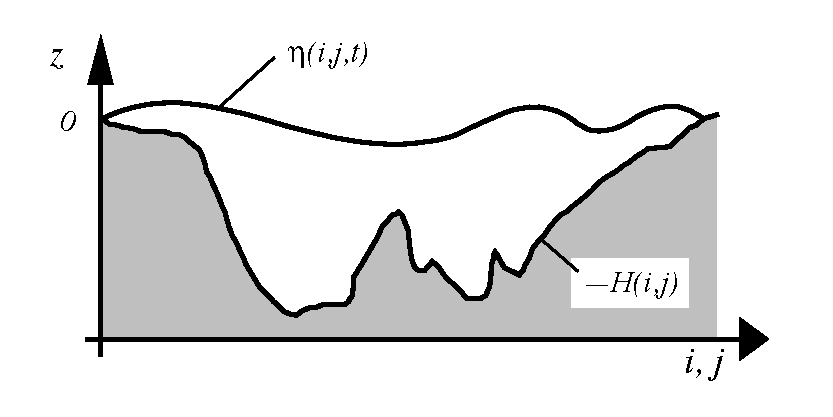
\includegraphics[width=0.90\textwidth]{./TexFiles/Figures/Fig_I_ocean_bc.pdf}
\caption{	 \label{Fig_ocean_bc} 
The ocean is bounded by two surfaces, $z=-H(i,j)$ and $z=\eta(i,j,t)$, where $H$ 
is the depth of the sea floor and $\eta$ the height of the sea surface. 
Both $H$ and $\eta$ are referenced to $z=0$.}
\end{center}   \end{figure}
%>>>>>>>>>>>>>>>>>>>>>>>>>>>>


\begin{description}
\item[Land - ocean interface:] the major flux between continental margins and the ocean is 
a mass exchange of fresh water through river runoff. Such an exchange modifies the sea 
surface salinity especially in the vicinity of major river mouths. It can be neglected for short 
range integrations but has to be taken into account for long term integrations as it influences 
the characteristics of water masses formed (especially at high latitudes). It is required in order 
to close the water cycle of the climate system. It is usually specified as a fresh water flux at 
the air-sea interface in the vicinity of river mouths.
\item[Solid earth - ocean interface:] heat and salt fluxes through the sea floor are small, 
except in special areas of little extent. They are usually neglected in the model 
\footnote{In fact, it has been shown that the heat flux associated with the solid Earth cooling 
($i.e.$the geothermal heating) is not negligible for the thermohaline circulation of the world 
ocean (see \ref{TRA_bbc}).}. 
The boundary condition is thus set to no flux of heat and salt across solid boundaries. 
For momentum, the situation is different. There is no flow across solid boundaries, 
$i.e.$ the velocity normal to the ocean bottom and coastlines is zero (in other words, 
the bottom velocity is parallel to solid boundaries). This kinematic boundary condition 
can be expressed as:
\begin{equation} \label{Eq_PE_w_bbc}
w = -{\rm {\bf U}}_h \cdot  \nabla _h \left( H \right)
\end{equation}
In addition, the ocean exchanges momentum with the earth through frictional processes. 
Such momentum transfer occurs at small scales in a boundary layer. It must be parameterized 
in terms of turbulent fluxes using bottom and/or lateral boundary conditions. Its specification 
depends on the nature of the physical parameterisation used for ${\rm {\bf D}}^{\rm {\bf U}}$ 
in \eqref{Eq_PE_dyn}. It is discussed in \S\ref{PE_zdf}, page~\pageref{PE_zdf}.% and Chap. III.6 to 9.
\item[Atmosphere - ocean interface:] the kinematic surface condition plus the mass flux 
of fresh water PE  (the precipitation minus evaporation budget) leads to: 
\begin{equation} \label{Eq_PE_w_sbc}
w = \frac{\partial \eta }{\partial t} 
    + \left. {{\rm {\bf U}}_h } \right|_{z=\eta } \cdot  \nabla _h \left( \eta \right) 
    + P-E
\end{equation}
The dynamic boundary condition, neglecting the surface tension (which removes capillary 
waves from the system) leads to the continuity of pressure across the interface $z=\eta$. 
The atmosphere and ocean also exchange horizontal momentum (wind stress), and heat.
\item[Sea ice - ocean interface:] the ocean and sea ice exchange heat, salt, fresh water 
and momentum. The sea surface temperature is constrained to be at the freezing point 
at the interface. Sea ice salinity is very low ($\sim4-6 \,psu$) compared to those of the 
ocean ($\sim34 \,psu$). The cycle of freezing/melting is associated with fresh water and 
salt fluxes that cannot be neglected.
\end{description}


%\newpage
%$\ $\newline    % force a new ligne

% ================================================================
% The Horizontal Pressure Gradient
% ================================================================
\section{The Horizontal Pressure Gradient }
\label{PE_hor_pg}

% -------------------------------------------------------------------------------------------------------------
% Pressure Formulation
% -------------------------------------------------------------------------------------------------------------
\subsection{Pressure Formulation}
\label{PE_p_formulation}

The total pressure at a given depth $z$ is composed of a surface pressure $p_s$ at a 
reference geopotential surface ($z=0$) and a hydrostatic pressure $p_h$ such that: 
$p(i,j,k,t)=p_s(i,j,t)+p_h(i,j,k,t)$. The latter is computed by integrating (\ref{Eq_PE_hydrostatic}), 
assuming that pressure in decibars can be approximated by depth in meters in (\ref{Eq_PE_eos}). 
The hydrostatic pressure is then given by:
\begin{equation} \label{Eq_PE_pressure}
p_h \left( {i,j,z,t} \right)
 = \int_{\varsigma =z}^{\varsigma =0} {g\;\rho \left( {T,S,\varsigma} \right)\;d\varsigma } 
\end{equation}
 Two strategies can be considered for the surface pressure term: $(a)$ introduce of a 
 new variable $\eta$, the free-surface elevation, for which a prognostic equation can be 
 established and solved; $(b)$ assume that the ocean surface is a rigid lid, on which the 
 pressure (or its horizontal gradient) can be diagnosed. When the former strategy is used, 
 one solution of the free-surface elevation consists of the excitation of external gravity waves. 
 The flow is barotropic and the surface moves up and down with gravity as the restoring force. 
 The phase speed of such waves is high (some hundreds of metres per second) so that 
 the time step would have to be very short if they were present in the model. The latter 
 strategy filters out these waves since the rigid lid approximation implies $\eta=0$, $i.e.$ 
 the sea surface is the surface $z=0$. This well known approximation increases the surface 
 wave speed to infinity and modifies certain other longwave dynamics ($e.g.$ barotropic 
 Rossby or planetary waves). The rigid-lid hypothesis is an obsolescent feature in modern 
 OGCMs. It has been available until the release 3.1 of  \NEMO, and it has been removed
 in release 3.2 and followings. Only the free surface formulation is now described in the
 this document (see the next sub-section).

% -------------------------------------------------------------------------------------------------------------
% Free Surface Formulation
% -------------------------------------------------------------------------------------------------------------
\subsection{Free Surface Formulation}
\label{PE_free_surface}

In the free surface formulation, a variable $\eta$, the sea-surface height, is introduced 
which describes the shape of the air-sea interface. This variable is solution of a 
prognostic equation which is established by forming the vertical average of the kinematic 
surface condition (\ref{Eq_PE_w_bbc}):
\begin{equation} \label{Eq_PE_ssh}
\frac{\partial \eta }{\partial t}=-D+P-E
 	\quad \text{where} \ 
D=\nabla \cdot \left[ {\left( {H+\eta } \right) \; {\rm{\bf \overline{U}}}_h \,} \right]
\end{equation}
and using (\ref{Eq_PE_hydrostatic}) the surface pressure is given by: $p_s = \rho \, g \, \eta$.

Allowing the air-sea interface to move introduces the external gravity waves (EGWs) 
as a class of solution of the primitive equations. These waves are barotropic because 
of hydrostatic assumption, and their phase speed is quite high. Their time scale is 
short with respect to the other processes described by the primitive equations.

Two choices can be made regarding the implementation of the free surface in the model, 
depending on the physical processes of interest. 

$\bullet$ If one is interested in EGWs, in particular the tides and their interaction 
with the baroclinic structure of the ocean (internal waves) possibly in shallow seas, 
then a non linear free surface is the most appropriate. This means that no 
approximation is made in (\ref{Eq_PE_ssh}) and that the variation of the ocean 
volume is fully taken into account. Note that in order to study the fast time scales 
associated with EGWs it is necessary to minimize time filtering effects (use an 
explicit time scheme with very small time step, or a split-explicit scheme with 
reasonably small time step, see \S\ref{DYN_spg_exp} or \S\ref{DYN_spg_ts}.

$\bullet$ If one is not interested in EGW but rather sees them as high frequency 
noise, it is possible to apply an explicit filter to slow down the fastest waves while 
not altering the slow barotropic Rossby waves. If further, an approximative conservation 
of heat and salt contents is sufficient for the problem solved, then it is 
sufficient to solve a linearized version of (\ref{Eq_PE_ssh}), which still allows 
to take into account freshwater fluxes applied at the ocean surface \citep{Roullet_Madec_JGR00}.

The filtering of EGWs in models with a free surface is usually a matter of discretisation 
of the temporal derivatives, using the time splitting method \citep{Killworth_al_JPO91, Zhang_Endoh_JGR92} 
or the implicit scheme \citep{Dukowicz1994}. In \NEMO, we use a slightly different approach 
developed by \citet{Roullet_Madec_JGR00}: the damping of EGWs is ensured by introducing an 
additional force in the momentum equation. \eqref{Eq_PE_dyn} becomes: 
\begin{equation} \label{Eq_PE_flt}
\frac{\partial {\rm {\bf U}}_h }{\partial t}= {\rm {\bf M}}
- g \nabla \left( \tilde{\rho} \ \eta \right) 
- g \ T_c \nabla \left( \widetilde{\rho} \ \partial_t \eta \right) 
\end{equation}
where $T_c$, is a parameter with dimensions of time which characterizes the force, 
$\widetilde{\rho} = \rho / \rho_o$ is the dimensionless density, and $\rm {\bf M}$ 
represents the collected contributions of the Coriolis, hydrostatic pressure gradient, 
non-linear and viscous terms in \eqref{Eq_PE_dyn}.

The new force can be interpreted as a diffusion of vertically integrated volume flux divergence. 
The time evolution of $D$ is thus governed by a balance of two terms, $-g$ \textbf{A} $\eta$ 
and $g \, T_c \,$ \textbf{A} $D$, associated with a propagative regime and a diffusive regime 
in the temporal spectrum, respectively. In the diffusive regime, the EGWs no longer propagate, 
$i.e.$ they are stationary and damped. The diffusion regime applies to the modes shorter than 
$T_c$. For longer ones, the diffusion term vanishes. Hence, the temporally unresolved EGWs 
can be damped by choosing $T_c > \rdt$. \citet{Roullet_Madec_JGR00} demonstrate that 
(\ref{Eq_PE_flt}) can be integrated with a leap frog scheme except the additional term which 
has to be computed implicitly. This is not surprising since the use of a large time step has a 
necessarily numerical cost. Two gains arise in comparison with the previous formulations. 
Firstly, the damping of EGWs can be quantified through the magnitude of the additional term. 
Secondly, the numerical scheme does not need any tuning. Numerical stability is ensured as 
soon as $T_c > \rdt$.

When the variations of free surface elevation are small compared to the thickness of the first 
model layer, the free surface equation (\ref{Eq_PE_ssh}) can be linearized. As emphasized 
by \citet{Roullet_Madec_JGR00} the linearization of (\ref{Eq_PE_ssh}) has consequences on the 
conservation of salt in the model. With the nonlinear free surface equation, the time evolution 
of the total salt content is 
\begin{equation} \label{Eq_PE_salt_content}
    \frac{\partial }{\partial t}\int\limits_{D\eta } {S\;dv} 
                        =\int\limits_S {S\;(-\frac{\partial \eta }{\partial t}-D+P-E)\;ds}
\end{equation}
where $S$ is the salinity, and the total salt is integrated over the whole ocean volume 
$D_\eta$ bounded by the time-dependent free surface. The right hand side (which is an 
integral over the free surface) vanishes when the nonlinear equation (\ref{Eq_PE_ssh}) 
is satisfied, so that the salt is perfectly conserved. When the free surface equation is 
linearized, \citet{Roullet_Madec_JGR00} show that the total salt content integrated in the fixed 
volume $D$ (bounded by the surface $z=0$) is no longer conserved:
\begin{equation} \label{Eq_PE_salt_content_linear}
         \frac{\partial }{\partial t}\int\limits_D {S\;dv} 
         		= - \int\limits_S {S\;\frac{\partial \eta }{\partial t}ds} 
\end{equation}

The right hand side of (\ref{Eq_PE_salt_content_linear}) is small in equilibrium solutions 
\citep{Roullet_Madec_JGR00}. It can be significant when the freshwater forcing is not balanced and 
the globally averaged free surface is drifting. An increase in sea surface height \textit{$\eta $} 
results in a decrease of the salinity in the fixed volume $D$. Even in that case though, 
the total salt integrated in the variable volume $D_{\eta}$ varies much less, since 
(\ref{Eq_PE_salt_content_linear}) can be rewritten as 
\begin{equation} \label{Eq_PE_salt_content_corrected}
\frac{\partial }{\partial t}\int\limits_{D\eta } {S\;dv} 
=\frac{\partial}{\partial t} \left[ \;{\int\limits_D {S\;dv} +\int\limits_S {S\eta \;ds} } \right]
=\int\limits_S {\eta \;\frac{\partial S}{\partial t}ds}
\end{equation}

Although the total salt content is not exactly conserved with the linearized free surface, 
its variations are driven by correlations of the time variation of surface salinity with the 
sea surface height, which is a negligible term. This situation contrasts with the case of 
the rigid lid approximation in which case freshwater forcing is represented by a virtual 
salt flux, leading to a spurious source of salt at the ocean surface 
\citep{Huang_JPO93, Roullet_Madec_JGR00}.

\newpage
$\ $\newline    % force a new ligne

% ================================================================
% Curvilinear z-coordinate System
% ================================================================
\section{Curvilinear \textit{z-}coordinate System}
\label{PE_zco}


% -------------------------------------------------------------------------------------------------------------
% Tensorial Formalism
% -------------------------------------------------------------------------------------------------------------
\subsection{Tensorial Formalism}
\label{PE_tensorial}

In many ocean circulation problems, the flow field has regions of enhanced dynamics 
($i.e.$ surface layers, western boundary currents, equatorial currents, or ocean fronts). 
The representation of such dynamical processes can be improved by specifically increasing 
the model resolution in these regions. As well, it may be convenient to use a lateral 
boundary-following coordinate system to better represent coastal dynamics. Moreover, 
the common geographical coordinate system has a singular point at the North Pole that 
cannot be easily treated in a global model without filtering. A solution consists of introducing 
an appropriate coordinate transformation that shifts the singular point onto land 
\citep{Madec_Imbard_CD96, Murray_JCP96}. As a consequence, it is important to solve the primitive 
equations in various curvilinear coordinate systems. An efficient way of introducing an 
appropriate coordinate transform can be found when using a tensorial formalism. 
This formalism is suited to any multidimensional curvilinear coordinate system. Ocean 
modellers mainly use three-dimensional orthogonal grids on the sphere (spherical earth 
approximation), with preservation of the local vertical. Here we give the simplified equations 
for this particular case. The general case is detailed by \citet{Eiseman1980} in their survey 
of the conservation laws of fluid dynamics.

Let (\textit{i},\textit{j},\textit{k}) be a set of orthogonal curvilinear coordinates on the sphere 
associated with the positively oriented orthogonal set of unit vectors (\textbf{i},\textbf{j},\textbf{k}) 
linked to the earth such that \textbf{k} is the local upward vector and (\textbf{i},\textbf{j}) are 
two vectors orthogonal to \textbf{k}, $i.e.$ along geopotential surfaces (Fig.\ref{Fig_referential}). 
Let $(\lambda,\varphi,z)$ be the geographical coordinate system in which a position is defined 
by the latitude $\varphi(i,j)$, the longitude $\lambda(i,j)$ and the distance from the centre of 
the earth $a+z(k)$ where $a$ is the earth's radius and $z$ the altitude above a reference sea 
level (Fig.\ref{Fig_referential}). The local deformation of the curvilinear coordinate system is 
given by $e_1$, $e_2$ and $e_3$, the three scale factors:
\begin{equation} \label{Eq_scale_factors}
\begin{aligned}
 e_1 &=\left( {a+z} \right)\;\left[ {\left( {\frac{\partial \lambda 
}{\partial i}\cos \varphi } \right)^2+\left( {\frac{\partial \varphi 
}{\partial i}} \right)^2} \right]^{1/2} \\ 
 e_2 &=\left( {a+z} \right)\;\left[ {\left( {\frac{\partial \lambda 
}{\partial j}\cos \varphi } \right)^2+\left( {\frac{\partial \varphi 
}{\partial j}} \right)^2} \right]^{1/2} \\ 
 e_3 &=\left( {\frac{\partial z}{\partial k}} \right) \\ 
 \end{aligned}
 \end{equation}

%>>>>>>>>>>>>>>>>>>>>>>>>>>>>
\begin{figure}[!tb] 	 \begin{center}
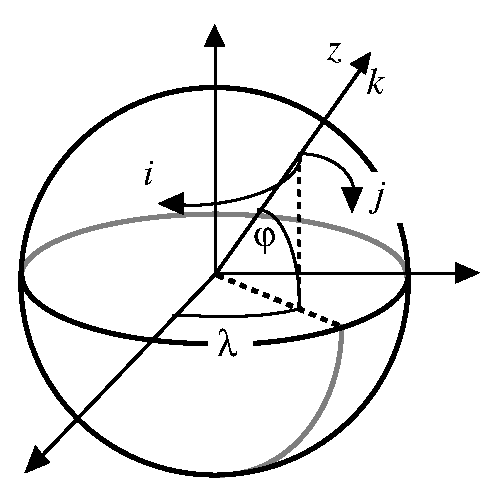
\includegraphics[width=0.60\textwidth]{./TexFiles/Figures/Fig_I_earth_referential.pdf}
\caption{	\label{Fig_referential} 
the geographical coordinate system $(\lambda,\varphi,z)$ and the curvilinear 
coordinate system (\textbf{i},\textbf{j},\textbf{k}). }
\end{center}   \end{figure}
%>>>>>>>>>>>>>>>>>>>>>>>>>>>>

Since the ocean depth is far smaller than the earth's radius, $a+z$, can be replaced by 
$a$ in (\ref{Eq_scale_factors}) (thin-shell approximation). The resulting horizontal scale 
factors $e_1$, $e_2$  are independent of $k$ while the vertical scale factor is a single 
function of $k$ as \textbf{k} is parallel to \textbf{z}. The scalar and vector operators that 
appear in the primitive equations (Eqs. \eqref{Eq_PE_dyn} to \eqref{Eq_PE_eos}) can 
be written in the tensorial form, invariant in any orthogonal horizontal curvilinear coordinate 
system transformation:
\begin{subequations} \label{Eq_PE_discrete_operators}
\begin{equation} \label{Eq_PE_grad}
\nabla q=\frac{1}{e_1 }\frac{\partial q}{\partial i}\;{\rm {\bf 
i}}+\frac{1}{e_2 }\frac{\partial q}{\partial j}\;{\rm {\bf j}}+\frac{1}{e_3 
}\frac{\partial q}{\partial k}\;{\rm {\bf k}}    \\
\end{equation}
\begin{equation} \label{Eq_PE_div}
\nabla \cdot {\rm {\bf A}} 
= \frac{1}{e_1 \; e_2} \left[ 
  \frac{\partial \left(e_2 \; a_1\right)}{\partial i }
+\frac{\partial \left(e_1 \; a_2\right)}{\partial j }    	\right]
+ \frac{1}{e_3} \left[ \frac{\partial a_3}{\partial k }   \right]
\end{equation}
\begin{equation} \label{Eq_PE_curl}
   \begin{split}
\nabla \times \vect{A} = 
    \left[ {\frac{1}{e_2 }\frac{\partial a_3}{\partial j}
            -\frac{1}{e_3 }\frac{\partial a_2 }{\partial k}} \right] \; \vect{i}
&+\left[ {\frac{1}{e_3 }\frac{\partial a_1 }{\partial k}
           -\frac{1}{e_1 }\frac{\partial a_3 }{\partial i}} \right] \; \vect{j} 		\\
&+\frac{1}{e_1 e_2 } \left[ {\frac{\partial \left( {e_2 a_2 } \right)}{\partial i}
                                       -\frac{\partial \left( {e_1 a_1 } \right)}{\partial j}} \right] \; \vect{k} 
   \end{split}
\end{equation}
\begin{equation} \label{Eq_PE_lap}
\Delta q = \nabla \cdot \left(  \nabla q \right)
\end{equation}
\begin{equation} \label{Eq_PE_lap_vector}
\Delta {\rm {\bf A}} =
  \nabla \left( \nabla \cdot {\rm {\bf A}} \right)
- \nabla \times \left(  \nabla \times {\rm {\bf A}} \right)
\end{equation}
\end{subequations}
where $q$ is a scalar quantity and ${\rm {\bf A}}=(a_1,a_2,a_3)$ a vector in the $(i,j,k)$ coordinate system.

% -------------------------------------------------------------------------------------------------------------
% Continuous Model Equations
% -------------------------------------------------------------------------------------------------------------
\subsection{Continuous Model Equations}
\label{PE_zco_Eq}

In order to express the Primitive Equations in tensorial formalism, it is necessary to compute 
the horizontal component of the non-linear and viscous terms of the equation using 
\eqref{Eq_PE_grad}) to \eqref{Eq_PE_lap_vector}. 
Let us set $\vect U=(u,v,w)={\vect{U}}_h +w\;\vect{k}$, the velocity in the $(i,j,k)$ coordinate 
system and define the relative vorticity $\zeta$ and the divergence of the horizontal velocity 
field $\chi$, by:
\begin{equation} \label{Eq_PE_curl_Uh}
\zeta =\frac{1}{e_1 e_2 }\left[ {\frac{\partial \left( {e_2 \,v} 
\right)}{\partial i}-\frac{\partial \left( {e_1 \,u} \right)}{\partial j}} 
\right]
\end{equation}
\begin{equation} \label{Eq_PE_div_Uh}
\chi =\frac{1}{e_1 e_2 }\left[ {\frac{\partial \left( {e_2 \,u} 
\right)}{\partial i}+\frac{\partial \left( {e_1 \,v} \right)}{\partial j}} 
\right]
\end{equation}

Using the fact that the horizontal scale factors $e_1$ and $e_2$ are independent of $k$ 
and that $e_3$  is a function of the single variable $k$, the nonlinear term of 
\eqref{Eq_PE_dyn} can be transformed as follows:
\begin{flalign*}
&\left[ {\left( {	\nabla \times {\rm {\bf U}}    } \right) \times {\rm {\bf U}}
+\frac{1}{2}	\nabla \left( {{\rm {\bf U}}^2} \right)}	 \right]_h 			&
\end{flalign*}
\begin{flalign*}
&\qquad=\left( {{\begin{array}{*{20}c}
 {\left[ 	{	 \frac{1}{e_3}	\frac{\partial u	}{\partial k}
			-\frac{1}{e_1}	\frac{\partial w	}{\partial i} } \right] w - \zeta \; v } 	 	\\
 		{\zeta \; u - \left[ {	 \frac{1}{e_2} \frac{\partial w}{\partial j}
							-\frac{1}{e_3} \frac{\partial v}{\partial k} } \right] \ w}	 \\
		 \end{array} }} \right)			
+\frac{1}{2}	\left( {{\begin{array}{*{20}c}
		 {	\frac{1}{e_1}	\frac{\partial \left( u^2+v^2+w^2 \right)}{\partial i}} 	\hfill	 \\
		 {	\frac{1}{e_2}	\frac{\partial \left( u^2+v^2+w^2 \right)}{\partial j}} 	\hfill	 \\
		 \end{array} }} \right)			&
\end{flalign*}
\begin{flalign*}
& \qquad =\left( {{	\begin{array}{*{20}c}
 {-\zeta \; v} \hfill \\
 { \zeta \; u} \hfill \\
			\end{array} }} \right)
+\frac{1}{2}\left( {{	\begin{array}{*{20}c}
 {\frac{1}{e_1 }\frac{\partial \left( {u^2+v^2} \right)}{\partial i}} \hfill 	\\
 {\frac{1}{e_2 }\frac{\partial \left( {u^2+v^2} \right)}{\partial j}} \hfill 	\\
						\end{array} }} \right)			
+\frac{1}{e_3 }\left( {{		\begin{array}{*{20}c}
 { w \; \frac{\partial u}{\partial k}} 	\\
 { w \; \frac{\partial v}{\partial k}} 	\\
							\end{array} }} \right)	
-\left( {{	\begin{array}{*{20}c}
 {\frac{w}{e_1}\frac{\partial w}{\partial i}
 -\frac{1}{2e_1}\frac{\partial w^2}{\partial i}} \hfill \\
 {\frac{w}{e_2}\frac{\partial w}{\partial j}
  -\frac{1}{2e_2}\frac{\partial w^2}{\partial j}} \hfill \\
			\end{array} }} \right) 			&
\end{flalign*}

The last term of the right hand side is obviously zero, and thus the nonlinear term of 
\eqref{Eq_PE_dyn} is written in the $(i,j,k)$ coordinate system:
\begin{equation} \label{Eq_PE_vector_form}
\left[ {\left( {	\nabla \times {\rm {\bf U}}    } \right) \times {\rm {\bf U}}
+\frac{1}{2}	\nabla \left( {{\rm {\bf U}}^2} \right)}	 \right]_h 
=\zeta 
\;{\rm {\bf k}}\times {\rm {\bf U}}_h +\frac{1}{2}\nabla _h \left( {{\rm 
{\bf U}}_h^2 } \right)+\frac{1}{e_3 }w\frac{\partial {\rm {\bf U}}_h 
}{\partial k}   	
\end{equation}

This is the so-called \textit{vector invariant form} of the momentum advection term. 
For some purposes, it can be advantageous to write this term in the so-called flux form, 
$i.e.$ to write it as the divergence of fluxes. For example, the first component of 
\eqref{Eq_PE_vector_form} (the $i$-component) is transformed as follows:
\begin{flalign*}
&{	\begin{array}{*{20}l}
\left[ {\left( {\nabla \times \vect{U}} \right)\times \vect{U}
          +\frac{1}{2}\nabla \left( {\vect{U}}^2 \right)} \right]_i   % \\
%\\
     = - \zeta \;v 
     + \frac{1}{2\;e_1 } \frac{\partial \left( {u^2+v^2} \right)}{\partial i}
     + \frac{1}{e_3}w \ \frac{\partial u}{\partial k} 			\\
\\
\qquad =\frac{1}{e_1 \; e_2} \left( 	-v\frac{\partial \left( {e_2 \,v} \right)}{\partial i}
							+v\frac{\partial \left( {e_1 \,u} \right)}{\partial j}	 \right)
+\frac{1}{e_1 e_2 }\left( 	+e_2 \; u\frac{\partial u}{\partial i}
 							+e_2 \; v\frac{\partial v}{\partial i}	  				 \right) 
+\frac{1}{e_3}       \left( 	w\;\frac{\partial u}{\partial k} 		\right)   \\
\end{array} } 			&
\end{flalign*}
\begin{flalign*}
&{	\begin{array}{*{20}l}
\qquad =\frac{1}{e_1 \; e_2} 	\left\{ 
 -\left(   	    v^2 	\frac{\partial e_2                                }{\partial i} 
 		+e_2 \,v		\frac{\partial v                                   }{\partial i}  	\right)
+\left( 				\frac{\partial \left( {e_1 \,u\,v} 	\right)}{\partial j}
		-e_1 \,u		\frac{\partial v                                   }{\partial j} 	\right) 	\right. 
\\  \left.	\qquad \qquad \quad
+\left( 				\frac{\partial \left( {e_2 u\,u}     \right)}{\partial i}
		-u			\frac{\partial \left( {e_2 u}         \right)}{\partial i} 	\right)
+e_2 v		 		\frac{\partial v                                    }{\partial i}
 						\right\} 
+\frac{1}{e_3} \left(
 					\frac{\partial \left( {w\,u} \right)         }{\partial k}
		 -u			\frac{\partial w 						   }{\partial k} 	\right) \\
\end{array} } 		&
\end{flalign*}
\begin{flalign*}
&{	\begin{array}{*{20}l}
\qquad =\frac{1}{e_1 \; e_2} 	\left( 
					\frac{\partial \left( {e_2 \,u\,u} \right)}{\partial i}
		+			\frac{\partial \left( {e_1 \,u\,v} \right)}{\partial j}	\right)
+\frac{1}{e_3 }		\frac{\partial \left( {w\,u		 } \right)}{\partial k}
\\  \qquad \qquad \quad
+\frac{1}{e_1 e_2 }		\left( 
 		-u	\left( 	\frac{\partial \left( {e_1 v	 } \right)}{\partial j}
	 				-v\,\frac{\partial e_1 }{\partial j}				 \right)
		-u			\frac{\partial \left( {e_2 u	 } \right)}{\partial i}
						\right)
 -\frac{1}{e_3 }	 	\frac{\partial w}{\partial k}	u
 +\frac{1}{e_1 e_2 }\left( 	-v^2\frac{\partial e_2	 }{\partial i}		 \right)	
\end{array} } 		&
\end{flalign*}
\begin{flalign*}
&{	\begin{array}{*{20}l}
\qquad = \nabla \cdot \left( {{\rm {\bf U}}\,u}	\right)
-   \left( \nabla \cdot {\rm {\bf U}} \right) \ u
+\frac{1}{e_1 e_2 }\left( 
		-v^2		\frac{\partial e_2 }{\partial i}
		+uv	\,		\frac{\partial e_1 }{\partial j} 	\right) \\
\end{array} } 		&
\end{flalign*}
as $\nabla \cdot {\rm {\bf U}}\;=0$ (incompressibility) it comes:
\begin{flalign*}
&{	\begin{array}{*{20}l}
\qquad = \nabla \cdot \left( 	{{\rm {\bf U}}\,u}		\right)
+	\frac{1}{e_1 e_2 }   \left( v \; \frac{\partial e_2}{\partial i}
						       -u \; \frac{\partial e_1}{\partial j} 	\right)  \left( -v \right)	
\end{array} } 		&
\end{flalign*}

The flux form of the momentum advection term is therefore given by:
\begin{multline} \label{Eq_PE_flux_form}
		\left[ 
  \left( 	{\nabla \times {\rm {\bf U}}} 	\right) \times {\rm {\bf U}}
+\frac{1}{2}	\nabla \left( 	{{\rm {\bf U}}^2} 	\right)
		\right]_h 
\\
= \nabla \cdot 	\left( {{\begin{array}{*{20}c}	{\rm {\bf U}} \, u 	\hfill \\
												{\rm {\bf U}} \, v	\hfill \\
						\end{array} }} 	
				\right)
+\frac{1}{e_1 e_2 }		\left( 
		 v\frac{\partial e_2}{\partial i}
		-u\frac{\partial e_1}{\partial j} 
						\right) {\rm {\bf k}} \times {\rm {\bf U}}_h
\end{multline}

The flux form has two terms, the first one is expressed as the divergence of momentum 
fluxes (hence the flux form name given to this formulation) and the second one is due to 
the curvilinear nature of the coordinate system used. The latter is called the \emph{metric} 
term and can be viewed as a modification of the Coriolis parameter: 
\begin{equation} \label{Eq_PE_cor+metric}
f \to f + \frac{1}{e_1\;e_2}  \left(  v \frac{\partial e_2}{\partial i}
					         -u \frac{\partial e_1}{\partial j}  \right)
\end{equation}

Note that in the case of geographical coordinate, $i.e.$ when $(i,j) \to (\lambda ,\varphi )$ 
and $(e_1 ,e_2) \to (a \,\cos \varphi ,a)$, we recover the commonly used modification of 
the Coriolis parameter $f \to f+(u/a) \tan \varphi$.


$\ $\newline    % force a new ligne

To sum up, the curvilinear $z$-coordinate equations solved by the ocean model can be 
written in the following tensorial formalism:

\vspace{+10pt}
$\bullet$ \textbf{Vector invariant form of the momentum equations} :

\begin{subequations} \label{Eq_PE_dyn_vect}
\begin{equation} \label{Eq_PE_dyn_vect_u} \begin{split}
\frac{\partial u}{\partial t} 
= +   \left( {\zeta +f} \right)\,v                                    
   -   \frac{1}{2\,e_1}           \frac{\partial}{\partial i} \left(  u^2+v^2   \right) 
   -   \frac{1}{e_3    }  w     \frac{\partial u}{\partial k}      &      \\
   -   \frac{1}{e_1    }            \frac{\partial}{\partial i} \left( \frac{p_s+p_h }{\rho _o}    \right)    
   &+   D_u^{\vect{U}}  +   F_u^{\vect{U}}      \\
\\
\frac{\partial v}{\partial t} =
       -   \left( {\zeta +f} \right)\,u   
       -   \frac{1}{2\,e_2 }        \frac{\partial }{\partial j}\left(  u^2+v^2  \right)   
       -   \frac{1}{e_3     }   w  \frac{\partial v}{\partial k}     &      \\
       -   \frac{1}{e_2     }        \frac{\partial }{\partial j}\left( \frac{p_s+p_h }{\rho _o}  \right)    
    &+  D_v^{\vect{U}}  +   F_v^{\vect{U}}
\end{split} \end{equation}
\end{subequations}


\vspace{+10pt}
$\bullet$ \textbf{flux form of the momentum equations} :
\begin{subequations} \label{Eq_PE_dyn_flux}
\begin{multline} \label{Eq_PE_dyn_flux_u}
\frac{\partial u}{\partial t}=
+   \left( { f + \frac{1}{e_1 \; e_2}
					\left( 	 v \frac{\partial e_2}{\partial i}
						-u \frac{\partial e_1}{\partial j} 	\right)} 	\right) \, v    \\
- \frac{1}{e_1 \; e_2} 	\left( 
					\frac{\partial \left( {e_2 \,u\,u} \right)}{\partial i}
		+			\frac{\partial \left( {e_1 \,v\,u} \right)}{\partial j}	\right)
                 - \frac{1}{e_3 }\frac{\partial \left( {         w\,u} \right)}{\partial k}    \\
-   \frac{1}{e_1 }\frac{\partial}{\partial i}\left( \frac{p_s+p_h }{\rho _o}   \right)
+   D_u^{\vect{U}} +   F_u^{\vect{U}}
\end{multline}
\begin{multline} \label{Eq_PE_dyn_flux_v}
\frac{\partial v}{\partial t}=
-   \left( { f + \frac{1}{e_1 \; e_2}
					\left( 	 v \frac{\partial e_2}{\partial i}
						-u \frac{\partial e_1}{\partial j} 	\right)} 	\right) \, u   \\
 \frac{1}{e_1 \; e_2} 	\left( 
					\frac{\partial \left( {e_2 \,u\,v} \right)}{\partial i}
		+			\frac{\partial \left( {e_1 \,v\,v} \right)}{\partial j}	\right)
                 - \frac{1}{e_3 } \frac{\partial \left( {        w\,v} \right)}{\partial k}    \\
-   \frac{1}{e_2 }\frac{\partial }{\partial j}\left( \frac{p_s+p_h }{\rho _o}    \right)
+  D_v^{\vect{U}} +  F_v^{\vect{U}} 
\end{multline}
\end{subequations}
where $\zeta$, the relative vorticity, is given by \eqref{Eq_PE_curl_Uh} and $p_s $, 
the surface pressure, is given by:
\begin{equation} \label{Eq_PE_spg}
p_s = \left\{ \begin{split} 
\rho \,g \,\eta &                                 \qquad  \qquad  \;   \qquad \text{ standard free surface} \\ 
\rho \,g \,\eta &+ \rho_o \,\mu \,\frac{\partial \eta }{\partial t}      \qquad \text{ filtered     free surface}    
\end{split} 
\right.
\end{equation}
with $\eta$ is solution of \eqref{Eq_PE_ssh}

The vertical velocity and the hydrostatic pressure are diagnosed from the following equations:
\begin{equation} \label{Eq_w_diag}
\frac{\partial w}{\partial k}=-\chi \;e_3 
\end{equation}
\begin{equation} \label{Eq_hp_diag}
\frac{\partial p_h }{\partial k}=-\rho \;g\;e_3 
\end{equation}
where the divergence of the horizontal velocity, $\chi$ is given by \eqref{Eq_PE_div_Uh}.

\vspace{+10pt}
$\bullet$ \textit{tracer equations} :
\begin{equation} \label{Eq_S}
\frac{\partial T}{\partial t} = 
-\frac{1}{e_1 e_2 }\left[ {	   \frac{\partial \left( {e_2 T\,u} \right)}{\partial i}
						+\frac{\partial \left( {e_1 T\,v} \right)}{\partial j}} \right]
-\frac{1}{e_3 }\frac{\partial \left( {T\,w} \right)}{\partial k} + D^T + F^T
\end{equation}
\begin{equation} \label{Eq_T}
\frac{\partial S}{\partial t} = 
-\frac{1}{e_1 e_2 }\left[ 	  {\frac{\partial \left( {e_2 S\,u} \right)}{\partial i}
						+\frac{\partial \left( {e_1 S\,v} \right)}{\partial j}} \right]
-\frac{1}{e_3 }\frac{\partial \left( {S\,w} \right)}{\partial k} + D^S + F^S
\end{equation}
\begin{equation} \label{Eq_rho}
\rho =\rho \left( {T,S,z(k)} \right)
\end{equation}

The expression of \textbf{D}$^{U}$, $D^{S}$ and $D^{T}$ depends on the subgrid scale 
parameterisation used. It will be defined in \S\ref{PE_zdf}. The nature and formulation of 
${\rm {\bf F}}^{\rm {\bf U}}$, $F^T$ and $F^S$, the surface forcing terms, are discussed 
in Chapter~\ref{SBC}.


\newpage 
$\ $\newline    % force a new ligne
% ================================================================
% Curvilinear generalised vertical coordinate System
% ================================================================
\section{Curvilinear generalised vertical coordinate System}
\label{PE_gco}

The ocean domain presents a huge diversity of situation in the vertical. First the ocean surface is a time dependent surface (moving surface). Second the ocean floor depends on the geographical position, varying from more than 6,000 meters in abyssal trenches to zero at the coast. Last but not least, the ocean stratification exerts a strong barrier to vertical motions and mixing. 
Therefore, in order to represent the ocean with respect to the first point a space and time dependent vertical coordinate that follows the variation of the sea surface height $e.g.$ an $z$*-coordinate; for the second point, a space variation to fit the change of bottom topography $e.g.$ a terrain-following or $\sigma$-coordinate; and for the third point, one will be tempted to use a space and time dependent coordinate that follows the isopycnal surfaces, $e.g.$ an isopycnic coordinate.

In order to satisfy two or more constrains one can even be tempted to mixed these coordinate systems, as in HYCOM (mixture of $z$-coordinate at the surface, isopycnic coordinate in the ocean interior and $\sigma$ at the ocean bottom) \citep{Chassignet_al_JPO03}  or OPA (mixture of $z$-coordinate in vicinity the surface and steep topography areas and $\sigma$-coordinate elsewhere) \citep{Madec_al_JPO96} among others.

In fact one is totally free to choose any space and time vertical coordinate by introducing an arbitrary vertical coordinate :
\begin{equation} \label{Eq_s}
s=s(i,j,k,t)
\end{equation}
with the restriction that the above equation gives a single-valued monotonic relationship between $s$ and $k$, when $i$, $j$ and $t$ are held fixed. \eqref{Eq_s} is a transformation from the $(i,j,k,t)$ coordinate system with independent variables into the $(i,j,s,t)$ generalised coordinate system with $s$ depending on the other three variables through \eqref{Eq_s}.
This so-called \textit{generalised vertical coordinate} \citep{Kasahara_MWR74} is in fact an Arbitrary Lagrangian--Eulerian (ALE) coordinate. Indeed, choosing an expression for $s$ is an arbitrary choice that determines which part of the vertical velocity (defined from a fixed referential) will cross the levels (Eulerian part) and which part will be used to move them (Lagrangian part).
The coordinate is also sometime referenced as an adaptive coordinate \citep{Hofmeister_al_OM09}, since the coordinate system is adapted in the course of the simulation. Its most often used implementation is via an ALE algorithm, in which a pure lagrangian step is followed by regridding and remapping steps, the later step implicitly embedding the vertical advection \citep{Hirt_al_JCP74, Chassignet_al_JPO03, White_al_JCP09}. Here we follow the \citep{Kasahara_MWR74} strategy : a regridding step (an update of the vertical coordinate) followed by an eulerian step with an explicit computation of vertical advection relative to the moving s-surfaces.

%\gmcomment{

%A key point here is that the $s$-coordinate depends on $(i,j)$ ==> horizontal pressure gradient...

the generalized vertical coordinates used in ocean modelling are not orthogonal, 
which contrasts with many other applications in mathematical physics. 
Hence, it is useful to keep in mind the following properties that may seem 
odd on initial encounter.

The horizontal velocity in ocean models measures motions in the horizontal plane, 
perpendicular to the local gravitational field. That is, horizontal velocity is mathematically 
the same regardless the vertical coordinate, be it geopotential, isopycnal, pressure, 
or terrain following. The key motivation for maintaining the same horizontal velocity 
component is that the hydrostatic and geostrophic balances are dominant in the large-scale ocean. 
Use of an alternative quasi-horizontal velocity, for example one oriented parallel 
to the generalized surface, would lead to unacceptable numerical errors. 
Correspondingly, the vertical direction is anti-parallel to the gravitational force in all 
of the coordinate systems. We do not choose the alternative of a quasi-vertical 
direction oriented normal to the surface of a constant generalized vertical coordinate. 

It is the method used to measure transport across the generalized vertical coordinate 
surfaces which differs between the vertical coordinate choices. That is, computation 
of the dia-surface velocity component represents the fundamental distinction between 
the various coordinates. In some models, such as geopotential, pressure, and 
terrain following, this transport is typically diagnosed from volume or mass conservation. 
In other models, such as isopycnal layered models, this transport is prescribed based 
on assumptions about the physical processes producing a flux across the layer interfaces. 


In this section we first establish the PE in the generalised vertical $s$-coordinate, 
then we discuss the particular cases available in \NEMO, namely $z$, $z$*, $s$, and $\tilde z$.  
%}

% -------------------------------------------------------------------------------------------------------------
% The s-coordinate Formulation
% -------------------------------------------------------------------------------------------------------------
\subsection{The \textit{s-}coordinate Formulation}

Starting from the set of equations established in \S\ref{PE_zco} for the special case $k=z$ 
and thus $e_3=1$, we introduce an arbitrary vertical coordinate $s=s(i,j,k,t)$, which includes 
$z$-, \textit{z*}- and $\sigma-$coordinates as special cases ($s=z$, $s=\textit{z*}$, and 
$s=\sigma=z/H$ or $=z/\left(H+\eta \right)$, resp.). A formal derivation of the transformed 
equations is given in Appendix~\ref{Apdx_A}. Let us define the vertical scale factor by 
$e_3=\partial_s z$  ($e_3$ is now a function of $(i,j,k,t)$ ), and the slopes in the 
(\textbf{i},\textbf{j}) directions between $s-$ and $z-$surfaces by :
\begin{equation} \label{Eq_PE_sco_slope}
\sigma _1 =\frac{1}{e_1 }\;\left. {\frac{\partial z}{\partial i}} \right|_s 
\quad \text{, and } \quad 
\sigma _2 =\frac{1}{e_2 }\;\left. {\frac{\partial z}{\partial j}} \right|_s
\end{equation}
We also introduce  $\omega $, a dia-surface velocity component, defined as the velocity 
relative to the moving $s$-surfaces and normal to them:
\begin{equation} \label{Eq_PE_sco_w}
\omega  = w - e_3 \, \frac{\partial s}{\partial t} - \sigma _1 \,u - \sigma _2 \,v    \\
\end{equation}

The equations solved by the ocean model \eqref{Eq_PE} in $s-$coordinate can be written as follows:

 \vspace{0.5cm}
* momentum equation:
\begin{multline} \label{Eq_PE_sco_u}
\frac{1}{e_3} \frac{\partial \left(  e_3\,u  \right) }{\partial t}=
	+   \left( {\zeta +f} \right)\,v                                    
	-   \frac{1}{2\,e_1} \frac{\partial}{\partial i} \left(  u^2+v^2   \right) 
	-   \frac{1}{e_3} \omega \frac{\partial u}{\partial k}       \\
	-   \frac{1}{e_1} \frac{\partial}{\partial i} \left( \frac{p_s + p_h}{\rho _o}    \right)    
	+  g\frac{\rho }{\rho _o}\sigma _1 
	+   D_u^{\vect{U}}  +   F_u^{\vect{U}} \quad
\end{multline}
\begin{multline} \label{Eq_PE_sco_v}
\frac{1}{e_3} \frac{\partial \left(  e_3\,v  \right) }{\partial t}=
	-   \left( {\zeta +f} \right)\,u   
	-   \frac{1}{2\,e_2 }\frac{\partial }{\partial j}\left(  u^2+v^2  \right)     	
	-   \frac{1}{e_3 } \omega \frac{\partial v}{\partial k}         \\
	-   \frac{1}{e_2 }\frac{\partial }{\partial j}\left( \frac{p_s+p_h }{\rho _o}  \right) 
	 +  g\frac{\rho }{\rho _o }\sigma _2   
	+  D_v^{\vect{U}}  +   F_v^{\vect{U}} \quad
\end{multline}
where the relative vorticity, \textit{$\zeta $}, the surface pressure gradient, and the hydrostatic 
pressure have the same expressions as in $z$-coordinates although they do not represent 
exactly the same quantities. $\omega$ is provided by the continuity equation 
(see Appendix~\ref{Apdx_A}):

\begin{equation} \label{Eq_PE_sco_continuity}
\frac{\partial e_3}{\partial t} + e_3 \; \chi + \frac{\partial \omega }{\partial s} = 0   
\qquad \text{with }\;\;  
\chi =\frac{1}{e_1 e_2 e_3 }\left[ {\frac{\partial \left( {e_2 e_3 \,u} 
\right)}{\partial i}+\frac{\partial \left( {e_1 e_3 \,v} \right)}{\partial 
j}} \right]
\end{equation}

 \vspace{0.5cm}
* tracer equations:
\begin{multline} \label{Eq_PE_sco_t}
\frac{1}{e_3} \frac{\partial \left(  e_3\,T  \right) }{\partial t}=
-\frac{1}{e_1 e_2 e_3 }\left[ {\frac{\partial \left( {e_2 e_3\,u\,T} \right)}{\partial i}
                                           +\frac{\partial \left( {e_1 e_3\,v\,T} \right)}{\partial j}} \right]   \\
-\frac{1}{e_3 }\frac{\partial \left( {T\,\omega } \right)}{\partial k}   + D^T + F^S   \qquad
\end{multline}

\begin{multline} \label{Eq_PE_sco_s}
\frac{1}{e_3} \frac{\partial \left(  e_3\,S  \right) }{\partial t}=
-\frac{1}{e_1 e_2 e_3 }\left[ {\frac{\partial \left( {e_2 e_3\,u\,S} \right)}{\partial i}
                                           +\frac{\partial \left( {e_1 e_3\,v\,S} \right)}{\partial j}} \right]    \\
-\frac{1}{e_3 }\frac{\partial \left( {S\,\omega } \right)}{\partial k}     + D^S + F^S   \qquad
\end{multline}

The equation of state has the same expression as in $z$-coordinate, and similar expressions 
are used for mixing and forcing terms.

\gmcomment{
\colorbox{yellow}{ to be updated $= = >$}
Add a few works on z and zps and s and underlies the differences between all of them
\colorbox{yellow}{ $< = =$ end update}  }



% -------------------------------------------------------------------------------------------------------------
% Curvilinear z*-coordinate System
% -------------------------------------------------------------------------------------------------------------
\subsection{Curvilinear \textit{z*}--coordinate System}
\label{PE_zco_star}

%>>>>>>>>>>>>>>>>>>>>>>>>>>>>
\begin{figure}[!b] 	 \begin{center}
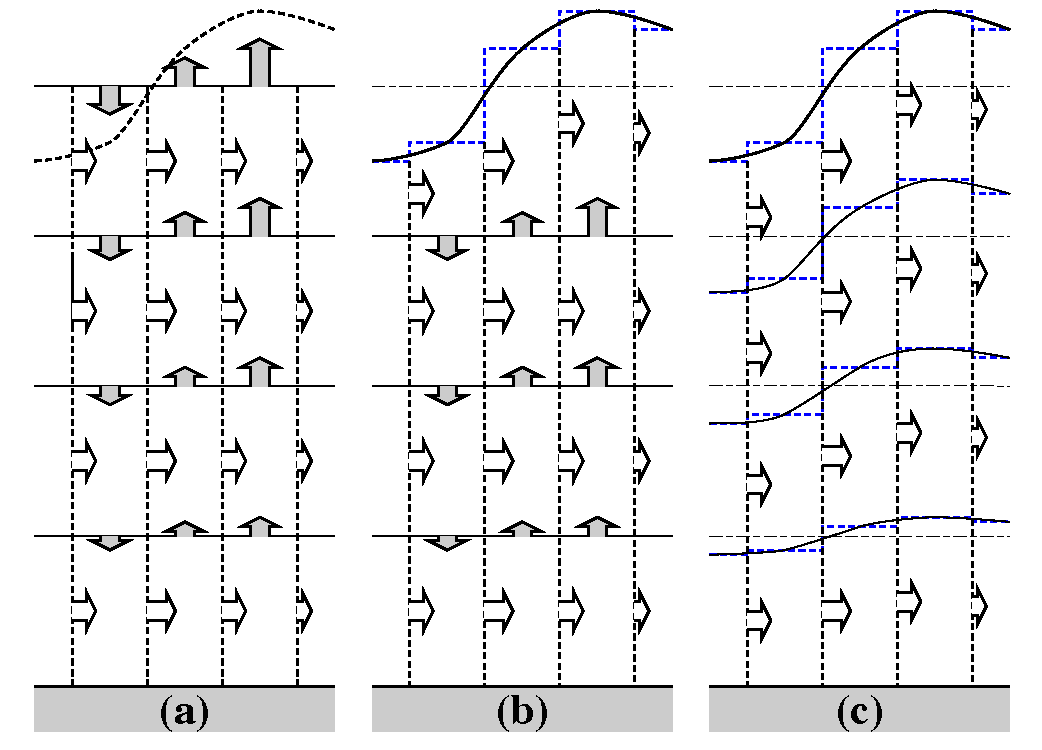
\includegraphics[width=1.0\textwidth]{./TexFiles/Figures/Fig_z_zstar.pdf}
\caption{	\label{Fig_z_zstar} 
(a) $z$-coordinate in linear free-surface case ; 
(b) $z-$coordinate in non-linear free surface case ; 
(c) re-scaled height coordinate (become popular as the \textit{z*-}coordinate 
\citep{Adcroft_Campin_OM04} ).}
\end{center}   \end{figure}
%>>>>>>>>>>>>>>>>>>>>>>>>>>>>


In that case, the free surface equation is nonlinear, and the variations of volume are fully 
taken into account. These coordinates systems is presented in a report \citep{Levier2007} 
available on the \NEMO web site. 

%\gmcomment{
The \textit{z*} coordinate approach is an unapproximated, non-linear free surface implementation 
which allows one to deal with large amplitude free-surface
variations relative to the vertical resolution \citep{Adcroft_Campin_OM04}. In
the  \textit{z*} formulation, the variation of the column thickness due to sea-surface
undulations is not concentrated in the surface level, as in the $z$-coordinate formulation,
but is equally distributed over the full water column. Thus vertical
levels naturally follow sea-surface variations, with a linear attenuation with
depth, as illustrated by figure fig.1c . Note that with a flat bottom, such as in
fig.1c, the bottom-following  $z$ coordinate and  \textit{z*} are equivalent.
The definition and modified oceanic equations for the rescaled vertical coordinate
 \textit{z*}, including the treatment of fresh-water flux at the surface, are
detailed in Adcroft and Campin (2004). The major points are summarized
here. The position ( \textit{z*}) and vertical discretization (\textit{z*}) are expressed as:
\begin{equation} \label{Eq_z-star}
H +  \textit{z*} = (H + z) / r \quad \text{and} \ \delta \textit{z*} = \delta z / r \quad \text{with} \ r = \frac{H+\eta} {H}
\end{equation} 
Since the vertical displacement of the free surface is incorporated in the vertical
coordinate  \textit{z*}, the upper and lower boundaries are at fixed  \textit{z*} position,  
$\textit{z*} = 0$ and  $\textit{z*} = -H$ respectively. Also the divergence of the flow field 
is no longer zero as shown by the continuity equation:
\begin{equation*} 
\frac{\partial r}{\partial t} = \nabla_{\textit{z*}} \cdot \left( r \; \rm{\bf U}_h \right)
		\left( r \; w\textit{*} \right) = 0 
\end{equation*} 
%}


% from MOM4p1 documentation

To overcome problems with vanishing surface and/or bottom cells, we consider the 
zstar coordinate 
\begin{equation} \label{PE_}
	z^\star = H \left( \frac{z-\eta}{H+\eta} \right)
\end{equation}

This coordinate is closely related to the "eta" coordinate used in many atmospheric 
models (see Black (1994) for a review of eta coordinate atmospheric models). It 
was originally used in ocean models by Stacey et al. (1995) for studies of tides 
next to shelves, and it has been recently promoted by Adcroft and Campin (2004) 
for global climate modelling.

The surfaces of constant $z^\star$ are quasi-horizontal. Indeed, the $z^\star$ coordinate reduces to $z$ when $\eta$ is zero. In general, when noting the large differences between 
undulations of the bottom topography versus undulations in the surface height, it 
is clear that surfaces constant $z^\star$ are very similar to the depth surfaces. These properties greatly reduce difficulties of computing the horizontal pressure gradient relative to terrain following sigma models discussed in \S\ref{PE_sco}. 
Additionally, since $z^\star$ when $\eta = 0$, no flow is spontaneously generated in an 
unforced ocean starting from rest, regardless the bottom topography. This behaviour is in contrast to the case with "s"-models, where pressure gradient errors in 
the presence of nontrivial topographic variations can generate nontrivial spontaneous flow from a resting state, depending on the sophistication of the pressure 
gradient solver. The quasi-horizontal nature of the coordinate surfaces also facilitates the implementation of neutral physics parameterizations in $z^\star$ models using 
the same techniques as in $z$-models (see Chapters 13-16 of \cite{Griffies_Bk04}) for a 
discussion of neutral physics in $z$-models, as well as Section \S\ref{LDF_slp} 
in this document for treatment in \NEMO). 

The range over which $z^\star$ varies is time independent $-H \leq z^\star \leq 0$. Hence, all 
cells remain nonvanishing, so long as the surface height maintains $\eta > ?H$. This 
is a minor constraint relative to that encountered on the surface height when using 
$s = z$ or $s = z - \eta$. 

Because $z^\star$ has a time independent range, all grid cells have static increments 
ds, and the sum of the ver tical increments yields the time independent ocean 
depth %�k ds = H. 
The $z^\star$ coordinate is therefore invisible to undulations of the 
free surface, since it moves along with the free surface. This proper ty means that 
no spurious ver tical transpor t is induced across surfaces of constant $z^\star$ by the 
motion of external gravity waves. Such spurious transpor t can be a problem in 
z-models, especially those with tidal forcing. Quite generally, the time independent 
range for the $z^\star$ coordinate is a very convenient proper ty that allows for a nearly 
arbitrary ver tical resolution even in the presence of large amplitude fluctuations of 
the surface height, again so long as $\eta > -H$. 

%end MOM doc %%%



\newpage 
% -------------------------------------------------------------------------------------------------------------
% Terrain following  coordinate System
% -------------------------------------------------------------------------------------------------------------
\subsection{Curvilinear Terrain-following \textit{s}--coordinate}
\label{PE_sco}

% -------------------------------------------------------------------------------------------------------------
% Introduction
% -------------------------------------------------------------------------------------------------------------
\subsubsection{Introduction}

Several important aspects of the ocean circulation are influenced by bottom topography. 
Of course, the most important is that bottom topography determines deep ocean sub-basins, 
barriers, sills and channels that strongly constrain the path of water masses, but more subtle 
effects exist. For example, the topographic $\beta$-effect is usually larger than the planetary 
one along continental slopes. Topographic Rossby waves can be excited and can interact 
with the mean current. In the $z-$coordinate system presented in the previous section 
(\S\ref{PE_zco}), $z-$surfaces are geopotential surfaces. The bottom topography is 
discretised by steps. This often leads to a misrepresentation of a gradually sloping bottom 
and to large localized depth gradients associated with large localized vertical velocities. 
The response to such a velocity field often leads to numerical dispersion effects. 
One solution to strongly reduce this error is to use a partial step representation of bottom 
topography instead of a full step one \cite{Pacanowski_Gnanadesikan_MWR98}. 
Another solution is to introduce a terrain-following coordinate system (hereafter $s-$coordinate) 

The $s$-coordinate avoids the discretisation error in the depth field since the layers of 
computation are gradually adjusted with depth to the ocean bottom. Relatively small 
topographic features as well as  gentle, large-scale slopes of the sea floor in the deep 
ocean, which would be ignored in typical $z$-model applications with the largest grid 
spacing at greatest depths, can easily be represented (with relatively low vertical resolution). 
A terrain-following model (hereafter $s-$model) also facilitates the modelling of the 
boundary layer flows over a large depth range, which in the framework of the $z$-model 
would require high vertical resolution over the whole depth range. Moreover, with a 
$s$-coordinate it is possible, at least in principle, to have the bottom and the sea surface 
as the only boundaries of the domain (nomore lateral boundary condition to specify). 
Nevertheless, a $s$-coordinate also has its drawbacks. Perfectly adapted to a 
homogeneous ocean, it has strong limitations as soon as stratification is introduced. 
The main two problems come from the truncation error in the horizontal pressure 
gradient and a possibly increased diapycnal diffusion. The horizontal pressure force 
in $s$-coordinate consists of two terms (see Appendix~\ref{Apdx_A}),

\begin{equation} \label{Eq_PE_p_sco}
\left. {\nabla p} \right|_z =\left. {\nabla p} \right|_s -\frac{\partial 
p}{\partial s}\left. {\nabla z} \right|_s 
\end{equation}

The second term in \eqref{Eq_PE_p_sco} depends on the tilt of the coordinate surface 
and introduces a truncation error that is not present in a $z$-model. In the special case 
of a $\sigma-$coordinate (i.e. a depth-normalised coordinate system $\sigma = z/H$), 
\citet{Haney1991} and \citet{Beckmann1993} have given estimates of the magnitude 
of this truncation error. It depends on topographic slope, stratification, horizontal and 
vertical resolution, the equation of state, and the finite difference scheme. This error 
limits the possible topographic slopes that a model can handle at a given horizontal 
and vertical resolution. This is a severe restriction for large-scale applications using 
realistic bottom topography. The large-scale slopes require high horizontal resolution, 
and the computational cost becomes prohibitive. This problem can be at least partially 
overcome by mixing $s$-coordinate and step-like representation of bottom topography \citep{Gerdes1993a,Gerdes1993b,Madec_al_JPO96}. However, the definition of the model 
domain vertical coordinate becomes then a non-trivial thing for a realistic bottom 
topography: a envelope topography is defined in $s$-coordinate on which a full or 
partial step bottom topography is then applied in order to adjust the model depth to 
the observed one (see \S\ref{DOM_zgr}.

For numerical reasons a minimum of diffusion is required along the coordinate surfaces 
of any finite difference model. It causes spurious diapycnal mixing when coordinate 
surfaces do not coincide with isoneutral surfaces. This is the case for a $z$-model as 
well as for a $s$-model. However, density varies more strongly on $s-$surfaces than 
on horizontal surfaces in regions of large topographic slopes, implying larger diapycnal 
diffusion in a $s$-model than in a $z$-model. Whereas such a diapycnal diffusion in a 
$z$-model tends to weaken horizontal density (pressure) gradients and thus the horizontal 
circulation, it usually reinforces these gradients in a $s$-model, creating spurious circulation. 
For example, imagine an isolated bump of topography in an ocean at rest with a horizontally 
uniform stratification. Spurious diffusion along $s$-surfaces will induce a bump of isoneutral 
surfaces over the topography, and thus will generate there a baroclinic eddy. In contrast, 
the ocean will stay at rest in a $z$-model. As for the truncation error, the problem can be reduced by introducing the terrain-following coordinate below the strongly stratified portion of the water column 
($i.e.$ the main thermocline) \citep{Madec_al_JPO96}. An alternate solution consists of rotating 
the lateral diffusive tensor to geopotential or to isoneutral surfaces (see \S\ref{PE_ldf}. 
Unfortunately, the slope of isoneutral surfaces relative to the $s$-surfaces can very large, 
strongly exceeding the stability limit of such a operator when it is discretized (see Chapter~\ref{LDF}). 

The $s-$coordinates introduced here \citep{Lott_al_OM90,Madec_al_JPO96} differ mainly in two 
aspects from similar models:  it allows  a representation of bottom topography with mixed 
full or partial step-like/terrain following topography ; It also offers a completely general 
transformation, $s=s(i,j,z)$ for the vertical coordinate.


\newpage 
% -------------------------------------------------------------------------------------------------------------
% Curvilinear z-tilde coordinate System
% -------------------------------------------------------------------------------------------------------------
\subsection{Curvilinear $\tilde{z}$--coordinate}
\label{PE_zco_tilde}

The $\tilde{z}$-coordinate has been developed by \citet{Leclair_Madec_OM10s}.
It is not available in the current version of \NEMO.

\newpage 
% ================================================================
% Subgrid Scale Physics
% ================================================================
\section{Subgrid Scale Physics}
\label{PE_zdf_ldf}

The primitive equations describe the behaviour of a geophysical fluid at 
space and time scales larger than a few kilometres in the horizontal, a few 
meters in the vertical and a few minutes. They are usually solved at larger 
scales: the specified grid spacing and time step of the numerical model. The 
effects of smaller scale motions (coming from the advective terms in the 
Navier-Stokes equations) must be represented entirely in terms of 
large-scale patterns to close the equations. These effects appear in the 
equations as the divergence of turbulent fluxes ($i.e.$ fluxes associated with 
the mean correlation of small scale perturbations). Assuming a turbulent 
closure hypothesis is equivalent to choose a formulation for these fluxes. 
It is usually called the subgrid scale physics. It must be emphasized that 
this is the weakest part of the primitive equations, but also one of the 
most important for long-term simulations as small scale processes \textit{in fine} 
balance the surface input of kinetic energy and heat.

The control exerted by gravity on the flow induces a strong anisotropy 
between the lateral and vertical motions. Therefore subgrid-scale physics  
\textbf{D}$^{\vect{U}}$, $D^{S}$ and $D^{T}$  in \eqref{Eq_PE_dyn}, 
\eqref{Eq_PE_tra_T} and \eqref{Eq_PE_tra_S} are divided into a lateral part  
\textbf{D}$^{l \vect{U}}$, $D^{lS}$ and $D^{lT}$ and a vertical part  
\textbf{D}$^{vU}$, $D^{vS}$ and $D^{vT}$. The formulation of these terms 
and their underlying physics are briefly discussed in the next two subsections.

% -------------------------------------------------------------------------------------------------------------
% Vertical Subgrid Scale Physics
% -------------------------------------------------------------------------------------------------------------
\subsection{Vertical Subgrid Scale Physics}
\label{PE_zdf}

The model resolution is always larger than the scale at which the major 
sources of vertical turbulence occur (shear instability, internal wave 
breaking...). Turbulent motions are thus never explicitly solved, even 
partially, but always parameterized. The vertical turbulent fluxes are 
assumed to depend linearly on the gradients of large-scale quantities (for 
example, the turbulent heat flux is given by $\overline{T'w'}=-A^{vT} \partial_z \overline T$, 
where $A^{vT}$ is an eddy coefficient). This formulation is 
analogous to that of molecular diffusion and dissipation. This is quite 
clearly a necessary compromise: considering only the molecular viscosity 
acting on large scale severely underestimates the role of turbulent 
diffusion and dissipation, while an accurate consideration of the details of 
turbulent motions is simply impractical. The resulting vertical momentum and 
tracer diffusive operators are of second order:
\begin{equation} \label{Eq_PE_zdf}
   \begin{split}
{\vect{D}}^{v \vect{U}} &=\frac{\partial }{\partial z}\left( {A^{vm}\frac{\partial {\vect{U}}_h }{\partial z}} \right) \ , \\         
D^{vT}                         &= \frac{\partial }{\partial z}\left( {A^{vT}\frac{\partial T}{\partial z}} \right) \ ,
\quad
D^{vS}=\frac{\partial }{\partial z}\left( {A^{vT}\frac{\partial S}{\partial z}} \right)
   \end{split}
\end{equation}
where $A^{vm}$ and $A^{vT}$ are the vertical eddy viscosity and diffusivity coefficients, 
respectively. At the sea surface and at the bottom, turbulent fluxes of momentum, heat 
and salt must be specified (see Chap.~\ref{SBC} and \ref{ZDF} and \S\ref{TRA_bbl}). 
All the vertical physics is embedded in the specification of the eddy coefficients. 
They can be assumed to be either constant, or function of the local fluid properties 
($e.g.$ Richardson number, Brunt-Vais\"{a}l\"{a} frequency...), or computed from a 
turbulent closure model. The choices available in \NEMO are discussed in \S\ref{ZDF}).

% -------------------------------------------------------------------------------------------------------------
% Lateral Diffusive and Viscous Operators Formulation
% -------------------------------------------------------------------------------------------------------------
\subsection{Formulation of the Lateral Diffusive and Viscous Operators}
\label{PE_ldf}

Lateral turbulence can be roughly divided into a mesoscale turbulence 
associated with eddies (which can be solved explicitly if the resolution is 
sufficient since their underlying physics are included in the primitive 
equations), and a sub mesoscale turbulence which is never explicitly solved 
even partially, but always parameterized. The formulation of lateral eddy 
fluxes depends on whether the mesoscale is below or above the grid-spacing 
($i.e.$ the model is eddy-resolving or not).

In non-eddy-resolving configurations, the closure is similar to that used 
for the vertical physics. The lateral turbulent fluxes are assumed to depend 
linearly on the lateral gradients of large-scale quantities. The resulting 
lateral diffusive and dissipative operators are of second order. 
Observations show that lateral mixing induced by mesoscale turbulence tends 
to be along isopycnal surfaces (or more precisely neutral surfaces \cite{McDougall1987}) 
rather than across them. 
As the slope of neutral surfaces is small in the ocean, a common 
approximation is to assume that the `lateral' direction is the horizontal, 
$i.e.$ the lateral mixing is performed along geopotential surfaces. This leads 
to a geopotential second order operator for lateral subgrid scale physics. 
This assumption can be relaxed: the eddy-induced turbulent fluxes can be 
better approached by assuming that they depend linearly on the gradients of 
large-scale quantities computed along neutral surfaces. In such a case, 
the diffusive operator is an isoneutral second order operator and it has 
components in the three space directions. However, both horizontal and 
isoneutral operators have no effect on mean ($i.e.$ large scale) potential 
energy whereas potential energy is a main source of turbulence (through 
baroclinic instabilities). \citet{Gent1990} have proposed a 
parameterisation of mesoscale eddy-induced turbulence which associates an 
eddy-induced velocity to the isoneutral diffusion. Its mean effect is to 
reduce the mean potential energy of the ocean. This leads to a formulation 
of lateral subgrid-scale physics made up of an isoneutral second order 
operator and an eddy induced advective part. In all these lateral diffusive 
formulations, the specification of the lateral eddy coefficients remains the 
problematic point as there is no really satisfactory formulation of these 
coefficients as a function of large-scale features.

In eddy-resolving configurations, a second order operator can be used, but 
usually the more scale selective biharmonic operator is preferred as the 
grid-spacing is usually not small enough compared to the scale of the 
eddies. The role devoted to the subgrid-scale physics is to dissipate the 
energy that cascades toward the grid scale and thus to ensure the stability of 
the model while not interfering with the resolved mesoscale activity. Another approach 
is becoming more and more popular: instead of specifying explicitly a sub-grid scale 
term in the momentum and tracer time evolution equations, one uses a advective 
scheme which is diffusive enough to maintain the model stability. It must be emphasised
that then, all the sub-grid scale physics is included in the formulation of the
advection scheme. 

All these parameterisations of subgrid scale physics have advantages and 
drawbacks. There are not all available in \NEMO. In the $z$-coordinate 
formulation, five options are offered for active tracers (temperature and 
salinity): second order geopotential operator, second order isoneutral 
operator, \citet{Gent1990} parameterisation, fourth order 
geopotential operator, and various slightly diffusive advection schemes. 
The same options are available for momentum, except 
\citet{Gent1990} parameterisation which only involves tracers. In the
$s$-coordinate formulation, additional options are offered for tracers: second 
order operator acting along $s-$surfaces, and for momentum: fourth order 
operator acting along $s-$surfaces (see \S\ref{LDF}).

\subsubsection{Lateral second order tracer diffusive operator}

The lateral second order tracer diffusive operator is defined by (see Appendix~\ref{Apdx_B}):
\begin{equation} \label{Eq_PE_iso_tensor}
D^{lT}=\nabla {\rm {\bf .}}\left( {A^{lT}\;\Re \;\nabla T} \right) \qquad 
\mbox{with}\quad \;\;\Re =\left( {{\begin{array}{*{20}c}
 1 \hfill & 0 \hfill & {-r_1 } \hfill \\
 0 \hfill & 1 \hfill & {-r_2 } \hfill \\
 {-r_1 } \hfill & {-r_2 } \hfill & {r_1 ^2+r_2 ^2} \hfill \\
\end{array} }} \right)
\end{equation}
where $r_1 \;\mbox{and}\;r_2 $ are the slopes between the surface along 
which the diffusive operator acts and the model level ($e. g.$ $z$- or 
$s$-surfaces). Note that the formulation \eqref{Eq_PE_iso_tensor} is exact for the 
rotation between geopotential and $s$-surfaces, while it is only an approximation 
for the rotation between isoneutral and $z$- or $s$-surfaces. Indeed, in the latter 
case, two assumptions are made to simplify  \eqref{Eq_PE_iso_tensor} \citep{Cox1987}. 
First, the horizontal contribution of the dianeutral mixing is neglected since the ratio 
between iso and dia-neutral diffusive coefficients is known to be several orders of 
magnitude smaller than unity. Second, the two isoneutral directions of diffusion are 
assumed to be independent since the slopes are generally less than $10^{-2}$ in the 
ocean (see Appendix~\ref{Apdx_B}).

For \textit{geopotential} diffusion, $r_1$ and $r_2 $ are the slopes between the 
geopotential and computational surfaces: in $z$-coordinates they are zero 
($r_1 = r_2 = 0$) while in $s$-coordinate (including $\textit{z*}$ case) they are 
equal to $\sigma _1$ and $\sigma _2$, respectively (see \eqref{Eq_PE_sco_slope} ).

For \textit{isoneutral} diffusion $r_1$ and $r_2$ are the slopes between the isoneutral 
and computational surfaces. Therefore, they are different quantities,
but have similar expressions in $z$- and $s$-coordinates. In $z$-coordinates:
\begin{equation} \label{Eq_PE_iso_slopes}
r_1 =\frac{e_3 }{e_1 }	\left( {\frac{\partial \rho }{\partial i}} \right)
						\left( {\frac{\partial \rho }{\partial k}} \right)^{-1} \ , \quad
r_1 =\frac{e_3 }{e_1 }	\left( {\frac{\partial \rho }{\partial i}} \right)
						\left( {\frac{\partial \rho }{\partial k}} \right)^{-1},
\end{equation}
while in $s$-coordinates $\partial/\partial k$ is replaced by
$\partial/\partial s$.

\subsubsection{Eddy induced velocity}
 When the \textit{eddy induced velocity} parametrisation (eiv) \citep{Gent1990} is used, 
an additional tracer advection is introduced in combination with the isoneutral diffusion of tracers:
\begin{equation} \label{Eq_PE_iso+eiv}
D^{lT}=\nabla \cdot \left( {A^{lT}\;\Re \;\nabla T} \right)
           +\nabla \cdot \left( {{\vect{U}}^\ast \,T} \right)
\end{equation}
where ${\vect{U}}^\ast =\left( {u^\ast ,v^\ast ,w^\ast } \right)$ is a non-divergent, 
eddy-induced transport velocity. This velocity field is defined by:
\begin{equation} \label{Eq_PE_eiv}
   \begin{split}
 u^\ast  &= +\frac{1}{e_3       }\frac{\partial }{\partial k}\left[ {A^{eiv}\;\tilde{r}_1 } \right] \\ 
 v^\ast  &= +\frac{1}{e_3       }\frac{\partial }{\partial k}\left[ {A^{eiv}\;\tilde{r}_2 } \right] \\ 
 w^\ast &=  -\frac{1}{e_1 e_2 }\left[ 
                      \frac{\partial }{\partial i}\left( {A^{eiv}\;e_2\,\tilde{r}_1 } \right)
                    +\frac{\partial }{\partial j}\left( {A^{eiv}\;e_1\,\tilde{r}_2 } \right)      \right]
   \end{split}
\end{equation}
where $A^{eiv}$ is the eddy induced velocity coefficient (or equivalently the isoneutral 
thickness diffusivity coefficient), and $\tilde{r}_1$ and $\tilde{r}_2$ are the slopes 
between isoneutral and \emph{geopotential} surfaces. Their values are
thus independent of the vertical coordinate, but their expression depends on the coordinate: 
\begin{align} \label{Eq_PE_slopes_eiv}
\tilde{r}_n = \begin{cases}
   r_n                  &      \text{in $z$-coordinate}    \\
   r_n + \sigma_n &      \text{in \textit{z*} and $s$-coordinates}  
                   \end{cases}
\quad \text{where } n=1,2
\end{align}

The normal component of the eddy induced velocity is zero at all the boundaries. 
This can be achieved in a model by tapering either the eddy coefficient or the slopes 
to zero in the vicinity of the boundaries. The latter strategy is used in \NEMO (cf. Chap.~\ref{LDF}).

\subsubsection{Lateral fourth order tracer diffusive operator}

The lateral fourth order tracer diffusive operator is defined by:
\begin{equation} \label{Eq_PE_bilapT}
D^{lT}=\Delta \left( {A^{lT}\;\Delta T} \right) 
\qquad \text{where} \  D^{lT}=\Delta \left( {A^{lT}\;\Delta T} \right)
 \end{equation}

It is the second order operator given by \eqref{Eq_PE_iso_tensor} applied twice with 
the eddy diffusion coefficient correctly placed. 


\subsubsection{Lateral second order momentum diffusive operator}

The second order momentum diffusive operator along $z$- or $s$-surfaces is found by 
applying \eqref{Eq_PE_lap_vector} to the horizontal velocity vector (see Appendix~\ref{Apdx_B}):
\begin{equation} \label{Eq_PE_lapU}
\begin{split}
{\rm {\bf D}}^{l{\rm {\bf U}}} 
&= \quad \  \nabla _h \left( {A^{lm}\chi } \right)
   \ - \ \nabla _h \times \left( {A^{lm}\,\zeta \;{\rm {\bf k}}} \right)     \\
&=   \left(      \begin{aligned}
             \frac{1}{e_1      } \frac{\partial \left( A^{lm} \chi          \right)}{\partial i} 
         &-\frac{1}{e_2 e_3}\frac{\partial \left( {A^{lm} \;e_3 \zeta} \right)}{\partial j}  \\
             \frac{1}{e_2      }\frac{\partial \left( {A^{lm} \chi         } \right)}{\partial j}   
         &+\frac{1}{e_1 e_3}\frac{\partial \left( {A^{lm} \;e_3 \zeta} \right)}{\partial i}
        \end{aligned}    \right)
\end{split}
\end{equation}

Such a formulation ensures a complete separation between the vorticity and 
horizontal divergence fields (see Appendix~\ref{Apdx_C}). Unfortunately, it is not 
available for geopotential diffusion in $s-$coordinates and for isoneutral 
diffusion in both $z$- and $s$-coordinates ($i.e.$ when a rotation is required). 
In these two cases, the $u$ and $v-$fields are considered as independent scalar 
fields, so that the diffusive operator is given by:
\begin{equation} \label{Eq_PE_lapU_iso}
\begin{split}
 D_u^{l{\rm {\bf U}}} &= \nabla .\left( {\Re \;\nabla u} \right) \\ 
 D_v^{l{\rm {\bf U}}} &= \nabla .\left( {\Re \;\nabla v} \right)
 \end{split}
 \end{equation}
where $\Re$ is given by  \eqref{Eq_PE_iso_tensor}. It is the same expression as 
those used for diffusive operator on tracers. It must be emphasised that such a 
formulation is only exact in a Cartesian coordinate system, $i.e.$ on a $f-$ or 
$\beta-$plane, not on the sphere. It is also a very good approximation in vicinity 
of the Equator in a geographical coordinate system \citep{Lengaigne_al_JGR03}.

\subsubsection{lateral fourth order momentum diffusive operator}

As for tracers, the fourth order momentum diffusive operator along $z$ or $s$-surfaces 
is a re-entering second order operator \eqref{Eq_PE_lapU} or \eqref{Eq_PE_lapU} 
with the eddy viscosity coefficient correctly placed:

geopotential diffusion in $z$-coordinate:
\begin{equation} \label{Eq_PE_bilapU}
\begin{split}
{\rm {\bf D}}^{l{\rm {\bf U}}} &=\nabla _h \left\{ {\;\nabla _h {\rm {\bf 
.}}\left[ {A^{lm}\,\nabla _h \left( \chi \right)} \right]\;} 
\right\}\;   \\
&+\nabla _h \times \left\{ {\;{\rm {\bf k}}\cdot \nabla \times 
\left[ {A^{lm}\,\nabla _h \times \left( {\zeta \;{\rm {\bf k}}} \right)} 
\right]\;} \right\}
\end{split}
\end{equation}

\gmcomment{  change the position of the coefficient, both here and in the code}

geopotential diffusion in $s$-coordinate:
\begin{equation} \label{Eq_bilapU_iso}
   \left\{   \begin{aligned}
         D_u^{l{\rm {\bf U}}} =\Delta \left( {A^{lm}\;\Delta u} \right) \\ 
         D_v^{l{\rm {\bf U}}} =\Delta \left( {A^{lm}\;\Delta v} \right)
   \end{aligned}    \right.
   \quad \text{where} \quad 
   \Delta \left( \bullet \right) = \nabla \cdot \left( \Re \nabla(\bullet) \right) 
\end{equation}




% ================================================================
% Chapter 2 � Time Domain (step.F90)
% ================================================================
\chapter{Time Domain (STP) }
\label{STP}
\minitoc

% Missing things:
%	- daymod: definition of the time domain (nit000, nitend andd the calendar)


\gmcomment{STEVEN :maybe a picture of the directory structure in the introduction 
which could be referred to here, would help  ==> to be added}
%%%%


\newpage
$\ $\newline    % force a new ligne


Having defined the continuous equations in Chap.~\ref{PE}, we need now to choose 
a time discretization. In the present chapter, we provide a general description of the \NEMO 
time stepping strategy and the consequences for the order in which the equations are
solved.

$\ $\newline    % force a new ligne
% ================================================================
% Time Discretisation
% ================================================================
\section{Time stepping environment}
\label{STP_environment}

The time stepping used in \NEMO is a three level scheme that can be 
represented as follows:
\begin{equation} \label{Eq_STP}
   x^{t+\rdt} = x^{t-\rdt} + 2 \, \rdt \  \text{RHS}_x^{t-\rdt,\,t,\,t+\rdt}
\end{equation} 
where $x$ stands for $u$, $v$, $T$ or $S$; RHS is the Right-Hand-Side of the 
corresponding time evolution equation; $\rdt$ is the time step; and the 
superscripts indicate the time at which a quantity is evaluated. Each term of the 
RHS is evaluated at a specific time step depending on the physics with which 
it is associated. 

The choice of the time step used for this evaluation is discussed below as 
well as the implications for starting or restarting a model 
simulation. Note that the time stepping calculation is generally performed in a single 
operation. With such a complex and nonlinear system of equations it would be 
dangerous to let a prognostic variable evolve in time for each term separately.

The three level scheme requires three arrays for each prognostic variable. 
For each variable $x$ there is $x_b$ (before), $x_n$ (now) and $x_a$. The third array, 
although referred to as $x_a$ (after) in the code, is usually not the variable at 
the after time step; but rather it is used to store the time derivative (RHS in 
\eqref{Eq_STP}) prior to time-stepping the equation. Generally, the time 
stepping is performed once at each time step in the \mdl{tranxt} and \mdl{dynnxt} 
modules, except when using implicit vertical diffusion or calculating sea surface height 
in which case time-splitting options are used.

% -------------------------------------------------------------------------------------------------------------
%        Non-Diffusive Part---Leapfrog Scheme
% -------------------------------------------------------------------------------------------------------------
\section{Non-Diffusive Part --- Leapfrog Scheme}
\label{STP_leap_frog}

The time stepping used for processes other than diffusion is the well-known leapfrog
scheme \citep{Mesinger_Arakawa_Bk76}.  This scheme is widely used for advection 
processes in low-viscosity fluids. It is a time centred scheme, $i.e.$ 
the RHS in \eqref{Eq_STP} is evaluated at time step $t$, the now time step. 
It may be used for momentum and tracer advection, 
pressure gradient, and Coriolis terms, but not for diffusion terms.
It is an efficient method that achieves 
second-order accuracy with just one right hand side evaluation per time step. 
Moreover, it does not artificially damp linear oscillatory motion nor does it produce 
instability by amplifying the oscillations. These advantages are somewhat diminished 
by the large phase-speed error of the leapfrog scheme, and the unsuitability 
of leapfrog differencing for the representation of diffusion and Rayleigh 
damping processes. However, the scheme allows the coexistence of a numerical 
and a physical mode due to its leading third order dispersive error. In other words a 
divergence of odd and even time steps may occur. To prevent it, the leapfrog scheme 
is often used in association with a Robert-Asselin time filter (hereafter the LF-RA scheme). 
This filter, first designed by \citet{Robert_JMSJ66} and more comprehensively studied 
by \citet{Asselin_MWR72}, is a kind of laplacian diffusion in time that mixes odd and 
even time steps:
\begin{equation} \label{Eq_STP_asselin}
x_F^t  = x^t + \gamma \, \left[ x_F^{t-\rdt} - 2 x^t + x^{t+\rdt} \right]
\end{equation} 
where the subscript $F$ denotes filtered values and $\gamma$ is the Asselin 
coefficient. $\gamma$ is initialized as \np{rn\_atfp} (namelist parameter). 
Its default value is \np{rn\_atfp}=$10^{-3}$ (see \S~\ref{STP_mLF}), 
causing only a weak dissipation of high frequency motions (\citep{Farge1987}). 
The addition of a time filter degrades the accuracy of the 
calculation from second to first order. However, the second order truncation 
error is proportional to $\gamma$, which is small compared to 1. Therefore, 
the LF-RA is a quasi second order accurate scheme. The LF-RA scheme 
is preferred to other time differencing schemes such as 
predictor corrector or trapezoidal schemes, because the user has an explicit 
and simple control of the magnitude of the time diffusion of the scheme. 
When used with the 2nd order space centred discretisation of the 
advection terms in the momentum and tracer equations, LF-RA avoids implicit 
numerical diffusion: diffusion is set explicitly by the user through the Robert-Asselin 
filter parameter and the viscosity and diffusion coefficients.

% -------------------------------------------------------------------------------------------------------------
%        Diffusive Part---Forward or Backward Scheme
% -------------------------------------------------------------------------------------------------------------
\section{Diffusive Part --- Forward or Backward Scheme}
\label{STP_forward_imp}

The leapfrog differencing scheme is unsuitable for the representation of 
diffusion and damping processes. For a tendancy $D_x$, representing a 
diffusion term or a restoring term to a tracer climatology 
(when present, see \S~\ref{TRA_dmp}), a forward time differencing scheme
 is used :
\begin{equation} \label{Eq_STP_euler}
   x^{t+\rdt} = x^{t-\rdt} + 2 \, \rdt \ {D_x}^{t-\rdt}
\end{equation} 

This is diffusive in time and conditionally stable. The 
conditions for stability of second and fourth order horizontal diffusion schemes are \citep{Griffies_Bk04}:
\begin{equation} \label{Eq_STP_euler_stability}
A^h < \left\{
\begin{aligned}
                    &\frac{e^2}{  8 \; \rdt } 	&&\quad \text{laplacian diffusion} 	\\
                    &\frac{e^4}{64 \; \rdt } 	&&\quad \text{bilaplacian diffusion} 
            \end{aligned}
\right.
\end{equation}
where $e$ is the smallest grid size in the two horizontal directions and $A^h$ is 
the mixing coefficient. The linear constraint \eqref{Eq_STP_euler_stability} 
is a necessary condition, but not sufficient. If it is not satisfied, even mildly, 
then the model soon becomes wildly unstable. The instability can be removed 
by either reducing the length of the time steps or reducing the mixing coefficient.

For the vertical diffusion terms, a forward time differencing scheme can be 
used, but usually the numerical stability condition imposes a strong 
constraint on the time step. Two solutions are available in \NEMO to overcome 
the stability constraint: $(a)$ a forward time differencing scheme using a 
time splitting technique (\np{ln\_zdfexp} = true) or $(b)$ a backward (or implicit) 
time differencing scheme (\np{ln\_zdfexp} = false). In $(a)$, the master 
time step $\Delta $t is cut into $N$ fractional time steps so that the 
stability criterion is reduced by a factor of $N$. The computation is performed as 
follows:
\begin{equation} \label{Eq_STP_ts}
\begin{split}
& x_\ast ^{t-\rdt} = x^{t-\rdt}   \\
& x_\ast ^{t-\rdt+L\frac{2\rdt}{N}}=x_\ast ^{t-\rdt+\left( {L-1} 
\right)\frac{2\rdt}{N}}+\frac{2\rdt}{N}\;\text{DF}^{t-\rdt+\left( {L-1} \right)\frac{2\rdt}{N}}
        \quad \text{for $L=1$ to $N$}      \\
& x^{t+\rdt} = x_\ast^{t+\rdt}
\end{split}
\end{equation}
with DF a vertical diffusion term. The number of fractional time steps, $N$, is given 
by setting \np{nn\_zdfexp}, (namelist parameter). The scheme $(b)$ is unconditionally 
stable but diffusive. It can be written as follows:
\begin{equation} \label{Eq_STP_imp}
   x^{t+\rdt} = x^{t-\rdt} + 2 \, \rdt \  \text{RHS}_x^{t+\rdt}
\end{equation} 

This scheme is rather time consuming since it requires a matrix inversion, 
but it becomes attractive since a value of 3 or more is needed for N in
the forward time differencing scheme. For example, the finite difference 
approximation of the temperature equation is:
\begin{equation} \label{Eq_STP_imp_zdf}
\frac{T(k)^{t+1}-T(k)^{t-1}}{2\;\rdt}\equiv \text{RHS}+\frac{1}{e_{3t} }\delta 
_k \left[ {\frac{A_w^{vT} }{e_{3w} }\delta _{k+1/2} \left[ {T^{t+1}} \right]} 
\right]
\end{equation}
where RHS is the right hand side of the equation except for the vertical diffusion term. 
We rewrite \eqref{Eq_STP_imp} as:
\begin{equation} \label{Eq_STP_imp_mat}
-c(k+1)\;T^{t+1}(k+1) + d(k)\;T^{t+1}(k) - \;c(k)\;T^{t+1}(k-1) \equiv b(k)
\end{equation}
where 
\begin{align*} 
 c(k) &= A_w^{vT} (k) \, / \, e_{3w} (k)     \\
 d(k) &= e_{3t} (k)       \, / \, (2\rdt) + c_k + c_{k+1}    \\
 b(k) &= e_{3t} (k) \; \left( T^{t-1}(k) \, / \, (2\rdt) + \text{RHS} \right)    
\end{align*}

\eqref{Eq_STP_imp_mat} is a linear system of equations with an associated 
matrix which is tridiagonal. Moreover, $c(k)$ and $d(k)$ are positive and the diagonal 
term is greater than the sum of the two extra-diagonal terms, therefore a special 
adaptation of the Gauss elimination procedure is used to find the solution 
(see for example \citet{Richtmyer1967}).



% -------------------------------------------------------------------------------------------------------------
%        Hydrostatic Pressure gradient
% -------------------------------------------------------------------------------------------------------------
\section{Hydrostatic Pressure Gradient --- semi-implicit scheme}
\label{STP_hpg_imp}

%\gmcomment{ 
%>>>>>>>>>>>>>>>>>>>>>>>>>>>>
\begin{figure}[!t] 	  \begin{center}
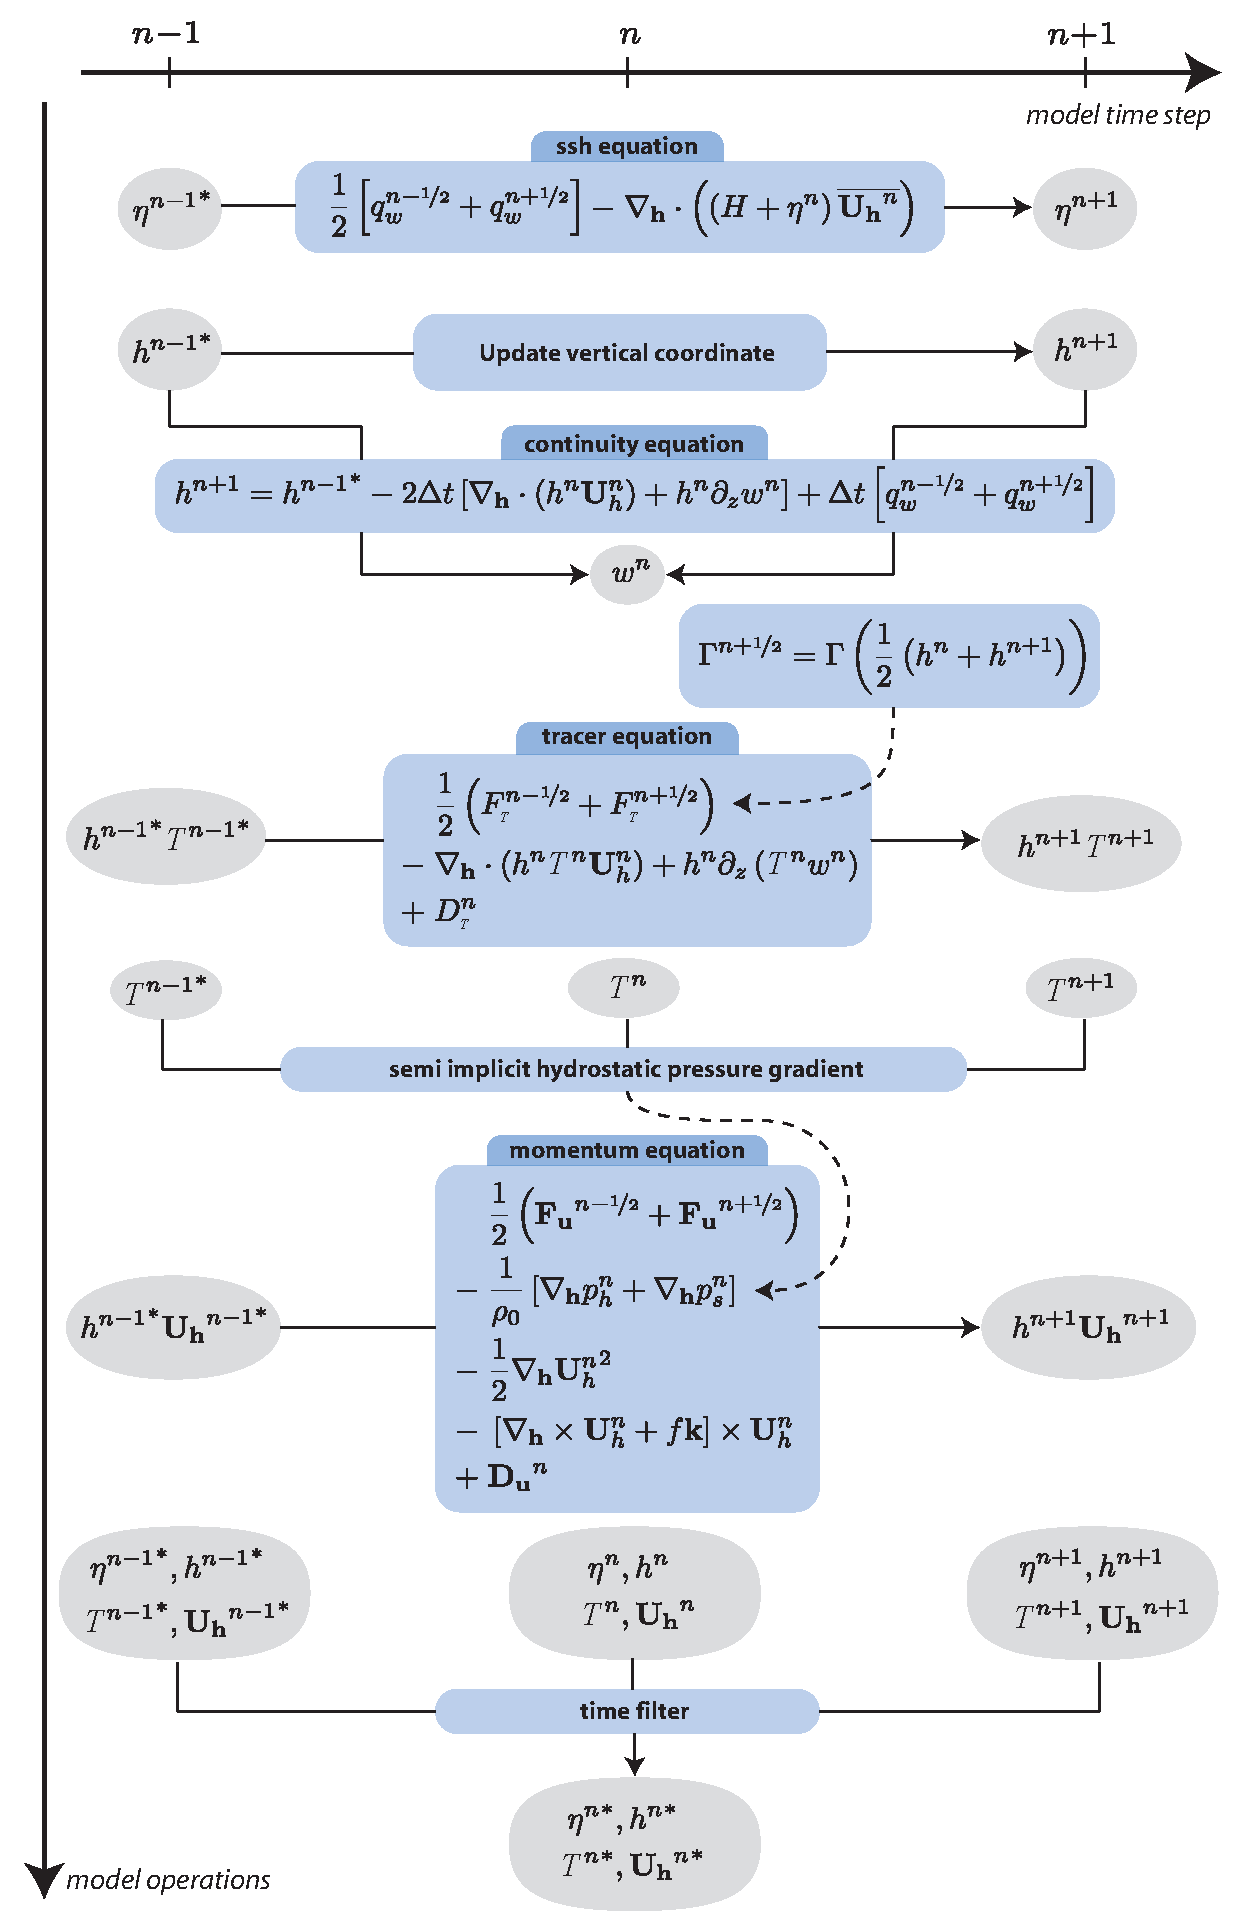
\includegraphics[width=0.7\textwidth]{./TexFiles/Figures/Fig_TimeStepping_flowchart.pdf}
\caption{ 	\label{Fig_TimeStep_flowchart}
Sketch of the leapfrog time stepping sequence in \NEMO from \citet{Leclair_Madec_OM09}. 
The use of a semi-implicit computation of the hydrostatic pressure gradient requires
the tracer equation to be stepped forward prior to the momentum equation. 
The need for knowledge of the vertical scale factor (here denoted as $h$)
requires the sea surface height and the continuity equation to be stepped forward
prior to the computation of the tracer equation.
Note that the method for the evaluation of the surface pressure gradient $\nabla p_s$ is not presented here 
(see \S~\ref{DYN_spg}). }
\end{center}   \end{figure}
%>>>>>>>>>>>>>>>>>>>>>>>>>>>>
%}

The range of stability of the Leap-Frog scheme can be extended by a factor of two
by introducing a semi-implicit computation of the hydrostatic pressure gradient term
\citep{Brown_Campana_MWR78}. Instead of evaluating the pressure at $t$, a linear 
combination of values at $t-\rdt$, $t$ and $t+\rdt$ is used (see \S~\ref{DYN_hpg_imp}).  
This technique, controlled by the \np{nn\_dynhpg\_rst} namelist parameter, does not 
introduce a significant additional computational cost when tracers and thus density 
is time stepped before the dynamics. This time step ordering is used in \NEMO 
(Fig.\ref{Fig_TimeStep_flowchart}).


This technique, used in several GCMs (\NEMO, POP or MOM for instance), 
makes the Leap-Frog scheme as efficient 
\footnote{The efficiency is defined as the maximum allowed Courant number of the time 
stepping scheme divided by the number of computations of the right-hand side per time step.} 
as the Forward-Backward scheme used in MOM \citep{Griffies_al_OS05} and more 
efficient than the LF-AM3 scheme (leapfrog time stepping combined with a third order
Adams-Moulthon interpolation for the predictor phase) used in ROMS 
\citep{Shchepetkin_McWilliams_OM05}. 

In fact, this technique is efficient when the physical phenomenon that 
limits the time-step is internal gravity waves (IGWs). Indeed, it is 
equivalent to applying a time filter to the pressure gradient to eliminate high 
frequency IGWs. Obviously, the doubling of the time-step is achievable only 
if no other factors control the time-step, such as the stability limits associated 
with advection, diffusion or Coriolis terms. For example, it is inefficient in low resolution
global ocean configurations, since inertial oscillations in the vicinity of the North Pole 
are the limiting factor for the time step. It is also often inefficient in very high 
resolution configurations where strong currents and small grid cells exert 
the strongest constraint on the time step.

% -------------------------------------------------------------------------------------------------------------
%        The Modified Leapfrog -- Asselin Filter scheme
% -------------------------------------------------------------------------------------------------------------
\section{The Modified Leapfrog -- Asselin Filter scheme}
\label{STP_mLF}

Significant changes have been introduced by \cite{Leclair_Madec_OM09} in the 
LF-RA scheme in order to ensure tracer conservation and to allow the use of 
a much smaller value of the Asselin filter parameter. The modifications affect 
both the forcing and filtering treatments in the LF-RA scheme.

In a classical LF-RA environment, the forcing term is centred in time, $i.e.$ 
it is time-stepped over a $2\rdt$ period:  $x^t  = x^t + 2\rdt Q^t $ where $Q$ 
is the forcing applied to $x$, and the time filter is given by \eqref{Eq_STP_asselin} 
so that $Q$ is redistributed over several time step. 
In the modified LF-RA environment, these two formulations have been replaced by:
\begin{align} 
x^{t+\rdt}  &= x^{t-\rdt} + \rdt \left( Q^{t-\rdt/2} + Q^{t+\rdt/2} \right)                   \label{Eq_STP_forcing} \\
%
x_F^t  &= x^t + \gamma \, \left[ x_F^{t-\rdt} - 2 x^t + x^{t+\rdt} \right] 
           - \gamma\,\rdt \, \left[ Q^{t+\rdt/2} -  Q^{t-\rdt/2} \right]                          \label{Eq_STP_RA}
\end{align}
The change in the forcing formulation given by \eqref{Eq_STP_forcing} 
(see Fig.\ref{Fig_MLF_forcing}) has a significant effect: the forcing term no 
longer excites the divergence of odd and even time steps \citep{Leclair_Madec_OM09}. 
% forcing seen by the model....
This property improves the LF-RA scheme in two respects. 
First, the LF-RA can now ensure the local and global conservation of tracers.
Indeed, time filtering is no longer required on the forcing part. The influence of 
the Asselin filter on the forcing is be removed by adding a new term in the filter
(last term in \eqref{Eq_STP_RA} compared to \eqref{Eq_STP_asselin}). Since 
the filtering of the forcing was the source of non-conservation in the classical 
LF-RA scheme, the modified formulation becomes conservative  \citep{Leclair_Madec_OM09}.
Second, the LF-RA becomes a truly quasi-second order scheme. Indeed, 
\eqref{Eq_STP_forcing} used in combination with a careful treatment of static 
instability (\S\ref{ZDF_evd}) and of the TKE physics (\S\ref{ZDF_tke_ene}),
the two other main sources of time step divergence, allows a reduction by 
two orders of magnitude of the Asselin filter parameter. 

Note that the forcing is now provided at the middle of a time step: $Q^{t+\rdt/2}$ 
is the forcing applied over the $[t,t+\rdt]$ time interval. This and the change 
in the time filter, \eqref{Eq_STP_RA}, allows an exact evaluation of the 
contribution due to the forcing term between any two time steps, 
even if separated by only $\rdt$ since the time filter is no longer applied to the
forcing term.

%>>>>>>>>>>>>>>>>>>>>>>>>>>>>
\begin{figure}[!t] 	  \begin{center}
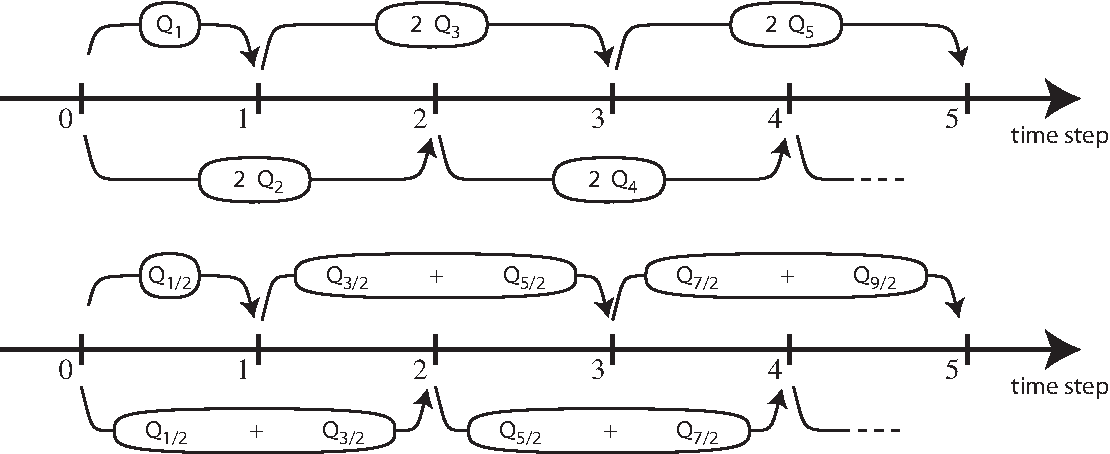
\includegraphics[width=0.90\textwidth]{./TexFiles/Figures/Fig_MLF_forcing.pdf}
\caption{ 	\label{Fig_MLF_forcing}
Illustration of forcing integration methods. 
(top) ''Traditional'' formulation : the forcing is defined at the same time as the variable 
to which it is applied (integer value of the time step index) and it is applied over a $2\rdt$ period. 
(bottom)  modified formulation : the forcing is defined in the middle of the time (integer and a half 
value of the time step index) and the mean of two successive forcing values ($n-1/2$, $n+1/2$).
is applied over a $2\rdt$ period.}
\end{center}   \end{figure}
%>>>>>>>>>>>>>>>>>>>>>>>>>>>>

% -------------------------------------------------------------------------------------------------------------
%        Start/Restart strategy
% -------------------------------------------------------------------------------------------------------------
\section{Start/Restart strategy}
\label{STP_rst}
%--------------------------------------------namrun-------------------------------------------
\namdisplay{namrun}         
%--------------------------------------------------------------------------------------------------------------

The first time step of this three level scheme when starting from initial conditions 
is a forward step (Euler time integration): 
\begin{equation} \label{Eq_DOM_euler}
	x^1 = x^0 + \rdt \ \text{RHS}^0
\end{equation}
This is done simply by keeping the leapfrog environment ($i.e.$ the \eqref{Eq_STP} 
three level time stepping) but setting all $x^0$ (\textit{before}) and $x^{1}$ (\textit{now}) fields 
equal at the first time step and using half the value of $\rdt$.

It is also possible to restart from a previous computation, by using a 
restart file. The restart strategy is designed to ensure perfect 
restartability of the code: the user should obtain the same results to 
machine precision either by running the model for $2N$ time steps in one go, 
or by performing two consecutive experiments of $N$ steps with a restart. 
This requires saving two time levels and many auxiliary data in the restart 
files in machine precision. 

Note that when a semi-implicit scheme is used to evaluate the hydrostatic pressure 
gradient (see \S\ref{DYN_hpg_imp}), an extra three-dimensional field has to be 
added to the restart file to ensure an exact restartability. This is done optionally 
via the  \np{nn\_dynhpg\_rst} namelist parameter, so that the size of the
restart file can be reduced when restartability is not a key issue (operational 
oceanography or in ensemble simulations for seasonal forecasting).

Note the size of the time step used, $\rdt$, is also saved in the restart file. 
When restarting, if the the time step has been changed, a restart using an Euler time 
stepping scheme is imposed. 
Options are defined through the  \ngn{namrun} namelist variables.
%%%
\gmcomment{
add here how to force the restart to contain only one time step for operational purposes

add also the idea of writing several restart for seasonal forecast : how is it done ?

verify that all namelist pararmeters are truly described 

a word on the check of restart  .....
}
%%%

\gmcomment{       % add a subsection here  

%-------------------------------------------------------------------------------------------------------------
%        Time Domain
% -------------------------------------------------------------------------------------------------------------
\subsection{Time domain}
\label{STP_time}
%--------------------------------------------namrun-------------------------------------------
\namdisplay{namdom}         
%--------------------------------------------------------------------------------------------------------------

Options are defined through the  \ngn{namdom} namelist variables.
 \colorbox{yellow}{add here a few word on nit000 and nitend}

 \colorbox{yellow}{Write documentation on the calendar and the key variable adatrj}

add a description of daymod, and the model calandar (leap-year and co)

}     	%% end add



%%
\gmcomment{       % add implicit in vvl case  and Crant-Nicholson scheme   

Implicit time stepping in case of variable volume thickness.

Tracer case (NB for momentum in vector invariant form take care!)

\begin{flalign*}
&\frac{\left( e_{3t}\,T \right)_k^{t+1}-\left( e_{3t}\,T \right)_k^{t-1}}{2\rdt}
\equiv \text{RHS}+ \delta _k \left[ {\frac{A_w^{vt} }{e_{3w}^{t+1} }\delta _{k+1/2} \left[ {T^{t+1}} \right]} 
\right]      \\
&\left( e_{3t}\,T \right)_k^{t+1}-\left( e_{3t}\,T \right)_k^{t-1}
\equiv {2\rdt} \ \text{RHS}+ {2\rdt} \ \delta _k \left[ {\frac{A_w^{vt} }{e_{3w}^{t+1} }\delta _{k+1/2} \left[ {T^{t+1}} \right]} 
\right]      \\
&\left( e_{3t}\,T \right)_k^{t+1}-\left( e_{3t}\,T \right)_k^{t-1}
\equiv 2\rdt \ \text{RHS}
+ 2\rdt \ \left\{ \left[ \frac{A_w^{vt}}{e_{3w}^{t+1}} \right]_{k+1/2} [ T_{k+1}^{t+1} - T_k      ^{t+1} ]
                          - \left[ \frac{A_w^{vt}}{e_{3w}^{t+1}} \right]_{k-1/2} [ T_k       ^{t+1} - T_{k-1}^{t+1} ]  \right\}     \\
&\\
&\left( e_{3t}\,T \right)_k^{t+1}
-  {2\rdt} \           \left[ \frac{A_w^{vt}}{e_{3w}^{t+1}} \right]_{k+1/2}                  T_{k+1}^{t+1} 
+ {2\rdt} \ \left\{  \left[ \frac{A_w^{vt}}{e_{3w}^{t+1}} \right]_{k+1/2} 
                            +  \left[ \frac{A_w^{vt}}{e_{3w}^{t+1}} \right]_{k-1/2}     \right\}   T_{k    }^{t+1}
-  {2\rdt} \           \left[ \frac{A_w^{vt}}{e_{3w}^{t+1}} \right]_{k-1/2}                  T_{k-1}^{t+1}      \\
&\equiv \left( e_{3t}\,T \right)_k^{t-1} + {2\rdt} \ \text{RHS}    \\
%
\end{flalign*}

\begin{flalign*}
\allowdisplaybreaks
\intertext{ Tracer case }
%
&  \qquad \qquad  \quad   -  {2\rdt}                  \ \left[ \frac{A_w^{vt}}{e_{3w}^{t+1}} \right]_{k+1/2}   
                                                                                                      \qquad \qquad \qquad  \qquad  T_{k+1}^{t+1}   \\
&+ {2\rdt} \ \biggl\{  (e_{3t})_{k   }^{t+1}  \bigg. +    \left[ \frac{A_w^{vt}}{e_{3w}^{t+1}} \right]_{k+1/2}  
                                                                               +   \left[ \frac{A_w^{vt}}{e_{3w}^{t+1}} \right]_{k-1/2} \bigg. \biggr\}  \ \ \ T_{k   }^{t+1}  &&\\
& \qquad \qquad  \qquad \qquad \qquad \quad \ \ -  {2\rdt} \                          \left[ \frac{A_w^{vt}}{e_{3w}^{t+1}} \right]_{k-1/2}                          \quad \ \ T_{k-1}^{t+1}     
\ \equiv \ \left( e_{3t}\,T \right)_k^{t-1} + {2\rdt} \ \text{RHS}  \\
%
\end{flalign*}
\begin{flalign*}
\allowdisplaybreaks
\intertext{ Tracer content case }
%
& -  {2\rdt} \              & \frac{(A_w^{vt})_{k+1/2}} {(e_{3w})_{k+1/2}^{t+1}\;(e_{3t})_{k+1}^{t+1}}  && \  \left( e_{3t}\,T \right)_{k+1}^{t+1}   &\\
& + {2\rdt} \ \left[ 1  \right.+ & \frac{(A_w^{vt})_{k+1/2}} {(e_{3w})_{k+1/2}^{t+1}\;(e_{3t})_k^{t+1}} 
                                    + & \frac{(A_w^{vt})_{k -1/2}} {(e_{3w})_{k -1/2}^{t+1}\;(e_{3t})_k^{t+1}}  \left.  \right]  & \left( e_{3t}\,T \right)_{k   }^{t+1}  &\\
& -  {2\rdt} \               & \frac{(A_w^{vt})_{k -1/2}} {(e_{3w})_{k -1/2}^{t+1}\;(e_{3t})_{k-1}^{t+1}}     &\  \left( e_{3t}\,T \right)_{k-1}^{t+1}   
\equiv \left( e_{3t}\,T \right)_k^{t-1} + {2\rdt} \ \text{RHS}  &
\end{flalign*}

%%
}
%%
			% Time discretisation (time stepping strategy)

% ================================================================
% Chapter 2 � Space and Time Domain (DOM)
% ================================================================
\chapter{Space Domain (DOM) }
\label{DOM}
\minitoc

% Missing things:
% 	- istate: description of the initial state   ==> this has to be put elsewhere..
%                  perhaps in MISC ?  By the way the initialisation of T S and dynamics 
%                  should be put outside of DOM routine (better with TRC staff and off-line
%                  tracers)
% 	-geo2ocean:  how to switch from geographic to mesh coordinate
%     - domclo:  closed sea and lakes.... management of closea sea area : specific to global configuration, both forced and coupled


\newpage
$\ $\newline    % force a new ligne

Having defined the continuous equations in Chap.~\ref{PE} and chosen a time 
discretization Chap.~\ref{STP}, we need to choose a discretization on a grid, 
and numerical algorithms. In the present chapter, we provide a general description 
of the staggered grid used in \NEMO, and other information relevant to the main 
directory routines as well as the DOM (DOMain) directory. 

$\ $\newline    % force a new lign

% ================================================================
% Fundamentals of the Discretisation
% ================================================================
\section{Fundamentals of the Discretisation}
\label{DOM_basics}

% -------------------------------------------------------------------------------------------------------------
%        Arrangement of Variables 
% -------------------------------------------------------------------------------------------------------------
\subsection{Arrangement of Variables}
\label{DOM_cell}

%>>>>>>>>>>>>>>>>>>>>>>>>>>>>
\begin{figure}[!tb]    \begin{center}
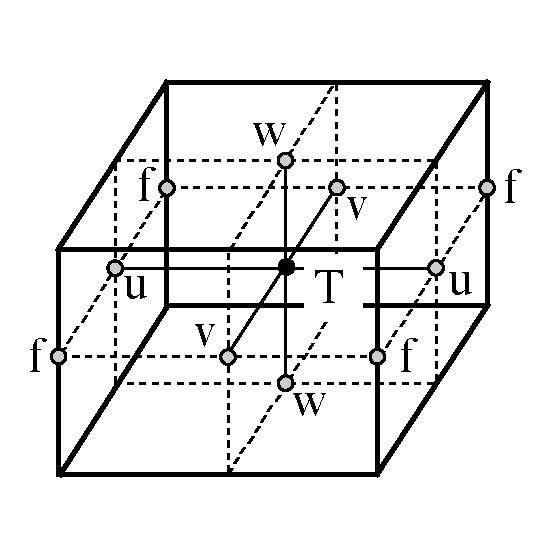
\includegraphics[width=0.90\textwidth]{./TexFiles/Figures/Fig_cell.pdf}
\caption{ \label{Fig_cell}    
Arrangement of variables. $t$ indicates scalar points where temperature, 
salinity, density, pressure and horizontal divergence are defined. ($u$,$v$,$w$) 
indicates vector points, and $f$ indicates vorticity points where both relative and 
planetary vorticities are defined}
\end{center}   \end{figure}
%>>>>>>>>>>>>>>>>>>>>>>>>>>>>

The numerical techniques used to solve the Primitive Equations in this model are 
based on the traditional, centred second-order finite difference approximation. 
Special attention has been given to the homogeneity of the solution in the three 
space directions. The arrangement of variables is the same in all directions. 
It consists of cells centred on scalar points ($t$, $S$, $p$, $\rho$) with vector 
points $(u, v, w)$ defined in the centre of each face of the cells (Fig. \ref{Fig_cell}). 
This is the generalisation to three dimensions of the well-known ``C'' grid in 
Arakawa's classification \citep{Mesinger_Arakawa_Bk76}. The relative and 
planetary vorticity, $\zeta$ and $f$, are defined in the centre of each vertical edge 
and the barotropic stream function $\psi$ is defined at horizontal points overlying 
the $\zeta$ and $f$-points.

The ocean mesh ($i.e.$ the position of all the scalar and vector points) is defined 
by the transformation that gives ($\lambda$ ,$\varphi$ ,$z$) as a function of $(i,j,k)$. 
The grid-points are located at integer or integer and a half value of $(i,j,k)$ as 
indicated on Table \ref{Tab_cell}. In all the following, subscripts $u$, $v$, $w$, 
$f$, $uw$, $vw$ or $fw$ indicate the position of the grid-point where the scale 
factors are defined. Each scale factor is defined as the local analytical value 
provided by \eqref{Eq_scale_factors}. As a result, the mesh on which partial 
derivatives $\frac{\partial}{\partial \lambda}, \frac{\partial}{\partial \varphi}$, and 
$\frac{\partial}{\partial z} $ are evaluated is a uniform mesh with a grid size of unity. 
Discrete partial derivatives are formulated by the traditional, centred second order 
finite difference approximation while the scale factors are chosen equal to their 
local analytical value. An important point here is that the partial derivative of the 
scale factors must be evaluated by centred finite difference approximation, not 
from their analytical expression. This preserves the symmetry of the discrete set 
of equations and therefore satisfies many of the continuous properties (see 
Appendix~\ref{Apdx_C}). A similar, related remark can be made about the domain 
size: when needed, an area, volume, or the total ocean depth must be evaluated 
as the sum of the relevant scale factors (see \eqref{DOM_bar}) in the next section). 

%>>>>>>>>>>>>>>>>>>>>>>>>>>>>
\begin{table}[!tb]
\begin{center} \begin{tabular}{|p{46pt}|p{56pt}|p{56pt}|p{56pt}|}
\hline
T	&$i$ 		& $j$		& $k$		 \\ \hline
u	& $i+1/2$	& $j$		& $k$	 	\\ \hline
v	& $i$	 	& $j+1/2$	& $k$	 	\\ \hline
w	& $i$	 	& $j$		& $k+1/2$ 	\\ \hline
f	& $i+1/2$ 	& $j+1/2$	& $k$	 	\\ \hline
uw	& $i+1/2$ 	& $j$		& $k+1/2$ 	\\ \hline
vw	& $i$	 	& $j+1/2$	& $k+1/2$ 	\\ \hline
fw	& $i+1/2$ 	& $j+1/2$	& $k+1/2$ 	\\ \hline
\end{tabular}
\caption{ \label{Tab_cell}
Location of grid-points as a function of integer or integer and a half value of the column, 
line or level. This indexing is only used for the writing of the semi-discrete equation. 
In the code, the indexing uses integer values only and has a reverse direction 
in the vertical (see \S\ref{DOM_Num_Index})}
\end{center}
\end{table}
%>>>>>>>>>>>>>>>>>>>>>>>>>>>>

% -------------------------------------------------------------------------------------------------------------
%        Vector Invariant Formulation 
% -------------------------------------------------------------------------------------------------------------
\subsection{Discrete Operators}
\label{DOM_operators}

Given the values of a variable $q$ at adjacent points, the differencing and 
averaging operators at the midpoint between them are:
\begin{subequations} \label{Eq_di_mi}
\begin{align}
 \delta _i [q]       &=  \  \    q(i+1/2)  - q(i-1/2)		\\
 \overline q^{\,i} &= \left\{ q(i+1/2) + q(i-1/2) \right\} \; / \; 2
\end{align}
\end{subequations}

Similar operators are defined with respect to $i+1/2$, $j$, $j+1/2$, $k$, and 
$k+1/2$. Following \eqref{Eq_PE_grad} and \eqref{Eq_PE_lap}, the gradient of a 
variable $q$ defined at a $t$-point has its three components defined at $u$-, $v$- 
and $w$-points while its Laplacien is defined at $t$-point. These operators have 
the following discrete forms in the curvilinear $s$-coordinate system:
\begin{equation} \label{Eq_DOM_grad}
\nabla q\equiv 	\frac{1}{e_{1u} } \delta _{i+1/2 } [q] \;\,\mathbf{i}
		+	\frac{1}{e_{2v} } \delta _{j+1/2 } [q] \;\,\mathbf{j}
		+	\frac{1}{e_{3w}} \delta _{k+1/2} [q] \;\,\mathbf{k}
\end{equation}
\begin{multline} \label{Eq_DOM_lap}
\Delta q\equiv \frac{1}{e_{1t}\,e_{2t}\,e_{3t} }
       \;\left(          \delta_i  \left[ \frac{e_{2u}\,e_{3u}} {e_{1u}} \;\delta_{i+1/2} [q] \right]
+                        \delta_j  \left[ \frac{e_{1v}\,e_{3v}}  {e_{2v}} \;\delta_{j+1/2} [q] \right] \;  \right)		\\
+\frac{1}{e_{3t}} \delta_k \left[ \frac{1}{e_{3w} }                     \;\delta_{k+1/2} [q] \right]
\end{multline}

Following \eqref{Eq_PE_curl} and \eqref{Eq_PE_div}, a vector ${\rm {\bf A}}=\left( a_1,a_2,a_3\right)$ 
defined at vector points $(u,v,w)$ has its three curl components defined at $vw$-, $uw$, 
and $f$-points, and its divergence defined at $t$-points:
\begin{eqnarray}  \label{Eq_DOM_curl}
 \nabla \times {\rm {\bf A}}\equiv &
      \frac{1}{e_{2v}\,e_{3vw} } \ \left( \delta_{j +1/2} \left[e_{3w}\,a_3 \right] -\delta_{k+1/2} \left[e_{2v} \,a_2 \right] \right)  &\ \mathbf{i} \\ 
 +& \frac{1}{e_{2u}\,e_{3uw}} \ \left( \delta_{k+1/2} \left[e_{1u}\,a_1  \right] -\delta_{i +1/2} \left[e_{3w}\,a_3 \right] \right)  &\ \mathbf{j} \\
 +& \frac{1}{e_{1f} \,e_{2f}    } \ \left( \delta_{i +1/2} \left[e_{2v}\,a_2  \right] -\delta_{j +1/2} \left[e_{1u}\,a_1 \right] \right)  &\ \mathbf{k}
 \end{eqnarray}
\begin{equation} \label{Eq_DOM_div}
\nabla \cdot \rm{\bf A}=\frac{1}{e_{1t}\,e_{2t}\,e_{3t}}\left( \delta_i \left[e_{2u}\,e_{3u}\,a_1 \right]
                                                                                         +\delta_j \left[e_{1v}\,e_{3v}\,a_2 \right] \right)+\frac{1}{e_{3t} }\delta_k \left[a_3 \right]
\end{equation}

In the special case of a pure $z$-coordinate system, \eqref{Eq_DOM_lap} and 
\eqref{Eq_DOM_div} can be simplified. In this case, the vertical scale factor 
becomes a function of the single variable $k$ and thus does not depend on the 
horizontal location of a grid point. For example \eqref{Eq_DOM_div} reduces to: 
\begin{equation*}
\nabla \cdot \rm{\bf A}=\frac{1}{e_{1t}\,e_{2t}} \left( \delta_i \left[e_{2u}\,a_1 \right] 
                                                                              +\delta_j \left[e_{1v}\, a_2 \right]  \right)
                                                     +\frac{1}{e_{3t}} \delta_k \left[             a_3 \right]
\end{equation*}

The vertical average over the whole water column denoted by an overbar becomes 
for a quantity $q$ which is a masked field (i.e. equal to zero inside solid area):
\begin{equation} \label{DOM_bar}
\bar q 	=         \frac{1}{H}    \int_{k^b}^{k^o} {q\;e_{3q} \,dk} 
		\equiv \frac{1}{H_q }\sum\limits_k {q\;e_{3q} }
\end{equation}
where $H_q$  is the ocean depth, which is the masked sum of the vertical scale 
factors at $q$ points, $k^b$ and $k^o$ are the bottom and surface $k$-indices, 
and the symbol $k^o$ refers to a summation over all grid points of the same type 
in the direction indicated by the subscript (here $k$). 

In continuous form, the following properties are satisfied:
\begin{equation} \label{Eq_DOM_curl_grad}
\nabla \times \nabla q ={\rm {\bf {0}}}
\end{equation}
\begin{equation} \label{Eq_DOM_div_curl}
\nabla \cdot \left( {\nabla \times {\rm {\bf A}}} \right)=0
\end{equation}

It is straightforward to demonstrate that these properties are verified locally in 
discrete form as soon as the scalar $q$ is taken at $t$-points and the vector 
\textbf{A} has its components defined at vector points $(u,v,w)$.

Let $a$ and $b$ be two fields defined on the mesh, with value zero inside 
continental area. Using integration by parts it can be shown that the differencing 
operators ($\delta_i$, $\delta_j$ and $\delta_k$) are anti-symmetric linear 
operators, and further that the averaging operators $\overline{\,\cdot\,}^{\,i}$, 
$\overline{\,\cdot\,}^{\,k}$ and $\overline{\,\cdot\,}^{\,k}$) are symmetric linear 
operators, $i.e.$
\begin{align} 
\label{DOM_di_adj}
\sum\limits_i { a_i \;\delta _i \left[ b \right]} 
	&\equiv -\sum\limits_i {\delta _{i+1/2} \left[ a \right]\;b_{i+1/2} }      \\
\label{DOM_mi_adj}
\sum\limits_i { a_i \;\overline b^{\,i}} 
	& \equiv \quad \sum\limits_i {\overline a ^{\,i+1/2}\;b_{i+1/2} } 
\end{align}

In other words, the adjoint of the differencing and averaging operators are 
$\delta_i^*=\delta_{i+1/2}$ and 
${(\overline{\,\cdot \,}^{\,i})}^*= \overline{\,\cdot\,}^{\,i+1/2}$, respectively. 
These two properties will be used extensively in the Appendix~\ref{Apdx_C} to 
demonstrate integral conservative properties of the discrete formulation chosen.

% -------------------------------------------------------------------------------------------------------------
%        Numerical Indexing 
% -------------------------------------------------------------------------------------------------------------
\subsection{Numerical Indexing}
\label{DOM_Num_Index}

%>>>>>>>>>>>>>>>>>>>>>>>>>>>>
\begin{figure}[!tb]  \begin{center}
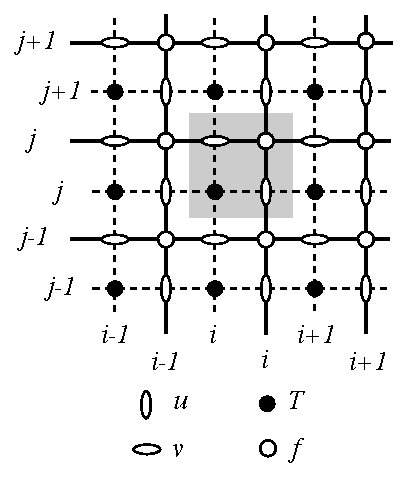
\includegraphics[width=0.90\textwidth]{./TexFiles/Figures/Fig_index_hor.pdf}
\caption{   \label{Fig_index_hor}    
Horizontal integer indexing used in the \textsc{Fortran} code. The dashed area indicates 
the cell in which variables contained in arrays have the same $i$- and $j$-indices}
\end{center}   \end{figure}
%>>>>>>>>>>>>>>>>>>>>>>>>>>>>

The array representation used in the \textsc{Fortran} code requires an integer 
indexing while the analytical definition of the mesh (see \S\ref{DOM_cell}) is 
associated with the use of integer values for $t$-points and both integer and 
integer and a half values for all the other points. Therefore a specific integer 
indexing must be defined for points other than $t$-points ($i.e.$ velocity and 
vorticity grid-points). Furthermore, the direction of the vertical indexing has 
been changed so that the surface level is at $k=1$.

% -----------------------------------
%        Horizontal Indexing 
% -----------------------------------
\subsubsection{Horizontal Indexing}
\label{DOM_Num_Index_hor}

The indexing in the horizontal plane has been chosen as shown in Fig.\ref{Fig_index_hor}. 
For an increasing $i$ index ($j$ index), the $t$-point and the eastward $u$-point 
(northward $v$-point) have the same index (see the dashed area in Fig.\ref{Fig_index_hor}). 
A $t$-point and its nearest northeast $f$-point have the same $i$-and $j$-indices.

% -----------------------------------
%        Vertical indexing 
% -----------------------------------
\subsubsection{Vertical Indexing}
\label{DOM_Num_Index_vertical}

In the vertical, the chosen indexing requires special attention since the 
$k$-axis is re-orientated downward in the \textsc{Fortran} code compared 
to the indexing used in the semi-discrete equations and given in \S\ref{DOM_cell}. 
The sea surface corresponds to the $w$-level $k=1$ which is the same index 
as $t$-level just below (Fig.\ref{Fig_index_vert}). The last $w$-level ($k=jpk$) 
either corresponds to the ocean floor or is inside the bathymetry while the last 
$t$-level is always inside the bathymetry (Fig.\ref{Fig_index_vert}). Note that 
for an increasing $k$ index, a $w$-point and the $t$-point just below have the 
same $k$ index, in opposition to what is done in the horizontal plane where 
it is the $t$-point and the nearest velocity points in the direction of the horizontal 
axis that have the same $i$ or $j$ index (compare the dashed area in 
Fig.\ref{Fig_index_hor} and \ref{Fig_index_vert}). Since the scale factors are 
chosen to be strictly positive, a \emph{minus sign} appears in the \textsc{Fortran} 
code \emph{before all the vertical derivatives} of the discrete equations given in 
this documentation.

%>>>>>>>>>>>>>>>>>>>>>>>>>>>>
\begin{figure}[!pt]    \begin{center}
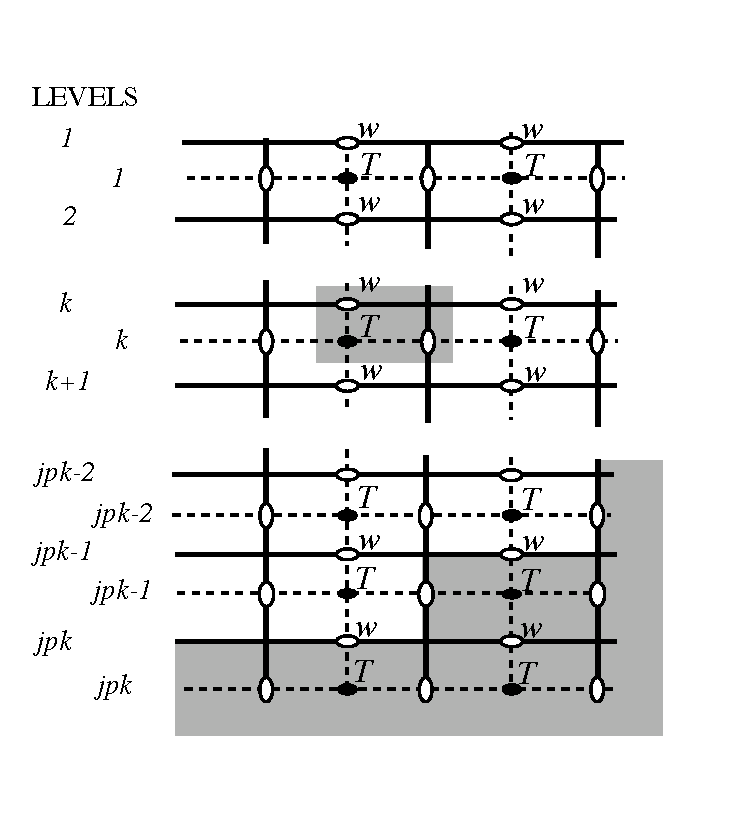
\includegraphics[width=.90\textwidth]{./TexFiles/Figures/Fig_index_vert.pdf}
\caption{ \label{Fig_index_vert}     
Vertical integer indexing used in the \textsc{Fortran } code. Note that 
the $k$-axis is orientated downward. The dashed area indicates the cell in 
which variables contained in arrays have the same $k$-index.}
\end{center}   \end{figure}
%>>>>>>>>>>>>>>>>>>>>>>>>>>>>

% -----------------------------------
%        Domain Size
% -----------------------------------
\subsubsection{Domain Size}
\label{DOM_size}

The total size of the computational domain is set by the parameters \np{jpiglo}, 
\np{jpjglo} and \np{jpkdta} in the $i$, $j$ and $k$ directions respectively. They are 
given as namelist variables in the \ngn{namcfg} namelist. 

Note that are other namelist variables in the \ngn{namcfg} namelist that refer to
 the domain size. 
The two variables \np{jpidta} and \np{jpjdta} may be larger than \np{jpiglo}, \np{jpjglo}
when the user wants to use only a sub-region of a given configuration. This is 
the "zoom" capability described in \S\ref{MISC_zoom}. In most applications of 
the model, $jpidta=jpiglo$, $jpjdta=jpjglo$, and $jpizoom=jpjzoom=1$. Parameters 
$jpi$ and $jpj$ refer to the size of each processor subdomain when the code is 
run in parallel using domain decomposition (\key{mpp\_mpi} defined, see 
\S\ref{LBC_mpp}).


$\ $\newline    % force a new lign

% ================================================================
% Domain: Horizontal Grid (mesh) 
% ================================================================
\section  [Domain: Horizontal Grid (mesh) (\textit{domhgr})]               
		{Domain: Horizontal Grid (mesh) \small{(\mdl{domhgr} module)} }
\label{DOM_hgr}

% -------------------------------------------------------------------------------------------------------------
%        Coordinates and scale factors 
% -------------------------------------------------------------------------------------------------------------
\subsection{Coordinates and scale factors}
\label{DOM_hgr_coord_e}

The ocean mesh ($i.e.$ the position of all the scalar and vector points) is defined 
by the transformation that gives $(\lambda,\varphi,z)$ as a function of $(i,j,k)$. 
The grid-points are located at integer or integer and a half values of as indicated 
in Table~\ref{Tab_cell}. The associated scale factors are defined using the 
analytical first derivative of the transformation \eqref{Eq_scale_factors}. These 
definitions are done in two modules, \mdl{domhgr} and \mdl{domzgr}, which 
provide the horizontal and vertical meshes, respectively. This section deals with 
the horizontal mesh parameters.

In a horizontal plane, the location of all the model grid points is defined from the 
analytical expressions of the longitude $\lambda$ and  latitude $\varphi$ as a 
function of  $(i,j)$. The horizontal scale factors are calculated using 
\eqref{Eq_scale_factors}. For example, when the longitude and latitude are 
function of a single value ($i$ and $j$, respectively) (geographical configuration 
of the mesh), the horizontal mesh definition reduces to define the wanted 
$\lambda(i)$, $\varphi(j)$, and their derivatives $\lambda'(i)$ $\varphi'(j)$ in the 
\mdl{domhgr} module. The model computes the grid-point positions and scale 
factors in the horizontal plane as follows:
\begin{flalign*}
\lambda_t &\equiv \text{glamt}= \lambda(i)	  & \varphi_t &\equiv \text{gphit} = \varphi(j)\\
\lambda_u &\equiv \text{glamu}= \lambda(i+1/2)& \varphi_u &\equiv \text{gphiu}= \varphi(j)\\
\lambda_v &\equiv \text{glamv}= \lambda(i)       & \varphi_v &\equiv \text{gphiv} = \varphi(j+1/2)\\
\lambda_f &\equiv \text{glamf }= \lambda(i+1/2)& \varphi_f &\equiv \text{gphif }= \varphi(j+1/2) 
\end{flalign*}
\begin{flalign*}
e_{1t} &\equiv \text{e1t} = r_a |\lambda'(i)		\; \cos\varphi(j)  |&
e_{2t} &\equiv \text{e2t} = r_a |\varphi'(j)|  \\
e_{1u} &\equiv \text{e1t} = r_a |\lambda'(i+1/2)	\; \cos\varphi(j)  |&
e_{2u} &\equiv \text{e2t} = r_a |\varphi'(j)|\\
e_{1v} &\equiv \text{e1t} = r_a |\lambda'(i)		\; \cos\varphi(j+1/2)  |&
e_{2v} &\equiv \text{e2t} = r_a |\varphi'(j+1/2)|\\
e_{1f} &\equiv \text{e1t} = r_a |\lambda'(i+1/2)\; \cos\varphi(j+1/2)  |&
e_{2f} &\equiv \text{e2t} = r_a |\varphi'(j+1/2)|
\end{flalign*}
where the last letter of each computational name indicates the grid point 
considered and $r_a$ is the earth radius (defined in \mdl{phycst} along with 
all universal constants). Note that the horizontal position of and scale factors 
at $w$-points are exactly equal to those of $t$-points, thus no specific arrays 
are defined at $w$-points. 

Note that the definition of the scale factors ($i.e.$ as the analytical first derivative 
of the transformation that gives $(\lambda,\varphi,z)$ as a function of $(i,j,k)$) is 
specific to the \NEMO model \citep{Marti_al_JGR92}. As an example, $e_{1t}$ is defined 
locally at a $t$-point, whereas many other models on a C grid choose to define 
such a scale factor as the distance between the $U$-points on each side of the 
$t$-point. Relying on an analytical transformation has two advantages: firstly, there 
is no ambiguity in the scale factors appearing in the discrete equations, since they 
are first introduced in the continuous equations; secondly, analytical transformations 
encourage good practice by the definition of smoothly varying grids (rather than 
allowing the user to set arbitrary jumps in thickness between adjacent layers) 
\citep{Treguier1996}. An example of the effect of such a choice is shown in 
Fig.~\ref{Fig_zgr_e3}.
%>>>>>>>>>>>>>>>>>>>>>>>>>>>>
\begin{figure}[!t]     \begin{center}
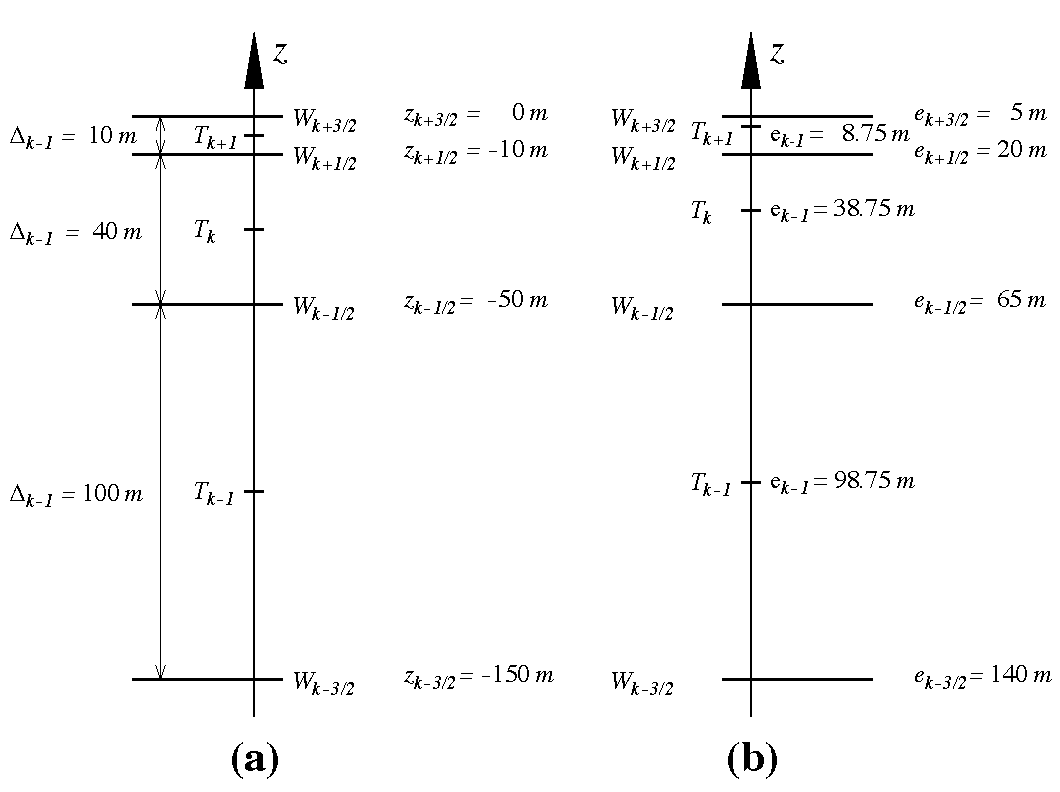
\includegraphics[width=0.90\textwidth]{./TexFiles/Figures/Fig_zgr_e3.pdf}
\caption{ \label{Fig_zgr_e3}    
Comparison of (a) traditional definitions of grid-point position and grid-size in the vertical, 
and (b) analytically derived grid-point position and scale factors. 
For both grids here,  the same $w$-point depth has been chosen but in (a) the 
$t$-points are set half way between $w$-points while in (b) they are defined from 
an analytical function: $z(k)=5\,(i-1/2)^3 - 45\,(i-1/2)^2 + 140\,(i-1/2) - 150$. 
Note the resulting difference between the value of the grid-size $\Delta_k$ and 
those of the scale factor $e_k$. }
\end{center}   \end{figure}
%>>>>>>>>>>>>>>>>>>>>>>>>>>>>

% -------------------------------------------------------------------------------------------------------------
%        Choice of horizontal grid
% -------------------------------------------------------------------------------------------------------------
\subsection{Choice of horizontal grid}
\label{DOM_hgr_msh_choice}

The user has three options available in defining a horizontal grid, which involve 
the namelist variable \np{jphgr\_mesh} of the \ngn{namcfg} namelist. 
\begin{description}
\item[\np{jphgr\_mesh}=0]  The most general curvilinear orthogonal grids.
The coordinates and their first derivatives with respect to $i$ and $j$ are provided
in a input file (\ifile{coordinates}), read in \rou{hgr\_read} subroutine of the domhgr module.
\item[\np{jphgr\_mesh}=1 to 5] A few simple analytical grids are provided (see below). 
For other analytical grids, the \mdl{domhgr} module must be modified by the user. 
\end{description}

There are two simple cases of geographical grids on the sphere. With 
\np{jphgr\_mesh}=1, the grid (expressed in degrees) is regular in space, 
with grid sizes specified by parameters \np{ppe1\_deg} and \np{ppe2\_deg}, 
respectively. Such a geographical grid can be very anisotropic at high latitudes 
because of the convergence of meridians (the zonal scale factors $e_1$ 
become much smaller than the meridional scale factors $e_2$). The Mercator 
grid (\np{jphgr\_mesh}=4) avoids this anisotropy by refining the meridional scale 
factors in the same way as the zonal ones. In this case, meridional scale factors 
and latitudes are calculated analytically using the formulae appropriate for 
a Mercator projection, based on \np{ppe1\_deg} which is a reference grid spacing 
at the equator (this applies even when the geographical equator is situated outside 
the model domain). 
%%%
\gmcomment{ give here the analytical expression of the Mercator mesh}
%%%
In these two cases (\np{jphgr\_mesh}=1 or 4), the grid position is defined by the 
longitude and latitude of the south-westernmost point (\np{ppglamt0} 
and \np{ppgphi0}). Note that for the Mercator grid the user need only provide 
an approximate starting latitude: the real latitude will be recalculated analytically, 
in order to ensure that the equator corresponds to line passing through $t$- 
and $u$-points.  

Rectangular grids ignoring the spherical geometry are defined with 
\np{jphgr\_mesh} = 2, 3, 5. The domain is either an $f$-plane (\np{jphgr\_mesh} = 2, 
Coriolis factor is constant) or a beta-plane (\np{jphgr\_mesh} = 3, the Coriolis factor 
is linear in the $j$-direction). The grid size is uniform in meter in each direction, 
and given by the parameters \np{ppe1\_m} and \np{ppe2\_m} respectively. 
The zonal grid coordinate (\textit{glam} arrays) is in kilometers, starting at zero 
with the first $t$-point. The meridional coordinate (gphi. arrays) is in kilometers, 
and the second $t$-point corresponds to coordinate $gphit=0$. The input 
variable \np{ppglam0} is ignored. \np{ppgphi0} is used to set the reference 
latitude for computation of the Coriolis parameter. In the case of the beta plane, 
\np{ppgphi0} corresponds to the center of the domain. Finally, the special case 
\np{jphgr\_mesh}=5 corresponds to a beta plane in a rotated domain for the 
GYRE configuration, representing a classical mid-latitude double gyre system. 
The rotation allows us to maximize the jet length relative to the gyre areas 
(and the number of grid points). 

The choice of the grid must be consistent with the boundary conditions specified 
by the parameter \np{jperio} (see {\S\ref{LBC}).

% -------------------------------------------------------------------------------------------------------------
%        Grid files
% -------------------------------------------------------------------------------------------------------------
\subsection{Output Grid files}
\label{DOM_hgr_files}

All the arrays relating to a particular ocean model configuration (grid-point 
position, scale factors, masks) can be saved in files if $\np{nn\_msh} \not= 0$ 
(namelist variable in \ngn{namdom}). This can be particularly useful for plots and off-line 
diagnostics. In some cases, the user may choose to make a local modification 
of a scale factor in the code. This is the case in global configurations when 
restricting the width of a specific strait (usually a one-grid-point strait that 
happens to be too wide due to insufficient model resolution). An example 
is Gibraltar Strait in the ORCA2 configuration. When such modifications are done, 
the output grid written when $\np{nn\_msh} \not=0$ is no more equal to the input grid.

$\ $\newline    % force a new lign

% ================================================================
% Domain: Vertical Grid (domzgr)
% ================================================================
\section  [Domain: Vertical Grid (\textit{domzgr})]
		{Domain: Vertical Grid \small{(\mdl{domzgr} module)} }
\label{DOM_zgr}
%-----------------------------------------nam_zgr & namdom-------------------------------------------
\namdisplay{namzgr} 
\namdisplay{namdom} 
%-------------------------------------------------------------------------------------------------------------

Variables are defined through the \ngn{namzgr} and \ngn{namdom} namelists.
In the vertical, the model mesh is determined by four things: 
(1) the bathymetry given in meters ; 
(2) the number of levels of the model (\jp{jpk}) ; 
(3) the analytical transformation $z(i,j,k)$ and the vertical scale factors 
(derivatives of the transformation) ; 
and (4) the masking system, $i.e.$ the number of wet model levels at each 
$(i,j)$ column of points.

%>>>>>>>>>>>>>>>>>>>>>>>>>>>>
\begin{figure}[!tb]    \begin{center}
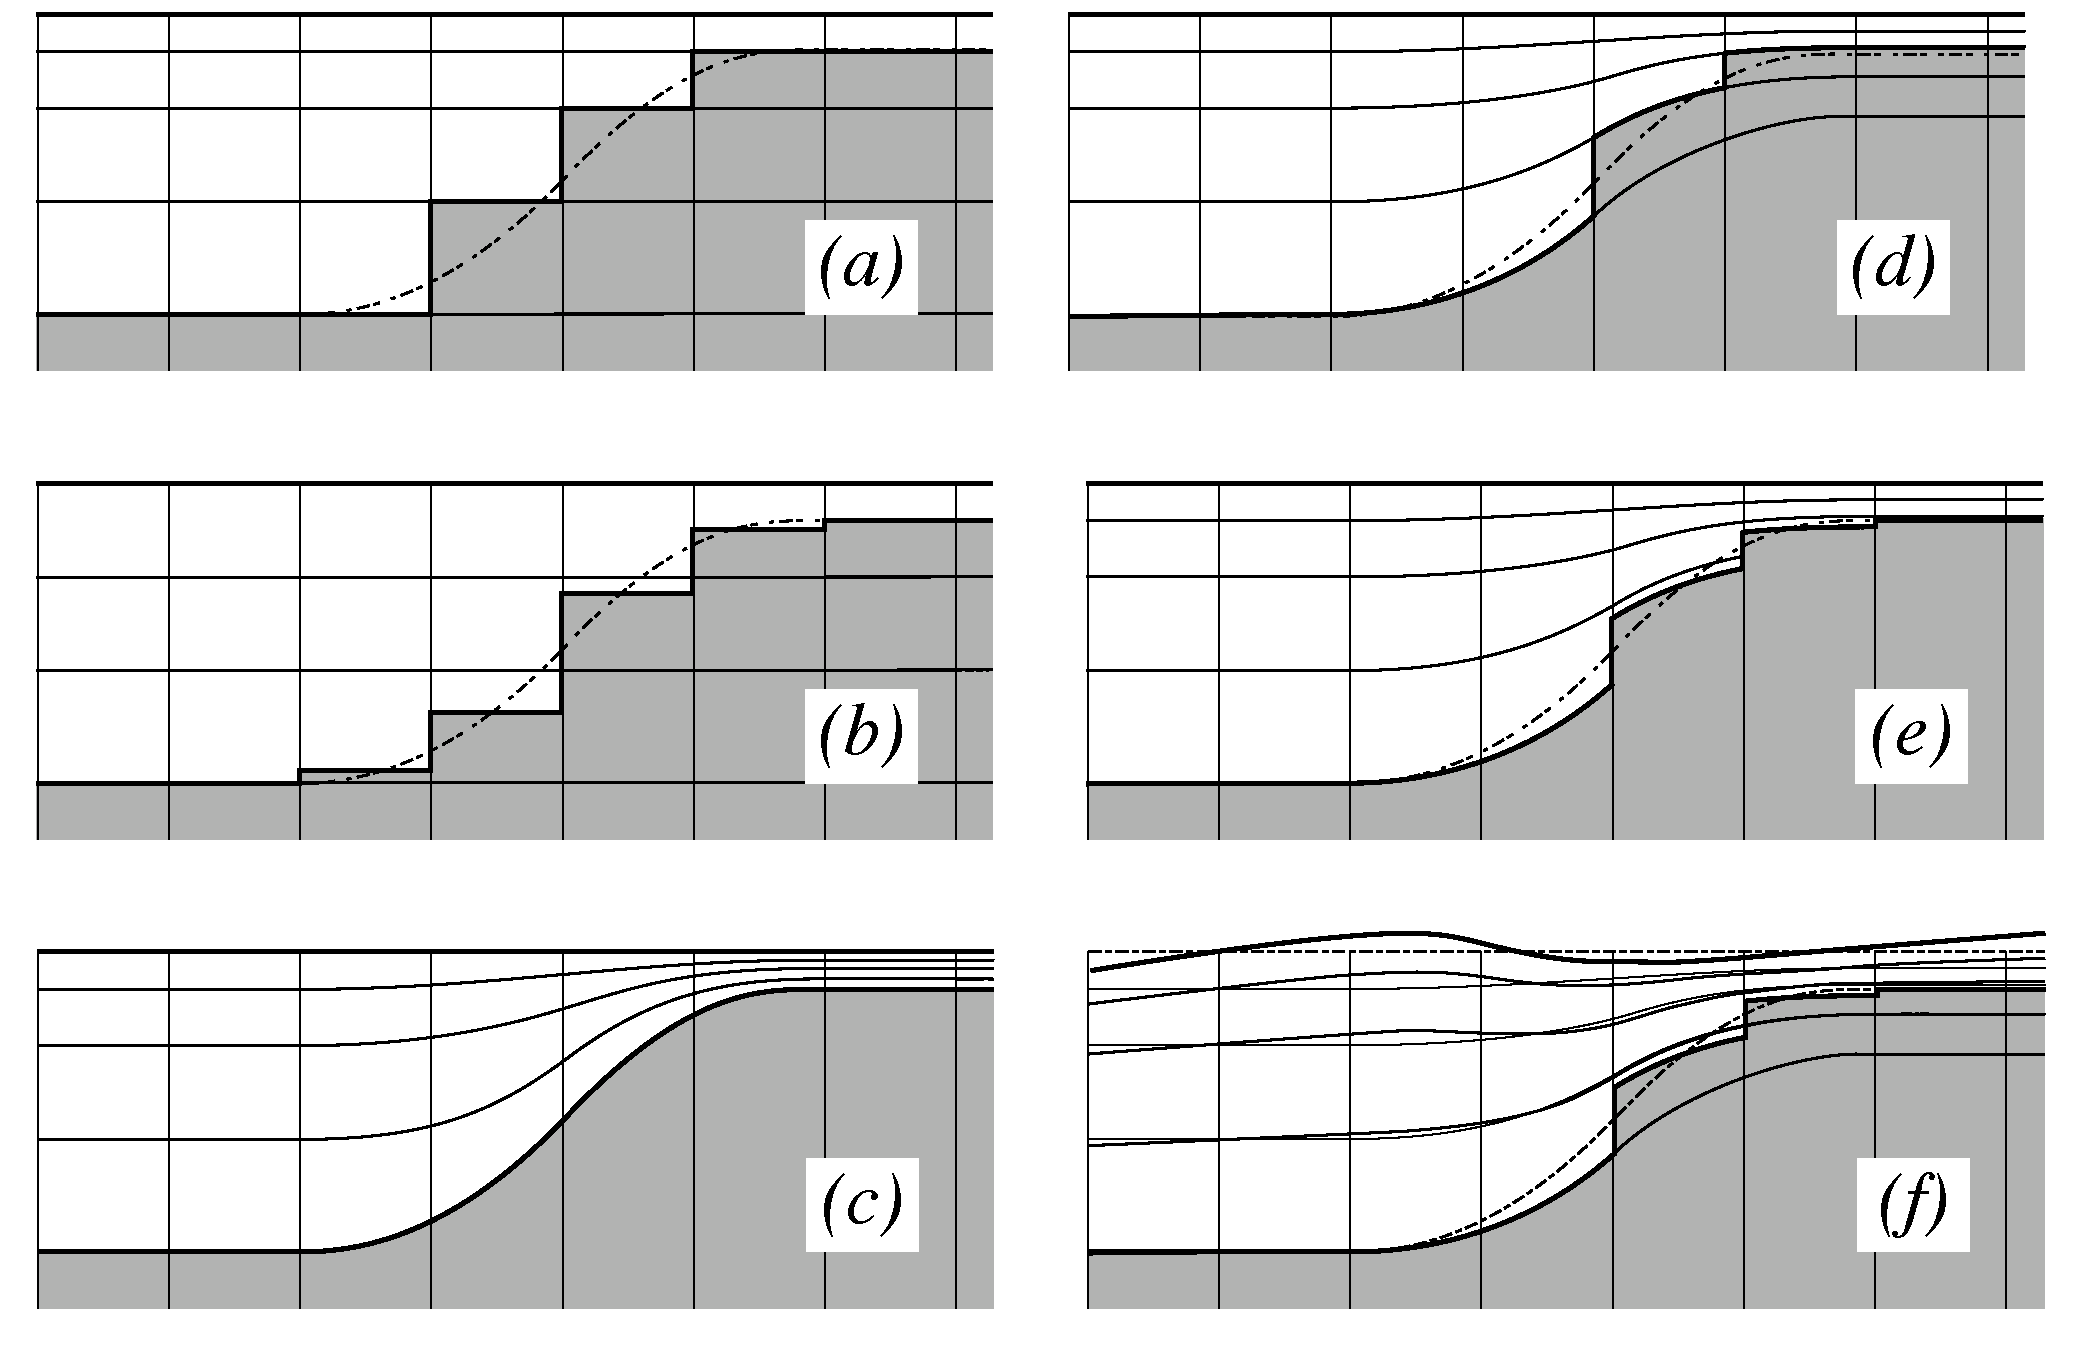
\includegraphics[width=1.0\textwidth]{./TexFiles/Figures/Fig_z_zps_s_sps.pdf}
\caption{  \label{Fig_z_zps_s_sps}   
The ocean bottom as seen by the model: 
(a) $z$-coordinate with full step, 
(b) $z$-coordinate with partial step, 
(c) $s$-coordinate: terrain following representation, 
(d) hybrid $s-z$ coordinate, 
(e) hybrid $s-z$ coordinate with partial step, and 
(f) same as (e) but with variable volume associated with the non-linear free surface. 
Note that the variable volume option (\key{vvl}) can be used with any of the 
5 coordinates (a) to (e).}
\end{center}   \end{figure}
%>>>>>>>>>>>>>>>>>>>>>>>>>>>>

The choice of a vertical coordinate, even if it is made through a namelist parameter, 
must be done once of all at the beginning of an experiment. It is not intended as an 
option which can be enabled or disabled in the middle of an experiment. Three main 
choices are offered (Fig.~\ref{Fig_z_zps_s_sps}a to c): $z$-coordinate with full step 
bathymetry (\np{ln\_zco}~=~true), $z$-coordinate with partial step bathymetry 
(\np{ln\_zps}~=~true), or generalized, $s$-coordinate (\np{ln\_sco}~=~true). 
Hybridation of the three main coordinates are available: $s-z$ or $s-zps$ coordinate 
(Fig.~\ref{Fig_z_zps_s_sps}d and \ref{Fig_z_zps_s_sps}e). When using the variable 
volume option \key{vvl} ($i.e.$ non-linear free surface), the coordinate follow the 
time-variation of the free surface so that the transformation is time dependent: 
$z(i,j,k,t)$ (Fig.~\ref{Fig_z_zps_s_sps}f). This option can be used with full step 
bathymetry or $s$-coordinate (hybrid and partial step coordinates have not 
yet been tested in NEMO v2.3). If using $z$-coordinate with partial step bathymetry
(\np{ln\_zps}~=~true), ocean cavity beneath ice shelves can be open (\np{ln\_isfcav}~=~true).

Contrary to the horizontal grid, the vertical grid is computed in the code and no 
provision is made for reading it from a file. The only input file is the bathymetry 
(in meters) (\ifile{bathy\_meter}) 
\footnote{N.B. in full step $z$-coordinate, a \ifile{bathy\_level} file can replace the 
\ifile{bathy\_meter} file, so that the computation of the number of wet ocean point 
in each water column is by-passed}. 
After reading the bathymetry, the algorithm for vertical grid definition differs 
between the different options:
\begin{description}
\item[\textit{zco}] set a reference coordinate transformation $z_0 (k)$, and set $z(i,j,k,t)=z_0 (k)$.
\item[\textit{zps}] set a reference coordinate transformation $z_0 (k)$, and 
calculate the thickness of the deepest level at each $(i,j)$ point using the 
bathymetry, to obtain the final three-dimensional depth and scale factor arrays.
\item[\textit{sco}] smooth the bathymetry to fulfil the hydrostatic consistency 
criteria and set the three-dimensional transformation.
\item[\textit{s-z} and \textit{s-zps}] smooth the bathymetry to fulfil the hydrostatic 
consistency criteria and set the three-dimensional transformation $z(i,j,k)$, and 
possibly introduce masking of extra land points to better fit the original bathymetry file
\end{description}
%%%
\gmcomment{   add the description of the smoothing:  envelop topography...}
%%%

The arrays describing the grid point depths and vertical scale factors 
are three dimensional arrays $(i,j,k)$ even in the case of $z$-coordinate with 
full step bottom topography. In non-linear free surface (\key{vvl}), their knowledge
is required at \textit{before}, \textit{now} and \textit{after} time step, while they 
do not vary in time in linear free surface case. 
To improve the code readability while providing this flexibility, the vertical coordinate 
and scale factors are defined as functions of 
$(i,j,k)$ with "fs" as prefix (examples: \textit{fse3t\_b, fse3t\_n, fse3t\_a,} 
for the  \textit{before}, \textit{now} and \textit{after} scale factors at $t$-point) 
that can be either three different arrays when \key{vvl} is defined, or a single fixed arrays. 
These functions are defined in the file \hf{domzgr\_substitute} of the DOM directory. 
They are used throughout the code, and replaced by the corresponding arrays at 
the time of pre-processing (CPP capability).

% -------------------------------------------------------------------------------------------------------------
%        Meter Bathymetry
% -------------------------------------------------------------------------------------------------------------
\subsection{Meter Bathymetry}
\label{DOM_bathy}

Three options are possible for defining the bathymetry, according to the 
namelist variable \np{nn\_bathy}: 
\begin{description}
\item[\np{nn\_bathy} = 0] a flat-bottom domain is defined. The total depth $z_w (jpk)$ 
is given by the coordinate transformation. The domain can either be a closed 
basin or a periodic channel depending on the parameter \np{jperio}. 
\item[\np{nn\_bathy} = -1] a domain with a bump of topography one third of the 
domain width at the central latitude. This is meant for the "EEL-R5" configuration, 
a periodic or open boundary channel with a seamount. 
\item[\np{nn\_bathy} = 1] read a bathymetry. The \ifile{bathy\_meter} file (Netcdf format) 
provides the ocean depth (positive, in meters) at each grid point of the model grid. 
The bathymetry is usually built by interpolating a standard bathymetry product 
($e.g.$ ETOPO2) onto the horizontal ocean mesh. Defining the bathymetry also 
defines the coastline: where the bathymetry is zero, no model levels are defined 
(all levels are masked).
\end{description}

When a global ocean is coupled to an atmospheric model it is better to represent 
all large water bodies (e.g, great lakes, Caspian sea...) even if the model 
resolution does not allow their communication with the rest of the ocean. 
This is unnecessary when the ocean is forced by fixed atmospheric conditions, 
so these seas can be removed from the ocean domain. The user has the option 
to set the bathymetry in closed seas to zero (see \S\ref{MISC_closea}), but the 
code has to be adapted to the user's configuration. 

% -------------------------------------------------------------------------------------------------------------
%        z-coordinate  and reference coordinate transformation
% -------------------------------------------------------------------------------------------------------------
\subsection[$z$-coordinate (\np{ln\_zco}]
	  	  {$z$-coordinate (\np{ln\_zco}=true) and reference coordinate}
\label{DOM_zco}

%>>>>>>>>>>>>>>>>>>>>>>>>>>>>
\begin{figure}[!tb]    \begin{center}
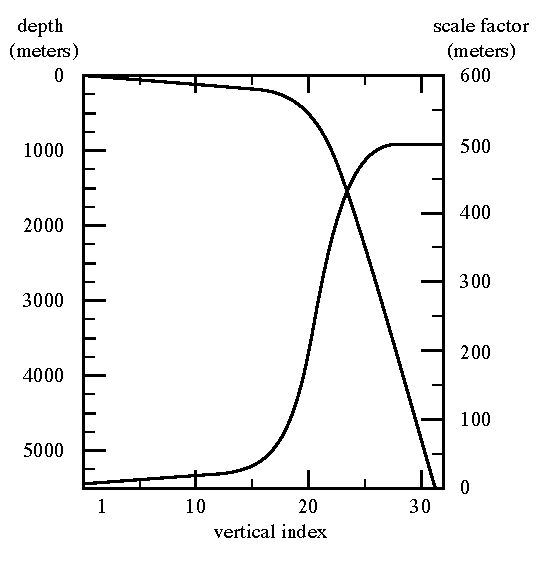
\includegraphics[width=0.90\textwidth]{./TexFiles/Figures/Fig_zgr.pdf}
\caption{ \label{Fig_zgr}    
Default vertical mesh for ORCA2: 30 ocean levels (L30). Vertical level functions for 
(a) T-point depth and (b) the associated scale factor as computed 
from \eqref{DOM_zgr_ana} using \eqref{DOM_zgr_coef} in $z$-coordinate.}
\end{center}   \end{figure}
%>>>>>>>>>>>>>>>>>>>>>>>>>>>>

The reference coordinate transformation $z_0 (k)$ defines the arrays $gdept_0$ 
and $gdepw_0$ for $t$- and $w$-points, respectively. As indicated on 
Fig.\ref{Fig_index_vert} \jp{jpk} is the number of $w$-levels. $gdepw_0(1)$ is the 
ocean surface. There are at most \jp{jpk}-1 $t$-points inside the ocean, the 
additional $t$-point at $jk=jpk$ is below the sea floor and is not used. 
The vertical location of $w$- and $t$-levels is defined from the analytic expression 
of the depth $z_0(k)$ whose analytical derivative with respect to $k$ provides the 
vertical scale factors. The user must provide the analytical expression of both 
$z_0$ and its first derivative with respect to $k$. This is done in routine \mdl{domzgr} 
through statement functions, using parameters provided in the \ngn{namcfg} namelist. 

It is possible to define a simple regular vertical grid by giving zero stretching (\np{ppacr=0}). 
In that case, the parameters \jp{jpk} (number of $w$-levels) and \np{pphmax} 
(total ocean depth in meters) fully define the grid. 

For climate-related studies it is often desirable to concentrate the vertical resolution 
near the ocean surface. The following function is proposed as a standard for a 
$z$-coordinate (with either full or partial steps): 
\begin{equation} \label{DOM_zgr_ana}
\begin{split}
 z_0 (k) 	&= h_{sur} -h_0 \;k-\;h_1 \;\log \left[ {\,\cosh \left( {{(k-h_{th} )} / {h_{cr} }} \right)\,} \right] \\ 
 e_3^0 (k) 	&= \left| -h_0 -h_1 \;\tanh \left( {{(k-h_{th} )} / {h_{cr} }} \right) \right| 
\end{split}
\end{equation}
where $k=1$ to \jp{jpk} for $w$-levels and $k=1$ to $k=1$ for $T-$levels. Such an 
expression allows us to define a nearly uniform vertical location of levels at the 
ocean top and bottom with a smooth hyperbolic tangent transition in between 
(Fig.~\ref{Fig_zgr}).

The most used vertical grid for ORCA2 has $10~m$ ($500~m)$ resolution in the 
surface (bottom) layers and a depth which varies from 0 at the sea surface to a 
minimum of $-5000~m$. This leads to the following conditions:
\begin{equation} \label{DOM_zgr_coef}
\begin{split}
 e_3 (1+1/2)		&=10. \\ 
 e_3 (jpk-1/2)	&=500. \\ 
 z(1)			&=0. \\ 
 z(jpk)			&=-5000. \\ 
\end{split}
\end{equation}

With the choice of the stretching $h_{cr} =3$ and the number of levels 
\jp{jpk}=$31$, the four coefficients $h_{sur}$, $h_{0}$, $h_{1}$, and $h_{th}$ in 
\eqref{DOM_zgr_ana} have been determined such that \eqref{DOM_zgr_coef} is 
satisfied, through an optimisation procedure using a bisection method. For the first 
standard ORCA2 vertical grid this led to the following values: $h_{sur} =4762.96$, 
$h_0 =255.58, h_1 =245.5813$, and $h_{th} =21.43336$. The resulting depths and 
scale factors as a function of the model levels are shown in Fig.~\ref{Fig_zgr} and 
given in Table \ref{Tab_orca_zgr}. Those values correspond to the parameters 
\np{ppsur}, \np{ppa0}, \np{ppa1}, \np{ppkth} in \ngn{namcfg} namelist. 

Rather than entering parameters $h_{sur}$, $h_{0}$, and $h_{1}$ directly, it is 
possible to recalculate them. In that case the user sets 
\np{ppsur}=\np{ppa0}=\np{ppa1}=999999., in \ngn{namcfg} namelist, 
and specifies instead the four following parameters:
\begin{itemize}
\item 	\np{ppacr}=$h_{cr} $: stretching factor (nondimensional). The larger 
\np{ppacr}, the smaller the stretching. Values from $3$ to $10$ are usual.
\item 	\np{ppkth}=$h_{th} $: is approximately the model level at which maximum 
stretching occurs (nondimensional, usually of order 1/2 or 2/3 of \jp{jpk})
\item 	\np{ppdzmin}: minimum thickness for the top layer (in meters)
\item 	\np{pphmax}: total depth of the ocean (meters).
\end{itemize}
As an example, for the $45$ layers used in the DRAKKAR configuration those 
parameters are: \jp{jpk}=46, \np{ppacr}=9, \np{ppkth}=23.563, \np{ppdzmin}=6m, 
\np{pphmax}=5750m.

%>>>>>>>>>>>>>>>>>>>>>>>>>>>>
\begin{table}     \begin{center} \begin{tabular}{c||r|r|r|r}
\hline
\textbf{LEVEL}& \textbf{gdept}& \textbf{gdepw}& \textbf{e3t }& \textbf{e3w  } \\ \hline
1	&	\textbf{  5.00}	&       0.00 &	\textbf{ 10.00} &	 10.00 \\	\hline
2	&	\textbf{15.00}	& 	  10.00 &	\textbf{ 10.00} &	 10.00 \\	\hline
3	&	\textbf{25.00}	&	  20.00 &	\textbf{ 10.00} & 	 10.00 \\	\hline
4	&	\textbf{35.01}	&	  30.00 & 	\textbf{ 10.01} & 	 10.00 \\	\hline
5	&	\textbf{45.01}	&	  40.01 &	\textbf{ 10.01} &	 10.01 \\	\hline
6	&	\textbf{55.03}	&	  50.02 &	\textbf{ 10.02} & 	 10.02 \\	\hline
7	&	\textbf{65.06}	&	  60.04 &	\textbf{ 10.04} &	 10.03 \\	\hline
8	&	\textbf{75.13}	&	  70.09 &	\textbf{ 10.09} &	 10.06 \\	\hline
9	&	\textbf{85.25}	&	  80.18 &	\textbf{ 10.17} &	 10.12 \\	\hline
10	& 	\textbf{95.49}	& 	  90.35 &	\textbf{ 10.33} &	 10.24 \\	\hline
11	& 	\textbf{105.97}	& 	 100.69 &	\textbf{ 10.65} &	 10.47 \\	\hline
12	& 	\textbf{116.90}	& 	 111.36 &	\textbf{ 11.27} &	 10.91 \\	\hline
13	& 	\textbf{128.70}	& 	 122.65 &	\textbf{ 12.47} &	 11.77 \\	\hline
14	& 	\textbf{142.20}	& 	 135.16 &	\textbf{ 14.78} &	 13.43 \\	\hline
15	& 	\textbf{158.96}	& 	 150.03 &	\textbf{ 19.23} &	 16.65 \\	\hline
16	& 	\textbf{181.96}	& 	 169.42 &	\textbf{ 27.66} &	 22.78 \\	\hline
17	& 	\textbf{216.65}	& 	 197.37 & 	\textbf{ 43.26} &	 34.30 \\ \hline
18	& 	\textbf{272.48}	& 	 241.13 & 	\textbf{ 70.88} &	 55.21 \\ \hline
19	& 	\textbf{364.30}	& 	 312.74 & 	\textbf{116.11} &	 90.99 \\ \hline
20	& 	\textbf{511.53}	& 	 429.72 & 	\textbf{181.55} & 	146.43 \\ \hline
21	& 	\textbf{732.20}	& 	 611.89 & 	\textbf{261.03} & 	220.35 \\ \hline
22	& 	\textbf{1033.22}&	 872.87 & 	\textbf{339.39} & 	301.42 \\ \hline
23	& 	\textbf{1405.70}&	1211.59 & \textbf{402.26} & 	373.31 \\ \hline
24	& 	\textbf{1830.89}&	1612.98 & \textbf{444.87} & 	426.00 \\ \hline
25	& 	\textbf{2289.77}&	2057.13 & \textbf{470.55} & 	459.47 \\ \hline
26	& 	\textbf{2768.24}&	2527.22 & \textbf{484.95} & 	478.83 \\ \hline
27	& 	\textbf{3257.48}&	3011.90 & \textbf{492.70} & 	489.44 \\ \hline
28	& 	\textbf{3752.44}&	3504.46 & \textbf{496.78} & 	495.07 \\ \hline
29	& 	\textbf{4250.40}&	4001.16 & \textbf{498.90} & 	498.02 \\ \hline
30	& 	\textbf{4749.91}&	4500.02 & \textbf{500.00} &	499.54 \\ \hline
31	& 	\textbf{5250.23}&	5000.00 &	\textbf{500.56} &	500.33 \\ \hline
\end{tabular} \end{center} 
\caption{ \label{Tab_orca_zgr}   
Default vertical mesh in $z$-coordinate for 30 layers ORCA2 configuration as computed 
from \eqref{DOM_zgr_ana} using the coefficients given in \eqref{DOM_zgr_coef}}
\end{table}
%>>>>>>>>>>>>>>>>>>>>>>>>>>>>

% -------------------------------------------------------------------------------------------------------------
%        z-coordinate with partial step
% -------------------------------------------------------------------------------------------------------------
\subsection   [$z$-coordinate with partial step (\np{ln\_zps})]
			{$z$-coordinate with partial step (\np{ln\_zps}=.true.)}
\label{DOM_zps}
%--------------------------------------------namdom-------------------------------------------------------
\namdisplay{namdom} 
%--------------------------------------------------------------------------------------------------------------

In $z$-coordinate partial step, the depths of the model levels are defined by the 
reference analytical function $z_0 (k)$ as described in the previous 
section, \emph{except} in the bottom layer. The thickness of the bottom layer is 
allowed to vary as a function of geographical location $(\lambda,\varphi)$ to allow a 
better representation of the bathymetry, especially in the case of small 
slopes (where the bathymetry varies by less than one level thickness from 
one grid point to the next). The reference layer thicknesses $e_{3t}^0$ have been 
defined in the absence of bathymetry. With partial steps, layers from 1 to 
\jp{jpk}-2 can have a thickness smaller than $e_{3t}(jk)$. The model deepest layer (\jp{jpk}-1) 
is allowed to have either a smaller or larger thickness than $e_{3t}(jpk)$: the 
maximum thickness allowed is $2*e_{3t}(jpk-1)$. This has to be kept in mind when 
specifying values in \ngn{namdom} namelist, as the maximum depth \np{pphmax} 
in partial steps: for example, with 
\np{pphmax}$=5750~m$ for the DRAKKAR 45 layer grid, the maximum ocean depth 
allowed is actually $6000~m$ (the default thickness $e_{3t}(jpk-1)$ being $250~m$). 
Two variables in the namdom namelist are used to define the partial step 
vertical grid. The mimimum water thickness (in meters) allowed for a cell 
partially filled with bathymetry at level jk is the minimum of \np{rn\_e3zps\_min} 
(thickness in meters, usually $20~m$) or $e_{3t}(jk)*\np{rn\_e3zps\_rat}$ (a fraction, 
usually 10\%, of the default thickness $e_{3t}(jk)$).

 \colorbox{yellow}{Add a figure here of pstep especially at last ocean level }

% -------------------------------------------------------------------------------------------------------------
%        s-coordinate
% -------------------------------------------------------------------------------------------------------------
\subsection   [$s$-coordinate (\np{ln\_sco})]
		     {$s$-coordinate (\np{ln\_sco}=true)}
\label{DOM_sco}
%------------------------------------------nam_zgr_sco---------------------------------------------------
\namdisplay{namzgr_sco} 
%--------------------------------------------------------------------------------------------------------------
Options are defined in \ngn{namzgr\_sco}.
In $s$-coordinate (\np{ln\_sco}~=~true), the depth and thickness of the model 
levels are defined from the product of a depth field and either a stretching 
function or its derivative, respectively:

\begin{equation} \label{DOM_sco_ana}
\begin{split}
 z(k) 		&= h(i,j) \; z_0(k)	\\
 e_3(k)	&= h(i,j) \; z_0'(k)
\end{split}
\end{equation}

where $h$ is the depth of the last $w$-level ($z_0(k)$) defined at the $t$-point 
location in the horizontal and $z_0(k)$ is a function which varies from $0$ at the sea 
surface to $1$ at the ocean bottom. The depth field $h$ is not necessary the ocean 
depth, since a mixed step-like and bottom-following representation of the 
topography can be used (Fig.~\ref{Fig_z_zps_s_sps}d-e) or an envelop bathymetry can be defined (Fig.~\ref{Fig_z_zps_s_sps}f).
The namelist parameter \np{rn\_rmax} determines the slope at which the terrain-following coordinate intersects the sea bed and becomes a pseudo z-coordinate. The coordinate can also be hybridised by specifying \np{rn\_sbot\_min} and \np{rn\_sbot\_max} as the minimum and maximum depths at which the terrain-following vertical coordinate is calculated.

Options for stretching the coordinate are provided as examples, but care must be taken to ensure that the vertical stretch used is appropriate for the application.

The original default NEMO s-coordinate stretching is available if neither of the other options are specified as true (\np{ln\_sco\_SH94}~=~false and \np{ln\_sco\_SF12}~=~false.) This uses a depth independent $\tanh$ function for the stretching \citep{Madec_al_JPO96}:

\begin{equation}
  z = s_{min}+C\left(s\right)\left(H-s_{min}\right)
  \label{eq:SH94_1}
\end{equation}

where $s_{min}$ is the depth at which the s-coordinate stretching starts and allows a z-coordinate to placed on top of the stretched coordinate, and z is the depth (negative down from the asea surface).

\begin{equation}
  s = -\frac{k}{n-1} \quad \text{ and } \quad 0 \leq k \leq n-1
  \label{eq:s}
\end{equation}

\begin{equation} \label{DOM_sco_function}
\begin{split}
C(s)	&=  \frac{ \left[	  \tanh{ \left( \theta \, (s+b) \right)} 
	  	 			- \tanh{ \left(  \theta \, b      \right)}  \right]}
		      {2\;\sinh \left( \theta \right)}
\end{split}
\end{equation}

A stretching function, modified from the commonly used \citet{Song_Haidvogel_JCP94} stretching (\np{ln\_sco\_SH94}~=~true), is also available and is more commonly used for shelf seas modelling:

\begin{equation}
  C\left(s\right) =   \left(1 - b \right)\frac{ \sinh\left( \theta s\right)}{\sinh\left(\theta\right)} +      \\
  b\frac{ \tanh \left[ \theta \left(s + \frac{1}{2} \right)\right] - \tanh\left(\frac{\theta}{2}\right)}{ 2\tanh\left (\frac{\theta}{2}\right)}
  \label{eq:SH94_2}
\end{equation}

%>>>>>>>>>>>>>>>>>>>>>>>>>>>>
\begin{figure}[!ht]    \begin{center}
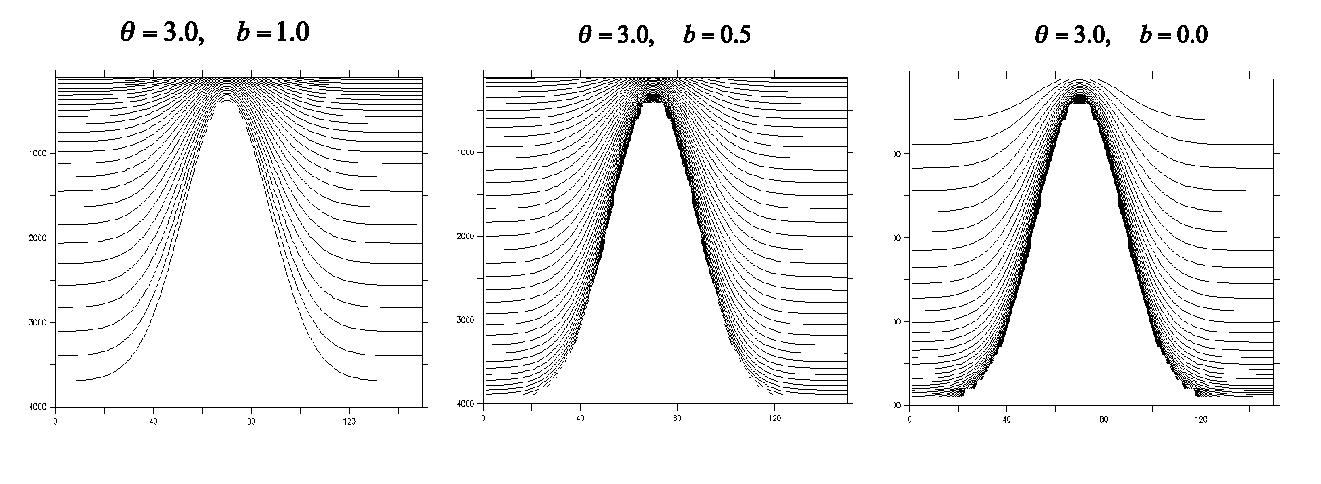
\includegraphics[width=1.0\textwidth]{./TexFiles/Figures/Fig_sco_function.pdf}
\caption{  \label{Fig_sco_function}   
Examples of the stretching function applied to a seamount; from left to right: 
surface, surface and bottom, and bottom intensified resolutions}
\end{center}   \end{figure}
%>>>>>>>>>>>>>>>>>>>>>>>>>>>>

where $H_c$ is the critical depth (\np{rn\_hc}) at which the coordinate transitions from pure $\sigma$ to the stretched coordinate,  and $\theta$ (\np{rn\_theta}) and $b$ (\np{rn\_bb}) are the surface and 
bottom control parameters such that $0\leqslant \theta \leqslant 20$, and 
$0\leqslant b\leqslant 1$. $b$ has been designed to allow surface and/or bottom 
increase of the vertical resolution (Fig.~\ref{Fig_sco_function}).

Another example has been provided at version 3.5 (\np{ln\_sco\_SF12}) that allows a fixed surface resolution in an analytical terrain-following stretching \citet{Siddorn_Furner_OM12}. In this case the a stretching function $\gamma$ is defined such that:

\begin{equation}
z = -\gamma h \quad \text{ with } \quad 0 \leq \gamma \leq 1
\label{eq:z}
\end{equation}

The function is defined with respect to $\sigma$, the unstretched terrain-following coordinate:

\begin{equation} \label{DOM_gamma_deriv}
\gamma= A\left(\sigma-\frac{1}{2}\left(\sigma^{2}+f\left(\sigma\right)\right)\right)+B\left(\sigma^{3}-f\left(\sigma\right)\right)+f\left(\sigma\right)
\end{equation}

Where:
\begin{equation} \label{DOM_gamma}
f\left(\sigma\right)=\left(\alpha+2\right)\sigma^{\alpha+1}-\left(\alpha+1\right)\sigma^{\alpha+2} \quad \text{ and } \quad \sigma = \frac{k}{n-1} 
\end{equation}

This gives an analytical stretching of $\sigma$ that is solvable in $A$ and $B$ as a function of the user prescribed stretching parameter $\alpha$ (\np{rn\_alpha}) that stretches towards the surface ($\alpha > 1.0$) or the bottom ($\alpha < 1.0$) and user prescribed surface (\np{rn\_zs}) and bottom depths. The bottom cell depth in this example is given as a function of water depth:

\begin{equation} \label{DOM_zb}
Z_b= h a + b
\end{equation}

where the namelist parameters \np{rn\_zb\_a} and \np{rn\_zb\_b} are $a$ and $b$ respectively.

%>>>>>>>>>>>>>>>>>>>>>>>>>>>>
\begin{figure}[!ht]
   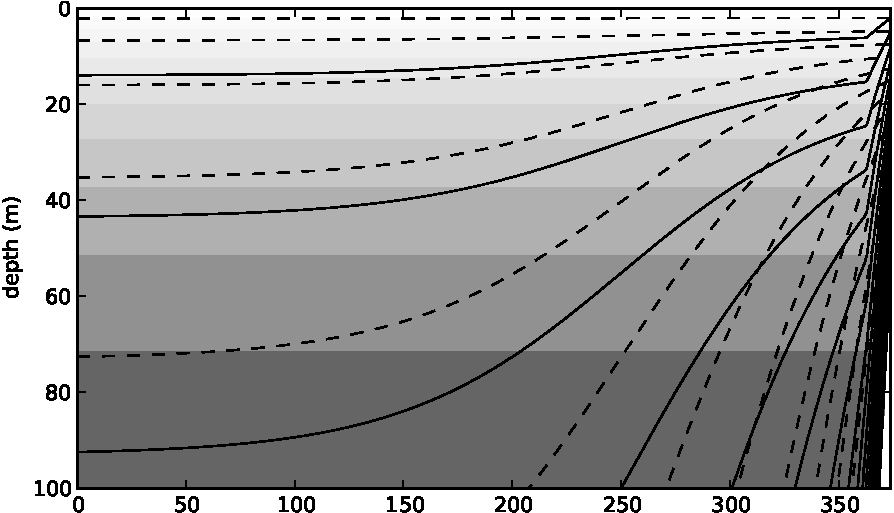
\includegraphics[width=1.0\textwidth]{./TexFiles/Figures/FIG_DOM_compare_coordinates_surface.pdf}
        \caption{A comparison of the \citet{Song_Haidvogel_JCP94} $S$-coordinate (solid lines), a 50 level $Z$-coordinate (contoured surfaces) and the \citet{Siddorn_Furner_OM12} $S$-coordinate (dashed lines) in the surface 100m for a idealised bathymetry that goes from 50m to 5500m depth. For clarity every third coordinate surface is shown.}
    \label{fig_compare_coordinates_surface}
\end{figure}
%>>>>>>>>>>>>>>>>>>>>>>>>>>>>

This gives a smooth analytical stretching in computational space that is constrained to given specified surface and bottom grid cell thicknesses in real space. This is not to be confused with the hybrid schemes that superimpose geopotential coordinates on terrain following coordinates thus creating a non-analytical vertical coordinate that therefore may suffer from large gradients in the vertical resolutions. This stretching is less straightforward to implement than the \citet{Song_Haidvogel_JCP94} stretching, but has the advantage of resolving diurnal processes in deep water and has generally flatter slopes.

As with the \citet{Song_Haidvogel_JCP94} stretching the stretch is only applied at depths greater than the critical depth $h_c$. In this example two options are available in depths shallower than $h_c$, with pure sigma being applied if the \np{ln\_sigcrit} is true and pure z-coordinates if it is false (the z-coordinate being equal to the depths of the stretched coordinate at $h_c$.

Minimising the horizontal slope of the vertical coordinate is important in terrain-following systems as large slopes lead to hydrostatic consistency. A hydrostatic consistency parameter diagnostic following \citet{Haney1991} has been implemented, and is output as part of the model mesh file at the start of the run.

% -------------------------------------------------------------------------------------------------------------
%        z*- or s*-coordinate
% -------------------------------------------------------------------------------------------------------------
\subsection{$z^*$- or $s^*$-coordinate (add \key{vvl}) }
\label{DOM_zgr_vvl}

This option is described in the Report by Levier \textit{et al.} (2007), available on 
the \NEMO web site. 

%gm% key advantage: minimise the diffusion/dispertion associated with advection in response to high frequency surface disturbances

% -------------------------------------------------------------------------------------------------------------
%        level bathymetry and mask 
% -------------------------------------------------------------------------------------------------------------
\subsection{level bathymetry and mask}
\label{DOM_msk}

Whatever the vertical coordinate used, the model offers the possibility of 
representing the bottom topography with steps that follow the face of the 
model cells (step like topography) \citep{Madec_al_JPO96}. The distribution of 
the steps in the horizontal is defined in a 2D integer array, mbathy, which 
gives the number of ocean levels ($i.e.$ those that are not masked) at each 
$t$-point. mbathy is computed from the meter bathymetry using the definiton of 
gdept as the number of $t$-points which gdept $\leq$ bathy. 

Modifications of the model bathymetry are performed in the \textit{bat\_ctl} 
routine (see \mdl{domzgr} module) after mbathy is computed. Isolated grid points 
that do not communicate with another ocean point at the same level are eliminated.

From the \textit{mbathy} array, the mask fields are defined as follows:
\begin{align*}
tmask(i,j,k) &= \begin{cases}   \; 1&   \text{ if $k\leq mbathy(i,j)$  }    \\
                                                \; 0&   \text{ if $k\leq mbathy(i,j)$  }    \end{cases}     \\
umask(i,j,k) &=         \; tmask(i,j,k) \ * \ tmask(i+1,j,k)	\\
vmask(i,j,k) &=         \; tmask(i,j,k) \ * \ tmask(i,j+1,k)	\\
fmask(i,j,k) &=         \; tmask(i,j,k) \ * \ tmask(i+1,j,k)	\\
                   & \ \ \, * tmask(i,j,k) \ * \ tmask(i+1,j,k)
\end{align*}

Note that \textit{wmask} is not defined as it is exactly equal to \textit{tmask} with 
the numerical indexing used (\S~\ref{DOM_Num_Index}). Moreover, the 
specification of closed lateral boundaries requires that at least the first and last 
rows and columns of the \textit{mbathy} array are set to zero. In the particular 
case of an east-west cyclical boundary condition, \textit{mbathy} has its last 
column equal to the second one and its first column equal to the last but one 
(and so too the mask arrays) (see \S~\ref{LBC_jperio}).

%%%
\gmcomment{   \colorbox{yellow}{Add one word on tricky trick !} mbathy in further modified in zdfbfr{\ldots}.  }
%%%

% ================================================================
% Domain: Initial State (dtatsd & istate)
% ================================================================
\section  [Domain: Initial State (\textit{istate and dtatsd})]
		{Domain: Initial State \small{(\mdl{istate} and \mdl{dtatsd} modules)} }
\label{DTA_tsd}
%-----------------------------------------namtsd-------------------------------------------
\namdisplay{namtsd} 
%------------------------------------------------------------------------------------------

Options are defined in \ngn{namtsd}.
By default, the ocean start from rest (the velocity field is set to zero) and the initialization of 
temperature and salinity fields is controlled through the \np{ln\_tsd\_ini} namelist parameter.
\begin{description}
\item[ln\_tsd\_init = .true.]  use a T and S input files that can be given on the model grid itself or 
on their native input data grid. In the latter case, the data will be interpolated on-the-fly both in the 
horizontal and the vertical to the model grid (see \S~\ref{SBC_iof}). The information relative to the 
input files are given in the \np{sn\_tem} and \np{sn\_sal} structures. 
The computation is done in the \mdl{dtatsd} module.
\item[ln\_tsd\_init = .false.] use constant salinity value of 35.5 psu and an analytical profile of temperature
(typical of the tropical ocean), see \rou{istate\_t\_s} subroutine called from \mdl{istate} module.
\end{description}
			% Space discretisation

% ================================================================
% Chapter 1 ——— Ocean Tracers (TRA)
% ================================================================
\chapter{Ocean Tracers (TRA)}
\label{TRA}
\minitoc

% missing/update 
% traqsr: need to coordinate with SBC module

%STEVEN :  is the use of the word "positive" to describe a scheme enough, or should it be "positive definite"? I added a comment to this effect on some instances of this below

%\newpage
\vspace{2.cm}
%$\ $\newline    % force a new ligne

Using the representation described in Chap.~\ref{DOM}, several semi-discrete 
space forms of the tracer equations are available depending on the vertical 
coordinate used and on the physics used. In all the equations presented 
here, the masking has been omitted for simplicity. One must be aware that 
all the quantities are masked fields and that each time a mean or difference 
operator is used, the resulting field is multiplied by a mask.

The two active tracers are potential temperature and salinity. Their prognostic 
equations can be summarized as follows:
\begin{equation*}
\text{NXT} = \text{ADV}+\text{LDF}+\text{ZDF}+\text{SBC}
                   \ (+\text{QSR})\ (+\text{BBC})\ (+\text{BBL})\ (+\text{DMP})
\end{equation*}

NXT stands for next, referring to the time-stepping. From left to right, the terms 
on the rhs of the tracer equations are the advection (ADV), the lateral diffusion 
(LDF), the vertical diffusion (ZDF), the contributions from the external forcings 
(SBC: Surface Boundary Condition, QSR: penetrative Solar Radiation, and BBC: 
Bottom Boundary Condition), the contribution from the bottom boundary Layer 
(BBL) parametrisation, and an internal damping (DMP) term. The terms QSR, 
BBC, BBL and DMP are optional. The external forcings and parameterisations 
require complex inputs and complex calculations (e.g. bulk formulae, estimation 
of mixing coefficients) that are carried out in the SBC, LDF and ZDF modules and 
described in chapters \S\ref{SBC}, \S\ref{LDF} and  \S\ref{ZDF}, respectively. 
Note that \mdl{tranpc}, the non-penetrative convection module,  although 
(temporarily) located in the NEMO/OPA/TRA directory, is described with the 
model vertical physics (ZDF).
%%%
\gmcomment{change the position of eosbn2 in the reference code}
%%%

In the present chapter we also describe the diagnostic equations used to compute 
the sea-water properties (density, Brunt-Vais\"{a}l\"{a} frequency, specific heat and 
freezing point with associated modules \mdl{eosbn2} and \mdl{phycst}).

The different options available to the user are managed by namelist logicals or 
CPP keys. For each equation term \textit{ttt}, the namelist logicals are \textit{ln\_trattt\_xxx}, 
where \textit{xxx} is a 3 or 4 letter acronym corresponding to each optional scheme. 
The CPP key (when it exists) is \textbf{key\_trattt}. The equivalent code can be 
found in the \textit{trattt} or \textit{trattt\_xxx} module, in the NEMO/OPA/TRA directory.

The user has the option of extracting each tendency term on the rhs of the tracer 
equation for output (\key{trdtra} is defined), as described in Chap.~\ref{MISC}.

$\ $\newline    % force a new ligne
% ================================================================
% Tracer Advection
% ================================================================
\section  [Tracer Advection (\textit{traadv})]
		{Tracer Advection (\mdl{traadv})}
\label{TRA_adv}
%------------------------------------------namtra_adv-----------------------------------------------------
\namdisplay{namtra_adv}
%-------------------------------------------------------------------------------------------------------------

The advection tendency of a tracer in flux form is the divergence of the advective 
fluxes. Its discrete expression is given by :
\begin{equation} \label{Eq_tra_adv}
ADV_\tau =-\frac{1}{b_t} \left( 
\;\delta _i \left[ e_{2u}\,e_{3u} \;  u\; \tau _u  \right]
+\delta _j \left[ e_{1v}\,e_{3v}  \;  v\; \tau _v  \right] \; \right)
-\frac{1}{e_{3t}} \;\delta _k \left[ w\; \tau _w \right]
\end{equation}
where $\tau$ is either T or S, and $b_t= e_{1t}\,e_{2t}\,e_{3t}$ is the volume of $T$-cells. 
The flux form in \eqref{Eq_tra_adv} 
implicitly requires the use of the continuity equation. Indeed, it is obtained
by using the following equality : $\nabla \cdot \left( \vect{U}\,T \right)=\vect{U} \cdot \nabla T$ 
which results from the use of the continuity equation, $\nabla \cdot \vect{U}=0$ or 
$ \partial _t e_3 + e_3\;\nabla \cdot \vect{U}=0$ in constant volume or variable volume case, respectively. 
Therefore it is of paramount importance to design the discrete analogue of the 
advection tendency so that it is consistent with the continuity equation in order to 
enforce the conservation properties of the continuous equations. In other words, 
by replacing $\tau$ by the number 1 in (\ref{Eq_tra_adv}) we recover the discrete form of 
the continuity equation which is used to calculate the vertical velocity.
%>>>>>>>>>>>>>>>>>>>>>>>>>>>>
\begin{figure}[!t] 	 \begin{center}
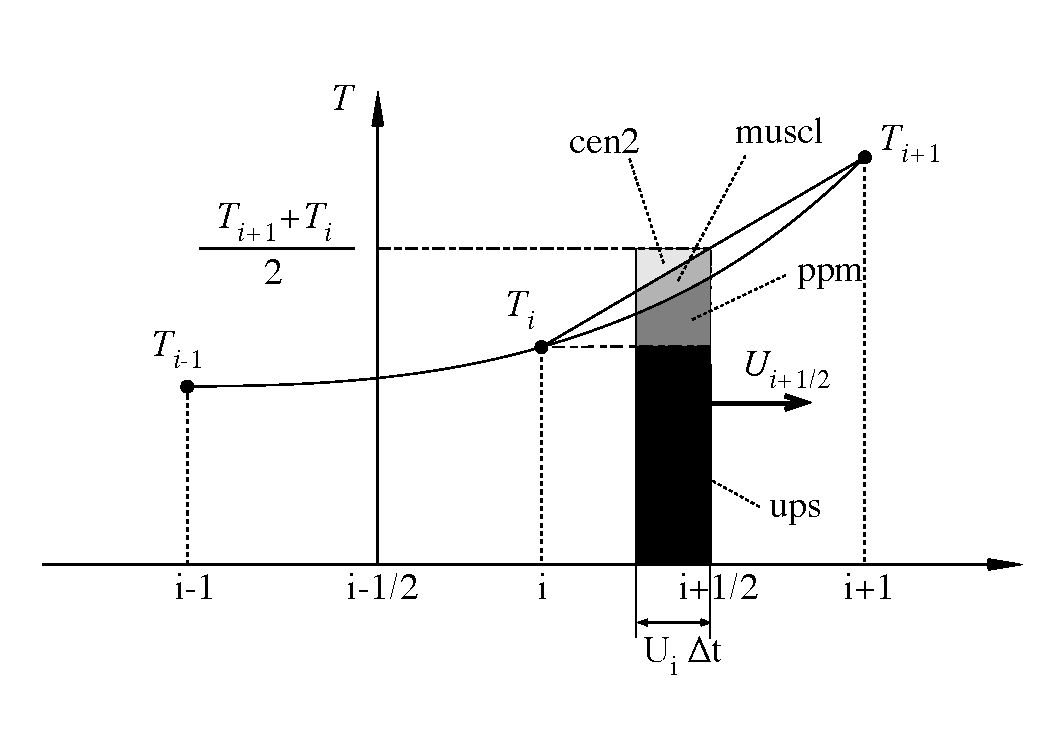
\includegraphics[width=0.9\textwidth]{./TexFiles/Figures/Fig_adv_scheme.pdf}
\caption{	\label{Fig_adv_scheme} 
Schematic representation of some ways used to evaluate the tracer value 
at $u$-point and the amount of tracer exchanged between two neighbouring grid 
points. Upsteam biased scheme (ups): the upstream value is used and the black 
area is exchanged. Piecewise parabolic method (ppm): a parabolic interpolation 
is used and the black and dark grey areas are exchanged. Monotonic upstream 
scheme for conservative laws (muscl):  a parabolic interpolation is used and black, 
dark grey and grey areas are exchanged. Second order scheme (cen2): the mean 
value is used and black, dark grey, grey and light grey areas are exchanged. Note 
that this illustration does not include the flux limiter used in ppm and muscl schemes.}
\end{center}   \end{figure}
%>>>>>>>>>>>>>>>>>>>>>>>>>>>>

The key difference between the advection schemes available in \NEMO is the choice 
made in space and time interpolation to define the value of the tracer at the 
velocity points (Fig.~\ref{Fig_adv_scheme}). 

Along solid lateral and bottom boundaries a zero tracer flux is automatically 
specified, since the normal velocity is zero there. At the sea surface the 
boundary condition depends on the type of sea surface chosen: 
\begin{description}
\item [linear free surface:] the first level thickness is constant in time: 
the vertical boundary condition is applied at the fixed surface $z=0$ 
rather than on the moving surface $z=\eta$. There is a non-zero advective 
flux which is set for all advection schemes as 
$\left. {\tau _w } \right|_{k=1/2} =T_{k=1} $, $i.e.$ 
the product of surface velocity (at $z=0$) by the first level tracer value.
\item [non-linear free surface:] (\key{vvl} is defined) 
convergence/divergence in the first ocean level moves the free surface 
up/down. There is no tracer advection through it so that the advective 
fluxes through the surface are also zero 
\end{description}
In all cases, this boundary condition retains local conservation of tracer. 
Global conservation is obtained in both rigid-lid and non-linear free surface 
cases, but not in the linear free surface case. Nevertheless, in the latter
case, it is achieved to a good approximation since the non-conservative 
term is the product of the time derivative of the tracer and the free surface 
height, two quantities that are not correlated (see \S\ref{PE_free_surface}, 
and also \citet{Roullet_Madec_JGR00,Griffies_al_MWR01,Campin2004}).

The velocity field that appears in (\ref{Eq_tra_adv}) and (\ref{Eq_tra_adv_zco}) 
is the centred (\textit{now}) \textit{eulerian} ocean velocity (see Chap.~\ref{DYN}). 
When eddy induced velocity (\textit{eiv}) parameterisation is used it is the \textit{now} 
\textit{effective} velocity ($i.e.$ the sum of the eulerian and eiv velocities) which is used.

The choice of an advection scheme is made in the \textit{\ngn{nam\_traadv}} namelist, by 
setting to \textit{true} one and only one of the logicals \textit{ln\_traadv\_xxx}. The 
corresponding code can be found in the \textit{traadv\_xxx.F90} module, where 
\textit{xxx} is a 3 or 4 letter acronym corresponding to each scheme. Details 
of the advection schemes are given below. The choice of an advection scheme 
is a complex matter which depends on the model physics, model resolution, 
type of tracer, as well as the issue of numerical cost. 

Note that 
(1) cen2, cen4 and TVD schemes require an explicit diffusion 
operator while the other schemes are diffusive enough so that they do not 
require additional diffusion ; 
(2) cen2, cen4, MUSCL2, and UBS are not \textit{positive} schemes
\footnote{negative values can appear in an initially strictly positive tracer field 
which is advected}
, implying that false extrema are permitted. Their use is not recommended on passive tracers ; 
(3) It is recommended that the same advection-diffusion scheme is 
used on both active and passive tracers. Indeed, if a source or sink of a 
passive tracer depends on an active one, the difference of treatment of 
active and passive tracers can create very nice-looking frontal structures 
that are pure numerical artefacts. Nevertheless, most of our users set a different 
treatment on passive and active tracers, that's the reason why this possibility 
is offered. We strongly suggest them to perform a sensitivity experiment 
using a same treatment to assess the robustness of their results.

% -------------------------------------------------------------------------------------------------------------
%        2nd order centred scheme  
% -------------------------------------------------------------------------------------------------------------
\subsection   [$2^{nd}$ order centred scheme (cen2) (\np{ln\_traadv\_cen2})]
			{$2^{nd}$ order centred scheme (cen2) (\np{ln\_traadv\_cen2}=true)}
\label{TRA_adv_cen2}

In the centred second order formulation, the tracer at velocity points is 
evaluated as the mean of the two neighbouring $T$-point values. 
For example, in the $i$-direction :
\begin{equation} \label{Eq_tra_adv_cen2}
\tau _u^{cen2} =\overline T ^{i+1/2}
\end{equation}

The scheme is non diffusive ($i.e.$ it conserves the tracer variance, $\tau^2)$ 
but dispersive ($i.e.$ it may create false extrema). It is therefore notoriously 
noisy and must be used in conjunction with an explicit diffusion operator to 
produce a sensible solution. The associated time-stepping is performed using 
a leapfrog scheme in conjunction with an Asselin time-filter, so $T$ in 
(\ref{Eq_tra_adv_cen2}) is the \textit{now} tracer value. The centered second 
order advection is computed in the \mdl{traadv\_cen2} module. In this module,
it is advantageous to combine the \textit{cen2} scheme with an upstream scheme
in specific areas which require a strong diffusion in order to avoid the generation 
of false extrema. These areas are the vicinity of large river mouths, some straits 
with coarse resolution, and the vicinity of ice cover area ($i.e.$ when the ocean 
temperature is close to the freezing point).
This combined scheme has been included for specific grid points in the ORCA2 
and ORCA4 configurations only. This is an obsolescent feature as the recommended 
advection scheme for the ORCA configuration is TVD (see  \S\ref{TRA_adv_tvd}).

Note that using the cen2 scheme, the overall tracer advection is of second 
order accuracy since both (\ref{Eq_tra_adv}) and (\ref{Eq_tra_adv_cen2}) 
have this order of accuracy. \gmcomment{Note also that ... blah, blah}

% -------------------------------------------------------------------------------------------------------------
%        4nd order centred scheme  
% -------------------------------------------------------------------------------------------------------------
\subsection   [$4^{nd}$ order centred scheme (cen4) (\np{ln\_traadv\_cen4})]
		     {$4^{nd}$ order centred scheme (cen4) (\np{ln\_traadv\_cen4}=true)}
\label{TRA_adv_cen4}

In the $4^{th}$ order formulation (to be implemented), tracer values are 
evaluated at velocity points as a $4^{th}$ order interpolation, and thus depend on 
the four neighbouring $T$-points. For example, in the $i$-direction:
\begin{equation} \label{Eq_tra_adv_cen4}
\tau _u^{cen4} 
=\overline{   T - \frac{1}{6}\,\delta _i \left[ \delta_{i+1/2}[T] \,\right]   }^{\,i+1/2}
\end{equation}

Strictly speaking, the cen4 scheme is not a $4^{th}$ order advection scheme 
but a $4^{th}$ order evaluation of advective fluxes, since the divergence of 
advective fluxes \eqref{Eq_tra_adv} is kept at $2^{nd}$ order. The phrase ``$4^{th}$ 
order scheme'' used in oceanographic literature is usually associated 
with the scheme presented here. Introducing a \textit{true} $4^{th}$ order advection 
scheme is feasible but, for consistency reasons, it requires changes in the 
discretisation of the tracer advection together with changes in both the 
continuity equation and the momentum advection terms.  

A direct consequence of the pseudo-fourth order nature of the scheme is that 
it is not non-diffusive, i.e. the global variance of a tracer is not preserved using 
\textit{cen4}. Furthermore, it must be used in conjunction with an explicit 
diffusion operator to produce a sensible solution. The time-stepping is also 
performed using a leapfrog scheme in conjunction with an Asselin time-filter, 
so $T$ in (\ref{Eq_tra_adv_cen4}) is the \textit{now} tracer.

At a $T$-grid cell adjacent to a boundary (coastline, bottom and surface), an 
additional hypothesis must be made to evaluate $\tau _u^{cen4}$. This 
hypothesis usually reduces the order of the scheme. Here we choose to set 
the gradient of $T$ across the boundary to zero. Alternative conditions can be 
specified, such as a reduction to a second order scheme for these near boundary 
grid points.

% -------------------------------------------------------------------------------------------------------------
%        TVD scheme  
% -------------------------------------------------------------------------------------------------------------
\subsection   [Total Variance Dissipation scheme (TVD) (\np{ln\_traadv\_tvd})]
			{Total Variance Dissipation scheme (TVD) (\np{ln\_traadv\_tvd}=true)}
\label{TRA_adv_tvd}

In the Total Variance Dissipation (TVD) formulation, the tracer at velocity 
points is evaluated using a combination of an upstream and a centred scheme. 
For example, in the $i$-direction :
\begin{equation} \label{Eq_tra_adv_tvd}
\begin{split}
\tau _u^{ups}&= \begin{cases}
 					T_{i+1} 	& \text{if $\ u_{i+1/2} <     0$} \hfill \\
 					T_i   		& \text{if $\ u_{i+1/2} \geq 0$} \hfill \\
				  \end{cases}     \\
\\
\tau _u^{tvd}&=\tau _u^{ups} +c_u \;\left( {\tau _u^{cen2} -\tau _u^{ups} } \right)
\end{split}
\end{equation}
where $c_u$ is a flux limiter function taking values between 0 and 1. 
There exist many ways to define $c_u$, each corresponding to a different 
total variance decreasing scheme. The one chosen in \NEMO is described in 
\citet{Zalesak_JCP79}. $c_u$ only departs from $1$ when the advective term 
produces a local extremum in the tracer field. The resulting scheme is quite 
expensive but \emph{positive}. It can be used on both active and passive tracers. 
This scheme is tested and compared with MUSCL and the MPDATA scheme in 
\citet{Levy_al_GRL01}; note that in this paper it is referred to as "FCT" (Flux corrected 
transport) rather than TVD. The TVD scheme is implemented in the \mdl{traadv\_tvd} module.

For stability reasons (see \S\ref{STP}),
$\tau _u^{cen2}$ is evaluated  in (\ref{Eq_tra_adv_tvd}) using the \textit{now} tracer while $\tau _u^{ups}$ 
is evaluated using the \textit{before} tracer. In other words, the advective part of 
the scheme is time stepped with a leap-frog scheme while a forward scheme is 
used for the diffusive part. 

% -------------------------------------------------------------------------------------------------------------
%        MUSCL scheme  
% -------------------------------------------------------------------------------------------------------------
\subsection[MUSCL scheme  (\np{ln\_traadv\_muscl})]
	{Monotone Upstream Scheme for Conservative Laws (MUSCL) (\np{ln\_traadv\_muscl}=T)}
\label{TRA_adv_muscl}

The Monotone Upstream Scheme for Conservative Laws (MUSCL) has been 
implemented by \citet{Levy_al_GRL01}. In its formulation, the tracer at velocity points 
is evaluated assuming a linear tracer variation between two $T$-points 
(Fig.\ref{Fig_adv_scheme}). For example, in the $i$-direction :
\begin{equation} \label{Eq_tra_adv_muscl}
   \tau _u^{mus} = \left\{      \begin{aligned}
         &\tau _i  &+ \frac{1}{2} \;\left( 1-\frac{u_{i+1/2} \;\rdt}{e_{1u}} \right)
         &\ \widetilde{\partial _i \tau}  & \quad \text{if }\;u_{i+1/2} \geqslant 0      \\
         &\tau _{i+1/2} &+\frac{1}{2}\;\left( 1+\frac{u_{i+1/2} \;\rdt}{e_{1u} } \right)
         &\ \widetilde{\partial_{i+1/2} \tau } & \text{if }\;u_{i+1/2} <0
   \end{aligned}    \right.
\end{equation}
where $\widetilde{\partial _i \tau}$ is the slope of the tracer on which a limitation 
is imposed to ensure the \textit{positive} character of the scheme.

The time stepping is performed using a forward scheme, that is the \textit{before} 
tracer field is used to evaluate $\tau _u^{mus}$.

For an ocean grid point adjacent to land and where the ocean velocity is 
directed toward land, two choices are available: an upstream flux 
(\np{ln\_traadv\_muscl}=true) or a second order flux 
(\np{ln\_traadv\_muscl2}=true). Note that the latter choice does not ensure 
the \textit{positive} character of the scheme. Only the former can be used 
on both active and passive tracers. The two MUSCL schemes are implemented 
in the \mdl{traadv\_tvd} and \mdl{traadv\_tvd2} modules.

% -------------------------------------------------------------------------------------------------------------
%        UBS scheme  
% -------------------------------------------------------------------------------------------------------------
\subsection   [Upstream-Biased Scheme (UBS) (\np{ln\_traadv\_ubs})]
			{Upstream-Biased Scheme (UBS) (\np{ln\_traadv\_ubs}=true)}
\label{TRA_adv_ubs}

The UBS advection scheme is an upstream-biased third order scheme based on 
an upstream-biased parabolic interpolation. It is also known as the Cell 
Averaged QUICK scheme (Quadratic Upstream Interpolation for Convective 
Kinematics). For example, in the $i$-direction :
\begin{equation} \label{Eq_tra_adv_ubs}
   \tau _u^{ubs} =\overline T ^{i+1/2}-\;\frac{1}{6} \left\{      
   \begin{aligned}
         &\tau"_i        	& \quad \text{if }\ u_{i+1/2} \geqslant 0      \\
         &\tau"_{i+1}	& \quad \text{if }\ u_{i+1/2}       <       0
   \end{aligned}    \right.
\end{equation}
where $\tau "_i =\delta _i \left[ {\delta _{i+1/2} \left[ \tau \right]} \right]$.

This results in a dissipatively dominant (i.e. hyper-diffusive) truncation 
error \citep{Shchepetkin_McWilliams_OM05}. The overall performance of the advection 
scheme is similar to that reported in \cite{Farrow1995}. 
It is a relatively good compromise between accuracy and smoothness. 
It is not a \emph{positive} scheme, meaning that false extrema are permitted, 
but the amplitude of such are significantly reduced over the centred second 
order method. Nevertheless it is not recommended that it should be applied 
to a passive tracer that requires positivity. 

The intrinsic diffusion of UBS makes its use risky in the vertical direction 
where the control of artificial diapycnal fluxes is of paramount importance. 
Therefore the vertical flux is evaluated using the TVD scheme when 
\np{ln\_traadv\_ubs}=true.

For stability reasons  (see \S\ref{STP}),
the first term  in \eqref{Eq_tra_adv_ubs} (which corresponds to a second order centred scheme) 
is evaluated using the \textit{now} tracer (centred in time) while the 
second term (which is the diffusive part of the scheme), is 
evaluated using the \textit{before} tracer (forward in time). 
This choice is discussed by \citet{Webb_al_JAOT98} in the context of the 
QUICK advection scheme. UBS and QUICK schemes only differ 
by one coefficient. Replacing 1/6 with 1/8 in \eqref{Eq_tra_adv_ubs} 
leads to the QUICK advection scheme \citep{Webb_al_JAOT98}. 
This option is not available through a namelist parameter, since the 
1/6 coefficient is hard coded. Nevertheless it is quite easy to make the 
substitution in the \mdl{traadv\_ubs} module and obtain a QUICK scheme.

Four different options are possible for the vertical 
component used in the UBS scheme. $\tau _w^{ubs}$ can be evaluated 
using either \textit{(a)} a centred $2^{nd}$ order scheme, or  \textit{(b)} 
a TVD scheme, or  \textit{(c)} an interpolation based on conservative 
parabolic splines following the \citet{Shchepetkin_McWilliams_OM05} 
implementation of UBS in ROMS, or  \textit{(d)} a UBS. The $3^{rd}$ case 
has dispersion properties similar to an eighth-order accurate conventional scheme.
The current reference version uses method b)

Note that :

(1) When a high vertical resolution $O(1m)$ is used, the model stability can 
be controlled by vertical advection (not vertical diffusion which is usually 
solved using an implicit scheme). Computer time can be saved by using a 
time-splitting technique on vertical advection. Such a technique has been 
implemented and validated in ORCA05 with 301 levels. It is not available 
in the current reference version. 

(2) It is straightforward to rewrite \eqref{Eq_tra_adv_ubs} as follows:
\begin{equation} \label{Eq_traadv_ubs2}
\tau _u^{ubs} = \tau _u^{cen4} + \frac{1}{12} \left\{	 
   \begin{aligned}
	& + \tau"_i			& \quad \text{if }\ u_{i+1/2} \geqslant 0 \\
	&  - \tau"_{i+1}		& \quad \text{if }\ u_{i+1/2}       <       0
   \end{aligned}    \right.
\end{equation}
or equivalently 
\begin{equation} \label{Eq_traadv_ubs2b}
u_{i+1/2} \ \tau _u^{ubs} 
=u_{i+1/2} \ \overline{ T - \frac{1}{6}\,\delta _i\left[ \delta_{i+1/2}[T] \,\right] }^{\,i+1/2}
- \frac{1}{2} |u|_{i+1/2} \;\frac{1}{6} \;\delta_{i+1/2}[\tau"_i]
\end{equation}

\eqref{Eq_traadv_ubs2} has several advantages. Firstly, it clearly reveals 
that the UBS scheme is based on the fourth order scheme to which an 
upstream-biased diffusion term is added. Secondly, this emphasises that the 
$4^{th}$ order part (as well as the $2^{nd}$ order part as stated above) has 
to be evaluated at the \emph{now} time step using \eqref{Eq_tra_adv_ubs}. 
Thirdly, the diffusion term is in fact a biharmonic operator with an eddy 
coefficient which is simply proportional to the velocity:
 $A_u^{lm}= - \frac{1}{12}\,{e_{1u}}^3\,|u|$. Note that NEMO v3.4 still uses 
 \eqref{Eq_tra_adv_ubs}, not \eqref{Eq_traadv_ubs2}.
 %%%
 \gmcomment{the change in UBS scheme has to be done}
 %%%

% -------------------------------------------------------------------------------------------------------------
%        QCK scheme  
% -------------------------------------------------------------------------------------------------------------
\subsection   [QUICKEST scheme (QCK) (\np{ln\_traadv\_qck})]
			{QUICKEST scheme (QCK) (\np{ln\_traadv\_qck}=true)}
\label{TRA_adv_qck}

The Quadratic Upstream Interpolation for Convective Kinematics with 
Estimated Streaming Terms (QUICKEST) scheme proposed by \citet{Leonard1979} 
is the third order Godunov scheme. It is associated with the ULTIMATE QUICKEST 
limiter \citep{Leonard1991}. It has been implemented in NEMO by G. Reffray 
(MERCATOR-ocean) and can be found in the \mdl{traadv\_qck} module.
The resulting scheme is quite expensive but \emph{positive}. 
It can be used on both active and passive tracers. 
However, the intrinsic diffusion of QCK makes its use risky in the vertical 
direction where the control of artificial diapycnal fluxes is of paramount importance. 
Therefore the vertical flux is evaluated using the CEN2 scheme. 
This no longer guarantees the positivity of the scheme. The use of TVD in the vertical 
direction (as for the UBS case) should be implemented to restore this property.


% -------------------------------------------------------------------------------------------------------------
%        PPM scheme  
% -------------------------------------------------------------------------------------------------------------
\subsection   [Piecewise Parabolic Method (PPM) (\np{ln\_traadv\_ppm})]
			{Piecewise Parabolic Method (PPM) (\np{ln\_traadv\_ppm}=true)}
\label{TRA_adv_ppm}

The Piecewise Parabolic Method (PPM) proposed by Colella and Woodward (1984) 
\sgacomment{reference?}
is based on a quadradic piecewise construction. Like the QCK scheme, it is associated 
with the ULTIMATE QUICKEST limiter \citep{Leonard1991}. It has been implemented 
in \NEMO by G. Reffray (MERCATOR-ocean) but is not yet offered in the reference 
version 3.3.

% ================================================================
% Tracer Lateral Diffusion
% ================================================================
\section  [Tracer Lateral Diffusion (\textit{traldf})]
		{Tracer Lateral Diffusion (\mdl{traldf})}
\label{TRA_ldf}
%-----------------------------------------nam_traldf------------------------------------------------------
\namdisplay{namtra_ldf}
%-------------------------------------------------------------------------------------------------------------
 
Options are defined through the  \ngn{namtra\_ldf} namelist variables.
The options available for lateral diffusion are a laplacian (rotated or not) 
or a biharmonic operator, the latter being more scale-selective (more 
diffusive at small scales). The specification of eddy diffusivity 
coefficients (either constant or variable in space and time) as well as the 
computation of the slope along which the operators act, are performed in the 
\mdl{ldftra} and \mdl{ldfslp} modules, respectively. This is described in Chap.~\ref{LDF}. 
The lateral diffusion of tracers is evaluated using a forward scheme, 
$i.e.$ the tracers appearing in its expression are the \textit{before} tracers in time, 
except for the pure vertical component that appears when a rotation tensor 
is used. This latter term is solved implicitly together with the 
vertical diffusion term (see \S\ref{STP}).

% -------------------------------------------------------------------------------------------------------------
%        Iso-level laplacian operator
% -------------------------------------------------------------------------------------------------------------
\subsection   [Iso-level laplacian operator (lap) (\np{ln\_traldf\_lap})]
			{Iso-level laplacian operator (lap) (\np{ln\_traldf\_lap}=true) }
\label{TRA_ldf_lap}

A laplacian diffusion operator ($i.e.$ a harmonic operator) acting along the model 
surfaces is given by: 
\begin{equation} \label{Eq_tra_ldf_lap}
D_T^{lT} =\frac{1}{b_tT} \left( \;
   \delta _{i}\left[ A_u^{lT} \; \frac{e_{2u}\,e_{3u}}{e_{1u}} \;\delta _{i+1/2} [T] \right] 
+ \delta _{j}\left[ A_v^{lT} \;  \frac{e_{1v}\,e_{3v}}{e_{2v}} \;\delta _{j+1/2} [T] \right]  \;\right)
\end{equation}
where  $b_t$=$e_{1t}\,e_{2t}\,e_{3t}$  is the volume of $T$-cells. 
It is implemented in the \mdl{traadv\_lap} module.

This lateral operator is computed in \mdl{traldf\_lap}. It is a \emph{horizontal} 
operator ($i.e.$ acting along geopotential surfaces) in the $z$-coordinate with 
or without partial steps, but is simply an iso-level operator in the $s$-coordinate. 
It is thus used when, in addition to \np{ln\_traldf\_lap}=true, we have 
\np{ln\_traldf\_level}=true or \np{ln\_traldf\_hor}=\np{ln\_zco}=true. 
In both cases, it significantly contributes to diapycnal mixing. 
It is therefore not recommended.

Note that in the partial step $z$-coordinate (\np{ln\_zps}=true), tracers in horizontally 
adjacent cells are located at different depths in the vicinity of the bottom. 
In this case, horizontal derivatives in (\ref{Eq_tra_ldf_lap}) at the bottom level 
require a specific treatment. They are calculated in the \mdl{zpshde} module, 
described in \S\ref{TRA_zpshde}.

% -------------------------------------------------------------------------------------------------------------
%        Rotated laplacian operator
% -------------------------------------------------------------------------------------------------------------
\subsection   [Rotated laplacian operator (iso) (\np{ln\_traldf\_lap})]
			{Rotated laplacian operator (iso) (\np{ln\_traldf\_lap}=true)}
\label{TRA_ldf_iso}

If the Griffies trad scheme is not employed
(\np{ln\_traldf\_grif}=true; see App.\ref{sec:triad}) the general form of the second order lateral tracer subgrid scale physics 
(\ref{Eq_PE_zdf}) takes the following semi-discrete space form in $z$- and 
$s$-coordinates:
\begin{equation} \label{Eq_tra_ldf_iso}
\begin{split}
 D_T^{lT} = \frac{1}{b_t}   & \left\{   \,\;\delta_i \left[   A_u^{lT}  \left( 
	  \frac{e_{2u}\,e_{3u}}{e_{1u}} \,\delta_{i+1/2}[T]
	- e_{2u}\;r_{1u} \,\overline{\overline{ \delta_{k+1/2}[T] }}^{\,i+1/2,k}
                                                     \right)   \right]   \right.    \\ 
&             +\delta_j \left[ A_v^{lT} \left( 
          \frac{e_{1v}\,e_{3v}}{e_{2v}}  \,\delta_{j+1/2} [T] 
        - e_{1v}\,r_{2v} \,\overline{\overline{ \delta_{k+1/2} [T] }}^{\,j+1/2,k} 
                                                    \right)   \right]                 \\ 
& +\delta_k \left[ A_w^{lT} \left( 
       -\;e_{2w}\,r_{1w} \,\overline{\overline{ \delta_{i+1/2} [T] }}^{\,i,k+1/2}
                                                    \right.   \right.                 \\ 
& \qquad \qquad \quad 
        - e_{1w}\,r_{2w} \,\overline{\overline{ \delta_{j+1/2} [T] }}^{\,j,k+1/2}     \\
& \left. {\left. {   \qquad \qquad \ \ \ \left. {
        +\;\frac{e_{1w}\,e_{2w}}{e_{3w}} \,\left( r_{1w}^2 + r_{2w}^2 \right)
           \,\delta_{k+1/2} [T] } \right) } \right] \quad } \right\} 
 \end{split}
 \end{equation}
where $b_t$=$e_{1t}\,e_{2t}\,e_{3t}$  is the volume of $T$-cells, 
$r_1$ and $r_2$ are the slopes between the surface of computation 
($z$- or $s$-surfaces) and the surface along which the diffusion operator 
acts ($i.e.$ horizontal or iso-neutral surfaces).  It is thus used when, 
in addition to \np{ln\_traldf\_lap}= true, we have \np{ln\_traldf\_iso}=true, 
or both \np{ln\_traldf\_hor}=true and \np{ln\_zco}=true. The way these 
slopes are evaluated is given in \S\ref{LDF_slp}. At the surface, bottom 
and lateral boundaries, the turbulent fluxes of heat and salt are set to zero 
using the mask technique (see \S\ref{LBC_coast}). 

The operator in \eqref{Eq_tra_ldf_iso} involves both lateral and vertical 
derivatives. For numerical stability, the vertical second derivative must 
be solved using the same implicit time scheme as that used in the vertical 
physics (see \S\ref{TRA_zdf}). For computer efficiency reasons, this term 
is not computed in the \mdl{traldf\_iso} module, but in the \mdl{trazdf} module 
where, if iso-neutral mixing is used, the vertical mixing coefficient is simply 
increased by $\frac{e_{1w}\,e_{2w} }{e_{3w} }\ \left( {r_{1w} ^2+r_{2w} ^2} \right)$. 

This formulation conserves the tracer but does not ensure the decrease 
of the tracer variance. Nevertheless the treatment performed on the slopes 
(see \S\ref{LDF}) allows the model to run safely without any additional 
background horizontal diffusion \citep{Guilyardi_al_CD01}. An alternative scheme 
developed by \cite{Griffies_al_JPO98} which ensures tracer variance decreases 
is also available in \NEMO (\np{ln\_traldf\_grif}=true). A complete description of 
the algorithm is given in App.\ref{sec:triad}.

Note that in the partial step $z$-coordinate (\np{ln\_zps}=true), the horizontal 
derivatives at the bottom level in \eqref{Eq_tra_ldf_iso} require a specific 
treatment. They are calculated in module zpshde, described in \S\ref{TRA_zpshde}.

% -------------------------------------------------------------------------------------------------------------
%        Iso-level bilaplacian operator
% -------------------------------------------------------------------------------------------------------------
\subsection   [Iso-level bilaplacian operator (bilap) (\np{ln\_traldf\_bilap})]
			{Iso-level bilaplacian operator (bilap) (\np{ln\_traldf\_bilap}=true)}
\label{TRA_ldf_bilap}

The lateral fourth order bilaplacian operator on tracers is obtained by 
applying (\ref{Eq_tra_ldf_lap}) twice. The operator requires an additional assumption 
on boundary conditions: both first and third derivative terms normal to the 
coast are set to zero. It is used when, in addition to \np{ln\_traldf\_bilap}=true, 
we have \np{ln\_traldf\_level}=true, or both \np{ln\_traldf\_hor}=true and 
\np{ln\_zco}=false. In both cases, it can contribute diapycnal mixing, 
although less than in the laplacian case. It is therefore not recommended.

Note that in the code, the bilaplacian routine does not call the laplacian 
routine twice but is rather a separate routine that can be found in the
\mdl{traldf\_bilap} module. This is due to the fact that we introduce the 
eddy diffusivity coefficient, A, in the operator as: 
$\nabla \cdot \nabla \left( {A\nabla \cdot \nabla T} \right)$, 
instead of 
$-\nabla \cdot a\nabla \left( {\nabla \cdot a\nabla T} \right)$ 
where $a=\sqrt{|A|}$ and $A<0$. This was a mistake: both formulations 
ensure the total variance decrease, but the former requires a larger 
number of code-lines.

% -------------------------------------------------------------------------------------------------------------
%        Rotated bilaplacian operator
% -------------------------------------------------------------------------------------------------------------
\subsection   [Rotated bilaplacian operator (bilapg) (\np{ln\_traldf\_bilap})]
			{Rotated bilaplacian operator (bilapg) (\np{ln\_traldf\_bilap}=true)}
\label{TRA_ldf_bilapg}

The lateral fourth order operator formulation on tracers is obtained by 
applying (\ref{Eq_tra_ldf_iso}) twice. It requires an additional assumption 
on boundary conditions: first and third derivative terms normal to the 
coast, normal to the bottom and normal to the surface are set to zero. It can be found in the
\mdl{traldf\_bilapg}.

It is used when, in addition to \np{ln\_traldf\_bilap}=true, we have 
\np{ln\_traldf\_iso}= .true, or both \np{ln\_traldf\_hor}=true and \np{ln\_zco}=true. 
This rotated bilaplacian operator has never been seriously 
tested. There are no guarantees that it is either free of bugs or correctly formulated. 
Moreover, the stability range of such an operator will be probably quite 
narrow, requiring a significantly smaller time-step than the one used with an
unrotated operator.

% ================================================================
% Tracer Vertical Diffusion
% ================================================================
\section  [Tracer Vertical Diffusion (\textit{trazdf})]
		{Tracer Vertical Diffusion (\mdl{trazdf})}
\label{TRA_zdf}
%--------------------------------------------namzdf---------------------------------------------------------
\namdisplay{namzdf}
%--------------------------------------------------------------------------------------------------------------

Options are defined through the  \ngn{namzdf} namelist variables.
The formulation of the vertical subgrid scale tracer physics is the same 
for all the vertical coordinates, and is based on a laplacian operator. 
The vertical diffusion operator given by (\ref{Eq_PE_zdf}) takes the 
following semi-discrete space form:
\begin{equation} \label{Eq_tra_zdf}
\begin{split}
D^{vT}_T &= \frac{1}{e_{3t}} \; \delta_k \left[ \;\frac{A^{vT}_w}{e_{3w}}  \delta_{k+1/2}[T] \;\right] 
\\
D^{vS}_T &= \frac{1}{e_{3t}} \; \delta_k \left[ \;\frac{A^{vS}_w}{e_{3w}}  \delta_{k+1/2}[S] \;\right] 
\end{split}
\end{equation}
where $A_w^{vT}$ and $A_w^{vS}$ are the vertical eddy diffusivity 
coefficients on temperature and salinity, respectively. Generally, 
$A_w^{vT}=A_w^{vS}$ except when double diffusive mixing is 
parameterised ($i.e.$ \key{zdfddm} is defined). The way these coefficients 
are evaluated is given in \S\ref{ZDF} (ZDF). Furthermore, when 
iso-neutral mixing is used, both mixing coefficients are increased 
by $\frac{e_{1w}\,e_{2w} }{e_{3w} }\ \left( {r_{1w} ^2+r_{2w} ^2} \right)$ 
to account for the vertical second derivative of \eqref{Eq_tra_ldf_iso}. 

At the surface and bottom boundaries, the turbulent fluxes of 
heat and salt must be specified. At the surface they are prescribed 
from the surface forcing and added in a dedicated routine (see \S\ref{TRA_sbc}), 
whilst at the bottom they are set to zero for heat and salt unless 
a geothermal flux forcing is prescribed as a bottom boundary 
condition (see \S\ref{TRA_bbc}). 

The large eddy coefficient found in the mixed layer together with high 
vertical resolution implies that in the case of explicit time stepping 
(\np{ln\_zdfexp}=true) there would be too restrictive a constraint on 
the time step. Therefore, the default implicit time stepping is preferred 
for the vertical diffusion since it overcomes the stability constraint. 
A forward time differencing scheme (\np{ln\_zdfexp}=true) using a time 
splitting technique (\np{nn\_zdfexp} $> 1$) is provided as an alternative. 
Namelist variables \np{ln\_zdfexp} and \np{nn\_zdfexp} apply to both 
tracers and dynamics. 

% ================================================================
% External Forcing
% ================================================================
\section{External Forcing}
\label{TRA_sbc_qsr_bbc}

% -------------------------------------------------------------------------------------------------------------
%        surface boundary condition
% -------------------------------------------------------------------------------------------------------------
\subsection   [Surface boundary condition (\textit{trasbc})]
			{Surface boundary condition (\mdl{trasbc})}
\label{TRA_sbc}

The surface boundary condition for tracers is implemented in a separate 
module (\mdl{trasbc}) instead of entering as a boundary condition on the vertical 
diffusion operator (as in the case of momentum). This has been found to 
enhance readability of the code. The two formulations are completely 
equivalent; the forcing terms in trasbc are the surface fluxes divided by 
the thickness of the top model layer. 

Due to interactions and mass exchange of water ($F_{mass}$) with other Earth system components ($i.e.$ atmosphere, sea-ice, land),
the change in the heat and salt content of the surface layer of the ocean is due both 
to the heat and salt fluxes crossing the sea surface (not linked with $F_{mass}$)
 and to the heat and salt content of the mass exchange.
\sgacomment{ the following does not apply to the release to which this documentation is 
attached and so should not be included ....
In a forthcoming release, these two parts, computed in the surface module (SBC), will be included directly
in $Q_{ns}$, the surface heat flux and $F_{salt}$, the surface salt flux.
The specification of these fluxes is further detailed in the SBC chapter (see \S\ref{SBC}). 
This change will provide a forcing formulation which is the same for any tracer (including temperature and salinity).
 
In the current version, the situation is a little bit more complicated. }

The surface module (\mdl{sbcmod}, see \S\ref{SBC}) provides the following 
forcing fields (used on tracers):

$\bullet$ $Q_{ns}$, the non-solar part of the net surface heat flux that crosses the sea surface 
(i.e. the difference between the total surface heat flux and the fraction of the short wave flux that 
penetrates into the water column, see \S\ref{TRA_qsr})

$\bullet$ \textit{emp}, the mass flux exchanged with the atmosphere (evaporation minus precipitation)

$\bullet$ $\textit{emp}_S$, an equivalent mass flux taking into account the effect of ice-ocean mass exchange

$\bullet$ \textit{rnf}, the mass flux associated with runoff (see \S\ref{SBC_rnf} for further detail of how it acts on temperature and salinity tendencies)

The $\textit{emp}_S$ field is not simply the budget of evaporation-precipitation+freezing-melting because 
the sea-ice is not currently embedded in the ocean but levitates above it. There is no mass
exchanged between the sea-ice and the ocean. Instead we only take into account the salt
flux associated with the non-zero salinity of sea-ice, and the concentration/dilution effect
due to the freezing/melting (F/M) process. These two parts of the forcing are then converted into 
an equivalent mass flux given by $\textit{emp}_S - \textit{emp}$. As a result of this mess, 
the surface boundary condition on temperature and salinity is applied as follows:

In the nonlinear free surface case (\key{vvl} is defined):
\begin{equation} \label{Eq_tra_sbc}
\begin{aligned}
 &F^T = \frac{ 1 }{\rho _o \;C_p \,\left. e_{3t} \right|_{k=1} }   
           &\overline{ \left( Q_{ns} - \textit{emp}\;C_p\,\left. T \right|_{k=1} \right) }^t  & \\ 
%
& F^S =\frac{ 1 }{\rho _o \,\left. e_{3t} \right|_{k=1} } 
           &\overline{ \left( (\textit{emp}_S - \textit{emp})\;\left. S \right|_{k=1}  \right) }^t   & \\   
 \end{aligned}
\end{equation} 

In the linear free surface case (\key{vvl} not defined):
\begin{equation} \label{Eq_tra_sbc_lin}
\begin{aligned}
 &F^T = \frac{ 1 }{\rho _o \;C_p \,\left. e_{3t} \right|_{k=1} }  &\overline{ Q_{ns} }^t  & \\ 
%
& F^S =\frac{ 1 }{\rho _o \,\left. e_{3t} \right|_{k=1} } 
           &\overline{ \left( \textit{emp}_S\;\left. S \right|_{k=1}  \right) }^t   & \\   
 \end{aligned}
\end{equation} 
where $\overline{x }^t$ means that $x$ is averaged over two consecutive time steps 
($t-\rdt/2$ and $t+\rdt/2$). Such time averaging prevents the 
divergence of odd and even time step (see \S\ref{STP}).

The two set of equations, \eqref{Eq_tra_sbc} and \eqref{Eq_tra_sbc_lin}, are obtained 
by assuming that the temperature of precipitation and evaporation are equal to
the ocean surface temperature and that their salinity is zero. Therefore, the heat content
of the \textit{emp} budget must be added to the temperature equation in the variable volume case, 
while it does not appear in the constant volume case. Similarly, the \textit{emp} budget affects 
the ocean surface salinity in the constant volume case (through the concentration dilution effect)
while it does not appears explicitly in the variable volume case since salinity change will be
induced by volume change. In both constant and variable volume cases, surface salinity 
will change with ice-ocean salt flux and F/M flux (both contained in $\textit{emp}_S - \textit{emp}$) without mass exchanges.

Note that the concentration/dilution effect due to F/M is computed using
a constant ice salinity as well as a constant ocean salinity. 
This approximation suppresses the correlation between \textit{SSS} 
and F/M flux, allowing the ice-ocean salt exchanges to be conservative.
Indeed, if this approximation is not made, even if the F/M budget is zero 
on average over the whole ocean domain and over the seasonal cycle, 
the associated salt flux is not zero, since sea-surface salinity and F/M flux are 
intrinsically correlated (high \textit{SSS} are found where freezing is 
strong whilst low \textit{SSS} is usually associated with high melting areas).

Even using this approximation, an exact conservation of heat and salt content 
is only achieved in the variable volume case. In the constant volume case, 
there is a small imbalance associated with the product $(\partial_t\eta - \textit{emp}) * \textit{SSS}$.
Nevertheless, the salt content variation is quite small and will not induce
a long term drift as there is no physical reason for $(\partial_t\eta - \textit{emp})$ 
and \textit{SSS} to be correlated \citep{Roullet_Madec_JGR00}. 
Note that, while quite small, the imbalance in the constant volume case is larger 
than the imbalance associated with the Asselin time filter \citep{Leclair_Madec_OM09}. 
This is the reason why the modified filter is not applied in the constant volume case.

% -------------------------------------------------------------------------------------------------------------
%        Solar Radiation Penetration 
% -------------------------------------------------------------------------------------------------------------
\subsection   [Solar Radiation Penetration (\textit{traqsr})]
			{Solar Radiation Penetration (\mdl{traqsr})}
\label{TRA_qsr}
%--------------------------------------------namqsr--------------------------------------------------------
\namdisplay{namtra_qsr}
%--------------------------------------------------------------------------------------------------------------

Options are defined through the  \ngn{namtra\_qsr} namelist variables.
When the penetrative solar radiation option is used (\np{ln\_flxqsr}=true), 
the solar radiation penetrates the top few tens of meters of the ocean. If it is not used 
(\np{ln\_flxqsr}=false) all the heat flux is absorbed in the first ocean level. 
Thus, in the former case a term is added to the time evolution equation of 
temperature \eqref{Eq_PE_tra_T} and the surface boundary condition is 
modified to take into account only the non-penetrative part of the surface 
heat flux:
\begin{equation} \label{Eq_PE_qsr}
\begin{split}
\frac{\partial T}{\partial t} &= {\ldots} + \frac{1}{\rho_o\, C_p \,e_3} \; \frac{\partial I}{\partial k}	\\
Q_{ns} &= Q_\text{Total} - Q_{sr}
\end{split}
\end{equation}
where $Q_{sr}$ is the penetrative part of the surface heat flux ($i.e.$ the shortwave radiation) 
and $I$ is the downward irradiance ($\left. I \right|_{z=\eta}=Q_{sr}$). 
The additional term in \eqref{Eq_PE_qsr} is discretized as follows:
\begin{equation} \label{Eq_tra_qsr}
\frac{1}{\rho_o\, C_p \,e_3} \; \frac{\partial I}{\partial k} \equiv \frac{1}{\rho_o\, C_p\, e_{3t}} \delta_k \left[ I_w \right]
\end{equation}

The shortwave radiation,  $Q_{sr}$, consists of energy distributed across a wide spectral range. 
The ocean is strongly absorbing for wavelengths longer than 700~nm and these 
wavelengths contribute to heating the upper few tens of centimetres. The fraction of $Q_{sr}$ 
that resides in these almost non-penetrative wavebands, $R$, is $\sim 58\%$ (specified 
through namelist parameter \np{rn\_abs}).  It is assumed to penetrate the ocean 
with a decreasing exponential profile, with an e-folding depth scale, $\xi_0$, 
of a few tens of centimetres (typically $\xi_0=0.35~m$ set as \np{rn\_si0} in the namtra\_qsr namelist).
For shorter wavelengths (400-700~nm), the ocean is more transparent, and solar energy 
propagates to larger depths where it contributes to 
local heating. 
The way this second part of the solar energy penetrates into the ocean depends on 
which formulation is chosen. In the simple 2-waveband light penetration scheme  (\np{ln\_qsr\_2bd}=true) 
a chlorophyll-independent monochromatic formulation is chosen for the shorter wavelengths, 
leading to the following expression  \citep{Paulson1977}:
\begin{equation} \label{Eq_traqsr_iradiance}
I(z) = Q_{sr} \left[Re^{-z / \xi_0} + \left( 1-R\right) e^{-z / \xi_1} \right]
\end{equation}
where $\xi_1$ is the second extinction length scale associated with the shorter wavelengths.  
It is usually chosen to be 23~m by setting the \np{rn\_si0} namelist parameter. 
The set of default values ($\xi_0$, $\xi_1$, $R$) corresponds to a Type I water in 
Jerlov's (1968) classification (oligotrophic waters).

Such assumptions have been shown to provide a very crude and simplistic 
representation of observed light penetration profiles (\cite{Morel_JGR88}, see also 
Fig.\ref{Fig_traqsr_irradiance}). Light absorption in the ocean depends on 
particle concentration and is spectrally selective. \cite{Morel_JGR88} has shown 
that an accurate representation of light penetration can be provided by a 61 waveband 
formulation. Unfortunately, such a model is very computationally expensive. 
Thus, \cite{Lengaigne_al_CD07} have constructed a simplified version of this 
formulation in which visible light is split into three wavebands: blue (400-500 nm), 
green (500-600 nm) and red (600-700nm). For each wave-band, the chlorophyll-dependent 
attenuation coefficient is fitted to the coefficients computed from the full spectral model 
of \cite{Morel_JGR88} (as modified by \cite{Morel_Maritorena_JGR01}), assuming 
the same power-law relationship. As shown in Fig.\ref{Fig_traqsr_irradiance}, 
this formulation, called RGB (Red-Green-Blue), reproduces quite closely 
the light penetration profiles predicted by the full spectal model, but with much greater 
computational efficiency. The 2-bands formulation does not reproduce the full model very well. 

The RGB formulation is used when \np{ln\_qsr\_rgb}=true. The RGB attenuation coefficients
($i.e.$ the inverses of the extinction length scales) are tabulated over 61 nonuniform 
chlorophyll classes ranging from 0.01 to 10 g.Chl/L (see the routine \rou{trc\_oce\_rgb} 
in \mdl{trc\_oce} module). Three types of chlorophyll can be chosen in the RGB formulation:
(1) a constant 0.05 g.Chl/L value everywhere (\np{nn\_chdta}=0) ; (2) an observed 
time varying chlorophyll (\np{nn\_chdta}=1) ; (3) simulated time varying chlorophyll
by TOP biogeochemical model (\np{ln\_qsr\_bio}=true). In the latter case, the RGB 
formulation is used to calculate both the phytoplankton light limitation in PISCES 
or LOBSTER and the oceanic heating rate. 

The trend in \eqref{Eq_tra_qsr} associated with the penetration of the solar radiation 
is added to the temperature trend, and the surface heat flux is modified in routine \mdl{traqsr}. 

When the $z$-coordinate is preferred to the $s$-coordinate, the depth of $w-$levels does 
not significantly vary with location. The level at which the light has been totally 
absorbed ($i.e.$ it is less than the computer precision) is computed once, 
and the trend associated with the penetration of the solar radiation is only added down to that level. 
Finally, note that when the ocean is shallow ($<$ 200~m), part of the 
solar radiation can reach the ocean floor. In this case, we have 
chosen that all remaining radiation is absorbed in the last ocean 
level ($i.e.$ $I$ is masked). 

%>>>>>>>>>>>>>>>>>>>>>>>>>>>>
\begin{figure}[!t] 	  \begin{center}
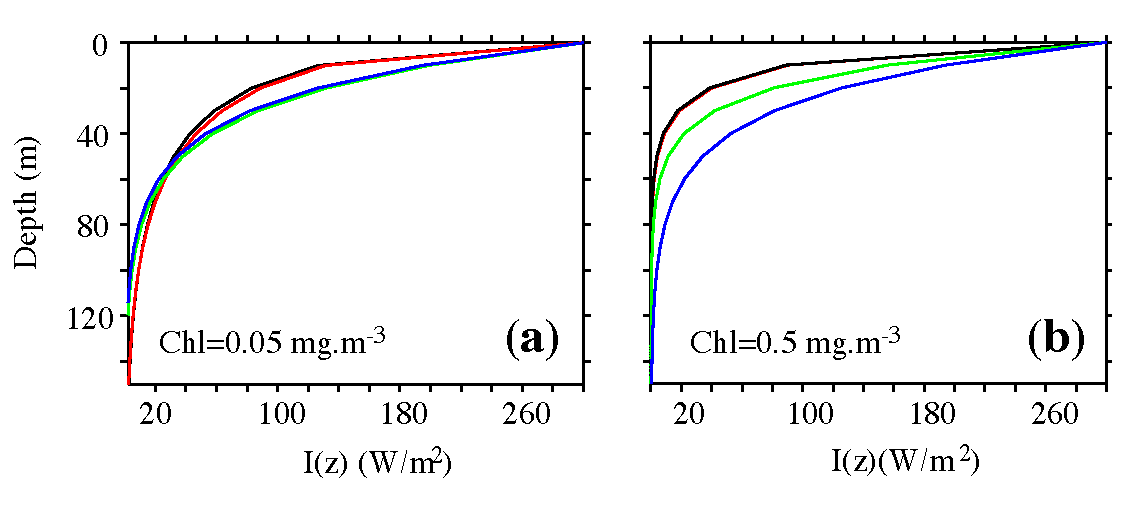
\includegraphics[width=1.0\textwidth]{./TexFiles/Figures/Fig_TRA_Irradiance.pdf}
\caption{ 	 \label{Fig_traqsr_irradiance}
Penetration profile of the downward solar irradiance calculated by four models. 
Two waveband chlorophyll-independent formulation (blue), a chlorophyll-dependent 
monochromatic formulation (green), 4 waveband RGB formulation (red), 
61 waveband Morel (1988) formulation (black) for a chlorophyll concentration of 
(a) Chl=0.05 mg/m$^3$ and (b) Chl=0.5 mg/m$^3$. From \citet{Lengaigne_al_CD07}.}
\end{center}   \end{figure}
%>>>>>>>>>>>>>>>>>>>>>>>>>>>>

% -------------------------------------------------------------------------------------------------------------
%        Bottom Boundary Condition
% -------------------------------------------------------------------------------------------------------------
\subsection   [Bottom Boundary Condition (\textit{trabbc})]
			{Bottom Boundary Condition (\mdl{trabbc})}
\label{TRA_bbc}
%--------------------------------------------nambbc--------------------------------------------------------
\namdisplay{nambbc}
%--------------------------------------------------------------------------------------------------------------
%>>>>>>>>>>>>>>>>>>>>>>>>>>>>
\begin{figure}[!t] 	  \begin{center}
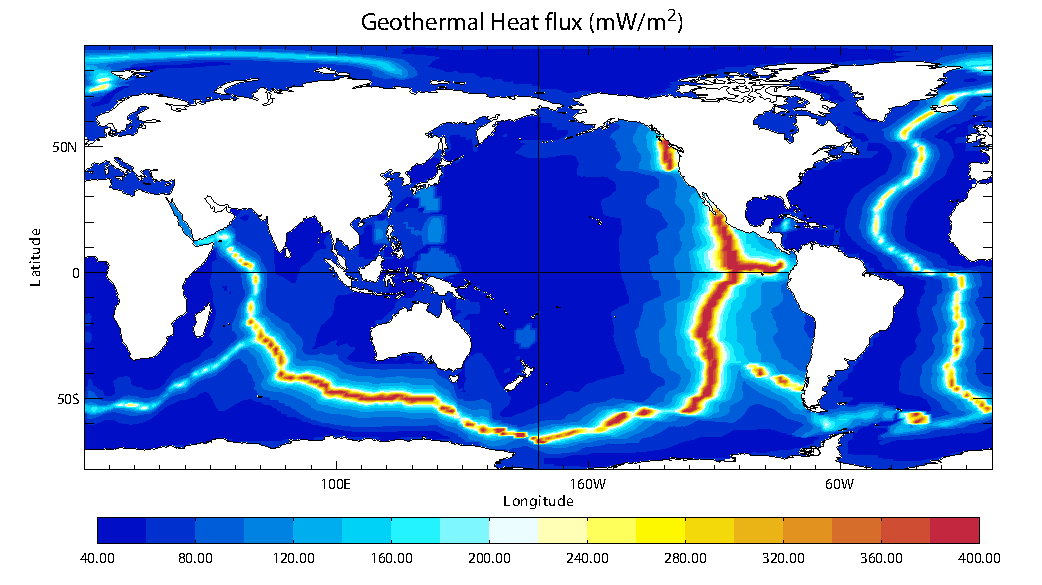
\includegraphics[width=1.0\textwidth]{./TexFiles/Figures/Fig_TRA_geoth.pdf}
\caption{ 	\label{Fig_geothermal}
Geothermal Heat flux (in $mW.m^{-2}$) used by \cite{Emile-Geay_Madec_OS09}.
It is inferred from the age of the sea floor and the formulae of \citet{Stein_Stein_Nat92}.}
\end{center}   \end{figure}
%>>>>>>>>>>>>>>>>>>>>>>>>>>>>

Usually it is assumed that there is no exchange of heat or salt through 
the ocean bottom, $i.e.$ a no flux boundary condition is applied on active 
tracers at the bottom. This is the default option in \NEMO, and it is 
implemented using the masking technique. However, there is a 
non-zero heat flux across the seafloor that is associated with solid 
earth cooling. This flux is weak compared to surface fluxes (a mean 
global value of $\sim0.1\;W/m^2$ \citep{Stein_Stein_Nat92}), but it warms 
systematically the ocean and acts on the densest water masses. 
Taking this flux into account in a global ocean model increases
the deepest overturning cell ($i.e.$ the one associated with the Antarctic 
Bottom Water) by a few Sverdrups  \citep{Emile-Geay_Madec_OS09}. 

Options are defined through the  \ngn{namtra\_bbc} namelist variables.
The presence of geothermal heating is controlled by setting the namelist 
parameter  \np{ln\_trabbc} to true. Then, when \np{nn\_geoflx} is set to 1, 
a constant geothermal heating is introduced whose value is given by the 
\np{nn\_geoflx\_cst}, which is also a namelist parameter. 
When  \np{nn\_geoflx} is set to 2, a spatially varying geothermal heat flux is 
introduced which is provided in the \ifile{geothermal\_heating} NetCDF file 
(Fig.\ref{Fig_geothermal}) \citep{Emile-Geay_Madec_OS09}.

% ================================================================
% Bottom Boundary Layer
% ================================================================
\section  [Bottom Boundary Layer (\mdl{trabbl} - \key{trabbl})]
		{Bottom Boundary Layer (\mdl{trabbl} - \key{trabbl})}
\label{TRA_bbl}
%--------------------------------------------nambbl---------------------------------------------------------
\namdisplay{nambbl}
%--------------------------------------------------------------------------------------------------------------

Options are defined through the  \ngn{nambbl} namelist variables.
In a $z$-coordinate configuration, the bottom topography is represented by a 
series of discrete steps. This is not adequate to represent gravity driven 
downslope flows. Such flows arise either downstream of sills such as the Strait of 
Gibraltar or Denmark Strait, where dense water formed in marginal seas flows 
into a basin filled with less dense water, or along the continental slope when dense 
water masses are formed on a continental shelf. The amount of entrainment 
that occurs in these gravity plumes is critical in determining the density 
and volume flux of the densest waters of the ocean, such as Antarctic Bottom Water, 
or North Atlantic Deep Water. $z$-coordinate models tend to overestimate the 
entrainment, because the gravity flow is mixed vertically by convection 
as it goes ''downstairs'' following the step topography, sometimes over a thickness 
much larger than the thickness of the observed gravity plume. A similar problem 
occurs in the $s$-coordinate when the thickness of the bottom level varies rapidly 
downstream of a sill \citep{Willebrand_al_PO01}, and the thickness 
of the plume is not resolved. 

The idea of the bottom boundary layer (BBL) parameterisation, first introduced by 
\citet{Beckmann_Doscher1997}, is to allow a direct communication between 
two adjacent bottom cells at different levels, whenever the densest water is 
located above the less dense water. The communication can be by a diffusive flux
(diffusive BBL), an advective flux (advective BBL), or both. In the current 
implementation of the BBL, only the tracers are modified, not the velocities. 
Furthermore, it only connects ocean bottom cells, and therefore does not include 
all the improvements introduced by \citet{Campin_Goosse_Tel99}.

% -------------------------------------------------------------------------------------------------------------
%        Diffusive BBL
% -------------------------------------------------------------------------------------------------------------
\subsection{Diffusive Bottom Boundary layer (\np{nn\_bbl\_ldf}=1)}
\label{TRA_bbl_diff}

When applying sigma-diffusion (\key{trabbl} defined and \np{nn\_bbl\_ldf} set to 1), 
the diffusive flux between two adjacent cells at the ocean floor is given by 
\begin{equation} \label{Eq_tra_bbl_diff}
{\rm {\bf F}}_\sigma=A_l^\sigma \; \nabla_\sigma T
\end{equation} 
with $\nabla_\sigma$ the lateral gradient operator taken between bottom cells, 
and  $A_l^\sigma$ the lateral diffusivity in the BBL. Following \citet{Beckmann_Doscher1997}, 
the latter is prescribed with a spatial dependence, $i.e.$ in the conditional form
\begin{equation} \label{Eq_tra_bbl_coef}
A_l^\sigma (i,j,t)=\left\{ {\begin{array}{l}
 A_{bbl}  \quad \quad   \mbox{if}  \quad   \nabla_\sigma \rho  \cdot  \nabla H<0 \\ 
 \\
 0\quad \quad \;\,\mbox{otherwise} \\ 
 \end{array}} \right.
\end{equation} 
where $A_{bbl}$ is the BBL diffusivity coefficient, given by the namelist 
parameter \np{rn\_ahtbbl} and usually set to a value much larger 
than the one used for lateral mixing in the open ocean. The constraint in \eqref{Eq_tra_bbl_coef} 
implies that sigma-like diffusion only occurs when the density above the sea floor, at the top of 
the slope, is larger than in the deeper ocean (see green arrow in Fig.\ref{Fig_bbl}). 
In practice, this constraint is applied separately in the two horizontal directions, 
and the density gradient in \eqref{Eq_tra_bbl_coef} is evaluated with the log gradient formulation: 
\begin{equation} \label{Eq_tra_bbl_Drho}
	\nabla_\sigma \rho / \rho = \alpha \,\nabla_\sigma T + \beta   \,\nabla_\sigma S
\end{equation} 
where $\rho$, $\alpha$ and $\beta$ are functions of $\overline{T}^\sigma$, 
$\overline{S}^\sigma$ and $\overline{H}^\sigma$, the along bottom mean temperature, 
salinity and depth, respectively.

% -------------------------------------------------------------------------------------------------------------
%        Advective BBL
% -------------------------------------------------------------------------------------------------------------
\subsection   {Advective Bottom Boundary Layer  (\np{nn\_bbl\_adv}= 1 or 2)}
\label{TRA_bbl_adv}

\sgacomment{"downsloping flow" has been replaced by "downslope flow" in the following
if this is not what is meant then "downwards sloping flow" is also a possibility"}

%>>>>>>>>>>>>>>>>>>>>>>>>>>>>
\begin{figure}[!t] 	\begin{center}
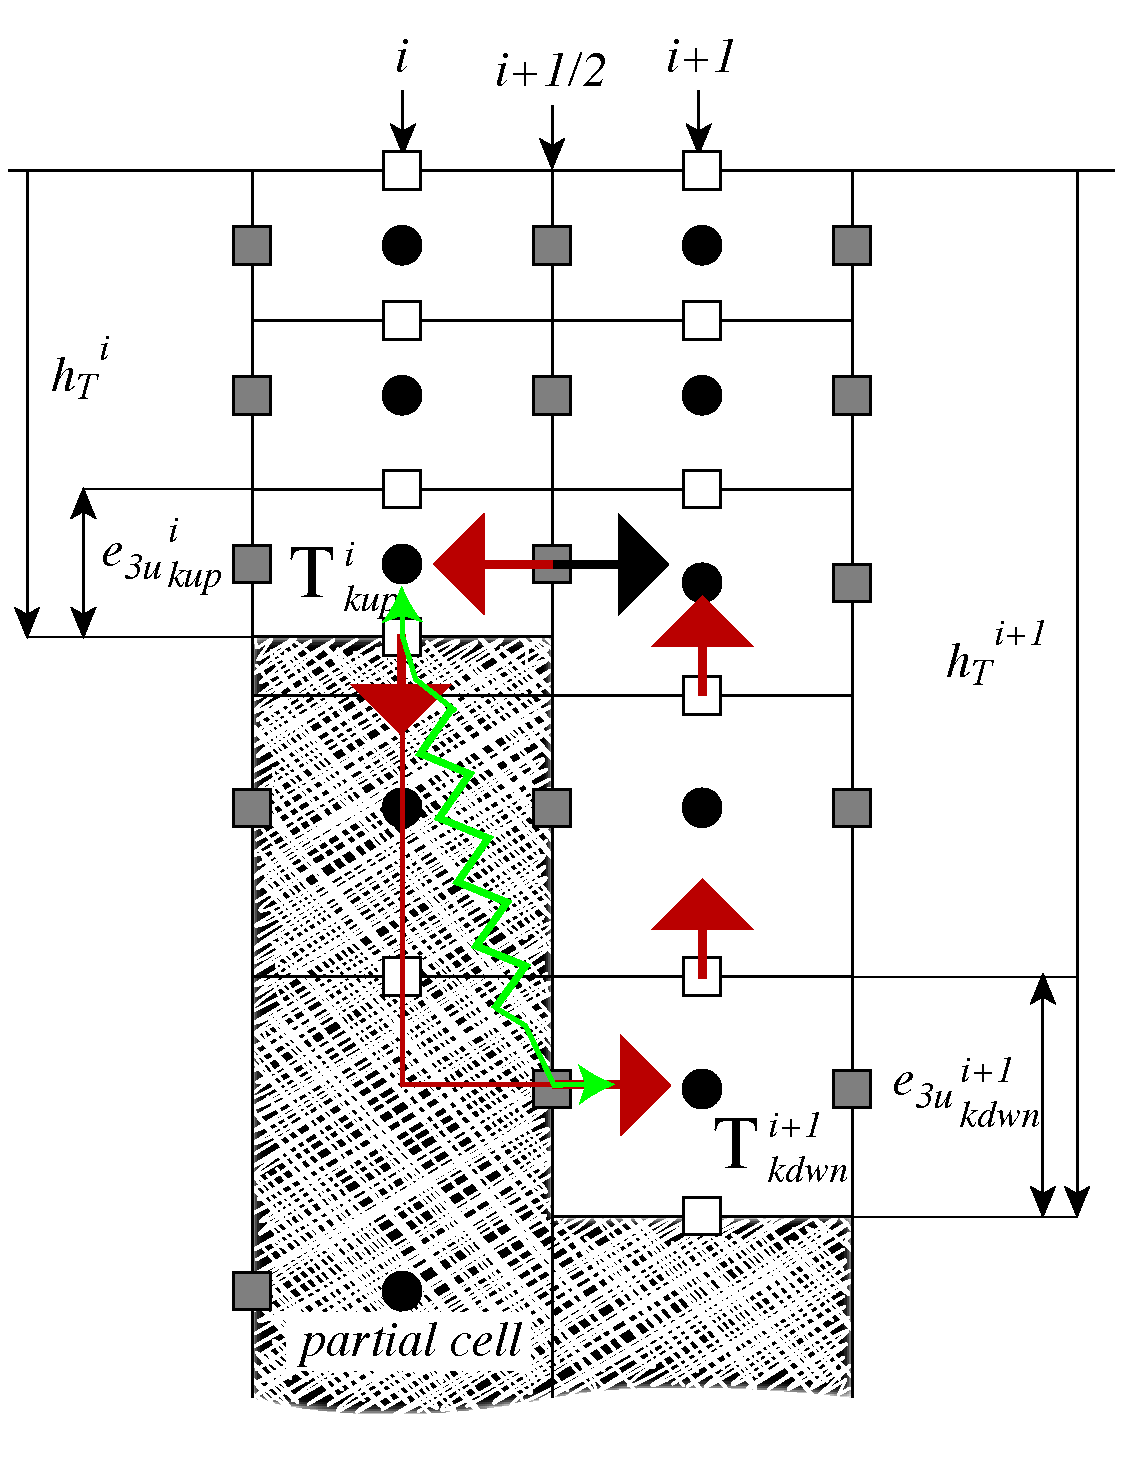
\includegraphics[width=0.7\textwidth]{./TexFiles/Figures/Fig_BBL_adv.pdf}
\caption{ 	\label{Fig_bbl}  
Advective/diffusive Bottom Boundary Layer. The BBL parameterisation is 
activated when $\rho^i_{kup}$ is larger than $\rho^{i+1}_{kdnw}$. 
Red arrows indicate the additional overturning circulation due to the advective BBL. 
The transport of the downslope flow is defined either as the transport of the bottom 
ocean cell (black arrow), or as a function of the along slope density gradient. 
The green arrow indicates the diffusive BBL flux directly connecting $kup$ and $kdwn$
ocean bottom cells.
connection}
\end{center}   \end{figure}
%>>>>>>>>>>>>>>>>>>>>>>>>>>>>


%!!      nn_bbl_adv = 1   use of the ocean velocity as bbl velocity
%!!      nn_bbl_adv = 2   follow Campin and Goosse (1999) implentation
%!!        i.e. transport proportional to the along-slope density gradient

%%%gmcomment   :  this section has to be really written

When applying an advective BBL (\np{nn\_bbl\_adv} = 1 or 2), an overturning 
circulation is added which connects two adjacent bottom grid-points only if dense 
water overlies less dense water on the slope. The density difference causes dense 
water to move down the slope. 

\np{nn\_bbl\_adv} = 1 : the downslope velocity is chosen to be the Eulerian
ocean velocity just above the topographic step (see black arrow in Fig.\ref{Fig_bbl}) 
\citep{Beckmann_Doscher1997}. It is a \textit{conditional advection}, that is, advection
is allowed only if dense water overlies less dense water on the slope ($i.e.$ 
$\nabla_\sigma \rho  \cdot  \nabla H<0$) and if the velocity is directed towards 
greater depth ($i.e.$ $\vect{U}  \cdot  \nabla H>0$).

\np{nn\_bbl\_adv} = 2 : the downslope velocity is chosen to be proportional to $\Delta \rho$,
the density difference between the higher cell and lower cell densities \citep{Campin_Goosse_Tel99}.
The advection is allowed only  if dense water overlies less dense water on the slope ($i.e.$ 
$\nabla_\sigma \rho  \cdot  \nabla H<0$). For example, the resulting transport of the 
downslope flow, here in the $i$-direction (Fig.\ref{Fig_bbl}), is simply given by the 
following expression:
\begin{equation} \label{Eq_bbl_Utr}
 u^{tr}_{bbl} = \gamma \, g \frac{\Delta \rho}{\rho_o}  e_{1u} \; min \left( {e_{3u}}_{kup},{e_{3u}}_{kdwn} \right)
\end{equation}
where $\gamma$, expressed in seconds, is the coefficient of proportionality 
provided as \np{rn\_gambbl}, a namelist parameter, and \textit{kup} and \textit{kdwn} 
are the vertical index of the higher and lower cells, respectively.
The parameter $\gamma$ should take a different value for each bathymetric 
step, but for simplicity, and because no direct estimation of this parameter is 
available, a uniform value has been assumed. The possible values for $\gamma$ 
range between 1 and $10~s$ \citep{Campin_Goosse_Tel99}.  

Scalar properties are advected by this additional transport $( u^{tr}_{bbl}, v^{tr}_{bbl} )$ 
using the upwind scheme. Such a diffusive advective scheme has been chosen 
to mimic the entrainment between the downslope plume and the surrounding 
water at intermediate depths. The entrainment is replaced by the vertical mixing 
implicit in the advection scheme. Let us consider as an example the 
case displayed in Fig.\ref{Fig_bbl} where the density at level $(i,kup)$ is 
larger than the one at level $(i,kdwn)$. The advective BBL scheme
modifies the tracer time tendency of the ocean cells near the 
topographic step by the downslope flow \eqref{Eq_bbl_dw}, 
the horizontal \eqref{Eq_bbl_hor}  and the upward \eqref{Eq_bbl_up} 
return flows as follows: 
\begin{align} 
\partial_t T^{do}_{kdw} &\equiv \partial_t T^{do}_{kdw}
                                     +  \frac{u^{tr}_{bbl}}{{b_t}^{do}_{kdw}}  \left( T^{sh}_{kup} - T^{do}_{kdw} \right)  \label{Eq_bbl_dw} \\
%
\partial_t T^{sh}_{kup} &\equiv \partial_t T^{sh}_{kup} 
				   + \frac{u^{tr}_{bbl}}{{b_t}^{sh}_{kup}}   \left( T^{do}_{kup} - T^{sh}_{kup} \right)   \label{Eq_bbl_hor} \\
%
\intertext{and for $k =kdw-1,\;..., \; kup$ :} 
%
\partial_t T^{do}_{k} &\equiv \partial_t S^{do}_{k}
				   + \frac{u^{tr}_{bbl}}{{b_t}^{do}_{k}}   \left( T^{do}_{k+1} - T^{sh}_{k} \right)   \label{Eq_bbl_up}
\end{align}
where $b_t$ is the $T$-cell volume. 

Note that the BBL transport, $( u^{tr}_{bbl}, v^{tr}_{bbl} )$, is available in 
the model outputs. It has to be used to compute the effective velocity 
as well as the effective overturning circulation.

% ================================================================
% Tracer damping
% ================================================================
\section  [Tracer damping (\textit{tradmp})]
		{Tracer damping (\mdl{tradmp})}
\label{TRA_dmp}
%--------------------------------------------namtra_dmp-------------------------------------------------
\namdisplay{namtra_dmp}
%--------------------------------------------------------------------------------------------------------------

In some applications it can be useful to add a Newtonian damping term 
into the temperature and salinity equations:
\begin{equation} \label{Eq_tra_dmp}
\begin{split}
 \frac{\partial T}{\partial t}=\;\cdots \;-\gamma \,\left( {T-T_o } \right)  \\
 \frac{\partial S}{\partial t}=\;\cdots \;-\gamma \,\left( {S-S_o } \right) 
 \end{split}
 \end{equation} 
where $\gamma$ is the inverse of a time scale, and $T_o$ and $S_o$ 
are given temperature and salinity fields (usually a climatology). 
Options are defined through the  \ngn{namtra\_dmp} namelist variables.
The restoring term is added when the namelist parameter \np{ln\_tradmp} is set to true. 
It also requires that both \np{ln\_tsd\_init} and \np{ln\_tsd\_tradmp} are set to true
in \textit{namtsd} namelist as well as \np{sn\_tem} and \np{sn\_sal} structures are 
correctly set  ($i.e.$ that $T_o$ and $S_o$ are provided in input files and read 
using \mdl{fldread}, see \S\ref{SBC_fldread}). 
The restoring coefficient $\gamma$ is a three-dimensional array read in during the \rou{tra\_dmp\_init} routine. The file name is specified by the namelist variable \np{cn\_resto}. The DMP\_TOOLS tool is provided to allow users to generate the netcdf file.

The two main cases in which \eqref{Eq_tra_dmp} is used are \textit{(a)} 
the specification of the boundary conditions along artificial walls of a 
limited domain basin and \textit{(b)} the computation of the velocity 
field associated with a given $T$-$S$ field (for example to build the 
initial state of a prognostic simulation, or to use the resulting velocity 
field for a passive tracer study). The first case applies to regional 
models that have artificial walls instead of open boundaries. 
In the vicinity of these walls, $\gamma$ takes large values (equivalent to 
a time scale of a few days) whereas it is zero in the interior of the 
model domain. The second case corresponds to the use of the robust 
diagnostic method \citep{Sarmiento1982}. It allows us to find the velocity 
field consistent with the model dynamics whilst having a $T$, $S$ field 
close to a given climatological field ($T_o$, $S_o$). 

The robust diagnostic method is very efficient in preventing temperature 
drift in intermediate waters but it produces artificial sources of heat and salt 
within the ocean. It also has undesirable effects on the ocean convection. 
It tends to prevent deep convection and subsequent deep-water formation, 
by stabilising the water column too much.

The namelist parameter \np{nn\_zdmp} sets whether the damping should be applied in the whole water column or only below the mixed layer (defined either on a density or $S_o$ criterion). It is common to set the damping to zero in the mixed layer as the adjustment time scale is short here \citep{Madec_al_JPO96}.

\subsection[DMP\_TOOLS]{Generating resto.nc using DMP\_TOOLS}

DMP\_TOOLS can be used to generate a netcdf file containing the restoration coefficient $\gamma$. Note that in order to maintain bit comparison with previous NEMO versions DMP\_TOOLS must be compiled and run on the same machine as the NEMO model. A mesh\_mask.nc file for the model configuration is required as an input. This can be generated by carrying out a short model run with the namelist parameter \np{nn\_msh} set to 1. The namelist parameter \np{ln\_tradmp} will also need to be set to .false. for this to work. The \nl{nam\_dmp\_create} namelist in the DMP\_TOOLS directory is used to specify options for the restoration coefficient.

%--------------------------------------------nam_dmp_create-------------------------------------------------
\namdisplay{nam_dmp_create}
%-------------------------------------------------------------------------------------------------------

\np{cp\_cfg}, \np{cp\_cpz}, \np{jp\_cfg} and \np{jperio} specify the model configuration being used and should be the same as specified in \nl{namcfg}. The variable \nl{lzoom} is used to specify that the damping is being used as in case \textit{a} above to provide boundary conditions to a zoom configuration. In the case of the arctic or antarctic zoom configurations this includes some specific treatment. Otherwise damping is applied to the 6 grid points along the ocean boundaries. The open boundaries are specified by the variables \np{lzoom\_n}, \np{lzoom\_e}, \np{lzoom\_s}, \np{lzoom\_w} in the \nl{nam\_zoom\_dmp} name list.

The remaining switch namelist variables determine the spatial variation of the restoration coefficient in non-zoom configurations. \np{ln\_full\_field} specifies that newtonian damping should be applied to the whole model domain. \np{ln\_med\_red\_seas} specifies grid specific restoration coefficients in the Mediterranean Sea for the ORCA4, ORCA2 and ORCA05 configurations. If \np{ln\_old\_31\_lev\_code} is set then the depth variation of the coeffients will be specified as a function of the model number. This option is included to allow backwards compatability of the ORCA2 reference configurations with previous model versions. \np{ln\_coast} specifies that the restoration coefficient should be reduced near to coastlines. This option only has an effect if \np{ln\_full\_field} is true. \np{ln\_zero\_top\_layer} specifies that the restoration coefficient should be zero in the surface layer. Finally \np{ln\_custom} specifies that the custom module will be called. This module is contained in the file custom.F90 and can be edited by users. For example damping could be applied in a specific region.

The restoration coefficient can be set to zero in equatorial regions by specifying a positive value of \np{nn\_hdmp}. Equatorward of this latitude the restoration coefficient will be zero with a smooth transition to the full values of a 10$^{\circ}$ latitud band. This is often used because of the short adjustment time scale in the equatorial region \citep{Reverdin1991, Fujio1991, Marti_PhD92}. The time scale associated with the damping depends on the depth as a hyperbolic tangent, with \np{rn\_surf} as surface value, \np{rn\_bot} as bottom value and a transition depth of \np{rn\_dep}.  

% ================================================================
% Tracer time evolution
% ================================================================
\section  [Tracer time evolution (\textit{tranxt})]
		{Tracer time evolution (\mdl{tranxt})}
\label{TRA_nxt}
%--------------------------------------------namdom-----------------------------------------------------
\namdisplay{namdom}
%--------------------------------------------------------------------------------------------------------------

Options are defined through the  \ngn{namdom} namelist variables.
The general framework for tracer time stepping is a modified leap-frog scheme 
\citep{Leclair_Madec_OM09}, $i.e.$ a three level centred time scheme associated 
with a Asselin time filter (cf. \S\ref{STP_mLF}):
\begin{equation} \label{Eq_tra_nxt}
\begin{aligned}
(e_{3t}T)^{t+\rdt} &= (e_{3t}T)_f^{t-\rdt} &+ 2 \, \rdt  \,e_{3t}^t\ \text{RHS}^t &	\\
\\
(e_{3t}T)_f^t  \;\ \quad &= (e_{3t}T)^t \;\quad 
                                    &+\gamma \,\left[ {(e_{3t}T)_f^{t-\rdt} -2(e_{3t}T)^t+(e_{3t}T)^{t+\rdt}} \right] &  \\
                                 & &- \gamma\,\rdt \, \left[ Q^{t+\rdt/2} -  Q^{t-\rdt/2} \right]  &                      
\end{aligned}
\end{equation} 
where RHS is the right hand side of the temperature equation, 
the subscript $f$ denotes filtered values, $\gamma$ is the Asselin coefficient,
and $S$ is the total forcing applied on $T$ ($i.e.$ fluxes plus content in mass exchanges). 
$\gamma$ is initialized as \np{rn\_atfp} (\textbf{namelist} parameter). 
Its default value is \np{rn\_atfp}=$10^{-3}$. Note that the forcing correction term in the filter
is not applied in linear free surface (\jp{lk\_vvl}=false) (see \S\ref{TRA_sbc}.
Not also that in constant volume case, the time stepping is performed on $T$, 
not on its content, $e_{3t}T$.

When the vertical mixing is solved implicitly, the update of the \textit{next} tracer 
fields is done in module \mdl{trazdf}. In this case only the swapping of arrays 
and the Asselin filtering is done in the \mdl{tranxt} module.

In order to prepare for the computation of the \textit{next} time step, 
a swap of tracer arrays is performed: $T^{t-\rdt} = T^t$ and $T^t = T_f$. 

% ================================================================
% Equation of State (eosbn2) 
% ================================================================
\section  [Equation of State (\textit{eosbn2}) ]
		{Equation of State (\mdl{eosbn2}) }
\label{TRA_eosbn2}
%--------------------------------------------nameos-----------------------------------------------------
\namdisplay{nameos}
%--------------------------------------------------------------------------------------------------------------

% -------------------------------------------------------------------------------------------------------------
%        Equation of State
% -------------------------------------------------------------------------------------------------------------
\subsection{Equation Of Seawater (\np{nn\_eos} = -1, 0, or 1)}
\label{TRA_eos}

The Equation Of Seawater (EOS) is an empirical nonlinear thermodynamic relationship 
linking seawater density, $\rho$, to a number of state variables, 
most typically temperature, salinity and pressure. 
Because density gradients control the pressure gradient force through the hydrostatic balance, 
the equation of state provides a fundamental bridge between the distribution of active tracers 
and the fluid dynamics. Nonlinearities of the EOS are of major importance, in particular 
influencing the circulation through determination of the static stability below the mixed layer, 
thus controlling rates of exchange between the atmosphere  and the ocean interior \citep{Roquet_JPO2015}. 
Therefore an accurate EOS based on either the 1980 equation of state (EOS-80, \cite{UNESCO1983}) 
or TEOS-10 \citep{TEOS10} standards should be used anytime a simulation of the real 
ocean circulation is attempted \citep{Roquet_JPO2015}. 
The use of TEOS-10 is highly recommended because 
\textit{(i)} it is the new official EOS, 
\textit{(ii)} it is more accurate, being based on an updated database of laboratory measurements, and 
\textit{(iii)} it uses Conservative Temperature and Absolute Salinity (instead of potential temperature 
and practical salinity for EOS-980, both variables being more suitable for use as model variables 
\citep{TEOS10, Graham_McDougall_JPO13}. 
EOS-80 is an obsolescent feature of the NEMO system, kept only for backward compatibility.
For process studies, it is often convenient to use an approximation of the EOS. To that purposed, 
a simplified EOS (S-EOS) inspired by \citet{Vallis06} is also available.

In the computer code, a density anomaly, $d_a= \rho / \rho_o - 1$, 
is computed, with $\rho_o$ a reference density. Called \textit{rau0} 
in the code, $\rho_o$ is set in \mdl{phycst} to a value of $1,026~Kg/m^3$. 
This is a sensible choice for the reference density used in a Boussinesq ocean 
climate model, as, with the exception of only a small percentage of the ocean, 
density in the World Ocean varies by no more than 2$\%$ from that value \citep{Gill1982}.

Options are defined through the  \ngn{nameos} namelist variables, and in particular \np{nn\_eos} 
which controls the EOS used (=-1 for TEOS10 ; =0 for EOS-80 ; =1 for S-EOS).
\begin{description}

\item[\np{nn\_eos}$=-1$] the polyTEOS10-bsq equation of seawater \citep{Roquet_OM2015} is used.  
The accuracy of this approximation is comparable to the TEOS-10 rational function approximation, 
but it is optimized for a boussinesq fluid and the polynomial expressions have simpler 
and more computationally efficient expressions for their derived quantities 
which make them more adapted for use in ocean models. 
Note that a slightly higher precision polynomial form is now used replacement of the TEOS-10 
rational function approximation for hydrographic data analysis  \citep{TEOS10}. 
A key point is that conservative state variables are used: 
Absolute Salinity (unit: g/kg, notation: $S_A$) and Conservative Temperature (unit: $\degres C$, notation: $\Theta$).
The pressure in decibars is approximated by the depth in meters. 
With TEOS10, the specific heat capacity of sea water, $C_p$, is a constant. It is set to 
$C_p=3991.86795711963~J\,Kg^{-1}\,\degres K^{-1}$, according to \citet{TEOS10}.

Choosing polyTEOS10-bsq implies that the state variables used by the model are 
$\Theta$ and $S_A$. In particular, the initial state deined by the user have to be given as 
\textit{Conservative} Temperature and \textit{Absolute} Salinity. 
In addition, setting \np{ln\_useCT} to \textit{true} convert the Conservative SST to potential SST 
prior to either computing the air-sea and ice-sea fluxes (forced mode) 
or sending the SST field to the atmosphere (coupled mode).

\item[\np{nn\_eos}$=0$] the polyEOS80-bsq equation of seawater is used.
It takes the same polynomial form as the polyTEOS10, but the coefficients have been optimized 
to accurately fit EOS80 (Roquet, personal comm.). The state variables used in both the EOS80 
and the ocean model are: 
the Practical Salinity ((unit: psu, notation: $S_p$)) and Potential Temperature (unit: $\degres C$, notation: $\theta$).
The pressure in decibars is approximated by the depth in meters.  
With thsi EOS, the specific heat capacity of sea water, $C_p$, is a function of temperature, 
salinity and pressure \citep{UNESCO1983}. Nevertheless, a severe assumption is made in order to 
have a heat content ($C_p T_p$) which is conserved by the model: $C_p$ is set to a constant 
value, the TEOS10 value. 
 
\item[\np{nn\_eos}$=1$] a simplified EOS (S-EOS) inspired by \citet{Vallis06} is chosen, 
the coefficients of which has been optimized to fit the behavior of TEOS10 (Roquet, personal comm.) 
(see also \citet{Roquet_JPO2015}). It provides a simplistic linear representation of both 
cabbeling and thermobaricity effects which is enough for a proper treatment of the EOS 
in theoretical studies \citep{Roquet_JPO2015}.
With such an equation of state there is no longer a distinction between 
\textit{conservative} and \textit{potential} temperature, as well as between \textit{absolute} 
and \textit{practical} salinity.
S-EOS takes the following expression:
\begin{equation} \label{Eq_tra_S-EOS}
\begin{split}
  d_a(T,S,z)  =  ( & - a_0 \; ( 1 + 0.5 \; \lambda_1 \; T_a + \mu_1 \; z ) * T_a  \\
                                & + b_0 \; ( 1 - 0.5 \; \lambda_2 \; S_a - \mu_2 \; z ) * S_a  \\
                                & - \nu \; T_a \; S_a \;  ) \; / \; \rho_o                     \\
  with \ \  T_a = T-10  \; ;  & \;  S_a = S-35  \; ;\;  \rho_o = 1026~Kg/m^3
\end{split}
\end{equation} 
where the computer name of the coefficients as well as their standard value are given in \ref{Tab_SEOS}.
In fact, when choosing S-EOS, various approximation of EOS can be specified simply by changing 
the associated coefficients. 
Setting to zero the two thermobaric coefficients ($\mu_1$, $\mu_2$) remove thermobaric effect from S-EOS.
setting to zero the three cabbeling coefficients ($\lambda_1$, $\lambda_2$, $\nu$) remove cabbeling effect from S-EOS.
Keeping non-zero value to $a_0$ and $b_0$ provide a linear EOS function of T and S.

\end{description}


%>>>>>>>>>>>>>>>>>>>>>>>>>>>>
\begin{table}[!tb]
\begin{center} \begin{tabular}{|p{26pt}|p{72pt}|p{56pt}|p{136pt}|}
\hline
coeff.	& computer name   & S-EOS		&  description		                  \\ \hline
$a_0$       & \np{nn\_a0}     & 1.6550 $10^{-1}$ &  linear thermal expansion coeff. 	\\ \hline
$b_0$	      & \np{nn\_b0} 	   & 7.6554 $10^{-1}$ &  linear haline  expansion coeff. 	\\ \hline
$\lambda_1$	& \np{nn\_lambda1}& 5.9520 $10^{-2}$ &  cabbeling coeff. in $T^2$ 	      \\ \hline
$\lambda_2$	& \np{nn\_lambda2}& 5.4914 $10^{-4}$ &  cabbeling coeff. in $S^2$	 	   \\ \hline
$\nu$       & \np{nn\_nu}     & 2.4341 $10^{-3}$ &  cabbeling coeff. in $T \, S$ 	   \\ \hline
$\mu_1$     & \np{nn\_mu1} 	& 1.4970 $10^{-4}$ &  thermobaric coeff. in T    	   \\ \hline
$\mu_2$     & \np{nn\_mu2} 	& 1.1090 $10^{-5}$ &  thermobaric coeff. in S   	      \\ \hline
\end{tabular}
\caption{ \label{Tab_SEOS}
Standard value of S-EOS coefficients. }
\end{center}
\end{table}
%>>>>>>>>>>>>>>>>>>>>>>>>>>>>


% -------------------------------------------------------------------------------------------------------------
%        Brunt-Vais\"{a}l\"{a} Frequency
% -------------------------------------------------------------------------------------------------------------
\subsection{Brunt-Vais\"{a}l\"{a} Frequency (\np{nn\_eos} = 0, 1 or 2)}
\label{TRA_bn2}

An accurate computation of the ocean stability (i.e. of $N$, the brunt-Vais\"{a}l\"{a}
 frequency) is of paramount importance as determine the ocean stratification and 
 is used in several ocean parameterisations (namely TKE, GLS, Richardson number dependent 
 vertical diffusion, enhanced vertical diffusion, non-penetrative convection, tidal mixing 
 parameterisation, iso-neutral diffusion). In particular, $N^2$ has to be computed at the local pressure 
 (pressure in decibar being approximated by the depth in meters). The expression for $N^2$ 
 is given by: 
\begin{equation} \label{Eq_tra_bn2}
N^2 =	\frac{g}{e_{3w}} \left(   \beta \;\delta_{k+1/2}[S] - \alpha \;\delta_{k+1/2}[T]   \right)
\end{equation} 
where $(T,S) = (\Theta, S_A)$ for TEOS10, $= (\theta, S_p)$ for TEOS-80, or $=(T,S)$ for S-EOS, 
and, $\alpha$ and $\beta$ are the thermal and haline expansion coefficients. 
The coefficients are a polynomial function of temperature, salinity and depth which expression 
depends on the chosen EOS. They are computed through \textit{eos\_rab}, a \textsc{Fortran} 
function that can be found in \mdl{eosbn2}.


% -------------------------------------------------------------------------------------------------------------
%        Potential Energy     
% -------------------------------------------------------------------------------------------------------------
%\subsection{Potential Energy anomalies}
%\label{TRA_bn2}

%    =====>>>>> TO BE written
%

% -------------------------------------------------------------------------------------------------------------
%        Freezing Point of Seawater
% -------------------------------------------------------------------------------------------------------------
\subsection   [Freezing Point of Seawater]
			{Freezing Point of Seawater}
\label{TRA_fzp}

The freezing point of seawater is a function of salinity and pressure \citep{UNESCO1983}:
\begin{equation} \label{Eq_tra_eos_fzp}
   \begin{split}
T_f (S,p) = \left( -0.0575 + 1.710523 \;10^{-3} \, \sqrt{S} 
						     -  2.154996 \;10^{-4} \,S  \right) \ S    \\
               - 7.53\,10^{-3} \ \ p 
   \end{split}
\end{equation}

\eqref{Eq_tra_eos_fzp} is only used to compute the potential freezing point of 
sea water ($i.e.$ referenced to the surface $p=0$), thus the pressure dependent 
terms in \eqref{Eq_tra_eos_fzp} (last term) have been dropped. The freezing
point is computed through \textit{eos\_fzp}, a \textsc{Fortran} function that can be found 
in \mdl{eosbn2}.  

% ================================================================
% Horizontal Derivative in zps-coordinate 
% ================================================================
\section  [Horizontal Derivative in \textit{zps}-coordinate (\textit{zpshde})]
		{Horizontal Derivative in \textit{zps}-coordinate (\mdl{zpshde})}
\label{TRA_zpshde}

\gmcomment{STEVEN: to be consistent with earlier discussion of differencing and averaging operators, I've changed "derivative" to "difference" and "mean" to "average"}

With partial bottom cells (\np{ln\_zps}=true), in general, tracers in horizontally 
adjacent cells live at different depths. Horizontal gradients of tracers are needed 
for horizontal diffusion (\mdl{traldf} module) and for the hydrostatic pressure 
gradient (\mdl{dynhpg} module) to be active. 
\gmcomment{STEVEN from gm : question: not sure of  what -to be active- means}
Before taking horizontal gradients between the tracers next to the bottom, a linear 
interpolation in the vertical is used to approximate the deeper tracer as if it actually 
lived at the depth of the shallower tracer point (Fig.~\ref{Fig_Partial_step_scheme}). 
For example, for temperature in the $i$-direction the needed interpolated 
temperature, $\widetilde{T}$, is:

%>>>>>>>>>>>>>>>>>>>>>>>>>>>>
\begin{figure}[!p] 	 \begin{center}
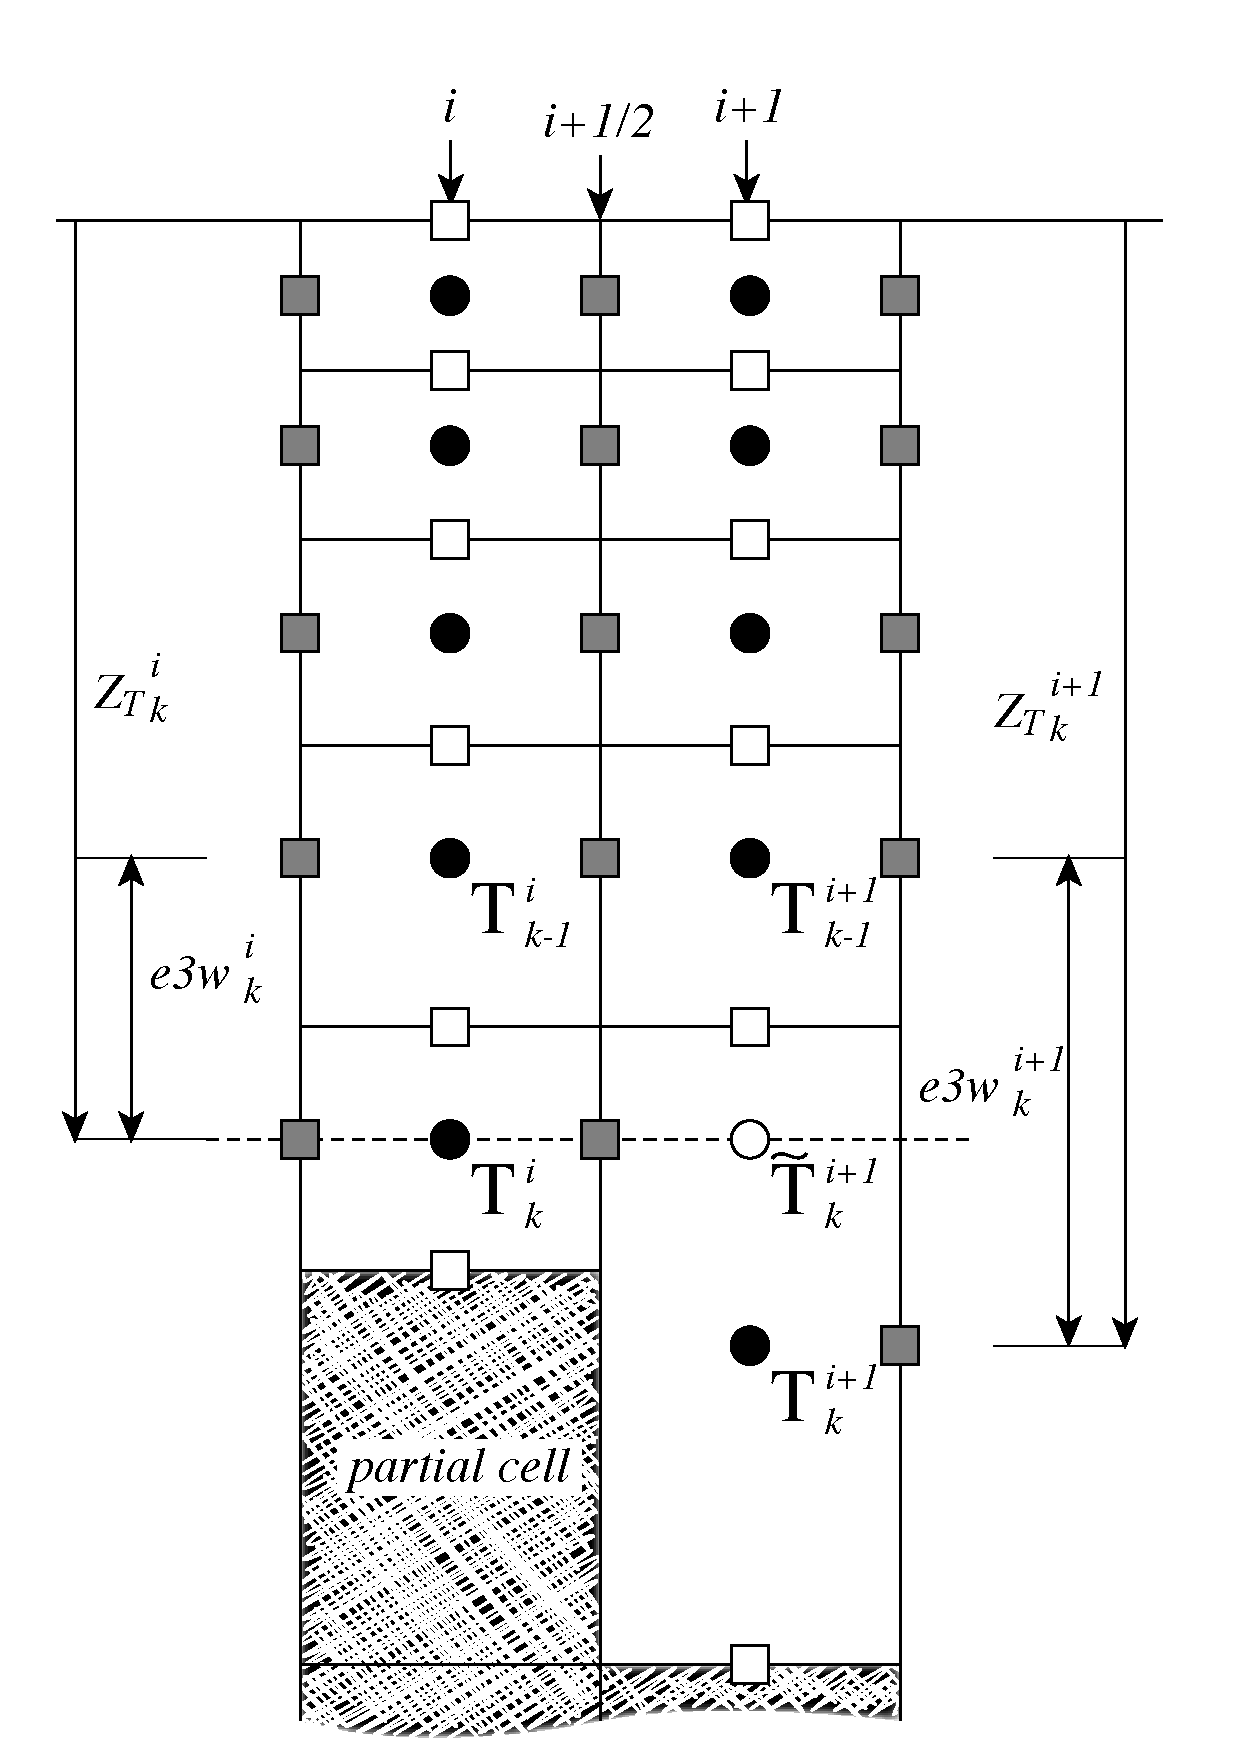
\includegraphics[width=0.9\textwidth]{./TexFiles/Figures/Partial_step_scheme.pdf}
\caption{ 	\label{Fig_Partial_step_scheme} 
Discretisation of the horizontal difference and average of tracers in the $z$-partial 
step coordinate (\np{ln\_zps}=true) in the case $( e3w_k^{i+1} - e3w_k^i  )>0$. 
A linear interpolation is used to estimate $\widetilde{T}_k^{i+1}$, the tracer value 
at the depth of the shallower tracer point of the two adjacent bottom $T$-points. 
The horizontal difference is then given by: $\delta _{i+1/2} T_k=  \widetilde{T}_k^{\,i+1} -T_k^{\,i}$ 
and the average by: $\overline{T}_k^{\,i+1/2}= ( \widetilde{T}_k^{\,i+1/2} - T_k^{\,i} ) / 2$.  }
\end{center}   \end{figure}
%>>>>>>>>>>>>>>>>>>>>>>>>>>>>
\begin{equation*}
\widetilde{T}= \left\{  \begin{aligned}  
&T^{\,i+1}      -\frac{ \left( e_{3w}^{i+1} -e_{3w}^i \right)}{ e_{3w}^{i+1} }\;\delta _k T^{i+1}	
 								&& \quad\text{if  $\ e_{3w}^{i+1} \geq e_{3w}^i$   } 	\\
										\\
&T^{\,i} \ \ \ \,+\frac{ \left( e_{3w}^{i+1} -e_{3w}^i \right) }{e_{3w}^i       }\;\delta _k T^{i+1}
			 					&& \quad\text{if  $\ e_{3w}^{i+1}    <   e_{3w}^i$   } 
            \end{aligned}   \right.
\end{equation*}
and the resulting forms for the horizontal difference and the horizontal average 
value of $T$ at a $U$-point are: 
\begin{equation} \label{Eq_zps_hde}
\begin{aligned}
 \delta _{i+1/2} T= 	\begin{cases}
\ \ \ \widetilde {T}\quad\ -T^i	 	& \ \ \quad\quad\text{if  $\ e_{3w}^{i+1} \geq e_{3w}^i$ } \\
										\\
\ \ \ T^{\,i+1}-\widetilde{T}		& \ \ \quad\quad\text{if  $\ e_{3w}^{i+1}    <   e_{3w}^i$   } 
            		\end{cases}     \\
\\
\overline {T}^{\,i+1/2} \ = 	\begin{cases}
( \widetilde {T}\ \ \;\,-T^{\,i})	 / 2	& \;\ \ \quad\text{if  $\ e_{3w}^{i+1} \geq e_{3w}^i$ } \\
										\\
( T^{\,i+1}-\widetilde{T} ) / 2		& \;\ \ \quad\text{if  $\ e_{3w}^{i+1}    <   e_{3w}^i$   } 
            \end{cases}
\end{aligned}
\end{equation}

The computation of horizontal derivative of tracers as well as of density is 
performed once for all at each time step in \mdl{zpshde} module and stored 
in shared arrays to be used when needed. It has to be emphasized that the 
procedure used to compute the interpolated density, $\widetilde{\rho}$, is not 
the same as that used for $T$ and $S$. Instead of forming a linear approximation 
of density, we compute $\widetilde{\rho }$ from the interpolated values of $T$ 
and $S$, and the pressure at a $u$-point (in the equation of state pressure is 
approximated by depth, see \S\ref{TRA_eos} ) : 
\begin{equation} \label{Eq_zps_hde_rho}
\widetilde{\rho } = \rho ( {\widetilde{T},\widetilde {S},z_u }) 
\quad \text{where }\  z_u = \min \left( {z_T^{i+1} ,z_T^i } \right)
\end{equation} 

This is a much better approximation as the variation of $\rho$ with depth (and 
thus pressure) is highly non-linear with a true equation of state and thus is badly 
approximated with a linear interpolation. This approximation is used to compute 
both the horizontal pressure gradient (\S\ref{DYN_hpg}) and the slopes of neutral 
surfaces (\S\ref{LDF_slp})

Note that in almost all the advection schemes presented in this Chapter, both 
averaging and differencing operators appear. Yet \eqref{Eq_zps_hde} has not 
been used in these schemes: in contrast to diffusion and pressure gradient 
computations, no correction for partial steps is applied for advection. The main 
motivation is to preserve the domain averaged mean variance of the advected 
field when using the $2^{nd}$ order centred scheme. Sensitivity of the advection 
schemes to the way horizontal averages are performed in the vicinity of partial 
cells should be further investigated in the near future.
%%%
\gmcomment{gm :   this last remark has to be done}
%%%
			% Tracer advection/diffusion equation

% ================================================================
% Chapter � Ocean Dynamics (DYN)
% ================================================================
\chapter{Ocean Dynamics (DYN)}
\label{DYN}
\minitoc

% add a figure for  dynvor ens, ene latices

%\vspace{2.cm}
$\ $\newline      %force an empty line

Using the representation described in Chapter \ref{DOM}, several semi-discrete 
space forms of the dynamical equations are available depending on the vertical 
coordinate used and on the conservation properties of the vorticity term. In all 
the equations presented here, the masking has been omitted for simplicity. 
One must be aware that all the quantities are masked fields and that each time an
average or difference operator is used, the resulting field is multiplied by a mask.

The prognostic ocean dynamics equation can be summarized as follows:
\begin{equation*}
\text{NXT} = \dbinom	{\text{VOR} + \text{KEG} + \text {ZAD} }
						{\text{COR} + \text{ADV}                       }
			+ \text{HPG} + \text{SPG} + \text{LDF} + \text{ZDF}
\end{equation*}
NXT stands for next, referring to the time-stepping. The first group of terms on 
the rhs of this equation corresponds to the Coriolis and advection 
terms that are decomposed into either a vorticity part (VOR), a kinetic energy part (KEG) 
and a vertical advection part (ZAD) in the vector invariant formulation, or a Coriolis 
and advection part (COR+ADV) in the flux formulation. The terms following these 
are the pressure gradient contributions (HPG, Hydrostatic Pressure Gradient, 
and SPG, Surface Pressure Gradient); and contributions from lateral diffusion 
(LDF) and vertical diffusion (ZDF), which are added to the rhs in the \mdl{dynldf} 
and \mdl{dynzdf} modules. The vertical diffusion term includes the surface and 
bottom stresses. The external forcings and parameterisations require complex 
inputs (surface wind stress calculation using bulk formulae, estimation of mixing 
coefficients) that are carried out in modules SBC, LDF and ZDF and are described 
in Chapters \ref{SBC}, \ref{LDF} and \ref{ZDF}, respectively. 

In the present chapter we also describe the diagnostic equations used to compute 
the horizontal divergence, curl of the velocities (\emph{divcur} module) and 
the vertical velocity (\emph{wzvmod} module).

The different options available to the user are managed by namelist variables. 
For term \textit{ttt} in the momentum equations, the logical namelist variables are \textit{ln\_dynttt\_xxx}, 
where \textit{xxx} is a 3 or 4 letter acronym corresponding to each optional scheme. 
If a CPP key is used for this term its name is \textbf{key\_ttt}. The corresponding 
code can be found in the \textit{dynttt\_xxx} module in the DYN directory, and it is 
usually computed in the \textit{dyn\_ttt\_xxx} subroutine.

The user has the option of extracting and outputting each tendency term from the
3D momentum equations (\key{trddyn} defined), as described in 
Chap.\ref{MISC}.  Furthermore, the tendency terms associated with the 2D 
barotropic vorticity balance (when \key{trdvor} is defined) can be derived from the 
3D terms.
%%%
\gmcomment{STEVEN: not quite sure I've got the sense of the last sentence. does 
MISC correspond to "extracting tendency terms" or "vorticity balance"?}

$\ $\newline    % force a new ligne

% ================================================================
% Sea Surface Height evolution & Diagnostics variables
% ================================================================
\section{Sea surface height and diagnostic variables ($\eta$, $\zeta$, $\chi$, $w$)}
\label{DYN_divcur_wzv}

%--------------------------------------------------------------------------------------------------------------
%           Horizontal divergence and relative vorticity
%--------------------------------------------------------------------------------------------------------------
\subsection   [Horizontal divergence and relative vorticity (\textit{divcur})]
			{Horizontal divergence and relative vorticity (\mdl{divcur})}
\label{DYN_divcur}

The vorticity is defined at an $f$-point ($i.e.$ corner point) as follows:
\begin{equation} \label{Eq_divcur_cur}
\zeta =\frac{1}{e_{1f}\,e_{2f} }\left( {\;\delta _{i+1/2} \left[ {e_{2v}\;v} \right]
						        -\delta _{j+1/2} \left[ {e_{1u}\;u} \right]\;} \right)
\end{equation} 

The horizontal divergence is defined at a $T$-point. It is given by:
\begin{equation} \label{Eq_divcur_div}
\chi =\frac{1}{e_{1t}\,e_{2t}\,e_{3t} }
		\left( {\delta _i \left[ {e_{2u}\,e_{3u}\,u} \right]
		       +\delta _j \left[ {e_{1v}\,e_{3v}\,v} \right]} \right)
\end{equation} 

Note that although the vorticity has the same discrete expression in $z$- 
and $s$-coordinates, its physical meaning is not identical. $\zeta$ is a pseudo 
vorticity along $s$-surfaces (only pseudo because $(u,v)$ are still defined along 
geopotential surfaces, but are not necessarily defined at the same depth).

The vorticity and divergence at the \textit{before} step are used in the computation 
of the horizontal diffusion of momentum. Note that because they have been 
calculated prior to the Asselin filtering of the \textit{before} velocities, the 
\textit{before} vorticity and divergence arrays must be included in the restart file 
to ensure perfect restartability. The vorticity and divergence at the \textit{now} 
time step are used for the computation of the nonlinear advection and of the 
vertical velocity respectively. 

%--------------------------------------------------------------------------------------------------------------
%           Sea Surface Height evolution
%--------------------------------------------------------------------------------------------------------------
\subsection   [Sea surface height evolution and vertical velocity (\textit{sshwzv})]
			{Horizontal divergence and relative vorticity (\mdl{sshwzv})}
\label{DYN_sshwzv}

The sea surface height is given by :
\begin{equation} \label{Eq_dynspg_ssh}
\begin{aligned}
\frac{\partial \eta }{\partial t}
&\equiv    \frac{1}{e_{1t} e_{2t} }\sum\limits_k { \left\{  \delta _i \left[ {e_{2u}\,e_{3u}\;u} \right]
                                                                                  +\delta _j \left[ {e_{1v}\,e_{3v}\;v} \right]  \right\} } 
           -    \frac{\textit{emp}}{\rho _w }   \\
&\equiv    \sum\limits_k {\chi \ e_{3t}}  -  \frac{\textit{emp}}{\rho _w }
\end{aligned}
\end{equation}
where \textit{emp} is the surface freshwater budget (evaporation minus precipitation), 
expressed in Kg/m$^2$/s (which is equal to mm/s), and $\rho _w$=1,035~Kg/m$^3$ 
is the reference density of sea water (Boussinesq approximation). If river runoff is 
expressed as a surface freshwater flux (see \S\ref{SBC}) then \textit{emp} can be 
written as the evaporation minus precipitation, minus the river runoff. 
The sea-surface height is evaluated using exactly the same time stepping scheme 
as the tracer equation \eqref{Eq_tra_nxt}: 
a leapfrog scheme in combination with an Asselin time filter, $i.e.$ the velocity appearing 
in \eqref{Eq_dynspg_ssh} is centred in time (\textit{now} velocity). 
This is of paramount importance. Replacing $T$ by the number $1$ in the tracer equation and summing
over the water column must lead to the sea surface height equation otherwise tracer content
will not be conserved \citep{Griffies_al_MWR01, Leclair_Madec_OM09}.

The vertical velocity is computed by an upward integration of the horizontal 
divergence starting at the bottom, taking into account the change of the thickness of the levels :
\begin{equation} \label{Eq_wzv}
\left\{   \begin{aligned}
&\left. w \right|_{k_b-1/2} \quad= 0    \qquad \text{where } k_b \text{ is the level just above the sea floor }  	\\
&\left. w \right|_{k+1/2}     = \left. w \right|_{k-1/2}  +  \left. e_{3t} \right|_{k}\;  \left. \chi \right|_k  
                                         - \frac{1} {2 \rdt} \left(  \left. e_{3t}^{t+1}\right|_{k} - \left. e_{3t}^{t-1}\right|_{k}\right)
\end{aligned}   \right.
\end{equation}

In the case of a non-linear free surface (\key{vvl}), the top vertical velocity is $-\textit{emp}/\rho_w$, 
as changes in the divergence of the barotropic transport are absorbed into the change 
of the level thicknesses, re-orientated downward.
\gmcomment{not sure of this...  to be modified with the change in emp setting}
In the case of a linear free surface, the time derivative in \eqref{Eq_wzv} disappears.
The upper boundary condition applies at a fixed level $z=0$. The top vertical velocity 
is thus equal to the divergence of the barotropic transport ($i.e.$ the first term in the
right-hand-side of \eqref{Eq_dynspg_ssh}).

Note also that whereas the vertical velocity has the same discrete 
expression in $z$- and $s$-coordinates, its physical meaning is not the same: 
in the second case, $w$ is the velocity normal to the $s$-surfaces. 
Note also that the $k$-axis is re-orientated downwards in the \textsc{fortran} code compared 
to the indexing used in the semi-discrete equations such as \eqref{Eq_wzv} 
(see  \S\ref{DOM_Num_Index_vertical}). 


% ================================================================
% Coriolis and Advection terms: vector invariant form
% ================================================================
\section{Coriolis and Advection: vector invariant form}
\label{DYN_adv_cor_vect}
%-----------------------------------------nam_dynadv----------------------------------------------------
\namdisplay{namdyn_adv} 
%-------------------------------------------------------------------------------------------------------------

The vector invariant form of the momentum equations is the one most 
often used in applications of the \NEMO ocean model. The flux form option 
(see next section) has been present since version $2$. Options are defined
through the \ngn{namdyn\_adv} namelist variables
Coriolis and momentum advection terms are evaluated using a leapfrog 
scheme, $i.e.$ the velocity appearing in these expressions is centred in 
time (\textit{now} velocity). 
At the lateral boundaries either free slip, no slip or partial slip boundary 
conditions are applied following Chap.\ref{LBC}.

% -------------------------------------------------------------------------------------------------------------
%        Vorticity term 
% -------------------------------------------------------------------------------------------------------------
\subsection   [Vorticity term (\textit{dynvor}) ]
			{Vorticity term (\mdl{dynvor})}
\label{DYN_vor}
%------------------------------------------nam_dynvor----------------------------------------------------
\namdisplay{namdyn_vor} 
%-------------------------------------------------------------------------------------------------------------

Options are defined through the \ngn{namdyn\_vor} namelist variables.
Four discretisations of the vorticity term (\textit{ln\_dynvor\_xxx}=true) are available: 
conserving potential enstrophy of horizontally non-divergent flow (ENS scheme) ; 
conserving horizontal kinetic energy (ENE scheme) ; conserving potential enstrophy for 
the relative vorticity term and horizontal kinetic energy for the planetary vorticity 
term (MIX scheme) ; or conserving both the potential enstrophy of horizontally non-divergent 
flow and horizontal kinetic energy (EEN scheme) (see  Appendix~\ref{Apdx_C_vorEEN}). In the 
case of ENS, ENE or MIX schemes the land sea mask may be slightly modified to ensure the 
consistency of vorticity term with analytical equations (\textit{ln\_dynvor\_con}=true).
The vorticity terms are all computed in dedicated routines that can be found in 
the \mdl{dynvor} module.

%-------------------------------------------------------------
%                 enstrophy conserving scheme
%-------------------------------------------------------------
\subsubsection{Enstrophy conserving scheme (\np{ln\_dynvor\_ens}=true)}
\label{DYN_vor_ens}

In the enstrophy conserving case (ENS scheme), the discrete formulation of the 
vorticity term provides a global conservation of the enstrophy 
($ [ (\zeta +f ) / e_{3f} ]^2 $ in $s$-coordinates) for a horizontally non-divergent 
flow ($i.e.$ $\chi$=$0$), but does not conserve the total kinetic energy. It is given by:
\begin{equation} \label{Eq_dynvor_ens}
\left\{ 
\begin{aligned}
{+\frac{1}{e_{1u} } } & {\overline {\left( { \frac{\zeta +f}{e_{3f} }} \right)} }^{\,i} 
                                & {\overline{\overline {\left( {e_{1v}\,e_{3v}\;v} \right)}} }^{\,i, j+1/2}    \\
{- \frac{1}{e_{2v} } } & {\overline {\left( {\frac{\zeta +f}{e_{3f} }} \right)} }^{\,j}  
                                & {\overline{\overline {\left( {e_{2u}\,e_{3u}\;u} \right)}} }^{\,i+1/2, j}  
\end{aligned} 
 \right.
\end{equation} 

%-------------------------------------------------------------
%                 energy conserving scheme
%-------------------------------------------------------------
\subsubsection{Energy conserving scheme (\np{ln\_dynvor\_ene}=true)}
\label{DYN_vor_ene}

The kinetic energy conserving scheme (ENE scheme) conserves the global 
kinetic energy but not the global enstrophy. It is given by:
\begin{equation} \label{Eq_dynvor_ene}
\left\{   \begin{aligned}
{+\frac{1}{e_{1u}}\; {\overline {\left( {\frac{\zeta +f}{e_{3f} }} \right)
                            \;  \overline {\left( {e_{1v}\,e_{3v}\;v} \right)} ^{\,i+1/2}} }^{\,j} }    \\
{- \frac{1}{e_{2v}}\; {\overline {\left( {\frac{\zeta +f}{e_{3f} }} \right)
                            \;  \overline {\left( {e_{2u}\,e_{3u}\;u} \right)} ^{\,j+1/2}} }^{\,i} }
\end{aligned}    \right.
\end{equation} 

%-------------------------------------------------------------
%                 mix energy/enstrophy conserving scheme
%-------------------------------------------------------------
\subsubsection{Mixed energy/enstrophy conserving scheme (\np{ln\_dynvor\_mix}=true) }
\label{DYN_vor_mix}

For the mixed energy/enstrophy conserving scheme (MIX scheme), a mixture of the 
two previous schemes is used. It consists of the ENS scheme (\ref{Eq_dynvor_ens}) 
for the relative vorticity term, and of the ENE scheme (\ref{Eq_dynvor_ene}) applied 
to the planetary vorticity term.
\begin{equation} \label{Eq_dynvor_mix}
\left\{ {     \begin{aligned}
 {+\frac{1}{e_{1u} }\; {\overline {\left( {\frac{\zeta }{e_{3f} }} \right)} }^{\,i} 
 \; {\overline{\overline {\left( {e_{1v}\,e_{3v}\;v} \right)}} }^{\,i,j+1/2} -\frac{1}{e_{1u} }
 \; {\overline {\left( {\frac{f}{e_{3f} }} \right) 
 \;\overline {\left( {e_{1v}\,e_{3v}\;v} \right)} ^{\,i+1/2}} }^{\,j} } \\
{-\frac{1}{e_{2v} }\; {\overline {\left( {\frac{\zeta }{e_{3f} }} \right)} }^j
 \; {\overline{\overline {\left( {e_{2u}\,e_{3u}\;u} \right)}} }^{\,i+1/2,j} +\frac{1}{e_{2v} }
 \; {\overline {\left( {\frac{f}{e_{3f} }} \right)
 \;\overline {\left( {e_{2u}\,e_{3u}\;u} \right)} ^{\,j+1/2}} }^{\,i} } \hfill
\end{aligned}     } \right.
\end{equation} 

%-------------------------------------------------------------
%                 energy and enstrophy conserving scheme
%-------------------------------------------------------------
\subsubsection{Energy and enstrophy conserving scheme (\np{ln\_dynvor\_een}=true) }
\label{DYN_vor_een}

In both the ENS and ENE schemes, it is apparent that the combination of $i$ and $j$ 
averages of the velocity allows for the presence of grid point oscillation structures 
that will be invisible to the operator. These structures are \textit{computational modes} 
that will be at least partly damped by the momentum diffusion operator ($i.e.$ the 
subgrid-scale advection), but not by the resolved advection term. The ENS and ENE schemes
therefore do not contribute to dump any grid point noise in the horizontal velocity field.
Such noise would result in more noise in the vertical velocity field, an undesirable feature. 
This is a well-known characteristic of $C$-grid discretization where $u$ and $v$ are located 
at different grid points, a price worth paying to avoid a double averaging in the pressure 
gradient term as in the $B$-grid. 
\gmcomment{ To circumvent this, Adcroft (ADD REF HERE) 
Nevertheless, this technique strongly distort the phase and group velocity of Rossby waves....}

A very nice solution to the problem of double averaging was proposed by \citet{Arakawa_Hsu_MWR90}. 
The idea is to get rid of the double averaging by considering triad combinations of vorticity. 
It is noteworthy that this solution is conceptually quite similar to the one proposed by
\citep{Griffies_al_JPO98} for the discretization of the iso-neutral diffusion operator (see App.\ref{Apdx_C}).

The \citet{Arakawa_Hsu_MWR90} vorticity advection scheme for a single layer is modified 
for spherical coordinates as described by \citet{Arakawa_Lamb_MWR81} to obtain the EEN scheme. 
First consider the discrete expression of the potential vorticity, $q$, defined at an $f$-point: 
\begin{equation} \label{Eq_pot_vor}
q  = \frac{\zeta +f} {e_{3f} }
\end{equation}
where the relative vorticity is defined by (\ref{Eq_divcur_cur}), the Coriolis parameter 
is given by $f=2 \,\Omega \;\sin \varphi _f $ and the layer thickness at $f$-points is: 
\begin{equation} \label{Eq_een_e3f}
e_{3f} = \overline{\overline {e_{3t} }} ^{\,i+1/2,j+1/2}
\end{equation}

%>>>>>>>>>>>>>>>>>>>>>>>>>>>>>>>>
\begin{figure}[!ht]    \begin{center}
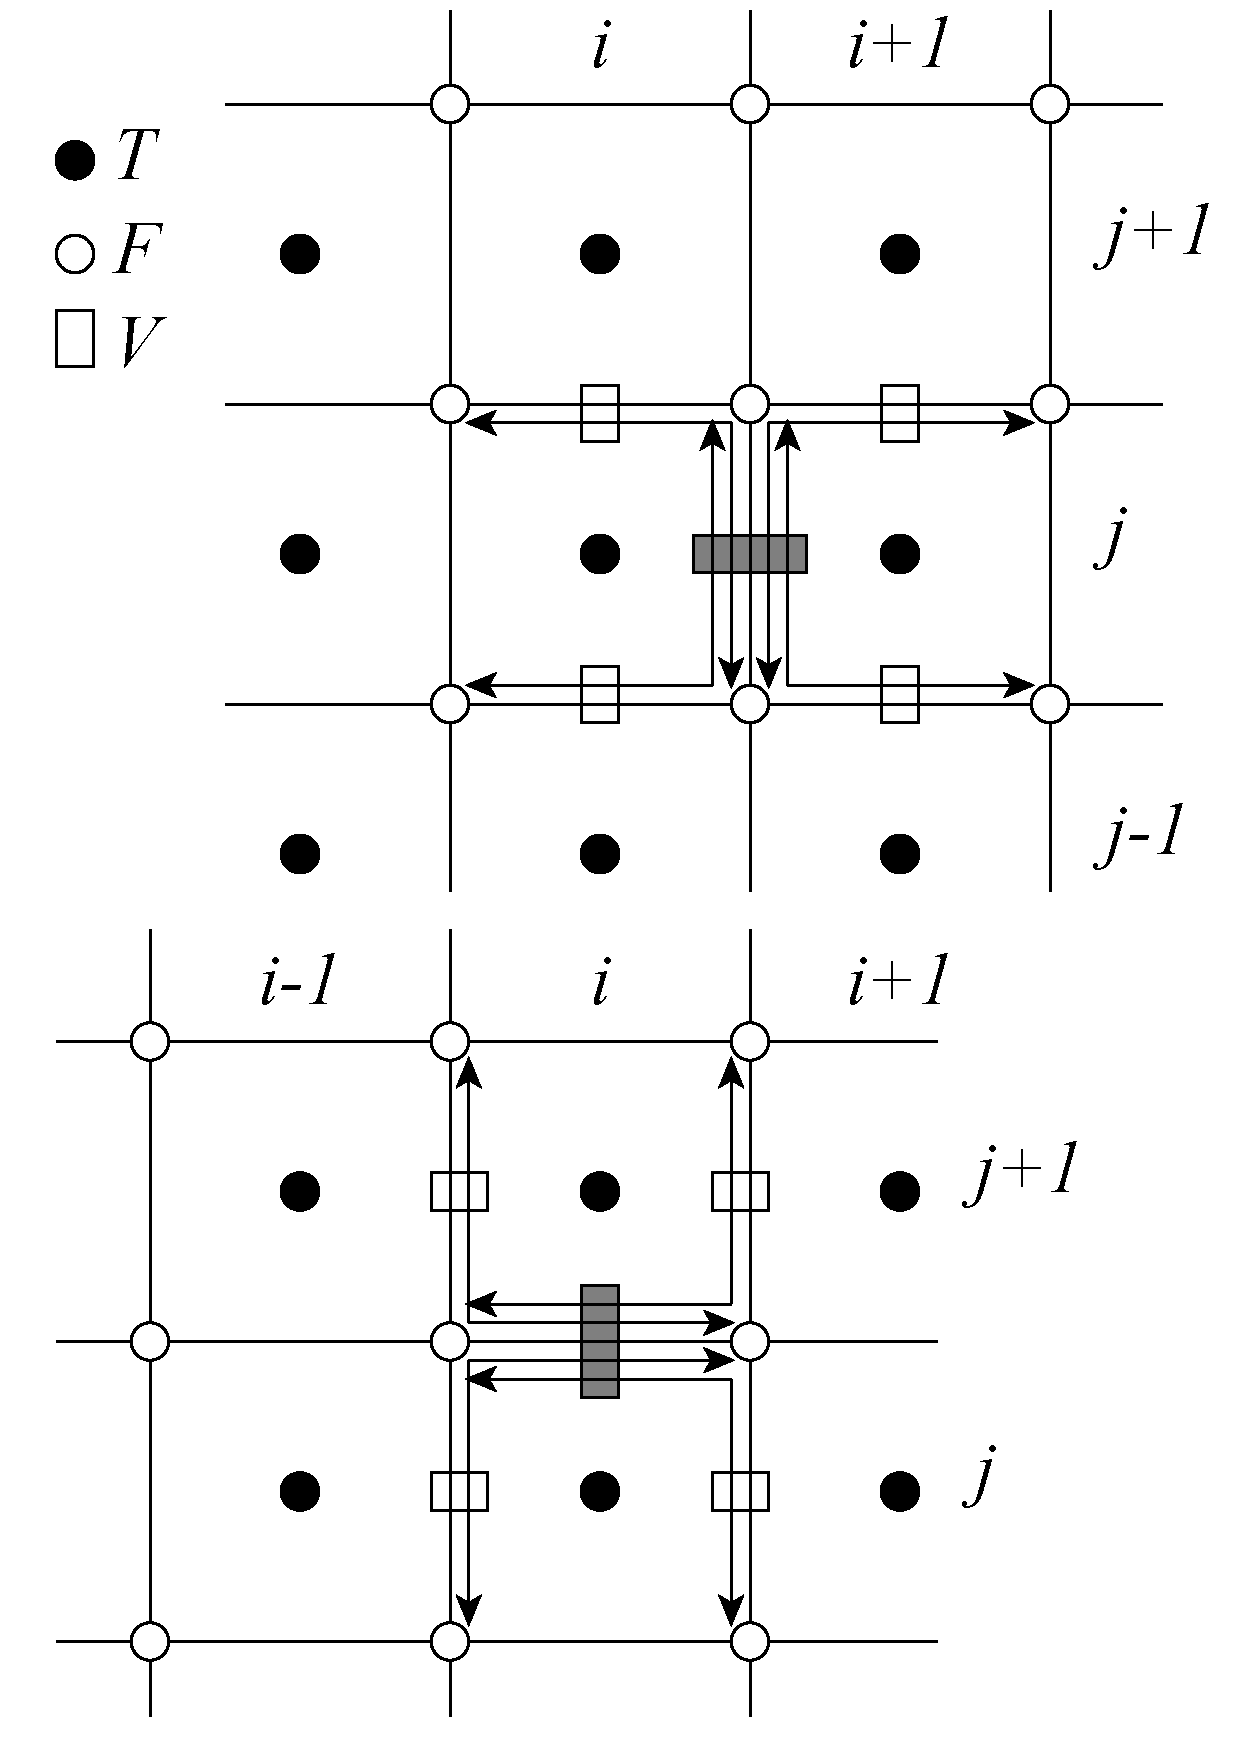
\includegraphics[width=0.70\textwidth]{./TexFiles/Figures/Fig_DYN_een_triad.pdf}
\caption{ \label{Fig_DYN_een_triad}  
Triads used in the energy and enstrophy conserving scheme (een) for 
$u$-component (upper panel) and $v$-component (lower panel).}
\end{center}   \end{figure}
%>>>>>>>>>>>>>>>>>>>>>>>>>>>>>>>>

Note that a key point in \eqref{Eq_een_e3f} is that the averaging in the \textbf{i}- and 
\textbf{j}- directions uses the masked vertical scale factor but is always divided by 
$4$, not by the sum of the masks at the four $T$-points. This preserves the continuity of 
$e_{3f}$ when one or more of the neighbouring $e_{3t}$ tends to zero and 
extends by continuity the value of $e_{3f}$ into the land areas. This feature is essential for 
the $z$-coordinate with partial steps.

Next, the vorticity triads, $ {^i_j}\mathbb{Q}^{i_p}_{j_p}$ can be defined at a $T$-point as 
the following triad combinations of the neighbouring potential vorticities defined at f-points 
(Fig.~\ref{Fig_DYN_een_triad}): 
\begin{equation} \label{Q_triads}
_i^j \mathbb{Q}^{i_p}_{j_p}
= \frac{1}{12} \ \left(   q^{i-i_p}_{j+j_p} + q^{i+j_p}_{j+i_p} + q^{i+i_p}_{j-j_p}  \right)
\end{equation}
where the indices $i_p$ and $k_p$ take the values: $i_p = -1/2$ or $1/2$ and $j_p = -1/2$ or $1/2$. 

Finally, the vorticity terms are represented as: 
\begin{equation} \label{Eq_dynvor_een}
\left\{ {
\begin{aligned}
 +q\,e_3 \, v 	&\equiv +\frac{1}{e_{1u} }   \sum_{\substack{i_p,\,k_p}} 
                         {^{i+1/2-i_p}_j}  \mathbb{Q}^{i_p}_{j_p}  \left( e_{1v}\,e_{3v} \;v  \right)^{i+1/2-i_p}_{j+j_p}   \\
 - q\,e_3 \, u     &\equiv -\frac{1}{e_{2v} }    \sum_{\substack{i_p,\,k_p}} 
                         {^i_{j+1/2-j_p}}  \mathbb{Q}^{i_p}_{j_p}  \left( e_{2u}\,e_{3u} \;u  \right)^{i+i_p}_{j+1/2-j_p}   \\
\end{aligned} 
} \right.
\end{equation} 

This EEN scheme in fact combines the conservation properties of the ENS and ENE schemes. 
It conserves both total energy and potential enstrophy in the limit of horizontally 
nondivergent flow ($i.e.$ $\chi$=$0$) (see  Appendix~\ref{Apdx_C_vorEEN}). 
Applied to a realistic ocean configuration, it has been shown that it leads to a significant 
reduction of the noise in the vertical velocity field \citep{Le_Sommer_al_OM09}. 
Furthermore, used in combination with a partial steps representation of bottom topography,
it improves the interaction between current and topography, leading to a larger
topostrophy of the flow  \citep{Barnier_al_OD06, Penduff_al_OS07}. 

%--------------------------------------------------------------------------------------------------------------
%           Kinetic Energy Gradient term
%--------------------------------------------------------------------------------------------------------------
\subsection   [Kinetic Energy Gradient term (\textit{dynkeg})]
			{Kinetic Energy Gradient term (\mdl{dynkeg})}
\label{DYN_keg}

As demonstrated in Appendix~\ref{Apdx_C}, there is a single discrete formulation 
of the kinetic energy gradient term that, together with the formulation chosen for 
the vertical advection (see below), conserves the total kinetic energy:
\begin{equation} \label{Eq_dynkeg}
\left\{ \begin{aligned}
 -\frac{1}{2 \; e_{1u} }  & \ \delta _{i+1/2} \left[ {\overline {u^2}^{\,i} + \overline{v^2}^{\,j}} \right]   \\
 -\frac{1}{2 \; e_{2v} }  & \ \delta _{j+1/2} \left[ {\overline {u^2}^{\,i} + \overline{v^2}^{\,j}} \right]    
\end{aligned} \right.
\end{equation} 

%--------------------------------------------------------------------------------------------------------------
%           Vertical advection term
%--------------------------------------------------------------------------------------------------------------
\subsection   [Vertical advection term (\textit{dynzad}) ]
			{Vertical advection term (\mdl{dynzad}) }
\label{DYN_zad}

The discrete formulation of the vertical advection, together with the formulation 
chosen for the gradient of kinetic energy (KE) term, conserves the total kinetic 
energy. Indeed, the change of KE due to the vertical advection is exactly 
balanced by the change of KE due to the gradient of KE (see Appendix~\ref{Apdx_C}).
\begin{equation} \label{Eq_dynzad}
\left\{ 		\begin{aligned}
-\frac{1} {e_{1u}\,e_{2u}\,e_{3u}} &\ \overline{\ \overline{ e_{1t}\,e_{2t}\;w } ^{\,i+1/2}  \;\delta _{k+1/2} \left[ u \right]\  }^{\,k}  \\
-\frac{1} {e_{1v}\,e_{2v}\,e_{3v}}  &\ \overline{\ \overline{ e_{1t}\,e_{2t}\;w } ^{\,j+1/2}  \;\delta _{k+1/2} \left[ u \right]\  }^{\,k} 
\end{aligned}         \right.
\end{equation} 

% ================================================================
% Coriolis and Advection : flux form
% ================================================================
\section{Coriolis and Advection: flux form}
\label{DYN_adv_cor_flux}
%------------------------------------------nam_dynadv----------------------------------------------------
\namdisplay{namdyn_adv} 
%-------------------------------------------------------------------------------------------------------------

Options are defined through the \ngn{namdyn\_adv} namelist variables.
In the flux form (as in the vector invariant form), the Coriolis and momentum 
advection terms are evaluated using a leapfrog scheme, $i.e.$ the velocity 
appearing in their expressions is centred in time (\textit{now} velocity). At the 
lateral boundaries either free slip, no slip or partial slip boundary conditions 
are applied following Chap.\ref{LBC}.


%--------------------------------------------------------------------------------------------------------------
%           Coriolis plus curvature metric terms
%--------------------------------------------------------------------------------------------------------------
\subsection   [Coriolis plus curvature metric terms (\textit{dynvor}) ]
			{Coriolis plus curvature metric terms (\mdl{dynvor}) }
\label{DYN_cor_flux}

In flux form, the vorticity term reduces to a Coriolis term in which the Coriolis 
parameter has been modified to account for the "metric" term. This altered 
Coriolis parameter is thus discretised at $f$-points. It is given by: 
\begin{multline} \label{Eq_dyncor_metric}
f+\frac{1}{e_1 e_2 }\left( {v\frac{\partial e_2 }{\partial i}  -  u\frac{\partial e_1 }{\partial j}} \right)  \\
   \equiv   f + \frac{1}{e_{1f} e_{2f} } \left( { \ \overline v ^{i+1/2}\delta _{i+1/2} \left[ {e_{2u} } \right]  
                                                                 -  \overline u ^{j+1/2}\delta _{j+1/2} \left[ {e_{1u} } \right]  }  \ \right)
\end{multline} 

Any of the (\ref{Eq_dynvor_ens}), (\ref{Eq_dynvor_ene}) and (\ref{Eq_dynvor_een}) 
schemes can be used to compute the product of the Coriolis parameter and the 
vorticity. However, the energy-conserving scheme  (\ref{Eq_dynvor_een}) has 
exclusively been used to date. This term is evaluated using a leapfrog scheme, 
$i.e.$ the velocity is centred in time (\textit{now} velocity).

%--------------------------------------------------------------------------------------------------------------
%           Flux form Advection term
%--------------------------------------------------------------------------------------------------------------
\subsection   [Flux form Advection term (\textit{dynadv}) ]
			{Flux form Advection term (\mdl{dynadv}) }
\label{DYN_adv_flux}

The discrete expression of the advection term is given by :
\begin{equation} \label{Eq_dynadv}
\left\{ 
\begin{aligned}
\frac{1}{e_{1u}\,e_{2u}\,e_{3u}} 
\left(      \delta _{i+1/2} \left[ \overline{e_{2u}\,e_{3u}\;u }^{i       }  \ u_t      \right]    
          + \delta _{j       } \left[ \overline{e_{1u}\,e_{3u}\;v }^{i+1/2}  \ u_f      \right] \right.  \ \;   \\
\left.   + \delta _{k      } \left[ \overline{e_{1w}\,e_{2w}\;w}^{i+1/2}  \ u_{uw} \right] \right)   \\
\\
\frac{1}{e_{1v}\,e_{2v}\,e_{3v}} 
\left(     \delta _{i       } \left[ \overline{e_{2u}\,e_{3u }\;u }^{j+1/2} \ v_f       \right] 
         + \delta _{j+1/2} \left[ \overline{e_{1u}\,e_{3u }\;v }^{i       } \ v_t       \right] \right.  \ \, \, \\
\left.  + \delta _{k      } \left[ \overline{e_{1w}\,e_{2w}\;w}^{j+1/2} \ v_{vw}  \right] \right) \\
\end{aligned}
\right.
\end{equation}

Two advection schemes are available: a $2^{nd}$ order centered finite 
difference scheme, CEN2, or a $3^{rd}$ order upstream biased scheme, UBS. 
The latter is described in \citet{Shchepetkin_McWilliams_OM05}. The schemes are 
selected using the namelist logicals \np{ln\_dynadv\_cen2} and \np{ln\_dynadv\_ubs}. 
In flux form, the schemes differ by the choice of a space and time interpolation to 
define the value of $u$ and $v$ at the centre of each face of $u$- and $v$-cells, 
$i.e.$ at the $T$-, $f$-, and $uw$-points for $u$ and at the $f$-, $T$- and 
$vw$-points for $v$. 

%-------------------------------------------------------------
%                 2nd order centred scheme
%-------------------------------------------------------------
\subsubsection{$2^{nd}$ order centred scheme (cen2) (\np{ln\_dynadv\_cen2}=true)}
\label{DYN_adv_cen2}

In the centered $2^{nd}$ order formulation, the velocity is evaluated as the 
mean of the two neighbouring points :
\begin{equation} \label{Eq_dynadv_cen2}
\left\{ 		\begin{aligned}
 u_T^{cen2} &=\overline u^{i }       \quad &  u_F^{cen2} &=\overline u^{j+1/2}  \quad &  u_{uw}^{cen2} &=\overline u^{k+1/2}   \\
 v_F^{cen2} &=\overline v ^{i+1/2} \quad & v_F^{cen2} &=\overline v^j		\quad &  v_{vw}^{cen2} &=\overline v ^{k+1/2}  \\
\end{aligned}      \right.
\end{equation} 

The scheme is non diffusive (i.e. conserves the kinetic energy) but dispersive 
($i.e.$ it may create false extrema). It is therefore notoriously noisy and must be 
used in conjunction with an explicit diffusion operator to produce a sensible solution. 
The associated time-stepping is performed using a leapfrog scheme in conjunction 
with an Asselin time-filter, so $u$ and $v$ are the \emph{now} velocities.

%-------------------------------------------------------------
%                 UBS scheme
%-------------------------------------------------------------
\subsubsection{Upstream Biased Scheme (UBS) (\np{ln\_dynadv\_ubs}=true)}
\label{DYN_adv_ubs}

The UBS advection scheme is an upstream biased third order scheme based on 
an upstream-biased parabolic interpolation. For example, the evaluation of 
$u_T^{ubs} $ is done as follows:
\begin{equation} \label{Eq_dynadv_ubs}
u_T^{ubs} =\overline u ^i-\;\frac{1}{6} 	\begin{cases}
		u"_{i-1/2}& 	\text{if $\ \overline{e_{2u}\,e_{3u} \ u}^i  \geqslant 0$ } 	\\
		u"_{i+1/2}& 	\text{if $\ \overline{e_{2u}\,e_{3u} \ u}^i  < 0$ }
\end{cases}
\end{equation}
where $u"_{i+1/2} =\delta _{i+1/2} \left[ {\delta _i \left[ u \right]} \right]$. This results 
in a dissipatively dominant ($i.e.$ hyper-diffusive) truncation error \citep{Shchepetkin_McWilliams_OM05}. 
The overall performance of the advection scheme is similar to that reported in 
\citet{Farrow1995}. It is a relatively good compromise between accuracy and 
smoothness. It is not a \emph{positive} scheme, meaning that false extrema are 
permitted. But the amplitudes of the false extrema are significantly reduced over 
those in the centred second order method. As the scheme already includes 
a diffusion component, it can be used without explicit  lateral diffusion on momentum 
($i.e.$ \np{ln\_dynldf\_lap}=\np{ln\_dynldf\_bilap}=false), and it is recommended to do so.

The UBS scheme is not used in all directions. In the vertical, the centred $2^{nd}$ 
order evaluation of the advection is preferred, $i.e.$ $u_{uw}^{ubs}$ and 
$u_{vw}^{ubs}$ in \eqref{Eq_dynadv_cen2} are used. UBS is diffusive and is 
associated with vertical mixing of momentum. \gmcomment{ gm  pursue the 
sentence:Since vertical mixing of momentum is a source term of the TKE equation...  }

For stability reasons,  the first term in (\ref{Eq_dynadv_ubs}), which corresponds 
to a second order centred scheme, is evaluated using the \textit{now} velocity 
(centred in time), while the second term, which is the diffusion part of the scheme, 
is evaluated using the \textit{before} velocity (forward in time). This is discussed 
by \citet{Webb_al_JAOT98} in the context of the Quick advection scheme.

Note that the UBS and QUICK (Quadratic Upstream Interpolation for Convective Kinematics) 
schemes only differ by one coefficient. Replacing $1/6$ by $1/8$ in 
(\ref{Eq_dynadv_ubs}) leads to the QUICK advection scheme \citep{Webb_al_JAOT98}. 
This option is not available through a namelist parameter, since the $1/6$ coefficient 
is hard coded. Nevertheless it is quite easy to make the substitution in the
\mdl{dynadv\_ubs} module and obtain a QUICK scheme.

Note also that in the current version of \mdl{dynadv\_ubs}, there is also the 
possibility of using a $4^{th}$ order evaluation of the advective velocity as in 
ROMS. This is an error and should be suppressed soon.
%%%
\gmcomment{action :  this have to be done}
%%%

% ================================================================
%           Hydrostatic pressure gradient term
% ================================================================
\section  [Hydrostatic pressure gradient (\textit{dynhpg})]
		{Hydrostatic pressure gradient (\mdl{dynhpg})}
\label{DYN_hpg}
%------------------------------------------nam_dynhpg---------------------------------------------------
\namdisplay{namdyn_hpg} 
%-------------------------------------------------------------------------------------------------------------

Options are defined through the \ngn{namdyn\_hpg} namelist variables.
The key distinction between the different algorithms used for the hydrostatic 
pressure gradient is the vertical coordinate used, since HPG is a \emph{horizontal} 
pressure gradient, $i.e.$ computed along geopotential surfaces. As a result, any 
tilt of the surface of the computational levels will require a specific treatment to 
compute the hydrostatic pressure gradient.

The hydrostatic pressure gradient term is evaluated either using a leapfrog scheme, 
$i.e.$ the density appearing in its expression is centred in time (\emph{now} $\rho$), or 
a semi-implcit scheme. At the lateral boundaries either free slip, no slip or partial slip 
boundary conditions are applied.

%--------------------------------------------------------------------------------------------------------------
%           z-coordinate with full step
%--------------------------------------------------------------------------------------------------------------
\subsection   [$z$-coordinate with full step (\np{ln\_dynhpg\_zco}) ]
			{$z$-coordinate with full step (\np{ln\_dynhpg\_zco}=true)}
\label{DYN_hpg_zco}

The hydrostatic pressure can be obtained by integrating the hydrostatic equation 
vertically from the surface. However, the pressure is large at great depth while its 
horizontal gradient is several orders of magnitude smaller. This may lead to large 
truncation errors in the pressure gradient terms. Thus, the two horizontal components 
of the hydrostatic pressure gradient are computed directly as follows:

for $k=km$ (surface layer, $jk=1$ in the code)
\begin{equation} \label{Eq_dynhpg_zco_surf}
\left\{ \begin{aligned}
					\left. \delta _{i+1/2} \left[  p^h 			 \right] \right|_{k=km} 
&= \frac{1}{2} g \ 	\left. \delta _{i+1/2} \left[  e_{3w} \ \rho \right] \right|_{k=km}   \\
     					\left. \delta _{j+1/2} \left[  p^h  			 \right] \right|_{k=km} 
&= \frac{1}{2} g \ 	\left. \delta _{j+1/2} \left[  e_{3w} \ \rho \right] \right|_{k=km}   \\
\end{aligned} \right.
\end{equation} 

for $1<k<km$ (interior layer)
\begin{equation} \label{Eq_dynhpg_zco}
\left\{ \begin{aligned}
					\left. \delta _{i+1/2} \left[  p^h 			 \right] \right|_{k} 
&=					\left. \delta _{i+1/2} \left[  p^h 			 \right] \right|_{k-1} 
+    \frac{1}{2}\;g\;	\left. \delta _{i+1/2} \left[  e_{3w} \ \overline {\rho}^{k+1/2} \right] \right|_{k}   \\
     					\left. \delta _{j+1/2} \left[  p^h  			 \right] \right|_{k} 
&=     				\left. \delta _{j+1/2} \left[  p^h  			 \right] \right|_{k-1} 
+    \frac{1}{2}\;g\;	\left. \delta _{j+1/2} \left[  e_{3w} \ \overline {\rho}^{k+1/2} \right] \right|_{k}   \\
\end{aligned} \right.
\end{equation} 

Note that the $1/2$ factor in (\ref{Eq_dynhpg_zco_surf}) is adequate because of 
the definition of $e_{3w}$ as the vertical derivative of the scale factor at the surface 
level ($z=0$). Note also that in case of variable volume level (\key{vvl} defined), the 
surface pressure gradient is included in \eqref{Eq_dynhpg_zco_surf} and \eqref{Eq_dynhpg_zco} 
through the space and time variations of the vertical scale factor $e_{3w}$.

%--------------------------------------------------------------------------------------------------------------
%           z-coordinate with partial step
%--------------------------------------------------------------------------------------------------------------
\subsection   [$z$-coordinate with partial step (\np{ln\_dynhpg\_zps})]
			{$z$-coordinate with partial step (\np{ln\_dynhpg\_zps}=true)}
\label{DYN_hpg_zps}

With partial bottom cells, tracers in horizontally adjacent cells generally live at 
different depths. Before taking horizontal gradients between these tracer points, 
a linear interpolation is used to approximate the deeper tracer as if it actually lived 
at the depth of the shallower tracer point. 

Apart from this modification, the horizontal hydrostatic pressure gradient evaluated 
in the $z$-coordinate with partial step is exactly as in the pure $z$-coordinate case. 
As explained in detail in section \S\ref{TRA_zpshde}, the nonlinearity of pressure 
effects in the equation of state is such that it is better to interpolate temperature and 
salinity vertically before computing the density. Horizontal gradients of temperature 
and salinity are needed for the TRA modules, which is the reason why the horizontal 
gradients of density at the deepest model level are computed in module \mdl{zpsdhe} 
located in the TRA directory and described in \S\ref{TRA_zpshde}.

%--------------------------------------------------------------------------------------------------------------
%           s- and s-z-coordinates
%--------------------------------------------------------------------------------------------------------------
\subsection{$s$- and $z$-$s$-coordinates}
\label{DYN_hpg_sco}

Pressure gradient formulations in an $s$-coordinate have been the subject of a vast 
number of papers ($e.g.$, \citet{Song1998, Shchepetkin_McWilliams_OM05}). 
A number of different pressure gradient options are coded but the ROMS-like, density Jacobian with 
cubic polynomial method is currently disabled whilst known bugs are under investigation.

$\bullet$ Traditional coding (see for example \citet{Madec_al_JPO96}: (\np{ln\_dynhpg\_sco}=true)
\begin{equation} \label{Eq_dynhpg_sco}
\left\{ \begin{aligned}
 - \frac{1}    					{\rho_o \, e_{1u}} \;	\delta _{i+1/2} \left[  p^h  \right] 
+ \frac{g\; \overline {\rho}^{i+1/2}}	{\rho_o \, e_{1u}} \;	\delta _{i+1/2} \left[  z_t   \right]    \\
 - \frac{1}    					{\rho_o \, e_{2v}} \;	\delta _{j+1/2} \left[  p^h  \right]  
+ \frac{g\; \overline {\rho}^{j+1/2}}	{\rho_o \, e_{2v}} \;	\delta _{j+1/2} \left[  z_t   \right]    \\
\end{aligned} \right.
\end{equation} 

Where the first term is the pressure gradient along coordinates, computed as in 
\eqref{Eq_dynhpg_zco_surf} - \eqref{Eq_dynhpg_zco}, and $z_T$ is the depth of 
the $T$-point evaluated from the sum of the vertical scale factors at the $w$-point 
($e_{3w}$).
 
$\bullet$ Traditional coding with adaptation for ice shelf cavities (\np{ln\_dynhpg\_isf}=true).
This scheme need the activation of ice shelf cavities (\np{ln\_isfcav}=true).

$\bullet$ Pressure Jacobian scheme (prj) (a research paper in preparation) (\np{ln\_dynhpg\_prj}=true)

$\bullet$ Density Jacobian with cubic polynomial scheme (DJC) \citep{Shchepetkin_McWilliams_OM05} 
(\np{ln\_dynhpg\_djc}=true) (currently disabled; under development)

Note that expression \eqref{Eq_dynhpg_sco} is commonly used when the variable volume formulation is
activated (\key{vvl}) because in that case, even with a flat bottom, the coordinate surfaces are not
horizontal but follow the free surface \citep{Levier2007}. The pressure jacobian scheme
(\np{ln\_dynhpg\_prj}=true) is available as an improved option to \np{ln\_dynhpg\_sco}=true when
\key{vvl} is active.  The pressure Jacobian scheme uses a constrained cubic spline to reconstruct
the density profile across the water column. This method maintains the monotonicity between the
density nodes  The pressure can be calculated by analytical integration of the density profile and a
pressure Jacobian method is used to solve the horizontal pressure gradient. This method can provide
a more accurate calculation of the horizontal pressure gradient than the standard scheme.

%--------------------------------------------------------------------------------------------------------------
%           Time-scheme
%--------------------------------------------------------------------------------------------------------------
\subsection   [Time-scheme (\np{ln\_dynhpg\_imp}) ]
			{Time-scheme (\np{ln\_dynhpg\_imp}= true/false)}
\label{DYN_hpg_imp}

The default time differencing scheme used for the horizontal pressure gradient is 
a leapfrog scheme and therefore the density used in all discrete expressions given 
above is the  \textit{now} density, computed from the \textit{now} temperature and 
salinity. In some specific cases (usually high resolution simulations over an ocean 
domain which includes weakly stratified regions) the physical phenomenon that 
controls the time-step is internal gravity waves (IGWs). A semi-implicit scheme for 
doubling the stability limit associated with IGWs can be used \citep{Brown_Campana_MWR78, 
Maltrud1998}. It involves the evaluation of the hydrostatic pressure gradient as an 
average over the three time levels $t-\rdt$, $t$, and $t+\rdt$ ($i.e.$  
\textit{before},  \textit{now} and  \textit{after} time-steps), rather than at the central 
time level $t$ only, as in the standard leapfrog scheme. 

$\bullet$ leapfrog scheme (\np{ln\_dynhpg\_imp}=true):

\begin{equation} \label{Eq_dynhpg_lf}
\frac{u^{t+\rdt}-u^{t-\rdt}}{2\rdt} = \;\cdots \;
	-\frac{1}{\rho _o \,e_{1u} }\delta _{i+1/2} \left[ {p_h^t } \right]
\end{equation}

$\bullet$ semi-implicit scheme (\np{ln\_dynhpg\_imp}=true):
\begin{equation} \label{Eq_dynhpg_imp}
\frac{u^{t+\rdt}-u^{t-\rdt}}{2\rdt} = \;\cdots \;
	-\frac{1}{4\,\rho _o \,e_{1u} } \delta_{i+1/2} \left[ p_h^{t+\rdt} +2\,p_h^t +p_h^{t-\rdt}  \right]
\end{equation}

The semi-implicit time scheme \eqref{Eq_dynhpg_imp} is made possible without 
significant additional computation since the density can be updated to time level 
$t+\rdt$ before computing the horizontal hydrostatic pressure gradient. It can 
be easily shown that the stability limit associated with the hydrostatic pressure 
gradient doubles using \eqref{Eq_dynhpg_imp} compared to that using the 
standard leapfrog scheme \eqref{Eq_dynhpg_lf}. Note that \eqref{Eq_dynhpg_imp} 
is equivalent to applying a time filter to the pressure gradient to eliminate high 
frequency IGWs. Obviously, when using \eqref{Eq_dynhpg_imp}, the doubling of 
the time-step is achievable only if no other factors control the time-step, such as 
the stability limits associated with advection or diffusion.

In practice, the semi-implicit scheme is used when \np{ln\_dynhpg\_imp}=true. 
In this case, we choose to apply the time filter to temperature and salinity used in 
the equation of state, instead of applying it to the hydrostatic pressure or to the 
density, so that no additional storage array has to be defined. The density used to 
compute the hydrostatic pressure gradient (whatever the formulation) is evaluated 
as follows:
\begin{equation} \label{Eq_rho_flt}
	\rho^t = \rho( \widetilde{T},\widetilde {S},z_t)
 \quad	  \text{with}	\quad 
	\widetilde{X} = 1 / 4 \left(  X^{t+\rdt} +2 \,X^t + X^{t-\rdt}  \right)
\end{equation}

Note that in the semi-implicit case, it is necessary to save the filtered density, an 
extra three-dimensional field, in the restart file to restart the model with exact 
reproducibility. This option is controlled by  \np{nn\_dynhpg\_rst}, a namelist parameter.

% ================================================================
% Surface Pressure Gradient
% ================================================================
\section  [Surface pressure gradient (\textit{dynspg}) ]
		{Surface pressure gradient (\mdl{dynspg})}
\label{DYN_spg}
%-----------------------------------------nam_dynspg----------------------------------------------------
\namdisplay{namdyn_spg} 
%------------------------------------------------------------------------------------------------------------

$\ $\newline      %force an empty line

%%%
Options are defined through the \ngn{namdyn\_spg} namelist variables.
The surface pressure gradient term is related to the representation of the free surface (\S\ref{PE_hor_pg}). The main distinction is between the fixed volume case (linear free surface) and the variable volume case (nonlinear free surface, \key{vvl} is defined). In the linear free surface case (\S\ref{PE_free_surface}) the vertical scale factors $e_{3}$ are fixed in time, while they are time-dependent in the nonlinear case (\S\ref{PE_free_surface}). With both linear and nonlinear free surface, external gravity waves are allowed in the equations, which imposes a very small time step when an explicit time stepping is used. Two methods are proposed to allow a longer time step for the three-dimensional equations: the filtered free surface, which is a modification of the continuous equations (see \eqref{Eq_PE_flt}), and the split-explicit free surface described below. The extra term introduced in the filtered method is calculated implicitly, so that the update of the next velocities is done in module \mdl{dynspg\_flt} and not in \mdl{dynnxt}.

%%%


The form of the surface pressure gradient term depends on how the user wants to handle 
the fast external gravity waves that are a solution of the analytical equation (\S\ref{PE_hor_pg}). 
Three formulations are available, all controlled by a CPP key (ln\_dynspg\_xxx):
an explicit formulation which requires a small time step ;
a filtered free surface formulation which allows a larger time step by adding a filtering 
term into the momentum equation ; 
and a split-explicit free surface formulation, described below, which also allows a larger time step.

The extra term introduced in the filtered method is calculated 
implicitly, so that a solver is used to compute it. As a consequence the update of the $next$ 
velocities is done in module \mdl{dynspg\_flt} and not in \mdl{dynnxt}.



%--------------------------------------------------------------------------------------------------------------
% Explicit free surface formulation
%--------------------------------------------------------------------------------------------------------------
\subsection{Explicit free surface (\key{dynspg\_exp})}
\label{DYN_spg_exp}

In the explicit free surface formulation (\key{dynspg\_exp} defined), the model time step 
is chosen to be small enough to resolve the external gravity waves (typically a few tens of seconds). 
The surface pressure gradient, evaluated using a leap-frog scheme ($i.e.$ centered in time),
is thus simply given by :
\begin{equation} \label{Eq_dynspg_exp}
\left\{ \begin{aligned}
 - \frac{1}{e_{1u}\,\rho_o} \;	\delta _{i+1/2} \left[  \,\rho \,\eta\,  \right] 	\\
 - \frac{1}{e_{2v}\,\rho_o} \;	\delta _{j+1/2} \left[  \,\rho \,\eta\,  \right]  
\end{aligned} \right.
\end{equation} 

Note that in the non-linear free surface case ($i.e.$ \key{vvl} defined), the surface pressure 
gradient is already included in the momentum tendency  through the level thickness variation 
allowed in the computation of the hydrostatic pressure gradient. Thus, nothing is done in the \mdl{dynspg\_exp} module.

%--------------------------------------------------------------------------------------------------------------
% Split-explict free surface formulation
%--------------------------------------------------------------------------------------------------------------
\subsection{Split-Explicit free surface (\key{dynspg\_ts})}
\label{DYN_spg_ts}
%------------------------------------------namsplit-----------------------------------------------------------
\namdisplay{namsplit} 
%-------------------------------------------------------------------------------------------------------------

The split-explicit free surface formulation used in \NEMO (\key{dynspg\_ts} defined),
also called the time-splitting formulation, follows the one 
proposed by \citet{Shchepetkin_McWilliams_OM05}. The general idea is to solve the free surface 
equation and the associated barotropic velocity equations with a smaller time 
step than $\rdt$, the time step used for the three dimensional prognostic 
variables (Fig.~\ref{Fig_DYN_dynspg_ts}). 
The size of the small time step, $\rdt_e$ (the external mode or barotropic time step)
 is provided through the \np{nn\_baro} namelist parameter as: 
$\rdt_e = \rdt / nn\_baro$. This parameter can be optionally defined automatically (\np{ln\_bt\_nn\_auto}=true) 
considering that the stability of the barotropic system is essentially controled by external waves propagation. 
Maximum allowed Courant number is in that case time independent, and easily computed online from the input bathymetry.

%%%
The barotropic mode solves the following equations:
\begin{subequations} \label{Eq_BT}
  \begin{equation}     \label{Eq_BT_dyn}
\frac{\partial {\rm \overline{{\bf U}}_h} }{\partial t}=
 -f\;{\rm {\bf k}}\times {\rm \overline{{\bf U}}_h} 
-g\nabla _h \eta -\frac{c_b^{\textbf U}}{H+\eta} \rm {\overline{{\bf U}}_h} + \rm {\overline{\bf G}}
  \end{equation}

  \begin{equation} \label{Eq_BT_ssh}
\frac{\partial \eta }{\partial t}=-\nabla \cdot \left[ {\left( {H+\eta } \right) \; {\rm{\bf \overline{U}}}_h \,} \right]+P-E
  \end{equation}
\end{subequations}
where $\rm {\overline{\bf G}}$ is a forcing term held constant, containing coupling term between modes, surface atmospheric forcing as well as slowly varying barotropic terms not explicitly computed to gain efficiency. The third term on the right hand side of \eqref{Eq_BT_dyn} represents the bottom stress (see section \S\ref{ZDF_bfr}), explicitly accounted for at each barotropic iteration. Temporal discretization of the system above follows a three-time step Generalized Forward Backward algorithm detailed in \citet{Shchepetkin_McWilliams_OM05}. AB3-AM4 coefficients used in \NEMO follow the second-order accurate, "multi-purpose" stability compromise as defined in \citet{Shchepetkin_McWilliams_Bk08} (see their figure 12, lower left). 

%>   >   >   >   >   >   >   >   >   >   >   >   >   >   >   >   >   >   >   >   >   >   >   >   >   >   >   >
\begin{figure}[!t]    \begin{center}
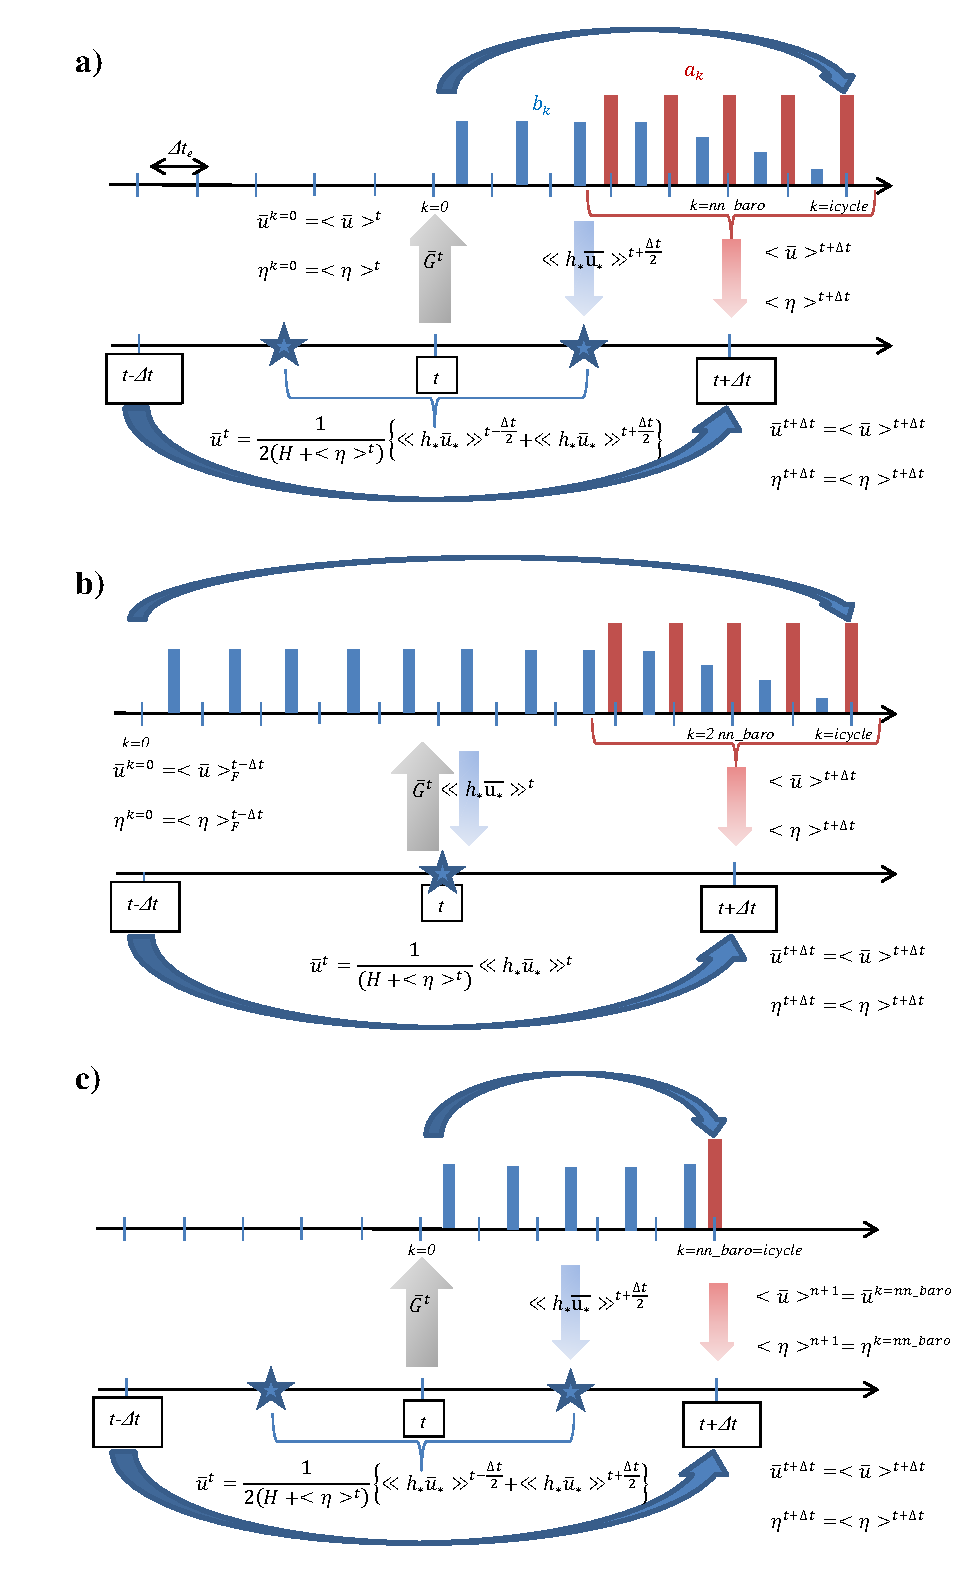
\includegraphics[width=0.7\textwidth]{./TexFiles/Figures/Fig_DYN_dynspg_ts.pdf}
\caption{  \label{Fig_DYN_dynspg_ts}
Schematic of the split-explicit time stepping scheme for the external 
and internal modes. Time increases to the right. In this particular exemple, 
a boxcar averaging window over $nn\_baro$ barotropic time steps is used ($nn\_bt\_filt=1$) and $nn\_baro=5$.
Internal mode time steps (which are also the model time steps) are denoted 
by $t-\rdt$, $t$ and $t+\rdt$. Variables with $k$ superscript refer to instantaneous barotropic variables, 
$< >$ and $<< >>$ operator refer to time filtered variables using respectively primary (red vertical bars) and secondary weights (blue vertical bars). 
The former are used to obtain time filtered quantities at $t+\rdt$ while the latter are used to obtain time averaged 
transports to advect tracers.
a) Forward time integration: \np{ln\_bt\_fw}=true, \np{ln\_bt\_ave}=true. 
b) Centred time integration: \np{ln\_bt\_fw}=false, \np{ln\_bt\_ave}=true. 
c) Forward time integration with no time filtering (POM-like scheme): \np{ln\_bt\_fw}=true, \np{ln\_bt\_ave}=false. }
\end{center}    \end{figure}
%>   >   >   >   >   >   >   >   >   >   >   >   >   >   >   >   >   >   >   >   >   >   >   >   >   >   >   >

In the default case (\np{ln\_bt\_fw}=true), the external mode is integrated 
between \textit{now} and  \textit{after} baroclinic time-steps (Fig.~\ref{Fig_DYN_dynspg_ts}a). To avoid aliasing of fast barotropic motions into three dimensional equations, time filtering is eventually applied on barotropic 
quantities (\np{ln\_bt\_ave}=true). In that case, the integration is extended slightly beyond  \textit{after} time step to provide time filtered quantities. 
These are used for the subsequent initialization of the barotropic mode in the following baroclinic step. 
Since external mode equations written at baroclinic time steps finally follow a forward time stepping scheme, 
asselin filtering is not applied to barotropic quantities. \\
Alternatively, one can choose to integrate barotropic equations starting 
from \textit{before} time step (\np{ln\_bt\_fw}=false). Although more computationaly expensive ( \np{nn\_baro} additional iterations are indeed necessary), the baroclinic to barotropic forcing term given at \textit{now} time step 
become centred in the middle of the integration window. It can easily be shown that this property 
removes part of splitting errors between modes, which increases the overall numerical robustness.
%references to Patrick Marsaleix' work here. Also work done by SHOM group.

%%%

As far as tracer conservation is concerned, barotropic velocities used to advect tracers must also be updated 
at \textit{now} time step. This implies to change the traditional order of computations in \NEMO: most of momentum  
trends (including the barotropic mode calculation) updated first, tracers' after. This \textit{de facto} makes semi-implicit hydrostatic 
pressure gradient (see section \S\ref{DYN_hpg_imp}) and time splitting not compatible. 
Advective barotropic velocities are obtained by using a secondary set of filtering weights, uniquely defined from the filter 
coefficients used for the time averaging (\citet{Shchepetkin_McWilliams_OM05}). Consistency between the time averaged continuity equation and the time stepping of tracers is here the key to obtain exact conservation.

%%%

One can eventually choose to feedback instantaneous values by not using any time filter (\np{ln\_bt\_ave}=false). 
In that case, external mode equations are continuous in time, ie they are not re-initialized when starting a new 
sub-stepping sequence. This is the method used so far in the POM model, the stability being maintained by refreshing at (almost) 
each barotropic time step advection and horizontal diffusion terms. Since the latter terms have not been added in \NEMO for 
computational efficiency, removing time filtering is not recommended except for debugging purposes. 
This may be used for instance to appreciate the damping effect of the standard formulation on external gravity waves in idealized or weakly non-linear cases. Although the damping is lower than for the filtered free surface, it is still significant as shown by \citet{Levier2007} in the case of an analytical barotropic Kelvin wave.

%>>>>>===============
\gmcomment{               %%% copy from griffies Book 

\textbf{title: Time stepping the barotropic system }

Assume knowledge of the full velocity and tracer fields at baroclinic time $\tau$. Hence, 
we can update the surface height and vertically integrated velocity with a leap-frog 
scheme using the small barotropic time step $\rdt$. We have 

\begin{equation} \label{DYN_spg_ts_eta}
\eta^{(b)}(\tau,t_{n+1}) - \eta^{(b)}(\tau,t_{n+1}) (\tau,t_{n-1})
	= 2 \rdt \left[-\nabla \cdot \textbf{U}^{(b)}(\tau,t_n) + \text{EMP}_w(\tau) \right] 
\end{equation}
\begin{multline} \label{DYN_spg_ts_u}
\textbf{U}^{(b)}(\tau,t_{n+1}) - \textbf{U}^{(b)}(\tau,t_{n-1})  \\
	= 2\rdt \left[ - f \textbf{k} \times \textbf{U}^{(b)}(\tau,t_{n}) 
	- H(\tau) \nabla p_s^{(b)}(\tau,t_{n}) +\textbf{M}(\tau) \right]
\end{multline}
\

In these equations, araised (b) denotes values of surface height and vertically integrated velocity updated with the barotropic time steps. The $\tau$ time label on $\eta^{(b)}$ 
and $U^{(b)}$ denotes the baroclinic time at which the vertically integrated forcing $\textbf{M}(\tau)$ (note that this forcing includes the surface freshwater forcing), the tracer fields, the freshwater flux $\text{EMP}_w(\tau)$, and total depth of the ocean $H(\tau)$ are held for the duration of the barotropic time stepping over a single cycle. This is also the time 
that sets the barotropic time steps via 
\begin{equation} \label{DYN_spg_ts_t}
t_n=\tau+n\rdt   
\end{equation}
with $n$ an integer. The density scaled surface pressure is evaluated via 
\begin{equation} \label{DYN_spg_ts_ps}
p_s^{(b)}(\tau,t_{n}) = \begin{cases}
	g \;\eta_s^{(b)}(\tau,t_{n}) \;\rho(\tau)_{k=1}) / \rho_o  &      \text{non-linear case} \\
	g \;\eta_s^{(b)}(\tau,t_{n})  &      \text{linear case} 
	\end{cases}
\end{equation}
To get started, we assume the following initial conditions 
\begin{equation} \label{DYN_spg_ts_eta}
\begin{split}
\eta^{(b)}(\tau,t_{n=0}) &= \overline{\eta^{(b)}(\tau)}
\\
\eta^{(b)}(\tau,t_{n=1}) &= \eta^{(b)}(\tau,t_{n=0}) + \rdt \ \text{RHS}_{n=0} 
\end{split}
\end{equation}
with 
\begin{equation} \label{DYN_spg_ts_etaF}
 \overline{\eta^{(b)}(\tau)} = \frac{1}{N+1} \sum\limits_{n=0}^N \eta^{(b)}(\tau-\rdt,t_{n})
\end{equation}
the time averaged surface height taken from the previous barotropic cycle. Likewise, 
\begin{equation} \label{DYN_spg_ts_u}
\textbf{U}^{(b)}(\tau,t_{n=0}) = \overline{\textbf{U}^{(b)}(\tau)}	\\
\\
\textbf{U}(\tau,t_{n=1}) = \textbf{U}^{(b)}(\tau,t_{n=0}) + \rdt \ \text{RHS}_{n=0}  	
\end{equation}
with 
\begin{equation} \label{DYN_spg_ts_u}
 \overline{\textbf{U}^{(b)}(\tau)} 
 	= \frac{1}{N+1} \sum\limits_{n=0}^N\textbf{U}^{(b)}(\tau-\rdt,t_{n})
\end{equation}
the time averaged vertically integrated transport. Notably, there is no Robert-Asselin time filter used in the barotropic portion of the integration. 

Upon reaching $t_{n=N} = \tau + 2\rdt \tau$ , the vertically integrated velocity is time averaged to produce the updated vertically integrated velocity at baroclinic time $\tau + \rdt \tau$ 
\begin{equation} \label{DYN_spg_ts_u}
\textbf{U}(\tau+\rdt) = \overline{\textbf{U}^{(b)}(\tau+\rdt)} 
 	= \frac{1}{N+1} \sum\limits_{n=0}^N\textbf{U}^{(b)}(\tau,t_{n})
\end{equation}
The surface height on the new baroclinic time step is then determined via a baroclinic leap-frog using the following form 

\begin{equation} \label{DYN_spg_ts_ssh}
\eta(\tau+\Delta) - \eta^{F}(\tau-\Delta) = 2\rdt \ \left[ - \nabla \cdot \textbf{U}(\tau) + \text{EMP}_w \right]  
\end{equation}

 The use of this "big-leap-frog" scheme for the surface height ensures compatibility between the mass/volume budgets and the tracer budgets. More discussion of this point is provided in Chapter 10 (see in particular Section 10.2). 
 
In general, some form of time filter is needed to maintain integrity of the surface 
height field due to the leap-frog splitting mode in equation \ref{DYN_spg_ts_ssh}. We 
have tried various forms of such filtering, with the following method discussed in 
\cite{Griffies_al_MWR01} chosen due to its stability and reasonably good maintenance of 
tracer conservation properties (see Section ??) 

\begin{equation} \label{DYN_spg_ts_sshf}
\eta^{F}(\tau-\Delta) =  \overline{\eta^{(b)}(\tau)} 
\end{equation}
Another approach tried was 

\begin{equation} \label{DYN_spg_ts_sshf2}
\eta^{F}(\tau-\Delta) = \eta(\tau) 
	+ (\alpha/2) \left[\overline{\eta^{(b)}}(\tau+\rdt)
				    + \overline{\eta^{(b)}}(\tau-\rdt) -2 \;\eta(\tau) \right]
\end{equation}

which is useful since it isolates all the time filtering aspects into the term multiplied 
by $\alpha$. This isolation allows for an easy check that tracer conservation is exact when 
eliminating tracer and surface height time filtering (see Section ?? for more complete discussion). However, in the general case with a non-zero $\alpha$, the filter \ref{DYN_spg_ts_sshf} was found to be more conservative, and so is recommended. 

}            %%end gm comment (copy of griffies book)

%>>>>>===============


%--------------------------------------------------------------------------------------------------------------
% Filtered free surface formulation
%--------------------------------------------------------------------------------------------------------------
\subsection{Filtered free surface (\key{dynspg\_flt})}
\label{DYN_spg_fltp}

The filtered formulation follows the \citet{Roullet_Madec_JGR00} implementation. 
The extra term introduced in the equations (see \S\ref{PE_free_surface}) is solved implicitly. 
The elliptic solvers available in the code are documented in \S\ref{MISC}.

%% gm %%======>>>>   given here the discrete eqs provided to the solver
\gmcomment{               %%% copy from chap-model basics 
\begin{equation} \label{Eq_spg_flt}
\frac{\partial {\rm {\bf U}}_h }{\partial t}= {\rm {\bf M}}
- g \nabla \left( \tilde{\rho} \ \eta \right) 
- g \ T_c \nabla \left( \widetilde{\rho} \ \partial_t \eta \right) 
\end{equation}
where $T_c$, is a parameter with dimensions of time which characterizes the force, 
$\widetilde{\rho} = \rho / \rho_o$ is the dimensionless density, and $\rm {\bf M}$ 
represents the collected contributions of the Coriolis, hydrostatic pressure gradient, 
non-linear and viscous terms in \eqref{Eq_PE_dyn}.
}   %end gmcomment

Note that in the linear free surface formulation (\key{vvl} not defined), the ocean depth 
is time-independent and so is the matrix to be inverted. It is computed once and for all and applies to all ocean time steps. 

% ================================================================
% Lateral diffusion term
% ================================================================
\section  [Lateral diffusion term (\textit{dynldf})]
		{Lateral diffusion term (\mdl{dynldf})}
\label{DYN_ldf}
%------------------------------------------nam_dynldf----------------------------------------------------
\namdisplay{namdyn_ldf} 
%-------------------------------------------------------------------------------------------------------------

Options are defined through the \ngn{namdyn\_ldf} namelist variables.
The options available for lateral diffusion are to use either laplacian 
(rotated or not) or biharmonic operators. The coefficients may be constant 
or spatially variable; the description of the coefficients is found in the chapter 
on lateral physics (Chap.\ref{LDF}). The lateral diffusion of momentum is 
evaluated using a forward scheme, $i.e.$ the velocity appearing in its expression 
is the \textit{before} velocity in time, except for the pure vertical component 
that appears when a tensor of rotation is used. This latter term is solved 
implicitly together with the vertical diffusion term (see \S\ref{STP}) 

At the lateral boundaries either free slip, no slip or partial slip boundary 
conditions are applied according to the user's choice (see Chap.\ref{LBC}).

% ================================================================
\subsection   [Iso-level laplacian operator (\np{ln\_dynldf\_lap}) ]
			{Iso-level laplacian operator (\np{ln\_dynldf\_lap}=true)}
\label{DYN_ldf_lap}

For lateral iso-level diffusion, the discrete operator is: 
\begin{equation} \label{Eq_dynldf_lap}
\left\{ \begin{aligned}
 D_u^{l{\rm {\bf U}}} =\frac{1}{e_{1u} }\delta _{i+1/2} \left[ {A_T^{lm} 
\;\chi } \right]-\frac{1}{e_{2u} {\kern 1pt}e_{3u} }\delta _j \left[ 
{A_f^{lm} \;e_{3f} \zeta } \right] \\ 
\\
 D_v^{l{\rm {\bf U}}} =\frac{1}{e_{2v} }\delta _{j+1/2} \left[ {A_T^{lm} 
\;\chi } \right]+\frac{1}{e_{1v} {\kern 1pt}e_{3v} }\delta _i \left[ 
{A_f^{lm} \;e_{3f} \zeta } \right] \\ 
\end{aligned} \right.
\end{equation} 

As explained in \S\ref{PE_ldf}, this formulation (as the gradient of a divergence 
and curl of the vorticity) preserves symmetry and ensures a complete 
separation between the vorticity and divergence parts of the momentum diffusion. 

%--------------------------------------------------------------------------------------------------------------
%           Rotated laplacian operator
%--------------------------------------------------------------------------------------------------------------
\subsection   [Rotated laplacian operator (\np{ln\_dynldf\_iso}) ]
			{Rotated laplacian operator (\np{ln\_dynldf\_iso}=true)}
\label{DYN_ldf_iso}

A rotation of the lateral momentum diffusion operator is needed in several cases: 
for iso-neutral diffusion in the $z$-coordinate (\np{ln\_dynldf\_iso}=true) and for 
either iso-neutral (\np{ln\_dynldf\_iso}=true) or geopotential 
(\np{ln\_dynldf\_hor}=true) diffusion in the $s$-coordinate. In the partial step 
case, coordinates are horizontal except at the deepest level and no 
rotation is performed when \np{ln\_dynldf\_hor}=true. The diffusion operator 
is defined simply as the divergence of down gradient momentum fluxes on each 
momentum component. It must be emphasized that this formulation ignores 
constraints on the stress tensor such as symmetry. The resulting discrete 
representation is:
\begin{equation} \label{Eq_dyn_ldf_iso}
\begin{split}
 D_u^{l\textbf{U}} &= \frac{1}{e_{1u} \, e_{2u} \, e_{3u} }	\\
&  \left\{\quad  {\delta _{i+1/2} \left[ {A_T^{lm}  \left( 
	 {\frac{e_{2t} \; e_{3t} }{e_{1t} } \,\delta _{i}[u]
	-e_{2t} \; r_{1t} \,\overline{\overline {\delta _{k+1/2}[u]}}^{\,i,\,k}}
 \right)} \right]} 	\right.
\\ 
& \qquad +\ \delta_j \left[ {A_f^{lm} \left( {\frac{e_{1f}\,e_{3f} }{e_{2f} 
}\,\delta _{j+1/2} [u] - e_{1f}\, r_{2f} 
\,\overline{\overline {\delta _{k+1/2} [u]}} ^{\,j+1/2,\,k}} 
\right)} \right] 
\\ 
&\qquad +\ \delta_k \left[ {A_{uw}^{lm} \left( {-e_{2u} \, r_{1uw} \,\overline{\overline 
{\delta_{i+1/2} [u]}}^{\,i+1/2,\,k+1/2} } 
\right.} \right. 
\\ 
&  \ \qquad \qquad \qquad \quad\ 
- e_{1u} \, r_{2uw} \,\overline{\overline {\delta_{j+1/2} [u]}} ^{\,j,\,k+1/2}
\\ 
& \left. {\left. { \ \qquad \qquad \qquad \ \ \ \left. {\ 
+\frac{e_{1u}\, e_{2u} }{e_{3uw} }\,\left( {r_{1uw}^2+r_{2uw}^2} 
\right)\,\delta_{k+1/2} [u]} \right)} \right]\;\;\;} \right\} 
\\
\\
 D_v^{l\textbf{V}} &= \frac{1}{e_{1v} \, e_{2v} \, e_{3v} }    \\
&  \left\{\quad  {\delta _{i+1/2} \left[ {A_f^{lm}  \left( 
	 {\frac{e_{2f} \; e_{3f} }{e_{1f} } \,\delta _{i+1/2}[v]
	-e_{2f} \; r_{1f} \,\overline{\overline {\delta _{k+1/2}[v]}}^{\,i+1/2,\,k}}
 \right)} \right]} 	\right.
\\ 
& \qquad +\ \delta_j \left[ {A_T^{lm} \left( {\frac{e_{1t}\,e_{3t} }{e_{2t} 
}\,\delta _{j} [v] - e_{1t}\, r_{2t} 
\,\overline{\overline {\delta _{k+1/2} [v]}} ^{\,j,\,k}} 
\right)} \right] 
\\ 
& \qquad +\ \delta_k \left[ {A_{vw}^{lm} \left( {-e_{2v} \, r_{1vw} \,\overline{\overline 
{\delta_{i+1/2} [v]}}^{\,i+1/2,\,k+1/2} }\right.} \right. 
\\
&  \ \qquad \qquad \qquad \quad\ 
- e_{1v} \, r_{2vw} \,\overline{\overline {\delta_{j+1/2} [v]}} ^{\,j+1/2,\,k+1/2}
\\ 
& \left. {\left. { \ \qquad \qquad \qquad \ \ \ \left. {\ 
+\frac{e_{1v}\, e_{2v} }{e_{3vw} }\,\left( {r_{1vw}^2+r_{2vw}^2} 
\right)\,\delta_{k+1/2} [v]} \right)} \right]\;\;\;} \right\} 
 \end{split}
\end{equation}
where $r_1$ and $r_2$ are the slopes between the surface along which the 
diffusion operator acts and the surface of computation ($z$- or $s$-surfaces). 
The way these slopes are evaluated is given in the lateral physics chapter 
(Chap.\ref{LDF}).

%--------------------------------------------------------------------------------------------------------------
%           Iso-level bilaplacian operator
%--------------------------------------------------------------------------------------------------------------
\subsection   [Iso-level bilaplacian operator (\np{ln\_dynldf\_bilap})]
			{Iso-level bilaplacian operator (\np{ln\_dynldf\_bilap}=true)}
\label{DYN_ldf_bilap}

The lateral fourth order operator formulation on momentum is obtained by 
applying \eqref{Eq_dynldf_lap} twice. It requires an additional assumption on 
boundary conditions: the first derivative term normal to the coast depends on 
the free or no-slip lateral boundary conditions chosen, while the third 
derivative terms normal to the coast are set to zero (see Chap.\ref{LBC}).
%%%
\gmcomment{add a remark on the the change in the position of the coefficient}
%%%

% ================================================================
%           Vertical diffusion term
% ================================================================
\section  [Vertical diffusion term (\mdl{dynzdf})]
		{Vertical diffusion term (\mdl{dynzdf})}
\label{DYN_zdf}
%----------------------------------------------namzdf------------------------------------------------------
\namdisplay{namzdf} 
%-------------------------------------------------------------------------------------------------------------

Options are defined through the \ngn{namzdf} namelist variables.
The large vertical diffusion coefficient found in the surface mixed layer together 
with high vertical resolution implies that in the case of explicit time stepping there 
would be too restrictive a constraint on the time step. Two time stepping schemes 
can be used for the vertical diffusion term : $(a)$ a forward time differencing 
scheme (\np{ln\_zdfexp}=true) using a time splitting technique 
(\np{nn\_zdfexp} $>$ 1) or $(b)$ a backward (or implicit) time differencing scheme 
(\np{ln\_zdfexp}=false) (see \S\ref{STP}). Note that namelist variables 
\np{ln\_zdfexp} and \np{nn\_zdfexp} apply to both tracers and dynamics. 

The formulation of the vertical subgrid scale physics is the same whatever 
the vertical coordinate is. The vertical diffusion operators given by 
\eqref{Eq_PE_zdf} take the following semi-discrete space form:
\begin{equation} \label{Eq_dynzdf}
\left\{   \begin{aligned}
D_u^{vm} &\equiv \frac{1}{e_{3u}} \ \delta _k \left[ \frac{A_{uw}^{vm} }{e_{3uw} }
                              \ \delta _{k+1/2} [\,u\,]         \right]     \\
\\
D_v^{vm} &\equiv \frac{1}{e_{3v}} \ \delta _k \left[ \frac{A_{vw}^{vm} }{e_{3vw} }
                              \ \delta _{k+1/2} [\,v\,]         \right]
\end{aligned}   \right.
\end{equation} 
where $A_{uw}^{vm} $ and $A_{vw}^{vm} $ are the vertical eddy viscosity and 
diffusivity coefficients. The way these coefficients are evaluated 
depends on the vertical physics used (see \S\ref{ZDF}).

The surface boundary condition on momentum is the stress exerted by 
the wind. At the surface, the momentum fluxes are prescribed as the boundary 
condition on the vertical turbulent momentum fluxes,
\begin{equation} \label{Eq_dynzdf_sbc}
\left.{\left( {\frac{A^{vm} }{e_3 }\ \frac{\partial \textbf{U}_h}{\partial k}} \right)} \right|_{z=1}
	 = \frac{1}{\rho _o} \binom{\tau _u}{\tau _v }
\end{equation}
where $\left( \tau _u ,\tau _v \right)$ are the two components of the wind stress 
vector in the (\textbf{i},\textbf{j}) coordinate system. The high mixing coefficients 
in the surface mixed layer ensure that the surface wind stress is distributed in 
the vertical over the mixed layer depth. If the vertical mixing coefficient 
is small (when no mixed layer scheme is used) the surface stress enters only 
the top model level, as a body force. The surface wind stress is calculated 
in the surface module routines (SBC, see Chap.\ref{SBC})

The turbulent flux of momentum at the bottom of the ocean is specified through 
a bottom friction parameterisation (see \S\ref{ZDF_bfr})

% ================================================================
% External Forcing
% ================================================================
\section{External Forcings}
\label{DYN_forcing}

Besides the surface and bottom stresses (see the above section) which are 
introduced as boundary conditions on the vertical mixing, two other forcings 
enter the dynamical equations. 

One is the effect of atmospheric pressure on the ocean dynamics.
Another forcing term is the tidal potential.
Both of which will be introduced into the reference version soon. 

\gmcomment{atmospheric pressure is there!!!!    include its description }

% ================================================================
% Time evolution term 
% ================================================================
\section  [Time evolution term (\textit{dynnxt})]
		{Time evolution term (\mdl{dynnxt})}
\label{DYN_nxt}

%----------------------------------------------namdom----------------------------------------------------
\namdisplay{namdom} 
%-------------------------------------------------------------------------------------------------------------

Options are defined through the \ngn{namdom} namelist variables.
The general framework for dynamics time stepping is a leap-frog scheme, 
$i.e.$ a three level centred time scheme associated with an Asselin time filter 
(cf. Chap.\ref{STP}). The scheme is applied to the velocity, except when using 
the flux form of momentum advection (cf. \S\ref{DYN_adv_cor_flux}) in the variable 
volume case (\key{vvl} defined), where it has to be applied to the thickness 
weighted velocity (see \S\ref{Apdx_A_momentum})  

$\bullet$ vector invariant form or linear free surface (\np{ln\_dynhpg\_vec}=true ; \key{vvl} not defined):
\begin{equation} \label{Eq_dynnxt_vec}
\left\{   \begin{aligned}
&u^{t+\rdt} = u_f^{t-\rdt} + 2\rdt  \ \text{RHS}_u^t  	\\
&u_f^t \;\quad = u^t+\gamma \,\left[ {u_f^{t-\rdt} -2u^t+u^{t+\rdt}} \right]
\end{aligned}   \right.
\end{equation} 

$\bullet$ flux form and nonlinear free surface (\np{ln\_dynhpg\_vec}=false ; \key{vvl} defined):
\begin{equation} \label{Eq_dynnxt_flux}
\left\{   \begin{aligned}
&\left(e_{3u}\,u\right)^{t+\rdt} = \left(e_{3u}\,u\right)_f^{t-\rdt} + 2\rdt \; e_{3u} \;\text{RHS}_u^t  	\\
&\left(e_{3u}\,u\right)_f^t \;\quad = \left(e_{3u}\,u\right)^t
  +\gamma \,\left[ {\left(e_{3u}\,u\right)_f^{t-\rdt} -2\left(e_{3u}\,u\right)^t+\left(e_{3u}\,u\right)^{t+\rdt}} \right]
\end{aligned}   \right.
\end{equation} 
where RHS is the right hand side of the momentum equation, the subscript $f$ 
denotes filtered values and $\gamma$ is the Asselin coefficient. $\gamma$ is 
initialized as \np{nn\_atfp} (namelist parameter). Its default value is \np{nn\_atfp} = $10^{-3}$.
In both cases, the modified Asselin filter is not applied since perfect conservation 
is not an issue for the momentum equations.

Note that with the filtered free surface, the update of the \textit{after} velocities 
is done in the \mdl{dynsp\_flt} module, and only array swapping
and Asselin filtering is done in \mdl{dynnxt}.

% ================================================================
% Neptune effect 
% ================================================================
\section  [Neptune effect (\textit{dynnept})]
                {Neptune effect (\mdl{dynnept})}
\label{DYN_nept}

The "Neptune effect" (thus named in \citep{HollowayOM86}) is a
parameterisation of the potentially large effect of topographic form stress
(caused by eddies) in driving the ocean circulation. Originally developed for
low-resolution models, in which it was applied via a Laplacian (second-order)
diffusion-like term in the momentum equation, it can also be applied in eddy
permitting or resolving models, in which a more scale-selective bilaplacian
(fourth-order) implementation is preferred. This mechanism has a
significant effect on boundary currents (including undercurrents), and the
upwelling of deep water near continental shelves.

The theoretical basis for the method can be found in 
\citep{HollowayJPO92}, including the explanation of why form stress is not
necessarily a drag force, but may actually drive the flow. 
\citep{HollowayJPO94} demonstrate the effects of the parameterisation in
the GFDL-MOM model, at a horizontal resolution of about 1.8 degrees. 
\citep{HollowayOM08} demonstrate the biharmonic version of the
parameterisation in a global run of the POP model, with an average horizontal
grid spacing of about 32km.

The NEMO implementation is a simplified form of that supplied by
Greg Holloway, the testing of which was described in \citep{HollowayJGR09}.
The major simplification is that a time invariant Neptune velocity
field is assumed.  This is computed only once, during start-up, and
made available to the rest of the code via a module.  Vertical
diffusive terms are also ignored, and the model topography itself
is used, rather than a separate topographic dataset as in
\citep{HollowayOM08}.  This implementation is only in the iso-level
formulation, as is the case anyway for the bilaplacian operator.

The velocity field is derived from a transport stream function given by:

\begin{equation} \label{Eq_dynnept_sf}
\psi = -fL^2H
\end{equation}

where $L$ is a latitude-dependant length scale given by:

\begin{equation} \label{Eq_dynnept_ls}
L = l_1 + (l_2 -l_1)\left ( {1 + \cos 2\phi \over 2 } \right )
\end{equation}

where $\phi$ is latitude and $l_1$ and $l_2$ are polar and equatorial length scales respectively.
Neptune velocity components, $u^*$, $v^*$ are derived from the stremfunction as:

\begin{equation} \label{Eq_dynnept_vel}
u^* = -{1\over H} {\partial \psi \over \partial y}\ \ \  ,\ \ \ v^* = {1\over H} {\partial \psi \over \partial x}
\end{equation}

\smallskip
%----------------------------------------------namdom----------------------------------------------------
\namdisplay{namdyn_nept}
%--------------------------------------------------------------------------------------------------------
\smallskip

The Neptune effect is enabled when \np{ln\_neptsimp}=true (default=false).
\np{ln\_smooth\_neptvel} controls whether a scale-selective smoothing is applied
to the Neptune effect flow field (default=false) (this smoothing method is as
used by Holloway).  \np{rn\_tslse} and \np{rn\_tslsp} are the equatorial and
polar values respectively of the length-scale parameter $L$ used in determining
the Neptune stream function \eqref{Eq_dynnept_sf} and \eqref{Eq_dynnept_ls}.
Values at intermediate latitudes are given by a cosine fit, mimicking the
variation of the deformation radius with latitude.  The default values of 12km
and 3km are those given in \citep{HollowayJPO94}, appropriate for a coarse
resolution model. The finer resolution study of \citep{HollowayOM08} increased
the values of L by a factor of $\sqrt 2$ to 17km and 4.2km, thus doubling the
stream function for a given topography.

The simple formulation for ($u^*$, $v^*$) can give unacceptably large velocities
in shallow water, and \citep{HollowayOM08} add an offset to the depth in the
denominator to control this problem. In this implementation we offer instead (at
the suggestion of G. Madec) the option of ramping down the Neptune flow field to
zero over a finite depth range. The switch \np{ln\_neptramp} activates this
option (default=false), in which case velocities at depths greater than
\np{rn\_htrmax} are unaltered, but ramp down linearly with depth to zero at a
depth of \np{rn\_htrmin} (and shallower).

% ================================================================
			% Dynamics : momentum equation

% ================================================================
% Chapter � Surface Boundary Condition (SBC, ISF, ICB) 
% ================================================================
\chapter{Surface Boundary Condition (SBC, ISF, ICB) }
\label{SBC}
\minitoc

\newpage
$\ $\newline    % force a new ligne
%---------------------------------------namsbc--------------------------------------------------
\namdisplay{namsbc}
%--------------------------------------------------------------------------------------------------------------
$\ $\newline    % force a new ligne

The ocean needs six fields as surface boundary condition:
\begin{itemize}
	\item the two components of the surface ocean stress $\left( {\tau _u \;,\;\tau _v} \right)$
	\item the incoming solar and non solar heat fluxes $\left( {Q_{ns} \;,\;Q_{sr} } \right)$
	\item the surface freshwater budget $\left( {\textit{emp},\;\textit{emp}_S } \right)$
\end{itemize}
plus an optional field:
\begin{itemize}
	\item the atmospheric pressure at the ocean surface $\left( p_a \right)$
\end{itemize}

Five different ways to provide the first six fields to the ocean are available which 
are controlled by namelist \ngn{namsbc} variables: an analytical formulation (\np{ln\_ana}~=~true), 
a flux formulation (\np{ln\_flx}~=~true), a bulk formulae formulation (CORE 
(\np{ln\_core}~=~true), CLIO (\np{ln\_clio}~=~true) or MFS
\footnote { Note that MFS bulk formulae compute fluxes only for the ocean component}
(\np{ln\_mfs}~=~true) bulk formulae) and a coupled 
formulation (exchanges with a atmospheric model via the OASIS coupler) 
(\np{ln\_cpl}~=~true). When used, the atmospheric pressure forces both 
ocean and ice dynamics (\np{ln\_apr\_dyn}~=~true).
The frequency at which the six or seven fields have to be updated is the \np{nn\_fsbc} 
namelist parameter. 
When the fields are supplied from data files (flux and bulk formulations), the input fields 
need not be supplied on the model grid.  Instead a file of coordinates and weights can 
be supplied which maps the data from the supplied grid to the model points 
(so called "Interpolation on the Fly", see \S\ref{SBC_iof}).
If the Interpolation on the Fly option is used, input data belonging to land points (in the native grid),
can be masked to avoid spurious results in proximity of the coasts  as large sea-land gradients characterize
most of the atmospheric variables.
In addition, the resulting fields can be further modified using several namelist options. 
These options control  the rotation of vector components supplied relative to an east-north 
coordinate system onto the local grid directions in the model; the addition of a surface 
restoring term to observed SST and/or SSS (\np{ln\_ssr}~=~true); the modification of fluxes 
below ice-covered areas (using observed ice-cover or a sea-ice model) 
(\np{nn\_ice}~=~0,1, 2 or 3); the addition of river runoffs as surface freshwater 
fluxes or lateral inflow (\np{ln\_rnf}~=~true); the addition of isf melting as lateral inflow (parameterisation) 
(\np{nn\_isf}~=~2 or 3 and \np{ln\_isfcav}~=~false) or as surface flux at the land-ice ocean interface
(\np{nn\_isf}~=~1 or 4 and \np{ln\_isfcav}~=~true); 
the addition of a freshwater flux adjustment in order to avoid a mean sea-level drift (\np{nn\_fwb}~=~0,~1~or~2); the 
transformation of the solar radiation (if provided as daily mean) into a diurnal 
cycle (\np{ln\_dm2dc}~=~true); and a neutral drag coefficient can be read from an external wave 
model (\np{ln\_cdgw}~=~true). The latter option is possible only in case core or mfs bulk formulas are selected.

In this chapter, we first discuss where the surface boundary condition appears in the
model equations. Then we present the five ways of providing the surface boundary condition, 
followed by the description of the atmospheric pressure and the river runoff. 
Next the scheme for interpolation on the fly is described.
Finally, the different options that further modify the fluxes applied to the ocean are discussed.
One of these is modification by icebergs (see \S\ref{ICB_icebergs}), which act as drifting sources of fresh water.
Another example of modification is that due to the ice shelf melting/freezing (see \S\ref{SBC_isf}), 
which provides additional sources of fresh water.


% ================================================================
% Surface boundary condition for the ocean
% ================================================================
\section{Surface boundary condition for the ocean}
\label{SBC_general}

The surface ocean stress is the stress exerted by the wind and the sea-ice 
on the ocean. The two components of stress are assumed to be interpolated 
onto the ocean mesh, $i.e.$ resolved onto the model (\textbf{i},\textbf{j}) direction 
at $u$- and $v$-points They are applied as a surface boundary condition of the 
computation of the momentum vertical mixing trend (\mdl{dynzdf} module) :
\begin{equation} \label{Eq_sbc_dynzdf}
\left.{\left( {\frac{A^{vm} }{e_3 }\ \frac{\partial \textbf{U}_h}{\partial k}} \right)} \right|_{z=1}
	 = \frac{1}{\rho _o} \binom{\tau _u}{\tau _v }
\end{equation}
where $(\tau _u ,\;\tau _v )=(utau,vtau)$ are the two components of the wind 
stress vector in the $(\textbf{i},\textbf{j})$ coordinate system.

The surface heat flux is decomposed into two parts, a non solar and a solar heat 
flux, $Q_{ns}$ and $Q_{sr}$, respectively. The former is the non penetrative part 
of the heat flux ($i.e.$ the sum of sensible, latent and long wave heat fluxes). 
It is applied as a surface boundary condition trend of the first level temperature 
time evolution equation (\mdl{trasbc} module). 
\begin{equation} \label{Eq_sbc_trasbc_q}
\frac{\partial T}{\partial t}\equiv \cdots \;+\;\left. {\frac{Q_{ns} }{\rho 
_o \;C_p \;e_{3t} }} \right|_{k=1} \quad
\end{equation}
$Q_{sr}$ is the penetrative part of the heat flux. It is applied as a 3D 
trends of the temperature equation (\mdl{traqsr} module) when \np{ln\_traqsr}=True.

\begin{equation} \label{Eq_sbc_traqsr}
\frac{\partial T}{\partial t}\equiv \cdots \;+\frac{Q_{sr} }{\rho_o C_p \,e_{3t} }\delta _k \left[ {I_w } \right]
\end{equation}
where $I_w$ is a non-dimensional function that describes the way the light 
penetrates inside the water column. It is generally a sum of decreasing 
exponentials (see \S\ref{TRA_qsr}).

The surface freshwater budget is provided by fields: \textit{emp} and $\textit{emp}_S$ which 
may or may not be identical. Indeed, a surface freshwater flux has two effects: 
it changes the volume of the ocean and it changes the surface concentration of 
salt (and other tracers). Therefore it appears in the sea surface height as a volume 
flux, \textit{emp} (\textit{dynspg\_xxx} modules), and in the salinity time evolution equations 
as a concentration/dilution effect, 
$\textit{emp}_{S}$ (\mdl{trasbc} module). 
\begin{equation} \label{Eq_trasbc_emp}
\begin{aligned}
&\frac{\partial \eta }{\partial t}\equiv \cdots \;+\;\textit{emp}\quad  \\ 
\\
 &\frac{\partial S}{\partial t}\equiv \cdots \;+\left. {\frac{\textit{emp}_S \;S}{e_{3t} }} \right|_{k=1} \\ 
 \end{aligned}
\end{equation} 

In the real ocean, $\textit{emp}=\textit{emp}_S$ and the ocean salt content is conserved, 
but it exist several numerical reasons why this equality should be broken. 
For example, when the ocean is coupled to a sea-ice model, the water exchanged between 
ice and ocean is slightly salty (mean sea-ice salinity is $\sim $\textit{4 psu}). In this case, 
$\textit{emp}_{S}$ take into account both concentration/dilution effect associated with 
freezing/melting and the salt flux between ice and ocean, while \textit{emp} is 
only the volume flux. In addition, in the current version of \NEMO, the sea-ice is 
assumed to be above the ocean (the so-called levitating sea-ice). Freezing/melting does 
not change the ocean volume (no impact on \textit{emp}) but it modifies the SSS.
%gm  \colorbox{yellow}{(see {\S} on LIM sea-ice model)}.

Note that SST can also be modified by a freshwater flux. Precipitation (in 
particular solid precipitation) may have a temperature significantly different from 
the SST. Due to the lack of information about the temperature of 
precipitation, we assume it is equal to the SST. Therefore, no 
concentration/dilution term appears in the temperature equation. It has to 
be emphasised that this absence does not mean that there is no heat flux 
associated with precipitation! Precipitation can change the ocean volume and thus the
ocean heat content. It is therefore associated with a heat flux (not yet  
diagnosed in the model) \citep{Roullet_Madec_JGR00}).

%\colorbox{yellow}{Miss: }
%
%A extensive description of all namsbc namelist (parameter that have to be 
%created!)
%
%Especially the \np{nn\_fsbc}, the \mdl{sbc\_oce} module (fluxes + mean sst sss ssu 
%ssv) i.e. information required by flux computation or sea-ice
%
%\mdl{sbc\_oce} containt the definition in memory of the 7 fields (6+runoff), add 
%a word on runoff: included in surface bc or add as lateral obc{\ldots}.
%
%Sbcmod manage the ``providing'' (fourniture) to the ocean the 7 fields
%
%Fluxes update only each nf{\_}sbc time step (namsbc) explain relation 
%between nf{\_}sbc and nf{\_}ice, do we define nf{\_}blk??? ? only one 
%nf{\_}sbc
%
%Explain here all the namlist namsbc variable{\ldots}.
%
%\colorbox{yellow}{End Miss }

The ocean model provides the surface currents, temperature and salinity 
averaged over \np{nf\_sbc} time-step (\ref{Tab_ssm}).The computation of the 
mean is done in \mdl{sbcmod} module.

%-------------------------------------------------TABLE---------------------------------------------------
\begin{table}[tb]   \begin{center}   \begin{tabular}{|l|l|l|l|}
\hline
Variable description					& Model variable	& Units	& point \\	\hline
i-component of the surface current	& ssu\_m	& $m.s^{-1}$	& U \\	\hline
j-component of the surface current	& ssv\_m	& $m.s^{-1}$	& V \\	\hline
Sea surface temperature				& sst\_m	& \r{}$K$		& T \\	\hline
Sea surface salinty					& sss\_m	& $psu$			& T \\	\hline
\end{tabular}
\caption{  \label{Tab_ssm}   
Ocean variables provided by the ocean to the surface module (SBC). 
The variable are averaged over nf{\_}sbc time step, $i.e.$ the frequency of 
computation of surface fluxes.}
\end{center}   \end{table}
%--------------------------------------------------------------------------------------------------------------

%\colorbox{yellow}{Penser a} mettre dans le restant l'info nn{\_}fsbc ET nn{\_}fsbc*rdt de sorte de reinitialiser la moyenne si on change la frequence ou le pdt


% ================================================================
%       Input Data 
% ================================================================
\section{Input Data generic interface}
\label{SBC_input}

A generic interface has been introduced to manage the way input data (2D or 3D fields, 
like surface forcing or ocean T and S) are specify in \NEMO. This task is archieved by fldread.F90. 
The module was design with four main objectives in mind: 
\begin{enumerate}  
\item optionally provide a time interpolation of the input data at model time-step, 
whatever their input frequency is, and according to the different calendars available in the model.
\item optionally provide an on-the-fly space interpolation from the native input data grid to the model grid.
\item make the run duration independent from the period cover by the input files.
\item provide a simple user interface and a rather simple developer interface by limiting the 
 number of prerequisite information. 
\end{enumerate}  

As a results the user have only to fill in for each variable a structure in the namelist file 
to defined the input data file and variable names, the frequency of the data (in hours or months), 
whether its is climatological data or not, the period covered by the input file (one year, month, week or day), 
and three additional parameters for on-the-fly interpolation. When adding a new input variable, 
the developer has to add the associated structure in the namelist, read this information 
by mirroring the namelist read in \rou{sbc\_blk\_init} for example, and simply call \rou{fld\_read} 
to obtain the desired input field at the model time-step and grid points.

The only constraints are that the input file is a NetCDF file, the file name follows a nomenclature 
(see \S\ref{SBC_fldread}), the period it cover is one year, month, week or day, and, if on-the-fly 
interpolation is used, a file of weights must be supplied (see \S\ref{SBC_iof}).

Note that when an input data is archived on a disc which is accessible directly 
from the workspace where the code is executed, then the use can set the \np{cn\_dir} 
to the pathway leading to the data. By default, the data are assumed to have been 
copied so that cn\_dir='./'.

% -------------------------------------------------------------------------------------------------------------
% Input Data specification (\mdl{fldread})
% -------------------------------------------------------------------------------------------------------------
\subsection{Input Data specification (\mdl{fldread})}
\label{SBC_fldread}

The structure associated with an input variable contains the following information:
\begin{alltt}  {{\tiny    
\begin{verbatim}
!  file name  ! frequency (hours) ! variable  ! time interp. !  clim  ! 'yearly'/ ! weights  ! rotation ! land/sea mask ! 
!             !  (if <0  months)  !   name    !   (logical)  !  (T/F) ! 'monthly' ! filename ! pairing  ! filename      !
\end{verbatim}
}}\end{alltt} 
where 
\begin{description}  
\item[File name]: the stem name of the NetCDF file to be open. 
This stem will be completed automatically by the model, with the addition of a '.nc' at its end 
and by date information and possibly a prefix (when using AGRIF). 
Tab.\ref{Tab_fldread} provides the resulting file name in all possible cases according to whether 
it is a climatological file or not, and to the open/close frequency (see below for definition). 

%--------------------------------------------------TABLE--------------------------------------------------
\begin{table}[htbp] 
\begin{center}
\begin{tabular}{|l|c|c|c|}
\hline
                         & daily or weekLLL	        & monthly                   &   yearly          \\   \hline
clim = false	& fn\_yYYYYmMMdDD  &   fn\_yYYYYmMM   &   fn\_yYYYY  \\   \hline
clim = true	 	   & not possible 	              &  fn\_m??.nc             &   fn                \\   \hline
\end{tabular}
\end{center}
\caption{ \label{Tab_fldread}   naming nomenclature for climatological or interannual input file, 
as a function of the Open/close frequency. The stem name is assumed to be 'fn'. 
For weekly files, the 'LLL' corresponds to the first three letters of the first day of the week ($i.e.$ 'sun','sat','fri','thu','wed','tue','mon'). The 'YYYY', 'MM' and 'DD' should be replaced by the 
actual year/month/day, always coded with 4 or 2 digits. Note that (1) in mpp, if the file is split 
over each subdomain, the suffix '.nc' is replaced by '\_PPPP.nc', where 'PPPP' is the 
process number coded with 4 digits; (2) when using AGRIF, the prefix
'\_N' is added to files, 
where 'N'  is the child grid number.}
\end{table}
%--------------------------------------------------------------------------------------------------------------
  

\item[Record frequency]: the frequency of the records contained in the input file. 
Its unit is in hours if it is positive (for example 24 for daily forcing) or in months if negative 
(for example -1 for monthly forcing or -12 for annual forcing). 
Note that this frequency must really be an integer and not a real. 
On some computers, seting it to '24.' can be interpreted as 240!

\item[Variable name]: the name of the variable to be read in the input NetCDF file.

\item[Time interpolation]: a logical to activate, or not, the time interpolation. If set to 'false', 
the forcing will have a steplike shape remaining constant during each forcing period. 
For example, when using a daily forcing without time interpolation, the forcing remaining 
constant from 00h00'00'' to 23h59'59". If set to 'true', the forcing will have a broken line shape. 
Records are assumed to be dated the middle of the forcing period. 
For example, when using a daily forcing with time interpolation, linear interpolation will 
be performed between mid-day of two consecutive days. 

\item[Climatological forcing]: a logical to specify if a input file contains climatological forcing 
which can be cycle in time, or an interannual forcing which will requires additional files 
if the period covered by the simulation exceed the one of the file. See the above the file 
naming strategy which impacts the expected name of the file to be opened. 

\item[Open/close frequency]: the frequency at which forcing files must be opened/closed. 
Four cases are coded: 'daily', 'weekLLL' (with 'LLL' the first 3 letters of the first day of the week), 
'monthly' and 'yearly' which means the forcing files will contain data for one day, one week, 
one month or one year. Files are assumed to contain data from the beginning of the open/close period. 
For example, the first record of a yearly file containing daily data is Jan 1st even if the experiment 
is not starting at the beginning of the year. 

\item[Others]: 'weights filename', 'pairing rotation' and 'land/sea mask' are associted with on-the-fly interpolation 
which is described in \S\ref{SBC_iof}.

\end{description}

Additional remarks:\\
(1) The time interpolation is a simple linear interpolation between two consecutive records of 
the input data. The only tricky point is therefore to specify the date at which we need to do 
the interpolation and the date of the records read in the input files. 
Following \citet{Leclair_Madec_OM09}, the date of a time step is set at the middle of the 
time step. For example, for an experiment starting at 0h00'00" with a one hour time-step, 
a time interpolation will be performed at the following time: 0h30'00", 1h30'00", 2h30'00", etc.
However, for forcing data related to the surface module, values are not needed at every 
time-step but at every \np{nn\_fsbc} time-step. For example with \np{nn\_fsbc}~=~3, 
the surface module will be called at time-steps 1, 4, 7, etc. The date used for the time interpolation 
is thus redefined to be at the middle of \np{nn\_fsbc} time-step period. In the previous example, 
this leads to: 1h30'00", 4h30'00", 7h30'00", etc. \\ 
(2) For code readablility and maintenance issues, we don't take into account the NetCDF input file 
calendar. The calendar associated with the forcing field is build according to the information 
provided by user in the record frequency, the open/close frequency and the type of temporal interpolation. 
For example, the first record of a yearly file containing daily data that will be interpolated in time 
is assumed to be start Jan 1st at 12h00'00" and end Dec 31st at 12h00'00". \\
(3) If a time interpolation is requested, the code will pick up the needed data in the previous (next) file 
when interpolating data with the first (last) record of the open/close period. 
For example, if the input file specifications are ''yearly, containing daily data to be interpolated in time'', 
the values given by the code between 00h00'00" and 11h59'59" on Jan 1st will be interpolated values 
between Dec 31st 12h00'00" and Jan 1st 12h00'00". If the forcing is climatological, Dec and Jan will 
be keep-up from the same year. However, if the forcing is not climatological, at the end of the 
open/close period the code will automatically close the current file and open the next one. 
Note that, if the experiment is starting (ending) at the beginning (end) of an open/close period 
we do accept that the previous (next) file is not existing. In this case, the time interpolation 
will be performed between two identical values. For example, when starting an experiment on 
Jan 1st of year Y with yearly files and daily data to be interpolated, we do accept that the file 
related to year Y-1 is not existing. The value of Jan 1st will be used as the missing one for 
Dec 31st of year Y-1. If the file of year Y-1 exists, the code will read its last record. 
Therefore, this file can contain only one record corresponding to Dec 31st, a useful feature for 
user considering that it is too heavy to manipulate the complete file for year Y-1.


% -------------------------------------------------------------------------------------------------------------
% Interpolation on the Fly
% -------------------------------------------------------------------------------------------------------------
\subsection [Interpolation on-the-Fly] {Interpolation on-the-Fly}
\label{SBC_iof}

Interpolation on the Fly allows the user to supply input files required
for the surface forcing on grids other than the model grid.
To do this he or she must supply, in addition to the source data file,
a file of weights to be used to interpolate from the data grid to the model grid.
The original development of this code used the SCRIP package (freely available 
\href{http://climate.lanl.gov/Software/SCRIP}{here} under a copyright agreement).
In principle, any package can be used to generate the weights, but the
variables in the input weights file must have the same names and meanings as
assumed by the model.
Two methods are currently available: bilinear and bicubic interpolation.
Prior to the interpolation, providing a land/sea mask file, the user can decide to
 remove land points from the input file and substitute the corresponding values 
with the average of the 8 neighbouring points in the native external grid.
 Only "sea points" are considered for the averaging. The land/sea mask file must 
be provided in the structure associated with the input variable.
 The netcdf land/sea mask variable name must be 'LSM' it must have the same 
horizontal and vertical dimensions of the associated variable and should 
be equal to 1 over land and 0 elsewhere.
The procedure can be recursively applied setting nn\_lsm > 1 in namsbc namelist. 
Note that nn\_lsm=0 forces the code to not apply the procedure even if a file for land/sea mask is supplied.

\subsubsection{Bilinear Interpolation}
\label{SBC_iof_bilinear}

The input weights file in this case has two sets of variables: src01, src02,
src03, src04 and wgt01, wgt02, wgt03, wgt04.
The "src" variables correspond to the point in the input grid to which the weight
"wgt" is to be applied. Each src value is an integer corresponding to the index of a 
point in the input grid when written as a one dimensional array.  For example, for an input grid
of size 5x10, point (3,2) is referenced as point 8, since (2-1)*5+3=8.
There are four of each variable because bilinear interpolation uses the four points defining
the grid box containing the point to be interpolated.
All of these arrays are on the model grid, so that values src01(i,j) and
wgt01(i,j) are used to generate a value for point (i,j) in the model.

Symbolically, the algorithm used is:

\begin{equation}
f_{m}(i,j) = f_{m}(i,j) + \sum_{k=1}^{4} {wgt(k)f(idx(src(k)))}
\end{equation}
where function idx() transforms a one dimensional index src(k) into a two dimensional index,
and wgt(1) corresponds to variable "wgt01" for example.

\subsubsection{Bicubic Interpolation}
\label{SBC_iof_bicubic}

Again there are two sets of variables: "src" and "wgt".
But in this case there are 16 of each.
The symbolic algorithm used to calculate values on the model grid is now:

\begin{equation*} \begin{split}
f_{m}(i,j) =  f_{m}(i,j) +& \sum_{k=1}^{4} {wgt(k)f(idx(src(k)))}     
              +   \sum_{k=5}^{8} {wgt(k)\left.\frac{\partial f}{\partial i}\right| _{idx(src(k))} }    \\
              +& \sum_{k=9}^{12} {wgt(k)\left.\frac{\partial f}{\partial j}\right| _{idx(src(k))} }   
              +   \sum_{k=13}^{16} {wgt(k)\left.\frac{\partial ^2 f}{\partial i \partial j}\right| _{idx(src(k))} }
\end{split}
\end{equation*}
The gradients here are taken with respect to the horizontal indices and not distances since the spatial dependency has been absorbed into the weights.

\subsubsection{Implementation}
\label{SBC_iof_imp}

To activate this option, a non-empty string should be supplied in the weights filename column 
of the relevant namelist; if this is left as an empty string no action is taken.
In the model, weights files are read in and stored in a structured type (WGT) in the fldread 
module, as and when they are first required.
This initialisation procedure determines whether the input data grid should be treated 
as cyclical or not by inspecting a global attribute stored in the weights input file.
This attribute must be called "ew\_wrap" and be of integer type.
If it is negative, the input non-model grid is assumed not to be cyclic.
If zero or greater, then the value represents the number of columns that overlap.
$E.g.$ if the input grid has columns at longitudes 0, 1, 2, .... , 359, then ew\_wrap should be set to 0;
if longitudes are 0.5, 2.5, .... , 358.5, 360.5, 362.5, ew\_wrap should be 2.
If the model does not find attribute ew\_wrap, then a value of -999 is assumed.
In this case the \rou{fld\_read} routine defaults ew\_wrap to value 0 and therefore the grid 
is assumed to be cyclic with no overlapping columns.
(In fact this only matters when bicubic interpolation is required.)
Note that no testing is done to check the validity in the model, since there is no way 
of knowing the name used for the longitude variable,
so it is up to the user to make sure his or her data is correctly represented.

Next the routine reads in the weights.
Bicubic interpolation is assumed if it finds a variable with name "src05", otherwise 
bilinear interpolation is used. The WGT structure includes dynamic arrays both for 
the storage of the weights (on the model grid), and when required, for reading in 
the variable to be interpolated (on the input data grid).
The size of the input data array is determined by examining the values in the "src" 
arrays to find the minimum and maximum i and j values required.
Since bicubic interpolation requires the calculation of gradients at each point on the grid, 
the corresponding arrays are dimensioned with a halo of width one grid point all the way around.
When the array of points from the data file is adjacent to an edge of the data grid, 
the halo is either a copy of the row/column next to it (non-cyclical case), or is a copy 
of one from the first few columns on the opposite side of the grid (cyclical case).

\subsubsection{Limitations}
\label{SBC_iof_lim}

\begin{enumerate}  
\item  The case where input data grids are not logically rectangular has not been tested.
\item  This code is not guaranteed to produce positive definite answers from positive definite inputs
          when a bicubic interpolation method is used.
\item  The cyclic condition is only applied on left and right columns, and not to top and bottom rows.
\item  The gradients across the ends of a cyclical grid assume that the grid spacing between 
          the two columns involved are consistent with the weights used.
\item  Neither interpolation scheme is conservative. (There is a conservative scheme available 
          in SCRIP, but this has not been implemented.)
\end{enumerate}

\subsubsection{Utilities}
\label{SBC_iof_util}

% to be completed
A set of utilities to create a weights file for a rectilinear input grid is available 
(see the directory NEMOGCM/TOOLS/WEIGHTS).

% -------------------------------------------------------------------------------------------------------------
% Standalone Surface Boundary Condition Scheme
% -------------------------------------------------------------------------------------------------------------
\subsection [Standalone Surface Boundary Condition Scheme] {Standalone Surface Boundary Condition Scheme}
\label{SAS_iof}

%---------------------------------------namsbc_ana--------------------------------------------------
\namdisplay{namsbc_sas}
%--------------------------------------------------------------------------------------------------------------

In some circumstances it may be useful to avoid calculating the 3D temperature, salinity and velocity fields and simply read them in from  a previous run.  
Options are defined through the  \ngn{namsbc\_sas} namelist variables.
For example:

\begin{enumerate}
\item  Multiple runs of the model are required in code development to see the affect of different algorithms in
       the bulk formulae.
\item  The effect of different parameter sets in the ice model is to be examined.
\end{enumerate}

The StandAlone Surface scheme provides this utility.
A new copy of the model has to be compiled with a configuration based on ORCA2\_SAS\_LIM.
However no namelist parameters need be changed from the settings of the previous run (except perhaps nn{\_}date0)
In this configuration, a few routines in the standard model are overriden by new versions.
Routines replaced are:

\begin{enumerate}
\item  \mdl{nemogcm}

       This routine initialises the rest of the model and repeatedly calls the stp time stepping routine (step.F90)
       Since the ocean state is not calculated all associated initialisations have been removed.
\item  \mdl{step}

       The main time stepping routine now only needs to call the sbc routine (and a few utility functions).
\item  \mdl{sbcmod}

       This has been cut down and now only calculates surface forcing and the ice model required.  New surface modules
       that can function when only the surface level of the ocean state is defined can also be added (e.g. icebergs).
\item  \mdl{daymod}

       No ocean restarts are read or written (though the ice model restarts are retained), so calls to restart functions
       have been removed.  This also means that the calendar cannot be controlled by time in a restart file, so the user
       must make sure that nn{\_}date0 in the model namelist is correct for his or her purposes.
\item  \mdl{stpctl}

       Since there is no free surface solver, references to it have been removed from \rou{stp\_ctl} module.
\item  \mdl{diawri}

       All 3D data have been removed from the output.  The surface temperature, salinity and velocity components (which
       have been read in) are written along with relevant forcing and ice data.
\end{enumerate}

One new routine has been added:

\begin{enumerate}
\item  \mdl{sbcsas}
       This module initialises the input files needed for reading temperature, salinity and velocity arrays at the surface.
       These filenames are supplied in namelist namsbc{\_}sas.  Unfortunately because of limitations with the \mdl{iom} module,
       the full 3D fields from the mean files have to be read in and interpolated in time, before using just the top level.
       Since fldread is used to read in the data, Interpolation on the Fly may be used to change input data resolution.
\end{enumerate}

% ================================================================
% Analytical formulation (sbcana module) 
% ================================================================
\section  [Analytical formulation (\textit{sbcana}) ]
		{Analytical formulation (\mdl{sbcana} module) }
\label{SBC_ana}

%---------------------------------------namsbc_ana--------------------------------------------------
\namdisplay{namsbc_ana}
%--------------------------------------------------------------------------------------------------------------

The analytical formulation of the surface boundary condition is the default scheme.
In this case, all the six fluxes needed by the ocean are assumed to 
be uniform in space. They take constant values given in the namelist 
\ngn{namsbc{\_}ana} by the variables \np{rn\_utau0}, \np{rn\_vtau0}, \np{rn\_qns0}, 
\np{rn\_qsr0}, and \np{rn\_emp0} ($\textit{emp}=\textit{emp}_S$). The runoff is set to zero. 
In addition, the wind is allowed to reach its nominal value within a given number 
of time steps (\np{nn\_tau000}).

If a user wants to apply a different analytical forcing, the \mdl{sbcana} 
module can be modified to use another scheme. As an example, 
the \mdl{sbc\_ana\_gyre} routine provides the analytical forcing for the 
GYRE configuration (see GYRE configuration manual, in preparation).


% ================================================================
% Flux formulation 
% ================================================================
\section  [Flux formulation (\textit{sbcflx}) ]
		{Flux formulation (\mdl{sbcflx} module) }
\label{SBC_flx}
%------------------------------------------namsbc_flx----------------------------------------------------
\namdisplay{namsbc_flx} 
%-------------------------------------------------------------------------------------------------------------

In the flux formulation (\np{ln\_flx}=true), the surface boundary 
condition fields are directly read from input files. The user has to define 
in the namelist \ngn{namsbc{\_}flx} the name of the file, the name of the variable 
read in the file, the time frequency at which it is given (in hours), and a logical 
setting whether a time interpolation to the model time step is required 
for this field. See \S\ref{SBC_fldread} for a more detailed description of the parameters.

Note that in general, a flux formulation is used in associated with a 
restoring term to observed SST and/or SSS. See \S\ref{SBC_ssr} for its 
specification.


% ================================================================
% Bulk formulation
% ================================================================
\section  [Bulk formulation (\textit{sbcblk\_core}, \textit{sbcblk\_clio} or \textit{sbcblk\_mfs}) ]
		{Bulk formulation \small{(\mdl{sbcblk\_core} \mdl{sbcblk\_clio} \mdl{sbcblk\_mfs} modules)} }
\label{SBC_blk}

In the bulk formulation, the surface boundary condition fields are computed 
using bulk formulae and atmospheric fields and ocean (and ice) variables. 

The atmospheric fields used depend on the bulk formulae used. Three bulk formulations 
are available : the CORE, the CLIO and the MFS bulk formulea. The choice is made by setting to true
one of the following namelist variable : \np{ln\_core} ; \np{ln\_clio} or  \np{ln\_mfs}.

Note : in forced mode, when a sea-ice model is used, a bulk formulation (CLIO or CORE) have to be used. 
Therefore the two bulk (CLIO and CORE) formulea include the computation of the fluxes over both 
an ocean and an ice surface. 

% -------------------------------------------------------------------------------------------------------------
%        CORE Bulk formulea
% -------------------------------------------------------------------------------------------------------------
\subsection    [CORE Bulk formulea (\np{ln\_core}=true)]
		      {CORE Bulk formulea (\np{ln\_core}=true, \mdl{sbcblk\_core})}
\label{SBC_blk_core}
%------------------------------------------namsbc_core----------------------------------------------------
\namdisplay{namsbc_core} 
%-------------------------------------------------------------------------------------------------------------

The CORE bulk formulae have been developed by \citet{Large_Yeager_Rep04}. 
They have been designed to handle the CORE forcing, a mixture of NCEP 
reanalysis and satellite data. They use an inertial dissipative method to compute 
the turbulent transfer coefficients (momentum, sensible heat and evaporation) 
from the 10 metre wind speed, air temperature and specific humidity.
This \citet{Large_Yeager_Rep04} dataset is available through the 
\href{http://nomads.gfdl.noaa.gov/nomads/forms/mom4/CORE.html}{GFDL web site}. 

Note that substituting ERA40 to NCEP reanalysis fields 
does not require changes in the bulk formulea themself. 
This is the so-called DRAKKAR Forcing Set (DFS) \citep{Brodeau_al_OM09}. 

Options are defined through the  \ngn{namsbc\_core} namelist variables.
The required 8 input fields are:

%--------------------------------------------------TABLE--------------------------------------------------
\begin{table}[htbp]   \label{Tab_CORE}
\begin{center}
\begin{tabular}{|l|c|c|c|}
\hline
Variable desciption					& Model variable	& Units	 & point \\		\hline
i-component of the 10m air velocity	& utau		& $m.s^{-1}$			& T  \\ 	\hline
j-component of the 10m air velocity	& vtau		& $m.s^{-1}$			& T  \\	\hline
10m air temperature					& tair		& \r{}$K$				& T 	\\	\hline
Specific humidity					& humi		& \%					& T \\		\hline
Incoming long wave radiation		& qlw		& $W.m^{-2}$			& T \\		\hline
Incoming short wave radiation		& qsr		& $W.m^{-2}$			& T \\		\hline
Total precipitation (liquid + solid)	& precip	& $Kg.m^{-2}.s^{-1}$	& T \\ 	\hline
Solid precipitation					& snow		& $Kg.m^{-2}.s^{-1}$	& T \\	\hline
\end{tabular}
\end{center}
\end{table}
%--------------------------------------------------------------------------------------------------------------

Note that the air velocity is provided at a tracer ocean point, not at a velocity ocean 
point ($u$- and $v$-points). It is simpler and faster (less fields to be read), 
but it is not the recommended method when the ocean grid size is the same 
or larger than the one of the input atmospheric fields.

% -------------------------------------------------------------------------------------------------------------
%        CLIO Bulk formulea
% -------------------------------------------------------------------------------------------------------------
\subsection    [CLIO Bulk formulea (\np{ln\_clio}=true)]
		      {CLIO Bulk formulea (\np{ln\_clio}=true, \mdl{sbcblk\_clio})}
\label{SBC_blk_clio}
%------------------------------------------namsbc_clio----------------------------------------------------
\namdisplay{namsbc_clio} 
%-------------------------------------------------------------------------------------------------------------

The CLIO bulk formulae were developed several years ago for the 
Louvain-la-neuve coupled ice-ocean model (CLIO, \cite{Goosse_al_JGR99}). 
They are simpler bulk formulae. They assume the stress to be known and 
compute the radiative fluxes from a climatological cloud cover. 

Options are defined through the  \ngn{namsbc\_clio} namelist variables.
The required 7 input fields are:

%--------------------------------------------------TABLE--------------------------------------------------
\begin{table}[htbp]   \label{Tab_CLIO}
\begin{center}
\begin{tabular}{|l|l|l|l|}
\hline
Variable desciption				& Model variable	& Units				& point \\	\hline
i-component of the ocean stress		& utau			& $N.m^{-2}$			& U \\	\hline
j-component of the ocean stress		& vtau			& $N.m^{-2}$			& V \\	\hline
Wind speed module					& vatm			& $m.s^{-1}$			& T \\	\hline
10m air temperature					& tair			& \r{}$K$				& T \\	\hline
Specific humidity						& humi			& \%					& T \\	\hline
Cloud cover							& 				& \%					& T \\	\hline
Total precipitation (liquid + solid)	& precip		& $Kg.m^{-2}.s^{-1}$	& T \\	\hline
Solid precipitation 					& snow			& $Kg.m^{-2}.s^{-1}$	& T \\	\hline
\end{tabular}
\end{center}
\end{table}
%--------------------------------------------------------------------------------------------------------------

As for the flux formulation, information about the input data required by the 
model is provided in the namsbc\_blk\_core or namsbc\_blk\_clio 
namelist (see \S\ref{SBC_fldread}). 

% -------------------------------------------------------------------------------------------------------------
%        MFS Bulk formulae
% -------------------------------------------------------------------------------------------------------------
\subsection    [MFS Bulk formulea (\np{ln\_mfs}=true)]
		      {MFS Bulk formulea (\np{ln\_mfs}=true, \mdl{sbcblk\_mfs})}
\label{SBC_blk_mfs}
%------------------------------------------namsbc_mfs----------------------------------------------------
\namdisplay{namsbc_mfs} 
%----------------------------------------------------------------------------------------------------------

The MFS (Mediterranean Forecasting System) bulk formulae have been developed by
 \citet{Castellari_al_JMS1998}. 
They have been designed to handle the ECMWF operational data and are currently 
in use in the MFS operational system \citep{Tonani_al_OS08}, \citep{Oddo_al_OS09}.
The wind stress computation uses a drag coefficient computed according to \citet{Hellerman_Rosenstein_JPO83}.
The surface boundary condition for temperature involves the balance between surface solar radiation,
net long-wave radiation, the latent and sensible heat fluxes.
Solar radiation is dependent on cloud cover and is computed by means of
an astronomical formula \citep{Reed_JPO77}. Albedo monthly values are from \citet{Payne_JAS72} 
as means of the values at $40^{o}N$ and $30^{o}N$ for the Atlantic Ocean (hence the same latitudinal
band of the Mediterranean Sea). The net long-wave radiation flux
\citep{Bignami_al_JGR95} is a function of
air temperature, sea-surface temperature, cloud cover and relative humidity.
Sensible heat and latent heat fluxes are computed by classical
bulk formulae parameterised according to \citet{Kondo1975}.
Details on the bulk formulae used can be found in \citet{Maggiore_al_PCE98} and \citet{Castellari_al_JMS1998}.

Options are defined through the  \ngn{namsbc\_mfs} namelist variables.
The required 7 input fields must be provided on the model Grid-T and  are:
\begin{itemize}
\item          Zonal Component of the 10m wind ($ms^{-1}$)  (\np{sn\_windi})
\item          Meridional Component of the 10m wind ($ms^{-1}$)  (\np{sn\_windj})
\item          Total Claud Cover (\%)  (\np{sn\_clc})
\item          2m Air Temperature ($K$) (\np{sn\_tair})
\item          2m Dew Point Temperature ($K$)  (\np{sn\_rhm})
\item          Total Precipitation ${Kg} m^{-2} s^{-1}$ (\np{sn\_prec})
\item          Mean Sea Level Pressure (${Pa}$) (\np{sn\_msl})
\end{itemize}
% -------------------------------------------------------------------------------------------------------------
% ================================================================
% Coupled formulation
% ================================================================
\section  [Coupled formulation (\textit{sbccpl}) ]
		{Coupled formulation (\mdl{sbccpl} module)}
\label{SBC_cpl}
%------------------------------------------namsbc_cpl----------------------------------------------------
\namdisplay{namsbc_cpl} 
%-------------------------------------------------------------------------------------------------------------

In the coupled formulation of the surface boundary condition, the fluxes are 
provided by the OASIS coupler at a frequency which is defined in the OASIS coupler, 
while sea and ice surface temperature, ocean and ice albedo, and ocean currents 
are sent to the atmospheric component.

A generalised coupled interface has been developed. It is currently interfaced with OASIS 3
(\key{oasis3}) and does not support OASIS 4
\footnote{The \key{oasis4} exist. It activates portion of the code that are still under development.}. 
It has been successfully used to interface \NEMO to most of the European atmospheric 
GCM (ARPEGE, ECHAM, ECMWF, HadAM, HadGAM, LMDz), 
as well as to \href{http://wrf-model.org/}{WRF} (Weather Research and Forecasting Model).

Note that in addition to the setting of \np{ln\_cpl} to true, the \key{coupled} have to be defined. 
The CPP key is mainly used in sea-ice to ensure that the atmospheric fluxes are 
actually recieved by the ice-ocean system (no calculation of ice sublimation in coupled mode).
When PISCES biogeochemical model (\key{top} and \key{pisces}) is also used in the coupled system, 
the whole carbon cycle is computed by defining \key{cpl\_carbon\_cycle}. In this case, 
CO$_2$ fluxes will be exchanged between the atmosphere and the ice-ocean system (and need to be activated in \ngn{namsbc{\_}cpl} ).

The namelist above allows control of various aspects of the coupling fields (particularly for
vectors) and now allows for any coupling fields to have multiple sea ice categories (as required by LIM3
and CICE).  When indicating a multi-category coupling field in namsbc{\_}cpl the number of categories will be
determined by the number used in the sea ice model.  In some limited cases it may be possible to specify 
single category coupling fields even when the sea ice model is running with multiple categories - in this
case the user should examine the code to be sure the assumptions made are satisfactory.  In cases where
this is definitely not possible the model should abort with an error message.  The new code has been tested using
ECHAM with LIM2, and HadGAM3 with CICE but although it will compile with \key{lim3} additional minor code changes
may be required to run using LIM3.


% ================================================================
%        Atmospheric pressure
% ================================================================
\section   [Atmospheric pressure (\textit{sbcapr})]
			{Atmospheric pressure (\mdl{sbcapr})}
\label{SBC_apr}
%------------------------------------------namsbc_apr----------------------------------------------------
\namdisplay{namsbc_apr} 
%-------------------------------------------------------------------------------------------------------------

The optional atmospheric pressure can be used to force ocean and ice dynamics 
(\np{ln\_apr\_dyn}~=~true, \textit{\ngn{namsbc}} namelist ).
The input atmospheric forcing defined via \np{sn\_apr} structure (\textit{namsbc\_apr} namelist) 
can be interpolated in time to the model time step, and even in space when the 
interpolation on-the-fly is used. When used to force the dynamics, the atmospheric 
pressure is further transformed into an equivalent inverse barometer sea surface height, 
$\eta_{ib}$, using:
\begin{equation} \label{SBC_ssh_ib}
	\eta_{ib} = -  \frac{1}{g\,\rho_o}  \left( P_{atm} - P_o \right) 
\end{equation}
where $P_{atm}$ is the atmospheric pressure and $P_o$ a reference atmospheric pressure.
A value of $101,000~N/m^2$ is used unless \np{ln\_ref\_apr} is set to true. In this case $P_o$ 
is set to the value of $P_{atm}$ averaged over the ocean domain, $i.e.$ the mean value of 
$\eta_{ib}$ is kept to zero at all time step.

The gradient of $\eta_{ib}$ is added to the RHS of the ocean momentum equation 
(see \mdl{dynspg} for the ocean). For sea-ice, the sea surface height, $\eta_m$, 
which is provided to the sea ice model is set to $\eta - \eta_{ib}$ (see \mdl{sbcssr} module).
$\eta_{ib}$ can be set in the output. This can simplify altimetry data and model comparison 
as inverse barometer sea surface height is usually removed from these date prior to their distribution.

When using time-splitting and BDY package for open boundaries conditions, the equivalent 
inverse barometer sea surface height $\eta_{ib}$ can be added to BDY ssh data: 
\np{ln\_apr\_obc}  might be set to true.

% ================================================================
%        Tidal Potential
% ================================================================
\section   [Tidal Potential (\textit{sbctide})]
                        {Tidal Potential (\mdl{sbctide})}
\label{SBC_tide}

A module is available to use the tidal potential forcing and is activated with with \key{tide}.


%------------------------------------------nam_tide----------------------------------------------------
\namdisplay{nam_tide}
%-------------------------------------------------------------------------------------------------------------

Concerning the tidal potential, some parameters are available in namelist \ngn{nam\_tide}:

- \np{ln\_tide\_pot} activate the tidal potential forcing

- \np{nb\_harmo} is the number of constituent used

- \np{clname} is the name of constituent


The tide is generated by the forces of gravity ot the Earth-Moon and Earth-Sun sytem;
they are expressed as the gradient of the astronomical potential ($\vec{\nabla}\Pi_{a}$). \\

The potential astronomical expressed, for the three types of tidal frequencies
following, by : \\
Tide long period :
\begin{equation}
\Pi_{a}=gA_{k}(\frac{1}{2}-\frac{3}{2}sin^{2}\phi)cos(\omega_{k}t+V_{0k})
\end{equation}
diurnal Tide :
\begin{equation}
\Pi_{a}=gA_{k}(sin 2\phi)cos(\omega_{k}t+\lambda+V_{0k})
\end{equation}
Semi-diurnal tide:
\begin{equation}
\Pi_{a}=gA_{k}(cos^{2}\phi)cos(\omega_{k}t+2\lambda+V_{0k})
\end{equation}


$A_{k}$ is the amplitude of the wave k, $\omega_{k}$ the pulsation of the wave k, $V_{0k}$ the astronomical phase of the wave
$k$ to Greenwich.

We make corrections to the astronomical potential.
We obtain : 
\begin{equation}
\Pi-g\delta = (1+k-h) \Pi_{A}(\lambda,\phi)
\end{equation}
with $k$ a number of Love estimated to 0.6 which parameterised the astronomical tidal land,
and $h$ a number of Love to 0.3 which parameterised the parameterisation due to the astronomical tidal land.

% ================================================================
%        River runoffs
% ================================================================
\section   [River runoffs (\textit{sbcrnf})]
			{River runoffs (\mdl{sbcrnf})}
\label{SBC_rnf}
%------------------------------------------namsbc_rnf----------------------------------------------------
\namdisplay{namsbc_rnf} 
%-------------------------------------------------------------------------------------------------------------

%River runoff generally enters the ocean at a nonzero depth rather than through the surface. 
%Many models, however, have traditionally inserted river runoff to the top model cell.
%This was the case in \NEMO prior to the version 3.3. The switch toward a input of runoff 
%throughout a nonzero depth has been motivated by the numerical and physical problems 
%that arise when the top grid cells are of the order of one meter. This situation is common in 
%coastal modelling and becomes more and more often open ocean and climate modelling 
%\footnote{At least a top cells thickness of 1~meter and a 3 hours forcing frequency are
%required to properly represent the diurnal cycle \citep{Bernie_al_JC05}. see also \S\ref{SBC_dcy}.}.


%To do this we need to treat evaporation/precipitation fluxes and river runoff differently in the 
%\mdl{tra\_sbc} module.  We decided to separate them throughout the code, so that the variable 
%\textit{emp} represented solely evaporation minus precipitation fluxes, and a new 2d variable 
%rnf was added which represents the volume flux of river runoff (in kg/m2s to remain consistent with 
%emp).  This meant many uses of emp and emps needed to be changed, a list of all modules which use 
%emp or emps and the changes made are below:


%Rachel:
River runoff generally enters the ocean at a nonzero depth rather than through the surface.
Many models, however, have traditionally inserted river runoff to the top model cell.
This was the case in \NEMO prior to the version 3.3, and was combined with an option 
to increase vertical mixing near the river mouth.

However, with this method numerical and physical problems arise when the top grid cells are 
of the order of one meter. This situation is common in coastal modelling and is becoming 
more common in open ocean and climate modelling 
\footnote{At least a top cells thickness of 1~meter and a 3 hours forcing frequency are
required to properly represent the diurnal cycle \citep{Bernie_al_JC05}. see also \S\ref{SBC_dcy}.}.

As such from V~3.3 onwards it is possible to add river runoff through a non-zero depth, and for the 
temperature and salinity of the river to effect the surrounding ocean.
The user is able to specify, in a NetCDF input file, the temperature and salinity of the river, along with the   
depth (in metres) which the river should be added to.

Namelist variables in \ngn{namsbc\_rnf}, \np{ln\_rnf\_depth}, \np{ln\_rnf\_sal} and \np{ln\_rnf\_temp} control whether 
the river attributes (depth, salinity and temperature) are read in and used.  If these are set 
as false the river is added to the surface box only, assumed to be fresh (0~psu), and/or 
taken as surface temperature respectively.

The runoff value and attributes are read in in sbcrnf.  
For temperature -999 is taken as missing data and the river temperature is taken to be the 
surface temperatue at the river point.
For the depth parameter a value of -1 means the river is added to the surface box only, 
and a value of -999 means the river is added through the entire water column. 
After being read in the temperature and salinity variables are multiplied by the amount of runoff (converted into m/s) 
to give the heat and salt content of the river runoff.
After the user specified depth is read ini, the number of grid boxes this corresponds to is 
calculated and stored in the variable \np{nz\_rnf}.
The variable \textit{h\_dep} is then calculated to be the depth (in metres) of the bottom of the 
lowest box the river water is being added to (i.e. the total depth that river water is being added to in the model).

The mass/volume addition due to the river runoff is, at each relevant depth level, added to the horizontal divergence 
(\textit{hdivn}) in the subroutine \rou{sbc\_rnf\_div} (called from \mdl{divcur}).
This increases the diffusion term in the vicinity of the river, thereby simulating a momentum flux.
The sea surface height is calculated using the sum of the horizontal divergence terms, and so the 
river runoff indirectly forces an increase in sea surface height. 

The \textit{hdivn} terms are used in the tracer advection modules to force vertical velocities.
This causes a mass of water, equal to the amount of runoff, to be moved into the box above. 
The heat and salt content of the river runoff is not included in this step, and so the tracer 
concentrations are diluted as water of ocean temperature and salinity is moved upward out of the box 
and replaced by the same volume of river water with no corresponding heat and salt addition.

For the linear free surface case, at the surface box the tracer advection causes a flux of water 
(of equal volume to the runoff) through the sea surface out of the domain, which causes a salt and heat flux out of the model.
As such the volume of water does not change, but the water is diluted.

For the non-linear free surface case (\key{vvl}), no flux is allowed through the surface.
Instead in the surface box (as well as water moving up from the boxes below) a volume of runoff water 
is added with no corresponding heat and salt addition and so as happens in the lower boxes there is a dilution effect.
(The runoff addition to the top box along with the water being moved up through boxes below means the surface box has a large 
increase in volume, whilst all other boxes remain the same size)

In trasbc the addition of heat and salt due to the river runoff is added.
This is done in the same way for both vvl and non-vvl.
The temperature and salinity are increased through the specified depth according to the heat and salt content of the river. 

In the non-linear free surface case (vvl), near the end of the time step the change in sea surface height is redistrubuted 
through the grid boxes, so that the original ratios of grid box heights are restored.
In doing this water is moved into boxes below, throughout the water column, so the large volume addition to the surface box is spread between all the grid boxes.

It is also possible for runnoff to be specified as a negative value for modelling flow through straits, i.e. modelling the Baltic flow in and out of the North Sea.
When the flow is out of the domain there is no change in temperature and salinity, regardless of the namelist options used, as the ocean water leaving the domain removes heat and salt (at the same concentration) with it. 


%\colorbox{yellow}{Nevertheless, Pb of vertical resolution and 3D input : increase vertical mixing near river mouths to mimic a 3D river 

%All river runoff and emp fluxes are assumed to be fresh water (zero salinity) and at the same temperature as the sea surface.}

%\colorbox{yellow}{river mouths{\ldots}}

%IF( ln_rnf ) THEN                                     ! increase diffusivity at rivers mouths
%        DO jk = 2, nkrnf   ;   avt(:,:,jk) = avt(:,:,jk) + rn_avt_rnf * rnfmsk(:,:)   ;   END DO
%ENDIF

%\gmcomment{  word doc of runoffs:
%
%In the current \NEMO setup river runoff is added to emp fluxes, these are then applied at just the sea surface as a volume change (in the variable volume case this is a literal volume change, and in the linear free surface case the free surface is moved) and a salt flux due to the concentration/dilution effect.  There is also an option to increase vertical mixing near river mouths; this gives the effect of having a 3d river.  All river runoff and emp fluxes are assumed to be fresh water (zero salinity) and at the same temperature as the sea surface.
%Our aim was to code the option to specify the temperature and salinity of river runoff, (as well as the amount), along with the depth that the river water will affect.  This would make it possible to model low salinity outflow, such as the Baltic, and would allow the ocean temperature to be affected by river runoff.  

%The depth option makes it possible to have the river water affecting just the surface layer, throughout depth, or some specified point in between.

%To do this we need to treat evaporation/precipitation fluxes and river runoff differently in the tra_sbc module.  We decided to separate them throughout the code, so that the variable emp represented solely evaporation minus precipitation fluxes, and a new 2d variable rnf was added which represents the volume flux of river runoff (in kg/m2s to remain consistent with emp).  This meant many uses of emp and emps needed to be changed, a list of all modules which use emp or emps and the changes made are below:

%}
% ================================================================
%        Ice shelf melting
% ================================================================
\section   [Ice shelf melting (\textit{sbcisf})]
                        {Ice shelf melting (\mdl{sbcisf})}
\label{SBC_isf}
%------------------------------------------namsbc_isf----------------------------------------------------
\namdisplay{namsbc_isf}
%--------------------------------------------------------------------------------------------------------
Namelist variable in \ngn{namsbc}, \np{nn\_isf},  control the kind of ice shelf representation used. 
\begin{description}
\item[\np{nn\_isf}~=~1]
The ice shelf cavity is represented. The fwf and heat flux are computed. 
Full description, sensitivity and validation in preparation. 

\item[\np{nn\_isf}~=~2]
A parameterisation of isf is used. The ice shelf cavity is not represented. 
The fwf is distributed along the ice shelf edge between the depth of the average grounding line (GL)
(\np{sn\_depmax\_isf}) and the base of the ice shelf along the calving front (\np{sn\_depmin\_isf}) as in (\np{nn\_isf}~=~3). 
Furthermore the fwf is computed using the \citet{Beckmann2003} parameterisation of isf melting. 
The effective melting length (\np{sn\_Leff\_isf}) is read from a file.

\item[\np{nn\_isf}~=~3]
A simple parameterisation of isf is used. The ice shelf cavity is not represented. 
The fwf (\np{sn\_rnfisf}) is distributed along the ice shelf edge between the depth of the average grounding line (GL)
(\np{sn\_depmax\_isf}) and the base of the ice shelf along the calving front (\np{sn\_depmin\_isf}).
Full description, sensitivity and validation in preparation.

\item[\np{nn\_isf}~=~4]
The ice shelf cavity is represented. However, the fwf (\np{sn\_fwfisf}) and heat flux (\np{sn\_qisf}) are 
not computed but specified from file. 
\end{description}

\np{nn\_isf}~=~1 and \np{nn\_isf}~=~2 compute a melt rate based on the water masse properties, ocean velocities and depth.
 This flux is thus highly dependent of the model resolution (horizontal and vertical), realism of the water masse onto the shelf ...

\np{nn\_isf}~=~3 and \np{nn\_isf}~=~4 read the melt rate and heat flux from a file. You have total control of the fwf scenario.

 This can be usefull if the water masses on the shelf are not realistic or the resolution (horizontal/vertical) are too 
coarse to have realistic melting or for sensitivity studies where you want to control your input. 
Full description, sensitivity and validation in preparation. 

There is 2 ways to apply the fwf to NEMO. The first possibility (\np{ln\_divisf}~=~false) applied the fwf
 and heat flux directly on the salinity and temperature tendancy. The second possibility (\np{ln\_divisf}~=~true)
 apply the fwf as for the runoff fwf (see \S\ref{SBC_rnf}). The mass/volume addition due to the ice shelf melting is,
 at each relevant depth level, added to the horizontal divergence (\textit{hdivn}) in the subroutine \rou{sbc\_isf\_div} 
(called from \mdl{divcur}). 
%
% ================================================================
%        Handling of icebergs
% ================================================================
\section{ Handling of icebergs (ICB) }
\label{ICB_icebergs}
%------------------------------------------namberg----------------------------------------------------
\namdisplay{namberg}
%-------------------------------------------------------------------------------------------------------------

Icebergs are modelled as lagrangian particles in NEMO.
Their physical behaviour is controlled by equations as described in  \citet{Martin_Adcroft_OM10} ).
(Note that the authors kindly provided a copy of their code to act as a basis for implementation in NEMO.)
Icebergs are initially spawned into one of ten classes which have specific mass and thickness as described in the \ngn{namberg} namelist: 
\np{rn\_initial\_mass} and \np{rn\_initial\_thickness}.
Each class has an associated scaling (\np{rn\_mass\_scaling}), which is an integer representing how many icebergs 
of this class are being described as one lagrangian point (this reduces the numerical problem of tracking every single iceberg).
They are enabled by setting \np{ln\_icebergs}~=~true.

Two initialisation schemes are possible.
\begin{description}
\item[\np{nn\_test\_icebergs}~$>$~0]
In this scheme, the value of \np{nn\_test\_icebergs} represents the class of iceberg to generate 
(so between 1 and 10), and \np{nn\_test\_icebergs} provides a lon/lat box in the domain at each 
grid point of which an iceberg is generated at the beginning of the run. 
(Note that this happens each time the timestep equals \np{nn\_nit000}.)
\np{nn\_test\_icebergs} is defined by four numbers in \np{nn\_test\_box} representing the corners 
of the geographical box: lonmin,lonmax,latmin,latmax
\item[\np{nn\_test\_icebergs}~=~-1]
In this scheme the model reads a calving file supplied in the \np{sn\_icb} parameter.
This should be a file with a field on the configuration grid (typically ORCA) representing ice accumulation rate at each model point. 
These should be ocean points adjacent to land where icebergs are known to calve.
Most points in this input grid are going to have value zero.
When the model runs, ice is accumulated at each grid point which has a non-zero source term.
At each time step, a test is performed to see if there is enough ice mass to calve an iceberg of each class in order (1 to 10).
Note that this is the initial mass multiplied by the number each particle represents ($i.e.$ the scaling).
If there is enough ice, a new iceberg is spawned and the total available ice reduced accordingly.
\end{description}

Icebergs are influenced by wind, waves and currents, bottom melt and erosion.
The latter act to disintegrate the iceberg. This is either all melted freshwater, or 
(if \np{rn\_bits\_erosion\_fraction}~$>$~0) into melt and additionally small ice bits
which are assumed to propagate with their larger parent and thus delay fluxing into the ocean.
Melt water (and other variables on the configuration grid) are written into the main NEMO model output files.

Extensive diagnostics can be produced.
Separate output files are maintained for human-readable iceberg information.
A separate file is produced for each processor (independent of \np{ln\_ctl}).
The amount of information is controlled by two integer parameters:
\begin{description}
\item[\np{nn\_verbose\_level}]  takes a value between one and four and represents 
an increasing number of points in the code at which variables are written, and an 
increasing level of obscurity.
\item[\np{nn\_verbose\_write}] is the number of timesteps between writes
\end{description}

Iceberg trajectories can also be written out and this is enabled by setting \np{nn\_sample\_rate}~$>$~0.
A non-zero value represents how many timesteps between writes of information into the output file.
These output files are in NETCDF format.
When \key{mpp\_mpi} is defined, each output file contains only those icebergs in the corresponding processor.
Trajectory points are written out in the order of their parent iceberg in the model's "linked list" of icebergs.
So care is needed to recreate data for individual icebergs, since its trajectory data may be spread across
multiple files.


% ================================================================
% Miscellanea options
% ================================================================
\section{Miscellaneous options}
\label{SBC_misc}

% -------------------------------------------------------------------------------------------------------------
%        Diurnal cycle
% -------------------------------------------------------------------------------------------------------------
\subsection   [Diurnal  cycle (\textit{sbcdcy})]
			{Diurnal cycle (\mdl{sbcdcy})}
\label{SBC_dcy}
%------------------------------------------namsbc_rnf----------------------------------------------------
%\namdisplay{namsbc} 
%-------------------------------------------------------------------------------------------------------------

%>>>>>>>>>>>>>>>>>>>>>>>>>>>>
\begin{figure}[!t]    \begin{center}
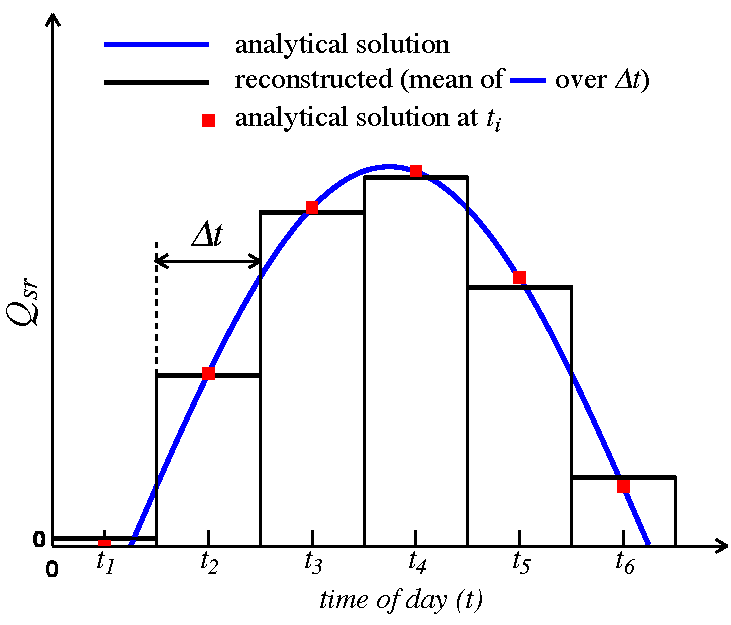
\includegraphics[width=0.8\textwidth]{./TexFiles/Figures/Fig_SBC_diurnal.pdf}
\caption{ \label{Fig_SBC_diurnal}    
Example of recontruction of the diurnal cycle variation of short wave flux  
from daily mean values. The reconstructed diurnal cycle (black line) is chosen 
as the mean value of the analytical cycle (blue line) over a time step, not 
as the mid time step value of the analytically cycle (red square). From \citet{Bernie_al_CD07}.}
\end{center}   \end{figure}
%>>>>>>>>>>>>>>>>>>>>>>>>>>>>

\cite{Bernie_al_JC05} have shown that to capture 90$\%$ of the diurnal variability of 
SST requires a vertical resolution in upper ocean of 1~m or better and a temporal resolution 
of the surface fluxes of 3~h or less. Unfortunately high frequency forcing fields are rare, 
not to say inexistent. Nevertheless, it is possible to obtain a reasonable diurnal cycle 
of the SST knowning only short wave flux (SWF) at high frequency \citep{Bernie_al_CD07}.
Furthermore, only the knowledge of daily mean value of SWF is needed, 
as higher frequency variations can be reconstructed from them, assuming that 
the diurnal cycle of SWF is a scaling of the top of the atmosphere diurnal cycle 
of incident SWF. The \cite{Bernie_al_CD07} reconstruction algorithm is available
in \NEMO by setting \np{ln\_dm2dc}~=~true (a \textit{\ngn{namsbc}} namelist variable) when using 
CORE bulk formulea (\np{ln\_blk\_core}~=~true) or the flux formulation (\np{ln\_flx}~=~true). 
The reconstruction is performed in the \mdl{sbcdcy} module. The detail of the algoritm used 
can be found in the appendix~A of \cite{Bernie_al_CD07}. The algorithm preserve the daily 
mean incomming SWF as the reconstructed SWF at a given time step is the mean value 
of the analytical cycle over this time step (Fig.\ref{Fig_SBC_diurnal}). 
The use of diurnal cycle reconstruction requires the input SWF to be daily 
($i.e.$ a frequency of 24 and a time interpolation set to true in \np{sn\_qsr} namelist parameter).
Furthermore, it is recommended to have a least 8 surface module time step per day,
that is  $\rdt \ \np{nn\_fsbc} < 10,800~s = 3~h$. An example of recontructed SWF 
is given in Fig.\ref{Fig_SBC_dcy} for a 12 reconstructed diurnal cycle, one every 2~hours 
(from 1am to 11pm).

%>>>>>>>>>>>>>>>>>>>>>>>>>>>>
\begin{figure}[!t]  \begin{center}
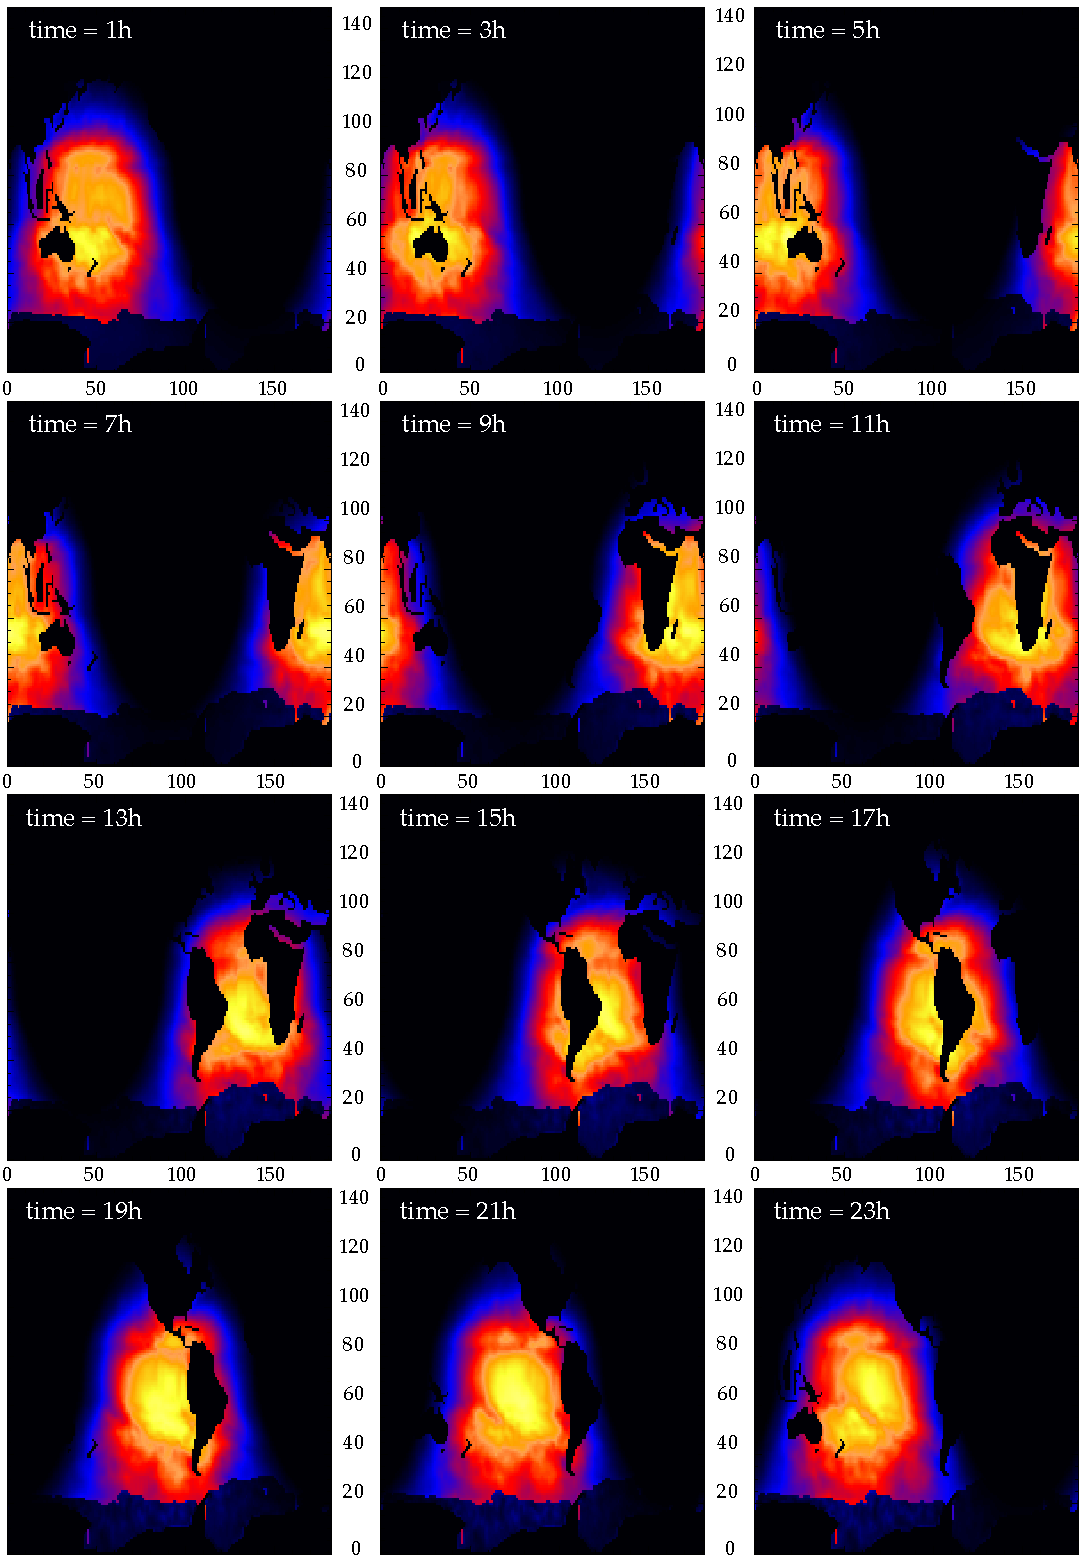
\includegraphics[width=0.7\textwidth]{./TexFiles/Figures/Fig_SBC_dcy.pdf}
\caption{ \label{Fig_SBC_dcy}   
Example of recontruction of the diurnal cycle variation of short wave flux  
from daily mean values on an ORCA2 grid with a time sampling of 2~hours (from 1am to 11pm). 
The display is on (i,j) plane. }
\end{center}   \end{figure}
%>>>>>>>>>>>>>>>>>>>>>>>>>>>>

Note also that the setting a diurnal cycle in SWF is highly recommended  when 
the top layer thickness approach 1~m or less, otherwise large error in SST can 
appear due to an inconsistency between the scale of the vertical resolution 
and the forcing acting on that scale.

% -------------------------------------------------------------------------------------------------------------
%        Rotation of vector pairs onto the model grid directions
% -------------------------------------------------------------------------------------------------------------
\subsection{Rotation of vector pairs onto the model grid directions}
\label{SBC_rotation}

When using a flux (\np{ln\_flx}=true) or bulk (\np{ln\_clio}=true or \np{ln\_core}=true) formulation, 
pairs of vector components can be rotated from east-north directions onto the local grid directions.  
This is particularly useful when interpolation on the fly is used since here any vectors are likely to be defined 
relative to a rectilinear grid.
To activate this option a non-empty string is supplied in the rotation pair column of the relevant namelist.
The eastward component must start with "U" and the northward component with "V".  
The remaining characters in the strings are used to identify which pair of components go together.
So for example, strings "U1" and "V1" next to "utau" and "vtau" would pair the wind stress components together
and rotate them on to the model grid directions; "U2" and "V2" could be used against a second pair of components, 
and so on.
The extra characters used in the strings are arbitrary.
The rot\_rep routine from the \mdl{geo2ocean} module is used to perform the rotation.

% -------------------------------------------------------------------------------------------------------------
%        Surface restoring to observed SST and/or SSS
% -------------------------------------------------------------------------------------------------------------
\subsection    [Surface restoring to observed SST and/or SSS (\textit{sbcssr})]
			{Surface restoring to observed SST and/or SSS (\mdl{sbcssr})}
\label{SBC_ssr}
%------------------------------------------namsbc_ssr----------------------------------------------------
\namdisplay{namsbc_ssr} 
%-------------------------------------------------------------------------------------------------------------

IOptions are defined through the  \ngn{namsbc\_ssr} namelist variables.
n forced mode using a flux formulation (\np{ln\_flx}~=~true), a 
feedback term \emph{must} be added to the surface heat flux $Q_{ns}^o$:
\begin{equation} \label{Eq_sbc_dmp_q}
Q_{ns} = Q_{ns}^o + \frac{dQ}{dT} \left( \left. T \right|_{k=1} - SST_{Obs} \right)
\end{equation}
where SST is a sea surface temperature field (observed or climatological), $T$ is 
the model surface layer temperature and $\frac{dQ}{dT}$ is a negative feedback 
coefficient usually taken equal to $-40~W/m^2/K$. For a $50~m$ 
mixed-layer depth, this value corresponds to a relaxation time scale of two months. 
This term ensures that if $T$ perfectly matches the supplied SST, then $Q$ is 
equal to $Q_o$. 

In the fresh water budget, a feedback term can also be added. Converted into an 
equivalent freshwater flux, it takes the following expression :

\begin{equation} \label{Eq_sbc_dmp_emp}
\textit{emp} = \textit{emp}_o + \gamma_s^{-1} e_{3t}  \frac{  \left(\left.S\right|_{k=1}-SSS_{Obs}\right)}
												         {\left.S\right|_{k=1}}
\end{equation}

where $\textit{emp}_{o }$ is a net surface fresh water flux (observed, climatological or an
atmospheric model product), \textit{SSS}$_{Obs}$ is a sea surface salinity (usually a time 
interpolation of the monthly mean Polar Hydrographic Climatology \citep{Steele2001}), 
$\left.S\right|_{k=1}$ is the model surface layer salinity and $\gamma_s$ is a negative 
feedback coefficient which is provided as a namelist parameter. Unlike heat flux, there is no 
physical justification for the feedback term in \ref{Eq_sbc_dmp_emp} as the atmosphere 
does not care about ocean surface salinity \citep{Madec1997}. The SSS restoring 
term should be viewed as a flux correction on freshwater fluxes to reduce the 
uncertainties we have on the observed freshwater budget.

% -------------------------------------------------------------------------------------------------------------
%        Handling of ice-covered area
% -------------------------------------------------------------------------------------------------------------
\subsection{Handling of ice-covered area  (\textit{sbcice\_...})}
\label{SBC_ice-cover}

The presence at the sea surface of an ice covered area modifies all the fluxes 
transmitted to the ocean. There are several way to handle sea-ice in the system 
depending on the value of the \np{nn{\_}ice} namelist parameter.  
\begin{description}
\item[nn{\_}ice = 0]  there will never be sea-ice in the computational domain. 
This is a typical namelist value used for tropical ocean domain. The surface fluxes 
are simply specified for an ice-free ocean. No specific things is done for sea-ice.
\item[nn{\_}ice = 1]  sea-ice can exist in the computational domain, but no sea-ice model 
is used. An observed ice covered area is read in a file. Below this area, the SST is 
restored to the freezing point and the heat fluxes are set to $-4~W/m^2$ ($-2~W/m^2$) 
in the northern (southern) hemisphere. The associated modification of the freshwater 
fluxes are done in such a way that the change in buoyancy fluxes remains zero. 
This prevents deep convection to occur when trying to reach the freezing point 
(and so ice covered area condition) while the SSS is too large. This manner of 
managing sea-ice area, just by using si IF case, is usually referred as the \textit{ice-if} 
model. It can be found in the \mdl{sbcice{\_}if} module.
\item[nn{\_}ice = 2 or more]  A full sea ice model is used. This model computes the 
ice-ocean fluxes, that are combined with the air-sea fluxes using the ice fraction of 
each model cell to provide the surface ocean fluxes. Note that the activation of a 
sea-ice model is is done by defining a CPP key (\key{lim2}, \key{lim3} or \key{cice}). 
The activation automatically overwrites the read value of nn{\_}ice to its appropriate 
value ($i.e.$ $2$ for LIM-2, $3$ for LIM-3 or $4$ for CICE).
\end{description}

% {Description of Ice-ocean interface to be added here or in LIM 2 and 3 doc ?}

\subsection   [Interface to CICE (\textit{sbcice\_cice})]
			{Interface to CICE (\mdl{sbcice\_cice})}
\label{SBC_cice}

It is now possible to couple a regional or global NEMO configuration (without AGRIF) to the CICE sea-ice
model by using \key{cice}.  The CICE code can be obtained from 
\href{http://oceans11.lanl.gov/trac/CICE/}{LANL} and the additional 'hadgem3' drivers will be required, 
even with the latest code release.  Input grid files consistent with those used in NEMO will also be needed, 
and CICE CPP keys \textbf{ORCA\_GRID}, \textbf{CICE\_IN\_NEMO} and \textbf{coupled} should be used (seek advice from UKMO 
if necessary).  Currently the code is only designed to work when using the CORE forcing option for NEMO (with
\textit{calc\_strair~=~true} and \textit{calc\_Tsfc~=~true} in the CICE name-list), or alternatively when NEMO 
is coupled to the HadGAM3 atmosphere model (with \textit{calc\_strair~=~false} and \textit{calc\_Tsfc~=~false}).
The code is intended to be used with \np{nn\_fsbc} set to 1 (although coupling ocean and ice less frequently 
should work, it is possible the calculation of some of the ocean-ice fluxes needs to be modified slightly - the
user should check that results are not significantly different to the standard case).

There are two options for the technical coupling between NEMO and CICE.  The standard version allows
complete flexibility for the domain decompositions in the individual models, but this is at the expense of global
gather and scatter operations in the coupling which become very expensive on larger numbers of processors. The
alternative option (using \key{nemocice\_decomp} for both NEMO and CICE) ensures that the domain decomposition is
identical in both models (provided domain parameters are set appropriately, and 
\textit{processor\_shape~=~square-ice} and \textit{distribution\_wght~=~block} in the CICE name-list) and allows
much more efficient direct coupling on individual processors.  This solution scales much better although it is at 
the expense of having more idle CICE processors in areas where there is no sea ice.

% -------------------------------------------------------------------------------------------------------------
%        Freshwater budget control 
% -------------------------------------------------------------------------------------------------------------
\subsection   [Freshwater budget control (\textit{sbcfwb})]
			{Freshwater budget control (\mdl{sbcfwb})}
\label{SBC_fwb}

For global ocean simulation it can be useful to introduce a control of the mean sea 
level in order to prevent unrealistic drift of the sea surface height due to inaccuracy 
in the freshwater fluxes. In \NEMO, two way of controlling the the freshwater budget. 
\begin{description}
\item[\np{nn\_fwb}=0]  no control at all. The mean sea level is free to drift, and will 
certainly do so.
\item[\np{nn\_fwb}=1]  global mean \textit{emp} set to zero at each model time step. 
%Note that with a sea-ice model, this technique only control the mean sea level with linear free surface (\key{vvl} not defined) and no mass flux between ocean and ice (as it is implemented in the current ice-ocean coupling). 
\item[\np{nn\_fwb}=2]  freshwater budget is adjusted from the previous year annual 
mean budget which is read in the \textit{EMPave\_old.dat} file. As the model uses the 
Boussinesq approximation, the annual mean fresh water budget is simply evaluated 
from the change in the mean sea level at January the first and saved in the 
\textit{EMPav.dat} file. 
\end{description}

% -------------------------------------------------------------------------------------------------------------
%        Neutral Drag Coefficient from external wave model
% -------------------------------------------------------------------------------------------------------------
\subsection   [Neutral drag coefficient from external wave model (\textit{sbcwave})]
                        {Neutral drag coefficient from external wave model (\mdl{sbcwave})}
\label{SBC_wave}
%------------------------------------------namwave----------------------------------------------------
\namdisplay{namsbc_wave}
%-------------------------------------------------------------------------------------------------------------
\begin{description}

\item [??] In order to read a neutral drag coeff, from an external data source (i.e. a wave model), the 
logical variable \np{ln\_cdgw}
 in $namsbc$ namelist must be defined ${.true.}$. 
The \mdl{sbcwave} module containing the routine \np{sbc\_wave} reads the
namelist \ngn{namsbc\_wave} (for external data names, locations, frequency, interpolation and all 
the miscellanous options allowed by Input Data generic Interface see \S\ref{SBC_input}) 
and a 2D field of neutral drag coefficient. Then using the routine 
TURB\_CORE\_1Z or TURB\_CORE\_2Z, and starting from the neutral drag coefficent provided, the drag coefficient is computed according 
to stable/unstable conditions of the air-sea interface following \citet{Large_Yeager_Rep04}.

\end{description}

% Griffies doc:
% When running ocean-ice simulations, we are not explicitly representing land processes, such as rivers, catchment areas, snow accumulation, etc. However, to reduce model drift, it is important to balance the hydrological cycle in ocean-ice models. We thus need to prescribe some form of global normalization to the precipitation minus evaporation plus river runoff. The result of the normalization should be a global integrated zero net water input to the ocean-ice system over a chosen time scale. 
%How often the normalization is done is a matter of choice. In mom4p1, we choose to do so at each model time step, so that there is always a zero net input of water to the ocean-ice system. Others choose to normalize over an annual cycle, in which case the net imbalance over an annual cycle is used to alter the subsequent year�s water budget in an attempt to damp the annual water imbalance. Note that the annual budget approach may be inappropriate with interannually varying precipitation forcing. 
%When running ocean-ice coupled models, it is incorrect to include the water transport between the ocean and ice models when aiming to balance the hydrological cycle. The reason is that it is the sum of the water in the ocean plus ice that should be balanced when running ocean-ice models, not the water in any one sub-component. As an extreme example to illustrate the issue, consider an ocean-ice model with zero initial sea ice. As the ocean-ice model spins up, there should be a net accumulation of water in the growing sea ice, and thus a net loss of water from the ocean. The total water contained in the ocean plus ice system is constant, but there is an exchange of water between the subcomponents. This exchange should not be part of the normalization used to balance the hydrological cycle in ocean-ice models. 


			% Surface Boundary Conditions

% ================================================================
% Chapter � Lateral Boundary Condition (LBC) 
% ================================================================
\chapter{Lateral Boundary Condition (LBC) }
\label{LBC}
\minitoc

\newpage
$\ $\newline    % force a new ligne


%gm% add here introduction to this chapter

% ================================================================
% Boundary Condition at the Coast
% ================================================================
\section{Boundary Condition at the Coast (\np{rn\_shlat})}
\label{LBC_coast}
%--------------------------------------------nam_lbc-------------------------------------------------------
\namdisplay{namlbc} 
%--------------------------------------------------------------------------------------------------------------

%The lateral ocean boundary conditions contiguous to coastlines are Neumann conditions for heat and salt (no flux across boundaries) and Dirichlet conditions for momentum (ranging from free-slip to "strong" no-slip). They are handled automatically by the mask system (see \S\ref{DOM_msk}). 

%OPA allows land and topography grid points in the computational domain due to the presence of continents or islands, and includes the use of a full or partial step representation of bottom topography. The computation is performed over the whole domain, i.e. we do not try to restrict the computation to ocean-only points. This choice has two motivations. Firstly, working on ocean only grid points overloads the code and harms the code readability. Secondly, and more importantly, it drastically reduces the vector portion of the computation, leading to a dramatic increase of CPU time requirement on vector computers.  The current section describes how the masking affects the computation of the various terms of the equations with respect to the boundary condition at solid walls. The process of defining which areas are to be masked is described in \S\ref{DOM_msk}.

Options are defined through the \ngn{namlbc} namelist variables.
The discrete representation of a domain with complex boundaries (coastlines and 
bottom topography) leads to arrays that include large portions where a computation 
is not required as the model variables remain at zero. Nevertheless, vectorial 
supercomputers are far more efficient when computing over a whole array, and the 
readability of a code is greatly improved when boundary conditions are applied in 
an automatic way rather than by a specific computation before or after each 
computational loop. An efficient way to work over the whole domain while specifying 
the boundary conditions, is to use multiplication by mask arrays in the computation. 
A mask array is a matrix whose elements are $1$ in the ocean domain and $0$ 
elsewhere. A simple multiplication of a variable by its own mask ensures that it will 
remain zero over land areas. Since most of the boundary conditions consist of a 
zero flux across the solid boundaries, they can be simply applied by multiplying 
variables by the correct mask arrays, $i.e.$ the mask array of the grid point where 
the flux is evaluated. For example, the heat flux in the \textbf{i}-direction is evaluated 
at $u$-points. Evaluating this quantity as,

\begin{equation} \label{Eq_lbc_aaaa}
\frac{A^{lT} }{e_1 }\frac{\partial T}{\partial i}\equiv \frac{A_u^{lT} 
}{e_{1u} } \; \delta _{i+1 / 2} \left[ T \right]\;\;mask_u 
\end{equation}
(where mask$_{u}$ is the mask array at a $u$-point) ensures that the heat flux is 
zero inside land and at the boundaries, since mask$_{u}$ is zero at solid boundaries 
which in this case are defined at $u$-points (normal velocity $u$ remains zero at 
the coast) (Fig.~\ref{Fig_LBC_uv}). 

%>>>>>>>>>>>>>>>>>>>>>>>>>>>>
\begin{figure}[!t]     \begin{center}
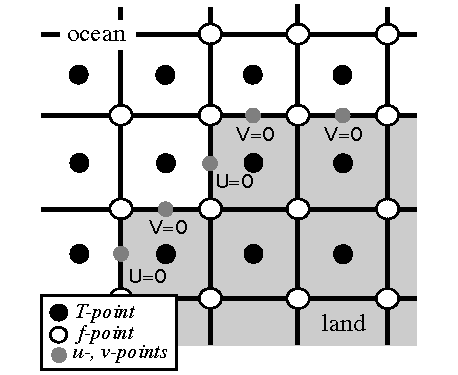
\includegraphics[width=0.90\textwidth]{./TexFiles/Figures/Fig_LBC_uv.pdf}
\caption{  \label{Fig_LBC_uv}
Lateral boundary (thick line) at T-level. The velocity normal to the boundary is set to zero.}
\end{center}   \end{figure}
%>>>>>>>>>>>>>>>>>>>>>>>>>>>>

For momentum the situation is a bit more complex as two boundary conditions 
must be provided along the coast (one each for the normal and tangential velocities). 
The boundary of the ocean in the C-grid is defined by the velocity-faces. 
For example, at a given $T$-level, the lateral boundary (a coastline or an intersection 
with the bottom topography) is made of segments joining $f$-points, and normal 
velocity points are located between two $f-$points (Fig.~\ref{Fig_LBC_uv}). 
The boundary condition on the normal velocity (no flux through solid boundaries) 
can thus be easily implemented using the mask system. The boundary condition 
on the tangential velocity requires a more specific treatment. This boundary 
condition influences the relative vorticity and momentum diffusive trends, and is 
required in order to compute the vorticity at the coast. Four different types of 
lateral boundary condition are available, controlled by the value of the \np{rn\_shlat} 
namelist parameter. (The value of the mask$_{f}$ array along the coastline is set 
equal to this parameter.) These are:

%>>>>>>>>>>>>>>>>>>>>>>>>>>>>
\begin{figure}[!p] \begin{center}
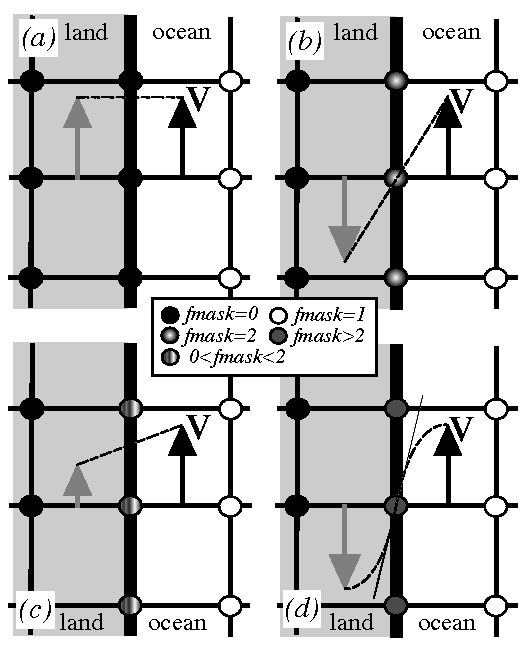
\includegraphics[width=0.90\textwidth]{./TexFiles/Figures/Fig_LBC_shlat.pdf}
\caption{     \label{Fig_LBC_shlat} 
lateral boundary condition (a) free-slip ($rn\_shlat=0$) ; (b) no-slip ($rn\_shlat=2$) 
; (c) "partial" free-slip ($0<rn\_shlat<2$) and (d) "strong" no-slip ($2<rn\_shlat$). 
Implied "ghost" velocity inside land area is display in grey. }
\end{center}    \end{figure}
%>>>>>>>>>>>>>>>>>>>>>>>>>>>>

\begin{description}

\item[free-slip boundary condition (\np{rn\_shlat}=0): ]  the tangential velocity at the 
coastline is equal to the offshore velocity, $i.e.$ the normal derivative of the 
tangential velocity is zero at the coast, so the vorticity: mask$_{f}$ array is set 
to zero inside the land and just at the coast (Fig.~\ref{Fig_LBC_shlat}-a).

\item[no-slip boundary condition (\np{rn\_shlat}=2): ] the tangential velocity vanishes 
at the coastline. Assuming that the tangential velocity decreases linearly from 
the closest ocean velocity grid point to the coastline, the normal derivative is 
evaluated as if the velocities at the closest land velocity gridpoint and the closest 
ocean velocity gridpoint were of the same magnitude but in the opposite direction 
(Fig.~\ref{Fig_LBC_shlat}-b). Therefore, the vorticity along the coastlines is given by: 

\begin{equation*}
\zeta \equiv 2 \left(\delta_{i+1/2} \left[e_{2v} v \right] - \delta_{j+1/2} \left[e_{1u} u \right] \right) / \left(e_{1f} e_{2f} \right) \ ,
\end{equation*}
where $u$ and $v$ are masked fields. Setting the mask$_{f}$ array to $2$ along 
the coastline provides a vorticity field computed with the no-slip boundary condition, 
simply by multiplying it by the mask$_{f}$ :
\begin{equation} \label{Eq_lbc_bbbb}
\zeta \equiv \frac{1}{e_{1f} {\kern 1pt}e_{2f} }\left( {\delta _{i+1/2} 
\left[ {e_{2v} \,v} \right]-\delta _{j+1/2} \left[ {e_{1u} \,u} \right]} 
\right)\;\mbox{mask}_f 
\end{equation}

\item["partial" free-slip boundary condition (0$<$\np{rn\_shlat}$<$2): ] the tangential 
velocity at the coastline is smaller than the offshore velocity, $i.e.$ there is a lateral 
friction but not strong enough to make the tangential velocity at the coast vanish 
(Fig.~\ref{Fig_LBC_shlat}-c). This can be selected by providing a value of mask$_{f}$ 
strictly inbetween $0$ and $2$.

\item["strong" no-slip boundary condition (2$<$\np{rn\_shlat}): ] the viscous boundary 
layer is assumed to be smaller than half the grid size (Fig.~\ref{Fig_LBC_shlat}-d). 
The friction is thus larger than in the no-slip case.

\end{description}

Note that when the bottom topography is entirely represented by the $s$-coor-dinates 
(pure $s$-coordinate), the lateral boundary condition on tangential velocity is of much 
less importance as it is only applied next to the coast where the minimum water depth 
can be quite shallow.

The alternative numerical implementation of the no-slip boundary conditions for an 
arbitrary coast line of \citet{Shchepetkin1996} is also available through the 
\key{noslip\_accurate} CPP key. It is based on a fourth order evaluation of the shear at the 
coast which, in turn, allows a true second order scheme in the interior of the domain 
($i.e.$ the numerical boundary scheme simulates the truncation error of the numerical 
scheme used in the interior of the domain). \citet{Shchepetkin1996} found that such a 
technique considerably improves the quality of the numerical solution. In \NEMO, such 
spectacular improvements have not been found in the half-degree global ocean 
(ORCA05), but significant reductions of numerically induced coastal upwellings were 
found in an eddy resolving simulation of the Alboran Sea \citep{Olivier_PhD01}. 
Nevertheless, since a no-slip boundary condition is not recommended in an eddy 
permitting or resolving simulation \citep{Penduff_al_OS07}, the use of this option is also 
not recommended.

In practice, the no-slip accurate option changes the way the curl is evaluated at the 
coast (see \mdl{divcur} module), and requires the nature of each coastline grid point 
(convex or concave corners, straight north-south or east-west coast) to be specified.  
This is performed in routine \rou{dom\_msk\_nsa} in the \mdl{domask} module.

% ================================================================
% Boundary Condition around the Model Domain
% ================================================================
\section{Model Domain Boundary Condition (\np{jperio})}
\label{LBC_jperio}

At the model domain boundaries several choices are offered: closed, cyclic east-west, 
south symmetric across the equator, a north-fold, and combination closed-north fold 
or cyclic-north-fold. The north-fold boundary condition is associated with the 3-pole ORCA mesh. 

% -------------------------------------------------------------------------------------------------------------
%        Closed, cyclic, south symmetric (\np{jperio} = 0, 1 or 2) 
% -------------------------------------------------------------------------------------------------------------
\subsection{Closed, cyclic, south symmetric (\np{jperio} = 0, 1 or 2)}
\label{LBC_jperio012}

The choice of closed, cyclic or symmetric model domain boundary condition is made 
by setting \np{jperio} to 0, 1 or 2 in namelist \ngn{namcfg}. Each time such a boundary 
condition is needed, it is set by a call to routine \mdl{lbclnk}. The computation of 
momentum and tracer trends proceeds from $i=2$ to $i=jpi-1$ and from $j=2$ to 
$j=jpj-1$, $i.e.$ in the model interior. To choose a lateral model boundary condition 
is to specify the first and last rows and columns of the model variables. 

\begin{description}

\item[For closed boundary (\textit{jperio=0})], solid walls are imposed at all model 
boundaries: first and last rows and columns are set to zero.

\item[For cyclic east-west boundary (\textit{jperio=1})], first and last rows are set 
to zero (closed) whilst the first column is set to the value of the last-but-one column 
and the last column to the value of the second one (Fig.~\ref{Fig_LBC_jperio}-a). 
Whatever flows out of the eastern (western) end of the basin enters the western 
(eastern) end. Note that there is no option for north-south cyclic or for doubly 
cyclic cases.

\item[For symmetric boundary condition across the equator (\textit{jperio=2})], 
last rows, and first and last columns are set to zero (closed). The row of symmetry 
is chosen to be the $u$- and $T-$points equator line ($j=2$, i.e. at the southern 
end of the domain). For arrays defined at $u-$ or $T-$points, the first row is set 
to the value of the third row while for most of $v$- and $f$-point arrays ($v$, $\zeta$, 
$j\psi$, but \gmcomment{not sure why this is "but"} scalar arrays such as eddy coefficients) 
the first row is set to minus the value of the second row (Fig.~\ref{Fig_LBC_jperio}-b). 
Note that this boundary condition is not yet available for the case of a massively 
parallel computer (\textbf{key{\_}mpp} defined).

\end{description}

%>>>>>>>>>>>>>>>>>>>>>>>>>>>>
\begin{figure}[!t]     \begin{center}
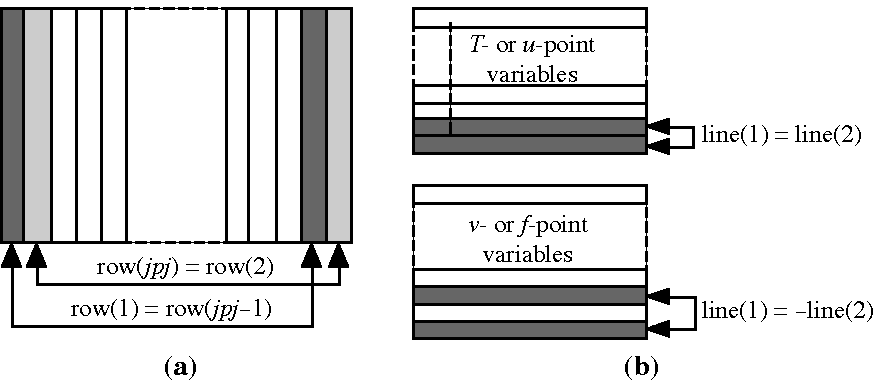
\includegraphics[width=1.0\textwidth]{./TexFiles/Figures/Fig_LBC_jperio.pdf}
\caption{    \label{Fig_LBC_jperio}
setting of (a) east-west cyclic  (b) symmetric across the equator boundary conditions.}
\end{center}   \end{figure}
%>>>>>>>>>>>>>>>>>>>>>>>>>>>>

% -------------------------------------------------------------------------------------------------------------
%        North fold (\textit{jperio = 3 }to $6)$ 
% -------------------------------------------------------------------------------------------------------------
\subsection{North-fold (\textit{jperio = 3 }to $6)$ }
\label{LBC_north_fold}

The north fold boundary condition has been introduced in order to handle the north 
boundary of a three-polar ORCA grid. Such a grid has two poles in the northern hemisphere. 
\colorbox{yellow}{to be completed...}

%>>>>>>>>>>>>>>>>>>>>>>>>>>>>
\begin{figure}[!t]    \begin{center}
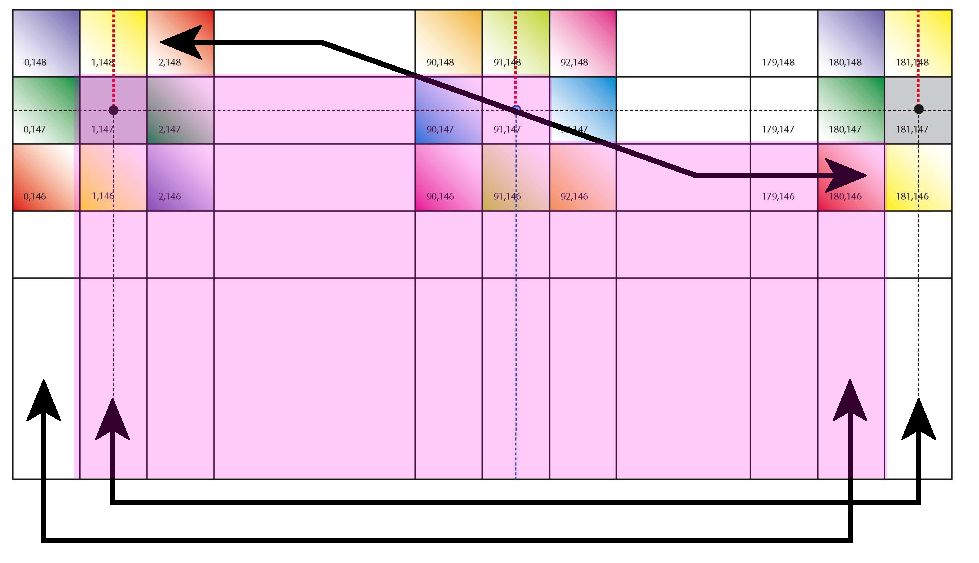
\includegraphics[width=0.90\textwidth]{./TexFiles/Figures/Fig_North_Fold_T.pdf}
\caption{    \label{Fig_North_Fold_T} 
North fold boundary with a $T$-point pivot and cyclic east-west boundary condition 
($jperio=4$), as used in ORCA 2, 1/4, and 1/12. Pink shaded area corresponds 
to the inner domain mask (see text). }
\end{center}   \end{figure}
%>>>>>>>>>>>>>>>>>>>>>>>>>>>>

% ====================================================================
% Exchange with neighbouring processors 
% ====================================================================
\section  [Exchange with neighbouring processors (\textit{lbclnk}, \textit{lib\_mpp})]
		{Exchange with neighbouring processors (\mdl{lbclnk}, \mdl{lib\_mpp})}
\label{LBC_mpp}

For massively parallel processing (mpp), a domain decomposition method is used. 
The basic idea of the method is to split the large computation domain of a numerical 
experiment into several smaller domains and solve the set of equations by addressing 
independent local problems. Each processor has its own local memory and computes 
the model equation over a subdomain of the whole model domain. The subdomain 
boundary conditions are specified through communications between processors 
which are organized by explicit statements (message passing method). 

A big advantage is that the method does not need many modifications of the initial 
FORTRAN code. From the modeller's point of view, each sub domain running on 
a processor is identical to the "mono-domain" code. In addition, the programmer 
manages the communications between subdomains, and the code is faster when 
the number of processors is increased. The porting of OPA code on an iPSC860 
was achieved during Guyon's PhD [Guyon et al. 1994, 1995] in collaboration with 
CETIIS and ONERA. The implementation in the operational context and the studies 
of performance on a T3D and T3E Cray computers have been made in collaboration 
with IDRIS and CNRS. The present implementation is largely inspired by Guyon's 
work  [Guyon 1995].

The parallelization strategy is defined by the physical characteristics of the 
ocean model. Second order finite difference schemes lead to local discrete 
operators that depend at the very most on one neighbouring point. The only 
non-local computations concern the vertical physics (implicit diffusion, 1.5 
turbulent closure scheme, ...) (delocalization over the whole water column), 
and the solving of the elliptic equation associated with the surface pressure 
gradient computation (delocalization over the whole horizontal domain). 
Therefore, a pencil strategy is used for the data sub-structuration 
\gmcomment{no idea what this means!}
: the 3D initial domain is laid out on local processor 
memories following a 2D horizontal topological splitting. Each sub-domain 
computes its own surface and bottom boundary conditions and has a side 
wall overlapping interface which defines the lateral boundary conditions for 
computations in the inner sub-domain. The overlapping area consists of the 
two rows at each edge of the sub-domain. After a computation, a communication 
phase starts: each processor sends to its neighbouring processors the update 
values of the points corresponding to the interior overlapping area to its 
neighbouring sub-domain (i.e. the innermost of the two overlapping rows). 
The communication is done through message passing. Usually the parallel virtual 
language, PVM, is used as it is a standard language available on  nearly  all 
MPP computers. More specific languages (i.e. computer dependant languages) 
can be easily used to speed up the communication, such as SHEM on a T3E 
computer. The data exchanges between processors are required at the very 
place where lateral domain boundary conditions are set in the mono-domain 
computation (\S III.10-c): the lbc\_lnk routine which manages such conditions 
is substituted by mpplnk.F or mpplnk2.F routine when running on an MPP 
computer (\key{mpp\_mpi} defined). It has to be pointed out that when using 
the MPP version of the model, the east-west cyclic boundary condition is done 
implicitly, whilst the south-symmetric boundary condition option is not available.

%>>>>>>>>>>>>>>>>>>>>>>>>>>>>
\begin{figure}[!t]    \begin{center}
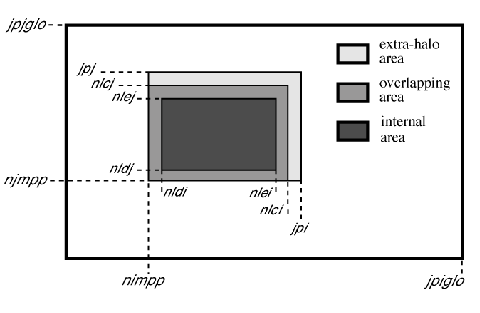
\includegraphics[width=0.90\textwidth]{./TexFiles/Figures/Fig_mpp.pdf}
\caption{   \label{Fig_mpp} 
Positioning of a sub-domain when massively parallel processing is used. }
\end{center}   \end{figure}
%>>>>>>>>>>>>>>>>>>>>>>>>>>>>

In the standard version of the OPA model, the splitting is regular and arithmetic.
 the i-axis is divided by \jp{jpni} and the j-axis by \jp{jpnj} for a number of processors 
 \jp{jpnij} most often equal to $jpni \times jpnj$ (model parameters set in 
 \mdl{par\_oce}). Each processor is independent and without message passing 
 or synchronous process 
 \gmcomment{how does a synchronous process relate to this?}, 
 programs run alone and access just its own local memory. For this reason, the 
 main model dimensions are now the local dimensions of the subdomain (pencil) 
 that are named \jp{jpi}, \jp{jpj}, \jp{jpk}. These dimensions include the internal 
 domain and the overlapping rows. The number of rows to exchange (known as 
 the halo) is usually set to one (\jp{jpreci}=1, in \mdl{par\_oce}). The whole domain 
 dimensions are named \np{jpiglo}, \np{jpjglo} and \jp{jpk}. The relationship between 
 the whole domain and a sub-domain is:
\begin{eqnarray} 
      jpi & = & ( jpiglo-2*jpreci + (jpni-1) ) / jpni + 2*jpreci  \nonumber \\
      jpj & = & ( jpjglo-2*jprecj + (jpnj-1) ) / jpnj + 2*jprecj  \label{Eq_lbc_jpi}
\end{eqnarray}
where \jp{jpni}, \jp{jpnj} are the number of processors following the i- and j-axis.

\colorbox{yellow}{Figure IV.3: example of a domain splitting with 9 processors and 
no east-west cyclic boundary conditions.}

One also defines variables nldi and nlei which correspond to the internal 
domain bounds, and the variables nimpp and njmpp which are the position 
of the (1,1) grid-point in the global domain. An element of $T_{l}$, a local array 
(subdomain) corresponds to an element of $T_{g}$, a global array 
(whole domain) by the relationship: 
\begin{equation} \label{Eq_lbc_nimpp}
T_{g} (i+nimpp-1,j+njmpp-1,k) = T_{l} (i,j,k),
\end{equation}
with  $1 \leq i \leq jpi$, $1  \leq j \leq jpj $ , and  $1  \leq k \leq jpk$.

Processors are numbered from 0 to $jpnij-1$, the number is saved in the variable 
nproc. In the standard version, a processor has no more than four neighbouring 
processors named nono (for north), noea (east), noso (south) and nowe (west) 
and two variables, nbondi and nbondj, indicate the relative position of the processor 
\colorbox{yellow}{(see Fig.IV.3)}:
\begin{itemize}
\item 		nbondi = -1 	an east neighbour, no west processor,
\item 		nbondi =  0	an east neighbour, a west neighbour,
\item 		nbondi =  1 	no east processor, a west neighbour,
\item 		nbondi =  2 	no splitting following the i-axis.
\end{itemize}
During the simulation, processors exchange data with their neighbours. 
If there is effectively a neighbour, the processor receives variables from this 
processor on its overlapping row, and sends the data issued from internal 
domain corresponding to the overlapping row of the other processor.
		 
\colorbox{yellow}{Figure IV.4: pencil splitting with the additional outer halos }


The \NEMO model computes equation terms with the help of mask arrays (0 on land 
points and 1 on sea points). It is easily readable and very efficient in the context of 
a computer with vectorial architecture. However, in the case of a scalar processor, 
computations over the land regions become more expensive in terms of CPU time. 
It is worse when we use a complex configuration with a realistic bathymetry like the 
global ocean where more than 50 \% of points are land points. For this reason, a 
pre-processing tool can be used to choose the mpp domain decomposition with a 
maximum number of only land points processors, which can then be eliminated. 
(For example, the mpp\_optimiz tools, available from the DRAKKAR web site.) 
This optimisation is dependent on the specific bathymetry employed. The user 
then chooses optimal parameters \jp{jpni}, \jp{jpnj} and \jp{jpnij} with 
$jpnij < jpni \times jpnj$, leading to the elimination of $jpni \times jpnj - jpnij$ 
land processors. When those parameters are specified in module \mdl{par\_oce}, 
the algorithm in the \rou{inimpp2} routine sets each processor's parameters (nbound, 
nono, noea,...) so that the land-only processors are not taken into account. 

\colorbox{yellow}{Note that the inimpp2 routine is general so that the original inimpp 
routine should be suppressed from the code.}

When land processors are eliminated, the value corresponding to these locations in 
the model output files is zero. Note that this is a problem for a mesh output file written 
by such a model configuration, because model users often divide by the scale factors 
($e1t$, $e2t$, etc) and do not expect the grid size to be zero, even on land. It may be 
best not to eliminate land processors when running the model especially to write the 
mesh files as outputs (when \np{nn\_msh} namelist parameter differs from 0).
%%
\gmcomment{Steven : dont understand this, no land processor means no output file 
covering this part of globe; its only when files are stitched together into one that you 
can leave a hole}
%%

%>>>>>>>>>>>>>>>>>>>>>>>>>>>>
\begin{figure}[!ht]     \begin{center}
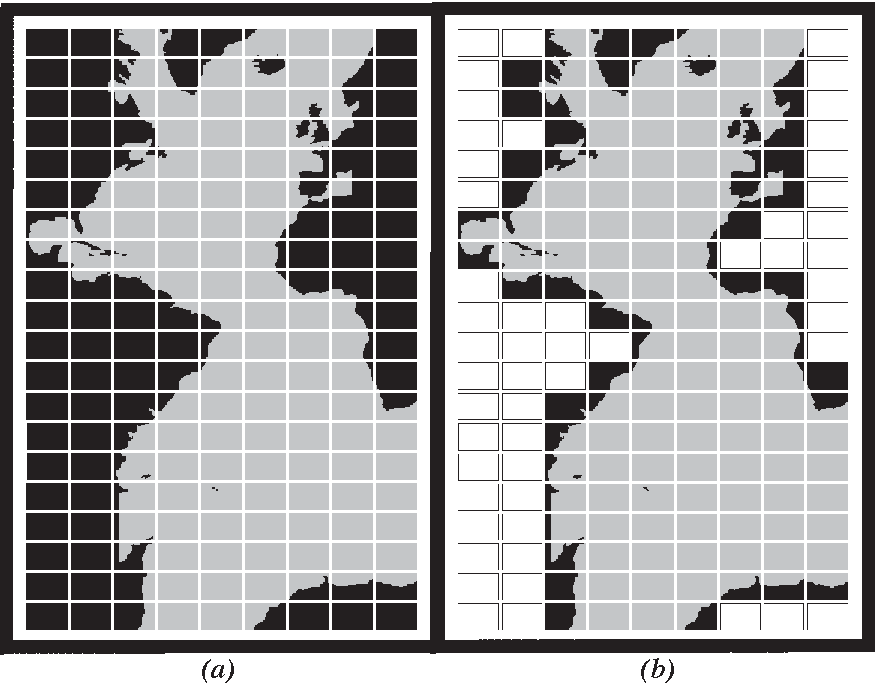
\includegraphics[width=0.90\textwidth]{./TexFiles/Figures/Fig_mppini2.pdf}
\caption {    \label{Fig_mppini2}
Example of Atlantic domain defined for the CLIPPER projet. Initial grid is 
composed of 773 x 1236 horizontal points. 
(a) the domain is split onto 9 \time 20 subdomains (jpni=9, jpnj=20). 
52 subdomains are land areas. 
(b) 52 subdomains are eliminated (white rectangles) and the resulting number 
of processors really used during the computation is jpnij=128.}
\end{center}   \end{figure}
%>>>>>>>>>>>>>>>>>>>>>>>>>>>>


% ================================================================
% Open Boundary Conditions 
% ================================================================
\section{Open Boundary Conditions (\key{obc}) (OBC)}
\label{LBC_obc}
%-----------------------------------------nam_obc  -------------------------------------------
%-    nobc_dta    =    0     !  = 0 the obc data are equal to the initial state
%-                           !  = 1 the obc data are read in 'obc   .dta' files
%-    rn_dpein      =    1.    !  ???
%-    rn_dpwin      =    1.    !  ???
%-    rn_dpnin      =   30.    !  ???
%-    rn_dpsin      =    1.    !  ???
%-    rn_dpeob      = 1500.    !  time relaxation (days) for the east  open boundary
%-    rn_dpwob      =   15.    !    "        "           for the west  open boundary
%-    rn_dpnob      =  150.    !    "        "           for the north open boundary
%-    rn_dpsob      =   15.    !    "        "           for the south open boundary
%-    ln_obc_clim = .true.   !  climatological obc data files (default T)
%-    ln_vol_cst  = .true.   !  total volume conserved
\namdisplay{namobc} 

It is often necessary to implement a model configuration limited to an oceanic 
region or a basin, which communicates with the rest of the global ocean through 
''open boundaries''. As stated by \citet{Roed1986}, an open boundary is a 
computational border where the aim of the calculations is to allow the perturbations 
generated inside the computational domain to leave it without deterioration of the 
inner model solution. However, an open boundary also has to let information from 
the outer ocean enter the model and should support inflow and outflow conditions. 

The open boundary package OBC is the first open boundary option developed in 
NEMO (originally in OPA8.2). It allows the user to 
\begin{itemize}
\item tell the model that a boundary is ''open'' and not closed by a wall, for example 
by modifying the calculation of the divergence of velocity there;
\item impose values of tracers and velocities at that boundary (values which may 
be taken from a climatology): this is the``fixed OBC'' option. 
\item calculate boundary values by a sophisticated algorithm combining radiation 
and relaxation (``radiative OBC'' option)
\end{itemize}

Options are defined through the \ngn{namobc} namelist variables.
The package resides in the OBC directory. It is described here in four parts: the 
boundary geometry (parameters to be set in \mdl{obc\_par}), the forcing data at 
the boundaries (module \mdl{obcdta}),  the radiation algorithm involving the 
namelist and module \mdl{obcrad}, and a brief presentation of boundary update 
and restart files.

%----------------------------------------------
\subsection{Boundary geometry}
\label{OBC_geom}
%
First one has to realize that open boundaries may not necessarily be located 
at the extremities of the computational domain. They may exist in the middle 
of the domain, for example at Gibraltar Straits if one wants to avoid including 
the Mediterranean in an Atlantic domain. This flexibility has been found necessary 
for the CLIPPER project \citep{Treguier_al_JGR01}. Because of the complexity of the 
geometry of ocean basins, it may even be necessary to have more than one 
''west'' open boundary, more than one ''north'', etc. This is not possible with 
the OBC option: only one open boundary of each kind, west, east, south and 
north is allowed; these names refer to the grid geometry (not to the direction 
of the geographical ''west'', ''east'', etc).

The open boundary geometry is set by a series of parameters in the module 
\mdl{obc\_par}. For an eastern open boundary, parameters are \jp{lp\_obc\_east} 
(true if an east open boundary exists), \jp{jpieob} the $i$-index along which 
the eastern open boundary (eob) is located, \jp{jpjed} the $j$-index at which 
it starts, and \jp{jpjef} the $j$-index where it ends (note $d$ is for ''d\'{e}but'' 
and $f$ for ''fin'' in French). Similar parameters exist for the west, south and 
north cases (Table~\ref{Tab_obc_param}).


%--------------------------------------------------TABLE--------------------------------------------------
\begin{table}[htbp]     \begin{center}    \begin{tabular}{|l|c|c|c|}
\hline
Boundary and  & Constant index  & Starting index (d\'{e}but) & Ending index (fin) \\
Logical flag  &                 &                            &                     \\
\hline
West          & \jp{jpiwob} $>= 2$         &  \jp{jpjwd}$>= 2$          &  \jp{jpjwf}<= \np{jpjglo}-1 \\
lp\_obc\_west & $i$-index of a $u$ point   & $j$ of a $T$ point   &$j$ of a $T$ point \\
\hline
East            & \jp{jpieob}$<=$\np{jpiglo}-2&\jp{jpjed} $>= 2$         & \jp{jpjef}$<=$ \np{jpjglo}-1 \\
 lp\_obc\_east  & $i$-index of a $u$ point    & $j$ of a $T$ point & $j$ of a $T$ point \\
\hline
South           & \jp{jpjsob} $>= 2$         & \jp{jpisd} $>= 2$          & \jp{jpisf}$<=$\np{jpiglo}-1 \\
lp\_obc\_south  & $j$-index of a $v$ point   & $i$ of a $T$ point   & $i$ of a $T$ point \\
\hline
North           & \jp{jpjnob} $<=$ \np{jpjglo}-2& \jp{jpind} $>= 2$        & \jp{jpinf}$<=$\np{jpiglo}-1 \\
lp\_obc\_north  & $j$-index of a $v$ point      & $i$  of a $T$ point & $i$ of a $T$ point \\
\hline
\end{tabular}    \end{center}
\caption{     \label{Tab_obc_param}
Names of different indices relating to the open boundaries. In the case 
of a completely open ocean domain with four ocean boundaries, the parameters 
take exactly the values indicated.}
\end{table}
%------------------------------------------------------------------------------------------------------------

The open boundaries must be along coordinate lines. On the C-grid, the boundary 
itself is along a line of normal velocity points: $v$ points for a zonal open boundary 
(the south or north one), and $u$ points for a meridional open boundary (the west 
or east one). Another constraint is that there still must be a row of masked points 
all around the domain, as if the domain were a closed basin (unless periodic conditions 
are used together with open boundary conditions). Therefore, an open boundary 
cannot be located at the first/last index, namely, 1, \jp{jpiglo} or \jp{jpjglo}. Also, 
the open boundary algorithm involves calculating the normal velocity points situated 
just on the boundary, as well as the tangential velocity and temperature and salinity 
just outside the boundary. This means that for a west/south boundary, normal 
velocities and temperature are calculated at the same index \jp{jpiwob} and 
\jp{jpjsob}, respectively. For an east/north boundary, the normal velocity is 
calculated at index \jp{jpieob} and \jp{jpjnob}, but the ``outside'' temperature is 
at index \jp{jpieob}+1 and \jp{jpjnob}+1. This means that \jp{jpieob}, \jp{jpjnob} 
cannot be bigger than \jp{jpiglo}-2, \jp{jpjglo}-2. 


The starting and ending indices are to be thought of as $T$ point indices: in many 
cases they indicate the first land $T$-point, at the extremity of an open boundary 
(the coast line follows the $f$ grid points, see Fig.~\ref{Fig_obc_north} for an example 
of a northern open boundary). All indices are relative to the global domain. In the 
free surface case it is possible to have ``ocean corners'', that is, an open boundary 
starting and ending in the ocean.

%>>>>>>>>>>>>>>>>>>>>>>>>>>>>
\begin{figure}[!t]     \begin{center}
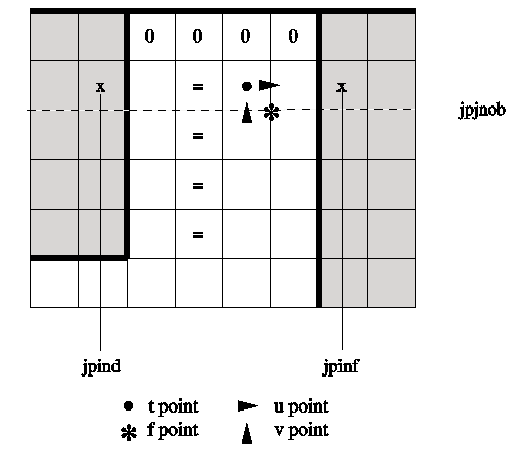
\includegraphics[width=0.70\textwidth]{./TexFiles/Figures/Fig_obc_north.pdf}
\caption{    \label{Fig_obc_north}
Localization of the North open boundary points.}
\end{center}     \end{figure}
%>>>>>>>>>>>>>>>>>>>>>>>>>>>>

Although not compulsory, it is highly recommended that the bathymetry in the 
vicinity of an open boundary follows the following rule: in the direction perpendicular 
to the open line, the water depth should be constant for 4 grid points. This is in 
order to ensure that the radiation condition, which involves model variables next 
to the boundary, is calculated in a consistent way. On Fig.\ref{Fig_obc_north} we 
indicate by an $=$ symbol, the points which should have the same depth. It means 
that at the 4 points near the boundary, the bathymetry is cylindrical \gmcomment{not sure 
why cylindrical}. The line behind the open $T$-line must be 0 in the bathymetry file 
(as shown on Fig.\ref{Fig_obc_north} for example).

%----------------------------------------------
\subsection{Boundary data}
\label{OBC_data}

It is necessary to provide information at the boundaries. The simplest case is 
when this information does not change in time and is equal to the initial conditions 
(namelist variable \np{nn\_obcdta}=0). This is the case for the standard configuration 
EEL5 with open boundaries. When (\np{nn\_obcdta}=1), open boundary information 
is read from netcdf files. For convenience the input files are supposed to be similar 
to the ''history'' NEMO output files, for dimension names and variable names. 
Open boundary arrays must be dimensioned according to the parameters of table~
\ref{Tab_obc_param}: for example, at the western boundary, arrays have a 
dimension of \jp{jpwf}-\jp{jpwd}+1 in the horizontal and \jp{jpk} in the vertical. 

When ocean observations are used to generate the boundary data (a hydrographic 
section for example, as in \citet{Treguier_al_JGR01}) it happens often that only the velocity 
normal to the boundary is known, which is the reason why the initial OBC code 
assumes that only $T$, $S$, and the normal velocity ($u$ or $v$) needs to be 
specified. As more and more global model solutions and ocean analysis products 
become available, it will be possible to provide information about all the variables 
(including the tangential velocity) so that the specification of four variables at each 
boundaries will become standard. For the sea surface height, one must distinguish 
between the filtered free surface case and the time-splitting or explicit treatment of 
the free surface.
 In the first case, it is assumed that the user does not wish to represent high 
 frequency motions such as tides. The boundary condition is thus one of zero 
 normal gradient of sea surface height at the open boundaries, following \citet{Marchesiello2001}. 
No information other than the total velocity needs to be provided at the open 
boundaries in that case. In the other two cases (time splitting or explicit free surface), 
the user must provide barotropic information (sea surface height and barotropic 
velocities) and the use of the Flather algorithm for barotropic variables is 
recommanded. However, this algorithm has not yet been fully tested and bugs 
remain in NEMO v2.3. Users should read the code carefully before using it. Finally, 
in the case of the rigid lid approximation the barotropic streamfunction must be 
provided, as documented in \citet{Treguier_al_JGR01}). This option is no longer 
recommended but remains in NEMO V2.3.

One frequently encountered case is when an open boundary domain is constructed 
from a global or larger scale NEMO configuration. Assuming the domain corresponds 
to indices $ib:ie$, $jb:je$ of the global domain, the bathymetry and forcing of the 
small domain can be created by using the following netcdf utility on the global files: 
ncks -F $-d\;x,ib,ie$ $-d\;y,jb,je$ (part of the nco series of utilities, 
see their \href{http://nco.sourceforge.net}{website}). 
The open boundary files can be constructed using ncks 
commands, following table~\ref{Tab_obc_ind}. 

%--------------------------------------------------TABLE--------------------------------------------------
\begin{table}[htbp]     \begin{center}      \begin{tabular}{|l|c|c|c|c|c|}
\hline
OBC  & Variable   & file name      & Index  & Start  & end  \\
West &  T,S       &   obcwest\_TS.nc &  $ib$+1     &   $jb$+1 &  $je-1$  \\
     &    U       &   obcwest\_U.nc  &  $ib$+1     &   $jb$+1 &  $je-1$  \\ 
     &    V       &   obcwest\_V.nc  &  $ib$+1     &   $jb$+1 &  $je-1$  \\       
\hline
East &  T,S       &   obceast\_TS.nc &  $ie$-1     &   $jb$+1 &  $je-1$  \\
     &    U       &   obceast\_U.nc  &  $ie$-2     &   $jb$+1 &  $je-1$  \\ 
     &    V       &   obceast\_V.nc  &  $ie$-1     &   $jb$+1 &  $je-1$  \\       
\hline         
South &  T,S      &   obcsouth\_TS.nc &  $jb$+1     &  $ib$+1 &  $ie-1$  \\
      &    U      &   obcsouth\_U.nc  &  $jb$+1     &  $ib$+1 &  $ie-1$  \\ 
      &    V      &   obcsouth\_V.nc  &  $jb$+1     &  $ib$+1 &  $ie-1$  \\    
\hline
North &  T,S      &   obcnorth\_TS.nc &  $je$-1     &  $ib$+1 &  $ie-1$  \\
      &    U      &   obcnorth\_U.nc  &  $je$-1     &  $ib$+1 &  $ie-1$  \\ 
      &    V      &   obcnorth\_V.nc  &  $je$-2     &  $ib$+1 &  $ie-1$  \\  
\hline
\end{tabular}     \end{center}
\caption{    \label{Tab_obc_ind}
Requirements for creating open boundary files from a global configuration, 
appropriate for the subdomain of indices $ib:ie$, $jb:je$. ``Index'' designates the 
$i$ or $j$ index along which the $u$ of $v$ boundary point is situated in the global 
configuration, starting and ending with the $j$ or $i$ indices indicated. 
For example, to generate file obcnorth\_V.nc, use the command ncks 
$-F$ $-d\;y,je-2$  $-d\;x,ib+1,ie-1$ } 
\end{table}
%-----------------------------------------------------------------------------------------------------------

It is assumed that the open boundary files contain the variables for the period of 
the model integration. If the boundary files contain one time frame, the boundary 
data is held fixed in time. If the files contain 12 values, it is assumed that the input 
is a climatology for a repeated annual cycle (corresponding to the case \np{ln\_obc\_clim} 
=true). The case of an arbitrary number of time frames is not yet implemented 
correctly; the user is required to write his own code in the module \mdl{obc\_dta} 
to deal with this situation. 

\subsection{Radiation algorithm}
\label{OBC_rad}

The art of open boundary management consists in applying a constraint strong 
enough that the inner domain "feels" the rest of the ocean, but weak enough
that perturbations are allowed to leave the domain with minimum false reflections 
of energy. The constraints are specified separately at each boundary as time 
scales for ''inflow'' and ''outflow'' as defined below. The time scales are set (in days) 
by namelist parameters such as \np{rn\_dpein}, \np{rn\_dpeob} for the eastern open 
boundary for example. When both time scales are zero for a given boundary 
($e.g.$ for the western boundary, \jp{lp\_obc\_west}=true, \np{rn\_dpwob}=0 and 
\np{rn\_dpwin}=0) this means that the boundary in question is a ''fixed '' boundary 
where the solution is set exactly by the boundary data. This is not recommended, 
except in combination with increased viscosity in a ''sponge'' layer next to the 
boundary in order to avoid spurious reflections.  


The radiation\/relaxation \gmcomment{the / doesnt seem to appear in the output} 
algorithm is applied when either relaxation time (for ''inflow'' or ''outflow'') is 
non-zero. It has been developed and tested in the SPEM model and its 
successor ROMS \citep{Barnier1996, Marchesiello2001}, which is an 
$s$-coordinate model on an Arakawa C-grid. Although the algorithm has 
been numerically successful in the CLIPPER Atlantic models, the physics 
do not work as expected \citep{Treguier_al_JGR01}. Users are invited to consider 
open boundary conditions (OBC hereafter) with some scepticism 
\citep{Durran2001, Blayo2005}.

The first part of the algorithm calculates a phase velocity to determine 
whether perturbations tend to propagate toward, or away from, the 
boundary. Let us consider a model variable $\phi$. 
The phase velocities ($C_{\phi x}$,$C_{\phi y}$) for the variable $\phi$, 
in the directions normal and tangential to the boundary are
\begin{equation} \label{Eq_obc_cphi}
C_{\phi x} = \frac{ -\phi_{t} }{ ( \phi_{x}^{2} + \phi_{y}^{2}) } \phi_{x} 
\;\;\;\;\; \;\;\; 
C_{\phi y} = \frac{ -\phi_{t} }{ ( \phi_{x}^{2} + \phi_{y}^{2}) } \phi_{y}. 
\end{equation}
Following \citet{Treguier_al_JGR01} and \citet{Marchesiello2001} we retain only 
the normal component of the velocity, $C_{\phi x}$, setting $C_{\phi y} =0$ 
(but unlike the original Orlanski radiation algorithm we retain $\phi_{y}$ in 
the expression for $C_{\phi x}$).  

The discrete form of (\ref{Eq_obc_cphi}), described by \citet{Barnier1998},
takes into account the two rows of grid points situated inside the domain 
next to the boundary, and the three previous time steps ($n$, $n-1$,
and $n-2$). The same equation can then be discretized at the boundary at
time steps $n-1$, $n$ and $n+1$ \gmcomment{since the original was three time-level} 
in order to extrapolate for the new boundary value $\phi^{n+1}$. 

In the open boundary algorithm as implemented in NEMO v2.3, the new boundary 
values are updated differently depending on the sign of $C_{\phi x}$. Let us take 
an eastern boundary as an example. The solution for variable $\phi$ at the 
boundary is given by a generalized wave equation with phase velocity $C_{\phi}$, 
with the addition of a relaxation term, as:
\begin{eqnarray}
\phi_{t} &  =  & -C_{\phi x} \phi_{x} + \frac{1}{\tau_{o}} (\phi_{c}-\phi) 
                        \;\;\; \;\;\; \;\;\; (C_{\phi x} > 0), \label{Eq_obc_rado} \\
\phi_{t} &  =  & \frac{1}{\tau_{i}} (\phi_{c}-\phi) 
\;\;\; \;\;\; \;\;\;\;\;\; (C_{\phi x} < 0), \label{Eq_obc_radi}
\end{eqnarray}
where $\phi_{c}$ is the estimate of $\phi$ at the boundary, provided as boundary 
data. Note that in (\ref{Eq_obc_rado}), $C_{\phi x}$ is bounded by the ratio 
$\delta x/\delta t$ for stability reasons. When $C_{\phi x}$ is eastward (outward 
propagation), the radiation condition (\ref{Eq_obc_rado}) is used. 
When  $C_{\phi x}$ is westward (inward propagation), (\ref{Eq_obc_radi}) is 
used with a strong relaxation to climatology (usually $\tau_{i}=\np{rn\_dpein}=$1~day).
Equation (\ref{Eq_obc_radi}) is solved with a Euler time-stepping scheme. As a 
consequence, setting $\tau_{i}$ smaller than, or equal to the time step is equivalent 
to a fixed boundary condition. A time scale of one day is usually a good compromise 
which guarantees that the inflow conditions remain close to climatology while ensuring 
numerical stability. 

In  the case of a western boundary located in the Eastern Atlantic, \citet{Penduff_al_JGR00} 
have been able to implement the radiation algorithm without any boundary data, 
using persistence from the previous time step instead. This solution has not worked 
in other cases \citep{Treguier_al_JGR01}, so that the use of boundary data is recommended. 
Even in the outflow condition (\ref{Eq_obc_rado}), we have found it desirable to 
maintain a weak relaxation to climatology. The time step is usually chosen so as to 
be larger than typical turbulent scales (of order 1000~days \gmcomment{or maybe seconds?}).

The radiation condition is applied to the model variables: temperature, salinity, 
tangential and normal velocities. For normal and tangential velocities, $u$ and $v$, 
radiation is applied with phase velocities calculated from $u$ and $v$ respectively.  
For the radiation of tracers, we use the phase velocity calculated from the tangential 
velocity in order to avoid calculating too many independent radiation velocities and 
because tangential velocities and tracers have the same position along the boundary 
on a C-grid.  

\subsection{Domain decomposition (\key{mpp\_mpi})}
\label{OBC_mpp}
When \key{mpp\_mpi} is active in the code, the computational domain is divided 
into rectangles that are attributed each to a different processor. The open boundary 
code is ``mpp-compatible'' up to a certain point. The radiation algorithm will not 
work if there is an mpp subdomain boundary parallel to the open boundary at the 
index of the boundary, or the grid point after (outside), or three grid points before 
(inside). On the other hand, there is no problem if an mpp subdomain boundary 
cuts the open boundary perpendicularly. These geometrical limitations must be 
checked for by the user (there is no safeguard in the code).  
The general principle for the open boundary mpp code is that loops over the open 
boundaries {not sure what this means} are performed on local indices (nie0, 
nie1, nje0, nje1 for an eastern boundary for instance) that are initialized in module 
\mdl{obc\_ini}. Those indices have relevant values on the processors that contain 
a segment of an open boundary. For processors that do not include an open 
boundary segment, the indices are such that the calculations within the loops are 
not performed.
\gmcomment{I dont understand most of the last few sentences}
 
Arrays of climatological data that are read from files are seen by all processors 
and have the same dimensions for all (for instance, for the eastern boundary, 
uedta(jpjglo,jpk,2)). On the other hand, the arrays for the calculation of radiation 
are local to each processor (uebnd(jpj,jpk,3,3) for instance).  This allowed the 
CLIPPER model for example, to save on memory where the eastern boundary 
crossed 8 processors so that \jp{jpj} was much smaller than (\jp{jpjef}-\jp{jpjed}+1). 

\subsection{Volume conservation}
\label{OBC_vol}

It is necessary to control the volume inside a domain when using open boundaries. 
With fixed boundaries, it is enough to ensure that the total inflow/outflow has 
reasonable values (either zero or a value compatible with an observed volume 
balance). When using radiative boundary conditions it is necessary to have a 
volume constraint because each open boundary works independently from the 
others. The methodology used to control this volume is identical to the one 
coded in the ROMS model \citep{Marchesiello2001}.


%---------------------------------------- EXTRAS
\colorbox{yellow}{Explain obc\_vol{\ldots}}

\colorbox{yellow}{OBC algorithm for update, OBC restart, list of routines where obc key appears{\ldots}}

\colorbox{yellow}{OBC rigid lid? {\ldots}}

% ====================================================================
% Unstructured open boundaries BDY 
% ====================================================================
\section{Unstructured Open Boundary Conditions (\key{bdy}) (BDY)}
\label{LBC_bdy}

%-----------------------------------------nambdy--------------------------------------------
\namdisplay{nambdy} 
%-----------------------------------------------------------------------------------------------
%-----------------------------------------nambdy_index--------------------------------------------
\namdisplay{nambdy_index} 
%-----------------------------------------------------------------------------------------------
%-----------------------------------------nambdy_dta--------------------------------------------
\namdisplay{nambdy_dta} 
%-----------------------------------------------------------------------------------------------
%-----------------------------------------nambdy_dta--------------------------------------------
\namdisplay{nambdy_dta2} 
%-----------------------------------------------------------------------------------------------

Options are defined through the \ngn{nambdy} \ngn{nambdy\_index} 
\ngn{nambdy\_dta} \ngn{nambdy\_dta2} namelist variables.
The BDY module is an alternative implementation of open boundary
conditions for regional configurations. It implements the Flow
Relaxation Scheme algorithm for temperature, salinity, velocities and
ice fields, and the Flather radiation condition for the depth-mean
transports. The specification of the location of the open boundary is
completely flexible and allows for example the open boundary to follow
an isobath or other irregular contour. 

The BDY module was modelled on the OBC module and shares many features
and a similar coding structure \citep{Chanut2005}.

The BDY module is completely rewritten at NEMO 3.4 and there is a new
set of namelists. Boundary data files used with earlier versions of
NEMO may need to be re-ordered to work with this version. See the
section on the Input Boundary Data Files for details.

%----------------------------------------------
\subsection{The namelists}
\label{BDY_namelist}

It is possible to define more than one boundary ``set'' and apply
different boundary conditions to each set. The number of boundary
sets is defined by \np{nb\_bdy}.  Each boundary set may be defined
as a set of straight line segments in a namelist
(\np{ln\_coords\_file}=.false.) or read in from a file
(\np{ln\_coords\_file}=.true.). If the set is defined in a namelist,
then the namelists nambdy\_index must be included separately, one for
each set. If the set is defined by a file, then a
``coordinates.bdy.nc'' file must be provided. The coordinates.bdy file
is analagous to the usual NEMO ``coordinates.nc'' file. In the example
above, there are two boundary sets, the first of which is defined via
a file and the second is defined in a namelist. For more details of
the definition of the boundary geometry see section
\ref{BDY_geometry}.

For each boundary set a boundary
condition has to be chosen for the barotropic solution (``u2d'':
sea-surface height and barotropic velocities), for the baroclinic
velocities (``u3d''), and for the active tracers\footnote{The BDY
  module does not deal with passive tracers at this version}
(``tra''). For each set of variables there is a choice of algorithm
and a choice for the data, eg. for the active tracers the algorithm is
set by \np{nn\_tra} and the choice of data is set by
\np{nn\_tra\_dta}. 

The choice of algorithm is currently as follows:

\mbox{}

\begin{itemize}
\item[0.] No boundary condition applied. So the solution will ``see''
  the land points around the edge of the edge of the domain.
\item[1.] Flow Relaxation Scheme (FRS) available for all variables. 
\item[2.] Flather radiation scheme for the barotropic variables. The
  Flather scheme is not compatible with the filtered free surface
  ({\it dynspg\_ts}). 
\end{itemize}

\mbox{}

The main choice for the boundary data is
to use initial conditions as boundary data (\np{nn\_tra\_dta}=0) or to
use external data from a file (\np{nn\_tra\_dta}=1). For the
barotropic solution there is also the option to use tidal
harmonic forcing either by itself or in addition to other external
data. 

If external boundary data is required then the nambdy\_dta namelist
must be defined. One nambdy\_dta namelist is required for each boundary
set in the order in which the boundary sets are defined in nambdy. In
the example given, two boundary sets have been defined and so there
are two nambdy\_dta namelists. The boundary data is read in using the
fldread module, so the nambdy\_dta namelist is in the format required
for fldread. For each variable required, the filename, the frequency
of the files and the frequency of the data in the files is given. Also
whether or not time-interpolation is required and whether the data is
climatological (time-cyclic) data. Note that on-the-fly spatial
interpolation of boundary data is not available at this version. 

In the example namelists given, two boundary sets are defined. The
first set is defined via a file and applies FRS conditions to
temperature and salinity and Flather conditions to the barotropic
variables. External data is provided in daily files (from a
large-scale model). Tidal harmonic forcing is also used. The second
set is defined in a namelist. FRS conditions are applied on
temperature and salinity and climatological data is read from external
files. 

%----------------------------------------------
\subsection{The Flow Relaxation Scheme}
\label{BDY_FRS_scheme}

The Flow Relaxation Scheme (FRS) \citep{Davies_QJRMS76,Engerdahl_Tel95},
applies a simple relaxation of the model fields to
externally-specified values over a zone next to the edge of the model
domain. Given a model prognostic variable $\Phi$ 
\begin{equation}  \label{Eq_bdy_frs1}
\Phi(d) = \alpha(d)\Phi_{e}(d) + (1-\alpha(d))\Phi_{m}(d)\;\;\;\;\; d=1,N
\end{equation}
where $\Phi_{m}$ is the model solution and $\Phi_{e}$ is the specified
external field, $d$ gives the discrete distance from the model
boundary  and $\alpha$ is a parameter that varies from $1$ at $d=1$ to
a small value at $d=N$. It can be shown that this scheme is equivalent
to adding a relaxation term to the prognostic equation for $\Phi$ of
the form:
\begin{equation}  \label{Eq_bdy_frs2}
-\frac{1}{\tau}\left(\Phi - \Phi_{e}\right)
\end{equation}
where the relaxation time scale $\tau$ is given by a function of
$\alpha$ and the model time step $\Delta t$:
\begin{equation}  \label{Eq_bdy_frs3}
\tau = \frac{1-\alpha}{\alpha}  \,\rdt
\end{equation}
Thus the model solution is completely prescribed by the external
conditions at the edge of the model domain and is relaxed towards the
external conditions over the rest of the FRS zone. The application of
a relaxation zone helps to prevent spurious reflection of outgoing
signals from the model boundary. 

The function $\alpha$ is specified as a $tanh$ function:
\begin{equation}  \label{Eq_bdy_frs4}
\alpha(d) = 1 - \tanh\left(\frac{d-1}{2}\right),       \quad d=1,N
\end{equation}
The width of the FRS zone is specified in the namelist as 
\np{nn\_rimwidth}. This is typically set to a value between 8 and 10. 

%----------------------------------------------
\subsection{The Flather radiation scheme}
\label{BDY_flather_scheme}

The \citet{Flather_JPO94} scheme is a radiation condition on the normal, depth-mean
transport across the open boundary. It takes the form
\begin{equation}  \label{Eq_bdy_fla1}
U = U_{e} + \frac{c}{h}\left(\eta - \eta_{e}\right),
\end{equation}
where $U$ is the depth-mean velocity normal to the boundary and $\eta$
is the sea surface height, both from the model. The subscript $e$
indicates the same fields from external sources. The speed of external
gravity waves is given by $c = \sqrt{gh}$, and $h$ is the depth of the
water column. The depth-mean normal velocity along the edge of the
model domain is set equal to the
external depth-mean normal velocity, plus a correction term that
allows gravity waves generated internally to exit the model boundary.
Note that the sea-surface height gradient in \eqref{Eq_bdy_fla1}
is a spatial gradient across the model boundary, so that $\eta_{e}$ is
defined on the $T$ points with $nbr=1$ and $\eta$ is defined on the
$T$ points with $nbr=2$. $U$ and $U_{e}$ are defined on the $U$ or
$V$ points with $nbr=1$, $i.e.$ between the two $T$ grid points.

%----------------------------------------------
\subsection{Boundary geometry}
\label{BDY_geometry}

Each open boundary set is defined as a list of points. The information
is stored in the arrays $nbi$, $nbj$, and $nbr$ in the $idx\_bdy$
structure.  The $nbi$ and $nbj$ arrays
define the local $(i,j)$ indices of each point in the boundary zone
and the $nbr$ array defines the discrete distance from the boundary
with $nbr=1$ meaning that the point is next to the edge of the
model domain and $nbr>1$ showing that the point is increasingly
further away from the edge of the model domain. A set of $nbi$, $nbj$,
and $nbr$ arrays is defined for each of the $T$, $U$ and $V$
grids. Figure \ref{Fig_LBC_bdy_geom} shows an example of an irregular
boundary. 

The boundary geometry for each set may be defined in a namelist
nambdy\_index or by reading in a ``coordinates.bdy.nc'' file. The
nambdy\_index namelist defines a series of straight-line segments for
north, east, south and west boundaries. For the northern boundary,
\np{nbdysegn} gives the number of segments, \np{jpjnob} gives the $j$
index for each segment and \np{jpindt} and \np{jpinft} give the start
and end $i$ indices for each segment with similar for the other
boundaries. These segments define a list of $T$ grid points along the
outermost row of the boundary ($nbr\,=\, 1$). The code deduces the $U$ and
$V$ points and also the points for $nbr\,>\, 1$ if
$nn\_rimwidth\,>\,1$.

The boundary geometry may also be defined from a
``coordinates.bdy.nc'' file. Figure \ref{Fig_LBC_nc_header}
gives an example of the header information from such a file. The file
should contain the index arrays for each of the $T$, $U$ and $V$
grids. The arrays must be in order of increasing $nbr$. Note that the
$nbi$, $nbj$ values in the file are global values and are converted to
local values in the code. Typically this file will be used to generate
external boundary data via interpolation and so will also contain the
latitudes and longitudes of each point as shown. However, this is not
necessary to run the model. 

For some choices of irregular boundary the model domain may contain
areas of ocean which are not part of the computational domain. For
example if an open boundary is defined along an isobath, say at the
shelf break, then the areas of ocean outside of this boundary will
need to be masked out. This can be done by reading a mask file defined
as \np{cn\_mask\_file} in the nam\_bdy namelist. Only one mask file is
used even if multiple boundary sets are defined.

%>>>>>>>>>>>>>>>>>>>>>>>>>>>>
\begin{figure}[!t]      \begin{center}
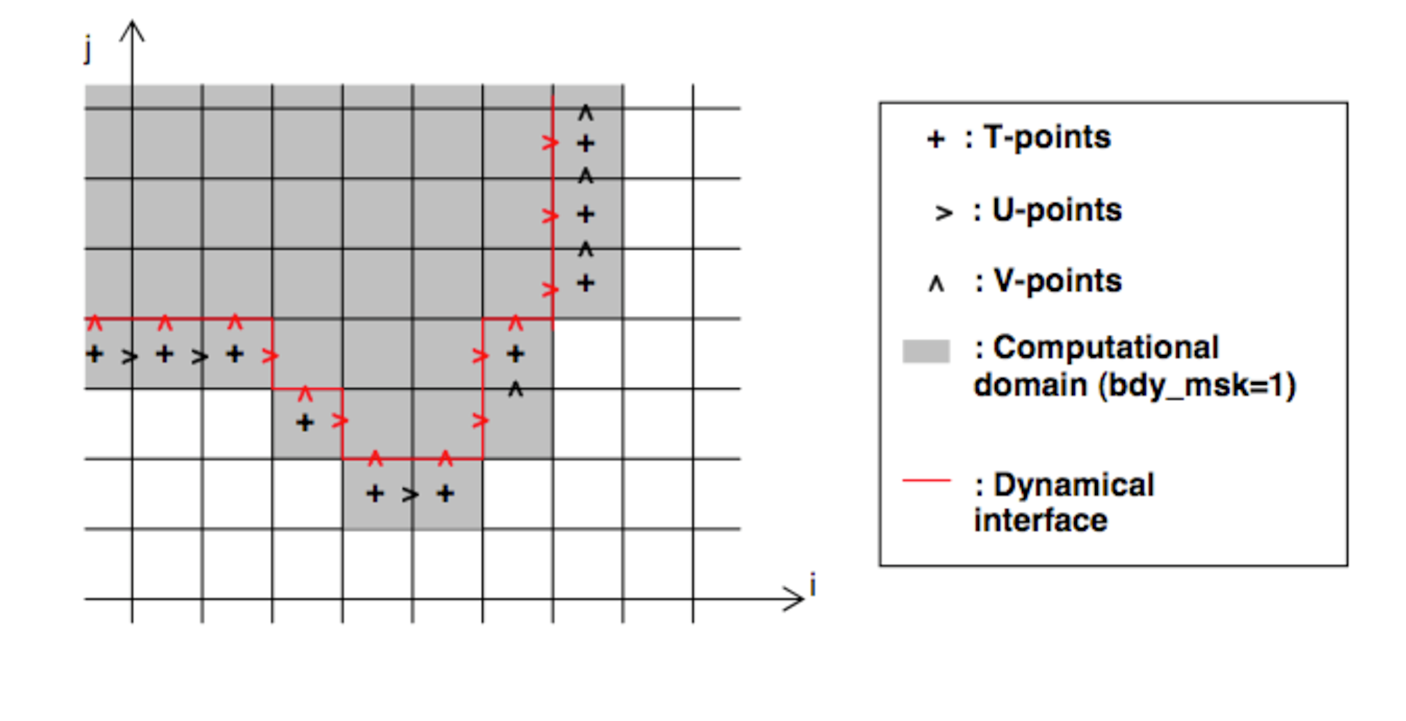
\includegraphics[width=1.0\textwidth]{./TexFiles/Figures/Fig_LBC_bdy_geom.pdf}
\caption {      \label{Fig_LBC_bdy_geom}
Example of geometry of unstructured open boundary}
\end{center}   \end{figure}
%>>>>>>>>>>>>>>>>>>>>>>>>>>>>

%----------------------------------------------
\subsection{Input boundary data files}
\label{BDY_data}

The data files contain the data arrays
in the order in which the points are defined in the $nbi$ and $nbj$
arrays. The data arrays are dimensioned on: a time dimension;
$xb$ which is the index of the boundary data point in the horizontal;
and $yb$ which is a degenerate dimension of 1 to enable the file to be
read by the standard NEMO I/O routines. The 3D fields also have a
depth dimension. 

At Version 3.4 there are new restrictions on the order in which the
boundary points are defined (and therefore restrictions on the order
of the data in the file). In particular:

\mbox{}

\begin{enumerate}
\item The data points must be in order of increasing $nbr$, ie. all
  the $nbr=1$ points, then all the $nbr=2$ points etc.
\item All the data for a particular boundary set must be in the same
  order. (Prior to 3.4 it was possible to define barotropic data in a
  different order to the data for tracers and baroclinic velocities). 
\end{enumerate}

\mbox{}

These restrictions mean that data files used with previous versions of
the model may not work with version 3.4. A fortran utility
{\it bdy\_reorder} exists in the TOOLS directory which will re-order the
data in old BDY data files. 

%>>>>>>>>>>>>>>>>>>>>>>>>>>>>
\begin{figure}[!t]     \begin{center}
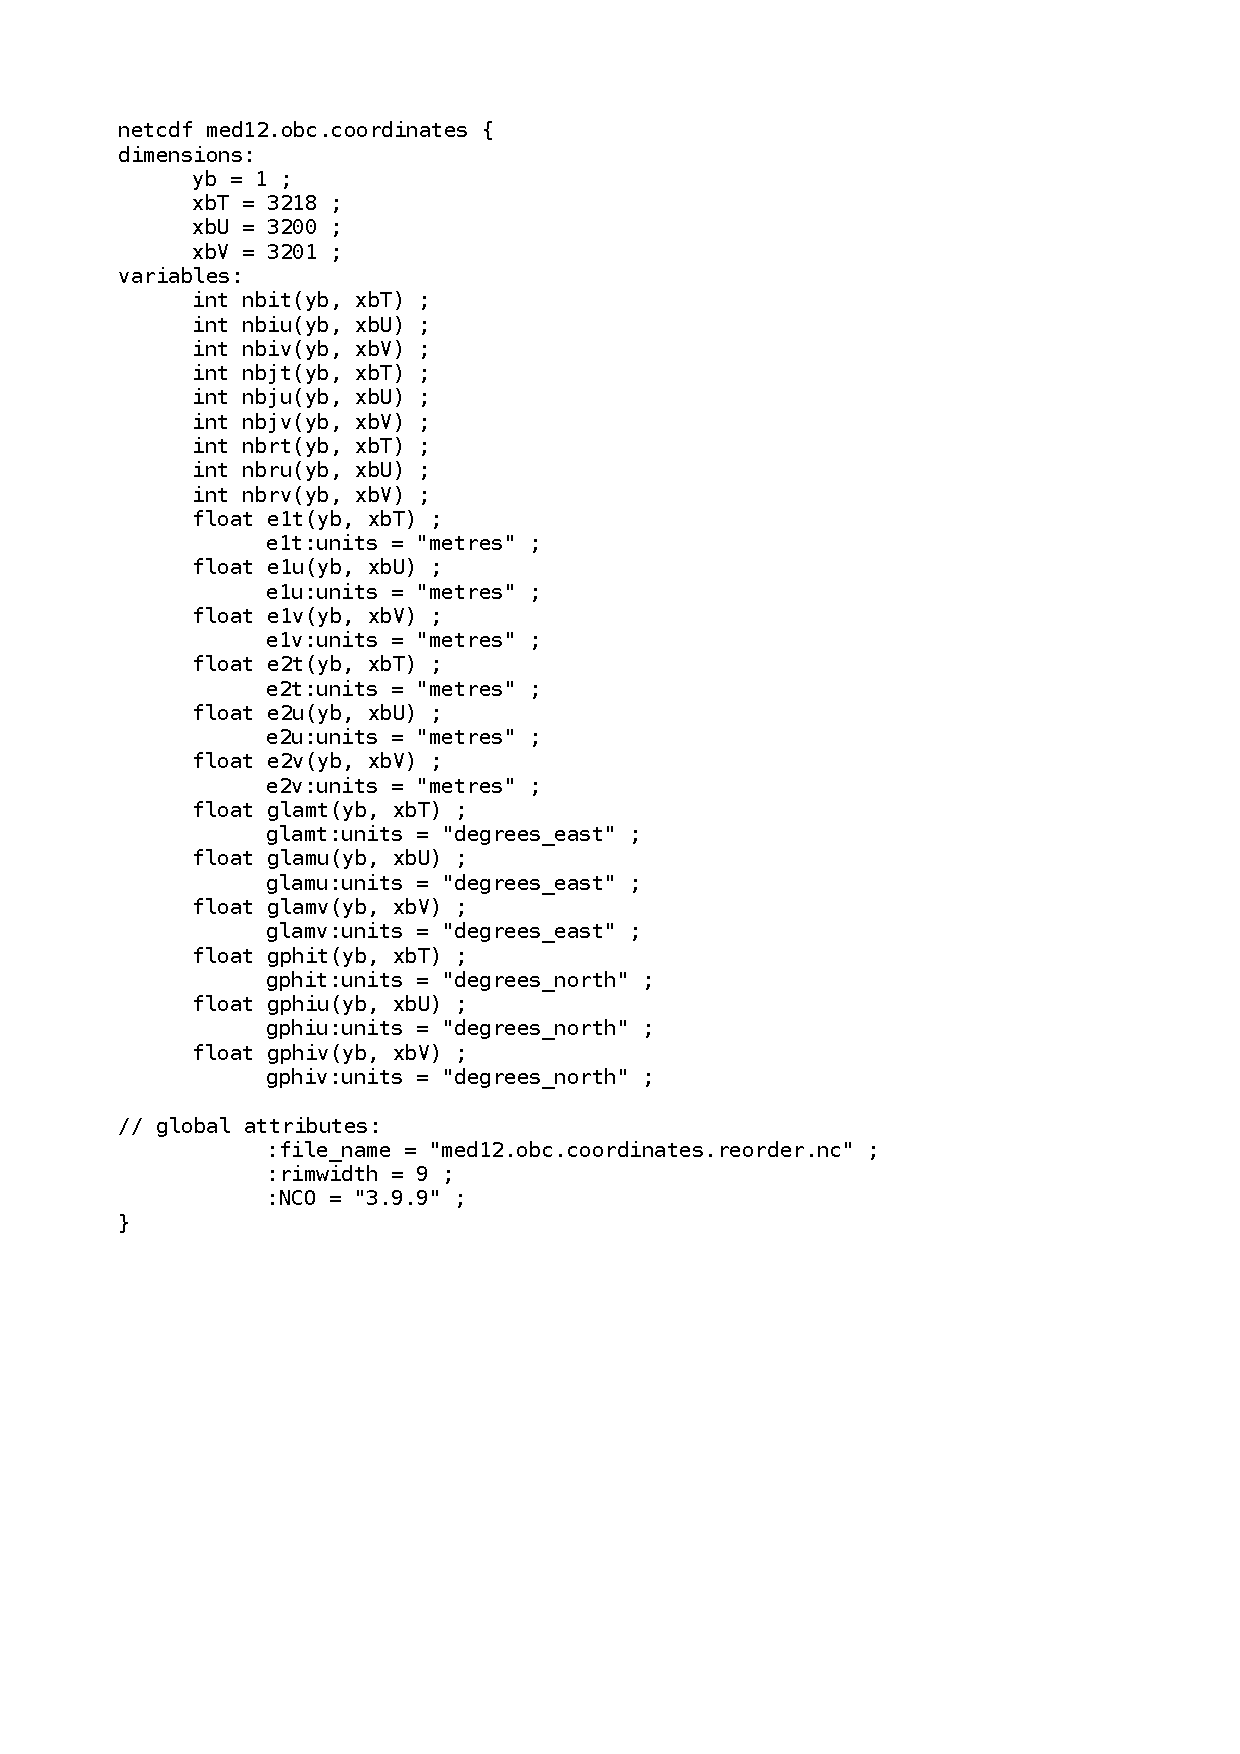
\includegraphics[width=1.0\textwidth]{./TexFiles/Figures/Fig_LBC_nc_header.pdf}
\caption {     \label{Fig_LBC_nc_header} 
Example of the header for a coordinates.bdy.nc file}
\end{center}   \end{figure}
%>>>>>>>>>>>>>>>>>>>>>>>>>>>>

%----------------------------------------------
\subsection{Volume correction}
\label{BDY_vol_corr}

There is an option to force the total volume in the regional model to be constant, 
similar to the option in the OBC module. This is controlled  by the \np{nn\_volctl} 
parameter in the namelist. A value of \np{nn\_volctl}~=~0 indicates that this option is not used. 
If  \np{nn\_volctl}~=~1 then a correction is applied to the normal velocities 
around the boundary at each timestep to ensure that the integrated volume flow 
through the boundary is zero. If \np{nn\_volctl}~=~2 then the calculation of 
the volume change on the timestep includes the change due to the freshwater 
flux across the surface and the correction velocity corrects for this as well.

If more than one boundary set is used then volume correction is
applied to all boundaries at once.

\newpage
%----------------------------------------------
\subsection{Tidal harmonic forcing}
\label{BDY_tides}

%-----------------------------------------nambdy_tide--------------------------------------------
\namdisplay{nambdy_tide} 
%-----------------------------------------------------------------------------------------------

Options are defined through the  \ngn{nambdy\_tide} namelist variables.
 To be written....




			% Lateral Boundary Conditions


% ================================================================
% Chapter � Lateral Ocean Physics (LDF)
% ================================================================
\chapter{Lateral Ocean Physics (LDF)}
\label{LDF}
\minitoc


\newpage
$\ $\newline    % force a new ligne


The lateral physics terms in the momentum and tracer equations have been 
described in \S\ref{PE_zdf} and their discrete formulation in \S\ref{TRA_ldf} 
and \S\ref{DYN_ldf}). In this section we further discuss each lateral physics option. 
Choosing one lateral physics scheme means for the user defining, (1) the space 
and time variations of the eddy coefficients ; (2) the direction along which the 
lateral diffusive fluxes are evaluated (model level, geopotential or isopycnal 
surfaces); and (3) the type of operator used (harmonic, or biharmonic operators, 
and for tracers only, eddy induced advection on tracers). These three aspects 
of the lateral diffusion are set through namelist parameters and CPP keys 
(see the \textit{\ngn{nam\_traldf}} and \textit{\ngn{nam\_dynldf}} below). Note
that this chapter describes the default implementation of iso-neutral
tracer mixing, and Griffies's implementation, which is used if
\np{traldf\_grif}=true, is described in Appdx\ref{sec:triad}

%-----------------------------------nam_traldf - nam_dynldf--------------------------------------------
\namdisplay{namtra_ldf} 
\namdisplay{namdyn_ldf} 
%--------------------------------------------------------------------------------------------------------------


% ================================================================
% Lateral Mixing Coefficients
% ================================================================
\section [Lateral Mixing Coefficient (\textit{ldftra}, \textit{ldfdyn})] 
		  {Lateral Mixing Coefficient (\mdl{ldftra}, \mdl{ldfdyn}) }
\label{LDF_coef}


Introducing a space variation in the lateral eddy mixing coefficients changes 
the model core memory requirement, adding up to four extra three-dimensional 
arrays for the geopotential or isopycnal second order operator applied to 
momentum. Six CPP keys control the space variation of eddy coefficients: 
three for momentum and three for tracer. The three choices allow: 
a space variation in the three space directions (\key{traldf\_c3d},  \key{dynldf\_c3d}), 
in the horizontal plane (\key{traldf\_c2d},  \key{dynldf\_c2d}), 
or in the vertical only (\key{traldf\_c1d},  \key{dynldf\_c1d}). 
The default option is a constant value over the whole ocean on both momentum and tracers. 
   
The number of additional arrays that have to be defined and the gridpoint 
position at which they are defined depend on both the space variation chosen 
and the type of operator used. The resulting eddy viscosity and diffusivity 
coefficients can be a function of more than one variable. Changes in the 
computer code when switching from one option to another have been 
minimized by introducing the eddy coefficients as statement functions
(include file \hf{ldftra\_substitute} and \hf{ldfdyn\_substitute}). The functions 
are replaced by their actual meaning during the preprocessing step (CPP). 
The specification of the space variation of the coefficient is made in 
\mdl{ldftra} and \mdl{ldfdyn}, or more precisely in include files 
\textit{traldf\_cNd.h90} and \textit{dynldf\_cNd.h90}, with N=1, 2 or 3. 
The user can modify these include files as he/she wishes. The way the 
mixing coefficient are set in the reference version can be briefly described 
as follows:

\subsubsection{Constant Mixing Coefficients (default option)}
When none of the \textbf{key\_dynldf\_...} and \textbf{key\_traldf\_...} keys are 
defined, a constant value is used over the whole ocean for momentum and 
tracers, which is specified through the \np{rn\_ahm0} and \np{rn\_aht0} namelist 
parameters.

\subsubsection{Vertically varying Mixing Coefficients (\key{traldf\_c1d} and \key{dynldf\_c1d})} 
The 1D option is only available when using the $z$-coordinate with full step. 
Indeed in all the other types of vertical coordinate, the depth is a 3D function 
of (\textbf{i},\textbf{j},\textbf{k}) and therefore, introducing depth-dependent 
mixing coefficients will require 3D arrays. In the 1D option, a hyperbolic variation 
of the lateral mixing coefficient is introduced in which the surface value is 
\np{rn\_aht0} (\np{rn\_ahm0}), the bottom value is 1/4 of the surface value, 
and the transition takes place around z=300~m with a width of 300~m 
($i.e.$ both the depth and the width of the inflection point are set to 300~m). 
This profile is hard coded in file \hf{traldf\_c1d}, but can be easily modified by users.

\subsubsection{Horizontally Varying Mixing Coefficients (\key{traldf\_c2d} and \key{dynldf\_c2d})}
By default the horizontal variation of the eddy coefficient depends on the local mesh 
size and the type of operator used:
\begin{equation} \label{Eq_title}
  A_l = \left\{     
   \begin{aligned}
         & \frac{\max(e_1,e_2)}{e_{max}} A_o^l  			& \text{for laplacian operator } \\
         & \frac{\max(e_1,e_2)^{3}}{e_{max}^{3}} A_o^l          & \text{for bilaplacian operator } 
   \end{aligned}    \right.
\end{equation}
where $e_{max}$ is the maximum of $e_1$ and $e_2$ taken over the whole masked 
ocean domain, and $A_o^l$ is the \np{rn\_ahm0} (momentum) or \np{rn\_aht0} (tracer) 
namelist parameter. This variation is intended to reflect the lesser need for subgrid 
scale eddy mixing where the grid size is smaller in the domain. It was introduced in 
the context of the DYNAMO modelling project \citep{Willebrand_al_PO01}. 
Note that such a grid scale dependance of mixing coefficients significantly increase 
the range of stability of model configurations presenting large changes in grid pacing 
such as global ocean models. Indeed, in such a case, a constant mixing coefficient 
can lead to a blow up of the model due to large coefficient compare to the smallest 
grid size (see \S\ref{STP_forward_imp}), especially when using a bilaplacian operator.

Other formulations can be introduced by the user for a given configuration. 
For example, in the ORCA2 global ocean model (see Configurations), the laplacian 
viscosity operator uses \np{rn\_ahm0}~= 4.10$^4$ m$^2$/s poleward of 20$^{\circ}$ 
north and south and decreases linearly to \np{rn\_aht0}~= 2.10$^3$ m$^2$/s 
at the equator \citep{Madec_al_JPO96, Delecluse_Madec_Bk00}. This modification 
can be found in routine \rou{ldf\_dyn\_c2d\_orca} defined in \mdl{ldfdyn\_c2d}. 
Similar modified horizontal variations can be found with the Antarctic or Arctic 
sub-domain options of ORCA2 and ORCA05 (see \&namcfg namelist).

\subsubsection{Space Varying Mixing Coefficients (\key{traldf\_c3d} and \key{dynldf\_c3d})}

The 3D space variation of the mixing coefficient is simply the combination of the 
1D and 2D cases, $i.e.$ a hyperbolic tangent variation with depth associated with 
a grid size dependence of the magnitude of the coefficient. 

\subsubsection{Space and Time Varying Mixing Coefficients}

There is no default specification of space and time varying mixing coefficient. 
The only case available is specific to the ORCA2 and ORCA05 global ocean 
configurations. It provides only a tracer 
mixing coefficient for eddy induced velocity (ORCA2) or both iso-neutral and 
eddy induced velocity (ORCA05) that depends on the local growth rate of 
baroclinic instability. This specification is actually used when an ORCA key 
and both \key{traldf\_eiv} and \key{traldf\_c2d} are defined.

$\ $\newline    % force a new ligne

The following points are relevant when the eddy coefficient varies spatially:

(1) the momentum diffusion operator acting along model level surfaces is 
written in terms of curl and divergent components of the horizontal current 
(see \S\ref{PE_ldf}). Although the eddy coefficient could be set to different values 
in these two terms, this option is not currently available. 

(2) with an horizontally varying viscosity, the quadratic integral constraints 
on enstrophy and on the square of the horizontal divergence for operators 
acting along model-surfaces are no longer satisfied 
(Appendix~\ref{Apdx_dynldf_properties}).

(3) for isopycnal diffusion on momentum or tracers, an additional purely 
horizontal background diffusion with uniform coefficient can be added by 
setting a non zero value of \np{rn\_ahmb0} or \np{rn\_ahtb0}, a background horizontal 
eddy viscosity or diffusivity coefficient (namelist parameters whose default 
values are $0$). However, the technique used to compute the isopycnal 
slopes is intended to get rid of such a background diffusion, since it introduces 
spurious diapycnal diffusion (see {\S\ref{LDF_slp}).

(4) when an eddy induced advection term is used (\key{traldf\_eiv}), $A^{eiv}$, 
the eddy induced coefficient has to be defined. Its space variations are controlled 
by the same CPP variable as for the eddy diffusivity coefficient ($i.e.$ 
\textbf{key\_traldf\_cNd}). 

(5) the eddy coefficient associated with a biharmonic operator must be set to a \emph{negative} value.

(6) it is possible to use both the laplacian and biharmonic operators concurrently.

(7) it is possible to run without explicit lateral diffusion on momentum (\np{ln\_dynldf\_lap} = 
\np{ln\_dynldf\_bilap} = false). This is recommended when using the UBS advection 
scheme on momentum (\np{ln\_dynadv\_ubs} = true, see \ref{DYN_adv_ubs}) 
and can be useful for testing purposes.

% ================================================================
% Direction of lateral Mixing
% ================================================================
\section  [Direction of Lateral Mixing (\textit{ldfslp})]
		{Direction of Lateral Mixing (\mdl{ldfslp})}
\label{LDF_slp}

%%%
\gmcomment{  we should emphasize here that the implementation is a rather old one. 
Better work can be achieved by using \citet{Griffies_al_JPO98, Griffies_Bk04} iso-neutral scheme. }

A direction for lateral mixing has to be defined when the desired operator does 
not act along the model levels. This occurs when $(a)$ horizontal mixing is 
required on tracer or momentum (\np{ln\_traldf\_hor} or \np{ln\_dynldf\_hor}) 
in $s$- or mixed $s$-$z$- coordinates, and $(b)$ isoneutral mixing is required 
whatever the vertical coordinate is. This direction of mixing is defined by its 
slopes in the \textbf{i}- and \textbf{j}-directions at the face of the cell of the 
quantity to be diffused. For a tracer, this leads to the following four slopes : 
$r_{1u}$, $r_{1w}$, $r_{2v}$, $r_{2w}$ (see \eqref{Eq_tra_ldf_iso}), while 
for momentum the slopes are  $r_{1t}$, $r_{1uw}$, $r_{2f}$, $r_{2uw}$ for 
$u$ and  $r_{1f}$, $r_{1vw}$, $r_{2t}$, $r_{2vw}$ for $v$. 

%gm% add here afigure of the slope in i-direction

\subsection{slopes for tracer geopotential mixing in the $s$-coordinate}

In $s$-coordinates, geopotential mixing ($i.e.$ horizontal mixing) $r_1$ and 
$r_2$ are the slopes between the geopotential and computational surfaces. 
Their discrete formulation is found by locally solving \eqref{Eq_tra_ldf_iso} 
when the diffusive fluxes in the three directions are set to zero and $T$ is 
assumed to be horizontally uniform, $i.e.$ a linear function of $z_T$, the 
depth of a $T$-point. 
%gm { Steven : My version is obviously wrong since I'm left with an arbitrary constant which is the local vertical temperature gradient}

\begin{equation} \label{Eq_ldfslp_geo}
\begin{aligned}
 r_{1u} &= \frac{e_{3u}}{ \left( e_{1u}\;\overline{\overline{e_{3w}}}^{\,i+1/2,\,k} \right)}
 			  \;\delta_{i+1/2}[z_t] 
 		&\approx \frac{1}{e_{1u}}\; \delta_{i+1/2}[z_t] 
\\
 r_{2v} &= \frac{e_{3v}}{\left( e_{2v}\;\overline{\overline{e_{3w}}}^{\,j+1/2,\,k} \right)} 
 			  \;\delta_{j+1/2} [z_t] 
		&\approx \frac{1}{e_{2v}}\; \delta_{j+1/2}[z_t] 
\\
 r_{1w} &= \frac{1}{e_{1w}}\;\overline{\overline{\delta_{i+1/2}[z_t]}}^{\,i,\,k+1/2}
 		&\approx \frac{1}{e_{1w}}\; \delta_{i+1/2}[z_{uw}] 
 \\
 r_{2w} &= \frac{1}{e_{2w}}\;\overline{\overline{\delta_{j+1/2}[z_t]}}^{\,j,\,k+1/2}
		&\approx \frac{1}{e_{2w}}\; \delta_{j+1/2}[z_{vw}] 
 \\
\end{aligned}
\end{equation}

%gm%  caution I'm not sure the simplification was a good idea! 

These slopes are computed once in \rou{ldfslp\_init} when \np{ln\_sco}=True, 
and either \np{ln\_traldf\_hor}=True or \np{ln\_dynldf\_hor}=True. 

\subsection{Slopes for tracer iso-neutral mixing}\label{LDF_slp_iso}
In iso-neutral mixing  $r_1$ and $r_2$ are the slopes between the iso-neutral 
and computational surfaces. Their formulation does not depend on the vertical 
coordinate used. Their discrete formulation is found using the fact that the 
diffusive fluxes of locally referenced potential density ($i.e.$ $in situ$ density) 
vanish. So, substituting $T$ by $\rho$ in \eqref{Eq_tra_ldf_iso} and setting the 
diffusive fluxes in the three directions to zero leads to the following definition for 
the neutral slopes:

\begin{equation} \label{Eq_ldfslp_iso}
\begin{split}
 r_{1u} &= \frac{e_{3u}}{e_{1u}}\; \frac{\delta_{i+1/2}[\rho]}
 								{\overline{\overline{\delta_{k+1/2}[\rho]}}^{\,i+1/2,\,k}}
\\
 r_{2v} &= \frac{e_{3v}}{e_{2v}}\; \frac{\delta_{j+1/2}\left[\rho \right]}
 								{\overline{\overline{\delta_{k+1/2}[\rho]}}^{\,j+1/2,\,k}}
\\
 r_{1w} &= \frac{e_{3w}}{e_{1w}}\; 
 			\frac{\overline{\overline{\delta_{i+1/2}[\rho]}}^{\,i,\,k+1/2}}
				 {\delta_{k+1/2}[\rho]}
\\
 r_{2w} &= \frac{e_{3w}}{e_{2w}}\; 
 			\frac{\overline{\overline{\delta_{j+1/2}[\rho]}}^{\,j,\,k+1/2}}
				 {\delta_{k+1/2}[\rho]}
\\
\end{split}
\end{equation}

%gm% rewrite this as the explanation is not very clear !!!
%In practice, \eqref{Eq_ldfslp_iso} is of little help in evaluating the neutral surface slopes. Indeed, for an unsimplified equation of state, the density has a strong dependancy on pressure (here approximated as the depth), therefore applying \eqref{Eq_ldfslp_iso} using the $in situ$ density, $\rho$, computed at T-points leads to a flattening of slopes as the depth increases. This is due to the strong increase of the $in situ$ density with depth. 

%By definition, neutral surfaces are tangent to the local $in situ$ density \citep{McDougall1987}, therefore in \eqref{Eq_ldfslp_iso}, all the derivatives have to be evaluated at the same local pressure (which in decibars is approximated by the depth in meters).

%In the $z$-coordinate, the derivative of the  \eqref{Eq_ldfslp_iso} numerator is evaluated at the same depth \nocite{as what?} ($T$-level, which is the same as the $u$- and $v$-levels), so  the $in situ$ density can be used for its evaluation. 

As the mixing is performed along neutral surfaces, the gradient of $\rho$ in 
\eqref{Eq_ldfslp_iso} has to be evaluated at the same local pressure (which, 
in decibars, is approximated by the depth in meters in the model). Therefore 
\eqref{Eq_ldfslp_iso} cannot be used as such, but further transformation is 
needed depending on the vertical coordinate used:

\begin{description}

\item[$z$-coordinate with full step : ] in \eqref{Eq_ldfslp_iso} the densities 
appearing in the $i$ and $j$ derivatives  are taken at the same depth, thus 
the $in situ$ density can be used. This is not the case for the vertical 
derivatives: $\delta_{k+1/2}[\rho]$ is replaced by $-\rho N^2/g$, where $N^2$ 
is the local Brunt-Vais\"{a}l\"{a} frequency evaluated following 
\citet{McDougall1987} (see \S\ref{TRA_bn2}). 

\item[$z$-coordinate with partial step : ] this case is identical to the full step 
case except that at partial step level, the \emph{horizontal} density gradient 
is evaluated as described in \S\ref{TRA_zpshde}.

\item[$s$- or hybrid $s$-$z$- coordinate : ] in the current release of \NEMO, 
iso-neutral mixing is only employed for $s$-coordinates if the
Griffies scheme is used (\np{traldf\_grif}=true; see Appdx \ref{sec:triad}). 
In other words, iso-neutral mixing will only be accurately represented with a 
linear equation of state (\np{nn\_eos}=1 or 2). In the case of a "true" equation 
of state, the evaluation of $i$ and $j$ derivatives in \eqref{Eq_ldfslp_iso} 
will include a pressure dependent part, leading to the wrong evaluation of 
the neutral slopes.

%gm% 
Note: The solution for $s$-coordinate passes trough the use of different 
(and better) expression for the constraint on iso-neutral fluxes. Following 
\citet{Griffies_Bk04}, instead of specifying directly that there is a zero neutral 
diffusive flux of locally referenced potential density, we stay in the $T$-$S$ 
plane and consider the balance between the neutral direction diffusive fluxes 
of potential temperature and salinity:
\begin{equation}
\alpha \ \textbf{F}(T) = \beta \ \textbf{F}(S)
\end{equation}
%gm{  where vector F is ....}

This constraint leads to the following definition for the slopes:

\begin{equation} \label{Eq_ldfslp_iso2}
\begin{split}
 r_{1u} &= \frac{e_{3u}}{e_{1u}}\; \frac
 		{\alpha_u \;\delta_{i+1/2}[T] - \beta_u \;\delta_{i+1/2}[S]}
		{\alpha_u \;\overline{\overline{\delta_{k+1/2}[T]}}^{\,i+1/2,\,k}
		 -\beta_u  \;\overline{\overline{\delta_{k+1/2}[S]}}^{\,i+1/2,\,k} }
\\
 r_{2v} &= \frac{e_{3v}}{e_{2v}}\; \frac
 		{\alpha_v \;\delta_{j+1/2}[T] - \beta_v \;\delta_{j+1/2}[S]}
		{\alpha_v \;\overline{\overline{\delta_{k+1/2}[T]}}^{\,j+1/2,\,k}
		 -\beta_v  \;\overline{\overline{\delta_{k+1/2}[S]}}^{\,j+1/2,\,k} }
\\
 r_{1w} &= \frac{e_{3w}}{e_{1w}}\; \frac
		{\alpha_w \;\overline{\overline{\delta_{i+1/2}[T]}}^{\,i,\,k+1/2}
		 -\beta_w  \;\overline{\overline{\delta_{i+1/2}[S]}}^{\,i,\,k+1/2} }
 		{\alpha_w \;\delta_{k+1/2}[T] - \beta_w \;\delta_{k+1/2}[S]}
\\
 r_{2w} &= \frac{e_{3w}}{e_{2w}}\; \frac
		{\alpha_w \;\overline{\overline{\delta_{j+1/2}[T]}}^{\,j,\,k+1/2}
		 -\beta_w  \;\overline{\overline{\delta_{j+1/2}[S]}}^{\,j,\,k+1/2} }
 		{\alpha_w \;\delta_{k+1/2}[T] - \beta_w \;\delta_{k+1/2}[S]}
\\
\end{split}
\end{equation}
where $\alpha$ and $\beta$, the thermal expansion and saline contraction 
coefficients introduced in \S\ref{TRA_bn2}, have to be evaluated at the three 
velocity points. In order to save computation time, they should be approximated 
by the mean of their values at $T$-points (for example in the case of $\alpha$:  
$\alpha_u=\overline{\alpha_T}^{i+1/2}$,  $\alpha_v=\overline{\alpha_T}^{j+1/2}$ 
and $\alpha_w=\overline{\alpha_T}^{k+1/2}$).

Note that such a formulation could be also used in the $z$-coordinate and 
$z$-coordinate with partial steps cases.

\end{description}

This implementation is a rather old one. It is similar to the one
proposed by Cox [1987], except for the background horizontal
diffusion. Indeed, the Cox implementation of isopycnal diffusion in
GFDL-type models requires a minimum background horizontal diffusion
for numerical stability reasons.  To overcome this problem, several
techniques have been proposed in which the numerical schemes of the
ocean model are modified \citep{Weaver_Eby_JPO97,
  Griffies_al_JPO98}. Griffies's scheme is now available in \NEMO if
\np{traldf\_grif\_iso} is set true; see Appdx \ref{sec:triad}. Here,
another strategy is presented \citep{Lazar_PhD97}: a local
filtering of the iso-neutral slopes (made on 9 grid-points) prevents
the development of grid point noise generated by the iso-neutral
diffusion operator (Fig.~\ref{Fig_LDF_ZDF1}). This allows an
iso-neutral diffusion scheme without additional background horizontal
mixing. This technique can be viewed as a diffusion operator that acts
along large-scale (2~$\Delta$x) \gmcomment{2deltax doesnt seem very
  large scale} iso-neutral surfaces. The diapycnal diffusion required
for numerical stability is thus minimized and its net effect on the
flow is quite small when compared to the effect of an horizontal
background mixing.

Nevertheless, this iso-neutral operator does not ensure that variance cannot increase, 
contrary to the \citet{Griffies_al_JPO98} operator which has that property. 

%>>>>>>>>>>>>>>>>>>>>>>>>>>>>
\begin{figure}[!ht]      \begin{center}
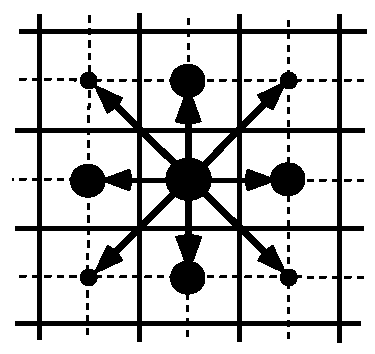
\includegraphics[width=0.70\textwidth]{./TexFiles/Figures/Fig_LDF_ZDF1.pdf}
\caption {    \label{Fig_LDF_ZDF1}
averaging procedure for isopycnal slope computation.}
\end{center}    \end{figure}
%>>>>>>>>>>>>>>>>>>>>>>>>>>>>

%There are three additional questions about the slope calculation. 
%First the expression for the rotation tensor has been obtain assuming the "small slope" approximation, so a bound has to be imposed on slopes. 
%Second, numerical stability issues also require a bound on slopes. 
%Third, the question of boundary condition specified on slopes...

%from griffies: chapter 13.1....



% In addition and also for numerical stability reasons \citep{Cox1987, Griffies_Bk04}, 
% the slopes are bounded by $1/100$ everywhere. This limit is decreasing linearly 
% to zero fom $70$ meters depth and the surface (the fact that the eddies "feel" the 
% surface motivates this flattening of isopycnals near the surface).

For numerical stability reasons \citep{Cox1987, Griffies_Bk04}, the slopes must also 
be bounded by $1/100$ everywhere. This constraint is applied in a piecewise linear 
fashion, increasing from zero at the surface to $1/100$ at $70$ metres and thereafter 
decreasing to zero at the bottom of the ocean. (the fact that the eddies "feel" the 
surface motivates this flattening of isopycnals near the surface).

%>>>>>>>>>>>>>>>>>>>>>>>>>>>>
\begin{figure}[!ht]     \begin{center}
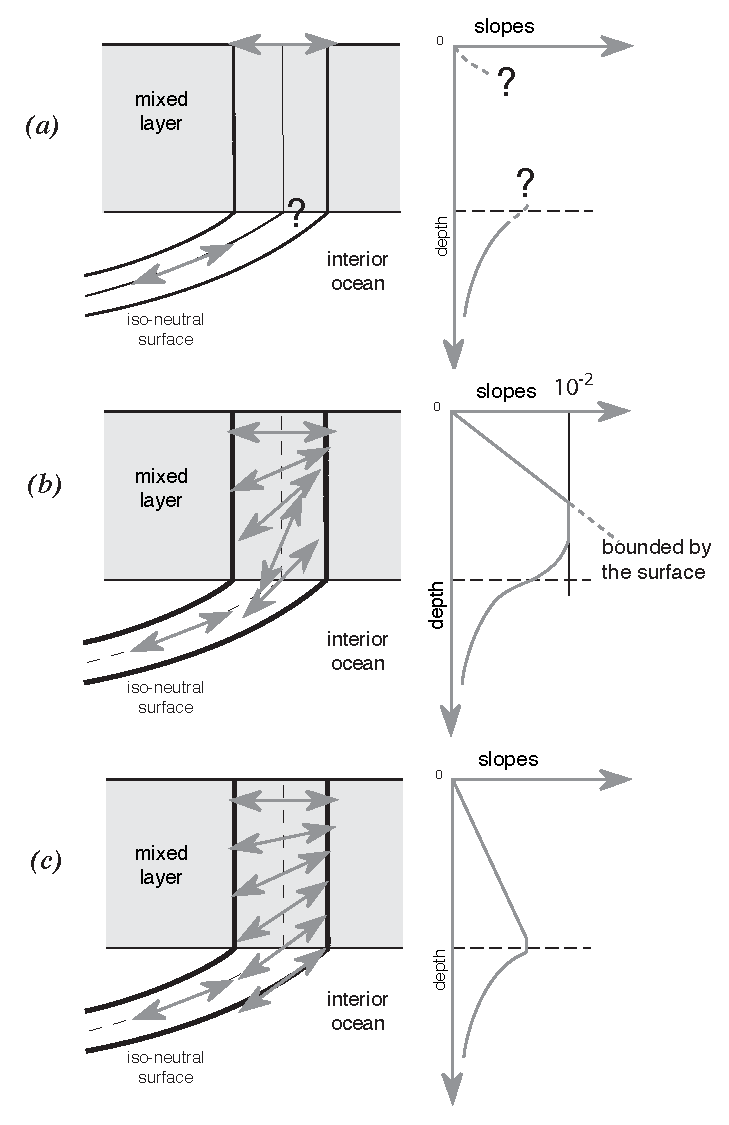
\includegraphics[width=0.70\textwidth]{./TexFiles/Figures/Fig_eiv_slp.pdf}
\caption {     \label{Fig_eiv_slp}
Vertical profile of the slope used for lateral mixing in the mixed layer : 
\textit{(a)} in the real ocean the slope is the iso-neutral slope in the ocean interior, 
which has to be adjusted at the surface boundary (i.e. it must tend to zero at the 
surface since there is no mixing across the air-sea interface: wall boundary 
condition). Nevertheless, the profile between the surface zero value and the interior 
iso-neutral one is unknown, and especially the value at the base of the mixed layer ; 
\textit{(b)} profile of slope using a linear tapering of the slope near the surface and 
imposing a maximum slope of 1/100 ; \textit{(c)} profile of slope actually used in 
\NEMO: a linear decrease of the slope from zero at the surface to its ocean interior 
value computed just below the mixed layer. Note the huge change in the slope at the 
base of the mixed layer between  \textit{(b)}  and \textit{(c)}.}
\end{center}   \end{figure}
%>>>>>>>>>>>>>>>>>>>>>>>>>>>>

\colorbox{yellow}{add here a discussion about the flattening of the slopes, vs  tapering the coefficient.}

\subsection{slopes for momentum iso-neutral mixing}

The iso-neutral diffusion operator on momentum is the same as the one used on 
tracers but applied to each component of the velocity separately (see 
\eqref{Eq_dyn_ldf_iso} in section~\ref{DYN_ldf_iso}). The slopes between the 
surface along which the diffusion operator acts and the surface of computation 
($z$- or $s$-surfaces) are defined at $T$-, $f$-, and \textit{uw}- points for the 
$u$-component, and $T$-, $f$- and \textit{vw}- points for the $v$-component. 
They are computed from the slopes used for tracer diffusion, $i.e.$ 
\eqref{Eq_ldfslp_geo} and \eqref{Eq_ldfslp_iso} :

\begin{equation} \label{Eq_ldfslp_dyn}
\begin{aligned}
&r_{1t}\ \ = \overline{r_{1u}}^{\,i}       &&&    r_{1f}\ \ &= \overline{r_{1u}}^{\,i+1/2} \\
&r_{2f} \ \ = \overline{r_{2v}}^{\,j+1/2} &&& 	r_{2t}\ &= \overline{r_{2v}}^{\,j} \\
&r_{1uw}  = \overline{r_{1w}}^{\,i+1/2} &&\ \ \text{and} \ \ &   r_{1vw}&= \overline{r_{1w}}^{\,j+1/2} \\
&r_{2uw}= \overline{r_{2w}}^{\,j+1/2} &&&         r_{2vw}&= \overline{r_{2w}}^{\,j+1/2}\\
\end{aligned}
\end{equation}

The major issue remaining is in the specification of the boundary conditions. 
The same boundary conditions are chosen as those used for lateral 
diffusion along model level surfaces, i.e. using the shear computed along 
the model levels and with no additional friction at the ocean bottom (see 
{\S\ref{LBC_coast}).


% ================================================================
% Eddy Induced Mixing
% ================================================================
\section  [Eddy Induced Velocity (\textit{traadv\_eiv}, \textit{ldfeiv})]
		{Eddy Induced Velocity (\mdl{traadv\_eiv}, \mdl{ldfeiv})}
\label{LDF_eiv}

When Gent and McWilliams [1990] diffusion is used (\key{traldf\_eiv} defined), 
an eddy induced tracer advection term is added, the formulation of which 
depends on the slopes of iso-neutral surfaces. Contrary to the case of iso-neutral 
mixing, the slopes used here are referenced to the geopotential surfaces, $i.e.$ 
\eqref{Eq_ldfslp_geo} is used in $z$-coordinates, and the sum \eqref{Eq_ldfslp_geo}  
+ \eqref{Eq_ldfslp_iso} in $s$-coordinates. The eddy induced velocity is given by: 
\begin{equation} \label{Eq_ldfeiv}
\begin{split}
 u^* & = \frac{1}{e_{2u}e_{3u}}\; \delta_k \left[e_{2u} \, A_{uw}^{eiv} \; \overline{r_{1w}}^{\,i+1/2} \right]\\
v^* & = \frac{1}{e_{1u}e_{3v}}\; \delta_k \left[e_{1v} \, A_{vw}^{eiv} \; \overline{r_{2w}}^{\,j+1/2} \right]\\
w^* & = \frac{1}{e_{1w}e_{2w}}\; \left\{ \delta_i \left[e_{2u} \, A_{uw}^{eiv} \; \overline{r_{1w}}^{\,i+1/2} \right] + \delta_j \left[e_{1v} \, A_{vw}^{eiv} \; \overline{r_{2w}}^{\,j+1/2} \right] \right\} \\
\end{split}
\end{equation}
where $A^{eiv}$ is the eddy induced velocity coefficient whose value is set 
through \np{rn\_aeiv}, a \textit{nam\_traldf} namelist parameter. 
The three components of the eddy induced velocity are computed and add 
to the eulerian velocity in \mdl{traadv\_eiv}. This has been preferred to a 
separate computation of the advective trends associated with the eiv velocity, 
since it allows us to take advantage of all the advection schemes offered for 
the tracers (see \S\ref{TRA_adv}) and not just the $2^{nd}$ order advection 
scheme as in previous releases of OPA \citep{Madec1998}. This is particularly 
useful for passive tracers where \emph{positivity} of the advection scheme is 
of paramount importance. 

At the surface, lateral and bottom boundaries, the eddy induced velocity, 
and thus the advective eddy fluxes of heat and salt, are set to zero. 





			% Lateral diffusion

% ================================================================
% Chapter  Vertical Ocean Physics (ZDF)
% ================================================================
\chapter{Vertical Ocean Physics (ZDF)}
\label{ZDF}
\minitoc

%gm% Add here a small introduction to ZDF and naming of the different physics (similar to what have been written for TRA and DYN.


\newpage
$\ $\newline    % force a new ligne


% ================================================================
% Vertical Mixing
% ================================================================
\section{Vertical Mixing}
\label{ZDF_zdf}

The discrete form of the ocean subgrid scale physics has been presented in 
\S\ref{TRA_zdf} and \S\ref{DYN_zdf}. At the surface and bottom boundaries, 
the turbulent fluxes of momentum, heat and salt have to be defined. At the 
surface they are prescribed from the surface forcing (see Chap.~\ref{SBC}), 
while at the bottom they are set to zero for heat and salt, unless a geothermal 
flux forcing is prescribed as a bottom boundary condition ($i.e.$ \key{trabbl} 
defined, see \S\ref{TRA_bbc}), and specified through a bottom friction 
parameterisation for momentum (see \S\ref{ZDF_bfr}).

In this section we briefly discuss the various choices offered to compute 
the vertical eddy viscosity and diffusivity coefficients, $A_u^{vm}$ , 
$A_v^{vm}$ and $A^{vT}$ ($A^{vS}$), defined at $uw$-, $vw$- and $w$- 
points, respectively (see \S\ref{TRA_zdf} and \S\ref{DYN_zdf}). These 
coefficients can be assumed to be either constant, or a function of the local 
Richardson number, or computed from a turbulent closure model (either 
TKE or KPP formulation). The computation of these coefficients is initialized 
in the \mdl{zdfini} module and performed in the \mdl{zdfric}, \mdl{zdftke} or 
\mdl{zdfkpp} modules. The trends due to the vertical momentum and tracer 
diffusion, including the surface forcing, are computed and added to the 
general trend in the \mdl{dynzdf} and \mdl{trazdf} modules, respectively. 
These trends can be computed using either a forward time stepping scheme 
(namelist parameter \np{ln\_zdfexp}=true) or a backward time stepping 
scheme (\np{ln\_zdfexp}=false) depending on the magnitude of the mixing 
coefficients, and thus of the formulation used (see \S\ref{STP}).

% -------------------------------------------------------------------------------------------------------------
%        Constant 
% -------------------------------------------------------------------------------------------------------------
\subsection{Constant (\key{zdfcst})}
\label{ZDF_cst}
%--------------------------------------------namzdf---------------------------------------------------------
\namdisplay{namzdf}
%--------------------------------------------------------------------------------------------------------------

Options are defined through the  \ngn{namzdf} namelist variables.
When \key{zdfcst} is defined, the momentum and tracer vertical eddy coefficients 
are set to constant values over the whole ocean. This is the crudest way to define 
the vertical ocean physics. It is recommended that this option is only used in 
process studies, not in basin scale simulations. Typical values used in this case are:
\begin{align*} 
A_u^{vm} = A_v^{vm} &= 1.2\ 10^{-4}~m^2.s^{-1} 	\\
A^{vT} = A^{vS} &= 1.2\ 10^{-5}~m^2.s^{-1}
\end{align*}

These values are set through the \np{rn\_avm0} and \np{rn\_avt0} namelist parameters. 
In all cases, do not use values smaller that those associated with the molecular 
viscosity and diffusivity, that is $\sim10^{-6}~m^2.s^{-1}$ for momentum, 
$\sim10^{-7}~m^2.s^{-1}$ for temperature and $\sim10^{-9}~m^2.s^{-1}$ for salinity.


% -------------------------------------------------------------------------------------------------------------
%        Richardson Number Dependent
% -------------------------------------------------------------------------------------------------------------
\subsection{Richardson Number Dependent (\key{zdfric})}
\label{ZDF_ric}

%--------------------------------------------namric---------------------------------------------------------
\namdisplay{namzdf_ric}
%--------------------------------------------------------------------------------------------------------------

When \key{zdfric} is defined, a local Richardson number dependent formulation 
for the vertical momentum and tracer eddy coefficients is set through the  \ngn{namzdf\_ric} 
namelist variables.The vertical mixing 
coefficients are diagnosed from the large scale variables computed by the model. 
\textit{In situ} measurements have been used to link vertical turbulent activity to 
large scale ocean structures. The hypothesis of a mixing mainly maintained by the 
growth of Kelvin-Helmholtz like instabilities leads to a dependency between the 
vertical eddy coefficients and the local Richardson number ($i.e.$ the 
ratio of stratification to vertical shear). Following \citet{Pacanowski_Philander_JPO81}, the following 
formulation has been implemented:
\begin{equation} \label{Eq_zdfric}
   \left\{      \begin{aligned}
         A^{vT} &= \frac {A_{ric}^{vT}}{\left( 1+a \; Ri \right)^n} + A_b^{vT}       \\
         A^{vm} &= \frac{A^{vT}        }{\left( 1+ a \;Ri  \right)   } + A_b^{vm}
   \end{aligned}    \right.
\end{equation}
where $Ri = N^2 / \left(\partial_z \textbf{U}_h \right)^2$ is the local Richardson 
number, $N$ is the local Brunt-Vais\"{a}l\"{a} frequency (see \S\ref{TRA_bn2}), 
$A_b^{vT} $ and $A_b^{vm}$ are the constant background values set as in the 
constant case (see \S\ref{ZDF_cst}), and $A_{ric}^{vT} = 10^{-4}~m^2.s^{-1}$ 
is the maximum value that can be reached by the coefficient when $Ri\leq 0$, 
$a=5$ and $n=2$. The last three values can be modified by setting the 
\np{rn\_avmri}, \np{rn\_alp} and \np{nn\_ric} namelist parameters, respectively.

A simple mixing-layer model to transfer and dissipate the atmospheric
 forcings (wind-stress and buoyancy fluxes) can be activated setting 
the \np{ln\_mldw} =.true. in the namelist.

In this case, the local depth of turbulent wind-mixing or "Ekman depth"
 $h_{e}(x,y,t)$ is evaluated and the vertical eddy coefficients prescribed within this layer.

This depth is assumed proportional to the "depth of frictional influence" that is limited by rotation:
\begin{equation}
         h_{e} = Ek \frac {u^{*}} {f_{0}}  	\\
\end{equation}
where, $Ek$ is an empirical parameter, $u^{*}$ is the friction velocity and $f_{0}$ is the Coriolis 
parameter.

In this similarity height relationship, the turbulent friction velocity:
\begin{equation}
         u^{*} = \sqrt \frac {|\tau|} {\rho_o}  	\\
\end{equation}

is computed from the wind stress vector $|\tau|$ and the reference density $ \rho_o$.
The final $h_{e}$ is further constrained by the adjustable bounds \np{rn\_mldmin} and \np{rn\_mldmax}.
Once $h_{e}$ is computed, the vertical eddy coefficients within $h_{e}$ are set to 
the empirical values \np{rn\_wtmix} and \np{rn\_wvmix} \citep{Lermusiaux2001}.

% -------------------------------------------------------------------------------------------------------------
%        TKE Turbulent Closure Scheme 
% -------------------------------------------------------------------------------------------------------------
\subsection{TKE Turbulent Closure Scheme (\key{zdftke})}
\label{ZDF_tke}

%--------------------------------------------namzdf_tke--------------------------------------------------
\namdisplay{namzdf_tke}
%--------------------------------------------------------------------------------------------------------------

The vertical eddy viscosity and diffusivity coefficients are computed from a TKE 
turbulent closure model based on a prognostic equation for $\bar{e}$, the turbulent 
kinetic energy, and a closure assumption for the turbulent length scales. This 
turbulent closure model has been developed by \citet{Bougeault1989} in the 
atmospheric case, adapted by \citet{Gaspar1990} for the oceanic case, and 
embedded in OPA, the ancestor of NEMO, by \citet{Blanke1993} for equatorial Atlantic 
simulations. Since then, significant modifications have been introduced by 
\citet{Madec1998} in both the implementation and the formulation of the mixing 
length scale. The time evolution of $\bar{e}$ is the result of the production of 
$\bar{e}$ through vertical shear, its destruction through stratification, its vertical 
diffusion, and its dissipation of \citet{Kolmogorov1942} type:
\begin{equation} \label{Eq_zdftke_e}
\frac{\partial \bar{e}}{\partial t} = 
\frac{K_m}{{e_3}^2 }\;\left[ {\left( {\frac{\partial u}{\partial k}} \right)^2
				        +\left( {\frac{\partial v}{\partial k}} \right)^2} \right]
-K_\rho\,N^2
+\frac{1}{e_3}	\;\frac{\partial }{\partial k}\left[ {\frac{A^{vm}}{e_3 }
				\;\frac{\partial \bar{e}}{\partial k}} \right]
- c_\epsilon \;\frac{\bar {e}^{3/2}}{l_\epsilon }
\end{equation}
\begin{equation} \label{Eq_zdftke_kz}
   \begin{split}
         K_m &= C_k\  l_k\  \sqrt {\bar{e}\; }  	\\
         K_\rho &= A^{vm} / P_{rt}
   \end{split}
\end{equation}
where $N$ is the local Brunt-Vais\"{a}l\"{a} frequency (see \S\ref{TRA_bn2}), 
$l_{\epsilon }$ and $l_{\kappa }$ are the dissipation and mixing length scales, 
$P_{rt}$ is the Prandtl number, $K_m$ and $K_\rho$ are the vertical eddy viscosity 
and diffusivity coefficients. The constants $C_k =  0.1$ and $C_\epsilon = \sqrt {2} /2$  
$\approx 0.7$ are designed to deal with vertical mixing at any depth \citep{Gaspar1990}. 
They are set through namelist parameters \np{nn\_ediff} and \np{nn\_ediss}. 
$P_{rt}$ can be set to unity or, following \citet{Blanke1993}, be a function 
of the local Richardson number, $R_i$:
\begin{align*} \label{Eq_prt}
P_{rt} = \begin{cases}
                    \ \ \ 1 &      \text{if $\ R_i \leq 0.2$} 	\\
                    5\,R_i &      \text{if $\ 0.2 \leq R_i \leq 2$} 	\\
                    \ \ 10 &      \text{if $\ 2 \leq R_i$} 
            \end{cases}
\end{align*}
Options are defined through the  \ngn{namzdfy\_tke} namelist variables.
The choice of $P_{rt}$ is controlled by the \np{nn\_pdl} namelist variable.

At the sea surface, the value of $\bar{e}$ is prescribed from the wind 
stress field as $\bar{e}_o = e_{bb} |\tau| / \rho_o$, with $e_{bb}$ the \np{rn\_ebb} 
namelist parameter. The default value of $e_{bb}$ is 3.75. \citep{Gaspar1990}), 
however a much larger value can be used when taking into account the 
surface wave breaking (see below Eq. \eqref{ZDF_Esbc}). 
The bottom value of TKE is assumed to be equal to the value of the level just above. 
The time integration of the $\bar{e}$ equation may formally lead to negative values 
because the numerical scheme does not ensure its positivity. To overcome this 
problem, a cut-off in the minimum value of $\bar{e}$ is used (\np{rn\_emin} 
namelist parameter). Following \citet{Gaspar1990}, the cut-off value is set 
to $\sqrt{2}/2~10^{-6}~m^2.s^{-2}$. This allows the subsequent formulations 
to match that of \citet{Gargett1984} for the diffusion in the thermocline and 
deep ocean :  $K_\rho = 10^{-3} / N$. 
In addition, a cut-off is applied on $K_m$ and $K_\rho$ to avoid numerical 
instabilities associated with too weak vertical diffusion. They must be 
specified at least larger than the molecular values, and are set through 
\np{rn\_avm0} and \np{rn\_avt0} (namzdf namelist, see \S\ref{ZDF_cst}).

\subsubsection{Turbulent length scale}
For computational efficiency, the original formulation of the turbulent length 
scales proposed by \citet{Gaspar1990} has been simplified. Four formulations 
are proposed, the choice of which is controlled by the \np{nn\_mxl} namelist 
parameter. The first two are based on the following first order approximation 
\citep{Blanke1993}:
\begin{equation} \label{Eq_tke_mxl0_1}
l_k = l_\epsilon = \sqrt {2 \bar{e}\; } / N
\end{equation}
which is valid in a stable stratified region with constant values of the Brunt-
Vais\"{a}l\"{a} frequency. The resulting length scale is bounded by the distance 
to the surface or to the bottom (\np{nn\_mxl} = 0) or by the local vertical scale factor 
(\np{nn\_mxl} = 1). \citet{Blanke1993} notice that this simplification has two major 
drawbacks: it makes no sense for locally unstable stratification and the 
computation no longer uses all the information contained in the vertical density 
profile. To overcome these drawbacks, \citet{Madec1998} introduces the 
\np{nn\_mxl} = 2 or 3 cases, which add an extra assumption concerning the vertical 
gradient of the computed length scale. So, the length scales are first evaluated 
as in \eqref{Eq_tke_mxl0_1} and then bounded such that:
\begin{equation} \label{Eq_tke_mxl_constraint}
\frac{1}{e_3 }\left| {\frac{\partial l}{\partial k}} \right| \leq 1
\qquad \text{with }\  l =  l_k = l_\epsilon
\end{equation}
\eqref{Eq_tke_mxl_constraint} means that the vertical variations of the length 
scale cannot be larger than the variations of depth. It provides a better 
approximation of the \citet{Gaspar1990} formulation while being much less 
time consuming. In particular, it allows the length scale to be limited not only 
by the distance to the surface or to the ocean bottom but also by the distance 
to a strongly stratified portion of the water column such as the thermocline 
(Fig.~\ref{Fig_mixing_length}). In order to impose the \eqref{Eq_tke_mxl_constraint} 
constraint, we introduce two additional length scales: $l_{up}$ and $l_{dwn}$, 
the upward and downward length scales, and evaluate the dissipation and 
mixing length scales as (and note that here we use numerical indexing):
%>>>>>>>>>>>>>>>>>>>>>>>>>>>>
\begin{figure}[!t] \begin{center}
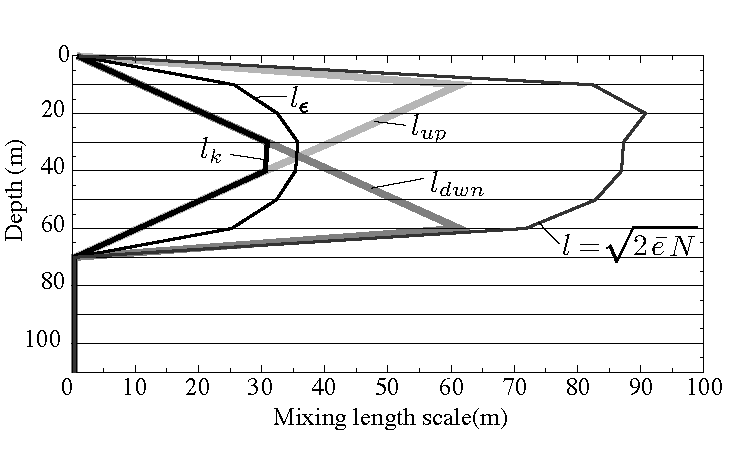
\includegraphics[width=1.00\textwidth]{./TexFiles/Figures/Fig_mixing_length.pdf}
\caption{ \label{Fig_mixing_length} 
Illustration of the mixing length computation. }
\end{center}  
\end{figure}
%>>>>>>>>>>>>>>>>>>>>>>>>>>>>
\begin{equation} \label{Eq_tke_mxl2}
\begin{aligned}
 l_{up\ \ }^{(k)} &= \min \left(  l^{(k)} \ , \ l_{up}^{(k+1)} + e_{3t}^{(k)}\ \ \ \;  \right)
    \quad &\text{ from $k=1$ to $jpk$ }\ \\
 l_{dwn}^{(k)} &= \min \left(  l^{(k)} \ , \ l_{dwn}^{(k-1)} + e_{3t}^{(k-1)}  \right)   
    \quad &\text{ from $k=jpk$ to $1$ }\ \\
\end{aligned}
\end{equation}
where $l^{(k)}$ is computed using \eqref{Eq_tke_mxl0_1}, 
$i.e.$ $l^{(k)} = \sqrt {2 {\bar e}^{(k)} / {N^2}^{(k)} }$.

In the \np{nn\_mxl}~=~2 case, the dissipation and mixing length scales take the same 
value: $ l_k=  l_\epsilon = \min \left(\ l_{up} \;,\;  l_{dwn}\ \right)$, while in the 
\np{nn\_mxl}~=~3 case, the dissipation and mixing turbulent length scales are give 
as in \citet{Gaspar1990}:
\begin{equation} \label{Eq_tke_mxl_gaspar}
\begin{aligned}
& l_k          = \sqrt{\  l_{up} \ \ l_{dwn}\ }  	\\
& l_\epsilon = \min \left(\ l_{up} \;,\;  l_{dwn}\ \right) 
\end{aligned}
\end{equation}

At the ocean surface, a non zero length scale is set through the  \np{rn\_lmin0} namelist 
parameter. Usually the surface scale is given by $l_o = \kappa \,z_o$ 
where $\kappa = 0.4$ is von Karman's constant and $z_o$ the roughness 
parameter of the surface. Assuming $z_o=0.1$~m \citep{Craig_Banner_JPO94} 
leads to a 0.04~m, the default value of \np{rn\_lsurf}. In the ocean interior 
a minimum length scale is set to recover the molecular viscosity when $\bar{e}$ 
reach its minimum value ($1.10^{-6}= C_k\, l_{min} \,\sqrt{\bar{e}_{min}}$ ).


\subsubsection{Surface wave breaking parameterization}
%-----------------------------------------------------------------------%
Following \citet{Mellor_Blumberg_JPO04}, the TKE turbulence closure model has been modified 
to include the effect of surface wave breaking energetics. This results in a reduction of summertime 
surface temperature when the mixed layer is relatively shallow. The \citet{Mellor_Blumberg_JPO04} 
modifications acts on surface length scale and TKE values and air-sea drag coefficient. 
The latter concerns the bulk formulea and is not discussed here. 

Following \citet{Craig_Banner_JPO94}, the boundary condition on surface TKE value is :
\begin{equation}  \label{ZDF_Esbc}
\bar{e}_o = \frac{1}{2}\,\left(  15.8\,\alpha_{CB} \right)^{2/3} \,\frac{|\tau|}{\rho_o}
\end{equation}
where $\alpha_{CB}$ is the \citet{Craig_Banner_JPO94} constant of proportionality 
which depends on the ''wave age'', ranging from 57 for mature waves to 146 for 
younger waves \citep{Mellor_Blumberg_JPO04}. 
The boundary condition on the turbulent length scale follows the Charnock's relation:
\begin{equation} \label{ZDF_Lsbc}
l_o = \kappa \beta \,\frac{|\tau|}{g\,\rho_o}
\end{equation}
where $\kappa=0.40$ is the von Karman constant, and $\beta$ is the Charnock's constant.
\citet{Mellor_Blumberg_JPO04} suggest $\beta = 2.10^{5}$ the value chosen by \citet{Stacey_JPO99}
citing observation evidence, and $\alpha_{CB} = 100$ the Craig and Banner's value.
As the surface boundary condition on TKE is prescribed through $\bar{e}_o = e_{bb} |\tau| / \rho_o$, 
with $e_{bb}$ the \np{rn\_ebb} namelist parameter, setting \np{rn\_ebb}~=~67.83 corresponds 
to $\alpha_{CB} = 100$. further setting  \np{ln\_lsurf} to true applies \eqref{ZDF_Lsbc} 
as surface boundary condition on length scale, with $\beta$ hard coded to the Stacet's value.
Note that a minimal threshold of \np{rn\_emin0}$=10^{-4}~m^2.s^{-2}$ (namelist parameters) 
is applied on surface $\bar{e}$ value.


\subsubsection{Langmuir cells}
%--------------------------------------%
Langmuir circulations (LC) can be described as ordered large-scale vertical motions 
in the surface layer of the oceans. Although LC have nothing to do with convection, 
the circulation pattern is rather similar to so-called convective rolls in the atmospheric 
boundary layer. The detailed physics behind LC is described in, for example, 
\citet{Craik_Leibovich_JFM76}. The prevailing explanation is that LC arise from 
a nonlinear interaction between the Stokes drift and wind drift currents. 

Here we introduced in the TKE turbulent closure the simple parameterization of 
Langmuir circulations proposed by \citep{Axell_JGR02} for a $k-\epsilon$ turbulent closure. 
The parameterization, tuned against large-eddy simulation, includes the whole effect
of LC in an extra source terms of TKE, $P_{LC}$.
The presence of $P_{LC}$ in \eqref{Eq_zdftke_e}, the TKE equation, is controlled 
by setting \np{ln\_lc} to \textit{true} in the namtke namelist.
 
By making an analogy with the characteristic convective velocity scale 
($e.g.$, \citet{D'Alessio_al_JPO98}), $P_{LC}$ is assumed to be : 
\begin{equation}
P_{LC}(z) = \frac{w_{LC}^3(z)}{H_{LC}}
\end{equation}
where $w_{LC}(z)$ is the vertical velocity profile of LC, and $H_{LC}$ is the LC depth.
With no information about the wave field, $w_{LC}$ is assumed to be proportional to 
the Stokes drift $u_s = 0.377\,\,|\tau|^{1/2}$, where $|\tau|$ is the surface wind stress module 
\footnote{Following \citet{Li_Garrett_JMR93}, the surface Stoke drift velocity
may be expressed as $u_s =  0.016 \,|U_{10m}|$. Assuming an air density of 
$\rho_a=1.22 \,Kg/m^3$ and a drag coefficient of $1.5~10^{-3}$ give the expression 
used of $u_s$ as a function of the module of surface stress}. 
For the vertical variation, $w_{LC}$ is assumed to be zero at the surface as well as 
at a finite depth $H_{LC}$ (which is often close to the mixed layer depth), and simply 
varies as a sine function in between (a first-order profile for the Langmuir cell structures). 
The resulting expression for $w_{LC}$ is :
\begin{equation}
w_{LC}  = \begin{cases}
                   c_{LC} \,u_s \,\sin(- \pi\,z / H_{LC} )    &      \text{if $-z \leq H_{LC}$} 	\\
                   0                 				 &      \text{otherwise} 
                 \end{cases}
\end{equation}
where $c_{LC} = 0.15$ has been chosen by \citep{Axell_JGR02} as a good compromise 
to fit LES data. The chosen value yields maximum vertical velocities $w_{LC}$ of the order 
of a few centimeters per second. The value of $c_{LC}$ is set through the \np{rn\_lc} 
namelist parameter, having in mind that it should stay between 0.15 and 0.54 \citep{Axell_JGR02}. 

The $H_{LC}$ is estimated in a similar way as the turbulent length scale of TKE equations:
$H_{LC}$ is depth to which a water parcel with kinetic energy due to Stoke drift
can reach on its own by converting its kinetic energy to potential energy, according to 
\begin{equation}
- \int_{-H_{LC}}^0 { N^2\;z  \;dz} = \frac{1}{2} u_s^2
\end{equation}


\subsubsection{Mixing just below the mixed layer}
%--------------------------------------------------------------%

To be add here a description of "penetration of TKE" and the associated namelist parameters
 \np{nn\_etau}, \np{rn\_efr} and \np{nn\_htau}.

% from Burchard et al OM 2008 : 
% the most critical process not reproduced by statistical turbulence models is the activity of internal waves and their interaction with turbulence. After the Reynolds decomposition, internal waves are in principle included in the RANS equations, but later partially excluded by the hydrostatic assumption and the model resolution. Thus far, the representation of internal wave mixing in ocean models has been relatively crude (e.g. Mellor, 1989; Large et al., 1994; Meier, 2001; Axell, 2002; St. Laurent and Garrett, 2002).



% -------------------------------------------------------------------------------------------------------------
%        TKE discretization considerations
% -------------------------------------------------------------------------------------------------------------
\subsection{TKE discretization considerations (\key{zdftke})}
\label{ZDF_tke_ene}

%>>>>>>>>>>>>>>>>>>>>>>>>>>>>
\begin{figure}[!t]   \begin{center}
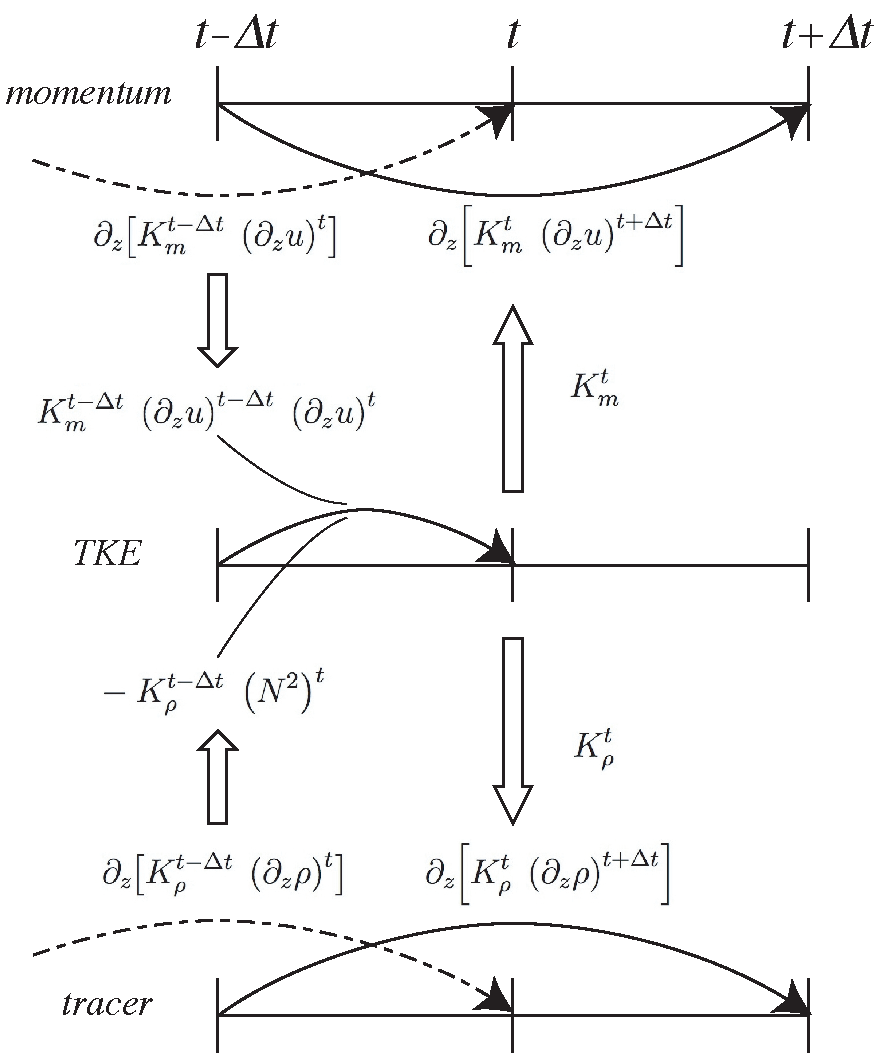
\includegraphics[width=1.00\textwidth]{./TexFiles/Figures/Fig_ZDF_TKE_time_scheme.pdf}
\caption{ \label{Fig_TKE_time_scheme} 
Illustration of the TKE time integration and its links to the momentum and tracer time integration. }
\end{center}  
\end{figure}
%>>>>>>>>>>>>>>>>>>>>>>>>>>>>

The production of turbulence by vertical shear (the first term of the right hand side 
of \eqref{Eq_zdftke_e}) should balance the loss of kinetic energy associated with
the vertical momentum diffusion (first line in \eqref{Eq_PE_zdf}). To do so a special care 
have to be taken for both the time and space discretization of the TKE equation 
\citep{Burchard_OM02,Marsaleix_al_OM08}.

Let us first address the time stepping issue. Fig.~\ref{Fig_TKE_time_scheme} shows 
how the two-level Leap-Frog time stepping of the momentum and tracer equations interplays 
with the one-level forward time stepping of TKE equation. With this framework, the total loss 
of kinetic energy (in 1D for the demonstration) due to the vertical momentum diffusion is 
obtained by multiplying this quantity by $u^t$ and summing the result vertically:   
\begin{equation} \label{Eq_energ1}
\begin{split}
\int_{-H}^{\eta}  u^t \,\partial_z &\left( {K_m}^t \,(\partial_z u)^{t+\rdt}  \right) \,dz   \\
&= \Bigl[  u^t \,{K_m}^t \,(\partial_z u)^{t+\rdt} \Bigr]_{-H}^{\eta}          
 - \int_{-H}^{\eta}{ {K_m}^t \,\partial_z{u^t} \,\partial_z u^{t+\rdt} \,dz }
\end{split}
\end{equation}
Here, the vertical diffusion of momentum is discretized backward in time 
with a coefficient, $K_m$, known at time $t$ (Fig.~\ref{Fig_TKE_time_scheme}), 
as it is required when using the TKE scheme (see \S\ref{STP_forward_imp}). 
The first term of the right hand side of \eqref{Eq_energ1} represents the kinetic energy 
transfer at the surface (atmospheric forcing) and at the bottom (friction effect). 
The second term is always negative. It is the dissipation rate of kinetic energy, 
and thus minus the shear production rate of $\bar{e}$. \eqref{Eq_energ1} 
implies that, to be energetically consistent, the production rate of $\bar{e}$ 
used to compute $(\bar{e})^t$ (and thus ${K_m}^t$) should be expressed as 
${K_m}^{t-\rdt}\,(\partial_z u)^{t-\rdt} \,(\partial_z u)^t$ (and not by the more straightforward 
$K_m \left( \partial_z u \right)^2$ expression taken at time $t$ or $t-\rdt$).

A similar consideration applies on the destruction rate of $\bar{e}$ due to stratification 
(second term of the right hand side of \eqref{Eq_zdftke_e}). This term 
must balance the input of potential energy resulting from vertical mixing. 
The rate of change of potential energy (in 1D for the demonstration) due vertical 
mixing is obtained by multiplying vertical density diffusion 
tendency by $g\,z$ and and summing the result vertically:
\begin{equation} \label{Eq_energ2}
\begin{split}
\int_{-H}^{\eta} g\,z\,\partial_z &\left( {K_\rho}^t \,(\partial_k \rho)^{t+\rdt}   \right) \,dz    \\
&= \Bigl[  g\,z \,{K_\rho}^t \,(\partial_z \rho)^{t+\rdt} \Bigr]_{-H}^{\eta}  
   - \int_{-H}^{\eta}{ g \,{K_\rho}^t \,(\partial_k \rho)^{t+\rdt} } \,dz   \\
&= - \Bigl[  z\,{K_\rho}^t \,(N^2)^{t+\rdt} \Bigr]_{-H}^{\eta}
+ \int_{-H}^{\eta}{  \rho^{t+\rdt} \, {K_\rho}^t \,(N^2)^{t+\rdt} \,dz  }
\end{split}
\end{equation}
where we use $N^2 = -g \,\partial_k \rho / (e_3 \rho)$. 
The first term of the right hand side of \eqref{Eq_energ2}  is always zero 
because there is no diffusive flux through the ocean surface and bottom). 
The second term is minus the destruction rate of  $\bar{e}$ due to stratification. 
Therefore \eqref{Eq_energ1} implies that, to be energetically consistent, the product 
${K_\rho}^{t-\rdt}\,(N^2)^t$ should be used in \eqref{Eq_zdftke_e}, the TKE equation.

Let us now address the space discretization issue. 
The vertical eddy coefficients are defined at $w$-point whereas the horizontal velocity 
components are in the centre of the side faces of a $t$-box in staggered C-grid 
(Fig.\ref{Fig_cell}). A space averaging is thus required to obtain the shear TKE production term.
By redoing the \eqref{Eq_energ1} in the 3D case, it can be shown that the product of 
eddy coefficient by the shear at $t$ and $t-\rdt$ must be performed prior to the averaging.
Furthermore, the possible time variation of $e_3$ (\key{vvl} case) have to be taken into 
account.

The above energetic considerations leads to 
the following final discrete form for the TKE equation:
\begin{equation} \label{Eq_zdftke_ene}
\begin{split}
\frac { (\bar{e})^t - (\bar{e})^{t-\rdt} } {\rdt}  \equiv  
\Biggl\{ \Biggr.
  &\overline{ \left( \left(\overline{K_m}^{\,i+1/2}\right)^{t-\rdt} \,\frac{\delta_{k+1/2}[u^{t+\rdt}]}{{e_3u}^{t+\rdt} } 
                                                                              \ \frac{\delta_{k+1/2}[u^ t         ]}{{e_3u}^ t          }  \right) }^{\,i} \\
+&\overline{  \left( \left(\overline{K_m}^{\,j+1/2}\right)^{t-\rdt} \,\frac{\delta_{k+1/2}[v^{t+\rdt}]}{{e_3v}^{t+\rdt} } 
                                                                               \ \frac{\delta_{k+1/2}[v^ t         ]}{{e_3v}^ t          }  \right) }^{\,j} 
\Biggr. \Biggr\}   \\
%
- &{K_\rho}^{t-\rdt}\,{(N^2)^t}    \\
%
+&\frac{1}{{e_3w}^{t+\rdt}}  \;\delta_{k+1/2} \left[   {K_m}^{t-\rdt} \,\frac{\delta_{k}[(\bar{e})^{t+\rdt}]} {{e_3w}^{t+\rdt}}   \right]   \\
%
- &c_\epsilon \; \left( \frac{\sqrt{\bar {e}}}{l_\epsilon}\right)^{t-\rdt}\,(\bar {e})^{t+\rdt}
\end{split}
\end{equation}
where the last two terms in \eqref{Eq_zdftke_ene} (vertical diffusion and Kolmogorov dissipation) 
are time stepped using a backward scheme (see\S\ref{STP_forward_imp}). 
Note that the Kolmogorov term has been linearized in time in order to render 
the implicit computation possible. The restart of the TKE scheme 
requires the storage of $\bar {e}$, $K_m$, $K_\rho$ and $l_\epsilon$ as they all appear in 
the right hand side of \eqref{Eq_zdftke_ene}. For the latter, it is in fact 
the ratio $\sqrt{\bar{e}}/l_\epsilon$ which is stored. 

% -------------------------------------------------------------------------------------------------------------
%        GLS Generic Length Scale Scheme 
% -------------------------------------------------------------------------------------------------------------
\subsection{GLS Generic Length Scale (\key{zdfgls})}
\label{ZDF_gls}

%--------------------------------------------namzdf_gls---------------------------------------------------------
\namdisplay{namzdf_gls}
%--------------------------------------------------------------------------------------------------------------

The Generic Length Scale (GLS) scheme is a turbulent closure scheme based on 
two prognostic equations: one for the turbulent kinetic energy $\bar {e}$, and another 
for the generic length scale, $\psi$ \citep{Umlauf_Burchard_JMS03, Umlauf_Burchard_CSR05}. 
This later variable is defined as : $\psi = {C_{0\mu}}^{p} \ {\bar{e}}^{m} \ l^{n}$, 
where the triplet $(p, m, n)$ value given in Tab.\ref{Tab_GLS} allows to recover 
a number of well-known turbulent closures ($k$-$kl$ \citep{Mellor_Yamada_1982}, 
$k$-$\epsilon$ \citep{Rodi_1987}, $k$-$\omega$ \citep{Wilcox_1988} 
among others \citep{Umlauf_Burchard_JMS03,Kantha_Carniel_CSR05}). 
The GLS scheme is given by the following set of equations:
\begin{equation} \label{Eq_zdfgls_e}
\frac{\partial \bar{e}}{\partial t} = 
\frac{K_m}{\sigma_e e_3 }\;\left[ {\left( \frac{\partial u}{\partial k} \right)^2
                                                   +\left( \frac{\partial v}{\partial k} \right)^2} \right]
-K_\rho \,N^2
+\frac{1}{e_3}\,\frac{\partial}{\partial k} \left[ \frac{K_m}{e_3}\,\frac{\partial \bar{e}}{\partial k} \right]
- \epsilon
\end{equation}

\begin{equation} \label{Eq_zdfgls_psi}
   \begin{split}
\frac{\partial \psi}{\partial t} =& \frac{\psi}{\bar{e}} \left\{
\frac{C_1\,K_m}{\sigma_{\psi} {e_3}}\;\left[ {\left( \frac{\partial u}{\partial k} \right)^2
                                                                   +\left( \frac{\partial v}{\partial k} \right)^2} \right]
- C_3 \,K_\rho\,N^2   - C_2 \,\epsilon \,Fw   \right\}             \\
&+\frac{1}{e_3}  \;\frac{\partial }{\partial k}\left[ {\frac{K_m}{e_3 }
                                  \;\frac{\partial \psi}{\partial k}} \right]\;
   \end{split}
\end{equation}

\begin{equation} \label{Eq_zdfgls_kz}
   \begin{split}
         K_m    &= C_{\mu} \ \sqrt {\bar{e}} \ l         \\
         K_\rho &= C_{\mu'}\ \sqrt {\bar{e}} \ l
   \end{split}
\end{equation}

\begin{equation} \label{Eq_zdfgls_eps}
{\epsilon} = C_{0\mu} \,\frac{\bar {e}^{3/2}}{l} \;
\end{equation}
where $N$ is the local Brunt-Vais\"{a}l\"{a} frequency (see \S\ref{TRA_bn2}) 
and $\epsilon$ the dissipation rate. 
The constants $C_1$, $C_2$, $C_3$, ${\sigma_e}$, ${\sigma_{\psi}}$ and the wall function ($Fw$) 
depends of the choice of the turbulence model. Four different turbulent models are pre-defined 
(Tab.\ref{Tab_GLS}). They are made available through the \np{nn\_clo} namelist parameter. 

%--------------------------------------------------TABLE--------------------------------------------------
\begin{table}[htbp]	\begin{center}
%\begin{tabular}{cp{70pt}cp{70pt}cp{70pt}cp{70pt}cp{70pt}cp{70pt}c}
\begin{tabular}{ccccc}
          	             &   $k-kl$   & $k-\epsilon$ & $k-\omega$ &   generic   \\  
%                        & \citep{Mellor_Yamada_1982} &  \citep{Rodi_1987}       & \citep{Wilcox_1988} &                 \\  
\hline  \hline 
\np{nn\_clo}     & \textbf{0} &   \textbf{1}  &   \textbf{2}   &    \textbf{3}   \\  
\hline 
$( p , n , m )$	       &   ( 0 , 1 , 1 )   & ( 3 , 1.5 , -1 )   & ( -1 , 0.5 , -1 )    &  ( 2 , 1 , -0.67 )  \\
$\sigma_k$      &    2.44         &     1.              &      2.                &      0.8          \\
$\sigma_\psi$  &    2.44         &     1.3            &      2.                 &       1.07       \\
$C_1$              &      0.9         &     1.44          &      0.555          &       1.           \\
$C_2$              &      0.5         &     1.92          &      0.833          &       1.22       \\
$C_3$              &      1.           &     1.              &      1.                &       1.           \\
$F_{wall}$        &      Yes        &       --             &     --                  &      --          \\
\hline
\hline
\end{tabular}
\caption{   \label{Tab_GLS} 
Set of predefined GLS parameters, or equivalently predefined turbulence models available 
with \key{zdfgls} and controlled by the \np{nn\_clos} namelist variable in \ngn{namzdf\_gls} .}
\end{center}	\end{table}
%--------------------------------------------------------------------------------------------------------------

In the Mellor-Yamada model, the negativity of $n$ allows to use a wall function to force
the convergence of the mixing length towards $K z_b$ ($K$: Kappa and $z_b$: rugosity length) 
value near physical boundaries (logarithmic boundary layer law). $C_{\mu}$ and $C_{\mu'}$ 
are calculated from stability function proposed by \citet{Galperin_al_JAS88}, or by \citet{Kantha_Clayson_1994} 
or one of the two functions suggested by \citet{Canuto_2001}  (\np{nn\_stab\_func} = 0, 1, 2 or 3, resp.}). 
The value of $C_{0\mu}$ depends of the choice of the stability function.

The surface and bottom boundary condition on both $\bar{e}$ and $\psi$ can be calculated 
thanks to Dirichlet or Neumann condition through \np{nn\_tkebc\_surf} and \np{nn\_tkebc\_bot}, resp. 
As for TKE closure , the wave effect on the mixing is considered when \np{ln\_crban}~=~true
\citep{Craig_Banner_JPO94, Mellor_Blumberg_JPO04}. The \np{rn\_crban} namelist parameter 
is $\alpha_{CB}$ in \eqref{ZDF_Esbc} and \np{rn\_charn} provides the value of $\beta$ in \eqref{ZDF_Lsbc}. 

The $\psi$ equation is known to fail in stably stratified flows, and for this reason 
almost all authors apply a clipping of the length scale as an \textit{ad hoc} remedy. 
With this clipping, the maximum permissible length scale is determined by 
$l_{max} = c_{lim} \sqrt{2\bar{e}}/ N$. A value of $c_{lim} = 0.53$ is often used 
\citep{Galperin_al_JAS88}. \cite{Umlauf_Burchard_CSR05} show that the value of 
the clipping factor is of crucial importance for the entrainment depth predicted in 
stably stratified situations, and that its value has to be chosen in accordance 
with the algebraic model for the turbulent fluxes. The clipping is only activated 
if \np{ln\_length\_lim}=true, and the $c_{lim}$ is set to the \np{rn\_clim\_galp} value.

The time and space discretization of the GLS equations follows the same energetic 
consideration as for the TKE case described in \S\ref{ZDF_tke_ene}  \citep{Burchard_OM02}. 
Examples of performance of the 4 turbulent closure scheme can be found in \citet{Warner_al_OM05}.

% -------------------------------------------------------------------------------------------------------------
%        K Profile Parametrisation (KPP) 
% -------------------------------------------------------------------------------------------------------------
\subsection{K Profile Parametrisation (KPP) (\key{zdfkpp}) }
\label{ZDF_kpp}

%--------------------------------------------namkpp--------------------------------------------------------
\namdisplay{namzdf_kpp}
%--------------------------------------------------------------------------------------------------------------

The KKP scheme has been implemented by J. Chanut ...
Options are defined through the  \ngn{namzdf\_kpp} namelist variables.

\colorbox{yellow}{Add a description of KPP here.}


% ================================================================
% Convection
% ================================================================
\section{Convection}
\label{ZDF_conv}

%--------------------------------------------namzdf--------------------------------------------------------
\namdisplay{namzdf}
%--------------------------------------------------------------------------------------------------------------

Static instabilities (i.e. light potential densities under heavy ones) may 
occur at particular ocean grid points. In nature, convective processes 
quickly re-establish the static stability of the water column. These 
processes have been removed from the model via the hydrostatic 
assumption so they must be parameterized. Three parameterisations 
are available to deal with convective processes: a non-penetrative 
convective adjustment or an enhanced vertical diffusion, or/and the 
use of a turbulent closure scheme.

% -------------------------------------------------------------------------------------------------------------
%       Non-Penetrative Convective Adjustment 
% -------------------------------------------------------------------------------------------------------------
\subsection   [Non-Penetrative Convective Adjustment (\np{ln\_tranpc}) ]
			{Non-Penetrative Convective Adjustment (\np{ln\_tranpc}=.true.) }
\label{ZDF_npc}

%--------------------------------------------namzdf--------------------------------------------------------
\namdisplay{namzdf}
%--------------------------------------------------------------------------------------------------------------

%>>>>>>>>>>>>>>>>>>>>>>>>>>>>
\begin{figure}[!htb]  	\begin{center}
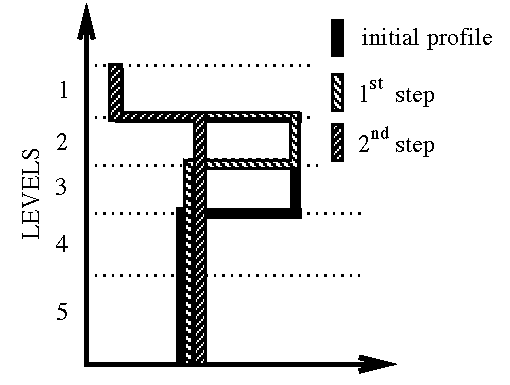
\includegraphics[width=0.90\textwidth]{./TexFiles/Figures/Fig_npc.pdf}
\caption{  \label{Fig_npc} 
Example of an unstable density profile treated by the non penetrative 
convective adjustment algorithm. $1^{st}$ step: the initial profile is checked from 
the surface to the bottom. It is found to be unstable between levels 3 and 4. 
They are mixed. The resulting $\rho$ is still larger than $\rho$(5): levels 3 to 5 
are mixed. The resulting $\rho$ is still larger than $\rho$(6): levels 3 to 6 are 
mixed. The $1^{st}$ step ends since the density profile is then stable below 
the level 3. $2^{nd}$ step: the new $\rho$ profile is checked following the same 
procedure as in $1^{st}$ step: levels 2 to 5 are mixed. The new density profile 
is checked. It is found stable: end of algorithm.}
\end{center}  	\end{figure}
%>>>>>>>>>>>>>>>>>>>>>>>>>>>>

Options are defined through the  \ngn{namzdf} namelist variables.
The non-penetrative convective adjustment is used when \np{ln\_zdfnpc}=true. 
It is applied at each \np{nn\_npc} time step and mixes downwards instantaneously 
the statically unstable portion of the water column, but only until the density 
structure becomes neutrally stable ($i.e.$ until the mixed portion of the water 
column has \textit{exactly} the density of the water just below) \citep{Madec_al_JPO91}. 
The associated algorithm is an iterative process used in the following way 
(Fig. \ref{Fig_npc}): starting from the top of the ocean, the first instability is 
found. Assume in the following that the instability is located between levels 
$k$ and $k+1$. The potential temperature and salinity in the two levels are 
vertically mixed, conserving the heat and salt contents of the water column. 
The new density is then computed by a linear approximation. If the new 
density profile is still unstable between levels $k+1$ and $k+2$, levels $k$, 
$k+1$ and $k+2$ are then mixed. This process is repeated until stability is 
established below the level $k$ (the mixing process can go down to the 
ocean bottom). The algorithm is repeated to check if the density profile 
between level $k-1$ and $k$ is unstable and/or if there is no deeper instability.

This algorithm is significantly different from mixing statically unstable levels 
two by two. The latter procedure cannot converge with a finite number 
of iterations for some vertical profiles while the algorithm used in \NEMO 
converges for any profile in a number of iterations which is less than the 
number of vertical levels. This property is of paramount importance as 
pointed out by \citet{Killworth1989}: it avoids the existence of permanent 
and unrealistic static instabilities at the sea surface. This non-penetrative 
convective algorithm has been proved successful in studies of the deep 
water formation in the north-western Mediterranean Sea 
\citep{Madec_al_JPO91, Madec_al_DAO91, Madec_Crepon_Bk91}.

Note that in the current implementation of this algorithm presents several 
limitations. First, potential density referenced to the sea surface is used to 
check whether the density profile is stable or not. This is a strong 
simplification which leads to large errors for realistic ocean simulations. 
Indeed, many water masses of the world ocean, especially Antarctic Bottom
Water, are unstable when represented in surface-referenced potential density. 
The scheme will erroneously mix them up. Second, the mixing of potential 
density is assumed to be linear. This assures the convergence of the algorithm 
even when the equation of state is non-linear. Small static instabilities can thus 
persist due to cabbeling: they will be treated at the next time step. 
Third, temperature and salinity, and thus density, are mixed, but the 
corresponding velocity fields remain unchanged. When using a Richardson 
Number dependent eddy viscosity, the mixing of momentum is done through 
the vertical diffusion: after a static adjustment, the Richardson Number is zero 
and thus the eddy viscosity coefficient is at a maximum. When this convective 
adjustment algorithm is used with constant vertical eddy viscosity, spurious 
solutions can occur since the vertical momentum diffusion remains small even 
after a static adjustment. In that case, we recommend the addition of momentum 
mixing in a manner that mimics the mixing in temperature and salinity 
\citep{Speich_PhD92, Speich_al_JPO96}.

% -------------------------------------------------------------------------------------------------------------
%       Enhanced Vertical Diffusion 
% -------------------------------------------------------------------------------------------------------------
\subsection   [Enhanced Vertical Diffusion (\np{ln\_zdfevd})]
			{Enhanced Vertical Diffusion (\np{ln\_zdfevd}=true)}
\label{ZDF_evd}

%--------------------------------------------namzdf--------------------------------------------------------
\namdisplay{namzdf}
%--------------------------------------------------------------------------------------------------------------

Options are defined through the  \ngn{namzdf} namelist variables.
The enhanced vertical diffusion parameterisation is used when \np{ln\_zdfevd}=true. 
In this case, the vertical eddy mixing coefficients are assigned very large values 
(a typical value is $10\;m^2s^{-1})$ in regions where the stratification is unstable 
($i.e.$ when $N^2$ the Brunt-Vais\"{a}l\"{a} frequency is negative) 
\citep{Lazar_PhD97, Lazar_al_JPO99}. This is done either on tracers only 
(\np{nn\_evdm}=0) or on both momentum and tracers (\np{nn\_evdm}=1).

In practice, where $N^2\leq 10^{-12}$, $A_T^{vT}$ and $A_T^{vS}$, and 
if \np{nn\_evdm}=1, the four neighbouring $A_u^{vm} \;\mbox{and}\;A_v^{vm}$ 
values also, are set equal to the namelist parameter \np{rn\_avevd}. A typical value 
for $rn\_avevd$ is between 1 and $100~m^2.s^{-1}$. This parameterisation of 
convective processes is less time consuming than the convective adjustment 
algorithm presented above when mixing both tracers and momentum in the 
case of static instabilities. It requires the use of an implicit time stepping on 
vertical diffusion terms (i.e. \np{ln\_zdfexp}=false). 

Note that the stability test is performed on both \textit{before} and \textit{now} 
values of $N^2$. This removes a potential source of divergence of odd and
even time step in a leapfrog environment \citep{Leclair_PhD2010} (see \S\ref{STP_mLF}).

% -------------------------------------------------------------------------------------------------------------
%       Turbulent Closure Scheme 
% -------------------------------------------------------------------------------------------------------------
\subsection{Turbulent Closure Scheme (\key{zdftke} or \key{zdfgls})}
\label{ZDF_tcs}

The turbulent closure scheme presented in \S\ref{ZDF_tke} and \S\ref{ZDF_gls} 
(\key{zdftke} or \key{zdftke} is defined) in theory solves the problem of statically 
unstable density profiles. In such a case, the term corresponding to the 
destruction of turbulent kinetic energy through stratification in \eqref{Eq_zdftke_e} 
or \eqref{Eq_zdfgls_e} becomes a source term, since $N^2$ is negative. 
It results in large values of $A_T^{vT}$ and  $A_T^{vT}$, and also the four neighbouring 
$A_u^{vm} {and}\;A_v^{vm}$ (up to $1\;m^2s^{-1})$. These large values 
restore the static stability of the water column in a way similar to that of the 
enhanced vertical diffusion parameterisation (\S\ref{ZDF_evd}). However, 
in the vicinity of the sea surface (first ocean layer), the eddy coefficients 
computed by the turbulent closure scheme do not usually exceed $10^{-2}m.s^{-1}$, 
because the mixing length scale is bounded by the distance to the sea surface. 
It can thus be useful to combine the enhanced vertical 
diffusion with the turbulent closure scheme, $i.e.$ setting the \np{ln\_zdfnpc} 
namelist parameter to true and defining the turbulent closure CPP key all together.

The KPP turbulent closure scheme already includes enhanced vertical diffusion 
in the case of convection, as governed by the variables $bvsqcon$ and $difcon$ 
found in \mdl{zdfkpp}, therefore \np{ln\_zdfevd}=false should be used with the KPP 
scheme. %gm%  + one word on non local flux with KPP scheme trakpp.F90 module...

% ================================================================
% Double Diffusion Mixing
% ================================================================
\section  [Double Diffusion Mixing (\key{zdfddm})]
		{Double Diffusion Mixing (\key{zdfddm})}
\label{ZDF_ddm}

%-------------------------------------------namzdf_ddm-------------------------------------------------
\namdisplay{namzdf_ddm}
%--------------------------------------------------------------------------------------------------------------

Options are defined through the  \ngn{namzdf\_ddm} namelist variables.
Double diffusion occurs when relatively warm, salty water overlies cooler, fresher 
water, or vice versa. The former condition leads to salt fingering and the latter 
to diffusive convection. Double-diffusive phenomena contribute to diapycnal 
mixing in extensive regions of the ocean.  \citet{Merryfield1999} include a 
parameterisation of such phenomena in a global ocean model and show that 
it leads to relatively minor changes in circulation but exerts significant regional 
influences on temperature and salinity. This parameterisation has been 
introduced in \mdl{zdfddm} module and is controlled by the \key{zdfddm} CPP key.

Diapycnal mixing of S and T are described by diapycnal diffusion coefficients 
\begin{align*} % \label{Eq_zdfddm_Kz}
    &A^{vT} = A_o^{vT}+A_f^{vT}+A_d^{vT}	\\
    &A^{vS} = A_o^{vS}+A_f^{vS}+A_d^{vS}
\end{align*}
where subscript $f$ represents mixing by salt fingering, $d$ by diffusive convection, 
and $o$ by processes other than double diffusion. The rates of double-diffusive 
mixing depend on the buoyancy ratio $R_\rho = \alpha \partial_z T / \beta \partial_z S$, 
where $\alpha$ and $\beta$ are coefficients of thermal expansion and saline 
contraction (see \S\ref{TRA_eos}). To represent mixing of $S$ and $T$ by salt 
fingering, we adopt the diapycnal diffusivities suggested by Schmitt (1981):
\begin{align} \label{Eq_zdfddm_f}
A_f^{vS} &= 	\begin{cases}
	\frac{A^{\ast v}}{1+(R_\rho / R_c)^n   } &\text{if  $R_\rho > 1$ and $N^2>0$ } \\
	0 				  					    &\text{otherwise} 
				\end{cases}   
\\ 		    \label{Eq_zdfddm_f_T}
A_f^{vT} &= 0.7 \ A_f^{vS} / R_\rho 
\end{align}

%>>>>>>>>>>>>>>>>>>>>>>>>>>>>
\begin{figure}[!t]   \begin{center}
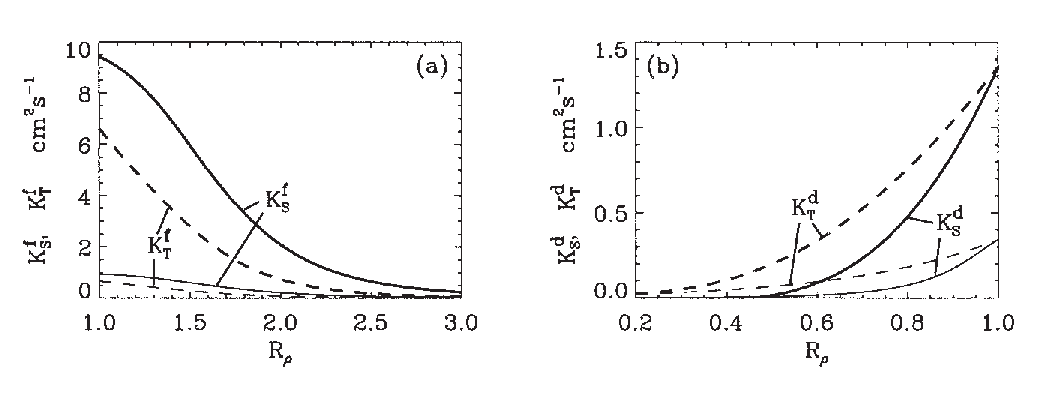
\includegraphics[width=0.99\textwidth]{./TexFiles/Figures/Fig_zdfddm.pdf}
\caption{  \label{Fig_zdfddm}
From \citet{Merryfield1999} : (a) Diapycnal diffusivities $A_f^{vT}$ 
and $A_f^{vS}$ for temperature and salt in regions of salt fingering. Heavy 
curves denote $A^{\ast v} = 10^{-3}~m^2.s^{-1}$ and thin curves 
$A^{\ast v} = 10^{-4}~m^2.s^{-1}$ ; (b) diapycnal diffusivities $A_d^{vT}$ and 
$A_d^{vS}$ for temperature and salt in regions of diffusive convection. Heavy 
curves denote the Federov parameterisation and thin curves the Kelley 
parameterisation. The latter is not implemented in \NEMO. }
\end{center}    \end{figure}
%>>>>>>>>>>>>>>>>>>>>>>>>>>>>

The factor 0.7 in \eqref{Eq_zdfddm_f_T} reflects the measured ratio 
$\alpha F_T /\beta F_S \approx  0.7$ of buoyancy flux of heat to buoyancy 
flux of salt ($e.g.$, \citet{McDougall_Taylor_JMR84}). Following  \citet{Merryfield1999}, 
we adopt $R_c = 1.6$, $n = 6$, and $A^{\ast v} = 10^{-4}~m^2.s^{-1}$.

To represent mixing of S and T by diffusive layering,  the diapycnal diffusivities suggested by Federov (1988) is used: 
\begin{align} 	\label{Eq_zdfddm_d}
A_d^{vT} &= 	\begin{cases}
	1.3635 \, \exp{\left( 4.6\, \exp{ \left[  -0.54\,( R_{\rho}^{-1} - 1 )  \right] }    \right)}
									&\text{if  $0<R_\rho < 1$ and $N^2>0$ } \\
	0 								&\text{otherwise} 
				\end{cases}   
\\   			\label{Eq_zdfddm_d_S}
A_d^{vS} &= 	\begin{cases}
	A_d^{vT}\ \left( 1.85\,R_{\rho} - 0.85 \right)
									&\text{if  $0.5 \leq R_\rho<1$ and $N^2>0$ } \\
	A_d^{vT} \ 0.15 \ R_\rho
									&\text{if  $\ \ 0 < R_\rho<0.5$ and $N^2>0$ } \\
	0 								&\text{otherwise} 
				\end{cases}   
\end{align}

The dependencies of \eqref{Eq_zdfddm_f} to \eqref{Eq_zdfddm_d_S} on $R_\rho$ 
are illustrated in Fig.~\ref{Fig_zdfddm}. Implementing this requires computing 
$R_\rho$ at each grid point on every time step. This is done in \mdl{eosbn2} at the 
same time as $N^2$ is computed. This avoids duplication in the computation of 
$\alpha$ and $\beta$ (which is usually quite expensive).

% ================================================================
% Bottom Friction
% ================================================================
\section  [Bottom and top Friction (\textit{zdfbfr})]   {Bottom Friction (\mdl{zdfbfr} module)}
\label{ZDF_bfr}

%--------------------------------------------nambfr--------------------------------------------------------
\namdisplay{nambfr}
%--------------------------------------------------------------------------------------------------------------

Options to define the top and bottom friction are defined through the  \ngn{nambfr} namelist variables.
The top friction is activated only if the ice shelf cavities are opened (\np{ln\_isfcav}~=~true).
As the friction processes at the top and bottom are the represented similarly, only the bottom friction is described in detail.

Both the surface momentum flux (wind stress) and the bottom momentum 
flux (bottom friction) enter the equations as a condition on the vertical 
diffusive flux. For the bottom boundary layer, one has:
\begin{equation} \label{Eq_zdfbfr_flux}
A^{vm} \left( \partial {\textbf U}_h / \partial z \right) = {{\cal F}}_h^{\textbf U}
\end{equation}
where ${\cal F}_h^{\textbf U}$ is represents the downward flux of horizontal momentum 
outside the logarithmic turbulent boundary layer (thickness of the order of 
1~m in the ocean). How ${\cal F}_h^{\textbf U}$ influences the interior depends on the 
vertical resolution of the model near the bottom relative to the Ekman layer 
depth. For example, in order to obtain an Ekman layer depth 
$d = \sqrt{2\;A^{vm}} / f = 50$~m, one needs a vertical diffusion coefficient 
$A^{vm} = 0.125$~m$^2$s$^{-1}$ (for a Coriolis frequency 
$f = 10^{-4}$~m$^2$s$^{-1}$). With a background diffusion coefficient 
$A^{vm} = 10^{-4}$~m$^2$s$^{-1}$, the Ekman layer depth is only 1.4~m. 
When the vertical mixing coefficient is this small, using a flux condition is 
equivalent to entering the viscous forces (either wind stress or bottom friction) 
as a body force over the depth of the top or bottom model layer. To illustrate 
this, consider the equation for $u$ at $k$, the last ocean level:
\begin{equation} \label{Eq_zdfbfr_flux2}
\frac{\partial u_k}{\partial t} = \frac{1}{e_{3u}} \left[ \frac{A_{uw}^{vm}}{e_{3uw}} \delta_{k+1/2}\;[u] - {\cal F}^u_h \right] \approx - \frac{{\cal F}^u_{h}}{e_{3u}}
\end{equation}
If the bottom layer thickness is 200~m, the Ekman transport will 
be distributed over that depth. On the other hand, if the vertical resolution 
is high (1~m or less) and a turbulent closure model is used, the turbulent 
Ekman layer will be represented explicitly by the model. However, the 
logarithmic layer is never represented in current primitive equation model 
applications: it is \emph{necessary} to parameterize the flux ${\cal F}^u_h $. 
Two choices are available in \NEMO: a linear and a quadratic bottom friction. 
Note that in both cases, the rotation between the interior velocity and the 
bottom friction is neglected in the present release of \NEMO.

In the code, the bottom friction is imposed by adding the trend due to the bottom 
friction to the general momentum trend in \mdl{dynbfr}. For the time-split surface 
pressure gradient algorithm, the momentum trend due to the barotropic component 
needs to be handled separately. For this purpose it is convenient to compute and 
store coefficients which can be simply combined with bottom velocities and geometric 
values to provide the momentum trend due to bottom friction. 
These coefficients are computed in \mdl{zdfbfr} and generally take the form 
$c_b^{\textbf U}$ where:
\begin{equation} \label{Eq_zdfbfr_bdef}
\frac{\partial {\textbf U_h}}{\partial t} = 
  - \frac{{\cal F}^{\textbf U}_{h}}{e_{3u}} = \frac{c_b^{\textbf U}}{e_{3u}} \;{\textbf U}_h^b
\end{equation}
where $\textbf{U}_h^b = (u_b\;,\;v_b)$ is the near-bottom, horizontal, ocean velocity.

% -------------------------------------------------------------------------------------------------------------
%       Linear Bottom Friction
% -------------------------------------------------------------------------------------------------------------
\subsection{Linear Bottom Friction (\np{nn\_botfr} = 0 or 1) }
\label{ZDF_bfr_linear}

The linear bottom friction parameterisation (including the special case 
of a free-slip condition) assumes that the bottom friction 
is proportional to the interior velocity (i.e. the velocity of the last 
model level):
\begin{equation} \label{Eq_zdfbfr_linear}
{\cal F}_h^\textbf{U} = \frac{A^{vm}}{e_3} \; \frac{\partial \textbf{U}_h}{\partial k} = r \; \textbf{U}_h^b
\end{equation}
where $r$ is a friction coefficient expressed in ms$^{-1}$. 
This coefficient is generally estimated by setting a typical decay time 
$\tau$ in the deep ocean, 
and setting $r = H / \tau$, where $H$ is the ocean depth. Commonly accepted 
values of $\tau$ are of the order of 100 to 200 days \citep{Weatherly_JMR84}. 
A value $\tau^{-1} = 10^{-7}$~s$^{-1}$ equivalent to 115 days, is usually used 
in quasi-geostrophic models. One may consider the linear friction as an 
approximation of quadratic friction, $r \approx 2\;C_D\;U_{av}$ (\citet{Gill1982}, 
Eq. 9.6.6). For example, with a drag coefficient $C_D = 0.002$, a typical speed 
of tidal currents of $U_{av} =0.1$~m\;s$^{-1}$, and assuming an ocean depth 
$H = 4000$~m, the resulting friction coefficient is $r = 4\;10^{-4}$~m\;s$^{-1}$. 
This is the default value used in \NEMO. It corresponds to a decay time scale 
of 115~days. It can be changed by specifying \np{rn\_bfric1} (namelist parameter).

For the linear friction case the coefficients defined in the general 
expression \eqref{Eq_zdfbfr_bdef} are: 
\begin{equation} \label{Eq_zdfbfr_linbfr_b}
\begin{split}
 c_b^u &= - r\\
 c_b^v &= - r\\
\end{split}
\end{equation}
When \np{nn\_botfr}=1, the value of $r$ used is \np{rn\_bfric1}. 
Setting \np{nn\_botfr}=0 is equivalent to setting $r=0$ and leads to a free-slip 
bottom boundary condition. These values are assigned in \mdl{zdfbfr}. 
From v3.2 onwards there is support for local enhancement of these values 
via an externally defined 2D mask array (\np{ln\_bfr2d}=true) given
in the \ifile{bfr\_coef} input NetCDF file. The mask values should vary from 0 to 1. 
Locations with a non-zero mask value will have the friction coefficient increased 
by $mask\_value$*\np{rn\_bfrien}*\np{rn\_bfric1}.

% -------------------------------------------------------------------------------------------------------------
%       Non-Linear Bottom Friction
% -------------------------------------------------------------------------------------------------------------
\subsection{Non-Linear Bottom Friction (\np{nn\_botfr} = 2)}
\label{ZDF_bfr_nonlinear}

The non-linear bottom friction parameterisation assumes that the bottom 
friction is quadratic: 
\begin{equation} \label{Eq_zdfbfr_nonlinear}
{\cal F}_h^\textbf{U} = \frac{A^{vm}}{e_3 }\frac{\partial \textbf {U}_h 
}{\partial k}=C_D \;\sqrt {u_b ^2+v_b ^2+e_b } \;\; \textbf {U}_h^b 
\end{equation}
where $C_D$ is a drag coefficient, and $e_b $ a bottom turbulent kinetic energy 
due to tides, internal waves breaking and other short time scale currents. 
A typical value of the drag coefficient is $C_D = 10^{-3} $. As an example, 
the CME experiment \citep{Treguier_JGR92} uses $C_D = 10^{-3}$ and 
$e_b = 2.5\;10^{-3}$m$^2$\;s$^{-2}$, while the FRAM experiment \citep{Killworth1992} 
uses $C_D = 1.4\;10^{-3}$ and $e_b =2.5\;\;10^{-3}$m$^2$\;s$^{-2}$. 
The CME choices have been set as default values (\np{rn\_bfric2} and \np{rn\_bfeb2} 
namelist parameters).

As for the linear case, the bottom friction is imposed in the code by 
adding the trend due to the bottom friction to the general momentum trend 
in \mdl{dynbfr}.
For the non-linear friction case the terms
computed in \mdl{zdfbfr}  are: 
\begin{equation} \label{Eq_zdfbfr_nonlinbfr}
\begin{split}
 c_b^u &= - \; C_D\;\left[ u^2 + \left(\bar{\bar{v}}^{i+1,j}\right)^2 + e_b \right]^{1/2}\\
 c_b^v &= - \; C_D\;\left[  \left(\bar{\bar{u}}^{i,j+1}\right)^2 + v^2 + e_b \right]^{1/2}\\
\end{split}
\end{equation}

The coefficients that control the strength of the non-linear bottom friction are 
initialised as namelist parameters: $C_D$= \np{rn\_bfri2}, and $e_b$ =\np{rn\_bfeb2}. 
Note for applications which treat tides explicitly a low or even zero value of 
\np{rn\_bfeb2} is recommended. From v3.2 onwards a local enhancement of $C_D$ 
is possible via an externally defined 2D mask array (\np{ln\_bfr2d}=true). 
See previous section for details.

% -------------------------------------------------------------------------------------------------------------
%       Bottom Friction stability
% -------------------------------------------------------------------------------------------------------------
\subsection{Bottom Friction stability considerations}
\label{ZDF_bfr_stability}

Some care needs to exercised over the choice of parameters to ensure that the
implementation of bottom friction does not induce numerical instability. For 
the purposes of stability analysis, an approximation to \eqref{Eq_zdfbfr_flux2}
is:
\begin{equation} \label{Eqn_bfrstab}
\begin{split}
 \Delta u &= -\frac{{{\cal F}_h}^u}{e_{3u}}\;2 \rdt    \\
               &= -\frac{ru}{e_{3u}}\;2\rdt\\
\end{split}
\end{equation}
\noindent where linear bottom friction and a leapfrog timestep have been assumed. 
To ensure that the bottom friction cannot reverse the direction of flow it is necessary to have:
\begin{equation}
 |\Delta u| < \;|u| 
\end{equation}
\noindent which, using \eqref{Eqn_bfrstab}, gives:
\begin{equation}
r\frac{2\rdt}{e_{3u}} < 1 \qquad  \Rightarrow \qquad r < \frac{e_{3u}}{2\rdt}\\
\end{equation}
This same inequality can also be derived in the non-linear bottom friction case 
if a velocity of 1 m.s$^{-1}$ is assumed. Alternatively, this criterion can be 
rearranged to suggest a minimum bottom box thickness to ensure stability:
\begin{equation}
e_{3u} > 2\;r\;\rdt
\end{equation}
\noindent which it may be necessary to impose if partial steps are being used. 
For example, if $|u| = 1$ m.s$^{-1}$, $rdt = 1800$ s, $r = 10^{-3}$ then
$e_{3u}$ should be greater than 3.6 m. For most applications, with physically
sensible parameters these restrictions should not be of concern. But 
caution may be necessary if attempts are made to locally enhance the bottom
friction parameters. 
To ensure stability limits are imposed on the bottom friction coefficients both during 
initialisation and at each time step. Checks at initialisation are made in \mdl{zdfbfr} 
(assuming a 1 m.s$^{-1}$ velocity in the non-linear case).
The number of breaches of the stability criterion are reported as well as the minimum 
and maximum values that have been set. The criterion is also checked at each time step, 
using the actual velocity, in \mdl{dynbfr}. Values of the bottom friction coefficient are 
reduced as necessary to ensure stability; these changes are not reported.

Limits on the bottom friction coefficient are not imposed if the user has elected to
handle the bottom friction implicitly (see \S\ref{ZDF_bfr_imp}). The number of potential
breaches of the explicit stability criterion are still reported for information purposes.

% -------------------------------------------------------------------------------------------------------------
%       Implicit Bottom Friction
% -------------------------------------------------------------------------------------------------------------
\subsection{Implicit Bottom Friction (\np{ln\_bfrimp}$=$\textit{T})}
\label{ZDF_bfr_imp}

An optional implicit form of bottom friction has been implemented to improve
model stability. We recommend this option for shelf sea and coastal ocean applications, especially 
for split-explicit time splitting. This option can be invoked by setting \np{ln\_bfrimp} 
to \textit{true} in the \textit{nambfr} namelist. This option requires \np{ln\_zdfexp} to be \textit{false} 
in the \textit{namzdf} namelist. 

This implementation is realised in \mdl{dynzdf\_imp} and \mdl{dynspg\_ts}. In \mdl{dynzdf\_imp}, the 
bottom boundary condition is implemented implicitly.

\begin{equation} \label{Eq_dynzdf_bfr}
\left.{\left( {\frac{A^{vm} }{e_3 }\ \frac{\partial \textbf{U}_h}{\partial k}} \right)} \right|_{mbk}
	 = \binom{c_{b}^{u}u^{n+1}_{mbk}}{c_{b}^{v}v^{n+1}_{mbk}}
\end{equation}

where $mbk$ is the layer number of the bottom wet layer. superscript $n+1$ means the velocity used in the
friction formula is to be calculated, so, it is implicit.

If split-explicit time splitting is used, care must be taken to avoid the double counting of
the bottom friction in the 2-D barotropic momentum equations. As NEMO only updates the barotropic 
pressure gradient and Coriolis' forcing terms in the 2-D barotropic calculation, we need to remove
the bottom friction induced by these two terms which has been included in the 3-D momentum trend 
and update it with the latest value. On the other hand, the bottom friction contributed by the
other terms (e.g. the advection term, viscosity term) has been included in the 3-D momentum equations
and should not be added in the 2-D barotropic mode.

The implementation of the implicit bottom friction in \mdl{dynspg\_ts} is done in two steps as the
following:

\begin{equation} \label{Eq_dynspg_ts_bfr1}
\frac{\textbf{U}_{med}-\textbf{U}^{m-1}}{2\Delta t}=-g\nabla\eta-f\textbf{k}\times\textbf{U}^{m}+c_{b}
\left(\textbf{U}_{med}-\textbf{U}^{m-1}\right)
\end{equation}
\begin{equation} \label{Eq_dynspg_ts_bfr2}
\frac{\textbf{U}^{m+1}-\textbf{U}_{med}}{2\Delta t}=\textbf{T}+
\left(g\nabla\eta^{'}+f\textbf{k}\times\textbf{U}^{'}\right)-
2\Delta t_{bc}c_{b}\left(g\nabla\eta^{'}+f\textbf{k}\times\textbf{u}_{b}\right)
\end{equation}

where $\textbf{T}$ is the vertical integrated 3-D momentum trend. We assume the leap-frog time-stepping
is used here. $\Delta t$ is the barotropic mode time step and $\Delta t_{bc}$ is the baroclinic mode time step.
 $c_{b}$ is the friction coefficient. $\eta$ is the sea surface level calculated in the barotropic loops
while $\eta^{'}$ is the sea surface level used in the 3-D baroclinic mode. $\textbf{u}_{b}$ is the bottom
layer horizontal velocity.




% -------------------------------------------------------------------------------------------------------------
%       Bottom Friction with split-explicit time splitting
% -------------------------------------------------------------------------------------------------------------
\subsection{Bottom Friction with split-explicit time splitting (\np{ln\_bfrimp}$=$\textit{F})}
\label{ZDF_bfr_ts}

When calculating the momentum trend due to bottom friction in \mdl{dynbfr}, the
bottom velocity at the before time step is used. This velocity includes both the
baroclinic and barotropic components which is appropriate when using either the
explicit or filtered surface pressure gradient algorithms (\key{dynspg\_exp} or 
{\key{dynspg\_flt}). Extra attention is required, however, when using 
split-explicit time stepping (\key{dynspg\_ts}). In this case the free surface 
equation is solved with a small time step \np{rn\_rdt}/\np{nn\_baro}, while the three 
dimensional prognostic variables are solved with the longer time step 
of \np{rn\_rdt} seconds. The trend in the barotropic momentum due to bottom 
friction appropriate to this method is that given by the selected parameterisation 
($i.e.$ linear or non-linear bottom friction) computed with the evolving velocities 
at each barotropic timestep. 

In the case of non-linear bottom friction, we have elected to partially linearise 
the problem by keeping the coefficients fixed throughout the barotropic 
time-stepping to those computed in \mdl{zdfbfr} using the now timestep. 
This decision allows an efficient use of the $c_b^{\vect{U}}$ coefficients to:

\begin{enumerate}
\item On entry to \rou{dyn\_spg\_ts}, remove the contribution of the before
barotropic velocity to the bottom friction component of the vertically
integrated momentum trend. Note the same stability check that is carried out 
on the bottom friction coefficient in \mdl{dynbfr} has to be applied here to
ensure that the trend removed matches that which was added in \mdl{dynbfr}.
\item At each barotropic step, compute the contribution of the current barotropic
velocity to the trend due to bottom friction. Add this contribution to the
vertically integrated momentum trend. This contribution is handled implicitly which
eliminates the need to impose a stability criteria on the values of the bottom friction
coefficient within the barotropic loop. 
\end{enumerate}

Note that the use of an implicit formulation within the barotropic loop
for the bottom friction trend means that any limiting of the bottom friction coefficient 
in \mdl{dynbfr} does not adversely affect the solution when using split-explicit time 
splitting. This is because the major contribution to bottom friction is likely to come from 
the barotropic component which uses the unrestricted value of the coefficient. However, if the
limiting is thought to be having a major effect (a more likely prospect in coastal and shelf seas
applications) then the fully implicit form of the bottom friction should be used (see \S\ref{ZDF_bfr_imp} ) 
which can be selected by setting \np{ln\_bfrimp} $=$ \textit{true}.

Otherwise, the implicit formulation takes the form:
\begin{equation} \label{Eq_zdfbfr_implicitts}
 \bar{U}^{t+ \rdt} = \; \left [ \bar{U}^{t-\rdt}\; + 2 \rdt\;RHS \right ] / \left [ 1 - 2 \rdt \;c_b^{u} / H_e \right ]  
\end{equation}
where $\bar U$ is the barotropic velocity, $H_e$ is the full depth (including sea surface height), 
$c_b^u$ is the bottom friction coefficient as calculated in \rou{zdf\_bfr} and $RHS$ represents 
all the components to the vertically integrated momentum trend except for that due to bottom friction.




% ================================================================
% Tidal Mixing
% ================================================================
\section{Tidal Mixing (\key{zdftmx})}
\label{ZDF_tmx}

%--------------------------------------------namzdf_tmx--------------------------------------------------
\namdisplay{namzdf_tmx}
%--------------------------------------------------------------------------------------------------------------


% -------------------------------------------------------------------------------------------------------------
%        Bottom intensified tidal mixing 
% -------------------------------------------------------------------------------------------------------------
\subsection{Bottom intensified tidal mixing}
\label{ZDF_tmx_bottom}

Options are defined through the  \ngn{namzdf\_tmx} namelist variables.
The parameterization of tidal mixing follows the general formulation for 
the vertical eddy diffusivity proposed by \citet{St_Laurent_al_GRL02} and 
first introduced in an OGCM by \citep{Simmons_al_OM04}. 
In this formulation an additional vertical diffusivity resulting from internal tide breaking, 
$A^{vT}_{tides}$ is expressed as a function of $E(x,y)$, the energy transfer from barotropic 
tides to baroclinic tides : 
\begin{equation} \label{Eq_Ktides}
A^{vT}_{tides} =  q \,\Gamma \,\frac{ E(x,y) \, F(z) }{ \rho \, N^2 }
\end{equation}
where $\Gamma$ is the mixing efficiency, $N$ the Brunt-Vais\"{a}l\"{a} frequency 
(see \S\ref{TRA_bn2}), $\rho$ the density, $q$ the tidal dissipation efficiency, 
and $F(z)$ the vertical structure function. 

The mixing efficiency of turbulence is set by $\Gamma$ (\np{rn\_me} namelist parameter)
and is usually taken to be the canonical value of $\Gamma = 0.2$ (Osborn 1980). 
The tidal dissipation efficiency is given by the parameter $q$ (\np{rn\_tfe} namelist parameter) 
represents the part of the internal wave energy flux $E(x, y)$ that is dissipated locally, 
with the remaining $1-q$ radiating away as low mode internal waves and 
contributing to the background internal wave field. A value of $q=1/3$ is typically used  
\citet{St_Laurent_al_GRL02}.
The vertical structure function $F(z)$ models the distribution of the turbulent mixing in the vertical. 
It is implemented as a simple exponential decaying upward away from the bottom, 
with a vertical scale of $h_o$ (\np{rn\_htmx} namelist parameter, with a typical value of $500\,m$) \citep{St_Laurent_Nash_DSR04}, 
\begin{equation} \label{Eq_Fz}
F(i,j,k) = \frac{ e^{ -\frac{H+z}{h_o} } }{ h_o \left( 1- e^{ -\frac{H}{h_o} } \right) }
\end{equation}
and is normalized so that vertical integral over the water column is unity. 

The associated vertical viscosity is calculated from the vertical 
diffusivity assuming a Prandtl number of 1, $i.e.$ $A^{vm}_{tides}=A^{vT}_{tides}$. 
In the limit of $N \rightarrow 0$ (or becoming negative), the vertical diffusivity 
is capped at $300\,cm^2/s$ and impose a lower limit on $N^2$ of \np{rn\_n2min} 
usually set to $10^{-8} s^{-2}$. These bounds are usually rarely encountered.

The internal wave energy map, $E(x, y)$ in \eqref{Eq_Ktides}, is derived 
from a barotropic model of the tides utilizing a parameterization of the 
conversion of barotropic tidal energy into internal waves. 
The essential goal of the parameterization is to represent the momentum 
exchange between the barotropic tides and the unrepresented internal waves 
induced by the tidal flow over rough topography in a stratified ocean. 
In the current version of \NEMO, the map is built from the output of 
the barotropic global ocean tide model MOG2D-G \citep{Carrere_Lyard_GRL03}.
This model provides the dissipation associated with internal wave energy for the M2 and K1 
tides component (Fig.~\ref{Fig_ZDF_M2_K1_tmx}). The S2 dissipation is simply approximated
as being $1/4$ of the M2 one. The internal wave energy is thus : $E(x, y) = 1.25 E_{M2} + E_{K1}$. 
Its global mean value is $1.1$ TW, in agreement with independent estimates 
\citep{Egbert_Ray_Nat00, Egbert_Ray_JGR01}. 

%>>>>>>>>>>>>>>>>>>>>>>>>>>>>
\begin{figure}[!t] 	\begin{center}
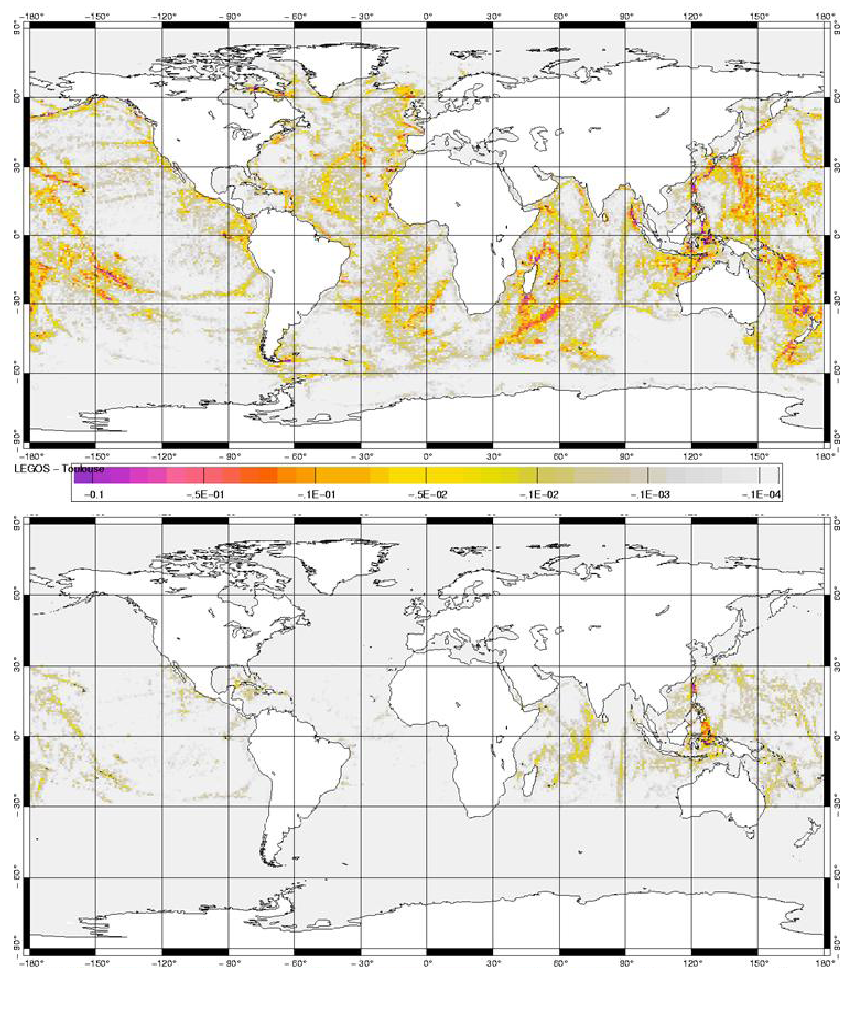
\includegraphics[width=0.90\textwidth]{./TexFiles/Figures/Fig_ZDF_M2_K1_tmx.pdf}
\caption{  \label{Fig_ZDF_M2_K1_tmx} 
(a) M2 and (b) K1 internal wave drag energy from \citet{Carrere_Lyard_GRL03} ($W/m^2$). }
\end{center}  	\end{figure}
%>>>>>>>>>>>>>>>>>>>>>>>>>>>> 
 
% -------------------------------------------------------------------------------------------------------------
%        Indonesian area specific treatment 
% -------------------------------------------------------------------------------------------------------------
\subsection{Indonesian area specific treatment (\np{ln\_zdftmx\_itf})}
\label{ZDF_tmx_itf}

When the Indonesian Through Flow (ITF) area is included in the model domain,
a specific treatment of tidal induced mixing in this area can be used. 
It is activated through the namelist logical \np{ln\_tmx\_itf}, and the user must provide
an input NetCDF file, \ifile{mask\_itf}, which contains a mask array defining the ITF area
where the specific treatment is applied.

When \np{ln\_tmx\_itf}=true, the two key parameters $q$ and $F(z)$ are adjusted following 
the parameterisation developed by \citet{Koch-Larrouy_al_GRL07}:

First, the Indonesian archipelago is a complex geographic region 
with a series of large, deep, semi-enclosed basins connected via 
numerous narrow straits. Once generated, internal tides remain 
confined within this semi-enclosed area and hardly radiate away. 
Therefore all the internal tides energy is consumed within this area. 
So it is assumed that $q = 1$, $i.e.$ all the energy generated is available for mixing.
Note that for test purposed, the ITF tidal dissipation efficiency is a 
namelist parameter (\np{rn\_tfe\_itf}). A value of $1$ or close to is
this recommended for this parameter.

Second, the vertical structure function, $F(z)$, is no more associated
with a bottom intensification of the mixing, but with a maximum of 
energy available within the thermocline. \citet{Koch-Larrouy_al_GRL07} 
have suggested that the vertical distribution of the energy dissipation 
proportional to $N^2$ below the core of the thermocline and to $N$ above. 
The resulting $F(z)$ is:
\begin{equation} \label{Eq_Fz_itf}
F(i,j,k) \sim     \left\{ \begin{aligned}
\frac{q\,\Gamma E(i,j) } {\rho N \, \int N     dz}    \qquad \text{when $\partial_z N < 0$} \\
\frac{q\,\Gamma E(i,j) } {\rho     \, \int N^2 dz}    \qquad \text{when $\partial_z N > 0$}
                      \end{aligned} \right.
\end{equation}

Averaged over the ITF area, the resulting tidal mixing coefficient is $1.5\,cm^2/s$, 
which agrees with the independent estimates inferred from observations. 
Introduced in a regional OGCM, the parameterization improves the water mass 
characteristics in the different Indonesian seas, suggesting that the horizontal 
and vertical distributions of the mixing are adequately prescribed 
\citep{Koch-Larrouy_al_GRL07, Koch-Larrouy_al_OD08a, Koch-Larrouy_al_OD08b}.
Note also that such a parameterisation has a significant impact on the behaviour 
of global coupled GCMs \citep{Koch-Larrouy_al_CD10}.


% ================================================================
			% Vertical diffusion

% ================================================================
% Chapter I/O & Diagnostics
% ================================================================
\chapter{Ouput and Diagnostics (IOM, DIA, TRD, FLO)}
\label{DIA}
\minitoc

\newpage
$\ $\newline    % force a new ligne

% ================================================================
%       Old Model Output 
% ================================================================
\section{Old Model Output (default or \key{dimgout})}
\label{DIA_io_old}

The model outputs are of three types: the restart file, the output listing, 
and the diagnostic output file(s). The restart file is used internally by the code when 
the user wants to start the model with initial conditions defined by a 
previous simulation. It contains all the information that is necessary in 
order for there to be no changes in the model results (even at the computer 
precision) between a run performed with several restarts and the same run 
performed in one step. It should be noted that this requires that the restart file 
contain two consecutive time steps for all the prognostic variables, and 
that it is saved in the same binary format as the one used by the computer 
that is to read it (in particular, 32 bits binary IEEE format must not be used for 
this file). 

The output listing and file(s) are predefined but should be checked 
and eventually adapted to the user's needs. The output listing is stored in 
the $ocean.output$ file. The information is printed from within the code on the 
logical unit $numout$. To locate these prints, use the UNIX command 
"\textit{grep -i numout}" in the source code directory.

By default, diagnostic output files are written in NetCDF format but an IEEE binary output format, called DIMG, can be choosen by defining \key{dimgout}. 

Since version 3.2, when defining \key{iomput}, an I/O server has been added which provides more flexibility in the choice of the fields to be written as well as how the writing work is distributed over the processors in massively parallel computing. The complete description of the use of this I/O server is presented in the next section. 

By default, if neither \key{iomput} nor \key{dimgout} are defined, NEMO produces NetCDF with the old IOIPSL library which has been kept for compatibility and its easy installation. However, the IOIPSL library is quite inefficient on parallel machines and, since version 3.2, many diagnostic options have been added presuming the use of \key{iomput}. The usefulness of the default IOIPSL-based option is expected to reduce with each new release. If \key{iomput} is not defined, output files and content are defined in the \mdl{diawri} module and contain mean (or instantaneous if \key{diainstant} is defined) values over a regular period of nn\_write time-steps (namelist parameter). 

%\gmcomment{                    % start of gmcomment

% ================================================================
% Diagnostics
% ================================================================
\section{Standard model Output (IOM)}
\label{DIA_iom}


Since version 3.2, iomput is the NEMO output interface of choice. It has been designed to be simple to use, flexible and efficient. The two main purposes of iomput are: 
\begin{enumerate}
\item The complete and flexible control of the output files through external XML files adapted by the user from standard templates. 
\item To achieve high performance and scalable output through the optional distribution of all diagnostic output related tasks to dedicated processes. 
\end{enumerate}
The first functionality allows the user to specify, without code changes or recompilation, aspects of the diagnostic output stream, such as:
\begin{itemize}
\item The choice of output frequencies that can be different for each file (including real months and years).
\item The choice of file contents; includes complete flexibility over which data are written in which files (the same data can be written in different files). 
\item The possibility to split output files at a choosen frequency.
\item The possibility to extract a vertical or an horizontal subdomain.
\item The choice of the temporal operation to perform, e.g.: average, accumulate, instantaneous, min, max and once.
\item Control over metadata via a large XML "database" of possible output fields.
\end{itemize}
In addition, iomput allows the user to add the output of any new variable (scalar, 2D or 3D) in the code in a very easy way. All details of iomput functionalities are listed in the following subsections. Examples of the XML files that control the outputs can be found in:
\begin{alltt}
\begin{verbatim}
  NEMOGCM/CONFIG/ORCA2_LIM/EXP00/iodef.xml
  NEMOGCM/CONFIG/SHARED/field_def.xml
  and
  NEMOGCM/CONFIG/SHARED/domain_def.xml.
\end{verbatim}
\end{alltt}

The second functionality targets output performance when running in parallel (\key{mpp\_mpi}). Iomput provides the possibility to specify N dedicated I/O processes (in addition to the NEMO processes) to collect and write the outputs. With an appropriate choice of N by the user, the bottleneck associated with the writing of the output files can be greatly reduced. 

In version 3.6, the iom\_put interface depends on an external code called \href{https://forge.ipsl.jussieu.fr/ioserver/browser/XIOS/branchs/xios-1.0}{XIOS-1.0} (use of revision 618 or higher is required). This new IO server can take advantage of the parallel I/O functionality of NetCDF4 to create a single output file and therefore to bypass the rebuilding phase. Note that writing in parallel into the same NetCDF files requires that your NetCDF4 library is linked to an HDF5 library that has been correctly compiled (i.e. with the configure option $--$enable-parallel). Note that the files created by iomput through XIOS are incompatible with NetCDF3. All post-processsing and visualization tools must therefore be compatible with NetCDF4 and not only NetCDF3.

Even if not using the parallel I/O functionality of NetCDF4, using N dedicated I/O servers, where N is typically much less than the number of NEMO processors, will reduce the number of output files created. This can greatly reduce the post-processing burden usually associated with using large numbers of NEMO processors. Note that for smaller configurations, the rebuilding phase can be avoided, even without a parallel-enabled NetCDF4 library, simply by employing only one dedicated I/O server.

\subsection{XIOS: the IO\_SERVER}

\subsubsection{Attached or detached mode?}

Iomput is based on \href{http://forge.ipsl.jussieu.fr/ioserver/wiki}{XIOS}, the io\_server developed by Yann Meurdesoif from IPSL. The behaviour of the io subsystem is controlled by settings in the external XML files listed above. Key settings in the iodef.xml file are {\tt using\_server} and the {\tt type} tag associated with each defined file. The {\tt using\_server} setting determines whether or not the server will be used in ''attached mode'' (as a library) [{\tt false}] or in ''detached mode'' (as an external executable on N additional, dedicated cpus) [{\tt true}]. The ''attached mode'' is simpler to use but much less efficient for massively parallel applications. The type of each file can be either ''multiple\_file'' or ''one\_file''.

In attached mode and if the type of file is ''multiple\_file'', then each NEMO process will also act as an IO server and produce its own set of output files. Superficially, this emulates the standard behaviour in previous versions, However, the subdomain written out by each process does not correspond to the {\tt jpi x jpj x jpk} domain actually computed by the process (although it may if {\tt jpni=1}). Instead each process will have collected and written out a number of complete longitudinal strips. If the ''one\_file'' option is chosen then all processes will collect their longitudinal strips and write (in parallel) to a single output file. 

In detached mode and if the type of file is ''multiple\_file'', then each stand-alone XIOS process will collect data for a range of complete longitudinal strips and write to its own set of output files. If the ''one\_file'' option is chosen then all XIOS processes will collect their longitudinal strips and write (in parallel) to a single output file. Note running in detached mode requires launching a Multiple Process Multiple Data (MPMD) parallel job. The following subsection provides a typical example but the syntax will vary in different MPP environments.

\subsubsection{Number of cpu used by XIOS in detached mode}

The number of cores used by the XIOS is specified when launching the model. The number of cores dedicated to XIOS should be from ~1/10 to ~1/50 of the number or cores dedicated to NEMO. Some manufacturers suggest using O($\sqrt{N}$) dedicated IO processors for N processors but this is a general recommendation and not specific to NEMO. It is difficult to provide precise recommendations because the optimal choice will depend on the particular hardware properties of the target system (parallel filesystem performance, available memory, memory bandwidth etc.) and the volume and frequency of data to be created. Here is an example of 2 cpus for the io\_server and 62 cpu for nemo using mpirun:

\texttt{ mpirun -np 62 ./nemo.exe : -np 2 ./xios\_server.exe }

\subsubsection{Control of XIOS: the XIOS context in iodef.xml}

As well as the {\tt using\_server} flag, other controls on the use of XIOS are set in the XIOS context in iodef.xml. See the XML basics section below for more details on XML syntax and rules.

\begin{tabular}{|p{4cm}|p{6.0cm}|p{2.0cm}|}
   \hline
   variable name & 
   description & 
   example \\ 
   \hline   
   \hline
   buffer\_size & 
   buffer size used by XIOS to send data from NEMO to XIOS. Larger is more efficient. Note that needed/used buffer sizes are summarized at the end of the job & 
   25000000 \\ 
   \hline   
   buffer\_server\_factor\_size & 
   ratio between NEMO and XIOS buffer size. Should be 2. & 
   2 \\ 
   \hline
   info\_level & 
   verbosity level (0 to 100) & 
   0 \\ 
   \hline
   using\_server & 
   activate attached(false) or detached(true) mode & 
   true \\ 
   \hline
   using\_oasis & 
   XIOS is used with OASIS(true) or not (false) & 
   false \\ 
   \hline
   oasis\_codes\_id & 
   when using oasis, define the identifier of NEMO in the namcouple. Note that the identifier of XIOS is xios.x & 
   oceanx \\ 
   \hline   
\end{tabular}


\subsection{Practical issues}

\subsubsection{Installation}

As mentioned, XIOS is supported separately and must be downloaded and compiled before it can be used with NEMO. See the installation guide on the \href{http://forge.ipsl.jussieu.fr/ioserver/wiki}{XIOS} wiki for help and guidance. NEMO will need to link to the compiled XIOS library. The 
\href{http://www.nemo-ocean.eu/Using-NEMO/User-Guides/Basics/XIOS-IO-server-installation-and-use}{XIOS with NEMO} guide provides an example illustration of how this can be achieved.

\subsubsection{Add your own outputs}

It is very easy to add your own outputs with iomput. Many standard fields and diagnostics are already prepared (i.e., steps 1 to 3 below have been done) and simply need to be activated by including the required output in a file definition in iodef.xml (step 4). To add new output variables, all 4 of the following steps must be taken.
\begin{description}
\item[1.] in NEMO code, add a \\
\texttt{      CALL iom\_put( 'identifier', array ) } \\
where you want to output a 2D or 3D array.

\item[2.] If necessary, add \\
\texttt{   USE iom\ \ \ \ \ \ \ \ \ \ \ \ ! I/O manager library }  \\
to the list of used modules in the upper part of your module. 

\item[3.] in the field\_def.xml file, add the definition of your variable using the same identifier you used in the f90 code (see subsequent sections for a details of the XML syntax and rules). For example:
\vspace{-20pt}
\begin{alltt}  {{\scriptsize
\begin{verbatim}
   <field_definition>
      <!-- T grid -->

     <field_group id="grid_T" grid_ref="grid_T_3D">
      ...
      <field id="identifier" long_name="blabla" ... />   
      ...
   </field_definition> 
\end{verbatim}
}}\end{alltt} 
Note your definition must be added to the field\_group whose reference grid is consistent with the size of the array passed to iomput. The grid\_ref attribute refers to definitions set in iodef.xml which, in turn, reference grids and axes either defined in the code (iom\_set\_domain\_attr and iom\_set\_axis\_attr in iom.F90) or defined in the domain\_def.xml file. E.g.:
\vspace{-20pt}
\begin{alltt}  {{\scriptsize
\begin{verbatim}
     <grid id="grid_T_3D" domain_ref="grid_T" axis_ref="deptht"/>
\end{verbatim}
}}\end{alltt} 
Note, if your array is computed within the surface module each nn\_fsbc time\_step, 
add the field definition within the field\_group defined with the id ''SBC'': $<$field\_group id=''SBC''...$>$ which has been defined with the correct frequency of operations (iom\_set\_field\_attr in iom.F90)

\item[4.] add your field in one of the output files defined in iodef.xml (again see subsequent sections for syntax and rules)   \\
\vspace{-20pt}
\begin{alltt}  {{\scriptsize
\begin{verbatim}
   <file id="file1" .../>   
      ...
      <field field_ref="identifier" />   
      ...
   </file>   
\end{verbatim}
}}\end{alltt} 

\end{description}
\subsection{XML fundamentals}

\subsubsection{ XML basic rules}

XML tags begin with the less-than character ("$<$") and end with the greater-than character (''$>$''). 
You use tags to mark the start and end of elements, which are the logical units of information 
in an XML document. In addition to marking the beginning of an element, XML start tags also 
provide a place to specify attributes. An attribute specifies a single property for an element, 
using a name/value pair, for example: $<$a b="x" c="y" b="z"$>$ ... $<$/a$>$.
See \href{http://www.xmlnews.org/docs/xml-basics.html}{here} for more details.

\subsubsection{Structure of the xml file used in NEMO}

The XML file used in XIOS is structured by 7 families of tags: context, axis, domain, grid, field, file and variable. Each tag family has hierarchy of three flavors (except for context):
\\
\begin{tabular}{|p{3.0cm}|p{4.5cm}|p{4.5cm}|}
   \hline
   flavor &
   description &
   example \\
   \hline
   \hline
   root &
   declaration of the root element that can contain element groups or elements &
   {\scriptsize \verb? < file_definition ... >?} \\
   \hline
   group &
   declaration of a group element that can contain element groups or elements &
   {\scriptsize \verb? < file_group ... >?} \\
   \hline
   element &
   declaration of an element that can contain elements &
   {\scriptsize \verb? < file ... >?} \\
   \hline
\end{tabular}
\\

Each element may have several attributes. Some attributes are mandatory, other are optional but have a default value and other are are completely optional. Id is a special attribute used to identify an element or a group of elements. It must be unique for a kind of element. It is optional, but no reference to the corresponding element can be done if it is not defined.

The XML file is split into context tags that are used to isolate IO definition from different codes or different parts of a code. No interference is possible between 2 different contexts. Each context has its own calendar and an associated timestep. In NEMO, we used the following contexts (that can be defined in any order):\\
\\
\begin{tabular}{|p{3.0cm}|p{4.5cm}|p{4.5cm}|}
   \hline
   context &
   description &
   example \\
   \hline
   \hline
   context xios &
   context containing information for XIOS &
   {\scriptsize \verb? <context id="xios" ...  ?} \\
   \hline
   context nemo &
   context containing IO information for NEMO (mother grid when using AGRIF) &
   {\scriptsize \verb? <context id="nemo" ... ?} \\
   \hline
   context 1\_nemo &
   context containing IO information for NEMO child grid 1 (when using AGRIF) &
   {\scriptsize \verb? <context id="1_nemo" ...  ?} \\
   \hline
   context n\_nemo &
   context containing IO information for NEMO child grid n (when using AGRIF) &
   {\scriptsize \verb? <context id="n_nemo" ...  ?} \\
   \hline
\end{tabular}
\\

\noindent The xios context contains only 1 tag:
\\
\begin{tabular}{|p{3.0cm}|p{4.5cm}|p{4.5cm}|}
   \hline
   context tag &
   description &
   example \\
   \hline
   \hline
   variable\_definition &
   define variables needed by XIOS. This can be seen as a kind of namelist for XIOS. &
   {\scriptsize \verb? <variable_definition ... ?} \\
   \hline
\end{tabular}
\\

\noindent Each context tag related to NEMO (mother or child grids) is divided into 5 parts (that can be defined in any order):\\
\\
\begin{tabular}{|p{3.0cm}|p{4.5cm}|p{4.5cm}|}
   \hline
   context tag &
   description &
   example \\
   \hline
   \hline
   field\_definition &
   define all variables that can potentially be outputted &
   {\scriptsize \verb? <field_definition ... ?} \\
   \hline
   file\_definition &
   define the netcdf files to be created and the variables they will contain &
   {\scriptsize \verb? <file_definition ... ?} \\
   \hline
   axis\_definition &
   define vertical axis &
   {\scriptsize \verb? <axis_definition ... ?} \\
   \hline
   domain\_definition &
   define the horizontal grids &
   {\scriptsize \verb? <domain_definition ... ?} \\
   \hline
   grid\_definition &
   define the 2D and 3D grids (association of an axis and a domain) &
   {\scriptsize \verb? <grid_definition ... ?} \\
   \hline
\end{tabular}
\\

\subsubsection{Nesting XML files}

The XML file can be split in different parts to improve its readability and facilitate its use. The inclusion of XML files into the main XML file can be done through the attribute src: \\
{\scriptsize \verb? <context src="./nemo_def.xml" /> ?}\\
 
\noindent In NEMO, by default, the field and domain definition is done in 2 separate files:
{\scriptsize \tt
\begin{verbatim}
NEMOGCM/CONFIG/SHARED/field_def.xml
and
NEMOGCM/CONFIG/SHARED/domain_def.xml 
\end{verbatim}
}
\noindent that are included in the main iodef.xml file through the following commands: \\
{\scriptsize \verb? <field_definition src="./field_def.xml" /> ? \\
\verb? <domain_definition src="./domain_def.xml" /> ? }


\subsubsection{Use of inheritance}

XML extensively uses the concept of inheritance. XML has a tree based structure with a parent-child oriented relation: all children inherit attributes from parent, but an attribute defined in a child replace the inherited attribute value. Note that the special attribute ''id'' is never inherited.  \\
\\
example 1: Direct inheritance.
\vspace{-20pt}
\begin{alltt}  {{\scriptsize    
\begin{verbatim}
   <field_definition operation="average" >
     <field id="sst"                    />   <!-- averaged      sst --> 
     <field id="sss" operation="instant"/>   <!-- instantaneous sss --> 
   </field_definition> 
\end{verbatim}
}}\end{alltt} 

The field ''sst'' which is part (or a child) of the field\_definition will inherit the value ''average'' 
of the attribute ''operation'' from its parent. Note that a child can overwrite 
the attribute definition inherited from its parents. In the example above, the field ''sss'' will 
for example output instantaneous values instead of average values. \\
\\
example 2: Inheritance by reference.
\vspace{-20pt}
\begin{alltt}  {{\scriptsize
\begin{verbatim}
   <field_definition>
     <field id="sst" long_name="sea surface temperature" />   
     <field id="sss" long_name="sea surface salinity"    />  
   </field_definition>      

   <file_definition>
     <file id="myfile" output_freq="1d" />   
       <field field_ref="sst"                            />  <!-- default def -->
       <field field_ref="sss" long_name="my description" />  <!-- overwrite   -->
     </file>   
   </file_definition> 
\end{verbatim}
}}\end{alltt} 
Inherit (and overwrite, if needed) the attributes of a tag you are refering to.

\subsubsection{Use of Groups}

Groups can be used for 2 purposes. Firstly, the group can be used to define common attributes to be shared by the elements of the group through inheritance. In the following example, we define a group of field that will share a common grid ''grid\_T\_2D''. Note that for the field ''toce'', we overwrite the grid definition inherited from the group by ''grid\_T\_3D''.
\vspace{-20pt}
\begin{alltt}  {{\scriptsize
\begin{verbatim}
   <field_group id="grid_T" grid_ref="grid_T_2D">
    <field id="toce" long_name="temperature"             unit="degC" grid_ref="grid_T_3D"/>
    <field id="sst"  long_name="sea surface temperature" unit="degC"                     />
    <field id="sss"  long_name="sea surface salinity"    unit="psu"                      />
    <field id="ssh"  long_name="sea surface height"      unit="m"                        />
         ...
\end{verbatim}
}}\end{alltt} 

Secondly, the group can be used to replace a list of elements. Several examples of groups of fields are proposed at the end of the file {\tt CONFIG/SHARED/field\_def.xml}. For example, a short list of the usual variables related to the U grid:
\vspace{-20pt}
\begin{alltt}  {{\scriptsize
\begin{verbatim}
   <field_group id="groupU" >
    <field field_ref="uoce"  />
    <field field_ref="suoce" />
    <field field_ref="utau"  />
   </field_group>
\end{verbatim}
}}\end{alltt} 
that can be directly included in a file through the following syntax:
\vspace{-20pt}
\begin{alltt}  {{\scriptsize
\begin{verbatim}
   <file id="myfile_U" output_freq="1d" />   
    <field_group group_ref="groupU"/>  
    <field field_ref="uocetr_eff"  />  <!-- add another field -->
   </file>   
\end{verbatim}
}}\end{alltt} 

\subsection{Detailed functionalities }

The file {\tt NEMOGCM/CONFIG/ORCA2\_LIM/iodef\_demo.xml} provides several examples of the use of the new functionalities offered by the XML interface of XIOS. 

\subsubsection{Define horizontal subdomains}
Horizontal subdomains are defined through the attributs zoom\_ibegin, zoom\_jbegin, zoom\_ni, zoom\_nj of the tag family domain. It must therefore be done in the domain part of the XML file. For example, in {\tt CONFIG/SHARED/domain\_def.xml}, we provide the following example of a definition of a 5 by 5 box with the bottom left corner at point (10,10).
\vspace{-20pt}
\begin{alltt}  {{\scriptsize
\begin{verbatim}
   <domain_group id="grid_T">
    <domain id="myzoom" zoom_ibegin="10" zoom_jbegin="10" zoom_ni="5" zoom_nj="5" />
\end{verbatim}
}}\end{alltt} 
The use of this subdomain is done through the redefinition of the attribute domain\_ref of the tag family field. For example:
\vspace{-20pt}
\begin{alltt}  {{\scriptsize
\begin{verbatim}
   <file id="myfile_vzoom" output_freq="1d" >
      <field field_ref="toce" domain_ref="myzoom"/>
   </file>
\end{verbatim}
}}\end{alltt} 
Moorings are seen as an extrem case corresponding to a 1 by 1 subdomain. The Equatorial section, the TAO, RAMA and PIRATA moorings are alredy registered in the code and can therefore be outputted without taking care of their (i,j) position in the grid. These predefined domains can be activated by the use of specific domain\_ref: ''EqT'', ''EqU'' or ''EqW'' for the equatorial sections and the mooring position for TAO, RAMA and PIRATA followed by ''T'' (for example: ''8s137eT'', ''1.5s80.5eT'' ...)
\vspace{-20pt}
\begin{alltt}  {{\scriptsize
\begin{verbatim}
   <file id="myfile_vzoom" output_freq="1d" >
      <field field_ref="toce" domain_ref="0n180wT"/>
   </file>
\end{verbatim}
}}\end{alltt} 
Note that if the domain decomposition used in XIOS cuts the subdomain in several parts and if you use the ''multiple\_file'' type for your output files, you will endup with several files you will need to rebuild using unprovided tools (like ncpdq and ncrcat, \href{http://nco.sourceforge.net/nco.html#Concatenation}{see nco manual}). We are therefore advising to use the ''one\_file'' type in this case.

\subsubsection{Define vertical zooms}
Vertical zooms are defined through the attributs zoom\_begin and zoom\_end of the tag family axis. It must therefore be done in the axis part of the XML file. For example, in NEMOGCM/CONFIG/ORCA2\_LIM/iodef\_demo.xml, we provide the following example:
\vspace{-20pt}
\begin{alltt}  {{\scriptsize
\begin{verbatim}
   <axis_group id="deptht" long_name="Vertical T levels" unit="m" positive="down" >
      <axis id="deptht" />
      <axis id="deptht_myzoom" zoom_begin="1" zoom_end="10" />
\end{verbatim}
}}\end{alltt} 
The use of this vertical zoom is done through the redefinition of the attribute axis\_ref of the tag family field. For example:
\vspace{-20pt}
\begin{alltt}  {{\scriptsize
\begin{verbatim}
   <file id="myfile_hzoom" output_freq="1d" >
      <field field_ref="toce" axis_ref="deptht_myzoom"/>
   </file>
\end{verbatim}
}}\end{alltt} 

\subsubsection{Control of the output file names}

The output file names are defined by the attributs ''name'' and ''name\_suffix'' of the tag family file. for example:
\vspace{-20pt}
\begin{alltt}  {{\scriptsize
\begin{verbatim}
   <file_group id="1d" output_freq="1d" name="myfile_1d" > 
      <file id="myfileA" name_suffix="_AAA" > <!-- will create file "myfile_1d_AAA"  -->
         ...
      </file>
      <file id="myfileB" name_suffix="_BBB" > <!-- will create file "myfile_1d_BBB" -->
         ...
      </file>
   </file_group>
\end{verbatim}
}}\end{alltt} 
However it is often very convienent to define the file name with the name of the experiment, the output file frequency and the date of the beginning and the end of the simulation (which are informations stored either in the namelist or in the XML file). To do so, we added the following rule: if the id of the tag file is ''fileN''(where N = 1 to 999 on 1 to 3 digits) or one of the predefined sections or moorings (see next subsection), the following part of the name and the name\_suffix (that can be inherited) will be automatically replaced by:\\
\\
\begin{tabular}{|p{4cm}|p{8cm}|}
   \hline
   \centering placeholder string & automatically  replaced by \\
   \hline
   \hline
   \centering @expname@ &
   the experiment name (from cn\_exp in the namelist) \\
   \hline
   \centering @freq@ &
   output frequency (from attribute output\_freq) \\
   \hline
   \centering @startdate@  &
   starting date of the simulation (from nn\_date0 in the restart or the namelist). \verb?yyyymmdd? format \\
   \hline
   \centering @startdatefull@  & 
   starting date of the simulation (from nn\_date0 in the restart or the namelist). \verb?yyyymmdd_hh:mm:ss? format \\
   \hline
   \centering @enddate@  &
   ending date of the simulation (from nn\_date0 and nn\_itend in the namelist). \verb?yyyymmdd? format \\
   \hline
   \centering @enddatefull@  & 
   ending date of the simulation (from nn\_date0 and nn\_itend in the namelist). \verb?yyyymmdd_hh:mm:ss? format \\
   \hline
\end{tabular}\\
\\

\noindent For example, 
{{\scriptsize
\begin{verbatim}
   <file id="myfile_hzoom" name="myfile_@expname@_@startdate@_freq@freq@" output_freq="1d" >
\end{verbatim}
}}
\noindent with the namelist:
{{\scriptsize
\begin{verbatim}
   cn_exp      =  "ORCA2"
   nn_date0    =  19891231
   ln_rstart   = .false.
\end{verbatim}
}}
\noindent will give the following file name radical:
{{\scriptsize
\begin{verbatim}
   myfile_ORCA2_19891231_freq1d 
\end{verbatim}
}}

\subsubsection{Other controls of the xml attributes from NEMO}

The values of some attributes are defined by subroutine calls within NEMO (calls to iom\_set\_domain\_attr, iom\_set\_axis\_attr and iom\_set\_field\_attr in iom.F90). Any definition given in the xml file will be overwritten. By convention, these attributes are defined to ''auto'' (for string) or ''0000'' (for integer) in the xml file (but this is not necessary). 

Here is the list of these attributes:\\
\\
\begin{tabular}{|l|c|c|c|}
   \hline
 \multicolumn{2}{|c|}{tag ids affected by automatic           }  & name      & attribute value \\
  \multicolumn{2}{|c|}{definition of some of their attributes }  & attribute  &        \\
   \hline
   \hline
    \multicolumn{2}{|c|}{field\_definition} & freq\_op & \np{rn\_rdt} \\
   \hline
    \multicolumn{2}{|c|}{SBC}               & freq\_op & \np{rn\_rdt} $\times$ \np{nn\_fsbc}  \\
   \hline
    \multicolumn{2}{|c|}{ptrc\_T}           & freq\_op & \np{rn\_rdt} $\times$ \np{nn\_dttrc} \\
   \hline
    \multicolumn{2}{|c|}{diad\_T}           & freq\_op & \np{rn\_rdt} $\times$ \np{nn\_dttrc} \\
   \hline
    \multicolumn{2}{|c|}{EqT, EqU, EqW} & jbegin, ni,      & according to the grid    \\
    \multicolumn{2}{|c|}{                         } & name\_suffix &                                      \\
   \hline
   \multicolumn{2}{|c|}{TAO, RAMA and PIRATA moorings} & zoom\_ibegin, zoom\_jbegin, & according to the grid    \\
    \multicolumn{2}{|c|}{                                                       } & name\_suffix &                                      \\
   \hline
\end{tabular}

\subsubsection{Advanced use of XIOS functionalities}

\subsection{XML reference tables}
\label{IOM_xmlref}

(1) Simple computation: directly define the computation when refering to the variable in the file definition.

\vspace{-20pt}
\begin{alltt}  {{\scriptsize    
\begin{verbatim}
 <field field\_ref="sst"  name="tosK"  unit="degK" > sst + 273.15 </field>
 <field field\_ref="taum" name="taum2" unit="N2/m4" long\_name="square of wind stress module" > taum * taum </field>
 <field field\_ref="qt"   name="stupid\_check" > qt - qsr - qns </field>
\end{verbatim}
}}\end{alltt} 

(2) Simple computation: define a new variable and use it in the file definition.

in field\_definition:
\vspace{-20pt}
\begin{alltt}  {{\scriptsize    
\begin{verbatim}
 <field id="sst2" long\_name="square of sea surface temperature" unit="degC2" >  sst * sst </field >
\end{verbatim}
}}\end{alltt} 
in file\_definition:
\vspace{-20pt}
\begin{alltt}  {{\scriptsize    
\begin{verbatim}
 <field field\_ref="sst2" > sst2 </field>
\end{verbatim}
}}\end{alltt} 
Note that in this case, the following syntaxe $<$field field\_ref="sst2" /$>$ is not working as sst2 won't be evaluated.

(3) Change of variable precision:

\vspace{-20pt}
\begin{alltt}  {{\scriptsize    
\begin{verbatim}
     <!-- force to keep real 8 -->
 <field field\_ref="sst" name="tos\_r8" prec="8" />
      <!-- integer 2  with add\_offset and scale\_factor attributes -->
 <field field\_ref="sss" name="sos\_i2" prec="2" add\_offset="20." scale\_factor="1.e-3" />
\end{verbatim}
}}\end{alltt} 
Note that, then the code is crashing, writting real4 variables forces a numerical convection from real8 to real4 which will create an internal error in NetCDF and will avoid the creation of the output files. Forcing double precision outputs with prec="8" (for example in the field\_definition) will avoid this problem.

(4) add user defined attributes:

\vspace{-20pt}
\begin{alltt}  {{\scriptsize    
\begin{verbatim}
      <file\_group id="1d" output\_freq="1d" output\_level="10" enabled=".TRUE."> <!-- 1d files --> 
	<file id="file1" name\_suffix="\_grid\_T" description="ocean T grid variables" >
	  <field field\_ref="sst" name="tos" >
	    <variable id="my\_attribute1" type="string"  > blabla </variable>
	    <variable id="my\_attribute2" type="integer" > 3      </variable>
	    <variable id="my\_attribute3" type="float"   > 5.0    </variable>
	  </field>
	  <variable id="my\_global\_attribute" type="string" > blabla\_global </variable>
       </file>
     </file\_group> 
\end{verbatim}
}}\end{alltt} 

(5) use of the ``@'' function: example 1, weighted temporal average

 - define a new variable in field\_definition
\vspace{-20pt}
\begin{alltt}  {{\scriptsize    
\begin{verbatim}
 <field id="toce\_e3t" long\_name="temperature * e3t" unit="degC*m" grid\_ref="grid\_T\_3D" > toce * e3t </field >
\end{verbatim}
}}\end{alltt}
 - use it when defining your file.  
\vspace{-20pt}
\begin{alltt}  {{\scriptsize    
\begin{verbatim}
<file\_group id="5d" output\_freq="5d"  output\_level="10" enabled=".TRUE." >  <!-- 5d files -->  
 <file id="file1" name\_suffix="\_grid\_T" description="ocean T grid variables" >
  <field field\_ref="toce" operation="instant" freq\_op="5d" > @toce\_e3t / @e3t </field>
 </file>
</file\_group> 
\end{verbatim}
}}\end{alltt}
The freq\_op="5d" attribute is used to define the operation frequency of the ``@'' function: here 5 day. The temporal operation done by the ``@'' is the one defined in the field definition: here we use the default, average. So, in the above case, @toce\_e3t will do the 5-day mean of toce*e3t. Operation="instant" refers to the temporal operation to be performed on the field''@toce\_e3t / @e3t'': here the temporal average is alreday done by the ``@'' function so we just use instant to do the ratio of the 2 mean values. field\_ref="toce" means that attributes not explicitely defined, are inherited from toce field. Note that in this case, freq\_op must be equal to the file output\_freq.

(6) use of the ``@'' function: example 2, monthly SSH standard deviation

 - define a new variable in field\_definition
\vspace{-20pt}
\begin{alltt}  {{\scriptsize    
\begin{verbatim}
 <field id="ssh2" long\_name="square of sea surface temperature" unit="degC2" >  ssh * ssh </field >
\end{verbatim}
}}\end{alltt} 
 - use it when defining your file.  
\vspace{-20pt}
\begin{alltt}  {{\scriptsize    
\begin{verbatim}
<file\_group id="1m" output\_freq="1m"  output\_level="10" enabled=".TRUE." >  <!-- 1m files -->  
 <file id="file1" name\_suffix="\_grid\_T" description="ocean T grid variables" >
  <field field\_ref="ssh" name="sshstd" long\_name="sea\_surface\_temperature\_standard\_deviation" operation="instant" freq\_op="1m" > sqrt( @ssh2 - @ssh * @ssh ) </field>
 </file>
</file\_group> 
\end{verbatim}
}}\end{alltt}
The freq\_op="1m" attribute is used to define the operation frequency of the ``@'' function: here 1 month. The temporal operation done by the ``@'' is the one defined in the field definition: here we use the default, average. So, in the above case, @ssh2 will do the monthly mean of ssh*ssh. Operation="instant" refers to the temporal operation to be performed on the field ''sqrt( @ssh2 - @ssh * @ssh )'': here the temporal average is alreday done by the ``@'' function so we just use instant. field\_ref="ssh" means that attributes not explicitely defined, are inherited from ssh field. Note that in this case, freq\_op must be equal to the file output\_freq.

(7) use of the ``@'' function: example 3, monthly average of SST diurnal cycle

 - define 2 new variables in field\_definition
\vspace{-20pt}
\begin{alltt}  {{\scriptsize    
\begin{verbatim}
 <field id="sstmax" field\_ref="sst" long\_name="max of sea surface temperature" operation="maximum" />
 <field id="sstmin" field\_ref="sst" long\_name="min of sea surface temperature" operation="minimum" />
\end{verbatim}
}}\end{alltt} 
 - use these 2 new variables when defining your file.  
\vspace{-20pt}
\begin{alltt}  {{\scriptsize    
\begin{verbatim}
<file\_group id="1m" output\_freq="1m"  output\_level="10" enabled=".TRUE." >  <!-- 1m files -->  
 <file id="file1" name\_suffix="\_grid\_T" description="ocean T grid variables" >
  <field field\_ref="sst" name="sstdcy" long\_name="amplitude of sst diurnal cycle" operation="average" freq\_op="1d" > @sstmax - @sstmin </field>
 </file>
</file\_group> 
\end{verbatim}
}}\end{alltt}
The freq\_op="1d" attribute is used to define the operation frequency of the ``@'' function: here 1 day. The temporal operation done by the ``@'' is the one defined in the field definition: here maximum for sstmax and minimum for sstmin. So, in the above case, @sstmax will do the daily max and @sstmin the daily min. Operation="average" refers to the temporal operation to be performed on the field ``@sstmax - @sstmin'': here monthly mean (of daily max - daily min of the sst). field\_ref="sst" means that attributes not explicitely defined, are inherited from sst field.



\subsubsection{Tag list}

\begin{longtable}{|p{2.2cm}|p{2.5cm}|p{3.5cm}|p{2.2cm}|p{1.6cm}|}
   \hline
   tag name & 
   description & 
   accepted attribute & 
   child of &
   parent of \endhead
   \hline   
   simulation & 
   this tag is the root tag which encapsulates all the content of the xml file &
   none &
   none &
   context \\
   \hline   
   context &
   encapsulates parts of the xml file dedicated to different codes or different parts of a code &
   id (''xios'', ''nemo'' or ''n\_nemo'' for the nth AGRIF zoom), src, time\_origin &
   simulation &
   all root tags: ... \_definition \\
   \hline   
   \hline   
   field\_definition &
   encapsulates the definition of all the fields that can potentially be outputted &
   axis\_ref, default\_value, domain\_ref, enabled, grid\_ref, level, operation, prec, src &
   context &
   field or field\_group \\
   \hline   
   field\_group &
   encapsulates a group of fields &
   axis\_ref, default\_value, domain\_ref, enabled, group\_ref, grid\_ref, id, level, operation, prec, src &
   field\_definition, field\_group, file &
   field or field\_group \\
   \hline   
   field &
   define a specific field &
   axis\_ref, default\_value, domain\_ref, enabled, field\_ref, grid\_ref, id, level, long\_name, name, operation, prec, standard\_name, unit &
   field\_definition, field\_group, file &
   none \\
   \hline   
   \hline   
   file\_definition & 
   encapsulates the definition of all the files that will be outputted &
   enabled, min\_digits, name, name\_suffix, output\_level, split\_freq\_format, split\_freq, sync\_freq, type, src &
   context & 
   file or file\_group \\
   \hline   
   file\_group & 
   encapsulates a group of files that will be outputted &
   enabled, description, id, min\_digits, name, name\_suffix, output\_freq, output\_level, split\_freq\_format, split\_freq, sync\_freq, type, src &
   file\_definition, file\_group & 
   file or file\_group \\
   \hline   
   file & 
   define the contents of a file to be outputted &
   enabled, description, id, min\_digits, name, name\_suffix, output\_freq, output\_level, split\_freq\_format, split\_freq, sync\_freq, type, src &
   file\_definition, file\_group & 
   field \\
   \hline   
   axis\_definition & 
   define all the vertical axis potentially used by the variables &
   src &
   context &  
   axis\_group, axis \\
   \hline   
   axis\_group & 
   encapsulates a group of vertical axis &
   id, lon\_name, positive, src, standard\_name, unit, zoom\_begin, zoom\_end, zoom\_size &
   axis\_definition, axis\_group & 
   axis\_group, axis \\
   \hline   
   axis & 
   define a vertical axis &
   id, lon\_name, positive, src, standard\_name, unit, zoom\_begin, zoom\_end, zoom\_size &
   axis\_definition, axis\_group  & 
   none \\
   \hline   
   \hline   
   domain\_\-definition & 
   define all the horizontal domains potentially used by the variables &
   src &
   context & 
   domain\_\-group, domain \\
   \hline   
   domain\_group & 
   encapsulates a group of horizontal domains &
   id, lon\_name, src, zoom\_ibegin, zoom\_jbegin, zoom\_ni, zoom\_nj &
   domain\_\-definition, domain\_group & 
   domain\_\-group, domain \\
   \hline   
   domain & 
   define an horizontal domain &
   id, lon\_name, src, zoom\_ibegin, zoom\_jbegin, zoom\_ni, zoom\_nj &
   domain\_\-definition, domain\_group & 
   none \\
   \hline   
   \hline   
   grid\_definition & 
   define all the grid (association of a domain and/or an axis) potentially used by the variables &
   src &
   context & 
   grid\_group, grid \\
   \hline   
   grid\_group & 
   encapsulates a group of grids &
   id, domain\_ref, axis\_ref &
   grid\_definition, grid\_group & 
   grid\_group, grid \\
   \hline   
   grid & 
   define a grid &
   id, domain\_ref, axis\_ref &
   grid\_definition, grid\_group & 
   none \\
   \hline   
\end{longtable}


\subsubsection{Attributes list}

\begin{longtable}{|p{2.2cm}|p{4cm}|p{3.8cm}|p{2cm}|}
   \hline
   attribute name & 
   description & 
   example & 
   accepted by \endhead
   \hline   
   axis\_ref & 
   refers to the id of a vertical axis & 
   axis\_ref="deptht" & 
   field, grid families \\ 
   \hline   
   enabled & 
   switch on/off the output of a field or a file & 
   enabled=".TRUE." & 
   field, file families \\ 
   \hline   
   default\_value & 
   missing\_value definition & 
   default\_value="1.e20" & 
   field family \\ 
   \hline   
   description & 
   just for information, not used & 
   description="ocean T grid variables" & 
   all tags \\ 
   \hline   
   domain\_ref & 
   refers to the id of a domain & 
   domain\_ref="grid\_T" & 
   field or grid families \\ 
   \hline   
   field\_ref & 
   id of the field we want to add in a file & 
   field\_ref="toce" & 
   field \\ 
   \hline   
   grid\_ref & 
   refers to the id of a grid & 
   grid\_ref="grid\_T\_2D" & 
   field family \\ 
   \hline   
   group\_ref & 
   refer to a group of variables & 
   group\_ref="mooring" & 
   field\_group \\ 
   \hline   
   id & 
   allow to identify a tag & 
   id="nemo" &
   accepted by all tags except simulation \\ 
   \hline   
   level & 
   output priority of a field: 0 (high) to 10 (low)& 
   level="1" & 
   field family \\ 
   \hline   
   long\_name & 
   define the long\_name attribute in the NetCDF file & 
   long\_name="Vertical T levels" & 
   field \\ 
   \hline   
   min\_digits & 
   specify the minimum of digits used in the core number in the name of the NetCDF file & 
   min\_digits="4" & 
   file family \\ 
   \hline   
   name & 
   name of a variable or a file. If the name of a file is undefined, its id is used as a name & 
   name="tos" & 
   field or file families \\ 
   \hline   
   name\_suffix & 
   suffix to be inserted after the name and before the cpu number and the ''.nc'' termination of a file & 
   name\_suffix="\_myzoom" & 
   file family \\ 
   \hline   
   attribute name & 
   description & 
   example & 
   accepted by \\ 
   \hline   
   \hline   
   operation & 
   type of temporal operation: average, accumulate, instantaneous, min, max and once & 
   operation="average" & 
   field family \\ 
   \hline   
   output\_freq & 
   operation frequency. units can be ts (timestep), y, mo, d, h, mi, s. & 
   output\_freq="1d12h" & 
   field family \\ 
   \hline   
   output\_level & 
   output priority of variables in a file: 0 (high) to 10 (low). All variables listed in the file with a level smaller or equal to output\_level will be output. Other variables won't be output even if they are listed in the file. &  
   output\_level="10"& 
   file family \\ 
   \hline   
   positive & 
   convention used for the orientation of vertival axis (positive downward in \NEMO). & 
   positive="down" & 
   axis family \\ 
   \hline   
   prec & 
   output precision: real 4 or real 8 & 
   prec="4" & 
   field family \\ 
   \hline   
   split\_freq & 
   frequency at which to temporally split output files. Units can be ts (timestep), y, mo, d, h, mi, s. Useful for long runs to prevent over-sized output files.& 
   split\_freq="1mo" & 
   file family \\ 
   \hline   
   split\_freq\-\_format & 
   date format used in the name of temporally split output files. Can be specified 
   using the following syntaxes: \%y, \%mo, \%d, \%h \%mi and \%s & 
   split\_freq\_format= "\%y\%mo\%d" & 
   file family \\ 
   \hline   
   src & 
   allow to include a file & 
   src="./field\_def.xml" & 
   accepted by all tags except simulation \\ 
   \hline   
   standard\_name & 
   define the standard\_name attribute in the NetCDF file & 
   standard\_name= "Eastward\_Sea\_Ice\_Transport" & 
   field \\ 
   \hline   
   sync\_freq & 
   NetCDF file synchronization frequency (update of the time\_counter). units can be ts (timestep), y, mo, d, h, mi, s. & 
   sync\_freq="10d" & 
   file family \\ 
   \hline   
   attribute name & 
   description & 
   example & 
   accepted by \\ 
   \hline   
   \hline   
   time\_origin & 
   specify the origin of the time counter & 
   time\_origin="1900-01-01 00:00:00"& 
   context \\ 
   \hline   
   type (1)& 
   specify if the output files are to be split spatially (multiple\_file) or not (one\_file) & 
   type="multiple\_file" & 
   file familly \\ 
   \hline   
   type (2)& 
   define the type of a variable tag & 
   type="boolean" & 
   variable \\ 
   \hline   
   unit & 
   unit of a variable or the vertical axis & 
   unit="m" & 
   field and axis families \\ 
   \hline   
   zoom\_ibegin & 
   starting point along x direction of the zoom. Automatically defined for TAO/RAMA/PIRATA moorings & 
   zoom\_ibegin="1" & 
   domain family \\ 
   \hline   
   zoom\_jbegin & 
   starting point along y direction of the zoom. Automatically defined for TAO/RAMA/PIRATA moorings & 
   zoom\_jbegin="1" & 
   domain family \\ 
   \hline   
   zoom\_ni & 
   zoom extent along x direction & 
   zoom\_ni="1" & 
   domain family \\ 
   \hline   
   zoom\_nj & 
   zoom extent along y direction & 
   zoom\_nj="1" & 
   domain family \\ 
   \hline   
\end{longtable}

\subsection{CF metadata standard compliance}

Output from the XIOS-1.0 IO server is compliant with \href{http://cfconventions.org/Data/cf-conventions/cf-conventions-1.5/build/cf-conventions.html}{version 1.5} of the CF metadata standard. Therefore while a user may wish to add their own metadata to the output files (as demonstrated in example 4 of section \ref{IOM_xmlref}) the metadata should, for the most part, comply with the CF-1.5 standard.

Some metadata that may significantly increase the file size (horizontal cell areas and vertices) are controlled by the namelist parameter \np{ln\_cfmeta} in the \ngn{namrun} namelist. This must be set to true if these metadata are to be included in the output files.


% ================================================================
%       NetCDF4 support
% ================================================================
\section{NetCDF4 Support (\key{netcdf4})}
\label{DIA_iom}

Since version 3.3, support for NetCDF4 chunking and (loss-less) compression has
been included.  These options build on the standard NetCDF output and allow
the user control over the size of the chunks via namelist settings. Chunking
and compression can lead to significant reductions in file sizes for a small
runtime overhead. For a fuller discussion on chunking and other performance
issues the reader is referred to the NetCDF4 documentation found 
\href{http://www.unidata.ucar.edu/software/netcdf/docs/netcdf.html#Chunking}{here}.

The new features are only available when the code has been linked with a
NetCDF4 library (version 4.1 onwards, recommended) which has been built
with HDF5 support (version 1.8.4 onwards, recommended). Datasets created
with chunking and compression are not backwards compatible with NetCDF3
"classic" format but most analysis codes can be relinked simply with the
new libraries and will then read both NetCDF3 and NetCDF4 files. NEMO
executables linked with NetCDF4 libraries can be made to produce NetCDF3
files by setting the \np{ln\_nc4zip} logical to false in the \textit{namnc4} 
namelist:

%------------------------------------------namnc4----------------------------------------------------
\namdisplay{namnc4}
%-------------------------------------------------------------------------------------------------------------

If \key{netcdf4} has not been defined, these namelist parameters are not read. 
In this case, \np{ln\_nc4zip} is set false and dummy routines for a few
NetCDF4-specific functions are defined. These functions will not be used but
need to be included so that compilation is possible with NetCDF3 libraries.

When using NetCDF4 libraries, \key{netcdf4} should be defined even if the
intention is to create only NetCDF3-compatible files. This is necessary to
avoid duplication between the dummy routines and the actual routines present
in the library. Most compilers will fail at compile time when faced with
such duplication. Thus when linking with NetCDF4 libraries the user must
define \key{netcdf4} and control the type of NetCDF file produced via the
namelist parameter.

Chunking and compression is applied only to 4D fields and there is no
advantage in chunking across more than one time dimension since previously
written chunks would have to be read back and decompressed before being
added to. Therefore, user control over chunk sizes is provided only for the
three space dimensions. The user sets an approximate number of chunks along
each spatial axis. The actual size of the chunks will depend on global domain
size for mono-processors or, more likely, the local processor domain size for
distributed processing. The derived values are subject to practical minimum
values (to avoid wastefully small chunk sizes) and cannot be greater than the
domain size in any dimension. The algorithm used is:

\vspace{-20pt}
\begin{alltt}  {{\scriptsize 
\begin{verbatim}
     ichunksz(1) = MIN( idomain_size,MAX( (idomain_size-1)/nn_nchunks_i + 1 ,16 ) )
     ichunksz(2) = MIN( jdomain_size,MAX( (jdomain_size-1)/nn_nchunks_j + 1 ,16 ) )
     ichunksz(3) = MIN( kdomain_size,MAX( (kdomain_size-1)/nn_nchunks_k + 1 , 1 ) )
     ichunksz(4) = 1
\end{verbatim}
}}\end{alltt} 

\noindent As an example, setting:
\vspace{-20pt}
\begin{alltt}  {{\scriptsize
\begin{verbatim}
     nn_nchunks_i=4, nn_nchunks_j=4 and nn_nchunks_k=31
\end{verbatim}
}}\end{alltt} \vspace{-10pt}

\noindent for a standard ORCA2\_LIM configuration gives chunksizes of {\small\tt 46x38x1}
respectively in the mono-processor case (i.e. global domain of {\small\tt 182x149x31}).
An illustration of the potential space savings that NetCDF4 chunking and compression
provides is given in table \ref{Tab_NC4} which compares the results of two short
runs of the ORCA2\_LIM reference configuration with a 4x2 mpi partitioning. Note
the variation in the compression ratio achieved which reflects chiefly the dry to wet 
volume ratio of each processing region.

%------------------------------------------TABLE----------------------------------------------------
\begin{table} 	\begin{tabular}{lrrr}
Filename & NetCDF3 & NetCDF4 & Reduction\\
         &filesize & filesize & \% \\
         &(KB)     & (KB)     & \\
ORCA2\_restart\_0000.nc & 16420 & 8860 & 47\%\\
ORCA2\_restart\_0001.nc & 16064 & 11456 & 29\%\\
ORCA2\_restart\_0002.nc & 16064 & 9744 & 40\%\\
ORCA2\_restart\_0003.nc & 16420 & 9404 & 43\%\\
ORCA2\_restart\_0004.nc & 16200 & 5844 & 64\%\\
ORCA2\_restart\_0005.nc & 15848 & 8172 & 49\%\\
ORCA2\_restart\_0006.nc & 15848 & 8012 & 50\%\\
ORCA2\_restart\_0007.nc & 16200 & 5148 & 69\%\\
ORCA2\_2d\_grid\_T\_0000.nc & 2200 & 1504 & 32\%\\
ORCA2\_2d\_grid\_T\_0001.nc & 2200 & 1748 & 21\%\\
ORCA2\_2d\_grid\_T\_0002.nc & 2200 & 1592 & 28\%\\
ORCA2\_2d\_grid\_T\_0003.nc & 2200 & 1540 & 30\%\\
ORCA2\_2d\_grid\_T\_0004.nc & 2200 & 1204 & 46\%\\
ORCA2\_2d\_grid\_T\_0005.nc & 2200 & 1444 & 35\%\\
ORCA2\_2d\_grid\_T\_0006.nc & 2200 & 1428 & 36\%\\
ORCA2\_2d\_grid\_T\_0007.nc & 2200 & 1148 & 48\%\\
             ...            &  ... &  ... & ..  \\
ORCA2\_2d\_grid\_W\_0000.nc & 4416 & 2240 & 50\%\\
ORCA2\_2d\_grid\_W\_0001.nc & 4416 & 2924 & 34\%\\
ORCA2\_2d\_grid\_W\_0002.nc & 4416 & 2512 & 44\%\\
ORCA2\_2d\_grid\_W\_0003.nc & 4416 & 2368 & 47\%\\
ORCA2\_2d\_grid\_W\_0004.nc & 4416 & 1432 & 68\%\\
ORCA2\_2d\_grid\_W\_0005.nc & 4416 & 1972 & 56\%\\
ORCA2\_2d\_grid\_W\_0006.nc & 4416 & 2028 & 55\%\\
ORCA2\_2d\_grid\_W\_0007.nc & 4416 & 1368 & 70\%\\
\end{tabular}
\caption{ 	\label{Tab_NC4} 
Filesize comparison between NetCDF3 and NetCDF4 with chunking and compression}
\end{table}
%----------------------------------------------------------------------------------------------------

When \key{iomput} is activated with \key{netcdf4} chunking and
compression parameters for fields produced via \np{iom\_put} calls are
set via an equivalent and identically named namelist to \textit{namnc4} 
in \np{xmlio\_server.def}. Typically this namelist serves the mean files
whilst the \ngn{ namnc4} in the main namelist file continues to serve the
restart files. This duplication is unfortunate but appropriate since, if
using io\_servers, the domain sizes of the individual files produced by the
io\_server processes may be different to those produced by the invidual
processing regions and different chunking choices may be desired.
 

% -------------------------------------------------------------------------------------------------------------
%       Tracer/Dynamics Trends
% -------------------------------------------------------------------------------------------------------------
\section[Tracer/Dynamics Trends (TRD)]
                  {Tracer/Dynamics Trends  (\key{trdtra}, \key{trddyn},    \\ 
                                                             \key{trddvor}, \key{trdmld})}
\label{DIA_trd}

%------------------------------------------namtrd----------------------------------------------------
\namdisplay{namtrd} 
%-------------------------------------------------------------------------------------------------------------

When \key{trddyn} and/or \key{trddyn} CPP variables are defined, each 
trend of the dynamics and/or temperature and salinity time evolution equations 
is stored in three-dimensional arrays just after their computation ($i.e.$ at the end 
of each $dyn\cdots.F90$ and/or $tra\cdots.F90$ routines). Options are defined by
\ngn{namtrd} namelist variables. These trends are then 
used in \mdl{trdmod} (see TRD directory) every \textit{nn\_trd } time-steps.

What is done depends on the CPP keys defined:
\begin{description}
\item[\key{trddyn}, \key{trdtra}] : a check of the basin averaged properties of the momentum 
and/or tracer equations is performed ; 
\item[\key{trdvor}] : a vertical summation of the moment tendencies is performed, 
then the curl is computed to obtain the barotropic vorticity tendencies which are output ;
\item[\key{trdmld}] : output of the tracer tendencies averaged vertically  
either over the mixed layer (\np{nn\_ctls}=0), 
or       over a fixed number of model levels (\np{nn\_ctls}$>$1 provides the number of level), 
or       over a spatially varying but temporally fixed number of levels (typically the base 
of the winter mixed layer) read in \ifile{ctlsurf\_idx} (\np{nn\_ctls}=1) ;
\end{description}

The units in the output file can be changed using the \np{nn\_ucf} namelist parameter. 
For example, in case of salinity tendency the units are given by PSU/s/\np{nn\_ucf}.
Setting \np{nn\_ucf}=86400 ($i.e.$ the number of second in a day) provides the tendencies in PSU/d.

When \key{trdmld} is defined, two time averaging procedure are proposed.
Setting \np{ln\_trdmld\_instant} to \textit{true}, a simple time averaging is performed, 
so that the resulting tendency is the contribution to the change of a quantity between 
the two instantaneous values taken at the extremities of the time averaging period.
Setting \np{ln\_trdmld\_instant} to \textit{false}, a double time averaging is performed, 
so that the resulting tendency is the contribution to the change of a quantity between 
two \textit{time mean} values. The later option requires the use of an extra file, \ifile{restart\_mld}  
(\np{ln\_trdmld\_restart}=true), to restart a run.


Note that the mixed layer tendency diagnostic can also be used on biogeochemical models 
via the \key{trdtrc} and \key{trdmld\_trc} CPP keys.

% -------------------------------------------------------------------------------------------------------------
%       On-line Floats trajectories
% -------------------------------------------------------------------------------------------------------------
\section{On-line Floats trajectories (FLO) (\key{floats})}
\label{FLO}
%--------------------------------------------namflo-------------------------------------------------------
\namdisplay{namflo} 
%--------------------------------------------------------------------------------------------------------------

The on-line computation of floats advected either by the three dimensional velocity 
field or constraint to remain at a given depth ($w = 0$ in the computation) have been 
introduced in the system during the CLIPPER project. Options are defined by \ngn{namflo}
namelis variables. The algorithm used is based 
either on the work of \cite{Blanke_Raynaud_JPO97} (default option), or on a $4^th$
Runge-Hutta algorithm (\np{ln\_flork4}=true). Note that the \cite{Blanke_Raynaud_JPO97} 
algorithm have the advantage of providing trajectories which are consistent with the 
numeric of the code, so that the trajectories never intercept the bathymetry. 

\subsubsection{ Input data: initial coordinates }

Initial coordinates can be given with Ariane Tools convention ( IJK coordinates ,(\np{ln\_ariane}=true) )
or with longitude and latitude.


In case of Ariane convention, input filename is \np{init\_float\_ariane}. Its format is:

\texttt{ I J K nisobfl itrash itrash }

\noindent with: 

 - I,J,K  : indexes of initial position

 - nisobfl: 0 for an isobar float, 1 for a float following the w velocity  

 - itrash : set to zero; it is a dummy variable to respect Ariane Tools convention

 - itrash :set to zero; it is a dummy variable to respect Ariane Tools convention

\noindent Example:\\
\noindent \texttt{ 100.00000  90.00000  -1.50000 1.00000   0.00000}\\
\texttt{ 102.00000  90.00000  -1.50000 1.00000   0.00000}\\
\texttt{ 104.00000  90.00000  -1.50000 1.00000   0.00000}\\
\texttt{ 106.00000  90.00000  -1.50000 1.00000   0.00000}\\
\texttt{ 108.00000  90.00000  -1.50000 1.00000   0.00000}\\


In the other case ( longitude and latitude ), input filename is init\_float. Its format is:

\texttt{ Long Lat depth nisobfl ngrpfl itrash}

\noindent with:

 - Long, Lat, depth  : Longitude, latitude, depth

 - nisobfl: 0 for an isobar float, 1 for a float following the w velocity

 - ngrpfl : number to identify searcher group

 - itrash :set to 1; it is a dummy variable.

\noindent Example:

\noindent\texttt{  20.0 0.0 0.0 0 1 1 }\\
\texttt{ -21.0 0.0 0.0 0 1 1 }\\
\texttt{ -22.0 0.0 0.0 0 1 1 }\\
\texttt{ -23.0 0.0 0.0 0 1 1 }\\
\texttt{ -24.0 0.0 0.0 0 1 1 }\\

\np{jpnfl} is the total number of floats during the run.
When initial positions are read in a restart file ( \np{ln\_rstflo}= .TRUE. ),  \np{jpnflnewflo}
can be added in the initialization file. 

\subsubsection{ Output data }

\np{nn\_writefl} is the frequency of writing in float output file and \np{nn\_stockfl} 
is the frequency of creation of the float restart file.

Output data can be written in ascii files (\np{ln\_flo\_ascii} = .TRUE. ). In that case, 
output filename is trajec\_float.

Another possiblity of writing format is Netcdf (\np{ln\_flo\_ascii} = .FALSE. ). There are 2 possibilities:

 - if (\key{iomput}) is used, outputs are selected in  iodef.xml. Here it is an example of specification 
   to put in files description section:

\vspace{-30pt}
\begin{alltt}  {{\scriptsize
\begin{verbatim}

     <group id="1d\_grid\_T" name="auto" description="ocean T grid variables" >   }
       <file id="floats"  description="floats variables"> }\\
           <field ref="traj\_lon"   name="floats\_longitude"   freq\_op="86400" />}
           <field ref="traj\_lat"   name="floats\_latitude"    freq\_op="86400" />}
           <field ref="traj\_dep"   name="floats\_depth"       freq\_op="86400" />}
           <field ref="traj\_temp"  name="floats\_temperature" freq\_op="86400" />}
           <field ref="traj\_salt"  name="floats\_salinity"    freq\_op="86400" />}
           <field ref="traj\_dens"  name="floats\_density"     freq\_op="86400" />}
           <field ref="traj\_group" name="floats\_group"       freq\_op="86400" />}
       </file>}
  </group>}

\end{verbatim}
}}\end{alltt}


 -  if (\key{iomput}) is not used, a file called trajec\_float.nc will be created by IOIPSL library.



See also \href{http://stockage.univ-brest.fr/~grima/Ariane/}{here} the web site describing 
the off-line use of this marvellous diagnostic tool.


% -------------------------------------------------------------------------------------------------------------
%       Harmonic analysis of tidal constituents
% -------------------------------------------------------------------------------------------------------------
\section{Harmonic analysis of tidal constituents (\key{diaharm}) }
\label{DIA_diag_harm}

A module is available to compute the amplitude and phase for tidal waves. 
This diagnostic is actived with \key{diaharm}.

%------------------------------------------namdia_harm----------------------------------------------------
\namdisplay{namdia_harm}
%----------------------------------------------------------------------------------------------------------

Concerning the on-line Harmonic analysis, some parameters are available in namelist
\ngn{namdia\_harm} :

- \texttt{nit000\_han} is the first time step used for harmonic analysis

- \texttt{nitend\_han} is the last time step used for harmonic analysis

- \texttt{nstep\_han} is the time step frequency for harmonic analysis

- \texttt{nb\_ana} is the number of harmonics to analyse

- \texttt{tname} is an array with names of tidal constituents to analyse

\texttt{nit000\_han} and \texttt{nitend\_han} must be between \texttt{nit000} and \texttt{nitend} of the simulation.
The restart capability is not implemented.

The Harmonic analysis solve this equation:
\begin{equation}
h_{i} - A_{0} + \sum^{nb\_ana}_{j=1}[A_{j}cos(\nu_{j}t_{j}-\phi_{j})] = e_{i}
\end{equation}

With $A_{j}$,$\nu_{j}$,$\phi_{j}$, the amplitude, frequency and phase for each wave and $e_{i}$ the error.
$h_{i}$ is the sea level for the time $t_{i}$ and $A_{0}$ is the mean sea level. \\
We can rewrite this equation:
\begin{equation}
h_{i} - A_{0} + \sum^{nb\_ana}_{j=1}[C_{j}cos(\nu_{j}t_{j})+S_{j}sin(\nu_{j}t_{j})] = e_{i}
\end{equation}
with $A_{j}=\sqrt{C^{2}_{j}+S^{2}_{j}}$ et $\phi_{j}=arctan(S_{j}/C_{j})$.

We obtain in output $C_{j}$ and $S_{j}$ for each tidal wave.

% -------------------------------------------------------------------------------------------------------------
%       Sections transports
% -------------------------------------------------------------------------------------------------------------
\section{Transports across sections (\key{diadct}) }
\label{DIA_diag_dct}

A module is available to compute the transport of volume, heat and salt through sections. This diagnostic
is actived with \key{diadct}.

Each section is defined by the coordinates of its 2 extremities. The pathways between them are contructed
using tools which can be found in  \texttt{NEMOGCM/TOOLS/SECTIONS\_DIADCT} and are written in a binary file
 \texttt{section\_ijglobal.diadct\_ORCA2\_LIM} which is later read in by NEMO to compute on-line transports.

The on-line transports module creates three output ascii files: 

- \texttt{volume\_transport} for volume transports (  unit: $10^{6} m^{3} s^{-1}$ )

- \texttt{heat\_transport}   for heat transports   (  unit: $10^{15} W $ )

- \texttt{salt\_transport}   for salt transports   (  unit: $10^{9}Kg s^{-1}$ )\\


Namelist variables in \ngn{namdct} control how frequently the flows are summed 
and the time scales over which they are averaged, as well as the level of output for debugging:

%------------------------------------------namdct----------------------------------------------------
\namdisplay{namdct}
%-------------------------------------------------------------------------------------------------------------

\texttt{nn\_dct}: frequency of instantaneous transports computing

\texttt{nn\_dctwri}: frequency of writing ( mean of instantaneous transports )

\texttt{nn\_debug}: debugging of the section

\subsubsection{ To create a binary file containing the pathway of each section }

In \texttt{NEMOGCM/TOOLS/SECTIONS\_DIADCT/run}, the file \texttt{ {list\_sections.ascii\_global}}
contains a list of all the sections that are to be computed (this list of sections is based on MERSEA project metrics).

Another file is available for the GYRE configuration (\texttt{ {list\_sections.ascii\_GYRE}}). 

Each section is defined by:

\noindent \texttt{ long1 lat1 long2 lat2 nclass (ok/no)strpond (no)ice section\_name }\\
with:

- \texttt{long1 lat1} , coordinates of the first extremity of the section;

- \texttt{long2 lat2} , coordinates of the second extremity of the section;

- \texttt{nclass} the number of bounds of your classes (e.g. 3 bounds for 2 classes);

- \texttt{okstrpond} to compute heat and salt transport, \texttt{nostrpond} if no;

- \texttt{ice}  to compute surface and volume ice transports, \texttt{noice} if no. \\


\noindent The results of the computing of transports, and the directions of positive
 and negative flow do not depend on the order of the 2 extremities in this file.\\ 


\noindent If nclass =/ 0,the next lines contain the class type and the nclass bounds:

\texttt{long1 lat1 long2 lat2 nclass (ok/no)strpond (no)ice section\_name}

\texttt{classtype}

\texttt{zbound1}

\texttt{zbound2}

\texttt{.}

\texttt{.}

\texttt{nclass-1}

\texttt{nclass}

\noindent where \texttt{classtype} can be:

- \texttt{zsal} for salinity classes

- \texttt{ztem} for temperature classes

- \texttt{zlay} for depth classes

- \texttt{zsigi} for insitu density classes

- \texttt{zsigp} for potential density classes \\

  
The script \texttt{job.ksh} computes the pathway for each section and creates a binary file 
\texttt{section\_ijglobal.diadct\_ORCA2\_LIM} which is read by NEMO. \\

It is possible to use this tools for new configuations: \texttt{job.ksh} has to be updated 
with the coordinates file name and path. \\


Examples of two sections, the ACC\_Drake\_Passage with no classes, and the
 ATL\_Cuba\_Florida with 4 temperature clases (5 class bounds), are shown:

\noindent \texttt{ -68.    -54.5   -60.    -64.7  00 okstrpond noice ACC\_Drake\_Passage}

\noindent \texttt{ -80.5    22.5   -80.5    25.5  05 nostrpond noice ATL\_Cuba\_Florida}

\noindent \texttt{ztem}

\noindent \texttt{-2.0}

\noindent \texttt{ 4.5}

\noindent \texttt{ 7.0}

\noindent \texttt{12.0}

\noindent \texttt{40.0}


\subsubsection{ To read the output files }

The output format is :
 
{\small\texttt{date, time-step number, section number, section name, section slope coefficient, class number, 
class name, class bound 1 , classe bound2, transport\_direction1 ,  transport\_direction2, transport\_total}}\\


For sections with classes, the first \texttt{nclass-1} lines correspond to the transport for each class 
and the last line corresponds to the total transport summed over all classes. For sections with no classes, class number
\texttt{ 1 } corresponds to \texttt{ total class } and this class is called  \texttt{N}, meaning \texttt{none}.\\


\noindent \texttt{ transport\_direction1 } is the positive part of the transport ( \texttt{ > = 0 } ).

\noindent \texttt{ transport\_direction2 } is the negative part of the transport ( \texttt{ < = 0 } ).\\


\noindent The \texttt{section slope coefficient} gives information about the significance of transports signs and direction:\\



\begin{tabular}{|c|c|c|c|p{4cm}|}
\hline
section slope coefficient & section type & direction 1 & direction 2 & total transport \\ \hline
0.    &  horizontal & northward & southward & postive: northward  \\ \hline
1000. &  vertical   & eastward  & westward  & postive: eastward  \\ \hline                
\texttt{=/0, =/ 1000.}   &  diagonal   & eastward  & westward  & postive: eastward  \\ \hline                
\end{tabular}



% -------------------------------------------------------------------------------------------------------------
%       Other Diagnostics
% -------------------------------------------------------------------------------------------------------------
\section{Other Diagnostics (\key{diahth}, \key{diaar5})}
\label{DIA_diag_others}


Aside from the standard model variables, other diagnostics can be computed 
on-line. The available ready-to-add diagnostics routines can be found in directory DIA. 
Among the available diagnostics the following ones are obtained when defining 
the \key{diahth} CPP key: 

- the mixed layer depth (based on a density criterion, \citet{de_Boyer_Montegut_al_JGR04}) (\mdl{diahth})

- the turbocline depth (based on a turbulent mixing coefficient criterion) (\mdl{diahth})

- the depth of the 20\deg C isotherm (\mdl{diahth})

- the depth of the thermocline (maximum of the vertical temperature gradient) (\mdl{diahth})

The poleward heat and salt transports, their advective and diffusive component, and 
the meriodional stream function can be computed on-line in \mdl{diaptr} 
\np{ln\_diaptr} to true (see the \textit{\ngn{namptr} } namelist below).  
When \np{ln\_subbas}~=~true, transports and stream function are computed 
for the Atlantic, Indian, Pacific and Indo-Pacific Oceans (defined north of 30\deg S) 
as well as for the World Ocean. The sub-basin decomposition requires an input file 
(\ifile{subbasins}) which contains three 2D mask arrays, the Indo-Pacific mask 
been deduced from the sum of the Indian and Pacific mask (Fig~\ref{Fig_mask_subasins}). 

%------------------------------------------namptr----------------------------------------------------
\namdisplay{namptr} 
%-------------------------------------------------------------------------------------------------------------
%>>>>>>>>>>>>>>>>>>>>>>>>>>>>
\begin{figure}[!t] 	  \begin{center}
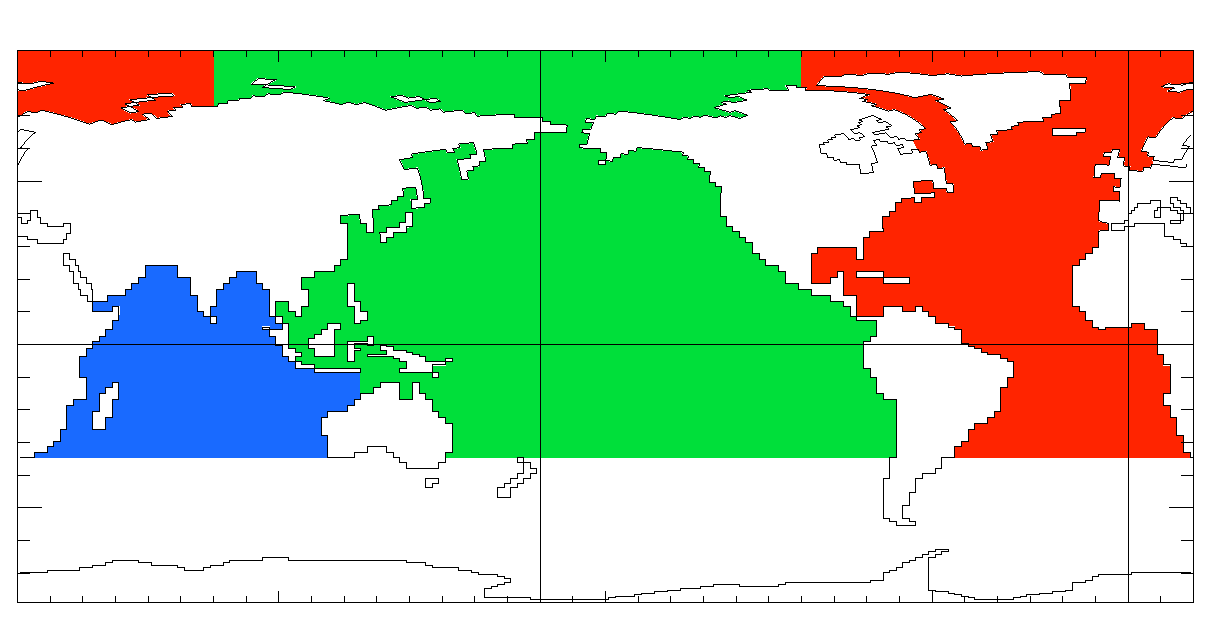
\includegraphics[width=1.0\textwidth]{./TexFiles/Figures/Fig_mask_subasins.pdf}
\caption{	\label{Fig_mask_subasins}
Decomposition of the World Ocean (here ORCA2) into sub-basin used in to compute
the heat and salt transports as well as the meridional stream-function: Atlantic basin (red), 
Pacific basin (green), Indian basin (bleue), Indo-Pacific basin (bleue+green). 
Note that semi-enclosed seas (Red, Med and Baltic seas) as well as Hudson Bay 
are removed from the sub-basins. Note also that the Arctic Ocean has been split 
into Atlantic and Pacific basins along the North fold line.  }
\end{center}   \end{figure}  
%>>>>>>>>>>>>>>>>>>>>>>>>>>>>

In addition, a series of diagnostics has been added in the \mdl{diaar5}. 
They corresponds to outputs that are required for AR5 simulations 
(see Section \ref{DIA_steric} below for one of them). 
Activating those outputs requires to define the \key{diaar5} CPP key.
\\
\\



% ================================================================
% Steric effect in sea surface height
% ================================================================
\section{Diagnosing the Steric effect in sea surface height}
\label{DIA_steric}


Changes in steric sea level are caused when changes in the density of the water 
column imply an expansion or contraction of the column. It is essentially produced 
through surface heating/cooling and to a lesser extent through non-linear effects of 
the equation of state (cabbeling, thermobaricity...).
Non-Boussinesq models contain all ocean effects within the ocean acting 
on the sea level. In particular, they include the steric effect. In contrast, 
Boussinesq models, such as \NEMO, conserve volume, rather than mass, 
and so do not properly represent expansion or contraction. The steric effect is 
therefore not explicitely represented.
This approximation does not represent a serious error with respect to the flow field 
calculated by the model \citep{Greatbatch_JGR94}, but extra attention is required
when investigating sea level, as steric changes are an important 
contribution to local changes in sea level on seasonal and climatic time scales.
This is especially true for investigation into sea level rise due to global warming. 

Fortunately, the steric contribution to the sea level consists of a spatially uniform 
component that can be diagnosed by considering the mass budget of the world 
ocean \citep{Greatbatch_JGR94}. 
In order to better understand how global mean sea level evolves and thus how
the steric sea level can be diagnosed, we compare, in the following, the 
non-Boussinesq and Boussinesq cases.

Let denote 
$\mathcal{M}$ the total mass of liquid seawater ($\mathcal{M}=\int_D \rho dv$), 
$\mathcal{V}$ the total volume of seawater ($\mathcal{V}=\int_D dv$), 
$\mathcal{A}$ the total surface of the ocean ($\mathcal{A}=\int_S ds$), 
$\bar{\rho}$ the global mean seawater (\textit{in situ}) density ($\bar{\rho}= 1/\mathcal{V} \int_D \rho \,dv$), and
$\bar{\eta}$ the global mean sea level ($\bar{\eta}=1/\mathcal{A}\int_S \eta \,ds$).

A non-Boussinesq fluid conserves mass. It satisfies the following relations:
\begin{equation} \label{Eq_MV_nBq} 
\begin{split} 
\mathcal{M} &=  \mathcal{V}  \;\bar{\rho}      	\\
\mathcal{V} &=  \mathcal{A}  \;\bar{\eta}	
\end{split}
\end{equation}
Temporal changes in total mass is obtained from the density conservation equation :
\begin{equation}  \label{Eq_Co_nBq}
\frac{1}{e_3} \partial_t ( e_3\,\rho) + \nabla( \rho \, \textbf{U} ) = \left. \frac{\textit{emp}}{e_3}\right|_\textit{surface}
\end{equation}
where $\rho$ is the \textit{in situ} density, and \textit{emp} the surface mass 
exchanges with the other media of the Earth system (atmosphere, sea-ice, land). 
Its global averaged leads to the total mass change 
\begin{equation}  \label{Eq_Mass_nBq}
\partial_t \mathcal{M} = \mathcal{A} \;\overline{\textit{emp}}
\end{equation}
where $\overline{\textit{emp}}=\int_S \textit{emp}\,ds$ is the net mass flux 
through the ocean surface.
Bringing \eqref{Eq_Mass_nBq} and the time derivative of \eqref{Eq_MV_nBq} 
together leads to the evolution equation of the mean sea level
\begin{equation} \label{Eq_ssh_nBq}
  \partial_t \bar{\eta} =  \frac{\overline{\textit{emp}}}{ \bar{\rho}} 
  					- \frac{\mathcal{V}}{\mathcal{A}}  \;\frac{\partial_t \bar{\rho} }{\bar{\rho}}
\end{equation}
The first term in equation \eqref{Eq_ssh_nBq} alters sea level by adding or 
subtracting mass from the ocean. 
The second term arises from temporal changes in the global mean 
density; $i.e.$ from steric effects. 

In a Boussinesq fluid, $\rho$ is replaced by $\rho_o$ in all the equation except when $\rho$ 
appears multiplied by the gravity ($i.e.$ in the hydrostatic balance of the primitive Equations). 
In particular, the mass conservation equation, \eqref{Eq_Co_nBq}, degenerates into 
the incompressibility equation:
\begin{equation}  \label{Eq_Co_Bq}
\frac{1}{e_3} \partial_t ( e_3 ) + \nabla( \textbf{U} ) =  \left. \frac{\textit{emp}}{\rho_o \,e_3}\right|_ \textit{surface}
\end{equation}
and the global average of this equation now gives the temporal change of the total volume,
\begin{equation}  \label{Eq_V_Bq}
  \partial_t \mathcal{V} =   \mathcal{A} \;\frac{\overline{\textit{emp}}}{\rho_o} 
\end{equation}
Only the volume is conserved, not mass, or, more precisely, the mass which is conserved is the 
Boussinesq mass, $\mathcal{M}_o = \rho_o \mathcal{V}$. The total volume (or equivalently  
the global mean sea level) is altered only by net volume fluxes across the ocean surface,  
not by changes in mean mass of the ocean: the steric effect is missing in a Boussinesq fluid.
 
Nevertheless, following \citep{Greatbatch_JGR94}, the steric effect on the volume can be 
diagnosed by considering the mass budget of the ocean. 
The apparent changes in $\mathcal{M}$, mass of the ocean, which are not induced by surface 
mass flux must be compensated by a spatially uniform change in the mean sea level due to 
expansion/contraction of the ocean \citep{Greatbatch_JGR94}. In others words, the Boussinesq 
mass, $\mathcal{M}_o$, can be related to $\mathcal{M}$, the  total mass of the ocean seen 
by the Boussinesq model, via the steric contribution to the sea level, $\eta_s$, a spatially 
uniform variable, as follows:
\begin{equation}  \label{Eq_M_Bq}
   \mathcal{M}_o  =  \mathcal{M} + \rho_o \,\eta_s \,\mathcal{A} 
\end{equation}
Any change in $\mathcal{M}$ which cannot be explained by the net mass flux through 
the ocean surface is converted into a mean change in sea level. Introducing the total density 
anomaly, $\mathcal{D}= \int_D d_a \,dv$, where $d_a= (\rho -\rho_o ) / \rho_o$  
is the density anomaly used in \NEMO (cf. \S\ref{TRA_eos}) in \eqref{Eq_M_Bq}
leads to a very simple form for the steric height:
\begin{equation}  \label{Eq_steric_Bq}
   \eta_s = - \frac{1}{\mathcal{A}} \mathcal{D} 
\end{equation}

The above formulation of the steric height of a Boussinesq ocean requires four remarks.
First, one can be tempted to define $\rho_o$ as the initial value of $\mathcal{M}/\mathcal{V}$,
$i.e.$ set $\mathcal{D}_{t=0}=0$, so that the initial steric height is zero. We do not
recommend that. Indeed, in this case $\rho_o$ depends on the initial state of the ocean. 
Since $\rho_o$ has a direct effect on the dynamics of the ocean (it appears in the pressure 
gradient term of the momentum equation) it is definitively not a good idea when 
inter-comparing experiments. 
We better recommend to fixe once for all $\rho_o$ to $1035\;Kg\,m^{-3}$. This value is a 
sensible choice for the reference density used in a Boussinesq ocean climate model since, 
with the exception of only a small percentage of the ocean, density in the World Ocean 
varies by no more than 2$\%$ from this value (\cite{Gill1982}, page 47).

Second, we have assumed here that the total ocean surface, $\mathcal{A}$, does not
change when the sea level is changing as it is the case in all global ocean GCMs 
(wetting and drying of grid point is not allowed). 
  
Third, the discretisation of \eqref{Eq_steric_Bq} depends on the type of free surface
which is considered. In the non linear free surface case, $i.e.$ \key{vvl} defined, it is
given by
\begin{equation}  \label{Eq_discrete_steric_Bq}
   \eta_s =  - \frac{ \sum_{i,\,j,\,k} d_a\; e_{1t} e_{2t} e_{3t} }
   					{ \sum_{i,\,j,\,k}         e_{1t} e_{2t} e_{3t} } 
\end{equation}
whereas in the linear free surface, the volume above the \textit{z=0} surface must be explicitly taken 
into account to better approximate the total ocean mass and thus the steric sea level:
\begin{equation}  \label{Eq_discrete_steric_Bq}
   \eta_s =  - \frac{ \sum_{i,\,j,\,k} d_a\; e_{1t}e_{2t}e_{3t} + \sum_{i,\,j} d_a\; e_{1t}e_{2t} \eta }
   						{\sum_{i,\,j,\,k} e_{1t}e_{2t}e_{3t} + \sum_{i,\,j}           e_{1t}e_{2t} \eta } 
\end{equation}

The fourth and last remark concerns the effective sea level and the presence of sea-ice.
In the real ocean, sea ice (and snow above it)  depresses the liquid seawater through 
its mass loading. This depression is a result of the mass of sea ice/snow system acting 
on the liquid ocean. There is, however, no dynamical effect associated with these depressions 
in the liquid ocean sea level, so that there are no associated ocean currents. Hence, the 
dynamically relevant sea level is the effective sea level, $i.e.$ the sea level as if sea ice 
(and snow) were converted to liquid seawater \citep{Campin_al_OM08}. However,
in the current version of \NEMO the sea-ice is levitating above the ocean without 
mass exchanges between ice and ocean. Therefore the model effective sea level
is always given by $\eta + \eta_s$, whether or not there is sea ice present.

In AR5 outputs, the thermosteric sea level is demanded. It is steric sea level due to 
changes in ocean density arising just from changes in temperature. It is given by:
\begin{equation}  \label{Eq_thermosteric_Bq}
   \eta_s = - \frac{1}{\mathcal{A}} \int_D d_a(T,S_o,p_o) \,dv
\end{equation}
where $S_o$ and $p_o$ are the initial salinity and pressure, respectively.

Both steric and thermosteric sea level are computed in \mdl{diaar5} which needs
the \key{diaar5} defined to be called.

% ================================================================












			% Outputs and Diagnostics

% ================================================================
% Chapter observation operator (OBS)
% ================================================================
\chapter{Observation and model comparison (OBS)}
\label{OBS}

Authors: D. Lea, M. Martin, K. Mogensen, A. Vidard, A. Weaver, A. Ryan, ...   % do we keep that ?

\minitoc


\newpage
$\ $\newline    % force a new line

The observation and model comparison code (OBS) reads in observation files (profile
temperature and salinity, sea surface temperature, sea level anomaly, sea ice concentration,
and velocity) and calculates  an interpolated model equivalent value at the observation
location and nearest model timestep. The resulting data are saved in a ``feedback'' file (or
files). The code was originally developed for use with the NEMOVAR data assimilation code, but
can be used for validation or verification of model or  any other data assimilation system.

The OBS code is called from \mdl{nemogcm.F90} for model initialisation and to calculate the model
equivalent values for observations on the 0th timestep. The code is then called again after
each timestep from \mdl{step.F90}. To build with the OBS code active \key{diaobs} must be
set.

For all data types a 2D horizontal  interpolator is needed to interpolate the model fields to
the observation location. For {\em in situ} profiles, a 1D vertical interpolator is needed in
addition to provide model fields at the observation depths. Currently this only works in
z-level model configurations, but is being developed to work with a generalised vertical
coordinate system. Temperature data from moored buoys (TAO, TRITON, PIRATA) in the
ENACT/ENSEMBLES data-base are available as daily averaged quantities. For this type of
observation the observation operator will compare such observations to the model temperature
fields averaged over one day. The relevant observation type may be specified in the namelist
using \np{endailyavtypes}. Otherwise the model value from the nearest timestep to the
observation time is used.

The code is controlled by the namelist \textit{nam\_obs}. See the following sections for more
details on setting up the namelist. 

Section~\ref{OBS_example} introduces a test example of the observation operator code including
where to obtain data and how to setup the namelist. Section~\ref{OBS_details} introduces some
more technical details of the different observation types used and also shows a more complete
namelist. Section~\ref{OBS_theory} introduces some of the theoretical aspects of the observation
operator including interpolation methods and running on multiple processors.
Section~\ref{OBS_ooo} describes the offline observation operator code.
Section~\ref{OBS_obsutils} introduces some utilities to help working with the files
produced by the OBS code.

% ================================================================
% Example
% ================================================================
\section{Running the observation operator code example}
\label{OBS_example}

This section describes an example of running the observation operator code using
profile data which can be freely downloaded. It shows how to adapt an
existing run and build of NEMO to run the observation operator.

\begin{enumerate}
\item Compile NEMO with \key{diaobs} set.

\item Download some ENSEMBLES EN3 data from 
\href{http://www.hadobs.org}{http://www.hadobs.org}. Choose observations which are
valid for the period of your test run because the observation operator compares
the model and observations for a matching date and time. 

\item Add the following to the NEMO namelist to run the observation
operator on this data. Set the \np{enactfiles} namelist variable to the
observation  file name:
\end{enumerate}

%------------------------------------------namobs_example-----------------------------------------------------
\namdisplay{namobs_example}
%-------------------------------------------------------------------------------------------------------------

Options are defined through the  \ngn{namobs} namelist variables.
The options \np{ln\_t3d} and \np{ln\_s3d} switch on the temperature and salinity
profile observation operator code. The \np{ln\_ena} switch turns on the reading
of ENACT/ENSEMBLES type profile data. The filename or array of filenames are
specified using the \np{enactfiles} variable. The model grid points for a
particular  observation latitude and longitude are found using the grid
searching part of the code. This can be expensive, particularly for large
numbers of observations, setting \np{ln\_grid\_search\_lookup} allows the use of
a lookup table which is saved into an ``xypos`` file (or files). This will need
to be generated the first time if it does not exist in the run directory.
However, once produced it will significantly speed up future grid searches.
Setting \np{ln\_grid\_global} means that the code distributes the observations
evenly between processors. Alternatively each processor will work with
observations located within the model subdomain (see section~\ref{OBS_parallel}).

A number of utilities are now provided to plot the feedback files, convert and
recombine the files. These are explained in more detail in section~\ref{OBS_obsutils}.

\section{Technical details}
\label{OBS_details}

Here we show a more complete example namelist  \ngn{namobs} and also show the NetCDF headers
of the observation
files that may be used with the observation operator

%------------------------------------------namobs--------------------------------------------------------
\namdisplay{namobs}
%-------------------------------------------------------------------------------------------------------------

This name list uses the "feedback" type observation file input format for
profile, sea level anomaly and sea surface temperature data. All the
observation files must be in NetCDF format. Some example headers (produced using
\mbox{\textit{ncdump~-h}}) for profile
data, sea level anomaly and sea surface temperature are in the following
subsections.

\subsection{Profile feedback type observation file header}

\begin{alltt}
\tiny
\begin{verbatim}
netcdf profiles_01 {
dimensions:
     N_OBS = 603 ;
     N_LEVELS = 150 ;
     N_VARS = 2 ;
     N_QCF = 2 ;
     N_ENTRIES = 1 ;
     N_EXTRA = 1 ;
     STRINGNAM = 8 ;
     STRINGGRID = 1 ;
     STRINGWMO = 8 ;
     STRINGTYP = 4 ;
     STRINGJULD = 14 ;
variables:
     char VARIABLES(N_VARS, STRINGNAM) ;
          VARIABLES:long_name = "List of variables in feedback files" ;
     char ENTRIES(N_ENTRIES, STRINGNAM) ;
          ENTRIES:long_name = "List of additional entries for each variable in feedback files" ;
     char EXTRA(N_EXTRA, STRINGNAM) ;
          EXTRA:long_name = "List of extra variables" ;
     char STATION_IDENTIFIER(N_OBS, STRINGWMO) ;
          STATION_IDENTIFIER:long_name = "Station identifier" ;
     char STATION_TYPE(N_OBS, STRINGTYP) ;
          STATION_TYPE:long_name = "Code instrument type" ;
     double LONGITUDE(N_OBS) ;
          LONGITUDE:long_name = "Longitude" ;
          LONGITUDE:units = "degrees_east" ;
          LONGITUDE:_Fillvalue = 99999.f ;
     double LATITUDE(N_OBS) ;
          LATITUDE:long_name = "Latitude" ;
          LATITUDE:units = "degrees_north" ;
          LATITUDE:_Fillvalue = 99999.f ;
     double DEPTH(N_OBS, N_LEVELS) ;
          DEPTH:long_name = "Depth" ;
          DEPTH:units = "metre" ;
          DEPTH:_Fillvalue = 99999.f ;
     int DEPTH_QC(N_OBS, N_LEVELS) ;
          DEPTH_QC:long_name = "Quality on depth" ;
          DEPTH_QC:Conventions = "q where q =[0,9]" ;
          DEPTH_QC:_Fillvalue = 0 ;
     int DEPTH_QC_FLAGS(N_OBS, N_LEVELS, N_QCF) ;
          DEPTH_QC_FLAGS:long_name = "Quality flags on depth" ;
          DEPTH_QC_FLAGS:Conventions = "NEMOVAR flag conventions" ;
     double JULD(N_OBS) ;
          JULD:long_name = "Julian day" ;
          JULD:units = "days since JULD_REFERENCE" ;
          JULD:Conventions = "relative julian days with decimal part (as parts of day)" ;
          JULD:_Fillvalue = 99999.f ;
     char JULD_REFERENCE(STRINGJULD) ;
          JULD_REFERENCE:long_name = "Date of reference for julian days" ;
          JULD_REFERENCE:Conventions = "YYYYMMDDHHMMSS" ;
     int OBSERVATION_QC(N_OBS) ;
          OBSERVATION_QC:long_name = "Quality on observation" ;
          OBSERVATION_QC:Conventions = "q where q =[0,9]" ;
          OBSERVATION_QC:_Fillvalue = 0 ;
     int OBSERVATION_QC_FLAGS(N_OBS, N_QCF) ;
          OBSERVATION_QC_FLAGS:long_name = "Quality flags on observation" ;
          OBSERVATION_QC_FLAGS:Conventions = "NEMOVAR flag conventions" ;
          OBSERVATION_QC_FLAGS:_Fillvalue = 0 ;
     int POSITION_QC(N_OBS) ;
          POSITION_QC:long_name = "Quality on position (latitude and longitude)" ;
          POSITION_QC:Conventions = "q where q =[0,9]" ;
          POSITION_QC:_Fillvalue = 0 ;
     int POSITION_QC_FLAGS(N_OBS, N_QCF) ;
          POSITION_QC_FLAGS:long_name = "Quality flags on position" ;
          POSITION_QC_FLAGS:Conventions = "NEMOVAR flag conventions" ;
          POSITION_QC_FLAGS:_Fillvalue = 0 ;
     int JULD_QC(N_OBS) ;
          JULD_QC:long_name = "Quality on date and time" ;
          JULD_QC:Conventions = "q where q =[0,9]" ;
          JULD_QC:_Fillvalue = 0 ;
     int JULD_QC_FLAGS(N_OBS, N_QCF) ;
          JULD_QC_FLAGS:long_name = "Quality flags on date and time" ;
          JULD_QC_FLAGS:Conventions = "NEMOVAR flag conventions" ;
          JULD_QC_FLAGS:_Fillvalue = 0 ;
     int ORIGINAL_FILE_INDEX(N_OBS) ;
          ORIGINAL_FILE_INDEX:long_name = "Index in original data file" ;
          ORIGINAL_FILE_INDEX:_Fillvalue = -99999 ;
     float POTM_OBS(N_OBS, N_LEVELS) ;
          POTM_OBS:long_name = "Potential temperature" ;
          POTM_OBS:units = "Degrees Celsius" ;
          POTM_OBS:_Fillvalue = 99999.f ;
     float POTM_Hx(N_OBS, N_LEVELS) ;
          POTM_Hx:long_name = "Model interpolated potential temperature" ;
          POTM_Hx:units = "Degrees Celsius" ;
          POTM_Hx:_Fillvalue = 99999.f ;
     int POTM_QC(N_OBS) ;
          POTM_QC:long_name = "Quality on potential temperature" ;
          POTM_QC:Conventions = "q where q =[0,9]" ;
          POTM_QC:_Fillvalue = 0 ;
     int POTM_QC_FLAGS(N_OBS, N_QCF) ;
          POTM_QC_FLAGS:long_name = "Quality flags on potential temperature" ;
          POTM_QC_FLAGS:Conventions = "NEMOVAR flag conventions" ;
          POTM_QC_FLAGS:_Fillvalue = 0 ;
     int POTM_LEVEL_QC(N_OBS, N_LEVELS) ;
          POTM_LEVEL_QC:long_name = "Quality for each level on potential temperature" ;
          POTM_LEVEL_QC:Conventions = "q where q =[0,9]" ;
          POTM_LEVEL_QC:_Fillvalue = 0 ;
     int POTM_LEVEL_QC_FLAGS(N_OBS, N_LEVELS, N_QCF) ;
          POTM_LEVEL_QC_FLAGS:long_name = "Quality flags for each level on potential temperature" ;
          POTM_LEVEL_QC_FLAGS:Conventions = "NEMOVAR flag conventions" ;
          POTM_LEVEL_QC_FLAGS:_Fillvalue = 0 ;
     int POTM_IOBSI(N_OBS) ;
          POTM_IOBSI:long_name = "ORCA grid search I coordinate" ;
     int POTM_IOBSJ(N_OBS) ;
          POTM_IOBSJ:long_name = "ORCA grid search J coordinate" ;
     int POTM_IOBSK(N_OBS, N_LEVELS) ;
          POTM_IOBSK:long_name = "ORCA grid search K coordinate" ;
     char POTM_GRID(STRINGGRID) ;
          POTM_GRID:long_name = "ORCA grid search grid (T,U,V)" ;
     float PSAL_OBS(N_OBS, N_LEVELS) ;
          PSAL_OBS:long_name = "Practical salinity" ;
          PSAL_OBS:units = "PSU" ;
          PSAL_OBS:_Fillvalue = 99999.f ;
     float PSAL_Hx(N_OBS, N_LEVELS) ;
          PSAL_Hx:long_name = "Model interpolated practical salinity" ;
          PSAL_Hx:units = "PSU" ;
          PSAL_Hx:_Fillvalue = 99999.f ;
     int PSAL_QC(N_OBS) ;
          PSAL_QC:long_name = "Quality on practical salinity" ;
          PSAL_QC:Conventions = "q where q =[0,9]" ;
          PSAL_QC:_Fillvalue = 0 ;
     int PSAL_QC_FLAGS(N_OBS, N_QCF) ;
          PSAL_QC_FLAGS:long_name = "Quality flags on practical salinity" ;
          PSAL_QC_FLAGS:Conventions = "NEMOVAR flag conventions" ;
          PSAL_QC_FLAGS:_Fillvalue = 0 ;
     int PSAL_LEVEL_QC(N_OBS, N_LEVELS) ;
          PSAL_LEVEL_QC:long_name = "Quality for each level on practical salinity" ;
          PSAL_LEVEL_QC:Conventions = "q where q =[0,9]" ;
          PSAL_LEVEL_QC:_Fillvalue = 0 ;
     int PSAL_LEVEL_QC_FLAGS(N_OBS, N_LEVELS, N_QCF) ;
          PSAL_LEVEL_QC_FLAGS:long_name = "Quality flags for each level on practical salinity" ;
          PSAL_LEVEL_QC_FLAGS:Conventions = "NEMOVAR flag conventions" ;
          PSAL_LEVEL_QC_FLAGS:_Fillvalue = 0 ;
     int PSAL_IOBSI(N_OBS) ;
          PSAL_IOBSI:long_name = "ORCA grid search I coordinate" ;
     int PSAL_IOBSJ(N_OBS) ;
          PSAL_IOBSJ:long_name = "ORCA grid search J coordinate" ;
     int PSAL_IOBSK(N_OBS, N_LEVELS) ;
          PSAL_IOBSK:long_name = "ORCA grid search K coordinate" ;
     char PSAL_GRID(STRINGGRID) ;
          PSAL_GRID:long_name = "ORCA grid search grid (T,U,V)" ;
     float TEMP(N_OBS, N_LEVELS) ;
          TEMP:long_name = "Insitu temperature" ;
          TEMP:units = "Degrees Celsius" ;
          TEMP:_Fillvalue = 99999.f ;

// global attributes:
          :title = "NEMO observation operator output" ;
          :Convention = "NEMO unified observation operator output" ;
}
\end{verbatim}
\end{alltt}

\subsection{Sea level anomaly feedback type observation file header}

\begin{alltt}
\tiny
\begin{verbatim}
netcdf sla_01 {
dimensions:
     N_OBS = 41301 ;
     N_LEVELS = 1 ;
     N_VARS = 1 ;
     N_QCF = 2 ;
     N_ENTRIES = 1 ;
     N_EXTRA = 1 ;
     STRINGNAM = 8 ;
     STRINGGRID = 1 ;
     STRINGWMO = 8 ;
     STRINGTYP = 4 ;
     STRINGJULD = 14 ;
variables:
     char VARIABLES(N_VARS, STRINGNAM) ;
          VARIABLES:long_name = "List of variables in feedback files" ;
     char ENTRIES(N_ENTRIES, STRINGNAM) ;
          ENTRIES:long_name = "List of additional entries for each variable in feedback files" ;
     char EXTRA(N_EXTRA, STRINGNAM) ;
          EXTRA:long_name = "List of extra variables" ;
     char STATION_IDENTIFIER(N_OBS, STRINGWMO) ;
          STATION_IDENTIFIER:long_name = "Station identifier" ;
     char STATION_TYPE(N_OBS, STRINGTYP) ;
          STATION_TYPE:long_name = "Code instrument type" ;
     double LONGITUDE(N_OBS) ;
          LONGITUDE:long_name = "Longitude" ;
          LONGITUDE:units = "degrees_east" ;
          LONGITUDE:_Fillvalue = 99999.f ;
     double LATITUDE(N_OBS) ;
          LATITUDE:long_name = "Latitude" ;
          LATITUDE:units = "degrees_north" ;
          LATITUDE:_Fillvalue = 99999.f ;
     double DEPTH(N_OBS, N_LEVELS) ;
          DEPTH:long_name = "Depth" ;
          DEPTH:units = "metre" ;
          DEPTH:_Fillvalue = 99999.f ;
     int DEPTH_QC(N_OBS, N_LEVELS) ;
          DEPTH_QC:long_name = "Quality on depth" ;
          DEPTH_QC:Conventions = "q where q =[0,9]" ;
          DEPTH_QC:_Fillvalue = 0 ;
     int DEPTH_QC_FLAGS(N_OBS, N_LEVELS, N_QCF) ;
          DEPTH_QC_FLAGS:long_name = "Quality flags on depth" ;
          DEPTH_QC_FLAGS:Conventions = "NEMOVAR flag conventions" ;
     double JULD(N_OBS) ;
          JULD:long_name = "Julian day" ;
          JULD:units = "days since JULD_REFERENCE" ;
          JULD:Conventions = "relative julian days with decimal part (as parts of day)" ;
          JULD:_Fillvalue = 99999.f ;
     char JULD_REFERENCE(STRINGJULD) ;
          JULD_REFERENCE:long_name = "Date of reference for julian days" ;
          JULD_REFERENCE:Conventions = "YYYYMMDDHHMMSS" ;
     int OBSERVATION_QC(N_OBS) ;
          OBSERVATION_QC:long_name = "Quality on observation" ;
          OBSERVATION_QC:Conventions = "q where q =[0,9]" ;
          OBSERVATION_QC:_Fillvalue = 0 ;
     int OBSERVATION_QC_FLAGS(N_OBS, N_QCF) ;
          OBSERVATION_QC_FLAGS:long_name = "Quality flags on observation" ;
          OBSERVATION_QC_FLAGS:Conventions = "NEMOVAR flag conventions" ;
          OBSERVATION_QC_FLAGS:_Fillvalue = 0 ;
     int POSITION_QC(N_OBS) ;
          POSITION_QC:long_name = "Quality on position (latitude and longitude)" ;
          POSITION_QC:Conventions = "q where q =[0,9]" ;
          POSITION_QC:_Fillvalue = 0 ;
     int POSITION_QC_FLAGS(N_OBS, N_QCF) ;
          POSITION_QC_FLAGS:long_name = "Quality flags on position" ;
          POSITION_QC_FLAGS:Conventions = "NEMOVAR flag conventions" ;
          POSITION_QC_FLAGS:_Fillvalue = 0 ;
     int JULD_QC(N_OBS) ;
          JULD_QC:long_name = "Quality on date and time" ;
          JULD_QC:Conventions = "q where q =[0,9]" ;
          JULD_QC:_Fillvalue = 0 ;
     int JULD_QC_FLAGS(N_OBS, N_QCF) ;
          JULD_QC_FLAGS:long_name = "Quality flags on date and time" ;
          JULD_QC_FLAGS:Conventions = "NEMOVAR flag conventions" ;
          JULD_QC_FLAGS:_Fillvalue = 0 ;
     int ORIGINAL_FILE_INDEX(N_OBS) ;
          ORIGINAL_FILE_INDEX:long_name = "Index in original data file" ;
          ORIGINAL_FILE_INDEX:_Fillvalue = -99999 ;
     float SLA_OBS(N_OBS, N_LEVELS) ;
          SLA_OBS:long_name = "Sea level anomaly" ;
          SLA_OBS:units = "metre" ;
          SLA_OBS:_Fillvalue = 99999.f ;
     float SLA_Hx(N_OBS, N_LEVELS) ;
          SLA_Hx:long_name = "Model interpolated sea level anomaly" ;
          SLA_Hx:units = "metre" ;
          SLA_Hx:_Fillvalue = 99999.f ;
     int SLA_QC(N_OBS) ;
          SLA_QC:long_name = "Quality on sea level anomaly" ;
          SLA_QC:Conventions = "q where q =[0,9]" ;
          SLA_QC:_Fillvalue = 0 ;
     int SLA_QC_FLAGS(N_OBS, N_QCF) ;
          SLA_QC_FLAGS:long_name = "Quality flags on sea level anomaly" ;
          SLA_QC_FLAGS:Conventions = "NEMOVAR flag conventions" ;
          SLA_QC_FLAGS:_Fillvalue = 0 ;
     int SLA_LEVEL_QC(N_OBS, N_LEVELS) ;
          SLA_LEVEL_QC:long_name = "Quality for each level on sea level anomaly" ;
          SLA_LEVEL_QC:Conventions = "q where q =[0,9]" ;
          SLA_LEVEL_QC:_Fillvalue = 0 ;
     int SLA_LEVEL_QC_FLAGS(N_OBS, N_LEVELS, N_QCF) ;
          SLA_LEVEL_QC_FLAGS:long_name = "Quality flags for each level on sea level anomaly" ;
          SLA_LEVEL_QC_FLAGS:Conventions = "NEMOVAR flag conventions" ;
          SLA_LEVEL_QC_FLAGS:_Fillvalue = 0 ;
     int SLA_IOBSI(N_OBS) ;
          SLA_IOBSI:long_name = "ORCA grid search I coordinate" ;
     int SLA_IOBSJ(N_OBS) ;
          SLA_IOBSJ:long_name = "ORCA grid search J coordinate" ;
     int SLA_IOBSK(N_OBS, N_LEVELS) ;
          SLA_IOBSK:long_name = "ORCA grid search K coordinate" ;
     char SLA_GRID(STRINGGRID) ;
          SLA_GRID:long_name = "ORCA grid search grid (T,U,V)" ;
     float MDT(N_OBS, N_LEVELS) ;
          MDT:long_name = "Mean Dynamic Topography" ;
          MDT:units = "metre" ;
          MDT:_Fillvalue = 99999.f ;

// global attributes:
          :title = "NEMO observation operator output" ;
          :Convention = "NEMO unified observation operator output" ;
}
\end{verbatim}
\end{alltt}

The mean dynamic
topography (MDT) must be provided in a separate file defined on the model grid
 called {\it slaReferenceLevel.nc}. The MDT is required in
order to produce the model equivalent sea level anomaly from the model sea
surface height. Below is an example header for this file (on the ORCA025 grid).

\begin{alltt}
\tiny
\begin{verbatim}
dimensions:
        x = 1442 ;
        y = 1021 ;
variables:
        float nav_lon(y, x) ;
                nav_lon:units = "degrees_east" ;
        float nav_lat(y, x) ;
                nav_lat:units = "degrees_north" ;
        float sossheig(y, x) ;
                sossheig:_FillValue = -1.e+30f ;
                sossheig:coordinates = "nav_lon nav_lat" ;
                sossheig:long_name = "Mean Dynamic Topography" ;
                sossheig:units = "metres" ;
                sossheig:grid = "orca025T" ;
\end{verbatim}
\end{alltt}

\subsection{Sea surface temperature feedback type observation file header}

\begin{alltt}
\tiny
\begin{verbatim}
netcdf sst_01 {
dimensions:
     N_OBS = 33099 ;
     N_LEVELS = 1 ;
     N_VARS = 1 ;
     N_QCF = 2 ;
     N_ENTRIES = 1 ;
     STRINGNAM = 8 ;
     STRINGGRID = 1 ;
     STRINGWMO = 8 ;
     STRINGTYP = 4 ;
     STRINGJULD = 14 ;
variables:
     char VARIABLES(N_VARS, STRINGNAM) ;
          VARIABLES:long_name = "List of variables in feedback files" ;
     char ENTRIES(N_ENTRIES, STRINGNAM) ;
          ENTRIES:long_name = "List of additional entries for each variable in feedback files" ;
     char STATION_IDENTIFIER(N_OBS, STRINGWMO) ;
          STATION_IDENTIFIER:long_name = "Station identifier" ;
     char STATION_TYPE(N_OBS, STRINGTYP) ;
          STATION_TYPE:long_name = "Code instrument type" ;
     double LONGITUDE(N_OBS) ;
          LONGITUDE:long_name = "Longitude" ;
          LONGITUDE:units = "degrees_east" ;
          LONGITUDE:_Fillvalue = 99999.f ;
     double LATITUDE(N_OBS) ;
          LATITUDE:long_name = "Latitude" ;
          LATITUDE:units = "degrees_north" ;
          LATITUDE:_Fillvalue = 99999.f ;
     double DEPTH(N_OBS, N_LEVELS) ;
          DEPTH:long_name = "Depth" ;
          DEPTH:units = "metre" ;
          DEPTH:_Fillvalue = 99999.f ;
     int DEPTH_QC(N_OBS, N_LEVELS) ;
          DEPTH_QC:long_name = "Quality on depth" ;
          DEPTH_QC:Conventions = "q where q =[0,9]" ;
          DEPTH_QC:_Fillvalue = 0 ;
     int DEPTH_QC_FLAGS(N_OBS, N_LEVELS, N_QCF) ;
          DEPTH_QC_FLAGS:long_name = "Quality flags on depth" ;
          DEPTH_QC_FLAGS:Conventions = "NEMOVAR flag conventions" ;
     double JULD(N_OBS) ;
          JULD:long_name = "Julian day" ;
          JULD:units = "days since JULD_REFERENCE" ;
          JULD:Conventions = "relative julian days with decimal part (as parts of day)" ;
          JULD:_Fillvalue = 99999.f ;
     char JULD_REFERENCE(STRINGJULD) ;
          JULD_REFERENCE:long_name = "Date of reference for julian days" ;
          JULD_REFERENCE:Conventions = "YYYYMMDDHHMMSS" ;
     int OBSERVATION_QC(N_OBS) ;
          OBSERVATION_QC:long_name = "Quality on observation" ;
          OBSERVATION_QC:Conventions = "q where q =[0,9]" ;
          OBSERVATION_QC:_Fillvalue = 0 ;
     int OBSERVATION_QC_FLAGS(N_OBS, N_QCF) ;
          OBSERVATION_QC_FLAGS:long_name = "Quality flags on observation" ;
          OBSERVATION_QC_FLAGS:Conventions = "NEMOVAR flag conventions" ;
          OBSERVATION_QC_FLAGS:_Fillvalue = 0 ;
     int POSITION_QC(N_OBS) ;
          POSITION_QC:long_name = "Quality on position (latitude and longitude)" ;
          POSITION_QC:Conventions = "q where q =[0,9]" ;
          POSITION_QC:_Fillvalue = 0 ;
     int POSITION_QC_FLAGS(N_OBS, N_QCF) ;
          POSITION_QC_FLAGS:long_name = "Quality flags on position" ;
          POSITION_QC_FLAGS:Conventions = "NEMOVAR flag conventions" ;
          POSITION_QC_FLAGS:_Fillvalue = 0 ;
     int JULD_QC(N_OBS) ;
          JULD_QC:long_name = "Quality on date and time" ;
          JULD_QC:Conventions = "q where q =[0,9]" ;
          JULD_QC:_Fillvalue = 0 ;
     int JULD_QC_FLAGS(N_OBS, N_QCF) ;
          JULD_QC_FLAGS:long_name = "Quality flags on date and time" ;
          JULD_QC_FLAGS:Conventions = "NEMOVAR flag conventions" ;
          JULD_QC_FLAGS:_Fillvalue = 0 ;
     int ORIGINAL_FILE_INDEX(N_OBS) ;
          ORIGINAL_FILE_INDEX:long_name = "Index in original data file" ;
          ORIGINAL_FILE_INDEX:_Fillvalue = -99999 ;
     float SST_OBS(N_OBS, N_LEVELS) ;
          SST_OBS:long_name = "Sea surface temperature" ;
          SST_OBS:units = "Degree centigrade" ;
          SST_OBS:_Fillvalue = 99999.f ;
     float SST_Hx(N_OBS, N_LEVELS) ;
          SST_Hx:long_name = "Model interpolated sea surface temperature" ;
          SST_Hx:units = "Degree centigrade" ;
          SST_Hx:_Fillvalue = 99999.f ;
     int SST_QC(N_OBS) ;
          SST_QC:long_name = "Quality on sea surface temperature" ;
          SST_QC:Conventions = "q where q =[0,9]" ;
          SST_QC:_Fillvalue = 0 ;
     int SST_QC_FLAGS(N_OBS, N_QCF) ;
          SST_QC_FLAGS:long_name = "Quality flags on sea surface temperature" ;
          SST_QC_FLAGS:Conventions = "NEMOVAR flag conventions" ;
          SST_QC_FLAGS:_Fillvalue = 0 ;
     int SST_LEVEL_QC(N_OBS, N_LEVELS) ;
          SST_LEVEL_QC:long_name = "Quality for each level on sea surface temperature" ;
          SST_LEVEL_QC:Conventions = "q where q =[0,9]" ;
          SST_LEVEL_QC:_Fillvalue = 0 ;
     int SST_LEVEL_QC_FLAGS(N_OBS, N_LEVELS, N_QCF) ;
          SST_LEVEL_QC_FLAGS:long_name = "Quality flags for each level on sea surface temperature" ;
          SST_LEVEL_QC_FLAGS:Conventions = "NEMOVAR flag conventions" ;
          SST_LEVEL_QC_FLAGS:_Fillvalue = 0 ;
     int SST_IOBSI(N_OBS) ;
          SST_IOBSI:long_name = "ORCA grid search I coordinate" ;
     int SST_IOBSJ(N_OBS) ;
          SST_IOBSJ:long_name = "ORCA grid search J coordinate" ;
     int SST_IOBSK(N_OBS, N_LEVELS) ;
          SST_IOBSK:long_name = "ORCA grid search K coordinate" ;
     char SST_GRID(STRINGGRID) ;
          SST_GRID:long_name = "ORCA grid search grid (T,U,V)" ;

// global attributes:
          :title = "NEMO observation operator output" ;
          :Convention = "NEMO unified observation operator output" ;
}
\end{verbatim}
\end{alltt}

\section{Theoretical details}
\label{OBS_theory}

\subsection{Horizontal interpolation methods}

Consider an observation point ${\rm P}$ with 
with longitude and latitude $({\lambda_{}}_{\rm P}, \phi_{\rm P})$ and the 
four nearest neighbouring model grid points ${\rm A}$, ${\rm B}$, ${\rm C}$ 
and ${\rm D}$ with longitude and latitude ($\lambda_{\rm A}$, $\phi_{\rm A}$),
($\lambda_{\rm B}$, $\phi_{\rm B}$) etc.
All horizontal interpolation methods implemented in NEMO
estimate the value of a model variable $x$ at point $P$ as
a weighted linear combination of the values of the model 
variables at the grid points ${\rm A}$, ${\rm B}$ etc.:
\begin{eqnarray}
{x_{}}_{\rm P} & \hspace{-2mm} = \hspace{-2mm} & 
\frac{1}{w} \left( {w_{}}_{\rm A} {x_{}}_{\rm A} + 
                   {w_{}}_{\rm B} {x_{}}_{\rm B} + 
                   {w_{}}_{\rm C} {x_{}}_{\rm C} + 
                   {w_{}}_{\rm D} {x_{}}_{\rm D} \right)
\end{eqnarray}
where ${w_{}}_{\rm A}$, ${w_{}}_{\rm B}$ etc. are the respective weights for the 
model field at points ${\rm A}$, ${\rm B}$ etc., and 
$w = {w_{}}_{\rm A} + {w_{}}_{\rm B} + {w_{}}_{\rm C} + {w_{}}_{\rm D}$.

Four different possibilities are available for computing the weights.

\begin{enumerate}

\item[1.] {\bf Great-Circle distance-weighted interpolation.} The weights
  are computed as a function of the great-circle distance $s(P, \cdot)$ 
  between $P$ and the model grid points $A$, $B$ etc. For example, 
  the weight given to the field ${x_{}}_{\rm A}$ is specified as the 
  product of the distances from ${\rm P}$ to the other points:
  \begin{eqnarray}
  {w_{}}_{\rm A} = s({\rm P}, {\rm B}) \, s({\rm P}, {\rm C}) \, s({\rm P}, {\rm D})
  \nonumber
  \end{eqnarray}
  where 
  \begin{eqnarray}
   s\left ({\rm P}, {\rm M} \right ) 
     & \hspace{-2mm} = \hspace{-2mm} & 
      \cos^{-1} \! \left\{ 
               \sin {\phi_{}}_{\rm P} \sin {\phi_{}}_{\rm M}
             + \cos {\phi_{}}_{\rm P} \cos {\phi_{}}_{\rm M} 
               \cos ({\lambda_{}}_{\rm M} - {\lambda_{}}_{\rm P}) 
                   \right\}
   \end{eqnarray}
   and $M$ corresponds to $B$, $C$ or $D$.
   A more stable form of the great-circle distance formula for
   small distances ($x$ near 1) involves the arcsine function
   ($e.g.$ see p.~101 of \citet{Daley_Barker_Bk01}:
   \begin{eqnarray}
   s\left( {\rm P}, {\rm M} \right) 
     & \hspace{-2mm} = \hspace{-2mm} & 
      \sin^{-1} \! \left\{ \sqrt{ 1 - x^2 } \right\}
   \nonumber
   \end{eqnarray}
   where
   \begin{eqnarray}
    x & \hspace{-2mm} = \hspace{-2mm} & 
      {a_{}}_{\rm M} {a_{}}_{\rm P} + {b_{}}_{\rm M} {b_{}}_{\rm P} + {c_{}}_{\rm M} {c_{}}_{\rm P}
   \nonumber
   \end{eqnarray}
   and 
   \begin{eqnarray}
      {a_{}}_{\rm M} & \hspace{-2mm} = \hspace{-2mm} & \sin {\phi_{}}_{\rm M}, 
      \nonumber \\
      {a_{}}_{\rm P} & \hspace{-2mm} = \hspace{-2mm} & \sin {\phi_{}}_{\rm P}, 
      \nonumber \\
      {b_{}}_{\rm M} & \hspace{-2mm} = \hspace{-2mm} & \cos {\phi_{}}_{\rm M} \cos {\phi_{}}_{\rm M}, 
      \nonumber \\
      {b_{}}_{\rm P} & \hspace{-2mm} = \hspace{-2mm} & \cos {\phi_{}}_{\rm P} \cos {\phi_{}}_{\rm P}, 
      \nonumber \\
      {c_{}}_{\rm M} & \hspace{-2mm} = \hspace{-2mm} & \cos {\phi_{}}_{\rm M} \sin {\phi_{}}_{\rm M}, 
      \nonumber \\
      {c_{}}_{\rm P} & \hspace{-2mm} = \hspace{-2mm} & \cos {\phi_{}}_{\rm P} \sin {\phi_{}}_{\rm P}.
      \nonumber
   \nonumber
  \end{eqnarray}

\item[2.] {\bf Great-Circle distance-weighted interpolation with small angle
  approximation.} Similar to the previous interpolation but with the
  distance $s$ computed as
  \begin{eqnarray}
    s\left( {\rm P}, {\rm M} \right) 
     & \hspace{-2mm} = \hspace{-2mm} & 
      \sqrt{ \left( {\phi_{}}_{\rm M} - {\phi_{}}_{\rm P} \right)^{2} 
      + \left( {\lambda_{}}_{\rm M} - {\lambda_{}}_{\rm P} \right)^{2}
        \cos^{2} {\phi_{}}_{\rm M} }
  \end{eqnarray}
  where $M$ corresponds to $A$, $B$, $C$ or $D$.

\item[3.] {\bf Bilinear interpolation for a regular spaced grid.} The
  interpolation is split into two 1D interpolations in the longitude
  and latitude directions, respectively.

\item[4.] {\bf Bilinear remapping interpolation for a general grid.} An
  iterative scheme that involves first mapping a quadrilateral cell
  into a cell with coordinates (0,0), (1,0), (0,1) and (1,1). This
  method is based on the SCRIP interpolation package \citep{Jones_1998}.
  
\end{enumerate}

\subsection{Grid search}

For many grids used by the NEMO model, such as the ORCA family, 
the horizontal grid coordinates $i$ and $j$ are not simple functions 
of latitude and longitude. Therefore, it is not always straightforward 
to determine the grid points surrounding any given observational position.
Before the interpolation can be performed, a search 
algorithm is then required to determine the corner points of 
the quadrilateral cell in which the observation is located.
This is the most difficult and time consuming part of the 
2D interpolation procedure. 
A robust test for determining if an observation falls
within a given quadrilateral cell is as follows. Let 
${\rm P}({\lambda_{}}_{\rm P} ,{\phi_{}}_{\rm P} )$ denote the observation point,
and let ${\rm A}({\lambda_{}}_{\rm A} ,{\phi_{}}_{\rm A} )$,
${\rm B}({\lambda_{}}_{\rm B} ,{\phi_{}}_{\rm B} )$,
${\rm C}({\lambda_{}}_{\rm C} ,{\phi_{}}_{\rm C} )$ 
and 
${\rm D}({\lambda_{}}_{\rm D} ,{\phi_{}}_{\rm D} )$ denote
the bottom left, bottom right, top left and top right
corner points of the cell, respectively. 
To determine if P is inside 
the cell, we verify that the cross-products 
\begin{eqnarray}
\begin{array}{lllll}
{{\bf r}_{}}_{\rm PA} \times {{\bf r}_{}}_{\rm PC}
& = & [({\lambda_{}}_{\rm A}\; -\; {\lambda_{}}_{\rm P} )
      ({\phi_{}}_{\rm C}   \; -\; {\phi_{}}_{\rm P} )
    - ({\lambda_{}}_{\rm C}\; -\; {\lambda_{}}_{\rm P} )
      ({\phi_{}}_{\rm A}   \; -\; {\phi_{}}_{\rm P} )] \; \widehat{\bf k} \\
{{\bf r}_{}}_{\rm PB} \times {{\bf r}_{}}_{\rm PA}
& = & [({\lambda_{}}_{\rm B}\; -\; {\lambda_{}}_{\rm P} )
      ({\phi_{}}_{\rm A}   \; -\; {\phi_{}}_{\rm P} )
    - ({\lambda_{}}_{\rm A}\; -\; {\lambda_{}}_{\rm P} )
      ({\phi_{}}_{\rm B}   \; -\; {\phi_{}}_{\rm P} )] \; \widehat{\bf k} \\
{{\bf r}_{}}_{\rm PC} \times {{\bf r}_{}}_{\rm PD}
& = & [({\lambda_{}}_{\rm C}\; -\; {\lambda_{}}_{\rm P} )
      ({\phi_{}}_{\rm D}   \; -\; {\phi_{}}_{\rm P} )
    - ({\lambda_{}}_{\rm D}\; -\; {\lambda_{}}_{\rm P} )
      ({\phi_{}}_{\rm C}   \; -\; {\phi_{}}_{\rm P} )] \; \widehat{\bf k} \\
{{\bf r}_{}}_{\rm PD} \times {{\bf r}_{}}_{\rm PB}
& = & [({\lambda_{}}_{\rm D}\; -\; {\lambda_{}}_{\rm P} )
      ({\phi_{}}_{\rm B}   \; -\; {\phi_{}}_{\rm P} )
    - ({\lambda_{}}_{\rm B}\; -\; {\lambda_{}}_{\rm P} )
      ({\phi_{}}_{\rm D}  \;  - \; {\phi_{}}_{\rm P} )] \; \widehat{\bf k} \\
\end{array}
\label{eq:cross}
\end{eqnarray}
point in the opposite direction to the unit normal 
$\widehat{\bf k}$ (i.e., that the coefficients of 
$\widehat{\bf k}$ are negative),
where ${{\bf r}_{}}_{\rm PA}$, ${{\bf r}_{}}_{\rm PB}$, 
etc. correspond to the vectors between points P and A, 
P and B, etc.. The method used is
similar to the method used in
the SCRIP interpolation package \citep{Jones_1998}.

In order to speed up the grid search, there is the possibility to construct 
a lookup table for a user specified resolution. This lookup
table contains the lower and upper bounds on the $i$ and $j$ indices
to be searched for on a regular grid. For each observation position,
the closest point on the regular grid of this position is computed and
the $i$ and $j$ ranges of this point searched to determine the precise
four points surrounding the observation. 

\subsection{Parallel aspects of horizontal interpolation}
\label{OBS_parallel}

For horizontal interpolation, there is the basic problem that the
observations are unevenly distributed on the globe. In numerical
models, it is common to divide the model grid into subgrids (or
domains) where each subgrid is executed on a single processing element
with explicit message passing for exchange of information along the
domain boundaries when running on a massively parallel processor (MPP)
system. This approach is used by \NEMO.

For observations there is no natural distribution since the
observations are not equally distributed on the globe. 
Two options have been made available: 1) geographical distribution;
and 2) round-robin.

\subsubsection{Geographical distribution of observations among processors}

%>>>>>>>>>>>>>>>>>>>>>>>>>>>>
\begin{figure}      \begin{center}
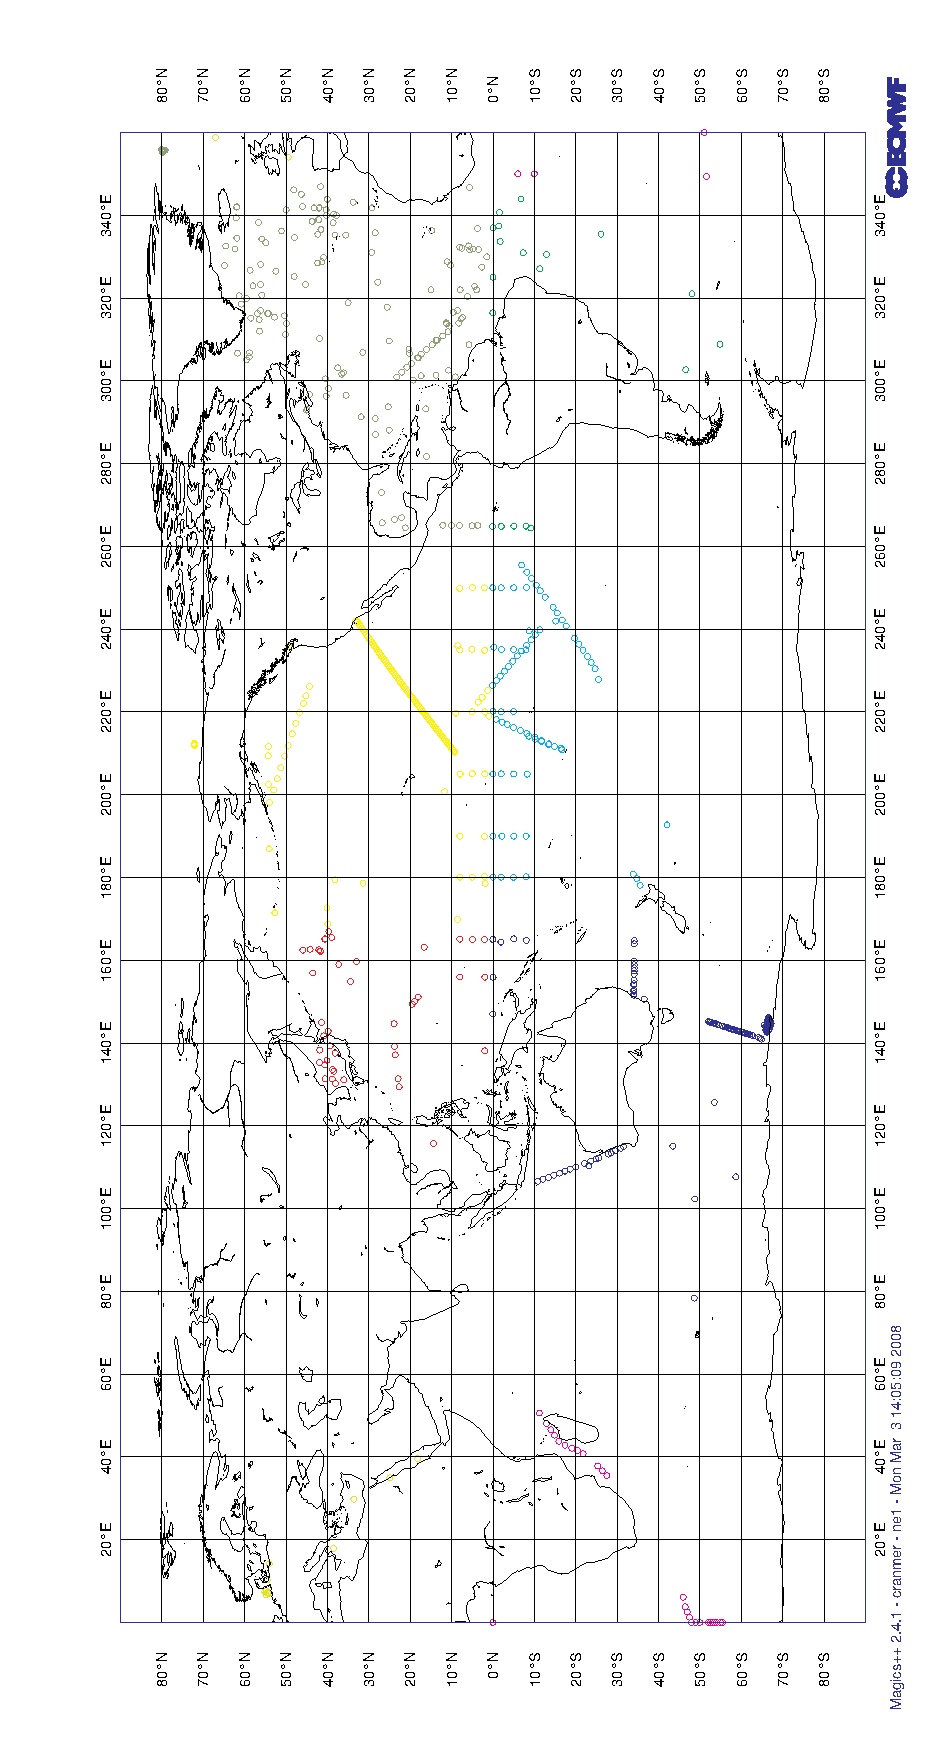
\includegraphics[width=10cm,height=12cm,angle=-90.]{./TexFiles/Figures/Fig_ASM_obsdist_local}
\caption{      \label{fig:obslocal}
Example of the distribution of observations with the geographical distribution of observational data.} 
\end{center}      \end{figure}
%>>>>>>>>>>>>>>>>>>>>>>>>>>>>

This is the simplest option in which the observations are distributed according 
to the domain of the grid-point parallelization. Figure~\ref{fig:obslocal}
shows an example of the distribution of the {\em in situ} data on processors 
with a different colour for each observation
on a given processor for a 4 $\times$ 2 decomposition with ORCA2. 
The grid-point domain decomposition is clearly visible on the plot.

The advantage of this approach is that all
information needed for horizontal interpolation is available without
any MPP communication. Of course, this is under the assumption that 
we are only using a $2 \times 2$ grid-point stencil for the interpolation 
(e.g., bilinear interpolation). For higher order interpolation schemes this
is no longer valid. A disadvantage with the above scheme is that the number of
observations on each processor can be very different. If the cost of
the actual interpolation is expensive relative to the communication of
data needed for interpolation, this could lead to load imbalance.

\subsubsection{Round-robin distribution of observations among processors}

%>>>>>>>>>>>>>>>>>>>>>>>>>>>>
\begin{figure}     \begin{center}
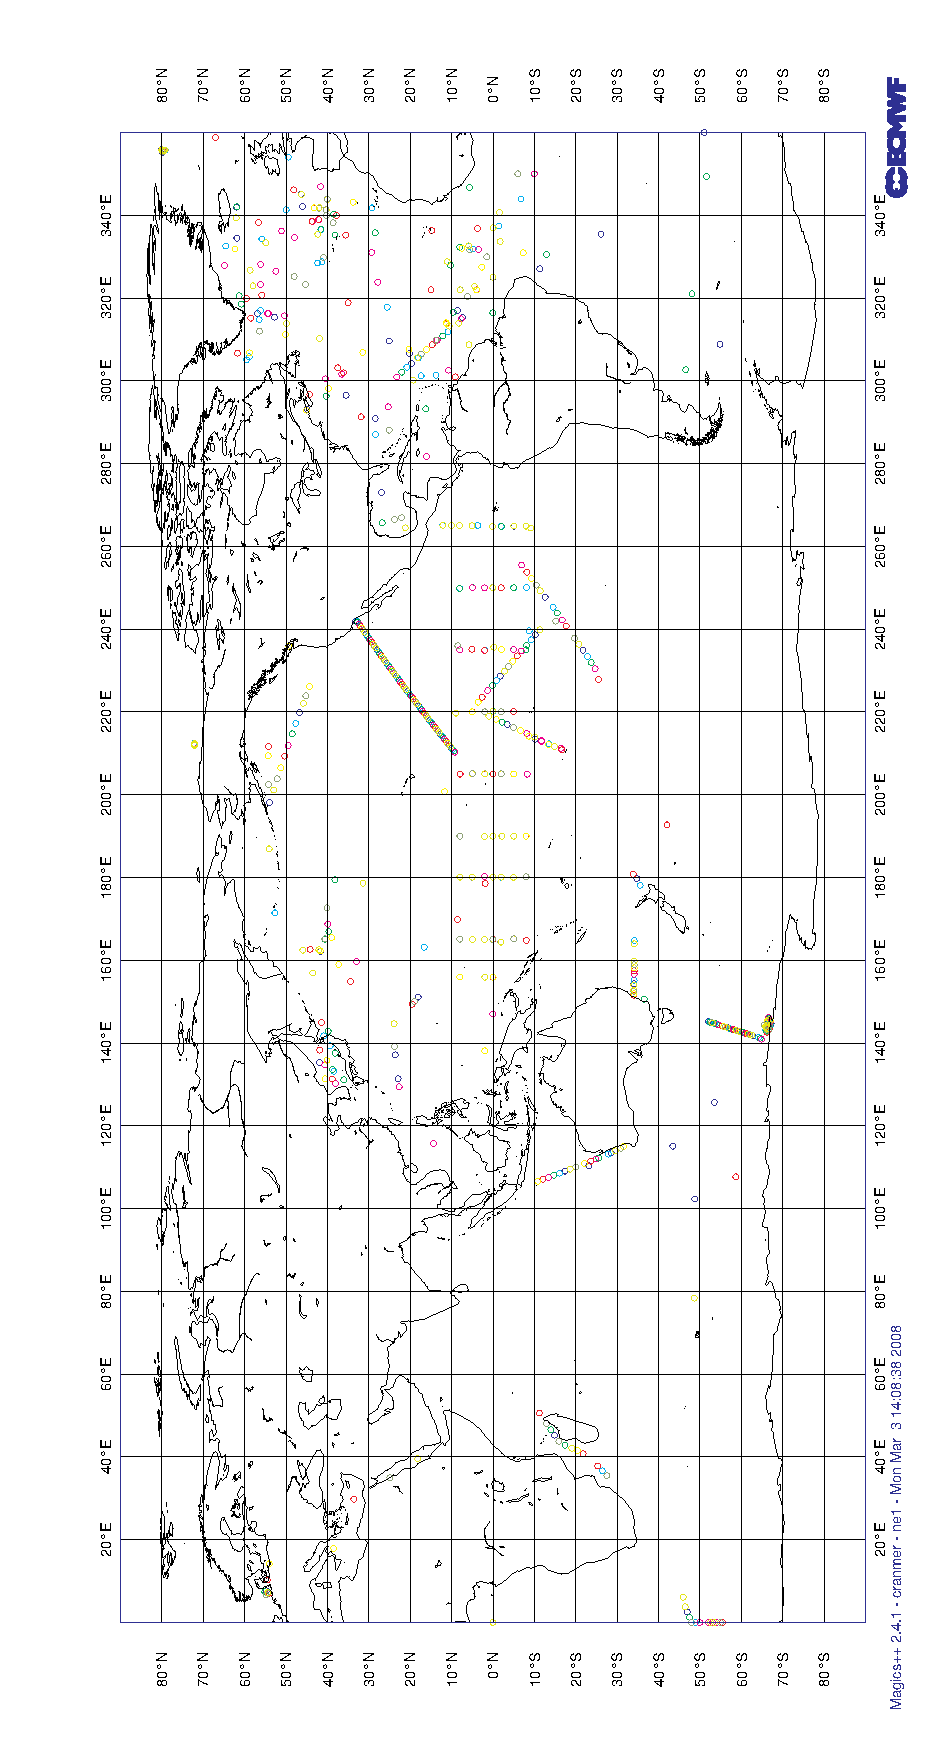
\includegraphics[width=10cm,height=12cm,angle=-90.]{./TexFiles/Figures/Fig_ASM_obsdist_global}
\caption{      \label{fig:obsglobal}
Example of the distribution of observations with the round-robin distribution of observational data.}
\end{center}     \end{figure}
%>>>>>>>>>>>>>>>>>>>>>>>>>>>>

An alternative approach is to distribute the observations equally
among processors and use message passing in order to retrieve 
the stencil for interpolation. The simplest distribution of the observations 
is to distribute them using a round-robin scheme. Figure~\ref{fig:obsglobal}
shows the distribution of the {\em in situ} data on processors for the
round-robin distribution of observations with a different colour for
each observation on a given processor for a 4 $\times$ 2 decomposition 
with ORCA2 for the same input data as in Fig.~\ref{fig:obslocal}.
The observations are now clearly randomly distributed on the globe.
In order to be able to perform horizontal interpolation in this case, 
a subroutine has been developed that retrieves any grid points in the 
global space.

\subsection{Vertical interpolation operator}

Vertical interpolation is achieved using either a cubic spline or
linear interpolation. For the cubic spline, the top and
bottom boundary conditions for the second derivative of the 
interpolating polynomial in the spline are set to zero.
At the bottom boundary, this is done using the land-ocean mask.

\newpage

% ================================================================
% Offline observation operator documentation
% ================================================================

%\usepackage{framed}

\section{Offline observation operator}
\label{OBS_ooo}

\subsection{Concept}

The obs oper maps model variables to observation space. It is possible to apply this mapping
without running the model. The software which performs this functionality is known as the
\textbf{offline obs oper}. The obs oper is divided into three stages. An initialisation phase,
an interpolation phase and an output phase. The implementation of which is outlined in the
previous sections. During the interpolation phase the offline obs oper populates the model
arrays by reading saved model fields from disk.

There are two ways of exploiting this offline capacity. The first is to mimic the behaviour of
the online system by supplying model fields at regular intervals between the start and the end
of the run. This approach results in a single model counterpart per observation. This kind of
usage produces feedback files the same file format as the online obs oper. 
The second is to take advantage of the offline setting in which multiple model counterparts can
be calculated per observation. In this case it is possible to consider all forecasts verifying
at the same time. By forecast, I mean any method which produces an estimate of physical reality
which is not an observed value. In the case of class 4 files this means forecasts, analyses, persisted
analyses and climatological values verifying at the same time. Although the class 4 file format
doesn't account for multiple ensemble members or multiple experiments per observation, it is possible
to include these components in the same or multiple files.

%--------------------------------------------------------------------------------------------------------
% offline_oper.exe 
%--------------------------------------------------------------------------------------------------------

\subsection{Using the offline observation operator}

\subsubsection{Building}

In addition to \emph{OPA\_SRC} the offline obs oper requires the inclusion
of the \emph{OOO\_SRC} directory. \emph{OOO\_SRC} contains a replacement \textbf{nemo.f90} and
\textbf{nemogcm.F90} which overwrites the resultant \textbf{nemo.exe}. This is the approach taken
by \emph{SAS\_SRC} and \emph{OFF\_SRC}.

%--------------------------------------------------------------------------------------------------------
% Running 
%--------------------------------------------------------------------------------------------------------
\subsubsection{Running}

The simplest way to use the executable is to edit and append the \textbf{ooo.nml} namelist to
a full NEMO namelist and then to run the executable as if it were nemo.exe. 

\subsubsection{Quick script}

A useful Python utility to control the namelist options can be found in \textbf{OBSTOOLS/OOO}. The
functions which locate model fields and observation files can be manually specified. The package
can be installed by appropriate use of the included setup.py script.

Documentation can be auto-generated by Sphinx by running \emph{make html} in the \textbf{doc} directory.

%--------------------------------------------------------------------------------------------------------
% Configuration section
%--------------------------------------------------------------------------------------------------------
\subsection{Configuring the offline observation operator}
The observation files and settings understood by \textbf{namobs} have been outlined in the online
obs oper section. In addition there are two further namelists wich control the operation of the offline
obs oper. \textbf{namooo} which controls the input model fields and \textbf{namcl4} which controls the
production of class 4 files. 

\subsubsection{Single field}

In offline mode model arrays are populated at appropriate time steps via input files.
At present, \textbf{tsn} and \textbf{sshn} are populated by the default read routines. 
These routines will be expanded upon in future versions to allow the specification of any
model variable. As such, input files must be global versions of the model domain with
\textbf{votemper}, \textbf{vosaline} and optionally \textbf{sshn} present.

For each field read there must be an entry in the \textbf{namooo} namelist specifying the
name of the file to read and the index along the \emph{time\_counter}. For example, to
read the second time counter from a single file the namelist would be.

\begin{alltt}
\tiny
\begin{verbatim} 
!----------------------------------------------------------------------
!       namooo Offline obs_oper namelist
!----------------------------------------------------------------------
!   ooo_files    specifies the files containing the model counterpart
!   nn_ooo_idx   specifies the time_counter index within the model file
&namooo
   ooo_files = "foo.nc"
   nn_ooo_idx = 2
/
\end{verbatim} 
\end{alltt}

\subsubsection{Multiple fields per run}

Model field iteration is controlled via \textbf{nn\_ooo\_freq} which specifies
the number of model steps at which the next field gets read. For example, if
12 hourly fields are to be interpolated in a setup where 288 steps equals 24 hours.

\begin{alltt}
\tiny
\begin{verbatim} 
!----------------------------------------------------------------------
!       namooo Offline obs_oper namelist
!----------------------------------------------------------------------
!   ooo_files    specifies the files containing the model counterpart
!   nn_ooo_idx   specifies the time_counter index within the model file
!   nn_ooo_freq  specifies number of time steps between read operations
&namooo
   ooo_files = "foo.nc" "foo.nc"
   nn_ooo_idx = 1 2
   nn_ooo_freq = 144
/
\end{verbatim} 
\end{alltt}

The above namelist will result in feedback files whose first 12 hours contain
the first field of foo.nc and the second 12 hours contain the second field.

%\begin{framed}
\textbf{Note} Missing files can be denoted as "nofile".
%\end{framed}

It is easy to see how a collection of fields taken fron a number of files 
at different indices can be combined at a particular frequency in time to 
generate a pseudo model evolution. As long as all that is needed is a single
model counterpart at a regular interval then namooo is all that needs to
be edited. However, a far more interesting approach can be taken in which
multiple forecasts, analyses, persisted analyses and climatologies are
considered against the same set of observations. For this a slightly more
complicated approach is needed. It is referred to as \emph{Class 4} since
it is the fourth metric defined by the GODAE intercomparison project.

%--------------------------------------------------------------------------------------------------------
% Class 4 file section
%--------------------------------------------------------------------------------------------------------
\subsubsection{Multiple model counterparts per observation a.k.a Class 4}

A generalisation of feedback files to allow multiple model components per observation. For a single
observation, as well as previous forecasts verifying at the same time there are also analyses, persisted
analyses and climatologies. 


The above namelist performs two basic functions. It organises the fields
given in \textbf{namooo} into groups so that observations can be matched
up multiple times. It also controls the metadata and the output variable
of the class 4 file when a write routine is called.

%\begin{framed}
\textbf{Note: ln\_cl4} must be set to \emph{.TRUE.} in \textbf{namobs} 
to use class 4 outputs.
%\end{framed}

\subsubsection{Class 4 naming convention}

The standard class 4 file naming convention is as follows.

\noindent
\linebreak
\textbf{\$\{prefix\}\_\$\{yyyymmdd\}\_\$\{sys\}\_\$\{cfg\}\_\$\{vn\}\_\$\{kind\}\_\$\{nproc\}.nc}

\noindent
\linebreak
Much of the namelist is devoted to specifying this convention. The
following namelist settings control the elements of the output
file names. Each should be specified as a single string of character data.

\begin{description}
\item[cl4\_prefix]
Prefix for class 4 files e.g. class4
\item[cl4\_date]
YYYYMMDD validity date
\item[cl4\_sys]
The name of the class 4 model system e.g. FOAM
\item[cl4\_cfg]
The name of the class 4 model configuration e.g. orca025
\item[cl4\_vn]
The name of the class 4 model version e.g. 12.0
\end{description}

\noindent
The kind is specified by the observation type internally to the obs oper. The processor
number is specified internally in NEMO. 

\subsubsection{Class 4 file global attributes}

Global attributes necessary to fulfill the class 4 file definition. These
are also useful pieces of information when collaborating with external
partners.

\begin{description}
\item[cl4\_contact]
Contact email for class 4 files.
\item[cl4\_inst]
The name of the producers institution.
\item[cl4\_cfg]
The name of the class 4 model configuration e.g. orca025
\item[cl4\_vn]
The name of the class 4 model version e.g. 12.0
\end{description}

\noindent
The obs\_type,
creation date and validity time are specified internally to the obs oper.

\subsubsection{Class 4 model counterpart configuration}

As seen previously it is possible to perform a single sweep of the
obs oper and specify a collection of model fields equally spaced 
along that sweep. In the class 4 case the single sweep is replaced
with multiple sweeps and a certain ammount of book keeping is
needed to ensure each model counterpart makes its way to the 
correct piece of memory in the output files.

\noindent
\linebreak
In terms of book keeping, the offline obs oper needs to know how many
full sweeps need to be performed. This is specified via the 
\textbf{cl4\_match\_len} variable and is the total number of model
counterparts per observation. For example, a 3 forecasts plus 3 persistence
fields plus an analysis field would be 7 counterparts per observation.

\begin{alltt}
\tiny
\begin{verbatim}
   cl4_match_len = 7
\end{verbatim}
\end{alltt}

Then to correctly allocate a class 4 file the forecast axis must be defined. This
is controlled via \textbf{cl4\_fcst\_len}, which in out above example would be 3.

\begin{alltt}
\tiny
\begin{verbatim}
   cl4_fcst_len = 3
\end{verbatim}
\end{alltt}

Then for each model field it is necessary to designate what class 4 variable and
index along the forecast dimension the model counterpart should be stored in the
output file. As well as a value for that lead time in hours, this will be useful
when interpreting the data afterwards. 

\begin{alltt}
\tiny
\begin{verbatim}
   cl4_vars = "forecast" "forecast" "forecast" "persistence" "persistence"
              "persistence" "best_estimate"
   cl4_fcst_idx = 1 2 3 1 2 3 1
   cl4_leadtime = 12 36 60 
\end{verbatim}
\end{alltt}

In terms of files and indices of fields inside each file the class 4 approach
makes use of the \textbf{namooo} namelist. If our fields are in separate files
with a single field per file our example inputs will be specified.

\begin{alltt}
\tiny
\begin{verbatim}
   ooo_files = "F.1.nc" "F.2.nc" "F.3.nc" "P.1.nc" "P.2.nc" "P.3.nc" "A.1.nc"
   nn_ooo_idx = 1 1 1 1 1 1 1
\end{verbatim}
\end{alltt}

When we combine all of the naming conventions, global attributes and i/o instructions
the class 4 namelist becomes.

\begin{alltt}
\tiny
\begin{verbatim}
!----------------------------------------------------------------------
!       namooo Offline obs_oper namelist
!----------------------------------------------------------------------
!   ooo_files    specifies the files containing the model counterpart
!   nn_ooo_idx   specifies the time_counter index within the model file
!   nn_ooo_freq  specifies number of time steps between read operations
&namooo
   ooo_files = "F.1.nc" "F.2.nc" "F.3.nc" "P.1.nc" "P.2.nc" "P.3.nc" "A.1.nc"
   nn_ooo_idx = 1 1 1 1 1 1 1
/
!----------------------------------------------------------------------
!       namcl4 Offline obs_oper class 4 namelist
!----------------------------------------------------------------------
!
!  Naming convention
!  -----------------
!  cl4_prefix    specifies the output file prefix
!  cl4_date      specifies the output file validity date
!  cl4_sys       specifies the model counterpart system
!  cl4_cfg       specifies the model counterpart configuration
!  cl4_vn        specifies the model counterpart version
!  cl4_inst      specifies the model counterpart institute
!  cl4_contact   specifies the file producers contact details
!
!  I/O specification
!  -----------------
!  cl4_vars      specifies the names of the output file netcdf variable
!  cl4_fcst_idx  specifies output file forecast index
!  cl4_fcst_len  specifies forecast axis length
!  cl4_match_len specifies number of unique matches per observation
!  cl4_leadtime  specifies the forecast axis lead time 
!
&namcl4
   cl4_match_len = 7
   cl4_fcst_len = 3
   cl4_fcst_idx = 1 2 3 1 2 3 1
   cl4_vars = "forecast" "forecast" "forecast" "persistence" "persistence"
              "persistence" "best_estimate"
   cl4_leadtime = 12 36 60
   cl4_prefix = "class4"
   cl4_date = "20130101"
   cl4_vn = "12.0"
   cl4_sys = "FOAM"
   cl4_cfg = "AMM7"
   cl4_contact = "example@example.com"
   cl4_inst = "UK Met Office"
/
\end{verbatim}
\end{alltt}

\subsubsection{Climatology interpolation}

The climatological counterpart is generated at the start of the run by restarting 
the model from climatology through appropriate use of \textbf{namtsd}. To override
the offline observation operator read routine and to take advantage of the restart
settings, specify the first entry in \textbf{cl4\_vars} as "climatology". This will then
pipe the restart from climatology into the output class 4 file. As in every other
class 4 matchup the input file, input index and output index must be specified.
These can be replaced with dummy data since they are not used but they must be
present to cycle through the matchups correctly. 

\subsection{Advanced usage}

In certain cases it may be desirable to include both multiple model fields per
observation window with multiple match ups per observation. This can be achieved
by specifying \textbf{nn\_ooo\_freq} as well as the class 4 settings. Care must
be taken in generating the ooo\_files list such that the files are arranged into
consecutive blocks of single match ups. For example, 2 forecast fields 
of 12 hourly data would result in 4 separate read operations but only 2 write
operations, 1 per forecast.

\begin{alltt}
\tiny
\begin{verbatim}
   ooo_files = "F1.nc" "F1.nc" "F2.nc" "F2.nc"
...
   cl4_fcst_idx = 1 2
\end{verbatim}
\end{alltt}

The above notation reveals the internal split between match up iterators and file
iterators. This technique has not been used before so experimentation is needed
before results can be trusted.




\newpage

\section{Observation Utilities}
\label{OBS_obsutils}

Some tools for viewing and processing of observation and feedback files are provided in the
NEMO repository for convenience. These include OBSTOOLS which are a collection of Fortran
programs which are helpful to deal with feedback files. They do such tasks as observation file
conversion, printing of file contents, some basic statistical analysis of feedback files. The
other tool is an IDL program called dataplot which uses a graphical interface to visualise
observations and feedback files. OBSTOOLS and dataplot are described in more detail below.  

\subsection{Obstools}

A series of Fortran utilities is provided with NEMO called OBSTOOLS. This are helpful in
handling observation files and the feedback file output from the NEMO observation operator.
The utilities are as follows

\subsubsection{c4comb}

The program c4comb combines multiple class 4 files produced by individual processors in an
MPI run of NEMO offline obs\_oper into a single class 4 file. The program is called in the following way:

\begin{alltt}
\footnotesize
\begin{verbatim}
c4comb.exe outputfile inputfile1 inputfile2 ...
\end{verbatim}
\end{alltt}

\subsubsection{corio2fb}

The program corio2fb converts profile observation files from the Coriolis format to the
standard feedback format. The program is called in the following way:

\begin{alltt}
\footnotesize
\begin{verbatim}
corio2fb.exe outputfile inputfile1 inputfile2 ...
\end{verbatim}
\end{alltt}

\subsubsection{enact2fb}

The program enact2fb converts profile observation files from the ENACT format to the standard
feedback format. The program is called in the following way:

\begin{alltt}
\footnotesize
\begin{verbatim}
enact2fb.exe outputfile inputfile1 inputfile2 ...
\end{verbatim}
\end{alltt}

\subsubsection{fbcomb}

The program fbcomb combines multiple feedback files produced by individual processors in an
MPI run of NEMO into a single feedback file. The program is called in the following way:

\begin{alltt}
\footnotesize
\begin{verbatim}
fbcomb.exe outputfile inputfile1 inputfile2 ...
\end{verbatim}
\end{alltt}

\subsubsection{fbmatchup}

The program fbmatchup will match observations from two feedback files. The program is called
in the following way:

\begin{alltt}
\footnotesize
\begin{verbatim}
fbmatchup.exe outputfile inputfile1 varname1 inputfile2 varname2 ...
\end{verbatim}
\end{alltt}


\subsubsection{fbprint}

The program fbprint will print the contents of a feedback file or files to standard output.
Selected information can be output using optional arguments. The program is called in the
following way:

\begin{alltt}
\footnotesize
\begin{verbatim}
fbprint.exe [options] inputfile

options:
     -b            shorter output
     -q            Select observations based on QC flags
     -Q            Select observations based on QC flags
     -B            Select observations based on QC flags
     -u            unsorted
     -s ID         select station ID  
     -t TYPE       select observation type
     -v NUM1-NUM2  select variable range to print by number 
                      (default all)
     -a NUM1-NUM2  select additional variable range to print by number 
                      (default all)
     -e NUM1-NUM2  select extra variable range to print by number 
                      (default all)
     -d            output date range
     -D            print depths
     -z            use zipped files
\end{verbatim}
\end{alltt}

\subsubsection{fbsel}

The program fbsel will select or subsample observations. The program is called in the
following way:

\begin{alltt}
\footnotesize
\begin{verbatim}
fbsel.exe <input filename> <output filename>
\end{verbatim}
\end{alltt}

\subsubsection{fbstat}

The program fbstat will output summary statistics in different global areas into a number of
files. The program is called in the following way:

\begin{alltt}
\footnotesize
\begin{verbatim}
fbstat.exe [-nmlev] <filenames>
\end{verbatim}
\end{alltt}

\subsubsection{fbthin}

The program fbthin will thin the data to 1 degree resolution. The code could easily be
modified to thin to a different resolution. The program is called in the following way:

\begin{alltt}
\footnotesize
\begin{verbatim}
fbthin.exe inputfile outputfile
\end{verbatim}
\end{alltt}

\subsubsection{sla2fb}

The program sla2fb will convert an AVISO SLA format file to feedback format. The program is
called in the following way:

\begin{alltt}
\footnotesize
\begin{verbatim}
sla2fb.exe [-s type] outputfile inputfile1 inputfile2 ...

Option:
     -s            Select altimeter data_source
\end{verbatim}
\end{alltt}

\subsubsection{vel2fb}

The program vel2fb will convert TAO/PIRATA/RAMA currents files to feedback format. The program
is called in the following way:

\begin{alltt}
\footnotesize
\begin{verbatim}
vel2fb.exe outputfile inputfile1 inputfile2 ...
\end{verbatim}
\end{alltt}

\subsection{building the obstools}

To build the obstools use in the tools directory use ./maketools -n OBSTOOLS -m [ARCH].

\subsection{Dataplot}

An IDL program called dataplot is included which uses a graphical interface to visualise
observations and feedback files. It is possible to zoom in, plot individual profiles and
calculate some basic statistics. To plot some data run IDL and then:
\begin{alltt}
\footnotesize
\begin{verbatim}
IDL> dataplot, "filename"
\end{verbatim}
\end{alltt}

To read multiple files into dataplot, for example multiple feedback files from different
processors or from different days, the easiest method is to use the spawn command to generate
a list of files which can then be passed to dataplot.
\begin{alltt}
\footnotesize
\begin{verbatim}
IDL> spawn, 'ls profb*.nc', files
IDL> dataplot, files
\end{verbatim}
\end{alltt}

Fig~\ref{fig:obsdataplotmain} shows the main window which is launched when dataplot starts.
This is split into three parts. At the top there is a menu bar which contains a variety of
drop down menus. Areas - zooms into prespecified regions; plot - plots the data as a
timeseries or a T-S diagram if appropriate; Find - allows data to be searched; Config - sets
various configuration options.

The middle part is a plot of the geographical location of the observations. This will plot the
observation value, the model background value or observation minus background value depending
on the option selected in the radio button at the bottom of the window. The plotting colour
range can be changed by clicking on the colour bar. The title of the plot gives some basic
information about the date range and depth range shown, the extreme values, and the mean and
rms values. It is possible to zoom in using a drag-box. You may also zoom in or out using the
mouse wheel.

The bottom part of the window controls what is visible in the plot above. There are two bars
which select the level range plotted (for profile data). The other bars below select the date
range shown. The bottom of the figure allows the option to plot the mean, root mean square,
standard deviation or mean square values. As mentioned above you can choose to plot the
observation value, the model background value or observation minus background value. The next
group of radio buttons selects the map projection. This can either be regular latitude
longitude grid, or north or south polar stereographic. The next group of radio buttons will
plot bad observations, switch to salinity and plot density for profile observations. The
rightmost group of buttons will print the plot window as a postscript, save it as png, or exit
from dataplot.

%>>>>>>>>>>>>>>>>>>>>>>>>>>>>
\begin{figure}     \begin{center}
%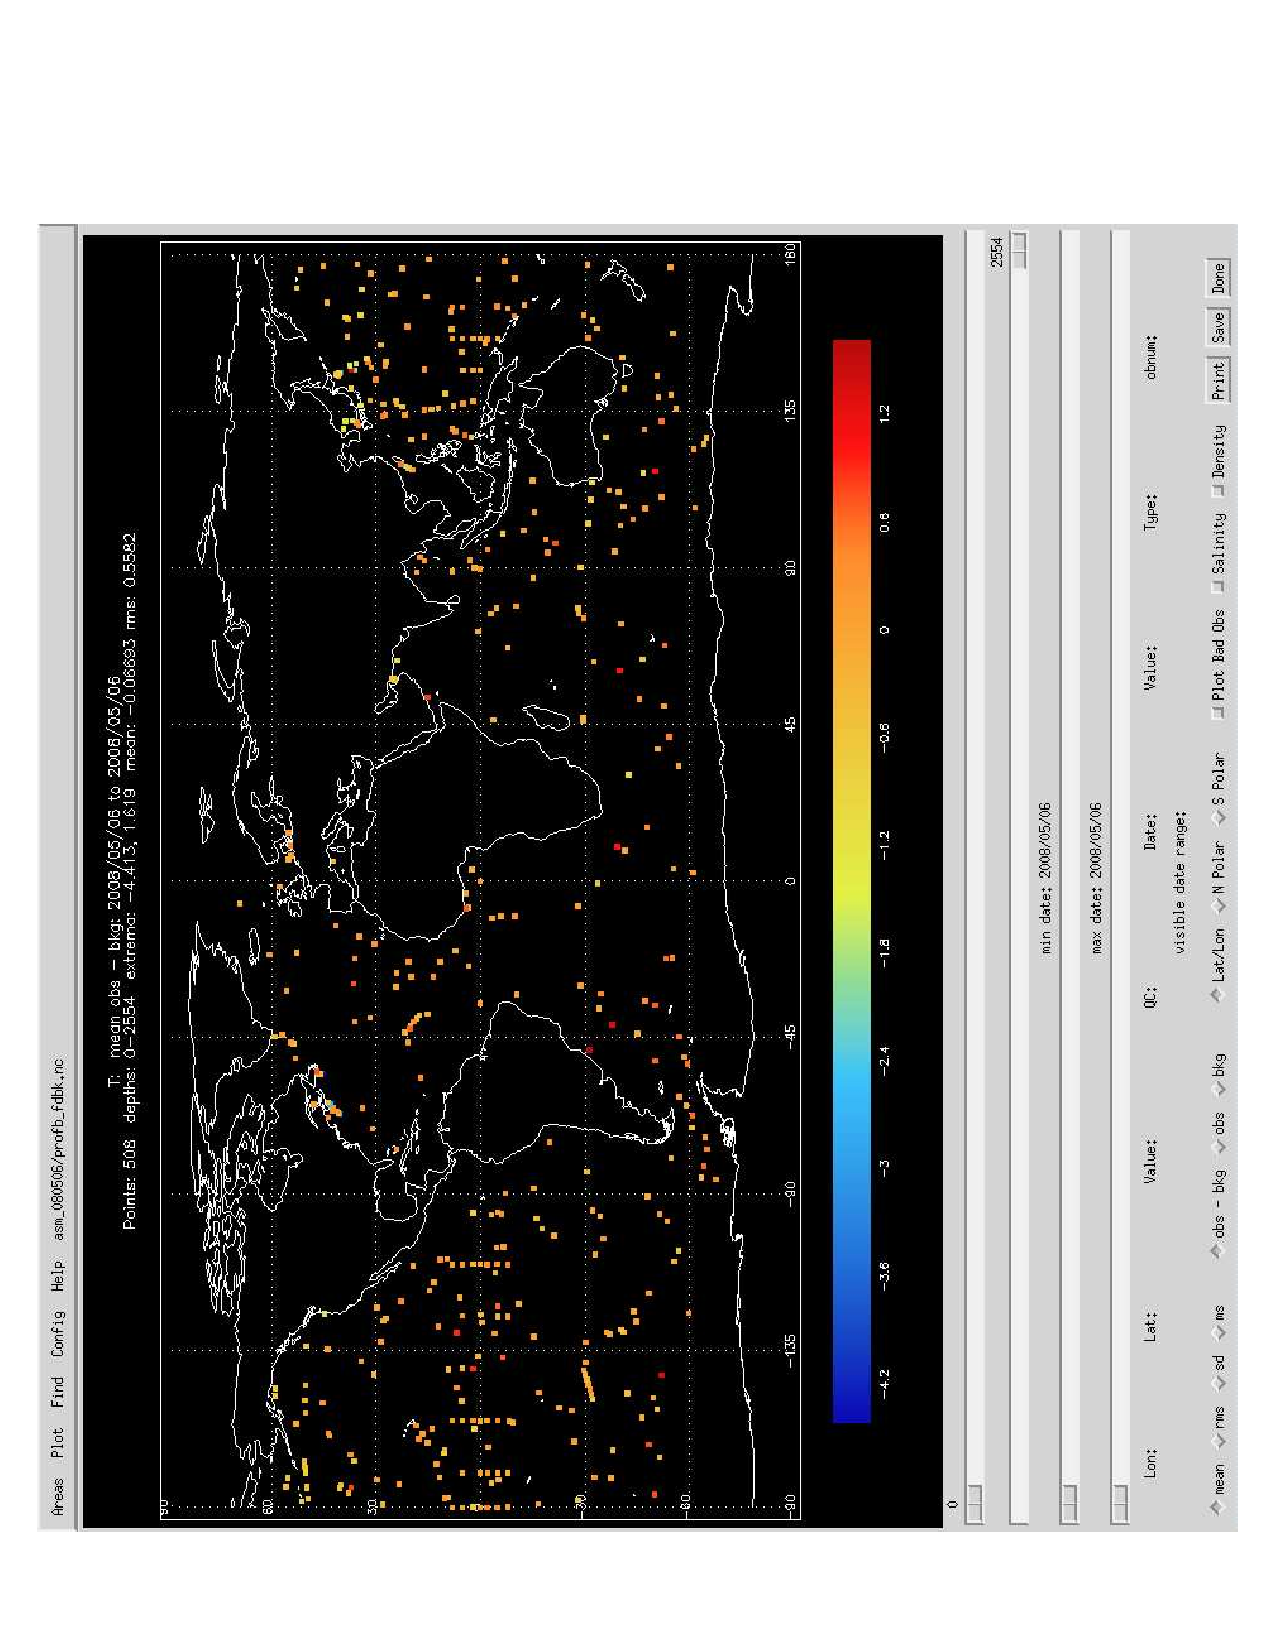
\includegraphics[width=10cm,height=12cm,angle=-90.]{./TexFiles/Figures/Fig_OBS_dataplot_main}
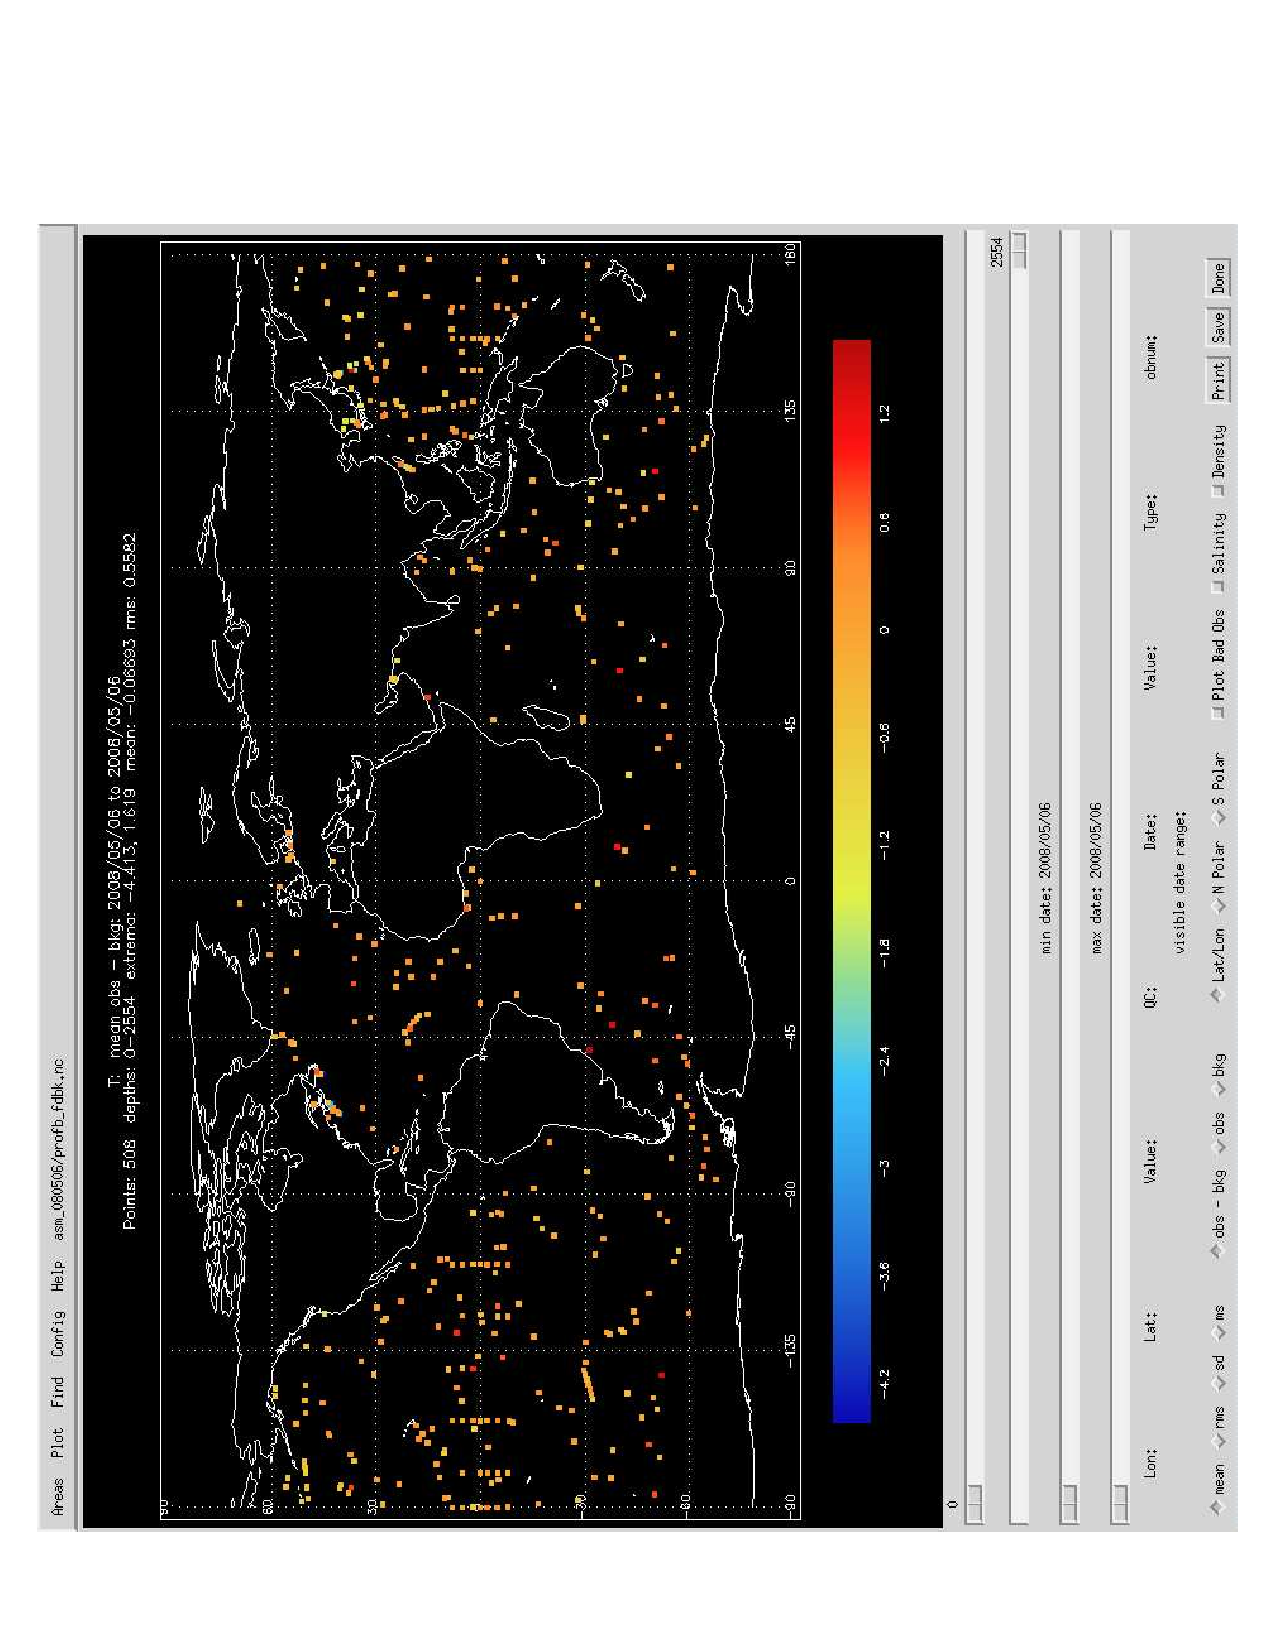
\includegraphics[width=9cm,angle=-90.]{./TexFiles/Figures/Fig_OBS_dataplot_main}
\caption{      \label{fig:obsdataplotmain}
Main window of dataplot.}
\end{center}     \end{figure}
%>>>>>>>>>>>>>>>>>>>>>>>>>>>>

If a profile point is clicked with the mouse button a plot of the observation and background
values as a function of depth (Fig~\ref{fig:obsdataplotprofile}).

%>>>>>>>>>>>>>>>>>>>>>>>>>>>>
\begin{figure}     \begin{center}
%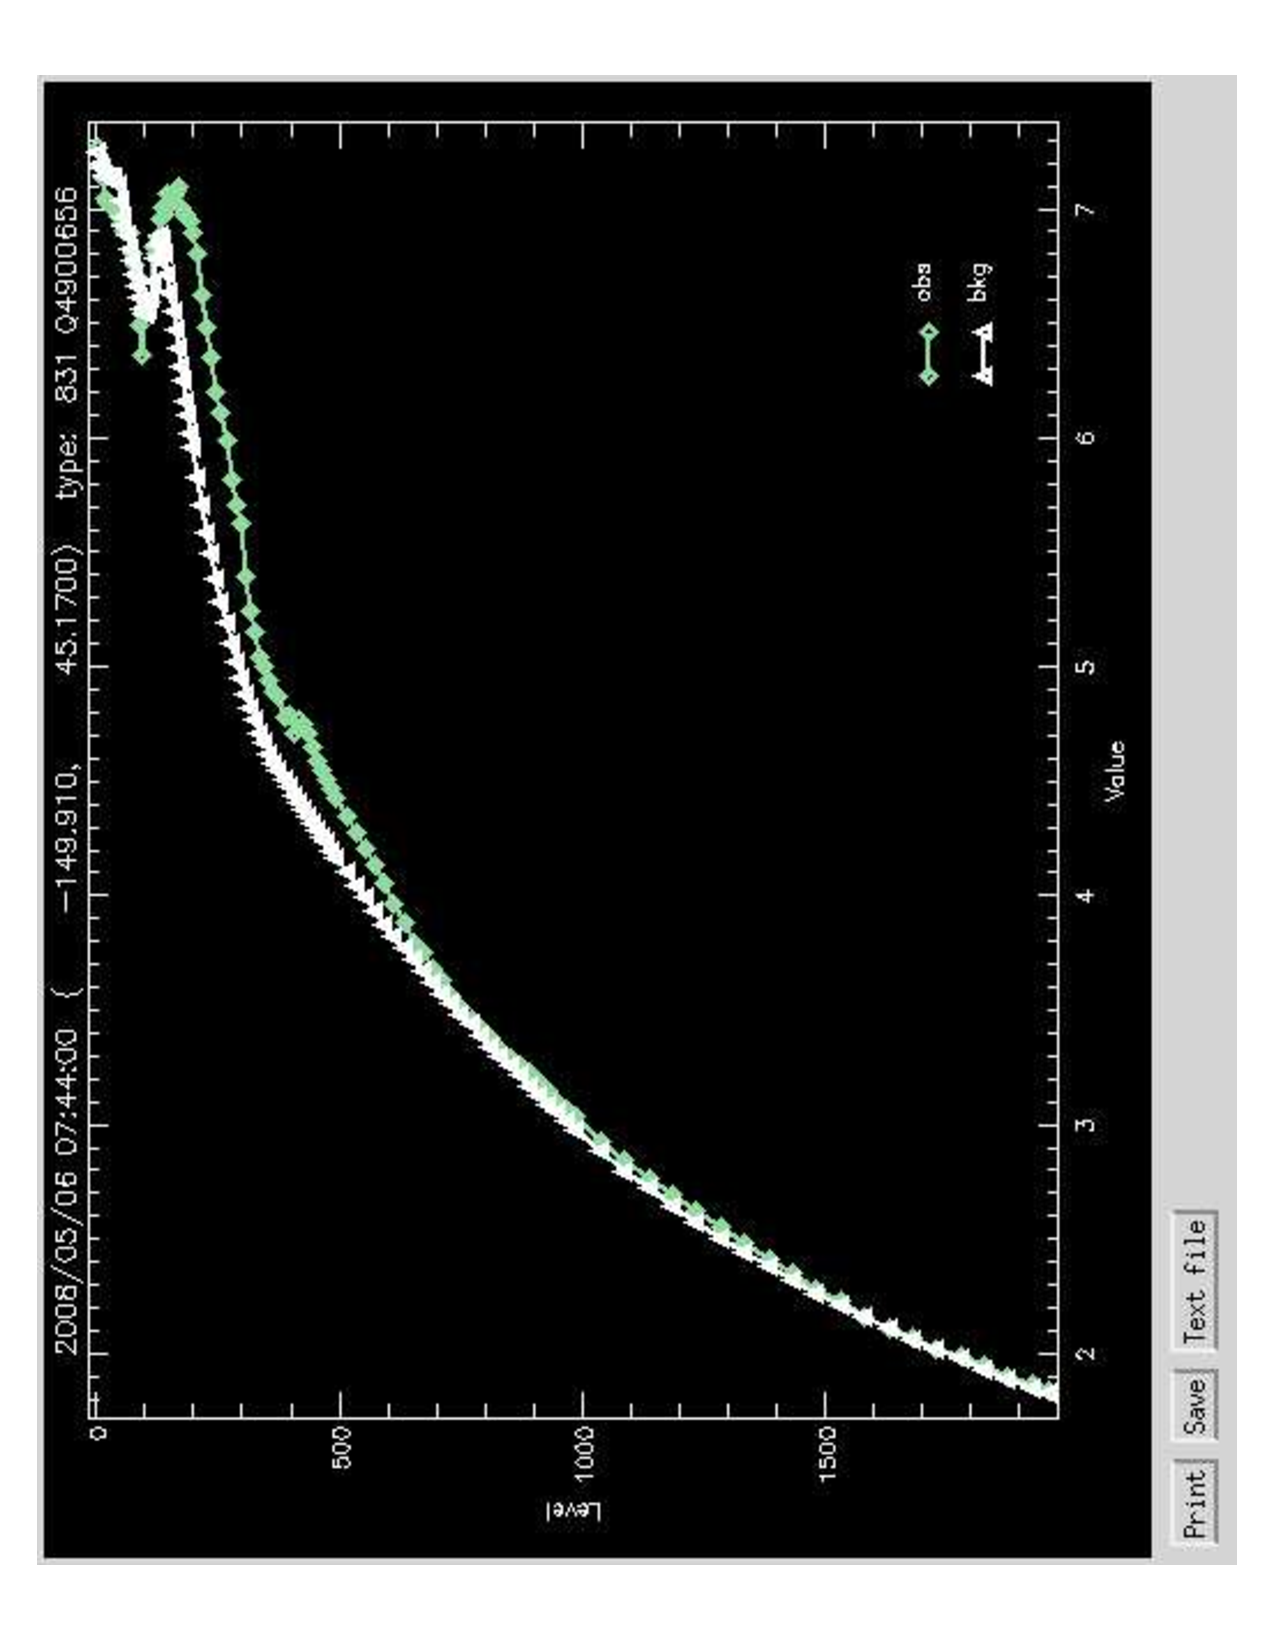
\includegraphics[width=10cm,height=12cm,angle=-90.]{./TexFiles/Figures/Fig_OBS_dataplot_prof}
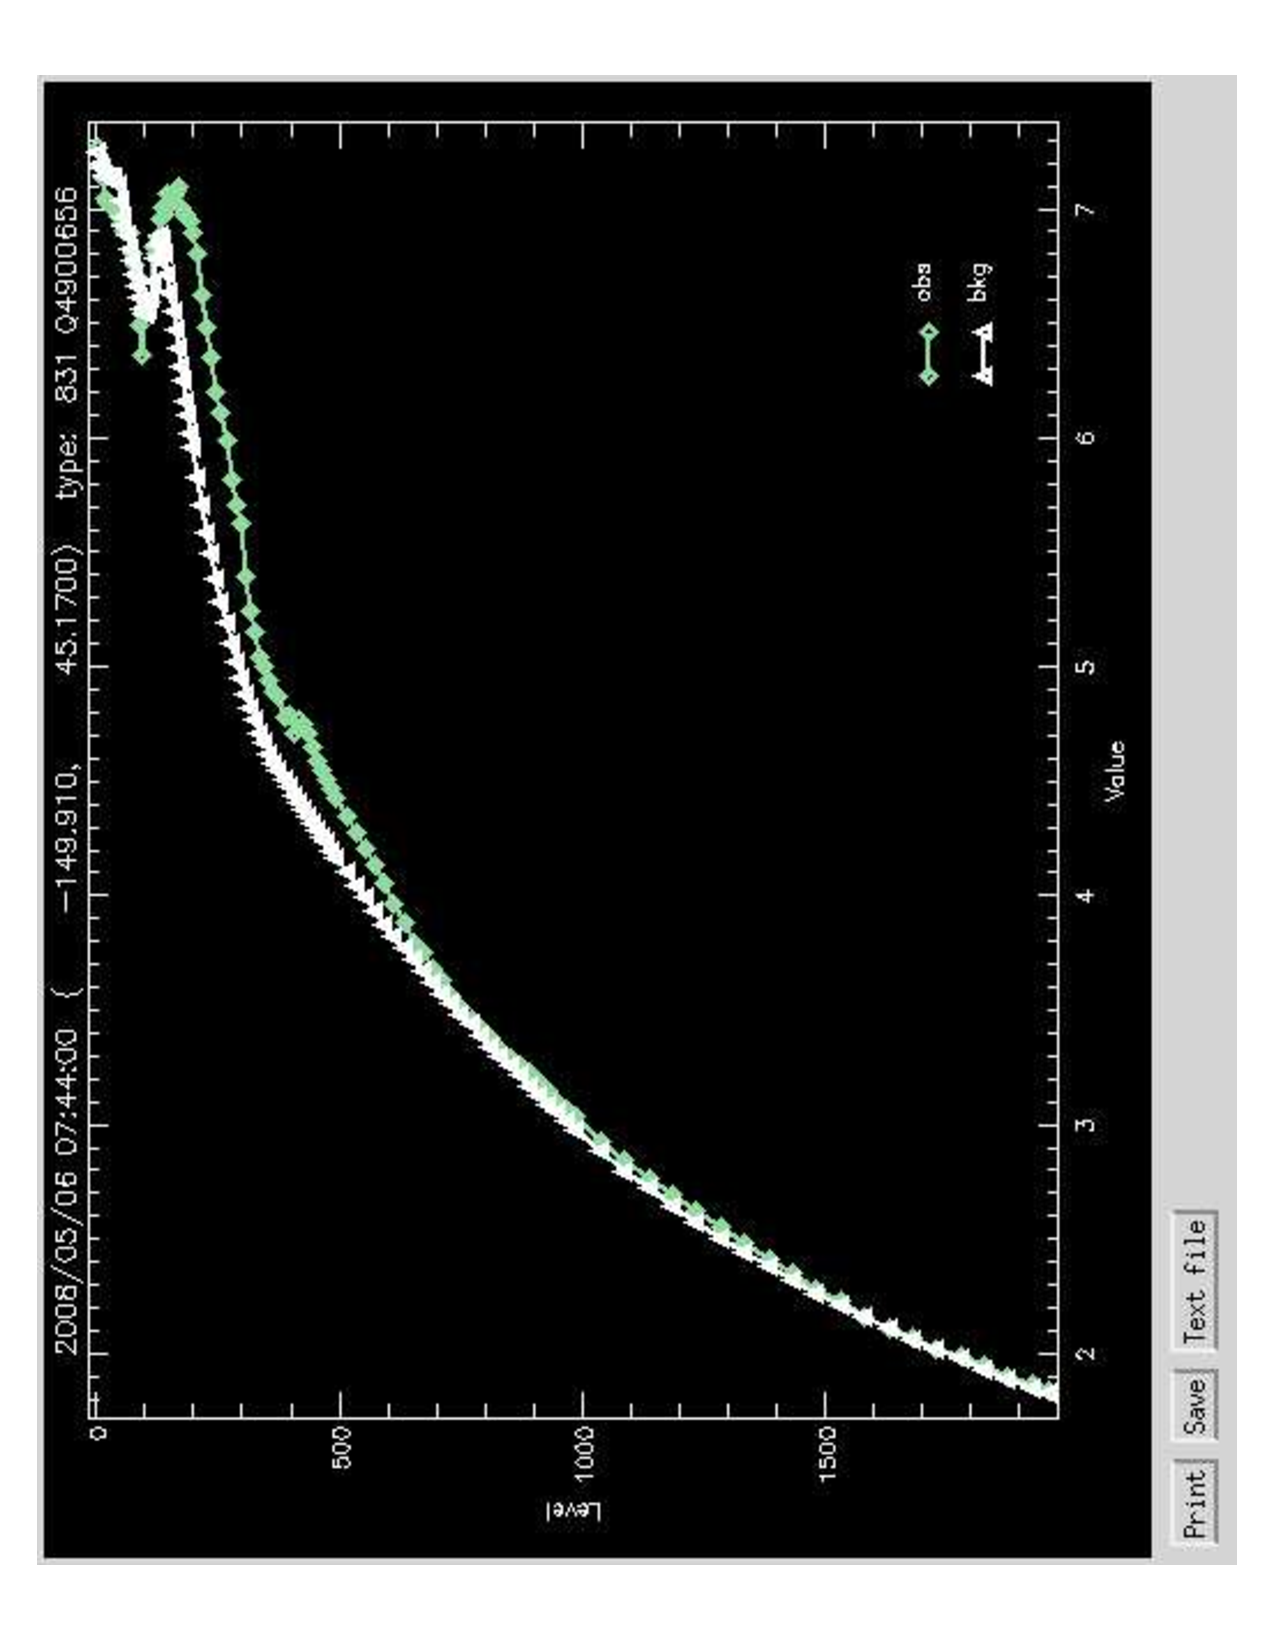
\includegraphics[width=7cm,angle=-90.]{./TexFiles/Figures/Fig_OBS_dataplot_prof}
\caption{      \label{fig:obsdataplotprofile}
Profile plot from dataplot produced by right clicking on a point in the main window.}
\end{center}     \end{figure}
%>>>>>>>>>>>>>>>>>>>>>>>>>>>>




          % Observation operator

% ================================================================
% Chapter Assimilation increments (ASM)
% ================================================================
\chapter{Apply assimilation increments (ASM)}
\label{ASM}

Authors: D. Lea,  M. Martin, K. Mogensen, A. Weaver, ...   % do we keep

\minitoc


\newpage
$\ $\newline    % force a new line

The ASM code adds the functionality to apply increments to the model variables: 
temperature, salinity, sea surface height, velocity and sea ice concentration. 
These are read into the model from a NetCDF file which may be produced by separate data
assimilation code.  The code can also output model background fields which are used
as an input to data assimilation code. This is all controlled by the namelist
\textit{\ngn{nam\_asminc} }.  There is a brief description of all the namelist options
provided.  To build the ASM code \key{asminc} must be set.

%===============================================================

\section{Direct initialization}
\label{ASM_DI}

Direct initialization (DI) refers to the instantaneous correction
of the model background state using the analysis increment.
DI is used when \np{ln\_asmdin} is set to true.

\section{Incremental Analysis Updates}
\label{ASM_IAU}

Rather than updating the model state directly with the analysis increment,
it may be preferable to introduce the increment gradually into the ocean
model in order to minimize spurious adjustment processes. This technique
is referred to as Incremental Analysis Updates (IAU) \citep{Bloom_al_MWR96}.
IAU is a common technique used with 3D assimilation methods such as 3D-Var or OI.
IAU is used when \np{ln\_asmiau} is set to true.

With IAU, the model state trajectory ${\bf x}$ in the assimilation window 
($t_{0} \leq t_{i} \leq t_{N}$)
is corrected by adding the analysis increments for temperature, salinity, horizontal velocity and SSH
as additional tendency terms to the prognostic equations:
\begin{eqnarray}     \label{eq:wa_traj_iau}
{\bf x}^{a}(t_{i}) = M(t_{i}, t_{0})[{\bf x}^{b}(t_{0})] 
\; + \; F_{i} \delta \tilde{\bf x}^{a} 
\end{eqnarray}
where $F_{i}$ is a weighting function for applying the increments $\delta
\tilde{\bf x}^{a}$ defined such that $\sum_{i=1}^{N} F_{i}=1$.
${\bf x}^b$ denotes the model initial state and ${\bf x}^a$ is the model state
after the increments are applied. 
To control the adjustment time of the model to the increment,
the increment can be applied over an arbitrary sub-window,
$t_{m} \leq t_{i} \leq t_{n}$, of the main assimilation window,
where $t_{0} \leq t_{m} \leq t_{i}$ and $t_{i} \leq t_{n} \leq t_{N}$,
Typically the increments are spread evenly over the full window.
In addition, two different weighting functions have been implemented.
The first function employs constant weights, 
\begin{eqnarray}    \label{eq:F1_i}
F^{(1)}_{i}
=\left\{ \begin{array}{ll}
   0     &    {\rm if} \; \; \; t_{i} < t_{m}                \\
   1/M &    {\rm if} \; \; \; t_{m} < t_{i} \leq t_{n} \\
   0     &    {\rm if} \; \; \; t_{i} > t_{n}
  \end{array} \right. 
\end{eqnarray}
where $M = m-n$.
The second function employs peaked hat-like weights in order to give maximum 
weight in the centre of the sub-window, with the weighting reduced 
linearly to a small value at the window end-points:
\begin{eqnarray}     \label{eq:F2_i}
F^{(2)}_{i}
=\left\{ \begin{array}{ll}
   0                           &    {\rm if} \; \; \; t_{i}       <     t_{m}                        \\
   \alpha \, i               &    {\rm if} \; \; \; t_{m}    \leq t_{i}    \leq   t_{M/2}   \\
   \alpha \, (M - i +1) &    {\rm if} \; \; \; t_{M/2}  <    t_{i}    \leq   t_{n}       \\
   0                            &   {\rm if} \; \; \; t_{i}        >    t_{n}
  \end{array} \right.
\end{eqnarray}
where $\alpha^{-1} = \sum_{i=1}^{M/2} 2i$ and $M$ is assumed to be even. 
The weights described by \eqref{eq:F2_i} provide a 
smoother transition of the analysis trajectory from one assimilation cycle 
to the next than that described by \eqref{eq:F1_i}.

%==========================================================================
% Divergence damping description %%%
\section{Divergence damping initialisation}
\label{ASM_details}

The velocity increments may be initialized by the iterative application of 
a divergence damping operator. In iteration step $n$ new estimates of 
velocity increments $u^{n}_I$ and $v^{n}_I$ are updated by:
\begin{equation} \label{eq:asm_dmp}
\left\{ \begin{aligned}
 u^{n}_I = u^{n-1}_I + \frac{1}{e_{1u} } \delta _{i+1/2} \left( {A_D
\;\chi^{n-1}_I } \right) \\
\\
 v^{n}_I = v^{n-1}_I + \frac{1}{e_{2v} } \delta _{j+1/2} \left( {A_D
\;\chi^{n-1}_I } \right) \\
\end{aligned} \right.,
\end{equation}
where
\begin{equation} \label{eq:asm_div}
\chi^{n-1}_I = \frac{1}{e_{1t}\,e_{2t}\,e_{3t} }
                \left( {\delta _i \left[ {e_{2u}\,e_{3u}\,u^{n-1}_I} \right]
                       +\delta _j \left[ {e_{1v}\,e_{3v}\,v^{n-1}_I} \right]} \right).
\end{equation}
By the application of \eqref{eq:asm_dmp} and \eqref{eq:asm_dmp} the divergence is filtered
in each iteration, and the vorticity is left unchanged. In the presence of coastal boundaries
with zero velocity increments perpendicular to the coast the divergence is strongly damped.
This type of the initialisation reduces the vertical velocity magnitude  and alleviates the
problem of the excessive unphysical vertical mixing in the first steps of the model 
integration \citep{Talagrand_JAS72, Dobricic_al_OS07}. Diffusion coefficients are defined as 
$A_D = \alpha e_{1t} e_{2t}$, where $\alpha = 0.2$. The divergence damping is activated by
assigning to \np{nn\_divdmp} in the \textit{nam\_asminc} namelist a value greater than zero. 
By choosing this value to be of the order of 100 the increments in the vertical velocity will 
be significantly reduced.


%==========================================================================

\section{Implementation details}
\label{ASM_details}

Here we show an example \ngn{namasm} namelist and the header of an example assimilation 
increments file on the ORCA2 grid.

%------------------------------------------namasm-----------------------------------------------------
\namdisplay{namasm}
%-------------------------------------------------------------------------------------------------------------

The header of an assimilation increments file produced using the NetCDF tool
\mbox{\textit{ncdump~-h}} is shown below

\begin{alltt}
\tiny
\begin{verbatim}
netcdf assim_background_increments {
dimensions:
        x = 182 ;
        y = 149 ;
        z = 31 ;
        t = UNLIMITED ; // (1 currently)
variables:
        float nav_lon(y, x) ;
        float nav_lat(y, x) ;
        float nav_lev(z) ;
        double time_counter(t) ;
        double time ;
        double z_inc_dateb ;
        double z_inc_datef ;
        double bckint(t, z, y, x) ;
        double bckins(t, z, y, x) ;
        double bckinu(t, z, y, x) ;
        double bckinv(t, z, y, x) ;
        double bckineta(t, y, x) ;

// global attributes:
                :DOMAIN_number_total = 1 ;
                :DOMAIN_number = 0 ;
                :DOMAIN_dimensions_ids = 1, 2 ;
                :DOMAIN_size_global = 182, 149 ;
                :DOMAIN_size_local = 182, 149 ;
                :DOMAIN_position_first = 1, 1 ;
                :DOMAIN_position_last = 182, 149 ;
                :DOMAIN_halo_size_start = 0, 0 ;
                :DOMAIN_halo_size_end = 0, 0 ;
                :DOMAIN_type = "BOX" ;
}
\end{verbatim}
\end{alltt}
          % Assimilation increments

% ================================================================
% Chapter stochastic parametrization of EOS (STO)
% ================================================================
\chapter{Stochastic parametrization of EOS (STO)}
\label{STO}

\minitoc


\newpage
$\ $\newline    % force a new line          % Stochastic param.

% ================================================================
% Chapter � Miscellaneous Topics
% ================================================================
\chapter{Miscellaneous Topics}
\label{MISC}
\minitoc

\newpage
$\ $\newline    % force a new ligne

% ================================================================
% Representation of Unresolved Straits
% ================================================================
\section{Representation of Unresolved Straits}
\label{MISC_strait}

In climate modeling, it often occurs that a crucial connections between water masses
is broken as the grid mesh is too coarse to resolve narrow straits. For example, coarse 
grid spacing typically closes off the Mediterranean from the Atlantic at the Strait of 
Gibraltar. In this case, it is important for climate models to include the effects of salty 
water entering the Atlantic from the Mediterranean. Likewise, it is important for the 
Mediterranean to replenish its supply of water from the Atlantic to balance the net 
evaporation occurring over the Mediterranean region. This problem occurs even in 
eddy permitting simulations. For example, in ORCA 1/4\deg several straits of the Indonesian 
archipelago (Ombai, Lombok...) are much narrow than even a single ocean grid-point.

We describe briefly here the three methods that can be used in \NEMO to handle 
such improperly resolved straits. The first two consist of opening the strait by hand 
while ensuring that the mass exchanges through the strait are not too large by 
either artificially reducing the surface of the strait grid-cells or, locally increasing 
the lateral friction. In the third one, the strait is closed but exchanges of mass, 
heat and salt across the land are allowed.
Note that such modifications are so specific to a given configuration that no attempt 
has been made to set them in a generic way. However, examples of how 
they can be set up is given in the ORCA 2\deg and 0.5\deg configurations. For example, 
for details of implementation in ORCA2, search:
\vspace{-10pt}  
\begin{alltt}  
\tiny    
\begin{verbatim}
IF( cp_cfg == "orca" .AND. jp_cfg == 2 )
\end{verbatim}  
\end{alltt}

% -------------------------------------------------------------------------------------------------------------
%       Hand made geometry changes
% -------------------------------------------------------------------------------------------------------------
\subsection{Hand made geometry changes}
\label{MISC_strait_hand}

$\bullet$ reduced scale factor in the cross-strait direction to a value in better agreement 
with the true mean width of the strait. (Fig.~\ref{Fig_MISC_strait_hand}).
This technique is sometime called "partially open face" or "partially closed cells".
The key issue here is only to reduce the faces of $T$-cell ($i.e.$ change the value 
of the horizontal scale factors at $u$- or $v$-point) but not the volume of the $T$-cell.
Indeed, reducing the volume of strait $T$-cell can easily produce a numerical 
instability at that grid point that would require a reduction of the model time step.
The changes associated with strait management are done in \mdl{domhgr}, 
just after the definition or reading of the horizontal scale factors. 

$\bullet$ increase of the viscous boundary layer thickness by local increase of the 
fmask value at the coast (Fig.~\ref{Fig_MISC_strait_hand}). This is done in 
\mdl{dommsk} together with the setting of the coastal value of fmask 
(see Section \ref{LBC_coast})

%>>>>>>>>>>>>>>>>>>>>>>>>>>>>
\begin{figure}[!tbp] 	 \begin{center}
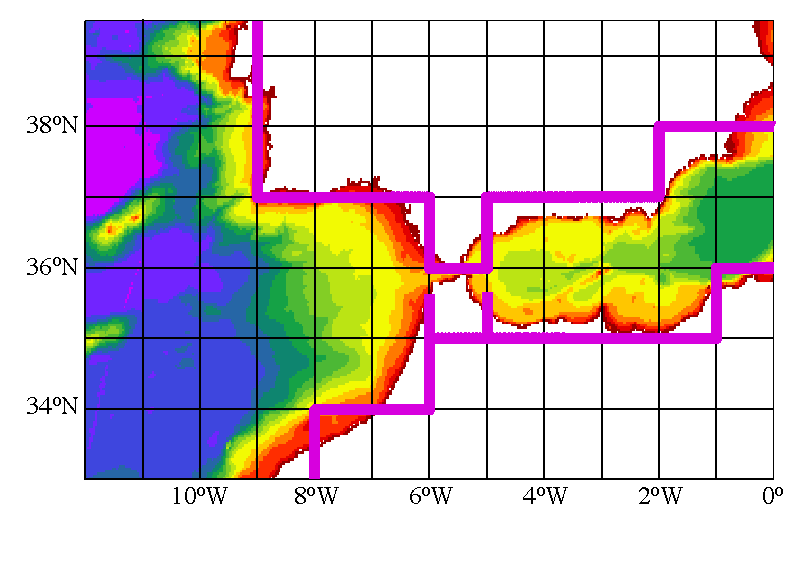
\includegraphics[width=0.80\textwidth]{./TexFiles/Figures/Fig_Gibraltar.pdf}
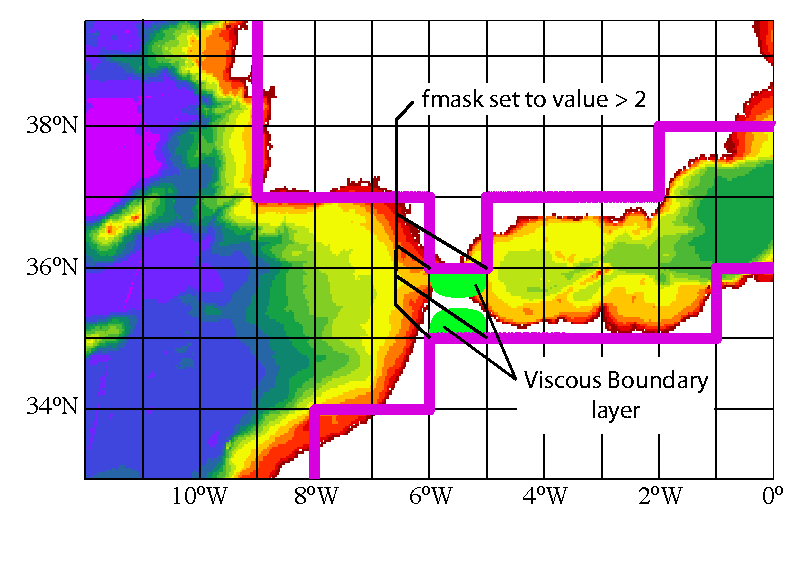
\includegraphics[width=0.80\textwidth]{./TexFiles/Figures/Fig_Gibraltar2.pdf}
\caption{	\label{Fig_MISC_strait_hand} 
Example of the Gibraltar strait defined in a $1\deg \times 1\deg$ mesh. 
\textit{Top}: using partially open cells. The meridional scale factor at $v$-point 
is reduced on both sides of the strait to account for the real width of the strait 
(about 20 km). Note that the scale factors of the strait $T$-point remains unchanged. 
\textit{Bottom}: using viscous boundary layers. The four fmask parameters 
along the strait coastlines are set to a value larger than 4, $i.e.$ "strong" no-slip 
case (see Fig.\ref{Fig_LBC_shlat}) creating a large viscous boundary layer 
that allows a reduced transport through the strait.}
\end{center}   \end{figure}
%>>>>>>>>>>>>>>>>>>>>>>>>>>>>

% -------------------------------------------------------------------------------------------------------------
% Cross Land Advection 
% -------------------------------------------------------------------------------------------------------------
\subsection{Cross Land Advection (\mdl{tracla})}
\label{MISC_strait_cla}
%--------------------------------------------namcla--------------------------------------------------------
\namdisplay{namcla} 
%--------------------------------------------------------------------------------------------------------------

\colorbox{yellow}{Add a short description of CLA staff here or in lateral boundary condition chapter?}
Options are defined through the  \ngn{namcla} namelist variables.

%The problem is resolved here by allowing the mixing of tracers and mass/volume between non-adjacent water columns at nominated regions within the model. Momentum is not mixed. The scheme conserves total tracer content, and total volume (the latter in $z*$- or $s*$-coordinate), and maintains compatibility between the tracer and mass/volume budgets.  

% ================================================================
% Closed seas
% ================================================================
\section{Closed seas (\mdl{closea})}
\label{MISC_closea}

\colorbox{yellow}{Add here a short description of the way closed seas are managed}


% ================================================================
% Sub-Domain Functionality (\textit{nizoom, njzoom}, namelist parameters)
% ================================================================
\section{Sub-Domain Functionality (\np{jpizoom}, \np{jpjzoom})}
\label{MISC_zoom}

The sub-domain functionality, also improperly called the zoom option 
(improperly because it is not associated with a change in model resolution) 
is a quite simple function that allows a simulation over a sub-domain of an 
already defined configuration ($i.e.$ without defining a new mesh, initial 
state and forcings). This option can be useful for testing the user settings 
of surface boundary conditions, or the initial ocean state of a huge ocean 
model configuration while having a small computer memory requirement. 
It can also be used to easily test specific physics in a sub-domain (for example, 
see \citep{Madec_al_JPO96} for a test of the coupling used in the global ocean 
version of OPA between sea-ice and ocean model over the Arctic or Antarctic 
ocean, using a sub-domain). In the standard model, this option does not 
include any specific treatment for the ocean boundaries of the sub-domain: 
they are considered as artificial vertical walls. Nevertheless, it is quite easy 
to add a restoring term toward a climatology in the vicinity of such boundaries 
(see \S\ref{TRA_dmp}).

In order to easily define a sub-domain over which the computation can be 
performed, the dimension of all input arrays (ocean mesh, bathymetry, 
forcing, initial state, ...) are defined as \np{jpidta}, \np{jpjdta} and \np{jpkdta} 
( in \ngn{namcfg} namelist), while the computational domain is defined through 
\np{jpiglo}, \np{jpjglo} and \jp{jpk} (\ngn{namcfg} namelist). When running the 
model over the whole domain, the user sets \np{jpiglo}=\np{jpidta} \np{jpjglo}=\np{jpjdta} 
and \jp{jpk}=\jp{jpkdta}. When running the model over a sub-domain, the user 
has to provide the size of the sub-domain, (\np{jpiglo}, \np{jpjglo}, \np{jpkglo}), 
and the indices of the south western corner as \np{jpizoom} and \np{jpjzoom} in 
the  \ngn{namcfg} namelist (Fig.~\ref{Fig_LBC_zoom}). 

Note that a third set of dimensions exist, \jp{jpi}, \jp{jpj} and \jp{jpk} which is 
actually used to perform the computation. It is set by default to \jp{jpi}=\np{jpjglo} 
and \jp{jpj}=\np{jpjglo}, except for massively parallel computing where the 
computational domain is laid out on local processor memories following a 2D 
horizontal splitting. % (see {\S}IV.2-c) ref to the section to be updated

\subsection{Simple subsetting of input files via netCDF attributes}

The extended grids for use with the under-shelf ice cavities will result in redundant rows
around Antarctica if the ice cavities are not active. A simple mechanism for subsetting
input files associated with the extended domains has been implemented to avoid the need to
maintain different sets of input fields for use with or without active ice cavities. The
existing 'zoom' options are overly complex for this task and marked for deletion anyway.
This alternative subsetting operates for the j-direction only and works by optionally
looking for and using a global file attribute (named: \np{open\_ocean\_jstart}) to
determine the starting j-row for input. The use of this option is best explained with an
example: Consider an ORCA1 configuration using the extended grid bathymetry and coordinate
files:
\vspace{-10pt}
\begin{alltt}
\tiny
\begin{verbatim}
eORCA1_bathymetry_v2.nc
eORCA1_coordinates.nc
\end{verbatim}
\end{alltt}
\noindent These files define a horizontal domain of 362x332. Assuming the first row with
open ocean wet points in the non-isf bathymetry for this set is row 42 (Fortran indexing)
then the formally correct setting for \np{open\_ocean\_jstart} is 41. Using this value as the
first row to be read will result in a 362x292 domain which is the same size as the original
ORCA1 domain. Thus the extended coordinates and bathymetry files can be used with all the
original input files for ORCA1 if the ice cavities are not active (\np{ln\_isfcav =
.false.}). Full instructions for achieving this are:

\noindent Add the new attribute to any input files requiring a j-row offset, i.e:
\vspace{-10pt}
\begin{alltt}
\tiny
\begin{verbatim}
ncatted  -a open_ocean_jstart,global,a,d,41 eORCA1_coordinates.nc 
ncatted  -a open_ocean_jstart,global,a,d,41 eORCA1_bathymetry_v2.nc
\end{verbatim}
\end{alltt}
 
\noindent Add the logical switch to \ngn{namcfg} in the configuration namelist and set true:
%--------------------------------------------namcfg--------------------------------------------------------
\namdisplay{namcfg_orca1}
%--------------------------------------------------------------------------------------------------------------

\noindent Note the j-size of the global domain is the (extended j-size minus
\np{open\_ocean\_jstart} + 1 ) and this must match the size of all datasets other than
bathymetry and coordinates currently. However the option can be extended to any global, 2D
and 3D, netcdf, input field by adding the:
\vspace{-10pt}
\begin{alltt}
\tiny
\begin{verbatim}
lrowattr=ln_use_jattr
\end{verbatim}
\end{alltt}
optional argument to the appropriate \np{iom\_get} call and the \np{open\_ocean\_jstart} attribute to the corresponding input files. It remains the users responsibility to set \np{jpjdta} and \np{jpjglo} values in the \np{namelist\_cfg} file according to their needs.

%>>>>>>>>>>>>>>>>>>>>>>>>>>>>
\begin{figure}[!ht] 	  \begin{center}
\includegraphics[width=0.90\textwidth]{./TexFiles/Figures/Fig_LBC_zoom.pdf}
\caption{	\label{Fig_LBC_zoom}
Position of a model domain compared to the data input domain when the zoom functionality is used.}
\end{center}   \end{figure}
%>>>>>>>>>>>>>>>>>>>>>>>>>>>>


% ================================================================
% Accelerating the Convergence 
% ================================================================
\section{Accelerating the Convergence (\np{nn\_acc} = 1)}
\label{MISC_acc}
%--------------------------------------------namdom-------------------------------------------------------
\namdisplay{namdom} 
%--------------------------------------------------------------------------------------------------------------

Searching an equilibrium state with an global ocean model requires a very long time 
integration period (a few thousand years for a global model). Due to the size of 
the time step required for numerical stability (less than a few hours), 
this usually requires a large elapsed time. In order to overcome this problem, 
\citet{Bryan1984} introduces a technique that is intended to accelerate 
the spin up to equilibrium. It uses a larger time step in 
the tracer evolution equations than in the momentum evolution 
equations. It does not affect the equilibrium solution but modifies the 
trajectory to reach it.

Options are defined through the  \ngn{namdom} namelist variables.
The acceleration of convergence option is used when \np{nn\_acc}=1. In that case, 
$\rdt=rn\_rdt$ is the time step of dynamics while $\widetilde{\rdt}=rdttra$ is the 
tracer time-step. the former is set from the \np{rn\_rdt} namelist parameter while the latter
is computed using a hyperbolic tangent profile and the following namelist parameters : 
\np{rn\_rdtmin}, \np{rn\_rdtmax} and \np{rn\_rdth}. Those three parameters correspond 
to the surface value the deep ocean value and the depth at which the transition occurs, respectively. 
The set of prognostic equations to solve becomes:
\begin{equation} \label{Eq_acc}
\begin{split}
\frac{\partial \textbf{U}_h }{\partial t} 
	&\equiv \frac{\textbf{U}_h ^{t+1}-\textbf{U}_h^{t-1} }{2\rdt} = \ldots \\ 
\frac{\partial T}{\partial t} &\equiv \frac{T^{t+1}-T^{t-1}}{2 \widetilde{\rdt}} = \ldots \\ 
\frac{\partial S}{\partial t} &\equiv \frac{S^{t+1} -S^{t-1}}{2 \widetilde{\rdt}} = \ldots \\ 
\end{split}
\end{equation}

\citet{Bryan1984} has examined the consequences of this distorted physics. 
Free waves have a slower phase speed, their meridional structure is slightly 
modified, and the growth rate of baroclinically unstable waves is reduced 
but with a wider range of instability. This technique is efficient for 
searching for an equilibrium state in coarse resolution models. However its 
application is not suitable for many oceanic problems: it cannot be used for 
transient or time evolving problems (in particular, it is very questionable 
to use this technique when there is a seasonal cycle in the forcing fields), 
and it cannot be used in high-resolution models where baroclinically 
unstable processes are important. Moreover, the vertical variation of 
$\widetilde{ \rdt}$ implies that the heat and salt contents are no longer 
conserved due to the vertical coupling of the ocean level through both 
advection and diffusion. Therefore \np{rn\_rdtmin} = \np{rn\_rdtmax} should be
a more clever choice.


% ================================================================
% Accuracy and Reproducibility
% ================================================================
\section{Accuracy and Reproducibility (\mdl{lib\_fortran})}
\label{MISC_fortran}

\subsection{Issues with intrinsinc SIGN function (\key{nosignedzero})}
\label{MISC_sign}

The SIGN(A, B) is the \textsc {Fortran} intrinsic function delivers the magnitude 
of A with the sign of B. For example, SIGN(-3.0,2.0) has the value 3.0.
The problematic case is when the second argument is zero, because, on platforms 
that support IEEE arithmetic, zero is actually a signed number. 
There is a positive zero and a negative zero.

In \textsc{Fortran}~90, the processor was required always to deliver a positive result for SIGN(A, B) 
if B was zero. Nevertheless, in \textsc{Fortran}~95, the processor is allowed to do the correct thing 
and deliver ABS(A) when B is a positive zero and -ABS(A) when B is a negative zero. 
This change in the specification becomes apparent only when B is of type real, and is zero, 
and the processor is capable of distinguishing between positive and negative zero, 
and B is negative real zero. Then SIGN delivers a negative result where, under \textsc{Fortran}~90 
rules,  it used to return a positive result. 
This change may be especially sensitive for the ice model, so we overwrite the intrinsinc 
function with our own function simply performing :   \\
\verb?   IF( B >= 0.e0 ) THEN   ;   SIGN(A,B) = ABS(A)  ?    \\
\verb?   ELSE                   ;   SIGN(A,B) =-ABS(A)     ?  \\
\verb?   ENDIF    ? \\
This feature can be found in \mdl{lib\_fortran} module and is effective when \key{nosignedzero}
is defined. We use a CPP key as the overwritting of a intrinsic function can present 
performance issues with some computers/compilers.


\subsection{MPP reproducibility}
\label{MISC_glosum}

The numerical reproducibility of simulations on distributed memory parallel computers 
is a critical issue. In particular, within NEMO global summation of distributed arrays 
is most susceptible to rounding errors, and their propagation and accumulation cause 
uncertainty in final simulation reproducibility on different numbers of processors.
To avoid so, based on \citet{He_Ding_JSC01} review of different technics, 
we use a so called self-compensated summation method. The idea is to estimate 
the roundoff error, store it in a buffer, and then add it back in the next addition. 

Suppose we need to calculate $b = a_1 + a_2 + a_3$. The following algorithm 
will allow to split the sum in two ($sum_1 = a_{1} + a_{2}$ and $b = sum_2 = sum_1 + a_3$) 
with exactly the same rounding errors as the sum performed all at once.
\begin{align*}
	sum_1 \ \  &= a_1 + a_2 \\
	error_1     &= a_2 + ( a_1 - sum_1 ) \\
	sum_2 \ \  &= sum_1 + a_3 + error_1 \\
	error_2     &= a_3 + error_1 + ( sum_1 - sum_2 ) \\
	b \qquad \ &= sum_2 \\
\end{align*}
This feature can be found in \mdl{lib\_fortran} module and is effective when \key{mpp\_rep}.
In that case, all calls to glob\_sum function (summation over the entire basin excluding 
duplicated rows and columns due to cyclic or north fold boundary condition as well as 
overlap MPP areas). 
Note this implementation may be sensitive to the optimization level. 

\subsection{MPP scalability}
\label{MISC_mppsca}

The default method of communicating values across the north-fold in distributed memory applications
(\key{mpp\_mpi}) uses a \textsc{MPI\_ALLGATHER} function to exchange values from each processing
region in the northern row with every other processing region in the northern row. This enables a
global width array containing the top 4 rows to be collated on every northern row processor and then
folded with a simple algorithm. Although conceptually simple, this "All to All" communication will
hamper performance scalability for large numbers of northern row processors. From version 3.4
onwards an alternative method is available which only performs direct "Peer to Peer" communications
between each processor and its immediate "neighbours" across the fold line. This is achieved by
using the default \textsc{MPI\_ALLGATHER} method during initialisation to help identify the "active"
neighbours. Stored lists of these neighbours are then used in all subsequent north-fold exchanges to
restrict exchanges to those between associated regions. The collated global width array for each
region is thus only partially filled but is guaranteed to be set at all the locations actually
required by each individual for the fold operation. This alternative method should give identical
results to the default \textsc{ALLGATHER} method and is recommended for large values of \np{jpni}.
The new method is activated by setting \np{ln\_nnogather} to be true ({\bf nammpp}). The
reproducibility of results using the two methods should be confirmed for each new, non-reference
configuration.

% ================================================================
% Model optimisation, Control Print and Benchmark
% ================================================================
\section{Model Optimisation, Control Print and Benchmark}
\label{MISC_opt}
%--------------------------------------------namctl-------------------------------------------------------
\namdisplay{namctl} 
%--------------------------------------------------------------------------------------------------------------

 \gmcomment{why not make these bullets into subsections?}
Options are defined through the  \ngn{namctl} namelist variables.

$\bullet$ Vector optimisation:

\key{vectopt\_loop} enables the internal loops to collapse. This is very 
a very efficient way to increase the length of vector calculations and thus 
to speed up the model on vector computers.
 
% Add here also one word on NPROMA technique that has been found useless, since compiler have made significant progress during the last decade.
 
% Add also one word on NEC specific optimisation (Novercheck option for example)
 
$\bullet$ Control print %: describe here 4 things:

1- \np{ln\_ctl} : compute and print the trends averaged over the interior domain 
in all TRA, DYN, LDF and ZDF modules. This option is very helpful when 
diagnosing the origin of an undesired change in model results. 

2- also \np{ln\_ctl} but using the nictl and njctl namelist parameters to check 
the source of differences between mono and multi processor runs.

3- \key{esopa} (to be rename key\_nemo) : which is another option for model 
management. When defined, this key forces the activation of all options and 
CPP keys. For example, all tracer and momentum advection schemes are called! 
Therefore the model results have no physical meaning. 
However, this option forces both the compiler and the model to run through 
all the \textsc{Fortran} lines of the model. This allows the user to check for obvious 
compilation or execution errors with all CPP options, and errors in namelist options.

4- last digit comparison (\np{nn\_bit\_cmp}). In an MPP simulation, the computation of 
a sum over the whole domain is performed as the summation over all processors of 
each of their sums over their interior domains. This double sum never gives exactly 
the same result as a single sum over the whole domain, due to truncation differences. 
The "bit comparison" option has been introduced in order to be able to check that 
mono-processor and multi-processor runs give exactly the same results. 
%THIS is to be updated with the mpp_sum_glo  introduced in v3.3
% nn_bit_cmp  today only check that the nn_cla = 0 (no cross land advection)

$\bullet$  Benchmark (\np{nn\_bench}). This option defines a benchmark run based on 
a GYRE configuration (see \S\ref{CFG_gyre}) in which the resolution remains the same 
whatever the domain size. This allows a very large model domain to be used, just by 
changing the domain size (\jp{jpiglo}, \jp{jpjglo}) and without adjusting either the time-step 
or the physical parameterisations. 


% ================================================================
% Elliptic solvers (SOL)
% ================================================================
\section{Elliptic solvers (SOL)}
\label{MISC_sol}
%--------------------------------------------namdom-------------------------------------------------------
\namdisplay{namsol} 
%--------------------------------------------------------------------------------------------------------------

When the filtered sea surface height option is used, the surface pressure gradient is 
computed in \mdl{dynspg\_flt}. The force added in the momentum equation is solved implicitely.
It is thus solution of an elliptic equation \eqref{Eq_PE_flt} for which two solvers are available: 
a Successive-Over-Relaxation scheme (SOR) and a preconditioned conjugate gradient 
scheme(PCG) \citep{Madec_al_OM88, Madec_PhD90}. The solver is selected trough the
the value of \np{nn\_solv}   \ngn{namsol} namelist variable. 

The PCG is a very efficient method for solving elliptic equations on vector computers. 
It is a fast and rather easy method to use; which are attractive features for a large 
number of ocean situations (variable bottom topography, complex coastal geometry, 
variable grid spacing, open or cyclic boundaries, etc ...). It does not require 
a search for an optimal parameter as in the SOR method. However, the SOR has 
been retained because it is a linear solver, which is a very useful property when 
using the adjoint model of \NEMO.

At each time step, the time derivative of the sea surface height at time step $t+1$ 
(or equivalently the divergence of the \textit{after} barotropic transport) that appears 
in the filtering forced is the solution of the elliptic equation obtained from the horizontal 
divergence of the vertical summation of \eqref{Eq_PE_flt}. 
Introducing the following coefficients:
\begin{equation}  \label{Eq_sol_matrix}
\begin{aligned}
&c_{i,j}^{NS}  &&= {2 \rdt }^2 \; \frac{H_v (i,j) \; e_{1v} (i,j)}{e_{2v}(i,j)}              \\
&c_{i,j}^{EW} &&= {2 \rdt }^2 \; \frac{H_u (i,j) \; e_{2u} (i,j)}{e_{1u}(i,j)}            \\
&b_{i,j} &&= \delta_i \left[ e_{2u}M_u \right] - \delta_j \left[ e_{1v}M_v \right]\ ,   \\
\end{aligned}
\end{equation}
the resulting five-point finite difference equation is given by:
\begin{equation}  \label{Eq_solmat}
\begin{split}
       c_{i+1,j}^{NS} D_{i+1,j}  + \;  c_{i,j+1}^{EW} D_{i,j+1}   
  +   c_{i,j}    ^{NS} D_{i-1,j}   + \;  c_{i,j}    ^{EW} D_{i,j-1}                                          &    \\
  -    \left(c_{i+1,j}^{NS} + c_{i,j+1}^{EW} + c_{i,j}^{NS} + c_{i,j}^{EW} \right)   D_{i,j}  &=  b_{i,j}
\end{split}
\end{equation}
\eqref{Eq_solmat} is a linear symmetric system of equations. All the elements of 
the corresponding matrix \textbf{A} vanish except those of five diagonals. With 
the natural ordering of the grid points (i.e. from west to east and from 
south to north), the structure of \textbf{A} is block-tridiagonal with 
tridiagonal or diagonal blocks. \textbf{A} is a positive-definite symmetric 
matrix of size $(jpi \cdot jpj)^2$, and \textbf{B}, the right hand side of 
\eqref{Eq_solmat}, is a vector.

Note that in the linear free surface case, the depth that appears in \eqref{Eq_sol_matrix}
does not vary with time, and thus the matrix can be computed once for all. In non-linear free surface 
(\key{vvl} defined) the matrix have to be updated at each time step.

% -------------------------------------------------------------------------------------------------------------
%       Successive Over Relaxation
% -------------------------------------------------------------------------------------------------------------
\subsection{Successive Over Relaxation (\np{nn\_solv}=2, \mdl{solsor})}
\label{MISC_solsor}

Let us introduce the four cardinal coefficients: 
\begin{align*}
a_{i,j}^S &= c_{i,j    }^{NS}/d_{i,j}     &\qquad  a_{i,j}^W &= c_{i,j}^{EW}/d_{i,j}       \\
a_{i,j}^E &= c_{i,j+1}^{EW}/d_{i,j}    &\qquad   a_{i,j}^N &= c_{i+1,j}^{NS}/d_{i,j}   
\end{align*}
where $d_{i,j} = c_{i,j}^{NS}+ c_{i+1,j}^{NS} + c_{i,j}^{EW} + c_{i,j+1}^{EW}$ 
(i.e. the diagonal of the matrix). \eqref{Eq_solmat} can be rewritten as:
\begin{equation}  \label{Eq_solmat_p}
\begin{split}
a_{i,j}^{N}  D_{i+1,j} +\,a_{i,j}^{E}  D_{i,j+1} +\, a_{i,j}^{S}  D_{i-1,j} +\,a_{i,j}^{W} D_{i,j-1}  -  D_{i,j} = \tilde{b}_{i,j}
\end{split}
\end{equation}
with $\tilde b_{i,j} = b_{i,j}/d_{i,j}$. \eqref{Eq_solmat_p} is the equation actually solved 
with the SOR method. This method used is an iterative one. Its algorithm can be 
summarised as follows (see \citet{Haltiner1980} for a further discussion):

initialisation (evaluate a first guess from previous time step computations)
\begin{equation}
D_{i,j}^0 = 2 \, D_{i,j}^t - D_{i,j}^{t-1}
\end{equation}
iteration $n$, from $n=0$ until convergence, do :
\begin{equation} \label{Eq_sor_algo}
\begin{split}
R_{i,j}^n  = &a_{i,j}^{N} D_{i+1,j}^n       +\,a_{i,j}^{E}  D_{i,j+1} ^n	    	
			+\, a_{i,j}^{S}  D_{i-1,j} ^{n+1}+\,a_{i,j}^{W} D_{i,j-1} ^{n+1}
                 -  D_{i,j}^n - \tilde{b}_{i,j}                                           \\
D_{i,j} ^{n+1}  = &D_{i,j} ^{n}   + \omega \;R_{i,j}^n     
\end{split}
\end{equation}
where \textit{$\omega $ }satisfies $1\leq \omega \leq 2$. An optimal value exists for 
\textit{$\omega$} which significantly accelerates the convergence, but it has to be 
adjusted empirically for each model domain (except for a uniform grid where an 
analytical expression for \textit{$\omega$} can be found \citep{Richtmyer1967}). 
The value of $\omega$ is set using \np{rn\_sor}, a \textbf{namelist} parameter. 
The convergence test is of the form:
\begin{equation}
\delta = \frac{\sum\limits_{i,j}{R_{i,j}^n}{R_{i,j}^n}}
                    {\sum\limits_{i,j}{ \tilde{b}_{i,j}^n}{\tilde{b}_{i,j}^n}} \leq \epsilon
\end{equation}
where $\epsilon$ is the absolute precision that is required. It is recommended 
that a value smaller or equal to $10^{-6}$ is used for $\epsilon$ since larger 
values may lead to numerically induced basin scale barotropic oscillations. 
The precision is specified by setting \np{rn\_eps} (\textbf{namelist} parameter). 
In addition, two other tests are used to halt the iterative algorithm. They involve 
the number of iterations and the modulus of the right hand side. If the former 
exceeds a specified value, \np{nn\_max} (\textbf{namelist} parameter), 
or the latter is greater than $10^{15}$, the whole model computation is stopped 
and the last computed time step fields are saved in a abort.nc NetCDF file. 
In both cases, this usually indicates that there is something wrong in the model 
configuration (an error in the mesh, the initial state, the input forcing, 
or the magnitude of the time step or of the mixing coefficients). A typical value of 
$nn\_max$ is a few hundred when $\epsilon = 10^{-6}$, increasing to a few 
thousand when $\epsilon = 10^{-12}$.
The vectorization of the SOR algorithm is not straightforward. The scheme
contains two linear recurrences on $i$ and $j$. This inhibits the vectorisation. 
\eqref{Eq_sor_algo} can be been rewritten as:
\begin{equation} 
\begin{split}
R_{i,j}^n
= &a_{i,j}^{N}  D_{i+1,j}^n +\,a_{i,j}^{E}  D_{i,j+1} ^n
 +\,a_{i,j}^{S}  D_{i-1,j} ^{n}+\,_{i,j}^{W} D_{i,j-1} ^{n} -  D_{i,j}^n - \tilde{b}_{i,j}      \\
R_{i,j}^n = &R_{i,j}^n - \omega \;a_{i,j}^{S}\; R_{i,j-1}^n                                             \\
R_{i,j}^n = &R_{i,j}^n - \omega \;a_{i,j}^{W}\; R_{i-1,j}^n
\end{split}
\end{equation}
This technique slightly increases the number of iteration required to reach the convergence,
but this is largely compensated by the gain obtained by the suppression of the recurrences.

Another technique have been chosen, the so-called red-black SOR. It consist in solving successively 
\eqref{Eq_sor_algo} for odd and even grid points. It also slightly reduced the convergence rate
but allows the vectorisation. In addition, and this is the reason why it has been chosen, it is able to handle the north fold boundary condition used in ORCA configuration ($i.e.$ tri-polar global ocean mesh).

The SOR method is very flexible and can be used under a wide range of conditions, 
including irregular boundaries, interior boundary points, etc. Proofs of convergence, etc. 
may be found in the standard numerical methods texts for partial differential equations.

% -------------------------------------------------------------------------------------------------------------
%       Preconditioned Conjugate Gradient
% -------------------------------------------------------------------------------------------------------------
\subsection{Preconditioned Conjugate Gradient  (\np{nn\_solv}=1, \mdl{solpcg}) }
\label{MISC_solpcg}

\textbf{A} is a definite positive symmetric matrix, thus solving the linear 
system \eqref{Eq_solmat} is equivalent to the minimisation of a quadratic 
functional:
\begin{equation*}
\textbf{Ax} = \textbf{b} \leftrightarrow \textbf{x} =\text{inf}_{y} \,\phi (\textbf{y})
\quad , \qquad
\phi (\textbf{y}) = 1/2 \langle \textbf{Ay},\textbf{y}\rangle - \langle \textbf{b},\textbf{y} \rangle 
\end{equation*}
where $\langle , \rangle$ is the canonical dot product. The idea of the 
conjugate gradient method is to search for the solution in the following 
iterative way: assuming that $\textbf{x}^n$ has been obtained, $\textbf{x}^{n+1}$ 
is found from $\textbf {x}^{n+1}={\textbf {x}}^n+\alpha^n{\textbf {d}}^n$ which satisfies:
\begin{equation*}
{\textbf{ x}}^{n+1}=\text{inf} _{{\textbf{ y}}={\textbf{ x}}^n+\alpha^n \,{\textbf{ d}}^n} \,\phi ({\textbf{ y}})\;\;\Leftrightarrow \;\;\frac{d\phi }{d\alpha}=0
\end{equation*}
and expressing $\phi (\textbf{y})$ as a function of \textit{$\alpha $}, we obtain the 
value that minimises the functional: 
\begin{equation*}
\alpha ^n = \langle{ \textbf{r}^n , \textbf{r}^n} \rangle  / \langle {\textbf{ A d}^n, \textbf{d}^n} \rangle
\end{equation*}
where $\textbf{r}^n = \textbf{b}-\textbf{A x}^n = \textbf{A} (\textbf{x}-\textbf{x}^n)$ 
is the error at rank $n$. The descent vector $\textbf{d}^n$ s chosen to be dependent 
on the error: $\textbf{d}^n = \textbf{r}^n + \beta^n \,\textbf{d}^{n-1}$. $\beta ^n$ 
is searched such that the descent vectors form an orthogonal basis for the dot 
product linked to \textbf{A}. Expressing the condition 
$\langle \textbf{A d}^n, \textbf{d}^{n-1} \rangle = 0$ the value of $\beta ^n$ is found:
 $\beta ^n = \langle{ \textbf{r}^n , \textbf{r}^n} \rangle  / \langle {\textbf{r}^{n-1}, \textbf{r}^{n-1}} \rangle$. 
 As a result, the errors $ \textbf{r}^n$ form an orthogonal 
base for the canonic dot product while the descent vectors $\textbf{d}^n$ form 
an orthogonal base for the dot product linked to \textbf{A}. The resulting 
algorithm is thus the following one:

initialisation :
\begin{equation*} 
\begin{split}
\textbf{x}^0 &= D_{i,j}^0   = 2 D_{i,j}^t - D_{i,j}^{t-1}       \quad, \text{the initial guess }     \\
\textbf{r}^0 &= \textbf{d}^0 = \textbf{b} - \textbf{A x}^0       \\
\gamma_0 &= \langle{ \textbf{r}^0 , \textbf{r}^0} \rangle
\end{split}
\end{equation*}

iteration $n,$ from $n=0$ until convergence, do :
\begin{equation} 
\begin{split}
\text{z}^n& = \textbf{A d}^n \\
\alpha_n &= \gamma_n /  \langle{ \textbf{z}^n , \textbf{d}^n} \rangle \\
\textbf{x}^{n+1} &= \textbf{x}^n + \alpha_n \,\textbf{d}^n \\
\textbf{r}^{n+1} &= \textbf{r}^n - \alpha_n \,\textbf{z}^n \\
\gamma_{n+1} &= \langle{ \textbf{r}^{n+1} , \textbf{r}^{n+1}} \rangle \\
\beta_{n+1} &= \gamma_{n+1}/\gamma_{n}  \\
\textbf{d}^{n+1} &= \textbf{r}^{n+1} + \beta_{n+1}\; \textbf{d}^{n}\\
\end{split}
\end{equation}


The convergence test is:
\begin{equation}
\delta = \gamma_{n}\; / \langle{ \textbf{b} , \textbf{b}} \rangle \leq \epsilon
\end{equation}
where $\epsilon $ is the absolute precision that is required. As for the SOR algorithm, 
the whole model computation is stopped when the number of iterations, \np{nn\_max}, or 
the modulus of the right hand side of the convergence equation exceeds a 
specified value (see \S\ref{MISC_solsor} for a further discussion). The required 
precision and the maximum number of iterations allowed are specified by setting 
\np{rn\_eps} and \np{nn\_max} (\textbf{namelist} parameters).

It can be demonstrated that the above algorithm is optimal, provides the exact 
solution in a number of iterations equal to the size of the matrix, and that 
the convergence rate is faster as the matrix is closer to the identity matrix,
$i.e.$ its eigenvalues are closer to 1. Therefore, it is more efficient to solve 
a better conditioned system which has the same solution. For that purpose, 
we introduce a preconditioning matrix \textbf{Q} which is an approximation 
of \textbf{A} but much easier to invert than \textbf{A}, and solve the system:
\begin{equation} \label{Eq_pmat}
\textbf{Q}^{-1} \textbf{A x} = \textbf{Q}^{-1} \textbf{b}
\end{equation}

The same algorithm can be used to solve \eqref{Eq_pmat} if instead of the 
canonical dot product the following one is used: 
${\langle{ \textbf{a} , \textbf{b}} \rangle}_Q = \langle{ \textbf{a} , \textbf{Q b}} \rangle$, and 
if $\textbf{\~{b}} = \textbf{Q}^{-1}\;\textbf{b}$ and $\textbf{\~{A}} = \textbf{Q}^{-1}\;\textbf{A}$ 
are substituted to \textbf{b} and \textbf{A} \citep{Madec_al_OM88}. 
In \NEMO, \textbf{Q} is chosen as the diagonal of \textbf{ A}, i.e. the simplest form for 
\textbf{Q} so that it can be easily inverted. In this case, the discrete formulation of 
\eqref{Eq_pmat} is in fact given by \eqref{Eq_solmat_p} and thus the matrix and 
right hand side are computed independently from the solver used.

% ================================================================












			% Miscellaneous topics

% ================================================================
% Chapter � Configurations
% ================================================================
\chapter{Configurations}
\label{CFG}
\minitoc

\newpage
$\ $\newline    % force a new ligne

% ================================================================
% Introduction
% ================================================================
\section{Introduction}
\label{CFG_intro}


The purpose of this part of the manual is to introduce the \NEMO reference configurations. 
These configurations are offered as means to explore various numerical and physical options, 
thus allowing the user to verify that the code is performing in a manner consistent with that 
we are running. This form of verification is critical as one adopts the code for his or her particular 
research purposes. The test cases also provide a sense for some of the options available 
in the code, though by no means are all options exercised in the reference configurations.

Configuration is defined mainly through the \ngn{namcfg} namelist variables:
%------------------------------------------namcfg----------------------------------------------------
\namdisplay{namcfg}
%-------------------------------------------------------------------------------------------------------------

% ================================================================
% 1D model configuration
% ================================================================
\section{Water column model: 1D model (C1D) (\key{c1d}) }
\label{CFG_c1d}

The 1D model option simulates a stand alone water column within the 3D \NEMO system. 
It can be applied to the ocean alone or to the ocean-ice system and can include passive tracers 
or a biogeochemical model. It is set up by defining the position of the 1D water column in the grid 
(see \textit{CONFIG/SHARED/namelist\_ref} ). 
The 1D model is a very useful tool  
\textit{(a)} to learn about the physics and numerical treatment of vertical mixing processes ; 
\textit{(b)} to investigate suitable parameterisations of unresolved turbulence (surface wave
breaking, Langmuir circulation, ...) ; 
\textit{(c)} to compare the behaviour of different vertical mixing schemes  ; 
\textit{(d)} to perform sensitivity studies on the vertical diffusion at a particular point of an ocean domain ; 
\textit{(d)} to produce extra diagnostics, without the large memory requirement of the full 3D model.

The methodology is based on the use of the zoom functionality over the smallest possible 
domain : a 3x3 domain centered on the grid point of interest, 
with some extra routines. There is no need to define a new mesh, bathymetry, 
initial state or forcing, since the 1D model will use those of the configuration it is a zoom of. 
The chosen grid point is set in \textit{\ngn{namcfg}} namelist by setting the \np{jpizoom} and \np{jpjzoom} 
parameters to the indices of the location of the chosen grid point.

The 1D model has some specifies. First, all the horizontal derivatives are assumed to be zero, and
second, the two components of the velocity are moved on a $T$-point. 
Therefore, defining \key{c1d} changes five main things in the code behaviour: 
\begin{description}
\item[(1)] the lateral boundary condition routine (\rou{lbc\_lnk}) set the value of the central column 
of the 3x3 domain is imposed over the whole domain ; 
\item[(3)] a call to \rou{lbc\_lnk} is systematically done when reading input data ($i.e.$ in \mdl{iom}) ; 
\item[(3)] a simplified \rou{stp} routine is used (\rou{stp\_c1d}, see \mdl{step\_c1d} module) in which 
both lateral tendancy terms and lateral physics are not called ; 
\item[(4)] the vertical velocity is zero (so far, no attempt at introducing a Ekman pumping velocity 
has been made) ; 
\item[(5)] a simplified treatment of the Coriolis term is performed as $U$- and $V$-points are the same 
(see \mdl{dyncor\_c1d}).
\end{description}
All the relevant \textit{\_c1d} modules can be found in the NEMOGCM/NEMO/OPA\_SRC/C1D directory of 
the \NEMO distribution.

% to be added:  a test case on the yearlong Ocean Weather Station (OWS) Papa dataset of Martin (1985)

% ================================================================
% ORCA family configurations
% ================================================================
\section{ORCA family: global ocean with tripolar grid }
\label{CFG_orca}

The ORCA family is a series of global ocean configurations that are run together with 
the LIM sea-ice model (ORCA-LIM) and possibly with PISCES biogeochemical model 
(ORCA-LIM-PISCES), using various resolutions.
The appropriate \textit{\&namcfg} namelist is available in \textit{CONFIG/ORCA2\_LIM/EXP00/namelist\_cfg} 
for ORCA2 and in \textit{CONFIG/SHARED/README\_other\_configurations\_namelist\_namcfg} 
for other resolutions


%>>>>>>>>>>>>>>>>>>>>>>>>>>>>
\begin{figure}[!t]   \begin{center}
\includegraphics[width=0.98\textwidth]{./TexFiles/Figures/Fig_ORCA_NH_mesh.pdf}
\caption{  \label{Fig_MISC_ORCA_msh}     
ORCA mesh conception. The departure from an isotropic Mercator grid start poleward of 20\deg N.
The two "north pole" are the foci of a series of embedded ellipses (blue curves) 
which are determined analytically and form the i-lines of the ORCA mesh (pseudo latitudes). 
Then, following \citet{Madec_Imbard_CD96}, the normal to the series of ellipses (red curves) is computed 
which provide the j-lines of the mesh (pseudo longitudes).  }
\end{center}   \end{figure}
%>>>>>>>>>>>>>>>>>>>>>>>>>>>>

% -------------------------------------------------------------------------------------------------------------
%       ORCA tripolar grid
% -------------------------------------------------------------------------------------------------------------
\subsection{ORCA tripolar grid}
\label{CFG_orca_grid}

The ORCA grid is a tripolar is based on the semi-analytical method of \citet{Madec_Imbard_CD96}. 
It allows to construct a global orthogonal curvilinear ocean mesh which has no singularity point inside 
the computational domain since two north mesh poles are introduced and placed on lands.
The method involves defining an analytical set of mesh parallels in the stereographic polar plan, 
computing the associated set of mesh meridians, and projecting the resulting mesh onto the sphere. 
The set of mesh parallels used is a series of embedded ellipses which foci are the two mesh north 
poles (Fig.~\ref{Fig_MISC_ORCA_msh}). The resulting mesh presents no loss of continuity in 
either the mesh lines or the scale factors, or even the scale factor derivatives over the whole 
ocean domain, as the mesh is not a composite mesh. 
%>>>>>>>>>>>>>>>>>>>>>>>>>>>>
\begin{figure}[!tbp]  \begin{center}
\includegraphics[width=1.0\textwidth]{./TexFiles/Figures/Fig_ORCA_NH_msh05_e1_e2.pdf}
\includegraphics[width=0.80\textwidth]{./TexFiles/Figures/Fig_ORCA_aniso.pdf}
\caption {  \label{Fig_MISC_ORCA_e1e2}
\textit{Top}: Horizontal scale factors ($e_1$, $e_2$) and 
\textit{Bottom}: ratio of anisotropy ($e_1 / e_2$)
for ORCA 0.5\deg ~mesh. South of 20\deg N a Mercator grid is used ($e_1 = e_2$) 
so that the anisotropy ratio is 1. Poleward of 20\deg N, the two "north pole" 
introduce a weak anisotropy over the ocean areas ($< 1.2$) except in vicinity of Victoria Island 
(Canadian Arctic Archipelago). }
\end{center}   \end{figure}
%>>>>>>>>>>>>>>>>>>>>>>>>>>>>


The method is applied to Mercator grid ($i.e.$ same zonal and meridional grid spacing) poleward 
of $20\deg$N, so that the Equator is a mesh line, which provides a better numerical solution 
for equatorial dynamics. The choice of the series of embedded ellipses (position of the foci and 
variation of the ellipses) is a compromise between maintaining  the ratio of mesh anisotropy 
($e_1 / e_2$) close to one in the ocean (especially in area of strong eddy activities such as 
the Gulf Stream) and keeping the smallest scale factor in the northern hemisphere larger 
than the smallest one in the southern hemisphere.
The resulting mesh is shown in Fig.~\ref{Fig_MISC_ORCA_msh} and \ref{Fig_MISC_ORCA_e1e2} 
for a half a degree grid (ORCA\_R05). The smallest ocean scale factor is found in along  
Antarctica, while the ratio of anisotropy remains close to one except near the Victoria Island 
in the Canadian Archipelago. 

% -------------------------------------------------------------------------------------------------------------
%       ORCA-LIM(-PISCES) configurations
% -------------------------------------------------------------------------------------------------------------
\subsection{ORCA pre-defined resolution}
\label{CFG_orca_resolution}


The NEMO system is provided with five built-in ORCA configurations which differ in the 
horizontal resolution. The value of the resolution is given by the resolution at the Equator 
expressed in degrees. Each of configuration is set through the \textit{\ngn{namcfg}} namelist, 
which sets the grid size and configuration 
name parameters  (Tab. \ref{Tab_ORCA}).
.

%--------------------------------------------------TABLE--------------------------------------------------
\begin{table}[!t]     \begin{center}
\begin{tabular}{p{4cm} c c c c}
Horizontal Grid         	             & \np{jp\_cfg} &  \np{jpiglo} & \np{jpjglo} &       \\  
\hline  \hline
\~4\deg	   &        4         &         92     &      76      &       \\
\~2\deg        &        2         &       182     &    149      &        \\
\~1\deg        &        1         &       362     &     292     &        \\
\~0.5\deg     &        05       &       722     &     511     &        \\
\~0.25\deg   &        025     &      1442    &   1021     &        \\
%\key{orca\_r8}       &        8         &      2882    &   2042     &        \\
%\key{orca\_r12}     &      12         &      4322    &   3062      &       \\
\hline   \hline
\end{tabular}
\caption{ \label{Tab_ORCA}   
Set of predefined parameters for ORCA family configurations.
In all cases, the name of the configuration is set to "orca" ($i.e.$ \np{cp\_cfg}~=~orca). }
\end{center}
\end{table}
%--------------------------------------------------------------------------------------------------------------


The ORCA\_R2 configuration has the following specificity : starting from a 2\deg~ORCA mesh, 
local mesh refinements were applied to the Mediterranean, Red, Black and Caspian Seas, 
so that the resolution is $1\deg \time 1\deg$ there. A local transformation were also applied 
with in the Tropics in order to refine the meridional resolution up to 0.5\deg at the Equator.

The ORCA\_R1 configuration has only a local tropical transformation  to refine the meridional 
resolution up to 1/3\deg~at the Equator. Note that the tropical mesh refinements in ORCA\_R2 
and R1 strongly increases the mesh anisotropy there.

The ORCA\_R05 and higher global configurations do not incorporate any regional refinements.  

For ORCA\_R1 and R025, setting the configuration key to 75 allows to use 75 vertical levels, 
otherwise 46 are used. In the other ORCA configurations, 31 levels are used 
(see Tab.~\ref{Tab_orca_zgr} and Fig.~\ref{Fig_zgr}).

Only the ORCA\_R2 is provided with all its input files in the \NEMO distribution. 
It is very similar to that used as part of the climate model developed at IPSL for the 4th IPCC 
assessment of climate change (Marti et al., 2009). It is also the basis for the \NEMO contribution 
to the Coordinate Ocean-ice Reference Experiments (COREs) documented in \citet{Griffies_al_OM09}. 

This version of ORCA\_R2 has 31 levels in the vertical, with the highest resolution (10m) 
in the upper 150m (see Tab.~\ref{Tab_orca_zgr} and Fig.~\ref{Fig_zgr}). 
The bottom topography and the coastlines are derived from the global atlas of Smith and Sandwell (1997). 
The default forcing uses the boundary forcing from \citet{Large_Yeager_Rep04} (see \S\ref{SBC_blk_core}), 
which was developed for the purpose of running global coupled ocean-ice simulations 
without an interactive atmosphere. This \citet{Large_Yeager_Rep04} dataset is available 
through the \href{http://nomads.gfdl.noaa.gov/nomads/forms/mom4/CORE.html}{GFDL web site}. 
The "normal year" of \citet{Large_Yeager_Rep04} has been chosen of the \NEMO distribution 
since release v3.3. 

ORCA\_R2 pre-defined configuration can also be run with an AGRIF zoom over the Agulhas 
current area ( \key{agrif}  defined) and,  by setting the appropriate variables in 
\textit{\&namcfg}, see \textit{CONFIG/SHARED/namelist\_ref}
a regional Arctic or peri-Antarctic configuration is extracted from an ORCA\_R2 or R05 configurations
using sponge layers at open boundaries. 

% -------------------------------------------------------------------------------------------------------------
%       GYRE family: double gyre basin
% -------------------------------------------------------------------------------------------------------------
\section{GYRE family: double gyre basin }
\label{CFG_gyre}

The GYRE configuration \citep{Levy_al_OM10} has been built to simulate
the seasonal cycle of a double-gyre box model. It consists in an idealized domain 
similar to that used in the studies of \citet{Drijfhout_JPO94} and \citet{Hazeleger_Drijfhout_JPO98, 
Hazeleger_Drijfhout_JPO99, Hazeleger_Drijfhout_JGR00, Hazeleger_Drijfhout_JPO00}, 
over which an analytical seasonal forcing is applied. This allows to investigate the 
spontaneous generation of a large number of interacting, transient mesoscale eddies 
and their contribution to the large scale circulation. 

The domain geometry is a closed rectangular basin on the $\beta$-plane centred 
at $\sim 30\deg$N and rotated by 45\deg, 3180~km long, 2120~km wide 
and 4~km deep (Fig.~\ref{Fig_MISC_strait_hand}). 
The domain is bounded by vertical walls and by a flat bottom. The configuration is 
meant to represent an idealized North Atlantic or North Pacific basin. 
The circulation is forced by analytical profiles of wind and buoyancy fluxes. 
The applied forcings vary seasonally in a sinusoidal manner between winter 
and summer extrema \citep{Levy_al_OM10}. 
The wind stress is zonal and its curl changes sign at 22\deg N and 36\deg N. 
It forces a subpolar gyre in the north, a subtropical gyre in the wider part of the domain 
and a small recirculation gyre in the southern corner. 
The net heat flux takes the form of a restoring toward a zonal apparent air 
temperature profile. A portion of the net heat flux which comes from the solar radiation
is allowed to penetrate within the water column. 
The fresh water flux is also prescribed and varies zonally. 
It is determined such as, at each time step, the basin-integrated flux is zero. 
The basin is initialised at rest with vertical profiles of temperature and salinity 
uniformly applied to the whole domain.

The GYRE configuration is set through the \textit{\&namcfg} namelist defined in the reference 
configuration \textit{CONFIG/GYRE/EXP00/namelist\_cfg}. Its horizontal resolution 
(and thus the size of the domain) is determined by setting \np{jp\_cfg} : \\
\np{jpiglo} $= 30 \times$ \np{jp\_cfg} + 2   \\
\np{jpjglo} $= 20 \times$ \np{jp\_cfg} + 2   \\
Obviously, the namelist parameters have to be adjusted to the chosen resolution, see the Configurations 
pages on the NEMO web site (Using NEMO\/Configurations) .
In the vertical, GYRE uses the default 30 ocean levels (\pp{jpk}=31) (Fig.~\ref{Fig_zgr}).

The GYRE configuration is also used in benchmark test as it is very simple to increase 
its resolution and as it does not requires any input file. For example, keeping a same model size 
on each processor while increasing the number of processor used is very easy, even though the 
physical integrity of the solution can be compromised.

%>>>>>>>>>>>>>>>>>>>>>>>>>>>>
\begin{figure}[!t]   \begin{center}
\includegraphics[width=1.0\textwidth]{./TexFiles/Figures/Fig_GYRE.pdf}
\caption{  \label{Fig_GYRE}   
Snapshot of relative vorticity at the surface of the model domain 
in GYRE R9, R27 and R54. From \citet{Levy_al_OM10}.}
\end{center}   \end{figure}
%>>>>>>>>>>>>>>>>>>>>>>>>>>>>

% -------------------------------------------------------------------------------------------------------------
%       EEL family configuration
% -------------------------------------------------------------------------------------------------------------
\section{EEL family: periodic channel}
\label{MISC_config_EEL}

\begin{description}
\item[eel\_r2]  to be described....
\item[eel\_r5]  
\item[eel\_r6]  
\end{description}
The appropriate \textit{\&namcfg} namelists are available in  
\textit{CONFIG/SHARED/README\_other\_configurations\_namelist\_namcfg}
% -------------------------------------------------------------------------------------------------------------
%       AMM configuration
% -------------------------------------------------------------------------------------------------------------
\section{AMM: atlantic margin configuration }
\label{MISC_config_AMM}

The AMM, Atlantic Margins Model, is a regional model covering the
Northwest European Shelf domain on a regular lat-lon grid at
approximately 12km horizontal resolution. The appropriate 
\textit{\&namcfg} namelist  is available in \textit{CONFIG/AMM12/EXP00/namelist\_cfg}.
It is used to build the correct dimensions of the AMM domain.

This configuration tests several features of NEMO functionality specific
to the shelf seas.
In particular, the AMM uses $S$-coordinates in the vertical rather than
$z$-coordinates and is forced with tidal lateral boundary conditions
using a flather boundary condition from the BDY module (key\_bdy).
The AMM configuration  uses the GLS (key\_zdfgls) turbulence scheme, the
VVL non-linear free surface(key\_vvl) and time-splitting
(key\_dynspg\_ts).

In addition to the tidal boundary condition the model may also take
open boundary conditions from a North Atlantic model. Boundaries may be
completely ommited by removing the BDY key (key\_bdy).
Sample surface fluxes, river forcing and a sample initial restart file
are included to test a realistic model run. The Baltic boundary is
included within the river input file and is specified as a river source.
Unlike ordinary river points the Baltic inputs also include salinity and
temperature data.

			% Predefined configurations

% ================================================================
% APPENDIX
% ================================================================

\appendix

%
% ================================================================
% Invariant of the Equations
% ================================================================
\chapter{Invariants of the Primitive Equations}
\label{Invariant}
\minitoc

The continuous equations of motion have many analytic properties. Many 
quantities (total mass, energy, enstrophy, etc.) are strictly conserved in 
the inviscid and unforced limit, while ocean physics conserve the total 
quantities on which they act (momentum, temperature, salinity) but dissipate 
their total variance (energy, enstrophy, etc.). Unfortunately, the finite 
difference form of these equations is not guaranteed to retain all these 
important properties. In constructing the finite differencing schemes, we 
wish to ensure that certain integral constraints will be maintained. In 
particular, it is desirable to construct the finite difference equations so 
that horizontal kinetic energy and/or potential enstrophy of horizontally 
non-divergent flow, and variance of temperature and salinity will be 
conserved in the absence of dissipative effects and forcing. \citet{Arakawa1966} 
has first pointed out the advantage of this approach. He showed that if 
integral constraints on energy are maintained, the computation will be free 
of the troublesome "non linear" instability originally pointed out by 
\citet{Phillips1959}. A consistent formulation of the energetic properties is 
also extremely important in carrying out long-term numerical simulations for 
an oceanographic model. Such a formulation avoids systematic errors that 
accumulate with time \citep{Bryan1997}.

The general philosophy of OPA which has led to the discrete formulation 
presented in {\S}II.2 and II.3 is to choose second order non-diffusive 
scheme for advective terms for both dynamical and tracer equations. At this 
level of complexity, the resulting schemes are dispersive schemes. 
Therefore, they require the addition of a diffusive operator to be stable. 
The alternative is to use diffusive schemes such as upstream or flux 
corrected schemes. This last option was rejected because we prefer a 
complete handling of the model diffusion, i.e. of the model physics rather 
than letting the advective scheme produces its own implicit diffusion 
without controlling the space and time structure of this implicit diffusion. 
Note that in some very specific cases as passive tracer studies, the 
positivity of the advective scheme is required. In that case, and in that 
case only, the advective scheme used for passive tracer is a flux correction 
scheme \citep{Marti1992, Levy1996, Levy1998}.

% -------------------------------------------------------------------------------------------------------------
%       Conservation Properties on Ocean Dynamics
% -------------------------------------------------------------------------------------------------------------
\section{Conservation Properties on Ocean Dynamics}
\label{Invariant_dyn}

The non linear term of the momentum equations has been split into a 
vorticity term, a gradient of horizontal kinetic energy and a vertical 
advection term. Three schemes are available for the former (see {\S}~II.2) 
according to the CPP variable defined (default option\textbf{ 
}or \textbf{key{\_}vorenergy } or \textbf{key{\_}vorcombined 
} defined). They differ in their conservative 
properties (energy or enstrophy conserving scheme). The two latter terms 
preserve the total kinetic energy: the large scale kinetic energy is also 
preserved in practice. The remaining non-diffusive terms of the momentum 
equation (namely the hydrostatic and surface pressure gradient terms) also 
preserve the total kinetic energy and have no effect on the vorticity of the 
flow.

\textbf{* relative, planetary and total vorticity term:}

Let us define as either the relative, planetary and total potential 
vorticity, i.e. , , and , respectively. The continuous formulation of the 
vorticity term satisfies following integral constraints:
\begin{equation} \label{Eq_vor_vorticity}
\int_D {{\textbf {k}}\cdot \frac{1}{e_3 }\nabla \times \left( {\varsigma 
\;{\rm {\bf k}}\times {\textbf {U}}_h } \right)\;dv} =0
\end{equation}

\begin{equation} \label{Eq_vor_enstrophy}
if\quad \chi =0\quad \quad \int\limits_D {\varsigma \;{\textbf{k}}\cdot 
\frac{1}{e_3 }\nabla \times \left( {\varsigma {\textbf{k}}\times {\textbf{U}}_h } \right)\;dv} =-\int\limits_D {\frac{1}{2}\varsigma ^2\,\chi \;dv} 
=0
\end{equation}

\begin{equation} \label{Eq_vor_energy}
\int_D {{\textbf{U}}_h \times \left( {\varsigma \;{\textbf{k}}\times {\textbf{U}}_h } \right)\;dv} =0
\end{equation}
where $dv = e_1\, e_2\, e_3\, di\, dj\, dk$ is the volume element. 
(II.4.1a) means that $\varsigma $ is conserved. (II.4.1b) is obtained by an 
integration by part. It means that $\varsigma^2$ is conserved for a horizontally 
non-divergent flow. 
(II.4.1c) is even satisfied locally since the vorticity term is orthogonal 
to the horizontal velocity. It means that the vorticity term has no 
contribution to the evolution of the total kinetic energy. (II.4.1a) is 
obviously always satisfied, but (II.4.1b) and (II.4.1c) cannot be satisfied 
simultaneously with a second order scheme. Using the symmetry or 
anti-symmetry properties of the operators (Eqs II.1.10 and 11), it can be 
shown that the scheme (II.2.11) satisfies (II.4.1b) but not (II.4.1c), while 
scheme (II.2.12) satisfies (II.4.1c) but not (II.4.1b) (see appendix C). 
Note that the enstrophy conserving scheme on total vorticity has been chosen 
as the standard discrete form of the vorticity term.

\textbf{* Gradient of kinetic energy / vertical advection}

In continuous formulation, the gradient of horizontal kinetic energy has no 
contribution to the evolution of the vorticity as the curl of a gradient is 
zero. This property is satisfied locally with the discrete form of both the 
gradient and the curl operator we have made (property (II.1.9)~). Another 
continuous property is that the change of horizontal kinetic energy due to 
vertical advection is exactly balanced by the change of horizontal kinetic 
energy due to the horizontal gradient of horizontal kinetic energy:

\begin{equation} \label{Eq_keg_zad}
\int_D {{\textbf{U}}_h \cdot \nabla _h \left( {1/2\;{\textbf{U}}_h ^2} \right)\;dv} =-\int_D {{\textbf{U}}_h \cdot \frac{w}{e_3 }\;\frac{\partial 
{\textbf{U}}_h }{\partial k}\;dv}
\end{equation}

Using the discrete form given in {\S}II.2-a and the symmetry or 
anti-symmetry properties of the mean and difference operators, \eqref{Eq_keg_zad} is 
demonstrated in the Appendix C. The main point here is that satisfying 
\eqref{Eq_keg_zad} links the choice of the discrete forms of the vertical advection 
and of the horizontal gradient of horizontal kinetic energy. Choosing one 
imposes the other. The discrete form of the vertical advection given in 
{\S}II.2-a is a direct consequence of formulating the horizontal kinetic 
energy as $1/2 \left( \overline{u^2}^i + \overline{v^2}^j \right) $ in the gradient term.

\textbf{* hydrostatic pressure gradient term}

In continuous formulation, a pressure gradient has no contribution to the 
evolution of the vorticity as the curl of a gradient is zero. This 
properties is satisfied locally with the choice of discretization we have 
made (property (II.1.9)~). In addition, when the equation of state is linear 
(i.e. when an advective-diffusive equation for density can be derived from 
those of temperature and salinity) the change of horizontal kinetic energy 
due to the work of pressure forces is balanced by the change of potential 
energy due to buoyancy forces:

\begin{equation} \label{Eq_hpg_pe}
\int_D {-\frac{1}{\rho _o }\left. {\nabla p^h} \right|_z \cdot {\textbf {U}}_h \;dv} \;=\;\int_D {\nabla .\left( {\rho \,{\textbf{U}}} \right)\;g\;z\;\;dv}
\end{equation}

Using the discrete form given in {\S}~II.2-a and the symmetry or 
anti-symmetry properties of the mean and difference operators, (II.4.3) is 
demonstrated in the Appendix C. The main point here is that satisfying 
(II.4.3) strongly constraints the discrete expression of the depth of 
$T$-points and of the term added to the pressure gradient in $s-$coordinates: the 
depth of a $T$-point, $z_T$, is defined as the sum the vertical scale 
factors at $w$-points starting from the surface.

\textbf{* surface pressure gradient term}

In continuous formulation, the surface pressure gradient has no contribution 
to the evolution of vorticity. This properties is trivially satisfied 
locally as (II.2.3) (the equation verified by $\psi$ has been 
derived from the discrete formulation of the momentum equations, vertical 
sum and curl. Nevertheless, the $\psi$-equation is solved numerically by an 
iterative solver (see {\S}~III.5), thus the property is only satisfied with 
the accuracy required on the solver. In addition, with the rigid-lid 
approximation, the change of horizontal kinetic energy due to the work of 
surface pressure forces is exactly zero:
\begin{equation} \label{Eq_spg}
\int_D {-\frac{1}{\rho _o }\nabla _h } \left( {p_s } \right)\cdot {\textbf{U}}_h \;dv=0
\end{equation}

(II.4.4) is satisfied in discrete form only if the discrete barotropic 
streamfunction time evolution equation is given by (II.2.3) (see appendix 
C). This shows that (II.2.3) is the only way to compute the streamfunction, 
otherwise there is no guarantee that the surface pressure force work 
vanishes.

% -------------------------------------------------------------------------------------------------------------
%       Conservation Properties on Ocean Thermodynamics
% -------------------------------------------------------------------------------------------------------------
\section{Conservation Properties on Ocean Thermodynamics}
\label{Invariant_tra}

In continuous formulation, the advective terms of the tracer equations 
conserve the tracer content and the quadratic form of the tracer, i.e.
\begin{equation} \label{Eq_tra_tra2}
\int_D {\nabla .\left( {T\;{\textbf{U}}} \right)\;dv} =0
\;\text{and}
\int_D {T\;\nabla .\left( {T\;{\textbf{U}}} \right)\;dv} =0
\end{equation}

The numerical scheme used ({\S}II.2-b) (equations in flux form, second order 
centred finite differences) satisfies (II.4.5) (see appendix C). Note that 
in both continuous and discrete formulations, there is generally no strict 
conservation of mass, since the equation of state is non linear with respect 
to $T$ and $S$. In practice, the mass is conserved with a very good accuracy. 

% -------------------------------------------------------------------------------------------------------------
%       Conservation Properties on Momentum Physics
% -------------------------------------------------------------------------------------------------------------
\subsection{Conservation Properties on Momentum Physics}
\label{Invariant_dyn_physics}

\textbf{* lateral momentum diffusion term}

The continuous formulation of the horizontal diffusion of momentum satisfies 
the following integral constraints~:
\begin{equation} \label{Eq_dynldf_dyn}
\int\limits_D {\frac{1}{e_3 }{\rm {\bf k}}\cdot \nabla \times \left[ {\nabla 
_h \left( {A^{lm}\;\chi } \right)-\nabla _h \times \left( {A^{lm}\;\zeta 
\;{\rm {\bf k}}} \right)} \right]\;dv} =0
\end{equation}

\begin{equation} \label{Eq_dynldf_div}
\int\limits_D {\nabla _h \cdot \left[ {\nabla _h \left( {A^{lm}\;\chi } 
\right)-\nabla _h \times \left( {A^{lm}\;\zeta \;{\rm {\bf k}}} \right)} 
\right]\;dv} =0
\end{equation}

\begin{equation} \label{Eq_dynldf_curl}
\int_D {{\rm {\bf U}}_h \cdot \left[ {\nabla _h \left( {A^{lm}\;\chi } 
\right)-\nabla _h \times \left( {A^{lm}\;\zeta \;{\rm {\bf k}}} \right)} 
\right]\;dv} \leqslant 0
\end{equation}

\begin{equation} \label{Eq_dynldf_curl2}
\mbox{if}\quad A^{lm}=cste\quad \quad \int_D {\zeta \;{\rm {\bf k}}\cdot 
\nabla \times \left[ {\nabla _h \left( {A^{lm}\;\chi } \right)-\nabla _h 
\times \left( {A^{lm}\;\zeta \;{\rm {\bf k}}} \right)} \right]\;dv} 
\leqslant 0
\end{equation}

\begin{equation} \label{Eq_dynldf_div2}
\mbox{if}\quad A^{lm}=cste\quad \quad \int_D {\chi \;\nabla _h \cdot \left[ 
{\nabla _h \left( {A^{lm}\;\chi } \right)-\nabla _h \times \left( 
{A^{lm}\;\zeta \;{\rm {\bf k}}} \right)} \right]\;dv} \leqslant 0
\end{equation}


(II.4.6a) and (II.4.6b) means that the horizontal diffusion of momentum 
conserve both the potential vorticity and the divergence of the flow, while 
Eqs (II.4.6c) to (II.4.6e) mean that it dissipates the energy, the enstrophy 
and the square of the divergence. The two latter properties are only 
satisfied when the eddy coefficients are horizontally uniform.

Using (II.1.8) and (II.1.9), and the symmetry or anti-symmetry properties of 
the mean and difference operators, it is shown that the discrete form of the 
lateral momentum diffusion given in {\S}II.2-c satisfies all the integral 
constraints (II.4.6) (see appendix C). In particular, when the eddy 
coefficients are horizontally uniform, a complete separation of vorticity 
and horizontal divergence fields is ensured, so that diffusion (dissipation) 
of vorticity (enstrophy) does not generate horizontal divergence (variance 
of the horizontal divergence) and \textit{vice versa}. When the vertical curl of the horizontal 
diffusion of momentum (discrete sense) is taken, the term associated to the 
horizontal gradient of the divergence is zero locally. When the horizontal 
divergence of the horizontal diffusion of momentum (discrete sense) is 
taken, the term associated to the vertical curl of the vorticity is zero 
locally. The resulting term conserves $\chi$ and dissipates 
$\chi^2$ when the 
eddy coefficient is horizontally uniform.

\textbf{* vertical momentum diffusion term}

As for the lateral momentum physics, the continuous form of the vertical 
diffusion of momentum satisfies following integral constraints~:

conservation of momentum, dissipation of horizontal kinetic energy

\begin{equation} \label{Eq_dynzdf_dyn}
\begin{aligned}
& \int_D {\frac{1}{e_3 }}  \frac{\partial }{\partial k}\left( \frac{A^{vm}}{e_3 }\frac{\partial {\textbf{U}}_h }{\partial k} \right) \;dv = \overrightarrow{\textbf{0}} \\ 
& \int_D \textbf{U}_h \cdot \frac{1}{e_3} \frac{\partial}{\partial k} \left( {\frac{A^{vm}}{e_3 }}{\frac{\partial \textbf{U}_h }{\partial k}} \right) \;dv \leq 0 \\ 
 \end{aligned} 
 \end{equation}
conservation of vorticity, dissipation of enstrophy
\begin{equation} \label{Eq_dynzdf_vor}
\begin{aligned}
& \int_D {\frac{1}{e_3 }{\rm {\bf k}}\cdot \nabla \times \left( {\frac{1}{e_3 
}\frac{\partial }{\partial k}\left( {\frac{A^{vm}}{e_3 }\frac{\partial {\rm 
{\bf U}}_h }{\partial k}} \right)} \right)\;dv} =0 \\ 
& \int_D {\zeta \,{\rm {\bf k}}\cdot \nabla \times \left( {\frac{1}{e_3 
}\frac{\partial }{\partial k}\left( {\frac{A^{vm}}{e_3 }\frac{\partial {\rm 
{\bf U}}_h }{\partial k}} \right)} \right)\;dv} \leq 0 \\ 
\end{aligned}
\end{equation}
conservation of horizontal divergence, dissipation of square of the 
horizontal divergence
\begin{equation} \label{Eq_dynzdf_div}
\begin{aligned}
 &\int_D {\nabla \cdot \left( {\frac{1}{e_3 }\frac{\partial }{\partial 
k}\left( {\frac{A^{vm}}{e_3 }\frac{\partial {\rm {\bf U}}_h }{\partial k}} 
\right)} \right)\;dv} =0 \\ 
& \int_D {\chi \;\nabla \cdot \left( {\frac{1}{e_3 }\frac{\partial }{\partial 
k}\left( {\frac{A^{vm}}{e_3 }\frac{\partial {\rm {\bf U}}_h }{\partial k}} 
\right)} \right)\;dv} \leq 0 \\ 
\end{aligned}
\end{equation}

In discrete form, all these properties are satisfied in $z$-coordinate (see 
Appendix C). In $s$-coordinates, only first order properties can be 
demonstrated, i.e. the vertical momentum physics conserve momentum, 
potential vorticity, and horizontal divergence.

% -------------------------------------------------------------------------------------------------------------
%       Conservation Properties on Tracer Physics
% -------------------------------------------------------------------------------------------------------------
\subsection{Conservation Properties on Tracer Physics}
\label{Invariant_tra_physics}

The numerical schemes used for tracer subgridscale physics are written in 
such a way that the heat and salt contents are conserved (equations in flux 
form, second order centred finite differences). As a form flux is used to 
compute the temperature and salinity, the quadratic form of these quantities 
(i.e. their variance) globally tends to diminish. As for the advective term, 
there is generally no strict conservation of mass even if, in practice, the 
mass is conserved with a very good accuracy. 

\textbf{* lateral physics: }conservation of tracer, dissipation of tracer 
variance, i.e.

\begin{equation} \label{Eq_traldf_t_t2}
\begin{aligned}
&\int_D \nabla\, \cdot\, \left( A^{lT} \,\Re \,\nabla \,T \right)\;dv = 0 \\ 
&\int_D \,T\, \nabla\, \cdot\, \left( A^{lT} \,\Re \,\nabla \,T \right)\;dv \leq 0 \\ 
\end{aligned}
\end{equation}

\textbf{* vertical physics: }conservation of tracer, dissipation of tracer 
variance, i.e.

\begin{equation} \label{Eq_trazdf_t_t2}
\begin{aligned}
& \int_D \frac{1}{e_3 } \frac{\partial }{\partial k}\left( \frac{A^{vT}}{e_3 }  \frac{\partial T}{\partial k}  \right)\;dv = 0 \\ 
& \int_D \,T \frac{1}{e_3 } \frac{\partial }{\partial k}\left( \frac{A^{vT}}{e_3 }  \frac{\partial T}{\partial k}  \right)\;dv \leq 0 \\ 
\end{aligned}
\end{equation}

Using the symmetry or anti-symmetry properties of the mean and difference 
operators, it is shown that the discrete form of tracer physics given in 
{\S}~II.2-c satisfies all the integral constraints (II.4.8) and (II.4.9) 
except the dissipation of the square of the tracer when non-geopotential 
diffusion is used (see appendix C). A discrete form of the lateral tracer 
physics can be derived which satisfies these last properties. Nevertheless, 
it requires a horizontal averaging of the vertical component of the lateral 
physics that prevents the use of implicit resolution in the vertical. It has 
not been implemented.



% ================================================================
% Chapter � Appendix A : Curvilinear s-Coordinate Equations
% ================================================================
\chapter{Curvilinear $s-$Coordinate Equations}
\label{Apdx_A}
\minitoc

\newpage
$\ $\newline    % force a new ligne

% ================================================================
% Chain rule
% ================================================================
\section{The chain rule for $s-$coordinates}
\label{Apdx_A_continuity}

In order to establish the set of Primitive Equation in curvilinear $s$-coordinates
($i.e.$ an orthogonal curvilinear coordinate in the horizontal and an Arbitrary Lagrangian 
Eulerian (ALE) coordinate in the vertical), we start from the set of equations established 
in \S\ref{PE_zco_Eq} for the special case $k = z$ and thus $e_3 = 1$, and we introduce 
an arbitrary vertical coordinate $a = a(i,j,z,t)$. Let us define a new vertical scale factor by 
$e_3 = \partial z / \partial s$ (which now depends on $(i,j,z,t)$) and the horizontal 
slope of $s-$surfaces by :
\begin{equation} \label{Apdx_A_s_slope}
\sigma _1 =\frac{1}{e_1 }\;\left. {\frac{\partial z}{\partial i}} \right|_s 
\quad \text{and} \quad 
\sigma _2 =\frac{1}{e_2 }\;\left. {\frac{\partial z}{\partial j}} \right|_s 
\end{equation}

The chain rule to establish the model equations in the curvilinear $s-$coordinate 
system is:
\begin{equation} \label{Apdx_A_s_chain_rule}
\begin{aligned}
&\left. {\frac{\partial \bullet }{\partial t}} \right|_z  =
\left. {\frac{\partial \bullet }{\partial t}} \right|_s 
	 -\frac{\partial \bullet }{\partial s}\;\frac{\partial s}{\partial t} \\
&\left. {\frac{\partial \bullet }{\partial i}} \right|_z  =
  \left. {\frac{\partial \bullet }{\partial i}} \right|_s 
  	  -\frac{\partial \bullet }{\partial s}\;\frac{\partial s}{\partial i}=
	  \left. {\frac{\partial \bullet }{\partial i}} \right|_s 
	  -\frac{e_1 }{e_3 }\sigma _1 \frac{\partial \bullet }{\partial s} \\
&\left. {\frac{\partial \bullet }{\partial j}} \right|_z  =
\left. {\frac{\partial \bullet }{\partial j}} \right|_s 
	- \frac{\partial \bullet }{\partial s}\;\frac{\partial s}{\partial j}=
\left. {\frac{\partial \bullet }{\partial j}} \right|_s 
	- \frac{e_2 }{e_3 }\sigma _2 \frac{\partial \bullet }{\partial s} \\
&\;\frac{\partial \bullet }{\partial z}  \;\; = \frac{1}{e_3 }\frac{\partial \bullet }{\partial s} \\
\end{aligned}
\end{equation}

In particular applying the time derivative chain rule to $z$ provides the expression 
for $w_s$,  the vertical velocity of the $s-$surfaces referenced to a fix z-coordinate:
\begin{equation} \label{Apdx_A_w_in_s}
w_s   =  \left.   \frac{\partial z }{\partial t}   \right|_s 
				= \frac{\partial z}{\partial s} \; \frac{\partial s}{\partial t} 
			    = e_3 \, \frac{\partial s}{\partial t} 
\end{equation}


% ================================================================
% continuity equation
% ================================================================
\section{Continuity Equation in $s-$coordinates}
\label{Apdx_A_continuity}

Using (\ref{Apdx_A_s_chain_rule}) and the fact that the horizontal scale factors 
$e_1$ and $e_2$ do not depend on the vertical coordinate, the divergence of 
the velocity relative to the ($i$,$j$,$z$) coordinate system is transformed as follows
in order to obtain its expression in the curvilinear $s-$coordinate system:

\begin{subequations} 
\begin{align*} {\begin{array}{*{20}l} 
\nabla \cdot {\rm {\bf U}} 
&= \frac{1}{e_1 \,e_2 }  \left[ \left. {\frac{\partial (e_2 \,u)}{\partial i}} \right|_z 
						+\left. {\frac{\partial(e_1 \,v)}{\partial j}} \right|_z  \right]
+ \frac{\partial w}{\partial z} 		\\
\\
&     = \frac{1}{e_1 \,e_2 }  \left[ 
		  \left.   \frac{\partial (e_2 \,u)}{\partial i}    \right|_s       
		  - \frac{e_1 }{e_3 } \sigma _1 \frac{\partial (e_2 \,u)}{\partial s}
		+ \left.   \frac{\partial (e_1 \,v)}{\partial j}    \right|_s       
		  - \frac{e_2 }{e_3 } \sigma _2 \frac{\partial (e_1 \,v)}{\partial s}	\right]
	+ \frac{\partial w}{\partial s} \; \frac{\partial s}{\partial z}                        \\
\\
&     = \frac{1}{e_1 \,e_2 }   \left[ 
		  \left.   \frac{\partial (e_2 \,u)}{\partial i}    \right|_s       
		+ \left.   \frac{\partial (e_1 \,v)}{\partial j}    \right|_s       	\right]
	+ \frac{1}{e_3 }\left[        \frac{\partial w}{\partial s}
						-  \sigma _1 \frac{\partial u}{\partial s}
						-  \sigma _2 \frac{\partial v}{\partial s}      \right]          \\
\\
&     = \frac{1}{e_1 \,e_2 \,e_3 }   \left[ 
		  \left.   \frac{\partial (e_2 \,e_3 \,u)}{\partial i}    \right|_s  
		  -\left.    e_2 \,u    \frac{\partial e_3 }{\partial i}     \right|_s      
		+ \left.  \frac{\partial (e_1 \,e_3 \,v)}{\partial j}    \right|_s
		  - \left.    e_1 v      \frac{\partial e_3 }{\partial j}    \right|_s   \right]          \\
& \qquad \qquad \qquad \qquad \qquad \qquad \qquad \qquad \qquad
	+ \frac{1}{e_3 } \left[        \frac{\partial w}{\partial s}
						-  \sigma _1 \frac{\partial u}{\partial s}
						-  \sigma _2 \frac{\partial v}{\partial s}      \right]      \\
%
\intertext{Noting that $
  \frac{1}{e_1} \left.{ \frac{\partial e_3}{\partial i}} \right|_s 
=\frac{1}{e_1} \left.{ \frac{\partial^2 z}{\partial i\,\partial s}} \right|_s 
=\frac{\partial}{\partial s} \left( {\frac{1}{e_1 } \left.{ \frac{\partial z}{\partial i} }\right|_s } \right)
=\frac{\partial \sigma _1}{\partial s}
$ and $
\frac{1}{e_2 }\left. {\frac{\partial e_3 }{\partial j}} \right|_s 
=\frac{\partial \sigma _2}{\partial s}
$, it becomes:}
%
\nabla \cdot {\rm {\bf U}} 
& = \frac{1}{e_1 \,e_2 \,e_3 }  \left[   
		  \left.  \frac{\partial (e_2 \,e_3 \,u)}{\partial i} \right|_s 
		+\left.  \frac{\partial (e_1 \,e_3 \,v)}{\partial j} \right|_s        \right]        \\ 
& \qquad \qquad \qquad \qquad \quad
 +\frac{1}{e_3 }\left[ {\frac{\partial w}{\partial s}-u\frac{\partial \sigma _1 }{\partial s}-v\frac{\partial \sigma _2 }{\partial s}-\sigma _1 \frac{\partial u}{\partial s}-\sigma _2 \frac{\partial v}{\partial s}} \right] \\ 
\\
& = \frac{1}{e_1 \,e_2 \,e_3 }  \left[   
		  \left.  \frac{\partial (e_2 \,e_3 \,u)}{\partial i} \right|_s 
		+\left.  \frac{\partial (e_1 \,e_3 \,v)}{\partial j} \right|_s        \right]      
   + \frac{1}{e_3 } \; \frac{\partial}{\partial s}   \left[  w -  u\;\sigma _1  - v\;\sigma _2  \right]
\end{array} } 		
\end{align*}
\end{subequations}

Here, $w$ is the vertical velocity relative to the $z-$coordinate system. 
Introducing the dia-surface velocity component, $\omega $, defined as 
the volume flux across the moving $s$-surfaces per unit horizontal area:
\begin{equation} \label{Apdx_A_w_s}
\omega  = w - w_s - \sigma _1 \,u - \sigma _2 \,v    \\
\end{equation}
with $w_s$ given by \eqref{Apdx_A_w_in_s}, we obtain the expression for 
the divergence of the velocity in the curvilinear $s-$coordinate system:
\begin{subequations} 
\begin{align*} {\begin{array}{*{20}l} 
\nabla \cdot {\rm {\bf U}} 
&= \frac{1}{e_1 \,e_2 \,e_3 }    \left[ 
		  \left.  \frac{\partial (e_2 \,e_3 \,u)}{\partial i} \right|_s 
		+\left.  \frac{\partial (e_1 \,e_3 \,v)}{\partial j} \right|_s        \right]      
+ \frac{1}{e_3 } \frac{\partial \omega }{\partial s} 
+ \frac{1}{e_3 } \frac{\partial w_s       }{\partial s}    \\
\\
&= \frac{1}{e_1 \,e_2 \,e_3 }    \left[ 
		  \left.  \frac{\partial (e_2 \,e_3 \,u)}{\partial i} \right|_s 
		+\left.  \frac{\partial (e_1 \,e_3 \,v)}{\partial j} \right|_s        \right]      
+ \frac{1}{e_3 } \frac{\partial \omega }{\partial s} 
+ \frac{1}{e_3 } \frac{\partial}{\partial s}  \left(  e_3 \; \frac{\partial s}{\partial t}   \right)   \\
\\
&= \frac{1}{e_1 \,e_2 \,e_3 }    \left[ 
		  \left.  \frac{\partial (e_2 \,e_3 \,u)}{\partial i} \right|_s 
		+\left.  \frac{\partial (e_1 \,e_3 \,v)}{\partial j} \right|_s        \right]      
+ \frac{1}{e_3 } \frac{\partial \omega }{\partial s} 
+ \frac{\partial}{\partial s} \frac{\partial s}{\partial t}
+ \frac{1}{e_3 } \frac{\partial s}{\partial t} \frac{\partial e_3}{\partial s}     \\
\\
&= \frac{1}{e_1 \,e_2 \,e_3 }    \left[ 
		  \left.  \frac{\partial (e_2 \,e_3 \,u)}{\partial i} \right|_s 
		+\left.  \frac{\partial (e_1 \,e_3 \,v)}{\partial j} \right|_s        \right]      
+ \frac{1}{e_3 } \frac{\partial \omega }{\partial s} 
+ \frac{1}{e_3 } \frac{\partial e_3}{\partial t}     \\
\end{array} } 		
\end{align*}
\end{subequations}

As a result, the continuity equation \eqref{Eq_PE_continuity} in the 
$s-$coordinates is:
\begin{equation} \label{Apdx_A_sco_Continuity}
\frac{1}{e_3 } \frac{\partial e_3}{\partial t} 
+ \frac{1}{e_1 \,e_2 \,e_3 }\left[ 
			{\left. {\frac{\partial (e_2 \,e_3 \,u)}{\partial i}} \right|_s 
		    +  \left. {\frac{\partial (e_1 \,e_3 \,v)}{\partial j}} \right|_s } \right]
 +\frac{1}{e_3 }\frac{\partial \omega }{\partial s} = 0   
\end{equation}
A additional term has appeared that take into account the contribution of the time variation 
of the vertical coordinate to the volume budget.


% ================================================================
% momentum equation
% ================================================================
\section{Momentum Equation in $s-$coordinate}
\label{Apdx_A_momentum}

Here we only consider the first component of the momentum equation, 
the generalization to the second one being straightforward.

$\ $\newline    % force a new ligne

$\bullet$ \textbf{Total derivative in vector invariant form}

Let us consider \eqref{Eq_PE_dyn_vect}, the first component of the momentum 
equation in the vector invariant form. Its total $z-$coordinate time derivative, 
$\left. \frac{D u}{D t} \right|_z$ can be transformed as follows in order to obtain 
its expression in the curvilinear $s-$coordinate system:

\begin{subequations} 
\begin{align*} {\begin{array}{*{20}l} 
\left. \frac{D u}{D t} \right|_z 
&= \left. {\frac{\partial u }{\partial t}} \right|_z 
   - \left. \zeta \right|_z v 
  + \frac{1}{2e_1} \left.{ \frac{\partial (u^2+v^2)}{\partial i}} \right|_z 
  + w \;\frac{\partial u}{\partial z} \\
\\
&= \left. {\frac{\partial u }{\partial t}} \right|_z 
   - \left. \zeta \right|_z v 
  +  \frac{1}{e_1 \,e_2 }\left[ { \left.{ \frac{\partial (e_2 \,v)}{\partial i} }\right|_z 
                                             -\left.{ \frac{\partial (e_1 \,u)}{\partial j} }\right|_z } \right] \; v     
  +  \frac{1}{2e_1} \left.{ \frac{\partial (u^2+v^2)}{\partial i} } \right|_z 
  +  w \;\frac{\partial u}{\partial z}      \\
%
\intertext{introducing the chain rule (\ref{Apdx_A_s_chain_rule}) }
%
&= \left. {\frac{\partial u }{\partial t}} \right|_z       
   - \frac{1}{e_1\,e_2}\left[ { \left.{ \frac{\partial (e_2 \,v)}{\partial i} } \right|_s 
                                          -\left.{ \frac{\partial (e_1 \,u)}{\partial j} } \right|_s } \right.
                                          \left. {-\frac{e_1}{e_3}\sigma _1 \frac{\partial (e_2 \,v)}{\partial s}
                                                   +\frac{e_2}{e_3}\sigma _2 \frac{\partial (e_1 \,u)}{\partial s}} \right] \; v  \\ 
& \qquad \qquad \qquad \qquad
 { + \frac{1}{2e_1} \left(                                  \left.  \frac{\partial (u^2+v^2)}{\partial i} \right|_s 
                                    - \frac{e_1}{e_3}\sigma _1 \frac{\partial (u^2+v^2)}{\partial s}               \right)
   + \frac{w}{e_3 } \;\frac{\partial u}{\partial s} }    \\
\\
&= \left. {\frac{\partial u }{\partial t}} \right|_z       
  + \left. \zeta \right|_s \;v
  + \frac{1}{2\,e_1}\left. {\frac{\partial (u^2+v^2)}{\partial i}} \right|_s      \\
&\qquad \qquad \qquad \quad
  + \frac{w}{e_3 } \;\frac{\partial u}{\partial s}
   - \left[   {\frac{\sigma _1 }{e_3 }\frac{\partial v}{\partial s}
               - \frac{\sigma_2 }{e_3 }\frac{\partial u}{\partial s}}   \right]\;v      
   - \frac{\sigma _1 }{2e_3 }\frac{\partial (u^2+v^2)}{\partial s}      \\
\\
&= \left. {\frac{\partial u }{\partial t}} \right|_z       
  + \left. \zeta \right|_s \;v
  + \frac{1}{2\,e_1}\left. {\frac{\partial (u^2+v^2)}{\partial i}} \right|_s      \\
&\qquad \qquad \qquad \quad
 + \frac{1}{e_3} \left[    {w\frac{\partial u}{\partial s}
	                        +\sigma _1 v\frac{\partial v}{\partial s} - \sigma _2 v\frac{\partial u}{\partial s}
	                        - \sigma _1 u\frac{\partial u}{\partial s} - \sigma _1 v\frac{\partial v}{\partial s}} \right] \\
\\
&= \left. {\frac{\partial u }{\partial t}} \right|_z       
  + \left. \zeta \right|_s \;v
  + \frac{1}{2\,e_1}\left. {\frac{\partial (u^2+v^2)}{\partial i}} \right|_s  
  + \frac{1}{e_3} \left[  w - \sigma _2 v - \sigma _1 u  \right] 
		  			 \; \frac{\partial u}{\partial s}   \\
%
\intertext{Introducing $\omega$, the dia-a-surface velocity given by (\ref{Apdx_A_w_s}) }
%
&= \left. {\frac{\partial u }{\partial t}} \right|_z       
  + \left. \zeta \right|_s \;v
  + \frac{1}{2\,e_1}\left. {\frac{\partial (u^2+v^2)}{\partial i}} \right|_s  
  + \frac{1}{e_3 } \left( \omega - w_s \right) \frac{\partial u}{\partial s}   \\
\end{array} } 		
\end{align*}
\end{subequations}
%
Applying the time derivative chain rule (first equation of (\ref{Apdx_A_s_chain_rule}))
to $u$ and using (\ref{Apdx_A_w_in_s}) provides the expression of the last term 
of the right hand side,
\begin{equation*} {\begin{array}{*{20}l} 
w_s  \;\frac{\partial u}{\partial s} 
	= \frac{\partial s}{\partial t} \;  \frac{\partial u }{\partial s}
	= \left. {\frac{\partial u }{\partial t}} \right|_s  - \left. {\frac{\partial u }{\partial t}} \right|_z \quad , 
\end{array} } 		
\end{equation*}
leads to the $s-$coordinate formulation of the total $z-$coordinate time derivative, 
$i.e.$ the total $s-$coordinate time derivative :
\begin{align} \label{Apdx_A_sco_Dt_vect}
\left. \frac{D u}{D t} \right|_s 
  = \left. {\frac{\partial u }{\partial t}} \right|_s       
  + \left. \zeta \right|_s \;v
  + \frac{1}{2\,e_1}\left. {\frac{\partial (u^2+v^2)}{\partial i}} \right|_s  
  + \frac{1}{e_3 } \omega \;\frac{\partial u}{\partial s}   
\end{align}
Therefore, the vector invariant form of the total time derivative has exactly the same 
mathematical form in $z-$ and $s-$coordinates. This is not the case for the flux form
as shown in next paragraph.

$\ $\newline    % force a new ligne

$\bullet$ \textbf{Total derivative in flux form}

Let us start from the total time derivative in the curvilinear $s-$coordinate system 
we have just establish. Following the procedure used to establish (\ref{Eq_PE_flux_form}), 
it can be transformed into :
%\begin{subequations} 
\begin{align*} {\begin{array}{*{20}l} 
\left. \frac{D u}{D t} \right|_s  &= \left. {\frac{\partial u }{\partial t}} \right|_s  
           					    & -  \zeta \;v 
           					+ \frac{1}{2\;e_1 } \frac{\partial \left( {u^2+v^2} \right)}{\partial i}
                                                 + \frac{1}{e_3} \omega \;\frac{\partial u}{\partial s}          \\
\\
  &= \left. {\frac{\partial u }{\partial t}} \right|_s  
          &+\frac{1}{e_1\;e_2}  \left(    \frac{\partial \left( {e_2 \,u\,u } \right)}{\partial i}
		                                    + \frac{\partial \left( {e_1 \,u\,v } \right)}{\partial j}     \right)
            + \frac{1}{e_3 } \frac{\partial \left( {\omega\,u} \right)}{\partial s}                                \\ 
\\
        &&- \,u \left[     \frac{1}{e_1 e_2 } \left(    \frac{\partial(e_2 u)}{\partial i}
				  	  	                 + \frac{\partial(e_1 v)}{\partial j}    \right)
                          + \frac{1}{e_3}        \frac{\partial \omega}{\partial s}                       \right]      \\
\\
        &&- \frac{v}{e_1 e_2 }\left(    v	\;\frac{\partial e_2 }{\partial i}
				 	           -u	\;\frac{\partial e_1 }{\partial j} 	\right)                             \\
\end{array} } 		
\end{align*}
%
Introducing the vertical scale factor inside the horizontal derivative of the first two terms 
($i.e.$ the horizontal divergence), it becomes :
\begin{subequations} 
\begin{align*} {\begin{array}{*{20}l} 
%\begin{align*} {\begin{array}{*{20}l} 
%{\begin{array}{*{20}l} 
\left. \frac{D u}{D t} \right|_s  
   &= \left. {\frac{\partial u }{\partial t}} \right|_s  
   &+ \frac{1}{e_1\,e_2\,e_3}  \left(  \frac{\partial( e_2 e_3 \,u^2 )}{\partial i}
			                  		  + \frac{\partial( e_1 e_3 \,u v )}{\partial j}     
	     							   -  e_2 u u \frac{\partial e_3}{\partial i}
							  -  e_1 u v \frac{\partial e_3 }{\partial j}    \right)
	    + \frac{1}{e_3} \frac{\partial \left( {\omega\,u} \right)}{\partial s}                                  \\
\\
           && - \,u \left[  \frac{1}{e_1 e_2 e_3} \left(   \frac{\partial(e_2 e_3 \, u)}{\partial i} 
			   							 + \frac{\partial(e_1 e_3 \, v)}{\partial j}  
	                							 -  e_2 u \;\frac{\partial e_3 }{\partial i}
				 	  	                      -  e_1 v \;\frac{\partial e_3 }{\partial j}   \right)
             -\frac{1}{e_3}        \frac{\partial \omega}{\partial s}                       \right]                      \\
\\
            && - \frac{v}{e_1 e_2 }\left( 	v  \;\frac{\partial e_2 }{\partial i}
				     	              -u  \;\frac{\partial e_1 }{\partial j} 	\right)                      \\
\\
   &= \left. {\frac{\partial u }{\partial t}} \right|_s  
   &+ \frac{1}{e_1\,e_2\,e_3}  \left(  \frac{\partial( e_2 e_3 \,u\,u )}{\partial i}
			                  		  + \frac{\partial( e_1 e_3 \,u\,v )}{\partial j}    \right)
     + \frac{1}{e_3 } \frac{\partial \left( {\omega\,u} \right)}{\partial s}                               \\
\\
&& - \,u \left[  \frac{1}{e_1 e_2 e_3} \left(   \frac{\partial(e_2 e_3 \, u)}{\partial i} 
									+ \frac{\partial(e_1 e_3 \, v)}{\partial j}  \right)
        -\frac{1}{e_3}        \frac{\partial \omega}{\partial s}                       \right]                  
     - \frac{v}{e_1 e_2 }\left( 	v   \;\frac{\partial e_2 }{\partial i}
				            	      -u   \;\frac{\partial e_1 }{\partial j} 	\right)                  \\
%
\intertext {Introducing a more compact form for the divergence of the momentum fluxes, 
and using (\ref{Apdx_A_sco_Continuity}), the $s-$coordinate continuity equation, 
it becomes : }
%
   &= \left. {\frac{\partial u }{\partial t}} \right|_s  
   &+ \left.  \nabla \cdot \left(   {{\rm {\bf U}}\,u}   \right)    \right|_s
     + \,u \frac{1}{e_3 } \frac{\partial e_3}{\partial t}    
      - \frac{v}{e_1 e_2 }\left(    v  \;\frac{\partial e_2 }{\partial i}
				             -u  \;\frac{\partial e_1 }{\partial j} 	\right) \\
\end{array} } 		
\end{align*}
\end{subequations}
which leads to the $s-$coordinate flux formulation of the total $s-$coordinate time derivative, 
$i.e.$ the total $s-$coordinate time derivative in flux form :
\begin{flalign}\label{Apdx_A_sco_Dt_flux}
\left. \frac{D u}{D t} \right|_s   = \frac{1}{e_3}  \left. \frac{\partial ( e_3\,u)}{\partial t} \right|_s  
           + \left.  \nabla \cdot \left(   {{\rm {\bf U}}\,u}   \right)    \right|_s
           - \frac{v}{e_1 e_2 }\left(    v  \;\frac{\partial e_2 }{\partial i}
				 	          -u  \;\frac{\partial e_1 }{\partial j}            \right)
\end{flalign}
which is the total time derivative expressed in the curvilinear $s-$coordinate system.
It has the same form as in the $z-$coordinate but for the vertical scale factor 
that has appeared inside the time derivative which comes from the modification 
of (\ref{Apdx_A_sco_Continuity}), the continuity equation.

$\ $\newline    % force a new ligne

$\bullet$ \textbf{horizontal pressure gradient}

The horizontal pressure gradient term can be transformed as follows:
\begin{equation*}
\begin{split}
 -\frac{1}{\rho _o \, e_1 }\left. {\frac{\partial p}{\partial i}} \right|_z
 & =-\frac{1}{\rho _o e_1 }\left[ {\left. {\frac{\partial p}{\partial i}} \right|_s -\frac{e_1 }{e_3 }\sigma _1 \frac{\partial p}{\partial s}} \right] \\
& =-\frac{1}{\rho _o \,e_1 }\left. {\frac{\partial p}{\partial i}} \right|_s +\frac{\sigma _1 }{\rho _o \,e_3 }\left( {-g\;\rho \;e_3 } \right) \\
&=-\frac{1}{\rho _o \,e_1 }\left. {\frac{\partial p}{\partial i}} \right|_s -\frac{g\;\rho }{\rho _o }\sigma _1
\end{split}
\end{equation*}
Applying similar manipulation to the second component and replacing 
$\sigma _1$ and $\sigma _2$ by their expression \eqref{Apdx_A_s_slope}, it comes:
\begin{equation} \label{Apdx_A_grad_p}
\begin{split}
 -\frac{1}{\rho _o \, e_1 } \left. {\frac{\partial p}{\partial i}} \right|_z
&=-\frac{1}{\rho _o \,e_1 } \left(     \left.              {\frac{\partial p}{\partial i}} \right|_s 
                                                  + g\;\rho  \;\left. {\frac{\partial z}{\partial i}} \right|_s    \right) \\
%
 -\frac{1}{\rho _o \, e_2 }\left. {\frac{\partial p}{\partial j}} \right|_z
&=-\frac{1}{\rho _o \,e_2 } \left(    \left.               {\frac{\partial p}{\partial j}} \right|_s 
                                                   + g\;\rho \;\left. {\frac{\partial z}{\partial j}} \right|_s   \right) \\
\end{split}
\end{equation}

An additional term appears in (\ref{Apdx_A_grad_p}) which accounts for the 
tilt of $s-$surfaces with respect to geopotential $z-$surfaces.

As in $z$-coordinate, the horizontal pressure gradient can be split in two parts
following \citet{Marsaleix_al_OM08}. Let defined a density anomaly, $d$, by $d=(\rho - \rho_o)/ \rho_o$,
and a hydrostatic pressure anomaly, $p_h'$, by $p_h'= g \; \int_z^\eta d \; e_3 \; dk$. 
The pressure is then given by:
\begin{equation*} 
\begin{split}
p &= g\; \int_z^\eta \rho \; e_3 \; dk = g\; \int_z^\eta \left(  \rho_o \, d + 1 \right) \; e_3 \; dk   \\
   &= g \, \rho_o \; \int_z^\eta d \; e_3 \; dk + g \, \int_z^\eta e_3 \; dk    
\end{split}
\end{equation*}
Therefore, $p$ and $p_h'$ are linked through:
\begin{equation} \label{Apdx_A_pressure}
   p = \rho_o \; p_h' + g \, ( z + \eta )
\end{equation}
and the hydrostatic pressure balance expressed in terms of $p_h'$ and $d$ is:
\begin{equation*} 
\frac{\partial p_h'}{\partial k} = - d \, g \, e_3
\end{equation*}

Substituing \eqref{Apdx_A_pressure} in \eqref{Apdx_A_grad_p} and using the definition of 
the density anomaly it comes the expression in two parts:
\begin{equation} \label{Apdx_A_grad_p}
\begin{split}
 -\frac{1}{\rho _o \, e_1 } \left. {\frac{\partial p}{\partial i}} \right|_z
&=-\frac{1}{e_1 } \left(     \left.              {\frac{\partial p_h'}{\partial i}} \right|_s 
                                       + g\; d  \;\left. {\frac{\partial z}{\partial i}} \right|_s    \right)  - \frac{g}{e_1 } \frac{\partial \eta}{\partial i} \\
%
 -\frac{1}{\rho _o \, e_2 }\left. {\frac{\partial p}{\partial j}} \right|_z
&=-\frac{1}{e_2 } \left(    \left.               {\frac{\partial p_h'}{\partial j}} \right|_s 
                                        + g\; d \;\left. {\frac{\partial z}{\partial j}} \right|_s   \right)  - \frac{g}{e_2 } \frac{\partial \eta}{\partial j}\\
\end{split}
\end{equation}
This formulation of the pressure gradient is characterised by the appearance of a term depending on the 
the sea surface height only (last term on the right hand side of expression \eqref{Apdx_A_grad_p}).
This term will be loosely termed \textit{surface pressure gradient}
whereas the first term will be termed the 
\textit{hydrostatic pressure gradient} by analogy to the $z$-coordinate formulation. 
In fact, the the true surface pressure gradient is $1/\rho_o \nabla (\rho \eta)$, and 
$\eta$ is implicitly included in the computation of $p_h'$ through the upper bound of 
the vertical integration.
 

$\ $\newline    % force a new ligne

$\bullet$ \textbf{The other terms of the momentum equation}

The coriolis and forcing terms as well as the the vertical physics remain unchanged 
as they involve neither time nor space derivatives. The form of the lateral physics is 
discussed in appendix~\ref{Apdx_B}.


$\ $\newline    % force a new ligne

$\bullet$ \textbf{Full momentum equation}

To sum up, in a curvilinear $s$-coordinate system, the vector invariant momentum equation 
solved by the model has the same mathematical expression as the one in a curvilinear 
$z-$coordinate, except for the pressure gradient term :
\begin{subequations} \label{Apdx_A_dyn_vect}
\begin{multline} \label{Apdx_A_PE_dyn_vect_u}
 \frac{\partial u}{\partial t}=
	+   \left( {\zeta +f} \right)\,v                                    
	-   \frac{1}{2\,e_1} \frac{\partial}{\partial i} \left(  u^2+v^2   \right) 
	-   \frac{1}{e_3} \omega \frac{\partial u}{\partial k}       \\
        -   \frac{1}{e_1 } \left(    \frac{\partial p_h'}{\partial i} + g\; d  \; \frac{\partial z}{\partial i}    \right)  
        -   \frac{g}{e_1 } \frac{\partial \eta}{\partial i}
	+   D_u^{\vect{U}}  +   F_u^{\vect{U}}
\end{multline}
\begin{multline} \label{Apdx_A_dyn_vect_v}
\frac{\partial v}{\partial t}=
	-   \left( {\zeta +f} \right)\,u   
	-   \frac{1}{2\,e_2 }\frac{\partial }{\partial j}\left(  u^2+v^2  \right)     	
	-   \frac{1}{e_3 } \omega \frac{\partial v}{\partial k}         \\
        -   \frac{1}{e_2 } \left(    \frac{\partial p_h'}{\partial j} + g\; d  \; \frac{\partial z}{\partial j}    \right)  
        -   \frac{g}{e_2 } \frac{\partial \eta}{\partial j}
	+  D_v^{\vect{U}}  +   F_v^{\vect{U}}
\end{multline}
\end{subequations}
whereas the flux form momentum equation differ from it by the formulation of both
the time derivative and the pressure gradient term  :
\begin{subequations} \label{Apdx_A_dyn_flux}
\begin{multline} \label{Apdx_A_PE_dyn_flux_u}
 \frac{1}{e_3} \frac{\partial \left(  e_3\,u  \right) }{\partial t} =
	\nabla \cdot \left(   {{\rm {\bf U}}\,u}   \right) 
	+   \left\{ {f + \frac{1}{e_1 e_2 }\left(    v  \;\frac{\partial e_2 }{\partial i}
				 	                        -u  \;\frac{\partial e_1 }{\partial j}            \right)} \right\} \,v     \\                               
        -   \frac{1}{e_1 } \left(    \frac{\partial p_h'}{\partial i} + g\; d  \; \frac{\partial z}{\partial i}    \right)  
        -   \frac{g}{e_1 } \frac{\partial \eta}{\partial i}
	+   D_u^{\vect{U}}  +   F_u^{\vect{U}}
\end{multline}
\begin{multline} \label{Apdx_A_dyn_flux_v}
 \frac{1}{e_3}\frac{\partial \left(  e_3\,v  \right) }{\partial t}=
	-  \nabla \cdot \left(   {{\rm {\bf U}}\,v}   \right) 
	+   \left\{ {f + \frac{1}{e_1 e_2 }\left(    v  \;\frac{\partial e_2 }{\partial i}
				 	                         -u  \;\frac{\partial e_1 }{\partial j}            \right)} \right\} \,u     \\                               
        -   \frac{1}{e_2 } \left(    \frac{\partial p_h'}{\partial j} + g\; d  \; \frac{\partial z}{\partial j}    \right)  
        -   \frac{g}{e_2 } \frac{\partial \eta}{\partial j}
	+  D_v^{\vect{U}}  +   F_v^{\vect{U}}
\end{multline}
\end{subequations}
Both formulation share the same hydrostatic pressure balance expressed in terms of
hydrostatic pressure and density anomalies, $p_h'$ and $d=( \frac{\rho}{\rho_o}-1 )$:
\begin{equation} \label{Apdx_A_dyn_zph}
\frac{\partial p_h'}{\partial k} = - d \, g \, e_3
\end{equation}

It is important to realize that the change in coordinate system has only concerned
the position on the vertical. It has not affected (\textbf{i},\textbf{j},\textbf{k}), the 
orthogonal curvilinear set of unit vectors. ($u$,$v$) are always horizontal velocities
so that their evolution is driven by \emph{horizontal} forces, in particular 
the pressure gradient. By contrast, $\omega$ is not $w$, the third component of the velocity,
but the dia-surface velocity component, $i.e.$ the volume flux across the moving 
$s$-surfaces per unit horizontal area. 


% ================================================================
% Tracer equation
% ================================================================
\section{Tracer Equation}
\label{Apdx_A_tracer}

The tracer equation is obtained using the same calculation as for the continuity 
equation and then regrouping the time derivative terms in the left hand side :

\begin{multline} \label{Apdx_A_tracer}
 \frac{1}{e_3} \frac{\partial \left(  e_3 T  \right)}{\partial t} 
 	= -\frac{1}{e_1 \,e_2 \,e_3} 
		\left[           \frac{\partial }{\partial i} \left( {e_2 \,e_3 \;Tu} \right) 
		             +   \frac{\partial }{\partial j} \left( {e_1 \,e_3 \;Tv} \right)               \right]       \\
 	+  \frac{1}{e_3}  \frac{\partial }{\partial k} \left(                   Tw  \right)  
	 +  D^{T} +F^{T}
\end{multline}


The expression for the advection term is a straight consequence of (A.4), the 
expression of the 3D divergence in the $s-$coordinates established above. 

			% generalised vertical coordinate
% ================================================================
% Chapter � Appendix B : Diffusive Operators
% ================================================================
\chapter{Appendix B : Diffusive Operators}
\label{Apdx_B}
\minitoc


\newpage
$\ $\newline    % force a new ligne

% ================================================================
% Horizontal/Vertical 2nd Order Tracer Diffusive Operators
% ================================================================
\section{Horizontal/Vertical 2nd Order Tracer Diffusive Operators}
\label{Apdx_B_1}

\subsubsection*{In z-coordinates}
In $z$-coordinates, the horizontal/vertical second order tracer diffusion operator
is given by:
\begin{eqnarray} \label{Apdx_B1}
 &D^T = \frac{1}{e_1 \, e_2}      \left[
  \left. \frac{\partial}{\partial i} \left( 	\frac{e_2}{e_1}A^{lT} \;\left. \frac{\partial T}{\partial i} \right|_z   \right)   \right|_z      \right.
  						     \left.
+ \left. \frac{\partial}{\partial j} \left(  \frac{e_1}{e_2}A^{lT} \;\left. \frac{\partial T}{\partial j} \right|_z   \right)   \right|_z      \right]
+ \frac{\partial }{\partial z}\left( {A^{vT} \;\frac{\partial T}{\partial z}} \right)
\end{eqnarray}

\subsubsection*{In generalized vertical coordinates}
In $s$-coordinates, we defined the slopes of $s$-surfaces, $\sigma_1$ and
$\sigma_2$ by \eqref{Apdx_A_s_slope} and the vertical/horizontal ratio of diffusion
coefficient by $\epsilon = A^{vT} / A^{lT}$. The diffusion operator is given by:

\begin{equation} \label{Apdx_B2}
D^T = \left. \nabla \right|_s \cdot
           \left[ A^{lT} \;\Re \cdot \left. \nabla \right|_s T  \right] \\
\;\;\text{where} \;\Re =\left( {{\begin{array}{*{20}c}
 1 \hfill & 0 \hfill & {-\sigma _1 } \hfill \\
 0 \hfill & 1 \hfill & {-\sigma _2 } \hfill \\
 {-\sigma _1 } \hfill & {-\sigma _2 } \hfill & {\varepsilon +\sigma _1
^2+\sigma _2 ^2} \hfill \\
\end{array} }} \right)
\end{equation}
or in expanded form:
\begin{subequations}
\begin{align*} {\begin{array}{*{20}l}
D^T=& \frac{1}{e_1\,e_2\,e_3 }\;\left[ {\ \ \ \ e_2\,e_3\,A^{lT} \;\left.
{\frac{\partial }{\partial i}\left( {\frac{1}{e_1}\;\left. {\frac{\partial T}{\partial i}} \right|_s -\frac{\sigma _1 }{e_3 }\;\frac{\partial T}{\partial s}} \right)} \right|_s } \right.  \\
&\qquad \quad \ \ \ +e_1\,e_3\,A^{lT} \;\left. {\frac{\partial }{\partial j}\left( {\frac{1}{e_2 }\;\left. {\frac{\partial T}{\partial j}} \right|_s -\frac{\sigma _2 }{e_3 }\;\frac{\partial T}{\partial s}} \right)} \right|_s \\
&\qquad \quad \ \ \ + e_1\,e_2\,A^{lT} \;\frac{\partial }{\partial s}\left( {-\frac{\sigma _1 }{e_1 }\;\left. {\frac{\partial T}{\partial i}} \right|_s -\frac{\sigma _2 }{e_2 }\;\left. {\frac{\partial T}{\partial j}} \right|_s } \right.
 \left. {\left. {+\left( {\varepsilon +\sigma _1^2+\sigma _2 ^2} \right)\;\frac{1}{e_3 }\;\frac{\partial T}{\partial s}} \right)\;\;} \right]
\end{array} }
\end{align*}
\end{subequations}

Equation \eqref{Apdx_B2} is obtained from \eqref{Apdx_B1} without any
additional assumption. Indeed, for the special case $k=z$ and thus $e_3 =1$,
we introduce an arbitrary vertical coordinate $s = s (i,j,z)$ as in Appendix~\ref{Apdx_A}
and use \eqref{Apdx_A_s_slope} and \eqref{Apdx_A_s_chain_rule}.
Since no cross horizontal derivative $\partial _i \partial _j $ appears in
\eqref{Apdx_B1}, the ($i$,$z$) and ($j$,$z$) planes are independent.
The derivation can then be demonstrated for the ($i$,$z$)~$\to$~($j$,$s$)
transformation without any loss of generality:

\begin{subequations}
\begin{align*} {\begin{array}{*{20}l}
D^T&=\frac{1}{e_1\,e_2} \left. {\frac{\partial }{\partial i}\left( {\frac{e_2}{e_1}A^{lT}\;\left. {\frac{\partial T}{\partial i}} \right|_z } \right)} \right|_z
                     +\frac{\partial }{\partial z}\left( {A^{vT}\;\frac{\partial T}{\partial z}} \right)     \\
 \\
%
&=\frac{1}{e_1\,e_2 }\left[ {\left. {\;\frac{\partial }{\partial i}\left( {\frac{e_2}{e_1}A^{lT}\;\left( {\left. {\frac{\partial T}{\partial i}} \right|_s
                                                    -\frac{e_1\,\sigma _1 }{e_3 }\frac{\partial T}{\partial s}} \right)} \right)} \right|_s } \right. \\
& \qquad \qquad \left. { -\frac{e_1\,\sigma _1 }{e_3 }\frac{\partial }{\partial s}\left( {\frac{e_2 }{e_1 }A^{lT}\;\left. {\left( {\left. {\frac{\partial T}{\partial i}} \right|_s -\frac{e_1 \,\sigma _1 }{e_3 }\frac{\partial T}{\partial s}} \right)} \right|_s } \right)\;} \right]
\shoveright{ +\frac{1}{e_3 }\frac{\partial }{\partial s}\left[ {\frac{A^{vT}}{e_3 }\;\frac{\partial T}{\partial s}} \right]}  \qquad \qquad \qquad \\
 \\
%
&=\frac{1}{e_1 \,e_2 \,e_3 }\left[ {\left. {\;\;\frac{\partial }{\partial i}\left( {\frac{e_2 \,e_3 }{e_1 }A^{lT}\;\left. {\frac{\partial T}{\partial i}} \right|_s } \right)} \right|_s -\left. {\frac{e_2 }{e_1}A^{lT}\;\frac{\partial e_3 }{\partial i}} \right|_s \left. {\frac{\partial T}{\partial i}} \right|_s } \right. \\
&  \qquad \qquad \quad \left. {-e_3 \frac{\partial }{\partial i}\left( {\frac{e_2 \,\sigma _1 }{e_3 }A^{lT}\;\frac{\partial T}{\partial s}} \right)} \right|_s -e_1 \,\sigma _1 \frac{\partial }{\partial s}\left( {\frac{e_2 }{e_1 }A^{lT}\;\left. {\frac{\partial T}{\partial i}} \right|_s } \right) \\
&  \qquad \qquad \quad \shoveright{ -e_1 \,\sigma _1 \frac{\partial }{\partial s}\left( {-\frac{e_2 \,\sigma _1 }{e_3 }A^{lT}\;\frac{\partial T}{\partial s}} \right)\;\,\left. {+\frac{\partial }{\partial s}\left( {\frac{e_1 \,e_2 }{e_3 }A^{vT}\;\frac{\partial T}{\partial s}} \right)\quad} \right] }\\
\end{array} } 		\\
%
 {\begin{array}{*{20}l}
\intertext{Noting that $\frac{1}{e_1} \left. \frac{\partial e_3 }{\partial i} \right|_s = \frac{\partial \sigma _1 }{\partial s}$, it becomes:}
%
& =\frac{1}{e_1\,e_2\,e_3 }\left[ {\left. {\;\;\;\frac{\partial }{\partial i}\left( {\frac{e_2\,e_3 }{e_1}\,A^{lT}\;\left. {\frac{\partial T}{\partial i}} \right|_s } \right)} \right|_s \left. -\, {e_3 \frac{\partial }{\partial i}\left( {\frac{e_2 \,\sigma _1 }{e_3 }A^{lT}\;\frac{\partial T}{\partial s}} \right)} \right|_s } \right. \\
& \qquad \qquad \quad -e_2 A^{lT}\;\frac{\partial \sigma _1 }{\partial s}\left. {\frac{\partial T}{\partial i}} \right|_s -e_1 \,\sigma_1 \frac{\partial }{\partial s}\left( {\frac{e_2 }{e_1 }A^{lT}\;\left. {\frac{\partial T}{\partial i}} \right|_s } \right) \\
& \qquad \qquad \quad\shoveright{ \left. { +e_1 \,\sigma _1 \frac{\partial }{\partial s}\left( {\frac{e_2 \,\sigma _1 }{e_3 }A^{lT}\;\frac{\partial T}{\partial s}} \right)+\frac{\partial }{\partial s}\left( {\frac{e_1 \,e_2 }{e_3 }A^{vT}\;\frac{\partial T}{\partial z}} \right)\;\;\;} \right] }\\
\\
&=\frac{1}{e_1 \,e_2 \,e_3 } \left[ {\left. {\;\;\;\frac{\partial }{\partial i} \left( {\frac{e_2 \,e_3 }{e_1 }A^{lT}\;\left. {\frac{\partial T}{\partial i}} \right|_s } \right)} \right|_s \left. {-\frac{\partial }{\partial i}\left( {e_2 \,\sigma _1 A^{lT}\;\frac{\partial T}{\partial s}} \right)} \right|_s } \right. \\
& \qquad \qquad \quad \left. {+\frac{e_2 \,\sigma _1 }{e_3}A^{lT}\;\frac{\partial T}{\partial s} \;\frac{\partial e_3 }{\partial i}}  \right|_s -e_2 A^{lT}\;\frac{\partial \sigma _1 }{\partial s}\left. {\frac{\partial T}{\partial i}} \right|_s \\
& \qquad \qquad \quad-e_2 \,\sigma _1 \frac{\partial}{\partial s}\left( {A^{lT}\;\left. {\frac{\partial T}{\partial i}} \right|_s } \right)+\frac{\partial }{\partial s}\left( {\frac{e_1 \,e_2 \,\sigma _1 ^2}{e_3 }A^{lT}\;\frac{\partial T}{\partial s}} \right) \\
& \qquad \qquad \quad\shoveright{ \left. {-\frac{\partial \left( {e_1 \,e_2 \,\sigma _1 } \right)}{\partial s} \left( {\frac{\sigma _1 }{e_3}A^{lT}\;\frac{\partial T}{\partial s}} \right) + \frac{\partial }{\partial s}\left( {\frac{e_1 \,e_2 }{e_3 }A^{vT}\;\frac{\partial T}{\partial s}} \right)\;\;\;} \right]}
\end{array} } \\
{\begin{array}{*{20}l}
%
\intertext{using the same remark as just above, it becomes:}
%
&= \frac{1}{e_1 \,e_2 \,e_3 } \left[ {\left. {\;\;\;\frac{\partial }{\partial i} \left( {\frac{e_2 \,e_3 }{e_1 }A^{lT}\;\left. {\frac{\partial T}{\partial i}} \right|_s -e_2 \,\sigma _1 A^{lT}\;\frac{\partial T}{\partial s}} \right)} \right|_s } \right.\;\;\; \\
& \qquad \qquad \quad+\frac{e_1 \,e_2 \,\sigma _1 }{e_3 }A^{lT}\;\frac{\partial T}{\partial s}\;\frac{\partial \sigma _1 }{\partial s} - \frac {\sigma _1 }{e_3} A^{lT} \;\frac{\partial \left( {e_1 \,e_2 \,\sigma _1 } \right)}{\partial s}\;\frac{\partial T}{\partial s} \\
& \qquad \qquad \quad-e_2 \left( {A^{lT}\;\frac{\partial \sigma _1 }{\partial s}\left. {\frac{\partial T}{\partial i}} \right|_s +\frac{\partial }{\partial s}\left( {\sigma _1 A^{lT}\;\left. {\frac{\partial T}{\partial i}} \right|_s } \right)-\frac{\partial \sigma _1 }{\partial s}\;A^{lT}\;\left. {\frac{\partial T}{\partial i}} \right|_s } \right) \\
& \qquad \qquad \quad\shoveright{\left. {+\frac{\partial }{\partial s}\left( {\frac{e_1 \,e_2 \,\sigma _1 ^2}{e_3 }A^{lT}\;\frac{\partial T}{\partial s}+\frac{e_1 \,e_2}{e_3 }A^{vT}\;\frac{\partial T}{\partial s}} \right)\;\;\;} \right] }
 \end{array} } \\
{\begin{array}{*{20}l}
%
\intertext{Since the horizontal scale factors do not depend on the vertical coordinate,
the last term of the first line and the first term of the last line cancel, while
the second line reduces to a single vertical derivative, so it becomes:}
%
& =\frac{1}{e_1 \,e_2 \,e_3 }\left[ {\left. {\;\;\;\frac{\partial }{\partial i}\left( {\frac{e_2 \,e_3 }{e_1 }A^{lT}\;\left. {\frac{\partial T}{\partial i}} \right|_s -e_2 \,\sigma _1 \,A^{lT}\;\frac{\partial T}{\partial s}} \right)} \right|_s } \right. \\
& \qquad \qquad \quad \shoveright{ \left. {+\frac{\partial }{\partial s}\left( {-e_2 \,\sigma _1 \,A^{lT}\;\left. {\frac{\partial T}{\partial i}} \right|_s +A^{lT}\frac{e_1 \,e_2 }{e_3 }\;\left( {\varepsilon +\sigma _1 ^2} \right)\frac{\partial T}{\partial s}} \right)\;\;\;} \right]}
 \\
%
\intertext{in other words, the horizontal/vertical Laplacian operator in the ($i$,$s$) plane takes the following form:}
\end{array} } \\
%
{\frac{1}{e_1\,e_2\,e_3}}
\left( {{\begin{array}{*{30}c}
{\left. {\frac{\partial \left( {e_2 e_3 \bullet } \right)}{\partial i}} \right|_s } \hfill \\
{\frac{\partial \left( {e_1 e_2 \bullet } \right)}{\partial s}} \hfill \\
\end{array}}}\right)
\cdot \left[ {A^{lT}
\left( {{\begin{array}{*{30}c}
 {1} \hfill & {-\sigma_1 } \hfill \\
 {-\sigma_1} \hfill & {\varepsilon + \sigma_1^2} \hfill \\
\end{array} }} \right)
\cdot
\left( {{\begin{array}{*{30}c}
{\frac{1}{e_1 }\;\left. {\frac{\partial \bullet }{\partial i}} \right|_s } \hfill \\
{\frac{1}{e_3 }\;\frac{\partial \bullet }{\partial s}} \hfill \\
\end{array}}}       \right) \left( T \right)} \right]
\end{align*}
\end{subequations}
\addtocounter{equation}{-2}

% ================================================================
% Isopycnal/Vertical 2nd Order Tracer Diffusive Operators
% ================================================================
\section{Iso/diapycnal 2nd Order Tracer Diffusive Operators}
\label{Apdx_B_2}

\subsubsection*{In z-coordinates}

The iso/diapycnal diffusive tensor $\textbf {A}_{\textbf I}$ expressed in the ($i$,$j$,$k$)
curvilinear coordinate system in which the equations of the ocean circulation model are
formulated, takes the following form \citep{Redi_JPO82}:

\begin{equation} \label{Apdx_B3}
\textbf {A}_{\textbf I} = \frac{A^{lT}}{\left( {1+a_1 ^2+a_2 ^2} \right)}
\left[ {{\begin{array}{*{20}c}
 {1+a_1 ^2} \hfill & {-a_1 a_2 } \hfill & {-a_1 } \hfill \\
 {-a_1 a_2 } \hfill & {1+a_2 ^2} \hfill & {-a_2 } \hfill \\
 {-a_1 } \hfill & {-a_2 } \hfill & {\varepsilon +a_1 ^2+a_2 ^2} \hfill \\
\end{array} }} \right]
\end{equation}
where ($a_1$, $a_2$) are the isopycnal slopes in ($\textbf{i}$,
$\textbf{j}$) directions, relative to geopotentials:
\begin{equation*}
a_1 =\frac{e_3 }{e_1 }\left( {\frac{\partial \rho }{\partial i}} \right)\left( {\frac{\partial \rho }{\partial k}} \right)^{-1}
\qquad , \qquad
a_2 =\frac{e_3 }{e_2 }\left( {\frac{\partial \rho }{\partial j}}
\right)\left( {\frac{\partial \rho }{\partial k}} \right)^{-1}
\end{equation*}

In practice, isopycnal slopes are generally less than $10^{-2}$ in the ocean, so
$\textbf {A}_{\textbf I}$ can be simplified appreciably \citep{Cox1987}:
\begin{subequations} \label{Apdx_B4}
\begin{equation} \label{Apdx_B4a}
{\textbf{A}_{\textbf{I}}} \approx A^{lT}\;\Re\;\text{where} \;\Re =
\left[ {{\begin{array}{*{20}c}
 1 \hfill & 0 \hfill & {-a_1 } \hfill \\
 0 \hfill & 1 \hfill & {-a_2 } \hfill \\
 {-a_1 } \hfill & {-a_2 } \hfill & {\varepsilon +a_1 ^2+a_2 ^2} \hfill \\
\end{array} }} \right],
\end{equation}
and the iso/dianeutral diffusive operator in $z$-coordinates is then
\begin{equation}\label{Apdx_B4b}
 D^T = \left. \nabla \right|_z \cdot
           \left[ A^{lT} \;\Re \cdot \left. \nabla \right|_z T  \right]. \\
\end{equation}
\end{subequations}


Physically, the full tensor \eqref{Apdx_B3}
represents strong isoneutral diffusion on a plane parallel to the isoneutral
surface and weak dianeutral diffusion perpendicular to this plane.
However, the approximate `weak-slope' tensor \eqref{Apdx_B4a} represents strong
diffusion along the isoneutral surface, with weak
\emph{vertical}  diffusion -- the principal axes of the tensor are no
longer orthogonal. This simplification also decouples
the ($i$,$z$) and ($j$,$z$) planes of the tensor. The weak-slope operator therefore takes the same
form, \eqref{Apdx_B4}, as \eqref{Apdx_B2}, the diffusion operator for geopotential
diffusion written in non-orthogonal $i,j,s$-coordinates. Written out
explicitly,

\begin{multline} \label{Apdx_B_ldfiso}
 D^T=\frac{1}{e_1 e_2 }\left\{
 {\;\frac{\partial }{\partial i}\left[ {A_h \left( {\frac{e_2}{e_1}\frac{\partial T}{\partial i}-a_1 \frac{e_2}{e_3}\frac{\partial T}{\partial k}} \right)} \right]}
 {+\frac{\partial}{\partial j}\left[ {A_h \left( {\frac{e_1}{e_2}\frac{\partial T}{\partial j}-a_2 \frac{e_1}{e_3}\frac{\partial T}{\partial k}} \right)} \right]\;} \right\} \\
\shoveright{+\frac{1}{e_3 }\frac{\partial }{\partial k}\left[ {A_h \left( {-\frac{a_1 }{e_1 }\frac{\partial T}{\partial i}-\frac{a_2 }{e_2 }\frac{\partial T}{\partial j}+\frac{\left( {a_1 ^2+a_2 ^2+\varepsilon} \right)}{e_3 }\frac{\partial T}{\partial k}} \right)} \right]}. \\
\end{multline}


The isopycnal diffusion operator \eqref{Apdx_B4},
\eqref{Apdx_B_ldfiso} conserves tracer quantity and dissipates its
square. The demonstration of the first property is trivial as \eqref{Apdx_B4} is the divergence
of fluxes. Let us demonstrate the second one:
\begin{equation*}
\iiint\limits_D T\;\nabla .\left( {\textbf{A}}_{\textbf{I}} \nabla T \right)\,dv
          = -\iiint\limits_D \nabla T\;.\left( {\textbf{A}}_{\textbf{I}} \nabla T \right)\,dv,
\end{equation*}
and since
\begin{subequations}
\begin{align*} {\begin{array}{*{20}l}
\nabla T\;.\left( {{\rm {\bf A}}_{\rm {\bf I}} \nabla T}
\right)&=A^{lT}\left[ {\left( {\frac{\partial T}{\partial i}} \right)^2-2a_1
\frac{\partial T}{\partial i}\frac{\partial T}{\partial k}+\left(
{\frac{\partial T}{\partial j}} \right)^2} \right. \\
&\qquad \qquad \qquad
{ \left. -\,{2a_2 \frac{\partial T}{\partial j}\frac{\partial T}{\partial k}+\left( {a_1 ^2+a_2 ^2+\varepsilon} \right)\left( {\frac{\partial T}{\partial k}} \right)^2} \right]} \\
&=A_h \left[ {\left( {\frac{\partial T}{\partial i}-a_1 \frac{\partial
          T}{\partial k}} \right)^2+\left( {\frac{\partial T}{\partial
          j}-a_2 \frac{\partial T}{\partial k}} \right)^2}
  +\varepsilon \left(\frac{\partial T}{\partial k}\right) ^2\right]      \\
& \geq 0
\end{array} }
\end{align*}
\end{subequations}
\addtocounter{equation}{-1}
 the property becomes obvious.

\subsubsection*{In generalized vertical coordinates}

Because the weak-slope operator \eqref{Apdx_B4}, \eqref{Apdx_B_ldfiso} is decoupled
in the ($i$,$z$) and ($j$,$z$) planes, it may be transformed into
generalized $s$-coordinates in the same way as \eqref{Apdx_B_1} was transformed into
\eqref{Apdx_B_2}. The resulting operator then takes the simple form

\begin{equation} \label{Apdx_B_ldfiso_s}
D^T = \left. \nabla \right|_s \cdot
           \left[ A^{lT} \;\Re \cdot \left. \nabla \right|_s T  \right] \\
\;\;\text{where} \;\Re =\left( {{\begin{array}{*{20}c}
 1 \hfill & 0 \hfill & {-r _1 } \hfill \\
 0 \hfill & 1 \hfill & {-r _2 } \hfill \\
 {-r _1 } \hfill & {-r _2 } \hfill & {\varepsilon +r _1
^2+r _2 ^2} \hfill \\
\end{array} }} \right),
\end{equation}

where ($r_1$, $r_2$) are the isopycnal slopes in ($\textbf{i}$,
$\textbf{j}$) directions, relative to $s$-coordinate surfaces:
\begin{equation*}
r_1 =\frac{e_3 }{e_1 }\left( {\frac{\partial \rho }{\partial i}} \right)\left( {\frac{\partial \rho }{\partial s}} \right)^{-1}
\qquad , \qquad
r_2 =\frac{e_3 }{e_2 }\left( {\frac{\partial \rho }{\partial j}}
\right)\left( {\frac{\partial \rho }{\partial s}} \right)^{-1}.
\end{equation*}

To prove  \eqref{Apdx_B5}  by direct re-expression of \eqref{Apdx_B_ldfiso} is
straightforward, but laborious. An easier way is first to note (by reversing the
derivation of \eqref{Apdx_B_2} from \eqref{Apdx_B_1} ) that the
weak-slope operator may be \emph{exactly} reexpressed in 
non-orthogonal $i,j,\rho$-coordinates as

\begin{equation} \label{Apdx_B5}
D^T = \left. \nabla \right|_\rho \cdot
           \left[ A^{lT} \;\Re \cdot \left. \nabla \right|_\rho T  \right] \\
\;\;\text{where} \;\Re =\left( {{\begin{array}{*{20}c}
 1 \hfill & 0 \hfill &0 \hfill \\
 0 \hfill & 1 \hfill & 0 \hfill \\
0 \hfill & 0 \hfill & \varepsilon \hfill \\
\end{array} }} \right).
\end{equation}
Then direct transformation from $i,j,\rho$-coordinates to
$i,j,s$-coordinates gives \eqref{Apdx_B_ldfiso_s} immediately.

Note that the weak-slope approximation is only made in
transforming from the (rotated,orthogonal) isoneutral axes to the
non-orthogonal $i,j,\rho$-coordinates. The further transformation
into $i,j,s$-coordinates is exact, whatever the steepness of
the  $s$-surfaces, in the same way as the transformation of
horizontal/vertical Laplacian diffusion in $z$-coordinates,
\eqref{Apdx_B_1} onto $s$-coordinates is exact, however steep the $s$-surfaces.


% ================================================================
% Lateral/Vertical Momentum Diffusive Operators
% ================================================================
\section{Lateral/Vertical Momentum Diffusive Operators}
\label{Apdx_B_3}

The second order momentum diffusion operator (Laplacian) in the $z$-coordinate
is found by applying \eqref{Eq_PE_lap_vector}, the expression for the Laplacian
of a vector,  to the horizontal velocity vector :
\begin{align*}
\Delta {\textbf{U}}_h
&=\nabla \left( {\nabla \cdot {\textbf{U}}_h } \right)-
\nabla \times \left( {\nabla \times {\textbf{U}}_h } \right)    \\
\\
&=\left( {{\begin{array}{*{20}c}
 {\frac{1}{e_1 }\frac{\partial \chi }{\partial i}} \hfill \\
 {\frac{1}{e_2 }\frac{\partial \chi }{\partial j}} \hfill \\
 {\frac{1}{e_3 }\frac{\partial \chi }{\partial k}} \hfill \\
\end{array} }} \right)-\left( {{\begin{array}{*{20}c}
 {\frac{1}{e_2 }\frac{\partial \zeta }{\partial j}-\frac{1}{e_3
}\frac{\partial }{\partial k}\left( {\frac{1}{e_3 }\frac{\partial
u}{\partial k}} \right)} \hfill \\
 {\frac{1}{e_3 }\frac{\partial }{\partial k}\left( {-\frac{1}{e_3
}\frac{\partial v}{\partial k}} \right)-\frac{1}{e_1 }\frac{\partial \zeta
}{\partial i}} \hfill \\
 {\frac{1}{e_1 e_2 }\left[ {\frac{\partial }{\partial i}\left( {\frac{e_2
}{e_3 }\frac{\partial u}{\partial k}} \right)-\frac{\partial }{\partial
j}\left( {-\frac{e_1 }{e_3 }\frac{\partial v}{\partial k}} \right)} \right]}
\hfill \\
\end{array} }} \right)
\\
\\
&=\left( {{\begin{array}{*{20}c}
{\frac{1}{e_1 }\frac{\partial \chi }{\partial i}-\frac{1}{e_2 }\frac{\partial \zeta }{\partial j}} \\
{\frac{1}{e_2 }\frac{\partial \chi }{\partial j}+\frac{1}{e_1 }\frac{\partial \zeta }{\partial i}} \\
0 \\
\end{array} }} \right)
+\frac{1}{e_3 }
\left( {{\begin{array}{*{20}c}
{\frac{\partial }{\partial k}\left( {\frac{1}{e_3 }\frac{\partial u}{\partial k}} \right)} \\
{\frac{\partial }{\partial k}\left( {\frac{1}{e_3 }\frac{\partial v}{\partial k}} \right)} \\
{\frac{\partial \chi }{\partial k}-\frac{1}{e_1 e_2 }\left( {\frac{\partial ^2\left( {e_2 \,u} \right)}{\partial i\partial k}+\frac{\partial ^2\left( {e_1 \,v} \right)}{\partial j\partial k}} \right)} \\
\end{array} }} \right)
\end{align*}
Using \eqref{Eq_PE_div}, the definition of the horizontal divergence, the third
componant of the second vector is obviously zero and thus :
\begin{equation*}
\Delta {\textbf{U}}_h = \nabla _h \left( \chi \right) - \nabla _h \times \left( \zeta \right) + \frac {1}{e_3 } \frac {\partial }{\partial k} \left( {\frac {1}{e_3 } \frac{\partial {\textbf{ U}}_h }{\partial k}} \right)
\end{equation*}

Note that this operator ensures a full separation between the vorticity and horizontal
divergence fields (see Appendix~\ref{Apdx_C}). It is only equal to a Laplacian
applied to each component in Cartesian coordinates, not on the sphere.

The horizontal/vertical second order (Laplacian type) operator used to diffuse
horizontal momentum in the $z$-coordinate therefore takes the following form :
\begin{equation} \label{Apdx_B_Lap_U}
 {\textbf{D}}^{\textbf{U}} =
 	  \nabla _h \left( {A^{lm}\;\chi } \right)
	- \nabla _h \times \left( {A^{lm}\;\zeta \;{\textbf{k}}} \right)
	+ \frac{1}{e_3 }\frac{\partial }{\partial k}\left( {\frac{A^{vm}\;}{e_3 }
				\frac{\partial {\rm {\bf U}}_h }{\partial k}} \right) \\
\end{equation}
that is, in expanded form:
\begin{align*}
D^{\textbf{U}}_u
& = \frac{1}{e_1} \frac{\partial \left( {A^{lm}\chi   } \right)}{\partial i}
     -\frac{1}{e_2} \frac{\partial \left( {A^{lm}\zeta } \right)}{\partial j}
     +\frac{1}{e_3} \frac{\partial u}{\partial k}      \\
D^{\textbf{U}}_v
& = \frac{1}{e_2 }\frac{\partial \left( {A^{lm}\chi   } \right)}{\partial j}
     +\frac{1}{e_1 }\frac{\partial \left( {A^{lm}\zeta } \right)}{\partial i}
     +\frac{1}{e_3} \frac{\partial v}{\partial k}
\end{align*}

Note Bene: introducing a rotation in \eqref{Apdx_B_Lap_U} does not lead to a
useful expression for the iso/diapycnal Laplacian operator in the $z$-coordinate.
Similarly, we did not found an expression of practical use for the geopotential
horizontal/vertical Laplacian operator in the $s$-coordinate. Generally,
\eqref{Apdx_B_Lap_U} is used in both $z$- and $s$-coordinate systems, that is
a Laplacian diffusion is applied on momentum along the coordinate directions.
			% diffusive operator
% ================================================================
% Chapter � Appendix C : Discrete Invariants of the Equations
% ================================================================
\chapter{Discrete Invariants of the Equations}
\label{Apdx_C}
\minitoc

%%%  Appendix put in gmcomment as it has not been updated for z* and s coordinate
%I'm writting this appendix. It will be available in a forthcoming release of the documentation

%\gmcomment{

\newpage
$\ $\newline    % force a new ligne

% ================================================================
% Introduction / Notations
% ================================================================
\section{Introduction / Notations}
\label{Apdx_C.0}

Notation used in this appendix in the demonstations :

fluxes at the faces of a $T$-box:
\begin{equation*}
U = e_{2u}\,e_{3u}\; u  \qquad  V = e_{1v}\,e_{3v}\; v  \qquad W = e_{1w}\,e_{2w}\; \omega     \\
\end{equation*}

volume of cells at $u$-, $v$-, and $T$-points:
\begin{equation*}
b_u = e_{1u}\,e_{2u}\,e_{3u}  \qquad  b_v = e_{1v}\,e_{2v}\,e_{3v}  \qquad b_t = e_{1t}\,e_{2t}\,e_{3t}     \\
\end{equation*}

partial derivative notation: $\partial_\bullet = \frac{\partial}{\partial \bullet}$

$dv=e_1\,e_2\,e_3 \,di\,dj\,dk$  is the volume element, with only $e_3$ that depends on time.
$D$ and $S$ are the ocean domain volume and surface, respectively. 
No wetting/drying is allow ($i.e.$ $\frac{\partial S}{\partial t} = 0$) 
Let $k_s$ and $k_b$ be the ocean surface and bottom, resp. 
($i.e.$ $s(k_s) = \eta$ and $s(k_b)=-H$, where $H$ is the bottom depth).
\begin{flalign*}
 z(k) = \eta - \int\limits_{\tilde{k}=k}^{\tilde{k}=k_s}  e_3(\tilde{k}) \;d\tilde{k}
        = \eta - \int\limits_k^{k_s}  e_3 \;d\tilde{k} 
\end{flalign*}

Continuity equation with the above notation:
\begin{equation*}
\frac{1}{e_{3t}} \partial_t (e_{3t})+ \frac{1}{b_t}  \biggl\{  \delta_i [U] + \delta_j [V] + \delta_k [W] \biggr\} = 0
\end{equation*}

A quantity, $Q$ is conserved when its domain averaged time change is zero, that is when:
\begin{equation*}
\partial_t \left( \int_D{ Q\;dv } \right) =0
\end{equation*}
Noting that the coordinate system used ....  blah blah
\begin{equation*}
\partial_t \left( \int_D {Q\;dv} \right) =  \int_D { \partial_t \left( e_3 \, Q \right) e_1e_2\;di\,dj\,dk }
                                                       =  \int_D { \frac{1}{e_3} \partial_t \left( e_3 \, Q \right) dv } =0
\end{equation*}
equation of evolution of $Q$ written as the time evolution of the vertical content of $Q$
like for tracers, or momentum in flux form, the quadratic quantity $\frac{1}{2}Q^2$ is conserved when :
\begin{flalign*}
\partial_t \left(   \int_D{ \frac{1}{2} \,Q^2\;dv }   \right)
=&  \int_D{ \frac{1}{2} \partial_t \left( \frac{1}{e_3}\left( e_3 \, Q \right)^2 \right) e_1e_2\;di\,dj\,dk } \\
=&  \int_D {         Q   \;\partial_t\left( e_3 \, Q \right) e_1e_2\;di\,dj\,dk }  
-  \int_D { \frac{1}{2} Q^2 \,\partial_t  (e_3) \;e_1e_2\;di\,dj\,dk } \\
\end{flalign*}
that is in a more compact form :
\begin{flalign} \label{Eq_Q2_flux}
\partial_t \left( \int_D {\frac{1}{2} Q^2\;dv} \right)
=&                   \int_D { \frac{Q}{e_3}  \partial_t \left( e_3 \, Q \right) dv }  
  -   \frac{1}{2} \int_D {  \frac{Q^2}{e_3} \partial_t (e_3) \;dv }
\end{flalign}
equation of evolution of $Q$ written as the time evolution of $Q$
like for momentum in vector invariant form, the quadratic quantity $\frac{1}{2}Q^2$ is conserved when :
\begin{flalign*}
\partial_t \left( \int_D {\frac{1}{2} Q^2\;dv} \right)
=&  \int_D { \frac{1}{2} \partial_t \left( e_3 \, Q^2 \right) \;e_1e_2\;di\,dj\,dk } \\
=& \int_D {         Q      \partial_t Q  \;e_1e_2e_3\;di\,dj\,dk }  
+  \int_D { \frac{1}{2} Q^2 \, \partial_t e_3  \;e_1e_2\;di\,dj\,dk } \\
\end{flalign*}
that is in a more compact form :
\begin{flalign} \label{Eq_Q2_vect}
\partial_t \left( \int_D {\frac{1}{2} Q^2\;dv} \right)
=& \int_D {         Q   \,\partial_t Q  \;dv }  
+   \frac{1}{2} \int_D { \frac{1}{e_3} Q^2 \partial_t e_3 \;dv }
\end{flalign}


% ================================================================
% Continuous Total energy Conservation
% ================================================================
\section{Continuous conservation}
\label{Apdx_C.1}


The discretization of pimitive equation in $s$-coordinate ($i.e.$ time and space varying 
vertical coordinate) must be chosen so that the discrete equation of the model satisfy 
integral constrains on energy and enstrophy. 


Let us first establish those constraint in the continuous world.
The total energy ($i.e.$ kinetic plus potential energies) is conserved :
\begin{flalign} \label{Eq_Tot_Energy}
  \partial_t \left( \int_D \left( \frac{1}{2} {\textbf{U}_h}^2 +  \rho \, g \, z \right) \;dv \right)  = & 0
\end{flalign}
under the following assumptions: no dissipation, no forcing 
(wind, buoyancy flux, atmospheric pressure variations), mass 
conservation, and closed domain. 

This equation can be transformed to obtain several sub-equalities. 
The transformation for the advection term depends on whether 
the vector invariant form or the flux form is used for the momentum equation.
Using \eqref{Eq_Q2_vect} and introducing \eqref{Apdx_A_dyn_vect} in \eqref{Eq_Tot_Energy} 
for the former form and
Using \eqref{Eq_Q2_flux} and introducing \eqref{Apdx_A_dyn_flux} in \eqref{Eq_Tot_Energy} 
for the latter form  leads to:

\begin{subequations} \label{E_tot}

advection term (vector invariant form):
\begin{equation} \label{E_tot_vect_vor}
\int\limits_D  \zeta \; \left( \textbf{k} \times \textbf{U}_h  \right) \cdot \textbf{U}_h  \;  dv   = 0   \\
\end{equation}
%
\begin{equation} \label{E_tot_vect_adv}
   \int\limits_D  \textbf{U}_h \cdot \nabla_h \left( \frac{{\textbf{U}_h}^2}{2} \right)     dv 
+ \int\limits_D  \textbf{U}_h \cdot \nabla_z \textbf{U}_h  \;dv    
-  \int\limits_D { \frac{{\textbf{U}_h}^2}{2} \frac{1}{e_3} \partial_t e_3 \;dv }   = 0   \\
\end{equation}

advection term (flux form):
\begin{equation} \label{E_tot_flux_metric}
\int\limits_D  \frac{1} {e_1 e_2 } \left( v \,\partial_i e_2 - u \,\partial_j e_1  \right)\; 
 \left(  \textbf{k} \times \textbf{U}_h  \right) \cdot \textbf{U}_h  \;  dv   = 0   \\
\end{equation}

\begin{equation} \label{E_tot_flux_adv}
   \int\limits_D \textbf{U}_h \cdot     \left(                 {{\begin{array} {*{20}c}
\nabla \cdot \left( \textbf{U}\,u \right) \hfill \\
\nabla \cdot \left( \textbf{U}\,v \right) \hfill \\       \end{array}} }           \right)   \;dv 
+   \frac{1}{2} \int\limits_D {  {\textbf{U}_h}^2 \frac{1}{e_3} \partial_t e_3 \;dv } =\;0  \\
\end{equation}

coriolis term
\begin{equation} \label{E_tot_cor}
\int\limits_D  f   \; \left( \textbf{k} \times \textbf{U}_h  \right) \cdot \textbf{U}_h  \;  dv   = 0   \\
\end{equation}

pressure gradient:
\begin{equation} \label{E_tot_pg}
   - \int\limits_D  \left. \nabla p \right|_z \cdot \textbf{U}_h \;dv 
= - \int\limits_D \nabla \cdot \left( \rho \,\textbf {U} \right)\;g\;z\;\;dv
   + \int\limits_D g\, \rho \; \partial_t z  \;dv   \\
\end{equation}
\end{subequations}

where $\nabla_h = \left. \nabla \right|_k$ is the gradient along the $s$-surfaces.

blah blah....
$\ $\newline    % force a new ligne
The prognostic ocean dynamics equation can be summarized as follows:
\begin{equation*}
\text{NXT} = \dbinom	{\text{VOR} + \text{KEG} + \text {ZAD} }
						{\text{COR} + \text{ADV}                       }
			+ \text{HPG} + \text{SPG} + \text{LDF} + \text{ZDF}
\end{equation*}
$\ $\newline    % force a new ligne

Vector invariant form:
\begin{subequations} \label{E_tot_vect}
\begin{equation} \label{E_tot_vect_vor}
\int\limits_D   \textbf{U}_h \cdot \text{VOR} \;dv   = 0   \\
\end{equation}
\begin{equation} \label{E_tot_vect_adv}
   \int\limits_D  \textbf{U}_h \cdot \text{KEG}  \;dv 
+ \int\limits_D  \textbf{U}_h \cdot \text{ZAD}  \;dv    
-  \int\limits_D { \frac{{\textbf{U}_h}^2}{2} \frac{1}{e_3} \partial_t e_3 \;dv }   = 0   \\
\end{equation}
\begin{equation} \label{E_tot_pg}
   - \int\limits_D  \textbf{U}_h \cdot (\text{HPG}+ \text{SPG}) \;dv 
= - \int\limits_D \nabla \cdot \left( \rho \,\textbf {U} \right)\;g\;z\;\;dv
   + \int\limits_D g\, \rho \; \partial_t z  \;dv   \\
\end{equation}
\end{subequations}

Flux form:
\begin{subequations} \label{E_tot_flux}
\begin{equation} \label{E_tot_flux_metric}
\int\limits_D  \textbf{U}_h \cdot \text {COR} \;  dv   = 0   \\
\end{equation}
\begin{equation} \label{E_tot_flux_adv}
   \int\limits_D \textbf{U}_h \cdot \text{ADV}   \;dv 
+   \frac{1}{2} \int\limits_D {  {\textbf{U}_h}^2 \frac{1}{e_3} \partial_t e_3  \;dv } =\;0  \\
\end{equation}
\begin{equation} \label{E_tot_pg}
   - \int\limits_D  \textbf{U}_h \cdot (\text{HPG}+ \text{SPG}) \;dv 
= - \int\limits_D \nabla \cdot \left( \rho \,\textbf {U} \right)\;g\;z\;\;dv
   + \int\limits_D g\, \rho \; \partial_t  z  \;dv   \\
\end{equation}
\end{subequations}


$\ $\newline    % force a new ligne


\eqref{E_tot_pg} is the balance between the conversion KE to PE and PE to KE. 
Indeed the left hand side of \eqref{E_tot_pg} can be transformed as follows:
\begin{flalign*}
\partial_t  \left( \int\limits_D { \rho \, g \, z  \;dv} \right) 
&= + \int\limits_D \frac{1}{e_3} \partial_t (e_3\,\rho) \;g\;z\;\;dv
     +  \int\limits_D g\, \rho \; \partial_t z  \;dv   &&&\\
&= - \int\limits_D \nabla \cdot \left( \rho \,\textbf {U} \right)\;g\;z\;\;dv
     + \int\limits_D g\, \rho \; \partial_t z \;dv   &&&\\
&= + \int\limits_D  \rho \,g \left( \textbf {U}_h \cdot \nabla_h z + \omega \frac{1}{e_3} \partial_k z \right)  \;dv
     + \int\limits_D g\, \rho \; \partial_t z \;dv   &&&\\
&= + \int\limits_D  \rho \,g \left( \omega + \partial_t z + \textbf {U}_h \cdot \nabla_h z  \right)  \;dv  &&&\\
&=+  \int\limits_D g\, \rho \; w \; dv   &&&\\
\end{flalign*}
where the last equality is obtained by noting that the brackets is exactly the expression of $w$, 
the vertical velocity referenced to the fixe $z$-coordinate system (see \eqref{Apdx_A_w_s}). 
 
The left hand side of \eqref{E_tot_pg} can be transformed as follows:
\begin{flalign*}
- \int\limits_D  \left. \nabla p \right|_z & \cdot \textbf{U}_h \;dv  
= - \int\limits_D  \left( \nabla_h p + \rho \, g \nabla_h z \right) \cdot \textbf{U}_h \;dv   &&&\\
\allowdisplaybreaks
&= - \int\limits_D  \nabla_h  p \cdot \textbf{U}_h \;dv   - \int\limits_D  \rho \, g \, \nabla_h z \cdot \textbf{U}_h \;dv   &&&\\
\allowdisplaybreaks
&= +\int\limits_D p \,\nabla_h \cdot \textbf{U}_h \;dv   + \int\limits_D  \rho \, g \left( \omega - w + \partial_t z \right) \;dv   &&&\\
\allowdisplaybreaks
&= -\int\limits_D p \left( \frac{1}{e_3} \partial_t e_3 + \frac{1}{e_3} \partial_k \omega  \right) \;dv
    +\int\limits_D  \rho \, g \left( \omega - w + \partial_t z \right) \;dv   &&&\\
\allowdisplaybreaks
&= -\int\limits_D \frac{p}{e_3} \partial_t e_3  \;dv    
     +\int\limits_D \frac{1}{e_3} \partial_k p\; \omega \;dv
    +\int\limits_D  \rho \, g \left( \omega - w + \partial_t z \right) \;dv   &&&\\
&= -\int\limits_D \frac{p}{e_3} \partial_t e_3  \;dv    
     -\int\limits_D \rho \, g \, \omega \;dv
    +\int\limits_D  \rho \, g \left( \omega - w + \partial_t z \right) \;dv   &&&\\
&= - \int\limits_D \frac{p}{e_3} \partial_t e_3 \; \;dv    
     - \int\limits_D  \rho \, g \, w \;dv 
     + \int\limits_D   \rho \, g \, \partial_t z \;dv   &&&\\
\allowdisplaybreaks
\intertext{introducing the hydrostatic balance $\partial_k p=-\rho \,g\,e_3$ in the last term,
it becomes:}
&= - \int\limits_D \frac{p}{e_3} \partial_t e_3 \;dv    
     - \int\limits_D  \rho \, g \, w \;dv 
     - \int\limits_D  \frac{1}{e_3} \partial_k p\, \partial_t z \;dv   &&&\\
&= - \int\limits_D \frac{p}{e_3} \partial_t e_3 \;dv    
     - \int\limits_D  \rho \, g \, w \;dv 
     + \int\limits_D \,\frac{p}{e_3}\partial_t ( \partial_k z )  dv   &&&\\
% 
&= - \int\limits_D  \rho \, g \, w \;dv   &&&\\
\end{flalign*}


%gm comment
\gmcomment{
%
The last equality comes from the following equation,
\begin{flalign*}
\int\limits_D p \frac{1}{e_3} \frac{\partial e_3}{\partial t}\; \;dv    
     = \int\limits_D   \rho \, g \, \frac{\partial z }{\partial t} \;dv \quad,  \\ 
\end{flalign*}
that can be demonstrated as follows:

\begin{flalign*}
\int\limits_D   \rho \, g \, \frac{\partial z }{\partial t} \;dv   
&= \int\limits_D    \rho \, g \, \frac{\partial \eta}{\partial t} \;dv   
  -  \int\limits_D    \rho \, g \, \frac{\partial}{\partial t} \left(  \int\limits_k^{k_s}  e_3 \;d\tilde{k} \right) \;dv   &&&\\
&= \int\limits_D    \rho \, g \, \frac{\partial \eta}{\partial t} \;dv   
  -  \int\limits_D    \rho \, g    \left(  \int\limits_k^{k_s}  \frac{\partial e_3}{\partial t} \;d\tilde{k} \right) \;dv   &&&\\
%
\allowdisplaybreaks
\intertext{The second term of the right hand side can be transformed by applying the integration by part rule: 
$\left[ a\,b \right]_{k_b}^{k_s} = \int_{k_b}^{k_s}  a\,\frac{\partial b}{\partial k}       \;dk
                                               + \int_{k_b}^{k_s}      \frac{\partial a}{\partial k} \,b \;dk $
to the following function: $a=  \int_k^{k_s}  \frac{\partial e_3}{\partial t} \;d\tilde{k}$ 
and $b=  \int_k^{k_s}  \rho \, e_3 \;d\tilde{k}$
(note that $\frac{\partial}{\partial k} \left(  \int_k^{k_s}  a \;d\tilde{k}  \right) = - a$ as $k$ is the lower bound of the integral).
This leads to:  }
\end{flalign*}
\begin{flalign*}
&\left[ \int\limits_{k}^{k_s}  \frac{\partial e_3}{\partial t} \,dk \cdot \int\limits_{k}^{k_s}  \rho \, e_3 \,dk   \right]_{k_b}^{k_s}
=-\int\limits_{k_b}^{k_s} \left(  \int\limits_k^{k_s}  \frac{\partial e_3}{\partial t} \;d\tilde{k} \right)  \rho \,e_3 \;dk
  -\int\limits_{k_b}^{k_s}  \frac{\partial e_3}{\partial t}  \left(  \int\limits_k^{k_s}  \rho \, e_3 \;d\tilde{k} \right)   dk
&&&\\
\allowdisplaybreaks
\intertext{Noting that $\frac{\partial \eta}{\partial t} 
		= \frac{\partial}{\partial t}  \left( \int_{k_b}^{k_s}   e_3  \;d\tilde{k}  \right)
		= \int_{k_b}^{k_s}  \frac{\partial e_3}{\partial t} \;d\tilde{k}$
and 
		$p(k) = \int_k^{k_s}  \rho \,g \, e_3 \;d\tilde{k} $, 
but also that $\frac{\partial \eta}{\partial t}$ does not depends on $k$, it comes:
}
& - \int\limits_{k_b}^{k_s}  \rho \, \frac{\partial \eta}{\partial t} \, e_3 \;dk
= - \int\limits_{k_b}^{k_s} \left(  \int\limits_k^{k_s}  \frac{\partial e_3}{\partial t} \;d\tilde{k} \right)   \, \rho \, g   e_3\;dk
   - \int\limits_{k_b}^{k_s}  \frac{\partial e_3}{\partial t} \frac{p}{g}         \;dk       &&&\\
\end{flalign*}
Mutliplying by $g$ and integrating over the $(i,j)$ domain it becomes:
\begin{flalign*}
\int\limits_D  \rho \, g \, \left(  \int\limits_k^{k_s}  \frac{\partial e_3}{\partial t} \;d\tilde{k} \right)    \;dv
=  \int\limits_D  \rho \, g \, \frac{\partial \eta}{\partial t} dv
  - \int\limits_D  \frac{p}{e_3}\frac{\partial e_3}{\partial t}         \;dv
\end{flalign*}
Using this property, we therefore have:
\begin{flalign*}
\int\limits_D   \rho \, g \, \frac{\partial z }{\partial t} \;dv   
&= \int\limits_D    \rho \, g \, \frac{\partial \eta}{\partial t}   \;dv   
  - \left(  \int\limits_D  \rho \, g \, \frac{\partial \eta}{\partial t} dv
           - \int\limits_D  \frac{p}{e_3}\frac{\partial e_3}{\partial t}   \;dv  \right)    &&&\\
%
&=\int\limits_D \frac{p}{e_3} \frac{\partial (e_3\,\rho)}{\partial t}\; \;dv     
\end{flalign*}
% end gm comment
}
%


% ================================================================
% Discrete Total energy Conservation : vector invariant form
% ================================================================
\section{Discrete total energy conservation : vector invariant form}
\label{Apdx_C.1}

% -------------------------------------------------------------------------------------------------------------
%       Total energy conservation
% -------------------------------------------------------------------------------------------------------------
\subsection{Total energy conservation}
\label{Apdx_C_KE+PE}

The discrete form of the total energy conservation, \eqref{Eq_Tot_Energy}, is given by:
\begin{flalign*}
\partial_t  \left(  \sum\limits_{i,j,k} \biggl\{ \frac{u^2}{2} \,b_u + \frac{v^2}{2}\, b_v +  \rho \, g \, z_t \,b_t  \biggr\} \right) &=0  \\
\end{flalign*}
which in vector invariant forms, it leads to:
\begin{equation} \label{KE+PE_vect_discrete}   \begin{split}
                        \sum\limits_{i,j,k} \biggl\{   u\,                        \partial_t u         \;b_u 
                                                              + v\,                        \partial_t v          \;b_v  \biggr\}
  + \frac{1}{2} \sum\limits_{i,j,k} \biggl\{  \frac{u^2}{e_{3u}}\partial_t e_{3u} \;b_u 
                                                             +  \frac{v^2}{e_{3v}}\partial_t e_{3v} \;b_v   \biggr\}      \\
= - \sum\limits_{i,j,k} \biggl\{ \frac{1}{e_{3t}}\partial_t (e_{3t} \rho) \, g \, z_t \;b_t  \biggr\} 
     - \sum\limits_{i,j,k} \biggl\{ \rho \,g\,\partial_t (z_t) \,b_t  \biggr\}                                
\end{split} \end{equation}

Substituting the discrete expression of the time derivative of the velocity either in vector invariant,
leads to the discrete equivalent of the four equations \eqref{E_tot_flux}. 

% -------------------------------------------------------------------------------------------------------------
%       Vorticity term (coriolis + vorticity part of the advection)
% -------------------------------------------------------------------------------------------------------------
\subsection{Vorticity term (coriolis + vorticity part of the advection)}
\label{Apdx_C_vor}

Let $q$, located at $f$-points, be either the relative ($q=\zeta / e_{3f}$), or  
the planetary ($q=f/e_{3f}$), or the total potential vorticity ($q=(\zeta +f) /e_{3f}$). 
Two discretisation of the vorticity term (ENE and EEN) allows the conservation of 
the kinetic energy.
% -------------------------------------------------------------------------------------------------------------
%       Vorticity Term with ENE scheme
% -------------------------------------------------------------------------------------------------------------
\subsubsection{Vorticity Term with ENE scheme (\np{ln\_dynvor\_ene}=.true.)}
\label{Apdx_C_vorENE} 

For the ENE scheme, the two components of the vorticity term are given by :
\begin{equation*}
- e_3 \, q \;{\textbf{k}}\times {\textbf {U}}_h    \equiv 
	\left( {{  \begin{array} {*{20}c}
		+ \frac{1} {e_{1u}} \; 
		\overline {\, q \ \overline {\left( e_{1v}\,e_{3v}\,v \right)}^{\,i+1/2}} ^{\,j}        \hfill \\
		- \frac{1} {e_{2v}} \; 
		\overline {\, q \ \overline {\left( e_{2u}\,e_{3u}\,u \right)}^{\,j+1/2}} ^{\,i}       \hfill \\
	\end{array}} }    \right)
\end{equation*}

This formulation does not conserve the enstrophy but it does conserve the 
total kinetic energy. Indeed, the kinetic energy tendency associated to the 
vorticity term and averaged over the ocean domain can be transformed as
follows:
\begin{flalign*}
&\int\limits_D -  \left(  e_3 \, q \;\textbf{k} \times \textbf{U}_h  \right) \cdot \textbf{U}_h  \;  dv &&  \\
& \qquad \qquad {\begin{array}{*{20}l} 
&\equiv \sum\limits_{i,j,k} 	\biggl\{ 	
	  \frac{1} {e_{1u}} \overline { \,q\ \overline{ V }^{\,i+1/2}} ^{\,j} \, u \; b_u 
	- \frac{1} {e_{2v}}\overline { \, q\ \overline{ U }^{\,j+1/2}} ^{\,i} \, v \; b_v \; \biggr\}    \\ 
&\equiv  \sum\limits_{i,j,k} 	\biggl\{ 	
	  \overline { \,q\ \overline{ V }^{\,i+1/2}}^{\,j} \; U 
	- \overline { \,q\ \overline{ U }^{\,j+1/2}}^{\,i} \; V  \; \biggr\}     \\
&\equiv \sum\limits_{i,j,k} q \  \biggl\{  \overline{ V }^{\,i+1/2}\; \overline{ U }^{\,j+1/2}        
		                                        - \overline{ U }^{\,j+1/2}\; \overline{ V }^{\,i+1/2}         \biggr\}  \quad  \equiv 0
\end{array} } 		
\end{flalign*}
In other words, the domain averaged kinetic energy does not change due to the vorticity term.


% -------------------------------------------------------------------------------------------------------------
%       Vorticity Term with EEN scheme
% -------------------------------------------------------------------------------------------------------------
\subsubsection{Vorticity Term with EEN scheme (\np{ln\_dynvor\_een}=.true.)}
\label{Apdx_C_vorEEN} 

With the EEN scheme, the vorticity terms are represented as: 
\begin{equation} \label{Eq_dynvor_een}
\left\{ {    \begin{aligned}
 +q\,e_3 \, v 	&\equiv +\frac{1}{e_{1u} }   \sum_{\substack{i_p,\,k_p}} 
                         {^{i+1/2-i_p}_j}  \mathbb{Q}^{i_p}_{j_p}  \left( e_{1v} e_{3v} \ v  \right)^{i+i_p-1/2}_{j+j_p}   \\
 - q\,e_3 \, u     &\equiv -\frac{1}{e_{2v} }    \sum_{\substack{i_p,\,k_p}} 
                         {^i_{j+1/2-j_p}}  \mathbb{Q}^{i_p}_{j_p}  \left( e_{2u} e_{3u} \ u  \right)^{i+i_p}_{j+j_p-1/2}   \\
\end{aligned}   } \right.
\end{equation} 
where the indices $i_p$ and $k_p$ take the following value: 
$i_p = -1/2$ or $1/2$ and $j_p = -1/2$ or $1/2$,
and the vorticity triads, ${^i_j}\mathbb{Q}^{i_p}_{j_p}$, defined at $T$-point, are given by: 
\begin{equation} \label{Q_triads}
_i^j \mathbb{Q}^{i_p}_{j_p}
= \frac{1}{12} \ \left(   q^{i-i_p}_{j+j_p} + q^{i+j_p}_{j+i_p} + q^{i+i_p}_{j-j_p}  \right)
\end{equation}

This formulation does conserve the total kinetic energy. Indeed,
\begin{flalign*}
&\int\limits_D - \textbf{U}_h \cdot   \left(  \zeta \;\textbf{k} \times \textbf{U}_h  \right)  \;  dv &&  \\
\equiv \sum\limits_{i,j,k} &	\biggl\{ 
	    \left[  \sum_{\substack{i_p,\,k_p}} 
                         {^{i+1/2-i_p}_j}\mathbb{Q}^{i_p}_{j_p} \; V^{i+1/2-i_p}_{j+j_p} \right] U^{i+1/2}_{j}    %   &&\\
	  - \left[  \sum_{\substack{i_p,\,k_p}} 
                         {^i_{j+1/2-j_p}}\mathbb{Q}^{i_p}_{j_p} \; U^{i+i_p}_{j+1/2-j_p}  \right] V^{i}_{j+1/2}    \biggr\}     && \\
\\
\equiv \sum\limits_{i,j,k} &  \sum_{\substack{i_p,\,k_p}} \biggl\{  \ \  
                         {^{i+1/2-i_p}_j}\mathbb{Q}^{i_p}_{j_p} \; V^{i+1/2-i_p}_{j+j_p}  \, U^{i+1/2}_{j}     %  &&\\
                       - {^i_{j+1/2-j_p}}\mathbb{Q}^{i_p}_{j_p} \; U^{i+i_p}_{j+1/2-j_p} \, V^{i}_{j+1/2}     \ \;     \biggr\}     &&  \\
%
\allowdisplaybreaks
\intertext{ Expending the summation on $i_p$ and $k_p$, it becomes:}
%
\equiv \sum\limits_{i,j,k} & \biggl\{  \ \  
                    {^{i+1}_j     }\mathbb{Q}^{-1/2}_{+1/2} \;V^{i+1}_{j+1/2} \; U^{\,i+1/2}_{j}      
                -  {^i_{j}\quad}\mathbb{Q}^{-1/2}_{+1/2} \; U^{i-1/2}_{j}    \; V^{\,i}_{j+1/2}         &&  \\
        &       + {^{i+1}_j     }\mathbb{Q}^{-1/2}_{-1/2} \; V^{i+1}_{j-1/2} \; U^{\,i+1/2}_{j}        
                  - {^i_{j+1}     }\mathbb{Q}^{-1/2}_{-1/2} \; U^{i-1/2}_{j+1} \; V^{\,i}_{j+1/2}        \biggr.     &&  \\
        &       + {^{i}_j\quad}\mathbb{Q}^{+1/2}_{+1/2} \; V^{i}_{j+1/2}   \; U^{\,i+1/2}_{j}      
                  - {^i_{j}\quad}\mathbb{Q}^{+1/2}_{+1/2} \; U^{i+1/2}_{j}   \; V^{\,i}_{j+1/2}          \biggr.        &&  \\
        &       + {^{i}_j\quad}\mathbb{Q}^{+1/2}_{-1/2} \; V^{i}_{j-1/2}     \; U^{\,i+1/2}_{j}       
                 -  {^i_{j+1}     }\mathbb{Q}^{+1/2}_{-1/2} \; U^{i+1/2}_{j+1}\; V^{\,i}_{j+1/2}  \ \;     \biggr\}     &&  \\
%
\allowdisplaybreaks
\intertext{The summation is done over all $i$ and $j$ indices, it is therefore possible to introduce 
a shift of $-1$ either in $i$ or $j$ direction in some of the term of the summation (first term of the 
first and second lines, second term of the second and fourth lines). By doning so, we can regroup 
all the terms of the summation by triad at a ($i$,$j$) point. In other words, we regroup all the terms 
in the neighbourhood  that contain a triad at the same ($i$,$j$) indices. It becomes: }
\allowdisplaybreaks
%
\equiv \sum\limits_{i,j,k} & \biggl\{  \ \  
             {^{i}_j}\mathbb{Q}^{-1/2}_{+1/2}  \left[  V^{i}_{j+1/2}\, U^{\,i-1/2}_{j}    
                                                                       -  U^{i-1/2}_{j} \, V^{\,i}_{j+1/2}      \right]    &&  \\
 &       + {^{i}_j}\mathbb{Q}^{-1/2}_{-1/2}  \left[  V^{i}_{j-1/2} \, U^{\,i-1/2}_{j}        
                                                                     -    U^{i-1/2}_{j} \, V^{\,i}_{j-1/2}      \right]    \biggr.   &&  \\
 &      + {^{i}_j}\mathbb{Q}^{+1/2}_{+1/2}  \left[  V^{i}_{j+1/2} \, U^{\,i+1/2}_{j}      
                                                                     -    U^{i+1/2}_{j} \, V^{\,i}_{j+1/2}     \right]  \biggr.  &&  \\
 &     + {^{i}_j}\mathbb{Q}^{+1/2}_{-1/2}  \left[   V^{i}_{j-1/2} \, U^{\,i+1/2}_{j}                                                                     
                                                                    -    U^{i+1/2}_{j-1} \, V^{\,i}_{j-1/2}  \right]  \ \;   \biggr\}   \qquad
\equiv \ 0   &&
\end{flalign*}


% -------------------------------------------------------------------------------------------------------------
%       Gradient of Kinetic Energy / Vertical Advection
% -------------------------------------------------------------------------------------------------------------
\subsubsection{Gradient of Kinetic Energy / Vertical Advection}
\label{Apdx_C_zad} 

The change of Kinetic Energy (KE) due to the vertical advection is exactly 
balanced by the change of KE due to the horizontal gradient of KE~:
\begin{equation*}
    \int_D \textbf{U}_h \cdot \frac{1}{e_3 } \omega \partial_k \textbf{U}_h \;dv
=  -   \int_D \textbf{U}_h \cdot \nabla_h \left( \frac{1}{2}\;{\textbf{U}_h}^2 \right)\;dv
   +   \frac{1}{2} \int_D {  \frac{{\textbf{U}_h}^2}{e_3} \partial_t ( e_3) \;dv }  \\
\end{equation*}
Indeed, using successively \eqref{DOM_di_adj} ($i.e.$ the skew symmetry 
property of the $\delta$ operator) and the continuity equation, then 
\eqref{DOM_di_adj} again, then the commutativity of operators 
$\overline {\,\cdot \,}$ and $\delta$, and finally \eqref{DOM_mi_adj} 
($i.e.$ the symmetry property of the $\overline {\,\cdot \,}$ operator) 
applied in the horizontal and vertical directions, it becomes:
\begin{flalign*}
& - \int_D \textbf{U}_h \cdot \text{KEG}\;dv 	
= - \int_D \textbf{U}_h \cdot \nabla_h \left( \frac{1}{2}\;{\textbf{U}_h}^2 \right)\;dv    &&&\\
%
\equiv  & -  \sum\limits_{i,j,k} \frac{1}{2}  \biggl\{	
	\frac{1} {e_{1u}}  \delta_{i+1/2}   \left[   \overline {u^2}^{\,i} + \overline {v^2}^{\,j}   \right]  u \ b_u 
     + \frac{1} {e_{2v}}  \delta_{j+1/2}   \left[   \overline {u^2}^{\,i} + \overline {v^2}^{\,j}   \right]  v \ b_v   \biggr\}  	&&&  \\ 
%
\equiv & + \sum\limits_{i,j,k} \frac{1}{2}  \left(   \overline {u^2}^{\,i} + \overline {v^2}^{\,j}   \right)\;
                                                              \biggl\{ \delta_{i} \left[  U   \right] +  \delta_{j} \left[  V  \right]    \biggr\}       &&&  \\ 
\allowdisplaybreaks
%
\equiv   & - \sum\limits_{i,j,k}  \frac{1}{2}
	\left(       \overline {u^2}^{\,i} + \overline {v^2}^{\,j}   \right)  \;  
	\biggl\{   \frac{b_t}{e_{3t}} \partial_t (e_{3t})  +  \delta_k \left[  W   \right]    \biggr\}    &&&\\
\allowdisplaybreaks
%
\equiv & +  \sum\limits_{i,j,k} \frac{1}{2} \delta_{k+1/2}   \left[ \overline{ u^2}^{\,i} + \overline{ v^2}^{\,j}   \right] \;  W 
	       -  \sum\limits_{i,j,k} \frac{1}{2} \left(   \overline {u^2}^{\,i} + \overline {v^2}^{\,j}   \right) \;\partial_t b_t   &&& \\
\allowdisplaybreaks
%
\equiv   & + \sum\limits_{i,j,k} \frac{1} {2} \left(    \overline{\delta_{k+1/2} \left[ u^2 \right]}^{\,i} 
	                                                                + \overline{\delta_{k+1/2} \left[ v^2 \right]}^{\,j}    \right) \; W     
	       -  \sum\limits_{i,j,k}  \left(  \frac{u^2}{2}\,\partial_t \overline{b_t}^{\,{i+1/2}}
	                                              + \frac{v^2}{2}\,\partial_t \overline{b_t}^{\,{j+1/2}}   \right)    &&& \\
\allowdisplaybreaks
\intertext{Assuming that $b_u= \overline{b_t}^{\,i+1/2}$ and $b_v= \overline{b_t}^{\,j+1/2}$, or at least that the time
derivative of these two equations is satisfied, it becomes:}
%
\equiv &     \sum\limits_{i,j,k} \frac{1} {2}
	\biggl\{ \; \overline{W}^{\,i+1/2}\;\delta_{k+1/2} \left[ u^2 \right]    
	            + \overline{W}^{\,j+1/2}\;\delta_{k+1/2} \left[ v^2 \right]  \;  \biggr\}   
	       -  \sum\limits_{i,j,k}  \left(  \frac{u^2}{2}\,\partial_t b_u
	                                             + \frac{v^2}{2}\,\partial_t b_v   \right)    &&& \\
\allowdisplaybreaks
%	
\equiv &     \sum\limits_{i,j,k} 
	\biggl\{ \; \overline{W}^{\,i+1/2}\; \overline {u}^{\,k+1/2}\; \delta_{k+1/2}[ u ]    
	            + \overline{W}^{\,j+1/2}\; \overline {v}^{\,k+1/2}\; \delta_{k+1/2}[ v ]  \;  \biggr\} 
	       -  \sum\limits_{i,j,k}  \left(  \frac{u^2}{2}\,\partial_t b_u
	                                             + \frac{v^2}{2}\,\partial_t b_v   \right)    &&& \\
%
\allowdisplaybreaks
\equiv  &  \sum\limits_{i,j,k}  
	\biggl\{ \; \frac{1} {b_u } \; \overline { \overline{W}^{\,i+1/2}\,\delta_{k+1/2}  \left[ u \right] }^{\,k} \;u\;b_u  
                    + \frac{1} {b_v } \; \overline { \overline{W}^{\,j+1/2} \delta_{k+1/2}  \left[ v \right]  }^{\,k} \;v\;b_v  \; \biggr\}  
	       -  \sum\limits_{i,j,k}  \left(  \frac{u^2}{2}\,\partial_t b_u
	                                             + \frac{v^2}{2}\,\partial_t b_v   \right)    &&& \\
%
\intertext{The first term provides the discrete expression for the vertical advection of momentum (ZAD), 
while the second term corresponds exactly to \eqref{KE+PE_vect_discrete}, therefore:}
\equiv&                   \int\limits_D \textbf{U}_h \cdot \text{ZAD} \;dv  
           + \frac{1}{2} \int_D { {\textbf{U}_h}^2 \frac{1}{e_3} \partial_t  (e_3)  \;dv }    &&&\\
\equiv&                   \int\limits_D \textbf{U}_h \cdot w \partial_k \textbf{U}_h \;dv  
           + \frac{1}{2} \int_D { {\textbf{U}_h}^2 \frac{1}{e_3} \partial_t  (e_3)  \;dv }    &&&\\
\end{flalign*}

There is two main points here. First, the satisfaction of this property links the choice of 
the discrete formulation of the vertical advection and of the horizontal gradient 
of KE. Choosing one imposes the other. For example KE can also be discretized 
as $1/2\,({\overline u^{\,i}}^2 + {\overline v^{\,j}}^2)$. This leads to the following 
expression for the vertical advection:
\begin{equation*}
\frac{1} {e_3 }\; \omega\; \partial_k \textbf{U}_h
\equiv \left( {{\begin{array} {*{20}c}
\frac{1} {e_{1u}\,e_{2u}\,e_{3u}} \;  \overline{\overline {e_{1t}\,e_{2t} \,\omega\;\delta_{k+1/2} 
\left[ \overline u^{\,i+1/2} \right]}}^{\,i+1/2,k}  \hfill \\
\frac{1} {e_{1v}\,e_{2v}\,e_{3v}} \;   \overline{\overline {e_{1t}\,e_{2t} \,\omega \;\delta_{k+1/2}
\left[ \overline v^{\,j+1/2} \right]}}^{\,j+1/2,k} \hfill \\
\end{array}} } \right)
\end{equation*}
a formulation that requires an additional horizontal mean in contrast with 
the one used in NEMO. Nine velocity points have to be used instead of 3. 
This is the reason why it has not been chosen.

Second, as soon as the chosen $s$-coordinate depends on time, an extra constraint
arises on the time derivative of the volume at $u$- and $v$-points:
\begin{flalign*}
e_{1u}\,e_{2u}\,\partial_t (e_{3u}) =\overline{ e_{1t}\,e_{2t}\;\partial_t (e_{3t}) }^{\,i+1/2}    \\
e_{1v}\,e_{2v}\,\partial_t (e_{3v})  =\overline{ e_{1t}\,e_{2t}\;\partial_t (e_{3t}) }^{\,j+1/2}
\end{flalign*}
which is (over-)satified by defining the vertical scale factor as follows:
\begin{flalign} \label{e3u-e3v}
e_{3u} = \frac{1}{e_{1u}\,e_{2u}}\;\overline{ e_{1t}^{ }\,e_{2t}^{ }\,e_{3t}^{ } }^{\,i+1/2}    \\
e_{3v} = \frac{1}{e_{1v}\,e_{2v}}\;\overline{ e_{1t}^{ }\,e_{2t}^{ }\,e_{3t}^{ } }^{\,j+1/2} 
\end{flalign}

Blah blah required on the the step representation of bottom topography.....


% -------------------------------------------------------------------------------------------------------------
%       Pressure Gradient Term
% -------------------------------------------------------------------------------------------------------------
\subsection{Pressure Gradient Term}
\label{Apdx_C.1.4}

\gmcomment{
A pressure gradient has no contribution to the evolution of the vorticity as the 
curl of a gradient is zero. In the $z$-coordinate, this property is satisfied locally 
on a C-grid with 2nd order finite differences (property \eqref{Eq_DOM_curl_grad}). 
}

When the equation of state is linear ($i.e.$ when an advection-diffusion equation 
for density can be derived from those of temperature and salinity) the change of 
KE due to the work of pressure forces is balanced by the change of potential 
energy due to buoyancy forces: 
\begin{equation*}
- \int_D  \left. \nabla p \right|_z \cdot \textbf{U}_h \;dv 
= - \int_D \nabla \cdot \left( \rho \,\textbf {U} \right) \,g\,z \;dv
  + \int_D g\, \rho \; \partial_t (z)  \;dv
\end{equation*}

This property can be satisfied in a discrete sense for both $z$- and $s$-coordinates. 
Indeed, defining the depth of a $T$-point, $z_t$, as the sum of the vertical scale 
factors at $w$-points starting from the surface, the work of pressure forces can be 
written as:
\begin{flalign*}
&- \int_D  \left. \nabla p \right|_z \cdot \textbf{U}_h \;dv   
\equiv \sum\limits_{i,j,k} \biggl\{ \;  - \frac{1} {e_{1u}}   \Bigl( 
\delta_{i+1/2} [p_t] - g\;\overline \rho^{\,i+1/2}\;\delta_{i+1/2} [z_t]     \Bigr)  \; u\;b_u  
	&&  \\ & \qquad \qquad  \qquad \qquad  \qquad \quad \ \,
					 	      - \frac{1} {e_{2v}}    \Bigl( 
\delta_{j+1/2} [p_t] - g\;\overline \rho^{\,j+1/2}\delta_{j+1/2} [z_t]      \Bigr)  \; v\;b_v \;  \biggr\}   && \\ 
%
\allowdisplaybreaks
\intertext{Using successively  \eqref{DOM_di_adj}, $i.e.$ the skew symmetry property of 
the $\delta$ operator, \eqref{Eq_wzv}, the continuity equation, \eqref{Eq_dynhpg_sco}, 
the hydrostatic equation in the $s$-coordinate, and $\delta_{k+1/2} \left[ z_t \right] \equiv e_{3w} $,
which comes from the definition of $z_t$, it becomes: }
\allowdisplaybreaks
%
\equiv& +  \sum\limits_{i,j,k}   g  \biggl\{ 
		\overline\rho^{\,i+1/2}\,U\,\delta_{i+1/2}[z_t]    
	+  	\overline\rho^{\,j+1/2}\,V\,\delta_{j+1/2}[z_t]     
	+\Bigl(  \delta_i[U] + \delta_j [V]  \Bigr)\;\frac{p_t}{g} \biggr\}  &&\\
%
\equiv& +  \sum\limits_{i,j,k}   g   \biggl\{ 
		\overline\rho^{\,i+1/2}\,U\,\delta_{i+1/2}[z_t]    
	+  	\overline\rho^{\,j+1/2}\,V\,\delta_{j+1/2}[z_t]     
	 -       \left(   \frac{b_t}{e_{3t}} \partial_t (e_{3t})  +  \delta_k \left[ W \right]    \right) \frac{p_t}{g}    \biggr\}   &&&\\ 
%
\equiv& +  \sum\limits_{i,j,k}  g   \biggl\{ 
		\overline\rho^{\,i+1/2}\,U\,\delta_{i+1/2}[z_t]    
	+  	\overline\rho^{\,j+1/2}\,V\,\delta_{j+1/2}[z_t]     
	+	\frac{W}{g}\;\delta_{k+1/2} [p_t] 
	 -        \frac{p_t}{g}\,\partial_t b_t    \biggr\}    &&&\\
%
\equiv& +  \sum\limits_{i,j,k}  g   \biggl\{ 
		\overline\rho^{\,i+1/2}\,U\,\delta_{i+1/2}[z_t]    
	+  	\overline\rho^{\,j+1/2}\,V\,\delta_{j+1/2}[z_t]     
	- 	W\;e_{3w} \overline \rho^{\,k+1/2}         
	 -        \frac{p_t}{g}\,\partial_t b_t    \biggr\}    &&&\\
%
\equiv& +  \sum\limits_{i,j,k}    g   \biggl\{ 
		\overline\rho^{\,i+1/2}\,U\,\delta_{i+1/2}[z_t]    
	+  	\overline\rho^{\,j+1/2}\,V\,\delta_{j+1/2}[z_t]     
	+ 	W\; \overline \rho^{\,k+1/2}\;\delta_{k+1/2} [z_t]   
	 -        \frac{p_t}{g}\,\partial_t b_t    \biggr\}    &&&\\
%
\allowdisplaybreaks
%
\equiv& - \sum\limits_{i,j,k}   g \; z_t      \biggl\{ 
		\delta_i 	\left[ U\;	\overline \rho^{\,i+1/2} 	\right]
	+ 	\delta_j 	\left[ V\;	\overline \rho^{\,j+1/2} 	\right]
	+ 	\delta_k 	\left[ W\;	\overline \rho^{\,k+1/2} 	\right]       \biggr\}    
             - \sum\limits_{i,j,k}       \biggl\{ p_t\;\partial_t b_t    \biggr\}   &&&\\	
%
\equiv& + \sum\limits_{i,j,k}   g \; z_t    \biggl\{      \partial_t ( e_{3t} \,\rho)    \biggr\}  \; b_t    
             -  \sum\limits_{i,j,k}                 \biggl\{  p_t\;\partial_t b_t                     \biggr\}              &&&\\	
%
\end{flalign*}
The first term is exactly the first term of the right-hand-side of \eqref{KE+PE_vect_discrete}.
It remains to demonstrate that the last term, which is obviously a discrete analogue of 
$\int_D \frac{p}{e_3} \partial_t (e_3)\;dv$ is equal to the last term of \eqref{KE+PE_vect_discrete}.
In other words, the following property must be satisfied:
\begin{flalign*}
           \sum\limits_{i,j,k}  \biggl\{  p_t\;\partial_t b_t                  \biggr\}        
\equiv  \sum\limits_{i,j,k}  \biggl\{ \rho \,g\,\partial_t (z_t) \,b_t  \biggr\}                                
\end{flalign*}

Let introduce $p_w$ the pressure at $w$-point such that $\delta_k [p_w] = - \rho \,g\,e_{3t}$. 
The right-hand-side of the above equation can be transformed as follows:

\begin{flalign*}
               \sum\limits_{i,j,k}  \biggl\{ \rho \,g\,\partial_t (z_t) \,b_t  \biggr\}  
&\equiv   - \sum\limits_{i,j,k}  \biggl\{ \delta_k [p_w]\,\partial_t (z_t) \,e_{1t}\,e_{2t}  \biggr\}        &&&\\
%
&\equiv  + \sum\limits_{i,j,k}  \biggl\{  p_w\, \delta_{k+1/2} [\partial_t (z_t)] \,e_{1t}\,e_{2t}  \biggr\}  
  \equiv  + \sum\limits_{i,j,k}  \biggl\{  p_w\, \partial_t (e_{3w}) \,e_{1t}\,e_{2t}  \biggr\}        &&&\\
&\equiv  + \sum\limits_{i,j,k}  \biggl\{  p_w\, \partial_t (b_w) \biggr\}  
 %
% & \equiv     \sum\limits_{i,j,k} \biggl\{  \frac{1}{e_{3t}} \delta_k [p_w]\;\partial_t (z_t) \,b_w   \right)   \biggr\}           &&&\\
% & \equiv     \sum\limits_{i,j,k} \biggl\{   p_w\;\partial_t \left(    \delta_k [z_t]   \right)  e_{1w}\,e_{2w}   \biggr\}           &&&\\
% & \equiv     \sum\limits_{i,j,k} \biggl\{   p_w\;\partial_t b_w   \biggr\}          
\end{flalign*}
therefore, the balance to be satisfied is:
\begin{flalign*}
           \sum\limits_{i,j,k}  \biggl\{  p_t\;\partial_t (b_t) \biggr\}  \equiv  \sum\limits_{i,j,k}  \biggl\{  p_w\, \partial_t (b_w) \biggr\}  
\end{flalign*}
which is a purely vertical balance:
\begin{flalign*}
           \sum\limits_{k}  \biggl\{  p_t\;\partial_t (e_{3t}) \biggr\}  \equiv  \sum\limits_{k}  \biggl\{  p_w\, \partial_t (e_{3w}) \biggr\}  
\end{flalign*}
Defining $p_w = \overline{p_t}^{\,k+1/2}$

%gm comment
\gmcomment{
\begin{flalign*}
 \sum\limits_{i,j,k} \biggl\{   p_t\;\partial_t b_t   \biggr\}                                &&&\\
 %
 & \equiv     \sum\limits_{i,j,k} \biggl\{  \frac{1}{e_{3t}} \delta_k [p_w]\;\partial_t (z_t) \,b_w    \biggr\}           &&&\\
 & \equiv     \sum\limits_{i,j,k} \biggl\{   p_w\;\partial_t \left(    \delta_{k+1/2} [z_t]   \right)  e_{1w}\,e_{2w}   \biggr\}           &&&\\
 & \equiv     \sum\limits_{i,j,k} \biggl\{   p_w\;\partial_t b_w   \biggr\}          
\end{flalign*}


\begin{flalign*}
\int\limits_D   \rho \, g \, \frac{\partial z }{\partial t} \;dv
\equiv&  \sum\limits_{i,j,k}   \biggl\{  \frac{1}{e_{3t}} \frac{\partial e_{3t}}{\partial t} p   \biggr\} \; b_t   &&&\\
\equiv&  \sum\limits_{i,j,k}   \biggl\{      \biggr\} \; b_t   &&&\\
\end{flalign*}

%
\begin{flalign*}
\equiv& - \int_D \nabla \cdot \left( \rho \,\textbf {U} \right)\;g\;z\;\;dv
   + \int\limits_D g\, \rho \; \frac{\partial z}{\partial t}  \;dv     &&& \\
\end{flalign*}
%
}
%end gm comment


Note that this property strongly constrains the discrete expression of both 
the depth of $T-$points and of the term added to the pressure gradient in the
$s$-coordinate. Nevertheless, it is almost never satisfied since a linear equation 
of state is rarely used.







% ================================================================
% Discrete Total energy Conservation : flux form
% ================================================================
\section{Discrete total energy conservation : flux form}
\label{Apdx_C.1}

% -------------------------------------------------------------------------------------------------------------
%       Total energy conservation
% -------------------------------------------------------------------------------------------------------------
\subsection{Total energy conservation}
\label{Apdx_C_KE+PE}

The discrete form of the total energy conservation, \eqref{Eq_Tot_Energy}, is given by:
\begin{flalign*}
\partial_t \left(  \sum\limits_{i,j,k} \biggl\{ \frac{u^2}{2} \,b_u + \frac{v^2}{2}\, b_v +  \rho \, g \, z_t \,b_t  \biggr\} \right) &=0  \\
\end{flalign*}
which in flux form, it leads to:
\begin{flalign*}
                        \sum\limits_{i,j,k} \biggl\{  \frac{u    }{e_{3u}}\,\frac{\partial (e_{3u}u)}{\partial t} \,b_u 
                                                             +  \frac{v    }{e_{3v}}\,\frac{\partial (e_{3v}v)}{\partial t} \,b_v  \biggr\}
&  -  \frac{1}{2} \sum\limits_{i,j,k} \biggl\{  \frac{u^2}{e_{3u}}\frac{\partial    e_{3u}    }{\partial t} \,b_u 
                                                             +  \frac{v^2}{e_{3v}}\frac{\partial    e_{3v}    }{\partial t} \,b_v   \biggr\}      \\
&= - \sum\limits_{i,j,k} \biggl\{ \frac{1}{e_3t}\frac{\partial e_{3t} \rho}{\partial t} \, g \, z_t \,b_t  \biggr\} 
     - \sum\limits_{i,j,k} \biggl\{ \rho \,g\,\frac{\partial z_t}{\partial t} \,b_t  \biggr\}                                     \\
\end{flalign*}

Substituting the discrete expression of the time derivative of the velocity either in vector invariant or in flux form,
leads to the discrete equivalent of the 


% -------------------------------------------------------------------------------------------------------------
%       Coriolis and advection terms: flux form
% -------------------------------------------------------------------------------------------------------------
\subsection{Coriolis and advection terms: flux form}
\label{Apdx_C.1.3}

% -------------------------------------------------------------------------------------------------------------
%       Coriolis plus ``metric'' Term
% -------------------------------------------------------------------------------------------------------------
\subsubsection{Coriolis plus ``metric'' Term}
\label{Apdx_C.1.3.1} 

In flux from the vorticity term reduces to a Coriolis term in which the Coriolis 
parameter has been modified to account for the ``metric'' term. This altered 
Coriolis parameter is discretised at an f-point. It is given by: 
\begin{equation*}
f+\frac{1} {e_1 e_2 } \left( v \frac{\partial e_2 } {\partial i} - u \frac{\partial e_1 } {\partial j}\right)\;
\equiv \;
f+\frac{1} {e_{1f}\,e_{2f}} \left( \overline v^{\,i+1/2} \delta_{i+1/2} \left[ e_{2u} \right] 
                                               -\overline u^{\,j+1/2} \delta_{j+1/2} \left[ e_{1u}  \right] \right)
\end{equation*}

Either the ENE or EEN scheme is then applied to obtain the vorticity term in flux form. 
It therefore conserves the total KE. The derivation is the same as for the 
vorticity term in the vector invariant form (\S\ref{Apdx_C_vor}).

% -------------------------------------------------------------------------------------------------------------
%       Flux form advection
% -------------------------------------------------------------------------------------------------------------
\subsubsection{Flux form advection}
\label{Apdx_C.1.3.2} 

The flux form operator of the momentum advection is evaluated using a 
centered second order finite difference scheme. Because of the flux form, 
the discrete operator does not contribute to the global budget of linear 
momentum. Because of the centered second order scheme, it conserves 
the horizontal kinetic energy, that is :

\begin{equation} \label{Apdx_C_ADV_KE_flux}
 -  \int_D \textbf{U}_h \cdot     \left(                 {{\begin{array} {*{20}c}
\nabla \cdot \left( \textbf{U}\,u \right) \hfill \\
\nabla \cdot \left( \textbf{U}\,v \right) \hfill \\       \end{array}} }           \right)   \;dv 
-   \frac{1}{2} \int_D {  {\textbf{U}_h}^2 \frac{1}{e_3} \frac{\partial  e_3 }{\partial t} \;dv } =\;0
\end{equation}

Let us first consider the first term of the scalar product ($i.e.$ just the the terms 
associated with the i-component of the advection) :
\begin{flalign*}
&  - \int_D u \cdot \nabla \cdot \left(   \textbf{U}\,u   \right) \; dv   \\
%
\equiv& - \sum\limits_{i,j,k} \biggl\{    \frac{1} {b_u}    \biggl(   
      \delta_{i+1/2}  \left[   \overline {U}^{\,i}      \;\overline u^{\,i}          \right]   
   + \delta_j           \left[   \overline {V}^{\,i+1/2}\;\overline u^{\,j+1/2}   \right]   
   + \delta_k          \left[   \overline {W}^{\,i+1/2}\;\overline u^{\,k+1/2} \right]  \biggr)   \;   \biggr\} \, b_u \;u &&&  \\ 
%
\equiv& - \sum\limits_{i,j,k} 
	\biggl\{ 
      \delta_{i+1/2} \left[   \overline {U}^{\,i}\;  \overline u^{\,i}  \right]
   + \delta_j          \left[   \overline {V}^{\,i+1/2}\;\overline u^{\,j+1/2}   \right]
   + \delta_k         \left[   \overline {W}^{\,i+12}\;\overline u^{\,k+1/2}  \right]
   	\; \biggr\} \; u     \\
%
\equiv& + \sum\limits_{i,j,k}
	\biggl\{ 
	   \overline {U}^{\,i}\;	\overline u^{\,i} 	\delta_i \left[ u \right] 
        + \overline {V}^{\,i+1/2}\;	\overline u^{\,j+1/2} 	\delta_{j+1/2} \left[ u \right] 
        + \overline {W}^{\,i+1/2}\;	\overline u^{\,k+1/2}	\delta_{k+1/2} 	\left[ u \right]     \biggr\}     && \\
%
\equiv& + \frac{1}{2} \sum\limits_{i,j,k}    \biggl\{ 
	    \overline{U}^{\,i} 		\delta_i 		\left[ u^2 \right] 
	 + \overline{V}^{\,i+1/2} 	\delta_{j+/2} 	\left[ u^2 \right]
	 + \overline{W}^{\,i+1/2} 	\delta_{k+1/2} 	\left[ u^2 \right]      \biggr\} && \\
%
\equiv& -  \sum\limits_{i,j,k}    \frac{1}{2}   \bigg\{ 
	    U  \; \delta_{i+1/2}    \left[ \overline {u^2}^{\,i} \right]
         + V  \; \delta_{j+1/2}    \left[ \overline {u^2}^{\,i} \right]
	 + W \; \delta_{k+1/2}   \left[ \overline {u^2}^{\,i} \right]     \biggr\}    &&& \\
%
\equiv& - \sum\limits_{i,j,k}  \frac{1}{2}  \overline {u^2}^{\,i}     \biggl\{ 
	   \delta_{i+1/2} 	\left[ U  \right]
	+ \delta_{j+1/2} 	\left[ V  \right]
	+ \delta_{k+1/2} 	\left[ W \right]     \biggr\}    &&& \\
%
\equiv& + \sum\limits_{i,j,k}  \frac{1}{2}  \overline {u^2}^{\,i} 
	\biggl\{     \left(   \frac{1}{e_{3t}} \frac{\partial e_{3t}}{\partial t}   \right) \; b_t     \biggr\}    &&& \\
\end{flalign*}
Applying similar manipulation applied to the second term of the scalar product 
leads to :
\begin{equation*}
 -  \int_D \textbf{U}_h \cdot     \left(                 {{\begin{array} {*{20}c}
\nabla \cdot \left( \textbf{U}\,u \right) \hfill \\
\nabla \cdot \left( \textbf{U}\,v \right) \hfill \\       \end{array}} }           \right)   \;dv     
\equiv + \sum\limits_{i,j,k}  \frac{1}{2}  \left( \overline {u^2}^{\,i} + \overline {v^2}^{\,j} \right)
	\biggl\{     \left(   \frac{1}{e_{3t}} \frac{\partial e_{3t}}{\partial t}   \right) \; b_t     \biggr\}    
\end{equation*}
which is the discrete form of 
$ \frac{1}{2} \int_D u \cdot \nabla \cdot \left(   \textbf{U}\,u   \right) \; dv $. 
\eqref{Apdx_C_ADV_KE_flux} is thus satisfied.


When the UBS scheme is used to evaluate the flux form momentum advection, 
the discrete operator does not contribute to the global budget of linear momentum 
(flux form). The horizontal kinetic energy is not conserved, but forced to decay 
($i.e.$ the scheme is diffusive). 










% ================================================================
% Discrete Enstrophy Conservation
% ================================================================
\section{Discrete enstrophy conservation}
\label{Apdx_C.1}


% -------------------------------------------------------------------------------------------------------------
%       Vorticity Term with ENS scheme
% -------------------------------------------------------------------------------------------------------------
\subsubsection{Vorticity Term with ENS scheme  (\np{ln\_dynvor\_ens}=.true.)}
\label{Apdx_C_vorENS} 

In the ENS scheme, the vorticity term is descretized as follows:
\begin{equation} \label{Eq_dynvor_ens}
\left\{   \begin{aligned}
+\frac{1}{e_{1u}} & \overline{q}^{\,i}  & {\overline{ \overline{\left( e_{1v}\,e_{3v}\;  v \right) } } }^{\,i, j+1/2}    \\
- \frac{1}{e_{2v}} & \overline{q}^{\,j}  & {\overline{ \overline{\left( e_{2u}\,e_{3u}\; u \right) } } }^{\,i+1/2, j}  
\end{aligned}  \right.
\end{equation} 

The scheme does not allow but the conservation of the total kinetic energy but the conservation 
of $q^2$, the potential enstrophy for a horizontally non-divergent flow ($i.e.$ when $\chi$=$0$). 
Indeed, using the symmetry or skew symmetry properties of the operators (Eqs \eqref{DOM_mi_adj} 
and \eqref{DOM_di_adj}), it can be shown that:
\begin{equation} \label{Apdx_C_1.1}
\int_D {q\,\;{\textbf{k}}\cdot \frac{1} {e_3} \nabla \times \left( {e_3 \, q \;{\textbf{k}}\times {\textbf{U}}_h } \right)\;dv} \equiv 0
\end{equation}
where $dv=e_1\,e_2\,e_3 \; di\,dj\,dk$ is the volume element. Indeed, using 
\eqref{Eq_dynvor_ens}, the discrete form of the right hand side of \eqref{Apdx_C_1.1} 
can be transformed as follow:
\begin{flalign*} 
&\int_D q \,\; \textbf{k} \cdot \frac{1} {e_3 } \nabla \times 
	\left(  e_3 \, q \; \textbf{k} \times  \textbf{U}_h   \right)\;   dv       \\
%
& \qquad {\begin{array}{*{20}l} 
&\equiv \sum\limits_{i,j,k} 
q \ \left\{  \delta_{i+1/2}  \left[ - \,\overline {q}^{\,i}\;  \overline{\overline  U }^{\,i,j+1/ 2} \right]  
             - \delta_{j+1/2} \left[	 \overline {q}^{\,j}\;  \overline{\overline  V }^{\,i+1/2, j} \right]     \right\}    \\ 
%
&\equiv \sum\limits_{i,j,k} 
	\left\{   \delta_i [q] \; \overline{q}^{\,i} \; \overline{  \overline U  }^{\,i,j+1/2} 
		+ \delta_j [q] \; \overline{q}^{\,j} \; \overline{\overline V }^{\,i+1/2,j}        \right\}       &&  \\ 
%
&\equiv \,\frac{1} {2} \sum\limits_{i,j,k}  
	\left\{         \delta_i  \left[ q^2 \right] \; \overline{\overline U }^{\,i,j+1/2} 
		      + \delta_j  \left[ q^2 \right] \; \overline{\overline V }^{\,i+1/2,j}      \right\}    &&  \\ 
%
&\equiv - \frac{1} {2} \sum\limits_{i,j,k} 	q^2 \;
	\left\{    \delta_{i+1/2}   \left[   \overline{\overline{ U }}^{\,i,j+1/2}    \right]  
	         + \delta_{j+1/2}  \left[   \overline{\overline{ V }}^{\,i+1/2,j}     \right]    \right\}    && \\ 
\end{array} } 		
%
\allowdisplaybreaks
\intertext{ Since $\overline {\;\cdot \;} $ and $\delta $ operators commute: $\delta_{i+1/2} 
\left[ {\overline a^{\,i}} \right] = \overline {\delta_i \left[ a \right]}^{\,i+1/2}$, 
and introducing the horizontal divergence $\chi $, it becomes: }
\allowdisplaybreaks
%
& \qquad {\begin{array}{*{20}l} 
&\equiv \sum\limits_{i,j,k} - \frac{1} {2} q^2 \; \overline{\overline{ e_{1t}\,e_{2t}\,e_{3t}^{}\, \chi}}^{\,i+1/2,j+1/2} 
\quad \equiv 0 &&
\end{array} } 		
\end{flalign*}
The later equality is obtain only when the flow is horizontally non-divergent, $i.e.$ $\chi$=$0$. 


% -------------------------------------------------------------------------------------------------------------
%       Vorticity Term with EEN scheme
% -------------------------------------------------------------------------------------------------------------
\subsubsection{Vorticity Term with EEN scheme (\np{ln\_dynvor\_een}=.true.)}
\label{Apdx_C_vorEEN} 

With the EEN scheme, the vorticity terms are represented as: 
\begin{equation} \label{Eq_dynvor_een}
\left\{ {    \begin{aligned}
 +q\,e_3 \, v 	&\equiv +\frac{1}{e_{1u} }   \sum_{\substack{i_p,\,k_p}} 
                         {^{i+1/2-i_p}_j}  \mathbb{Q}^{i_p}_{j_p}  \left( e_{1v} e_{3v} \ v  \right)^{i+i_p-1/2}_{j+j_p}   \\
 - q\,e_3 \, u     &\equiv -\frac{1}{e_{2v} }    \sum_{\substack{i_p,\,k_p}} 
                         {^i_{j+1/2-j_p}}  \mathbb{Q}^{i_p}_{j_p}  \left( e_{2u} e_{3u} \ u  \right)^{i+i_p}_{j+j_p-1/2}   \\
\end{aligned}   } \right.
\end{equation} 
where the indices $i_p$ and $k_p$ take the following value: 
$i_p = -1/2$ or $1/2$ and $j_p = -1/2$ or $1/2$,
and the vorticity triads, ${^i_j}\mathbb{Q}^{i_p}_{j_p}$, defined at $T$-point, are given by: 
\begin{equation} \label{Q_triads}
_i^j \mathbb{Q}^{i_p}_{j_p}
= \frac{1}{12} \ \left(   q^{i-i_p}_{j+j_p} + q^{i+j_p}_{j+i_p} + q^{i+i_p}_{j-j_p}  \right)
\end{equation}


This formulation does conserve the potential enstrophy for a horizontally non-divergent flow ($i.e.$ $\chi=0$). 

Let consider one of the vorticity triad, for example ${^{i}_j}\mathbb{Q}^{+1/2}_{+1/2} $, 
similar manipulation can be done for the 3 others. The discrete form of the right hand 
side of \eqref{Apdx_C_1.1} applied to this triad only can be transformed as follow:

\begin{flalign*} 
&\int_D {q\,\;{\textbf{k}}\cdot \frac{1} {e_3} \nabla \times \left( {e_3 \, q \;{\textbf{k}}\times {\textbf{U}}_h } \right)\;dv} \\
%
\equiv& \sum\limits_{i,j,k} 
 {q} \    \biggl\{ \;\;
	\delta_{i+1/2} \left[   -\, {{^i_j}\mathbb{Q}^{+1/2}_{+1/2}  \; U^{i+1/2}_{j}}    \right]  
      - \delta_{j+1/2} \left[       {{^i_j}\mathbb{Q}^{+1/2}_{+1/2}  \; V^{i}_{j+1/2}}    \right] 
	\;\;\biggr\}        &&  \\ 
%
\equiv& \sum\limits_{i,j,k} 
	\biggl\{   \delta_i [q] \  {{^i_j}\mathbb{Q}^{+1/2}_{+1/2}  \; U^{i+1/2}_{j}}
		   + \delta_j [q] \  {{^i_j}\mathbb{Q}^{+1/2}_{+1/2}  \; V^{i}_{j+1/2}}   \biggr\}
		&& \\ 
%
... & &&\\
&Demonstation \ to \ be \ done... &&\\
... & &&\\
%
\equiv& \frac{1} {2} \sum\limits_{i,j,k}  
	\biggl\{	\delta_i    \Bigl[    \left(  {{^i_j}\mathbb{Q}^{+1/2}_{+1/2}} \right)^2   \Bigr]\;
			\overline{\overline {U}}^{\,i,j+1/2} 
		      + \delta_j 	\Bigl[    \left( {{^i_j}\mathbb{Q}^{+1/2}_{+1/2}} \right)^2     \Bigr]\; 
			\overline{\overline {V}}^{\,i+1/2,j} 
	\biggr\} 
	&&  \\ 
%
\equiv& - \frac{1} {2} \sum\limits_{i,j,k} 	\left( {{^i_j}\mathbb{Q}^{+1/2}_{+1/2}} \right)^2\;
	\biggl\{    \delta_{i+1/2} 
	      \left[   \overline{\overline {U}}^{\,i,j+1/2}    \right]  
	            + \delta_{j+1/2}
		\left[   \overline{\overline {V}}^{\,i+1/2,j}     \right]  
	\biggr\}    && \\ 
%
\equiv& \sum\limits_{i,j,k} - \frac{1} {2} \left( {{^i_j}\mathbb{Q}^{+1/2}_{+1/2}} \right)^2
                                                            \; \overline{\overline{ b_t^{}\, \chi}}^{\,i+1/2,\,j+1/2}  &&\\
%
\ \ \equiv& \ 0     &&\\
\end{flalign*}





% ================================================================
% Conservation Properties on Tracers
% ================================================================
\section{Conservation Properties on Tracers}
\label{Apdx_C.2}


All the numerical schemes used in NEMO are written such that the tracer content 
is conserved by the internal dynamics and physics (equations in flux form). 
For advection, only the CEN2 scheme ($i.e.$ $2^{nd}$ order finite different scheme) 
conserves the global variance of tracer. Nevertheless the other schemes ensure 
that the global variance decreases ($i.e.$ they are at least slightly diffusive). 
For diffusion, all the schemes ensure the decrease of the total tracer variance, 
except the iso-neutral operator. There is generally no strict conservation of mass, 
as the equation of state is non linear with respect to $T$ and $S$. In practice, 
the mass is conserved to a very high accuracy. 
% -------------------------------------------------------------------------------------------------------------
%       Advection Term
% -------------------------------------------------------------------------------------------------------------
\subsection{Advection Term}
\label{Apdx_C.2.1}

conservation of a tracer, $T$:
\begin{equation*}
\frac{\partial }{\partial t} \left(   \int_D {T\;dv}   \right) 
=  \int_D { \frac{1}{e_3}\frac{\partial \left( e_3 \, T \right)}{\partial t} \;dv }=0
\end{equation*}

conservation of its variance:
\begin{flalign*} 
\frac{\partial }{\partial t} \left( \int_D {\frac{1}{2} T^2\;dv} \right)
=&  \int_D { \frac{1}{e_3} Q      \frac{\partial \left( e_3 \, T \right) }{\partial t} \;dv }  
-   \frac{1}{2} \int_D {  T^2 \frac{1}{e_3} \frac{\partial  e_3 }{\partial t} \;dv }
\end{flalign*}


Whatever the advection scheme considered it conserves of the tracer content as all 
the scheme are written in flux form. Indeed,  let $T$ be the tracer and $\tau_u$, $\tau_v$, 
and $\tau_w$ its interpolated values at velocity point (whatever the interpolation is), 
the conservation of the tracer content due to the advection tendency is obtained as follows: 
\begin{flalign*}
&\int_D { \frac{1}{e_3}\frac{\partial \left( e_3 \, T \right)}{\partial t} \;dv } = - \int_D \nabla \cdot \left( T \textbf{U} \right)\;dv    &&&\\
&\equiv - \sum\limits_{i,j,k}    \biggl\{
	 \frac{1} {b_t}  \left(  \delta_i    \left[   U \;\tau_u   \right]
	                             + \delta_j    \left[   V  \;\tau_v   \right] \right) 
	+ \frac{1} {e_{3t}} \delta_k \left[ w\;\tau_w \right]    \biggl\}  b_t   &&&\\
%
&\equiv - \sum\limits_{i,j,k}     \left\{
	    \delta_i  \left[   U \;\tau_u   \right]
         + \delta_j  \left[   V  \;\tau_v   \right]
 	 + \delta_k \left[ W \;\tau_w \right] \right\}   && \\
&\equiv 0 &&&
\end{flalign*}

The conservation of the variance of tracer due to the advection tendency 
can be achieved only with the CEN2 scheme, $i.e.$ when 
$\tau_u= \overline T^{\,i+1/2}$, $\tau_v= \overline T^{\,j+1/2}$, and $\tau_w= \overline T^{\,k+1/2}$. 
It can be demonstarted as follows:
\begin{flalign*}
&\int_D { \frac{1}{e_3} Q      \frac{\partial \left( e_3 \, T \right) }{\partial t} \;dv }
= - \int\limits_D \tau\;\nabla \cdot \left( T\; \textbf{U} \right)\;dv &&&\\
\equiv& - \sum\limits_{i,j,k} T\;
	\left\{
	   \delta_i  \left[ U  \overline T^{\,i+1/2}  \right]
	+ \delta_j  \left[ V  \overline T^{\,j+1/2}  \right]
	+ \delta_k \left[ W \overline T^{\,k+1/2} \right]          \right\} && \\
\equiv& + \sum\limits_{i,j,k} 
	\left\{     U  \overline T^{\,i+1/2} \,\delta_{i+1/2}  \left[ T \right] 
                 +  V  \overline T^{\,j+1/2} \;\delta_{j+1/2}  \left[ T \right]
                 +  W \overline T^{\,k+1/2}\;\delta_{k+1/2} \left[ T \right]     \right\}      &&\\
\equiv&  + \frac{1} {2}  \sum\limits_{i,j,k}
	\Bigl\{   U  \;\delta_{i+1/2} \left[ T^2 \right]
                 + V  \;\delta_{j+1/2}  \left[ T^2 \right]
                 + W \;\delta_{k+1/2} \left[ T^2 \right]   \Bigr\}     && \\ 
\equiv& - \frac{1} {2}  \sum\limits_{i,j,k} T^2
	\Bigl\{    \delta_i  \left[ U  \right]
                  + \delta_j  \left[ V  \right]
                  + \delta_k \left[ W \right]     \Bigr\}      &&&  \\
\equiv& + \frac{1} {2}  \sum\limits_{i,j,k} T^2
	\Bigl\{   \frac{1}{e_{3t}} \frac{\partial e_{3t}\,T }{\partial t}     \Bigr\}      &&& \\
\end{flalign*}
which is the discrete form of $ \frac{1}{2} \int_D {  T^2 \frac{1}{e_3} \frac{\partial  e_3 }{\partial t} \;dv }$.

% ================================================================
% Conservation Properties on Lateral Momentum Physics
% ================================================================
\section{Conservation Properties on Lateral Momentum Physics}
\label{Apdx_dynldf_properties}


The discrete formulation of the horizontal diffusion of momentum ensures the 
conservation of potential vorticity and the horizontal divergence, and the 
dissipation of the square of these quantities (i.e. enstrophy and the 
variance of the horizontal divergence) as well as the dissipation of the 
horizontal kinetic energy. In particular, when the eddy coefficients are 
horizontally uniform, it ensures a complete separation of vorticity and 
horizontal divergence fields, so that diffusion (dissipation) of vorticity 
(enstrophy) does not generate horizontal divergence (variance of the 
horizontal divergence) and \textit{vice versa}. 

These properties of the horizontal diffusion operator are a direct consequence 
of properties \eqref{Eq_DOM_curl_grad} and \eqref{Eq_DOM_div_curl}. 
When the vertical curl of the horizontal diffusion of momentum (discrete sense) 
is taken, the term associated with the horizontal gradient of the divergence is 
locally zero. 

% -------------------------------------------------------------------------------------------------------------
%       Conservation of Potential Vorticity
% -------------------------------------------------------------------------------------------------------------
\subsection{Conservation of Potential Vorticity}
\label{Apdx_C.3.1}

The lateral momentum diffusion term conserves the potential vorticity :
\begin{flalign*}
&\int \limits_D \frac{1} {e_3 } \textbf{k} \cdot \nabla \times 
	\Bigl[    \nabla_h  \left( A^{\,lm}\;\chi  \right)
	          - \nabla_h \times \left( A^{\,lm}\;\zeta \; \textbf{k} \right)    \Bigr]\;dv  = 0
\end{flalign*}
%%%%%%%%%%  recheck here....  (gm)
\begin{flalign*}
= \int \limits_D  -\frac{1} {e_3 } \textbf{k} \cdot \nabla \times 
	\Bigl[ \nabla_h \times \left( A^{\,lm}\;\zeta \; \textbf{k} \right)  \Bigr]\;dv &&& \\ 
\end{flalign*}
\begin{flalign*}
\equiv& \sum\limits_{i,j}
	\left\{
	\delta_{i+1/2} 
	\left[ 
	\frac {e_{2v}} {e_{1v}\,e_{3v}}  \delta_i
		\left[ A_f^{\,lm} e_{3f} \zeta  \right]
	 \right]
 	+ \delta_{j+1/2} 
	\left[ 
	\frac {e_{1u}} {e_{2u}\,e_{3u}} \delta_j 
		\left[ A_f^{\,lm} e_{3f} \zeta  \right]
	\right]
	\right\} 
	&& \\ 
%
\intertext{Using \eqref{DOM_di_adj}, it follows:}
%
\equiv& \sum\limits_{i,j,k} 
	-\,\left\{
	   \frac{e_{2v}} {e_{1v}\,e_{3v}}  \delta_i
		\left[ A_f^{\,lm} e_{3f} \zeta  \right]\;\delta_i \left[ 1\right]
	+ \frac{e_{1u}} {e_{2u}\,e_{3u}} \delta_j 
		\left[ A_f^{\,lm} e_{3f} \zeta  \right]\;\delta_j \left[ 1\right]
	\right\} \quad \equiv 0 
	&& \\ 
\end{flalign*}

% -------------------------------------------------------------------------------------------------------------
%       Dissipation of Horizontal Kinetic Energy
% -------------------------------------------------------------------------------------------------------------
\subsection{Dissipation of Horizontal Kinetic Energy}
\label{Apdx_C.3.2}


The lateral momentum diffusion term dissipates the horizontal kinetic energy:
%\begin{flalign*}
\begin{equation*}
\begin{split}
\int_D \textbf{U}_h \cdot 
	\left[ \nabla_h 		\right.   &     \left.       \left( A^{\,lm}\;\chi \right)      
	- \nabla_h \times  \left( A^{\,lm}\;\zeta \;\textbf{k} \right)     \right] \; dv    \\
\\  %%%
\equiv& \sum\limits_{i,j,k} 
	\left\{
	  \frac{1} {e_{1u}}               \delta_{i+1/2} \left[  A_T^{\,lm}          \chi     \right]
	- \frac{1} {e_{2u}\,e_{3u}}  \delta_j           \left[ A_f^{\,lm} e_{3f} \zeta   \right]
	\right\} \; e_{1u}\,e_{2u}\,e_{3u} \;u     \\
&\;\; + 	\left\{
	   \frac{1} {e_{2u}}             \delta_{j+1/2}	\left[ A_T^{\,lm}          \chi    \right] 
	+ \frac{1} {e_{1v}\,e_{3v}} \delta_i            \left[ A_f^{\,lm} e_{3f} \zeta  \right] 
	\right\} \; e_{1v}\,e_{2u}\,e_{3v} \;v     \qquad \\ 
\\  %%%
\equiv& \sum\limits_{i,j,k} 
 	\Bigl\{
	  e_{2u}\,e_{3u} \;u\;  \delta_{i+1/2} \left[ A_T^{\,lm}           \chi    \right]
	- e_{1u}             \;u\;  \delta_j           \left[ A_f^{\,lm} e_{3f} \zeta  \right]
	 \Bigl\} 
	 \\ 
&\;\; + \Bigl\{
	   e_{1v}\,e_{3v} \;v\;  \delta_{j+1/2}  \left[ A_T^{\,lm}           \chi    \right]
	+ e_{2v}             \;v\;  \delta_i            \left[ A_f^{\,lm} e_{3f} \zeta  \right]
	\Bigl\}      \\ 
\\  %%%
\equiv& \sum\limits_{i,j,k} 
	- \Bigl(
	  \delta_i   \left[  e_{2u}\,e_{3u} \;u  \right]
	+ \delta_j  \left[  e_{1v}\,e_{3v}  \;v  \right] 
	     \Bigr) \;  A_T^{\,lm} \chi   \\ 
&\;\; - \Bigl(
	  \delta_{i+1/2}  \left[  e_{2v}  \;v  \right]
	- \delta_{j+1/2}  \left[  e_{1u} \;u  \right] 
	     \Bigr)\;  A_f^{\,lm} e_{3f} \zeta      \\ 
\\  %%%
\equiv& \sum\limits_{i,j,k} 
	- A_T^{\,lm}  \,\chi^2   \;e_{1t}\,e_{2t}\,e_{3t}
	- A_f ^{\,lm}  \,\zeta^2 \;e_{1f }\,e_{2f }\,e_{3f}  
\quad \leq 0       \\
\end{split}
\end{equation*}

% -------------------------------------------------------------------------------------------------------------
%       Dissipation of Enstrophy
% -------------------------------------------------------------------------------------------------------------
\subsection{Dissipation of Enstrophy}
\label{Apdx_C.3.3}


The lateral momentum diffusion term dissipates the enstrophy when the eddy 
coefficients are horizontally uniform:
\begin{flalign*}
&\int\limits_D  \zeta \; \textbf{k} \cdot \nabla \times 
	\left[   \nabla_h \left( A^{\,lm}\;\chi  \right)
	       - \nabla_h \times \left( A^{\,lm}\;\zeta \; \textbf{k} \right)   \right]\;dv &&&\\
&= A^{\,lm} \int \limits_D \zeta \textbf{k} \cdot \nabla \times 
 	\left[    \nabla_h \times \left( \zeta \; \textbf{k} \right)   \right]\;dv &&&\\
&\equiv A^{\,lm} \sum\limits_{i,j,k}  \zeta \;e_{3f} 
	\left\{     \delta_{i+1/2} \left[  \frac{e_{2v}} {e_{1v}\,e_{3v}} \delta_i \left[ e_{3f} \zeta  \right]   \right]
	          + \delta_{j+1/2} \left[  \frac{e_{1u}} {e_{2u}\,e_{3u}} \delta_j \left[ e_{3f} \zeta  \right]   \right]      \right\}   &&&\\ 
%
\intertext{Using \eqref{DOM_di_adj}, it follows:}
%
&\equiv  - A^{\,lm} \sum\limits_{i,j,k} 
	\left\{    \left(  \frac{1} {e_{1v}\,e_{3v}}  \delta_i \left[ e_{3f} \zeta  \right]  \right)^2   b_v
	         + \left(  \frac{1} {e_{2u}\,e_{3u}}  \delta_j \left[ e_{3f} \zeta  \right] \right)^2   b_u  \right\}      &&&\\
& \leq \;0       &&&\\ 
\end{flalign*}

% -------------------------------------------------------------------------------------------------------------
%       Conservation of Horizontal Divergence
% -------------------------------------------------------------------------------------------------------------
\subsection{Conservation of Horizontal Divergence}
\label{Apdx_C.3.4}

When the horizontal divergence of the horizontal diffusion of momentum 
(discrete sense) is taken, the term associated with the vertical curl of the 
vorticity is zero locally, due to (!!! II.1.8  !!!!!). The resulting term conserves the 
$\chi$ and dissipates $\chi^2$ when the eddy coefficients are 
horizontally uniform.
\begin{flalign*}
& \int\limits_D  \nabla_h \cdot 
	\Bigl[     \nabla_h \left( A^{\,lm}\;\chi \right)
	          - \nabla_h \times \left( A^{\,lm}\;\zeta \;\textbf{k} \right)    \Bigr]  dv
= \int\limits_D  \nabla_h \cdot \nabla_h \left( A^{\,lm}\;\chi  \right)   dv   &&&\\
%
&\equiv \sum\limits_{i,j,k} 
	\left\{   \delta_i \left[ A_u^{\,lm} \frac{e_{2u}\,e_{3u}} {e_{1u}}  \delta_{i+1/2} \left[ \chi \right]  \right]
	        + \delta_j \left[ A_v^{\,lm} \frac{e_{1v}\,e_{3v}} {e_{2v}}  \delta_{j+1/2} \left[ \chi \right]  \right]    \right\}    &&&\\ 
%
\intertext{Using \eqref{DOM_di_adj}, it follows:}
%
&\equiv \sum\limits_{i,j,k} 
	- \left\{   \frac{e_{2u}\,e_{3u}} {e_{1u}}  A_u^{\,lm} \delta_{i+1/2} \left[ \chi \right] \delta_{i+1/2} \left[ 1 \right] 
	          + \frac{e_{1v}\,e_{3v}}  {e_{2v}}  A_v^{\,lm} \delta_{j+1/2} \left[ \chi \right] \delta_{j+1/2} \left[ 1 \right]    \right\} 
	\qquad \equiv 0     &&& \\ 
\end{flalign*}

% -------------------------------------------------------------------------------------------------------------
%       Dissipation of Horizontal Divergence Variance
% -------------------------------------------------------------------------------------------------------------
\subsection{Dissipation of Horizontal Divergence Variance}
\label{Apdx_C.3.5}

\begin{flalign*}
&\int\limits_D \chi \;\nabla_h \cdot 
	\left[    \nabla_h              \left( A^{\,lm}\;\chi                    \right)
	        - \nabla_h   \times  \left( A^{\,lm}\;\zeta \;\textbf{k} \right)    \right]\;  dv
 = A^{\,lm}   \int\limits_D \chi \;\nabla_h \cdot \nabla_h \left( \chi \right)\;  dv    &&&\\ 
%
&\equiv A^{\,lm}  \sum\limits_{i,j,k}  \frac{1} {e_{1t}\,e_{2t}\,e_{3t}}  \chi 
	\left\{
	   \delta_i  \left[   \frac{e_{2u}\,e_{3u}} {e_{1u}}  \delta_{i+1/2} \left[ \chi \right]   \right]
	+ \delta_j  \left[   \frac{e_{1v}\,e_{3v}} {e_{2v}}   \delta_{j+1/2} \left[ \chi \right]   \right]
	\right\} \;   e_{1t}\,e_{2t}\,e_{3t}    &&&\\ 
%
\intertext{Using \eqref{DOM_di_adj}, it turns out to be:}
%
&\equiv - A^{\,lm} \sum\limits_{i,j,k}
	\left\{    \left(  \frac{1} {e_{1u}}  \delta_{i+1/2}  \left[ \chi \right]  \right)^2  b_u
                 + \left(  \frac{1} {e_{2v}}  \delta_{j+1/2}  \left[ \chi \right]  \right)^2  b_v    \right\} \;    &&&\\
%
&\leq 0              &&&\\
\end{flalign*}

% ================================================================
% Conservation Properties on Vertical Momentum Physics
% ================================================================
\section{Conservation Properties on Vertical Momentum Physics}
\label{Apdx_C_4}


As for the lateral momentum physics, the continuous form of the vertical diffusion 
of momentum satisfies several integral constraints. The first two are associated 
with the conservation of momentum and the dissipation of horizontal kinetic energy:
\begin{align*}
 \int\limits_D   \frac{1} {e_3 }\; \frac{\partial } {\partial k} 
       \left(   \frac{A^{\,vm}} {e_3 }\; \frac{\partial \textbf{U}_h } {\partial k}   \right)\;  dv 
	\qquad \quad &= \vec{\textbf{0}}    \\
%
\intertext{and}
%
\int\limits_D 
	\textbf{U}_h \cdot   \frac{1} {e_3 }\; \frac{\partial } {\partial k}
	\left(   \frac{A^{\,vm}} {e_3 }\; \frac{\partial \textbf{U}_h } {\partial k}   \right)\; dv    \quad &\leq 0     \\
\end{align*}
The first property is obvious. The second results from:

\begin{flalign*}
\int\limits_D 
	\textbf{U}_h \cdot   \frac{1} {e_3 }\; \frac{\partial } {\partial k}
	\left( \frac{A^{\,vm}} {e_3 }\; \frac{\partial \textbf{U}_h } {\partial k}   \right)\;dv    &&&\\
\end{flalign*}
\begin{flalign*}
&\equiv \sum\limits_{i,j,k} 
	\left( 
	   u\; \delta_k \left[ \frac{A_u^{\,vm}} {e_{3uw}} \delta_{k+1/2}  \left[ u \right]  \right]\;  e_{1u}\,e_{2u} 
	+ v\; \delta_k \left[ \frac{A_v^{\,vm}} {e_{3vw}} \delta_{k+1/2}   \left[ v \right]  \right]\;  e_{1v}\,e_{2v} \right)   &&&\\ 
%
\intertext{since the horizontal scale factor does not depend on $k$, it follows:}
%
&\equiv - \sum\limits_{i,j,k} 
	\left(  \frac{A_u^{\,vm}} {e_{3uw}} \left( \delta_{k+1/2} \left[ u \right] \right)^2\; e_{1u}\,e_{2u} 
	      + \frac{A_v^{\,vm}} {e_{3vw}}  \left( \delta_{k+1/2} \left[ v \right] \right)^2\; e_{1v}\,e_{2v}  \right)
\quad \leq 0   &&&\\
\end{flalign*}

The vorticity is also conserved. Indeed:
\begin{flalign*}
\int \limits_D 
	\frac{1} {e_3 } \textbf{k} \cdot \nabla \times 
		\left( \frac{1} {e_3 }\; \frac{\partial } {\partial k}  \left( 
		        \frac{A^{\,vm}} {e_3}\; \frac{\partial \textbf{U}_h } {\partial k}  
		  \right)  \right)\; dv   &&&\\ 
\end{flalign*}
\begin{flalign*}
\equiv \sum\limits_{i,j,k}  \frac{1} {e_{3f}}\; \frac{1} {e_{1f}\,e_{2f}}
	\bigg\{    \biggr.   \quad
	\delta_{i+1/2} 
		&\left(   \frac{e_{2v}} {e_{3v}} \delta_k  \left[  \frac{1} {e_{3vw}} \delta_{k+1/2} \left[ v \right]  \right]  \right)   &&\\
	\biggl. 
	- \delta_{j+1/2} 
		&\left(   \frac{e_{1u}} {e_{3u}} \delta_k \left[  \frac{1} {e_{3uw}}\delta_{k+1/2} \left[ u \right]  \right]   \right)
	\biggr\} \;
	e_{1f}\,e_{2f}\,e_{3f} \; \equiv 0   && \\
\end{flalign*}
If the vertical diffusion coefficient is uniform over the whole domain, the 
enstrophy is dissipated, $i.e.$
\begin{flalign*}
\int\limits_D \zeta \, \textbf{k} \cdot \nabla \times 
	\left(   \frac{1} {e_3}\; \frac{\partial } {\partial k}
		\left( \frac{A^{\,vm}} {e_3 }\; \frac{\partial \textbf{U}_h } {\partial k}   \right)   \right)\; dv = 0   &&&\\
\end{flalign*}
This property is only satisfied in $z$-coordinates:

\begin{flalign*}
\int\limits_D \zeta \, \textbf{k} \cdot \nabla \times 
	\left(  \frac{1} {e_3}\; \frac{\partial } {\partial k}
		\left( \frac{A^{\,vm}} {e_3 }\; \frac{\partial \textbf{U}_h } {\partial k}  \right)   \right)\; dv   &&& \\ 
\end{flalign*}
\begin{flalign*}
\equiv \sum\limits_{i,j,k} \zeta \;e_{3f} \;
	\biggl\{ 	\biggr.	\quad
	\delta_{i+1/2} 
		&\left(   \frac{e_{2v}} {e_{3v}} \delta_k \left[ \frac{A_v^{\,vm}} {e_{3vw}} \delta_{k+1/2}[v]  \right]   \right)   &&\\
	- \delta_{j+1/2} 
		&\biggl.
		\left(   \frac{e_{1u}} {e_{3u}} \delta_k \left[ \frac{A_u^{\,vm}} {e_{3uw}} \delta_{k+1/2} [u]  \right]    \right) \biggr\}   &&\\ 
\end{flalign*}
\begin{flalign*}
\equiv \sum\limits_{i,j,k} \zeta \;e_{3f} 
	\biggl\{		\biggr.	\quad
	\frac{1} {e_{3v}} \delta_k 
		&\left[ \frac{A_v^{\,vm}} {e_{3vw}} \delta_{k+1/2} \left[ \delta_{i+1/2} \left[ e_{2v}\,v \right] \right]   \right]    &&\\ 
 	 \biggl. 
	- \frac{1} {e_{3u}} \delta_k 
		&\left[  \frac{A_u^{\,vm}} {e_{3uw}} \delta_{k+1/2} \left[ \delta_{j+1/2} \left[ e_{1u}\,u \right] \right]  \right]  \biggr\}  &&\\ 
\end{flalign*}
Using the fact that the vertical diffusion coefficients are uniform, and that in 
$z$-coordinate, the vertical scale factors do not depend on $i$ and $j$ so 
that: $e_{3f} =e_{3u} =e_{3v} =e_{3t} $ and $e_{3w} =e_{3uw} =e_{3vw} $, 
it follows:
\begin{flalign*}
\equiv A^{\,vm} \sum\limits_{i,j,k} \zeta \;\delta_k 
	\left[   \frac{1} {e_{3w}} \delta_{k+1/2} \Bigl[   \delta_{i+1/2} \left[ e_{2v}\,v \right]
		                          - \delta_{j+1/ 2} \left[ e_{1u}\,u \right]   \Bigr]    \right]    &&&\\
\end{flalign*}
\begin{flalign*}
\equiv - A^{\,vm} \sum\limits_{i,j,k} \frac{1} {e_{3w}}
	\left( \delta_{k+1/2} \left[ \zeta  \right] \right)^2 \; e_{1f}\,e_{2f}  \; \leq 0    &&&\\
\end{flalign*}
Similarly, the horizontal divergence is obviously conserved:

\begin{flalign*}
\int\limits_D \nabla \cdot 
\left( \frac{1} {e_3 }\; \frac{\partial } {\partial k}
		\left( \frac{A^{\,vm}} {e_3 }\; \frac{\partial \textbf{U}_h } {\partial k} \right) \right)\; dv = 0    &&&\\
\end{flalign*}
and the square of the horizontal divergence decreases ($i.e.$ the horizontal 
divergence is dissipated) if the vertical diffusion coefficient is uniform over the 
whole domain:

\begin{flalign*}
\int\limits_D \chi \;\nabla \cdot 
\left( \frac{1} {e_3 }\; \frac{\partial } {\partial k}
		\left( \frac{A^{\,vm}} {e_3 }\; \frac{\partial \textbf{U}_h } {\partial k}  \right) \right)\;  dv = 0  &&&\\
\end{flalign*}
This property is only satisfied in the $z$-coordinate:
\begin{flalign*}
\int\limits_D \chi \;\nabla \cdot 
\left( \frac{1} {e_3 }\; \frac{\partial } {\partial k}
		\left( \frac{A^{\,vm}} {e_3 }\; \frac{\partial \textbf{U}_h } {\partial k} \right)  \right)\; dv    &&&\\
\end{flalign*}
\begin{flalign*}
\equiv \sum\limits_{i,j,k} \frac{\chi } {e_{1t}\,e_{2t}}
	\biggl\{ 	\Biggr.	\quad
	\delta_{i+1/2} 
		&\left(   \frac{e_{2u}} {e_{3u}} \delta_k 
		   	\left[ \frac{A_u^{\,vm}} {e_{3uw}} \delta_{k+1/2} [u] \right] \right)    &&\\ 
 	\Biggl. 
	+ \delta_{j+1/2} 
		&\left( \frac{e_{1v}} {e_{3v}} \delta_k 
			\left[ \frac{A_v^{\,vm}} {e_{3vw}} \delta_{k+1/2} [v] \right]   \right)
	\Biggr\} \;  e_{1t}\,e_{2t}\,e_{3t}   &&\\ 
\end{flalign*}

\begin{flalign*}
\equiv A^{\,vm} \sum\limits_{i,j,k}  \chi \,
	\biggl\{	\biggr.	\quad
	\delta_{i+1/2}
		&\left( 
		   \delta_k \left[ 
			\frac{1} {e_{3uw}} \delta_{k+1/2} \left[ e_{2u}\,u \right] \right]   \right)    && \\ 
	\biggl. 
	+ \delta_{j+1/2} 
		&\left(    \delta_k \left[ 
			\frac{1} {e_{3vw}} \delta_{k+1/2} \left[ e_{1v}\,v \right] \right]   \right)   \biggr\}    && \\ 
\end{flalign*}

\begin{flalign*}
\equiv -A^{\,vm} \sum\limits_{i,j,k} 
\frac{\delta_{k+1/2} \left[ \chi \right]} {e_{3w}}\; \biggl\{ 
	\delta_{k+1/2} \Bigl[
		   \delta_{i+1/2} \left[ e_{2u}\,u \right]
		+ \delta_{j+1/2} \left[ e_{1v}\,v \right]  \Bigr]    \biggr\}    &&&\\
\end{flalign*}

\begin{flalign*}
\equiv -A^{\,vm} \sum\limits_{i,j,k}
 \frac{1} {e_{3w}} \delta_{k+1/2} \left[ \chi \right]\; \delta_{k+1/2} \left[ e_{1t}\,e_{2t} \;\chi \right]   &&&\\
\end{flalign*}

\begin{flalign*}
\equiv -A^{\,vm} \sum\limits_{i,j,k} 
\frac{e_{1t}\,e_{2t}} {e_{3w}}\; \left( \delta_{k+1/2} \left[ \chi \right]  \right)^2     \quad  \equiv 0    &&&\\
\end{flalign*}

% ================================================================
% Conservation Properties on Tracer Physics
% ================================================================
\section{Conservation Properties on Tracer Physics}
\label{Apdx_C.5}

The numerical schemes used for tracer subgridscale physics are written such 
that the heat and salt contents are conserved (equations in flux form, second 
order centered finite differences). Since a flux form is used to compute the 
temperature and salinity, the quadratic form of these quantities (i.e. their variance) 
globally tends to diminish. As for the advection term, there is generally no strict 
conservation of mass, even if in practice the mass is conserved to a very high 
accuracy. 

% -------------------------------------------------------------------------------------------------------------
%       Conservation of Tracers
% -------------------------------------------------------------------------------------------------------------
\subsection{Conservation of Tracers}
\label{Apdx_C.5.1}

constraint of conservation of tracers:
\begin{flalign*}
&\int\limits_D  \nabla  \cdot \left( A\;\nabla T \right)\;dv  &&&\\ 
\\
&\equiv \sum\limits_{i,j,k} 
	\biggl\{ 	\biggr.
	\delta_i 
		\left[ 
		A_u^{\,lT} \frac{e_{2u}\,e_{3u}} {e_{1u}} \delta_{i+1/2} 
			\left[ T \right]
		\right]
	+ \delta_j 
		\left[ 
		A_v^{\,lT} \frac{e_{1v}\,e_{3v}} {e_{2v}} \delta_{j+1/2} 
			\left[ T \right] 
		\right]
	&&\\  & \qquad \qquad \qquad \qquad \qquad \qquad \quad \;\;\;
	+ \delta_k 
		\left[ 
		A_w^{\,vT} \frac{e_{1t}\,e_{2t}} {e_{3t}} \delta_{k+1/2} 
			\left[ T \right] 
		\right]
	\biggr\}   \quad  \equiv 0
	&&\\ 
\end{flalign*}

In fact, this property simply results from the flux form of the operator. 

% -------------------------------------------------------------------------------------------------------------
%       Dissipation of Tracer Variance
% -------------------------------------------------------------------------------------------------------------
\subsection{Dissipation of Tracer Variance}
\label{Apdx_C.5.2}

constraint on the dissipation of tracer variance:
\begin{flalign*}
\int\limits_D T\;\nabla & \cdot \left( A\;\nabla T \right)\;dv	&&&\\ 
&\equiv   \sum\limits_{i,j,k} \; T
\biggl\{  \biggr.
     \delta_i \left[ A_u^{\,lT} \frac{e_{2u}\,e_{3u}} {e_{1u}} \delta_{i+1/2} \left[T\right] \right]
& + \delta_j \left[ A_v^{\,lT} \frac{e_{1v} \,e_{3v}} {e_{2v}} \delta_{j+1/2} \left[T\right] \right] 
		\quad&& \\ 
 \biggl. 
&&+ \delta_k \left[A_w^{\,vT}\frac{e_{1t}\,e_{2t}} {e_{3t}}\delta_{k+1/2}\left[T\right]\right]
\biggr\} && 
\end{flalign*}
\begin{flalign*}
\equiv - \sum\limits_{i,j,k} 
	\biggl\{ 	\biggr.	\quad
	&    A_u^{\,lT} \left( \frac{1} {e_{1u}} \delta_{i+1/2} \left[ T \right]  \right)^2   e_{1u}\,e_{2u}\,e_{3u}    && \\
	& + A_v^{\,lT} \left( \frac{1} {e_{2v}} \delta_{j+1/2} \left[ T \right]  \right)^2   e_{1v}\,e_{2v}\,e_{3v}     && \\ \biggl. 
	& + A_w^{\,vT} \left( \frac{1} {e_{3w}} \delta_{k+1/2} \left[ T \right]   \right)^2    e_{1w}\,e_{2w}\,e_{3w}   \biggr\} 
	\quad      \leq 0      && \\ 
\end{flalign*}


%%%%  end of appendix in gm comment
%}
			% Discrete invariants of the eqs.
% ================================================================
% Appendix D � Coding Rules
% ================================================================
\chapter{Coding Rules}
\label{Apdx_D}
\minitoc

\newpage
$\ $\newline    % force a new ligne
$\ $\newline    % force a new ligne


A "model life" is more than ten years. Its software, composed of a few 
hundred modules, is used by many people who are scientists or students 
and do not necessarily know every aspect of computing very well. 
Moreover, a well thought-out program is easier to read and understand, 
less difficult to modify, produces fewer bugs and is easier to maintain. 
Therefore, it is essential that the model development follows some rules :

- well planned and designed

- well written

- well documented (both on- and off-line)

- maintainable

- easily portable

- flexible.

To satisfy part of these aims, \NEMO is written with a coding standard which 
is close to the ECMWF rules, named DOCTOR \citep{Gibson_TR86}. 
These rules present some advantages like :

- to provide a well presented program

- to use rules for variable names which allow recognition of their type 
(integer, real, parameter, local or shared variables, etc. ). 

This facilitates both the understanding and the debugging of an algorithm.

% ================================================================
% The program structure
% ================================================================
\section{The program structure}
\label{Apdx_D_structure}

Each program begins with a set of headline comments containing :

- the program title

- the purpose of the routine

- the method and algorithms used

- the detail of input and output interfaces

- the external routines and functions used (if they exist)

- references (if they exist)

- the author name(s), the date of creation and any updates.

- Each program is split into several well separated sections and 
sub-sections with an underlined title and specific labelled statements.

- A program has not more than 200 to 300 lines.

A template of a module style can be found on the NEMO depository 
in the following file : NEMO/OPA\_SRC/module\_example.
% ================================================================
% Coding conventions
% ================================================================
\section{Coding conventions}
\label{Apdx_D_coding}

- Use of the universal language \textsc{Fortran} 90, and try to avoid obsolescent
features like statement functions, do not use GO TO and EQUIVALENCE statements.

- A continuation line begins with the character {\&} indented by three spaces 
compared to the previous line, while the previous line ended with the character {\&}.

- All the variables must be declared. The code is usually compiled with implicit none.
 
- Never use continuation lines in the declaration of a variable. When searching a 
variable in the code through a \textit{grep} command, the declaration line will be found.

- In the declaration of a PUBLIC variable, the comment part at the end of the line 
should start with the two characters "\verb?!:?". the following UNIX command, \\
\verb?grep var_name *90 \ grep \!: ? \\
will display the module name and the line where the var\_name declaration is.

- Always use a three spaces indentation in DO loop, CASE, or IF-ELSEIF-ELSE-ENDIF 
statements.

- use a space after a comma, except when it appears to separate the indices of an array.

- use call to ctl\_stop routine instead of just a STOP.


\newpage
% ================================================================
% Naming Conventions
% ================================================================
\section{Naming Conventions}
\label{Apdx_D_naming}

The purpose of the naming conventions is to use prefix letters to classify 
model variables. These conventions allow the variable type to be easily 
known and rapidly identified. The naming conventions are summarised 
in the Table below:


%--------------------------------------------------TABLE--------------------------------------------------
\begin{table}[htbp]  \label{Tab_VarName}
\begin{center}
\begin{tabular}{|p{45pt}|p{35pt}|p{45pt}|p{40pt}|p{40pt}|p{40pt}|p{40pt}|p{40pt}|}
\hline  Type \par / Status &   integer&   real&   logical &   character  & structure &   double \par precision&   complex \\  
\hline
public  \par or  \par module variable& 
\textbf{m n} \par \textit{but not} \par \textbf{nn\_}& 
\textbf{a b e f g h o q r} \par \textbf{t} \textit{to} \textbf{x} \par but not \par \textbf{fs rn\_}& 
\textbf{l} \par \textit{but not} \par \textbf{lp ld} \par \textbf{ ll ln\_}& 
\textbf{c} \par \textit{but not} \par \textbf{cp cd} \par \textbf{cl cn\_}& 
\textbf{s} \par \textit{but not} \par \textbf{sd sd} \par \textbf{sl sn\_}& 
\textbf{d} \par \textit{but not} \par \textbf{dp dd} \par \textbf{dl dn\_}& 
\textbf{y} \par \textit{but not} \par \textbf{yp yd} \par \textbf{yl yn} \\
\hline
dummy \par argument& 
\textbf{k} \par \textit{but not} \par \textbf{kf}& 
\textbf{p} \par \textit{but not} \par \textbf{pp pf}& 
\textbf{ld}& 
\textbf{cd}& 
\textbf{sd}& 
\textbf{dd}& 
\textbf{yd} \\
\hline
local \par variable& 
\textbf{i}& 
\textbf{z}& 
\textbf{ll}& 
\textbf{cl}& 
\textbf{sl}& 
\textbf{dl}& 
\textbf{yl} \\
\hline
loop \par control& 
\textbf{j} \par \textit{but not} \par \textbf{jp}& 
& 
& 
&
& 
& 
 \\
\hline
parameter& 
\textbf{jp}& 
\textbf{pp}& 
\textbf{lp}& 
\textbf{cp}& 
\textbf{sp}& 
\textbf{dp}& 
\textbf{yp} \\
\hline

namelist&
\textbf{nn\_}& 
\textbf{rn\_}& 
\textbf{ln\_}& 
\textbf{cn\_}& 
\textbf{sn\_}& 
\textbf{dn\_}& 
\textbf{yn\_}
\\
\hline
CPP \par macro& 
\textbf{kf}& 
\textbf{fs} \par & 
& 
&
& 
& 
 \\
\hline
\end{tabular}
\label{tab1}
\end{center}
\end{table}
%--------------------------------------------------------------------------------------------------------------

\newpage
% ================================================================
% The program structure
% ================================================================
\section{The program structure}
\label{Apdx_D_structure}

To be done....			% Coding rules
% ================================================================
% Iso-neutral diffusion :
% ================================================================
\chapter[Iso-neutral diffusion and eddy advection using
triads]{Iso-neutral diffusion and eddy advection using triads}
\label{sec:triad}
\minitoc
\pagebreak
\section{Choice of \ngn{namtra\_ldf} namelist parameters}
%-----------------------------------------nam_traldf------------------------------------------------------
\namdisplay{namtra_ldf}
%---------------------------------------------------------------------------------------------------------
If the namelist variable \np{ln\_traldf\_grif} is set true (and
\key{ldfslp} is set), \NEMO updates both active and passive tracers
using the Griffies triad representation of iso-neutral diffusion and
the eddy-induced advective skew (GM) fluxes. Otherwise (by default) the
filtered version of Cox's original scheme is employed
(\S\ref{LDF_slp}). In the present implementation of the Griffies
scheme, the advective skew fluxes are implemented even if
\key{traldf\_eiv} is not set.

Values of iso-neutral diffusivity and GM coefficient are set as
described in \S\ref{LDF_coef}. If none of the keys \key{traldf\_cNd},
N=1,2,3 is set (the default), spatially constant iso-neutral $A_l$ and
GM diffusivity $A_e$ are directly set by \np{rn\_aeih\_0} and
\np{rn\_aeiv\_0}. If 2D-varying coefficients are set with
\key{traldf\_c2d} then $A_l$ is reduced in proportion with horizontal
scale factor according to \eqref{Eq_title} \footnote{Except in global ORCA
  $0.5^{\circ}$ runs with \key{traldf\_eiv}, where
  $A_l$ is set like $A_e$ but with a minimum vale of
  $100\;\mathrm{m}^2\;\mathrm{s}^{-1}$}. In idealised setups with
\key{traldf\_c2d}, $A_e$ is reduced similarly, but if \key{traldf\_eiv}
is set in the global configurations with \key{traldf\_c2d}, a horizontally varying $A_e$ is
instead set from the Held-Larichev parameterisation\footnote{In this
  case, $A_e$ at low latitudes $|\theta|<20^{\circ}$ is further
  reduced by a factor $|f/f_{20}|$, where $f_{20}$ is the value of $f$
  at $20^{\circ}$~N} (\mdl{ldfeiv}) and \np{rn\_aeiv\_0} is ignored
unless it is zero.

The options specific to the Griffies scheme include:
\begin{description}[font=\normalfont]
\item[\np{ln\_traldf\_gdia}] Default value is false. See \S\ref{sec:triad:sfdiag}. If this is set true, time-mean
  eddy-advective (GM) velocities are output for diagnostic purposes, even
  though the eddy advection is accomplished by means of the skew
  fluxes.
\item[\np{ln\_traldf\_iso}] See \S\ref{sec:triad:taper}. If this is set false (the default), then
  `iso-neutral' mixing is accomplished within the surface mixed-layer
  along slopes linearly decreasing with depth from the value immediately below
  the mixed-layer to zero (flat) at the surface (\S\ref{sec:triad:lintaper}). This is the same
  treatment as used in the default implementation
  \S\ref{LDF_slp_iso}; Fig.~\ref{Fig_eiv_slp}.  Where
  \np{ln\_traldf\_iso} is set true, the vertical skew flux is further
  reduced to ensure no vertical buoyancy flux, giving an almost pure
  horizontal diffusive tracer flux within the mixed layer. This is similar to
  the tapering suggested by \citet{Gerdes1991}. See \S\ref{sec:triad:Gerdes-taper}
\item[\np{ln\_traldf\_botmix}] See \S\ref{sec:triad:iso_bdry}. If this
  is set false (the default) then the lateral diffusive fluxes
  associated with triads partly masked by topography are neglected. If
  it is set true, however, then these lateral diffusive fluxes are
  applied, giving smoother bottom tracer fields at the cost of
  introducing diapycnal mixing.
\end{description}
\section{Triad formulation of iso-neutral diffusion}
\label{sec:triad:iso}
We have implemented into \NEMO a scheme inspired by \citet{Griffies_al_JPO98}, but formulated within the \NEMO
framework, using scale factors rather than grid-sizes.

\subsection{The iso-neutral diffusion operator}
The iso-neutral second order tracer diffusive operator for small
angles between iso-neutral surfaces and geopotentials is given by
\eqref{Eq_PE_iso_tensor}:
\begin{subequations} \label{eq:triad:PE_iso_tensor}
  \begin{equation}
    D^{lT}=-\Div\vect{f}^{lT}\equiv
    -\frac{1}{e_1e_2e_3}\left[\pd{i}\left (f_1^{lT}e_2e_3\right) +
      \pd{j}\left (f_2^{lT}e_2e_3\right) + \pd{k}\left (f_3^{lT}e_1e_2\right)\right],
  \end{equation}
  where the diffusive flux per unit area of physical space
  \begin{equation}
    \vect{f}^{lT}=-\Alt\Re\cdot\grad T,
  \end{equation}
  \begin{equation}
    \label{eq:triad:PE_iso_tensor:c}
    \mbox{with}\quad \;\;\Re =
    \begin{pmatrix}
      1&0&-r_1\mystrut \\
      0&1&-r_2\mystrut \\
      -r_1&-r_2&r_1 ^2+r_2 ^2\mystrut
    \end{pmatrix}
    \quad \text{and} \quad\grad T=
    \begin{pmatrix}
      \frac{1}{e_1}\pd[T]{i}\mystrut \\
      \frac{1}{e_2}\pd[T]{j}\mystrut \\
      \frac{1}{e_3}\pd[T]{k}\mystrut
    \end{pmatrix}.
  \end{equation}
\end{subequations}
% \left( {{\begin{array}{*{20}c}
%  1 \hfill & 0 \hfill & {-r_1 } \hfill \\
%  0 \hfill & 1 \hfill & {-r_2 } \hfill \\
%  {-r_1 } \hfill & {-r_2 } \hfill & {r_1 ^2+r_2 ^2} \hfill \\
% \end{array} }} \right)
 Here \eqref{Eq_PE_iso_slopes}
\begin{align*}
  r_1 &=-\frac{e_3 }{e_1 } \left( \frac{\partial \rho }{\partial i}
  \right)
  \left( {\frac{\partial \rho }{\partial k}} \right)^{-1} \\
  &=-\frac{e_3 }{e_1 } \left( -\alpha\frac{\partial T }{\partial i} +
    \beta\frac{\partial S }{\partial i} \right) \left(
    -\alpha\frac{\partial T }{\partial k} + \beta\frac{\partial S
    }{\partial k} \right)^{-1}
\end{align*}
is the $i$-component of the slope of the iso-neutral surface relative to the computational
surface, and $r_2$ is the $j$-component.

We will find it useful to consider the fluxes per unit area in $i,j,k$
space; we write
\begin{equation}
  \label{eq:triad:Fijk}
  \vect{F}_{\mathrm{iso}}=\left(f_1^{lT}e_2e_3, f_2^{lT}e_1e_3, f_3^{lT}e_1e_2\right).
\end{equation}
Additionally, we will sometimes write the contributions towards the
fluxes $\vect{f}$ and $\vect{F}_\mathrm{iso}$ from the component
$R_{ij}$ of $\Re$ as $f_{ij}$, $F_{\mathrm{iso}\: ij}$, with
$f_{ij}=R_{ij}e_i^{-1}\partial T/\partial x_i$ (no summation) etc.

The off-diagonal terms of the small angle diffusion tensor
\eqref{Eq_PE_iso_tensor}, \eqref{eq:triad:PE_iso_tensor:c} produce skew-fluxes along the
$i$- and $j$-directions resulting from the vertical tracer gradient:
\begin{align}
  \label{eq:triad:i13c}
  f_{13}=&+\Alt r_1\frac{1}{e_3}\frac{\partial T}{\partial k},\qquad f_{23}=+\Alt r_2\frac{1}{e_3}\frac{\partial T}{\partial k}\\
\intertext{and in the k-direction resulting from the lateral tracer gradients}
  \label{eq:triad:i31c}
 f_{31}+f_{32}=& \Alt r_1\frac{1}{e_1}\frac{\partial T}{\partial i}+\Alt r_2\frac{1}{e_1}\frac{\partial T}{\partial i}
\end{align}

The vertical diffusive flux associated with the $_{33}$
component of the small angle diffusion tensor is
\begin{equation}
  \label{eq:triad:i33c}
  f_{33}=-\Alt(r_1^2 +r_2^2) \frac{1}{e_3}\frac{\partial T}{\partial k}.
\end{equation}

Since there are no cross terms involving $r_1$ and $r_2$ in the above, we can
consider the iso-neutral diffusive fluxes separately in the $i$-$k$ and $j$-$k$
planes, just adding together the vertical components from each
plane. The following description will describe the fluxes on the $i$-$k$
plane.

There is no natural discretization for the $i$-component of the
skew-flux, \eqref{eq:triad:i13c}, as
although it must be evaluated at $u$-points, it involves vertical
gradients (both for the tracer and the slope $r_1$), defined at
$w$-points. Similarly, the vertical skew flux, \eqref{eq:triad:i31c}, is evaluated at
$w$-points but involves horizontal gradients defined at $u$-points.

\subsection{The standard discretization}
The straightforward approach to discretize the lateral skew flux
\eqref{eq:triad:i13c} from tracer cell $i,k$ to $i+1,k$, introduced in 1995
into OPA, \eqref{Eq_tra_ldf_iso}, is to calculate a mean vertical
gradient at the $u$-point from the average of the four surrounding
vertical tracer gradients, and multiply this by a mean slope at the
$u$-point, calculated from the averaged surrounding vertical density
gradients. The total area-integrated skew-flux (flux per unit area in
$ijk$ space) from tracer cell $i,k$
to $i+1,k$, noting that the $e_{{3}_{i+1/2}^k}$ in the area
$e{_{3}}_{i+1/2}^k{e_{2}}_{i+1/2}i^k$ at the $u$-point cancels out with
the $1/{e_{3}}_{i+1/2}^k$ associated with the vertical tracer
gradient, is then \eqref{Eq_tra_ldf_iso}
\begin{equation*}
  \left(F_u^{13} \right)_{i+\hhalf}^k = \Alts_{i+\hhalf}^k
  {e_{2}}_{i+1/2}^k \overline{\overline
    r_1} ^{\,i,k}\,\overline{\overline{\delta_k T}}^{\,i,k},
\end{equation*}
where
\begin{equation*}
  \overline{\overline
   r_1} ^{\,i,k} = -\frac{{e_{3u}}_{i+1/2}^k}{{e_{1u}}_{i+1/2}^k}
  \frac{\delta_{i+1/2} [\rho]}{\overline{\overline{\delta_k \rho}}^{\,i,k}},
\end{equation*}
and here and in the following we drop the $^{lT}$ superscript from
$\Alt$ for simplicity.
Unfortunately the resulting combination $\overline{\overline{\delta_k
    \bullet}}^{\,i,k}$ of a $k$ average and a $k$ difference %of the tracer
reduces to $\bullet_{k+1}-\bullet_{k-1}$, so two-grid-point oscillations are
invisible to this discretization of the iso-neutral operator. These
\emph{computational modes} will not be damped by this operator, and
may even possibly be amplified by it.  Consequently, applying this
operator to a tracer does not guarantee the decrease of its
global-average variance. To correct this, we introduced a smoothing of
the slopes of the iso-neutral surfaces (see \S\ref{LDF}). This
technique works for $T$ and $S$ in so far as they are active tracers
($i.e.$ they enter the computation of density), but it does not work
for a passive tracer.
\subsection{Expression of the skew-flux in terms of triad slopes}
\citep{Griffies_al_JPO98} introduce a different discretization of the
off-diagonal terms that nicely solves the problem.
% Instead of multiplying the mean slope calculated at the $u$-point by
% the mean vertical gradient at the $u$-point,
% >>>>>>>>>>>>>>>>>>>>>>>>>>>>
\begin{figure}[h] \begin{center}
    \includegraphics[width=1.05\textwidth]{./TexFiles/Figures/Fig_GRIFF_triad_fluxes}
    \caption{ \label{fig:triad:ISO_triad}
      (a) Arrangement of triads $S_i$ and tracer gradients to
           give lateral tracer flux from box $i,k$ to $i+1,k$
      (b) Triads $S'_i$ and tracer gradients to give vertical tracer flux from
            box $i,k$ to $i,k+1$.}
 \end{center} \end{figure}
% >>>>>>>>>>>>>>>>>>>>>>>>>>>>
They get the skew flux from the products of the vertical gradients at
each $w$-point surrounding the $u$-point with the corresponding `triad'
slope calculated from the lateral density gradient across the $u$-point
divided by the vertical density gradient at the same $w$-point as the
tracer gradient. See Fig.~\ref{fig:triad:ISO_triad}a, where the thick lines
denote the tracer gradients, and the thin lines the corresponding
triads, with slopes $s_1, \dotsc s_4$. The total area-integrated
skew-flux from tracer cell $i,k$ to $i+1,k$
\begin{multline}
  \label{eq:triad:i13}
  \left( F_u^{13}  \right)_{i+\frac{1}{2}}^k = \Alts_{i+1}^k a_1 s_1
  \delta _{k+\frac{1}{2}} \left[ T^{i+1}
  \right]/e_{{3w}_{i+1}}^{k+\frac{1}{2}}  + \Alts _i^k a_2 s_2 \delta
  _{k+\frac{1}{2}} \left[ T^i
  \right]/e_{{3w}_{i+1}}^{k+\frac{1}{2}} \\
   +\Alts _{i+1}^k a_3 s_3 \delta _{k-\frac{1}{2}} \left[ T^{i+1}
  \right]/e_{{3w}_{i+1}}^{k+\frac{1}{2}}  +\Alts _i^k a_4 s_4 \delta
  _{k-\frac{1}{2}} \left[ T^i \right]/e_{{3w}_{i+1}}^{k+\frac{1}{2}},
\end{multline}
where the contributions of the triad fluxes are weighted by areas
$a_1, \dotsc a_4$, and $\Alts$ is now defined at the tracer points
rather than the $u$-points. This discretization gives a much closer
stencil, and disallows the two-point computational modes.

 The vertical skew flux \eqref{eq:triad:i31c} from tracer cell $i,k$ to $i,k+1$ at the
$w$-point $i,k+\hhalf$ is constructed similarly (Fig.~\ref{fig:triad:ISO_triad}b)
by multiplying lateral tracer gradients from each of the four
surrounding $u$-points by the appropriate triad slope:
\begin{multline}
  \label{eq:triad:i31}
  \left( F_w^{31} \right) _i ^{k+\frac{1}{2}} =  \Alts_i^{k+1} a_{1}'
  s_{1}' \delta _{i-\frac{1}{2}} \left[ T^{k+1} \right]/{e_{3u}}_{i-\frac{1}{2}}^{k+1}
   +\Alts_i^{k+1} a_{2}' s_{2}' \delta _{i+\frac{1}{2}} \left[ T^{k+1} \right]/{e_{3u}}_{i+\frac{1}{2}}^{k+1}\\
  + \Alts_i^k a_{3}' s_{3}' \delta _{i-\frac{1}{2}} \left[ T^k\right]/{e_{3u}}_{i-\frac{1}{2}}^k
  +\Alts_i^k a_{4}' s_{4}' \delta _{i+\frac{1}{2}} \left[ T^k \right]/{e_{3u}}_{i+\frac{1}{2}}^k.
\end{multline}

We notate the triad slopes $s_i$ and $s'_i$ in terms of the `anchor point' $i,k$
(appearing in both the vertical and lateral gradient), and the $u$- and
$w$-points $(i+i_p,k)$, $(i,k+k_p)$ at the centres of the `arms' of the
triad as follows (see also Fig.~\ref{fig:triad:ISO_triad}):
\begin{equation}
  \label{eq:triad:R}
  _i^k \mathbb{R}_{i_p}^{k_p}
  =-\frac{ {e_{3w}}_{\,i}^{\,k+k_p}} { {e_{1u}}_{\,i+i_p}^{\,k}}
  \
  \frac
  {\left(\alpha / \beta \right)_i^k  \ \delta_{i + i_p}[T^k] - \delta_{i + i_p}[S^k] }
  {\left(\alpha / \beta \right)_i^k  \ \delta_{k+k_p}[T^i ] - \delta_{k+k_p}[S^i ] }.
\end{equation}
In calculating the slopes of the local neutral
surfaces, the expansion coefficients $\alpha$ and $\beta$ are
evaluated at the anchor points of the triad \footnote{Note that in \eqref{eq:triad:R} we use the ratio $\alpha / \beta$
instead of multiplying the temperature derivative by $\alpha$ and the
salinity derivative by $\beta$. This is more efficient as the ratio
$\alpha / \beta$ can to be evaluated directly}, while the metrics are
calculated at the $u$- and $w$-points on the arms.

% >>>>>>>>>>>>>>>>>>>>>>>>>>>>
\begin{figure}[h] \begin{center}
    \includegraphics[width=0.80\textwidth]{./TexFiles/Figures/Fig_GRIFF_qcells}
    \caption{   \label{fig:triad:qcells}
    Triad notation for quarter cells. $T$-cells are inside
      boxes, while the  $i+\half,k$ $u$-cell is shaded in green and the
      $i,k+\half$ $w$-cell is shaded in pink.}
  \end{center} \end{figure}
% >>>>>>>>>>>>>>>>>>>>>>>>>>>>

Each triad $\{_i^k\:_{i_p}^{k_p}\}$ is associated (Fig.~\ref{fig:triad:qcells}) with the quarter
cell that is the intersection of the $i,k$ $T$-cell, the $i+i_p,k$
$u$-cell and the $i,k+k_p$ $w$-cell. Expressing the slopes $s_i$ and
$s'_i$ in \eqref{eq:triad:i13} and \eqref{eq:triad:i31} in this notation, we have
e.g.\ $s_1=s'_1={\:}_i^k \mathbb{R}_{1/2}^{1/2}$. Each triad slope $_i^k
\mathbb{R}_{i_p}^{k_p}$ is used once (as an $s$) to calculate the
lateral flux along its $u$-arm, at $(i+i_p,k)$, and then again as an
$s'$ to calculate the vertical flux along its $w$-arm at
$(i,k+k_p)$. Each vertical area $a_i$ used to calculate the lateral
flux and horizontal area $a'_i$ used to calculate the vertical flux
can also be identified as the area across the $u$- and $w$-arms of a
unique triad, and we notate these areas, similarly to the triad
slopes, as $_i^k{\mathbb{A}_u}_{i_p}^{k_p}$,
$_i^k{\mathbb{A}_w}_{i_p}^{k_p}$, where e.g. in \eqref{eq:triad:i13}
$a_{1}={\:}_i^k{\mathbb{A}_u}_{1/2}^{1/2}$, and in \eqref{eq:triad:i31}
$a'_{1}={\:}_i^k{\mathbb{A}_w}_{1/2}^{1/2}$.

\subsection{The full triad fluxes}
A key property of iso-neutral diffusion is that it should not affect
the (locally referenced) density. In particular there should be no
lateral or vertical density flux. The lateral density flux disappears so long as the
area-integrated lateral diffusive flux from tracer cell $i,k$ to
$i+1,k$ coming from the $_{11}$ term of the diffusion tensor takes the
form
\begin{equation}
  \label{eq:triad:i11}
  \left( F_u^{11} \right) _{i+\frac{1}{2}} ^{k} =
  - \left( \Alts_i^{k+1} a_{1} + \Alts_i^{k+1} a_{2} + \Alts_i^k
    a_{3} + \Alts_i^k a_{4} \right)
  \frac{\delta _{i+1/2} \left[ T^k\right]}{{e_{1u}}_{\,i+1/2}^{\,k}},
\end{equation}
where the areas $a_i$ are as in \eqref{eq:triad:i13}. In this case,
separating the total lateral flux, the sum of \eqref{eq:triad:i13} and
\eqref{eq:triad:i11}, into triad components, a lateral tracer
flux
\begin{equation}
  \label{eq:triad:latflux-triad}
  _i^k {\mathbb{F}_u}_{i_p}^{k_p} (T) = - \Alts_i^k{ \:}_i^k{\mathbb{A}_u}_{i_p}^{k_p}
  \left(
    \frac{ \delta_{i+ i_p}[T^k] }{ {e_{1u}}_{\,i + i_p}^{\,k} }
    -\ {_i^k\mathbb{R}_{i_p}^{k_p}} \
    \frac{ \delta_{k+k_p} [T^i] }{{e_{3w}}_{\,i}^{\,k+k_p} }
  \right)
\end{equation}
can be identified with each triad. Then, because the
same metric factors ${e_{3w}}_{\,i}^{\,k+k_p}$ and
${e_{1u}}_{\,i+i_p}^{\,k}$ are employed for both the density gradients
in $ _i^k \mathbb{R}_{i_p}^{k_p}$ and the tracer gradients, the lateral
density flux associated with each triad separately disappears.
\begin{equation}
  \label{eq:triad:latflux-rho}
  {\mathbb{F}_u}_{i_p}^{k_p} (\rho)=-\alpha _i^k {\:}_i^k {\mathbb{F}_u}_{i_p}^{k_p} (T) + \beta_i^k {\:}_i^k {\mathbb{F}_u}_{i_p}^{k_p} (S)=0
\end{equation}
Thus the total flux $\left( F_u^{31} \right) ^i _{i,k+\frac{1}{2}} +
\left( F_u^{11} \right) ^i _{i,k+\frac{1}{2}}$ from tracer cell $i,k$
to $i+1,k$ must also vanish since it is a sum of four such triad fluxes.

The squared slope $r_1^2$ in the expression \eqref{eq:triad:i33c} for the
$_{33}$ component is also expressed in terms of area-weighted
squared triad slopes, so the area-integrated vertical flux from tracer
cell $i,k$ to $i,k+1$ resulting from the $r_1^2$ term is
\begin{equation}
  \label{eq:triad:i33}
  \left( F_w^{33} \right) _i^{k+\frac{1}{2}} =
    - \left( \Alts_i^{k+1} a_{1}' s_{1}'^2
    + \Alts_i^{k+1} a_{2}' s_{2}'^2
    + \Alts_i^k a_{3}' s_{3}'^2
    + \Alts_i^k a_{4}' s_{4}'^2 \right)\delta_{k+\frac{1}{2}} \left[ T^{i+1} \right],
\end{equation}
where the areas $a'$ and slopes $s'$ are the same as in
\eqref{eq:triad:i31}.
Then, separating the total vertical flux, the sum of \eqref{eq:triad:i31} and
\eqref{eq:triad:i33}, into triad components,  a vertical flux
\begin{align}
  \label{eq:triad:vertflux-triad}
  _i^k {\mathbb{F}_w}_{i_p}^{k_p} (T)
  &= \Alts_i^k{\: }_i^k{\mathbb{A}_w}_{i_p}^{k_p}
  \left(
    {_i^k\mathbb{R}_{i_p}^{k_p}}\frac{ \delta_{i+ i_p}[T^k] }{ {e_{1u}}_{\,i + i_p}^{\,k} }
    -\ \left({_i^k\mathbb{R}_{i_p}^{k_p}}\right)^2 \
    \frac{ \delta_{k+k_p} [T^i] }{{e_{3w}}_{\,i}^{\,k+k_p} }
  \right) \\
  &= - \left(\left.{ }_i^k{\mathbb{A}_w}_{i_p}^{k_p}\right/{ }_i^k{\mathbb{A}_u}_{i_p}^{k_p}\right)
   {_i^k\mathbb{R}_{i_p}^{k_p}}{\: }_i^k{\mathbb{F}_u}_{i_p}^{k_p} (T) \label{eq:triad:vertflux-triad2}
\end{align}
may be associated with each triad. Each vertical density flux $_i^k {\mathbb{F}_w}_{i_p}^{k_p} (\rho)$
associated with a triad then separately disappears (because the
lateral flux $_i^k{\mathbb{F}_u}_{i_p}^{k_p} (\rho)$
disappears). Consequently the total vertical density flux $\left( F_w^{31} \right)_i ^{k+\frac{1}{2}} +
\left( F_w^{33} \right)_i^{k+\frac{1}{2}}$ from tracer cell $i,k$
to $i,k+1$ must also vanish since it is a sum of four such triad
fluxes.

We can explicitly identify (Fig.~\ref{fig:triad:qcells}) the triads associated with the $s_i$, $a_i$, and $s'_i$, $a'_i$ used in the definition of
the $u$-fluxes and $w$-fluxes in
\eqref{eq:triad:i31}, \eqref{eq:triad:i13}, \eqref{eq:triad:i11} \eqref{eq:triad:i33} and
Fig.~\ref{fig:triad:ISO_triad} to  write out the iso-neutral fluxes at $u$- and
$w$-points as sums of the triad fluxes that cross the $u$- and $w$-faces:
%(Fig.~\ref{Fig_ISO_triad}):
\begin{flalign} \label{Eq_iso_flux} \vect{F}_\mathrm{iso}(T) &\equiv
  \sum_{\substack{i_p,\,k_p}}
  \begin{pmatrix}
    {_{i+1/2-i_p}^k {\mathbb{F}_u}_{i_p}^{k_p} } (T)      \\
    \\
    {_i^{k+1/2-k_p} {\mathbb{F}_w}_{i_p}^{k_p} } (T)      \\
  \end{pmatrix}.
\end{flalign}
\subsection{Ensuring the scheme does not increase tracer variance}
\label{sec:triad:variance}

We now require that this operator should not increase the
globally-integrated tracer variance.
%This changes according to
% \begin{align*}
% &\int_D  D_l^T \; T \;dv \equiv  \sum_{i,k} \left\{ T \ D_l^T \ b_T \right\}    \\
% &\equiv + \sum_{i,k} \sum_{\substack{i_p,\,k_p}} \left\{
% 		\delta_{i} \left[{_{i+1/2-i_p}^k {\mathbb{F}_u }_{i_p}^{k_p}} \right]
% 	     + \delta_{k} \left[ {_i^{k+1/2-k_p} {\mathbb{F}_w}_{i_p}^{k_p}} \right]  \ T \right\}    \\
% &\equiv  - \sum_{i,k} \sum_{\substack{i_p,\,k_p}} \left\{
%                 {_{i+1/2-i_p}^k {\mathbb{F}_u }_{i_p}^{k_p}} \ \delta_{i+1/2} [T]
%              + {_i^{k+1/2-k_p} {\mathbb{F}_w}_{i_p}^{k_p}}  \ \delta_{k+1/2} [T]   \right\}      \\
% \end{align*}
Each triad slope $_i^k\mathbb{R}_{i_p}^{k_p}$ drives a lateral flux
$_i^k{\mathbb{F}_u}_{i_p}^{k_p} (T)$ across the $u$-point $i+i_p,k$ and
a vertical flux $_i^k{\mathbb{F}_w}_{i_p}^{k_p} (T)$ across the
$w$-point $i,k+k_p$.  The lateral flux drives a net rate of change of
variance, summed over the two $T$-points $i+i_p-\half,k$ and $i+i_p+\half,k$, of
\begin{multline}
  {b_T}_{i+i_p-1/2}^k\left(\frac{\partial T}{\partial t}T\right)_{i+i_p-1/2}^k+
  \quad {b_T}_{i+i_p+1/2}^k\left(\frac{\partial T}{\partial
      t}T\right)_{i+i_p+1/2}^k \\
 \begin{split}
  &= -T_{i+i_p-1/2}^k{\;} _i^k{\mathbb{F}_u}_{i_p}^{k_p} (T) \quad + \quad  T_{i+i_p+1/2}^k
  {\;}_i^k{\mathbb{F}_u}_{i_p}^{k_p} (T) \\
  &={\;} _i^k{\mathbb{F}_u}_{i_p}^{k_p} (T)\,\delta_{i+ i_p}[T^k], \label{eq:triad:dvar_iso_i}
 \end{split}
\end{multline}
while the vertical flux similarly drives a net rate of change of
variance summed over the $T$-points $i,k+k_p-\half$ (above) and
$i,k+k_p+\half$ (below) of
\begin{equation}
\label{eq:triad:dvar_iso_k}
  _i^k{\mathbb{F}_w}_{i_p}^{k_p} (T) \,\delta_{k+ k_p}[T^i].
\end{equation}
The total variance tendency driven by the triad is the sum of these
two. Expanding $_i^k{\mathbb{F}_u}_{i_p}^{k_p} (T)$ and
$_i^k{\mathbb{F}_w}_{i_p}^{k_p} (T)$ with \eqref{eq:triad:latflux-triad} and
\eqref{eq:triad:vertflux-triad}, it is
\begin{multline*}
-\Alts_i^k\left \{
{ } _i^k{\mathbb{A}_u}_{i_p}^{k_p}
  \left(
    \frac{ \delta_{i+ i_p}[T^k] }{ {e_{1u}}_{\,i + i_p}^{\,k} }
    - {_i^k\mathbb{R}_{i_p}^{k_p}} \
    \frac{ \delta_{k+k_p} [T^i] }{{e_{3w}}_{\,i}^{\,k+k_p} }\right)\,\delta_{i+ i_p}[T^k] \right.\\
- \left. { } _i^k{\mathbb{A}_w}_{i_p}^{k_p}
  \left(
    \frac{ \delta_{i+ i_p}[T^k] }{ {e_{1u}}_{\,i + i_p}^{\,k} }
    -{\:}_i^k\mathbb{R}_{i_p}^{k_p}
    \frac{ \delta_{k+k_p} [T^i] }{{e_{3w}}_{\,i}^{\,k+k_p} }
  \right) {\,}_i^k\mathbb{R}_{i_p}^{k_p}\delta_{k+ k_p}[T^i]
\right \}.
\end{multline*}
The key point is then that if we require
$_i^k{\mathbb{A}_u}_{i_p}^{k_p}$ and $_i^k{\mathbb{A}_w}_{i_p}^{k_p}$
to be related to a triad volume $_i^k\mathbb{V}_{i_p}^{k_p}$ by
\begin{equation}
  \label{eq:triad:V-A}
  _i^k\mathbb{V}_{i_p}^{k_p}
  ={\;}_i^k{\mathbb{A}_u}_{i_p}^{k_p}\,{e_{1u}}_{\,i + i_p}^{\,k}
  ={\;}_i^k{\mathbb{A}_w}_{i_p}^{k_p}\,{e_{3w}}_{\,i}^{\,k + k_p},
\end{equation}
the variance tendency reduces to the perfect square
\begin{equation}
  \label{eq:triad:perfect-square}
  -\Alts_i^k{\:} _i^k\mathbb{V}_{i_p}^{k_p}
  \left(
    \frac{ \delta_{i+ i_p}[T^k] }{ {e_{1u}}_{\,i + i_p}^{\,k} }
    -{\:}_i^k\mathbb{R}_{i_p}^{k_p}
    \frac{ \delta_{k+k_p} [T^i] }{{e_{3w}}_{\,i}^{\,k+k_p} }
  \right)^2\leq 0.
\end{equation}
Thus, the constraint \eqref{eq:triad:V-A} ensures that the fluxes (\ref{eq:triad:latflux-triad}, \ref{eq:triad:vertflux-triad}) associated
with a given slope triad $_i^k\mathbb{R}_{i_p}^{k_p}$ do not increase
the net variance. Since the total fluxes are sums of such fluxes from
the various triads, this constraint, applied to all triads, is
sufficient to ensure that the globally integrated variance does not
increase.

The expression \eqref{eq:triad:V-A} can be interpreted as a discretization
of the global integral
\begin{equation}
  \label{eq:triad:cts-var}
  \frac{\partial}{\partial t}\int\!\half T^2\, dV =
  \int\!\mathbf{F}\cdot\nabla T\, dV,
\end{equation}
where, within each triad volume $_i^k\mathbb{V}_{i_p}^{k_p}$, the
lateral and vertical fluxes/unit area
\[
\mathbf{F}=\left(
\left.{}_i^k{\mathbb{F}_u}_{i_p}^{k_p} (T)\right/{}_i^k{\mathbb{A}_u}_{i_p}^{k_p},
\left.{\:}_i^k{\mathbb{F}_w}_{i_p}^{k_p} (T)\right/{}_i^k{\mathbb{A}_w}_{i_p}^{k_p}
 \right)
\]
and the gradient
 \[\nabla T = \left(
\left.\delta_{i+ i_p}[T^k] \right/ {e_{1u}}_{\,i + i_p}^{\,k},
\left.\delta_{k+ k_p}[T^i] \right/ {e_{3w}}_{\,i}^{\,k + k_p}
\right)
\]
\subsection{Triad volumes in Griffes's scheme and in \NEMO}
To complete the discretization we now need only specify the triad
volumes $_i^k\mathbb{V}_{i_p}^{k_p}$. \citet{Griffies_al_JPO98} identify
these $_i^k\mathbb{V}_{i_p}^{k_p}$ as the volumes of the quarter
cells, defined in terms of the distances between $T$, $u$,$f$ and
$w$-points. This is the natural discretization of
\eqref{eq:triad:cts-var}. The \NEMO model, however, operates with scale
factors instead of grid sizes, and scale factors for the quarter
cells are not defined. Instead, therefore we simply choose
\begin{equation}
  \label{eq:triad:V-NEMO}
  _i^k\mathbb{V}_{i_p}^{k_p}=\quarter {b_u}_{i+i_p}^k,
\end{equation}
as a quarter of the volume of the $u$-cell inside which the triad
quarter-cell lies. This has the nice property that when the slopes
$\mathbb{R}$ vanish, the lateral flux from tracer cell $i,k$ to
$i+1,k$ reduces to the classical form
\begin{equation}
  \label{eq:triad:lat-normal}
-\overline\Alts_{\,i+1/2}^k\;
\frac{{b_u}_{i+1/2}^k}{{e_{1u}}_{\,i + i_p}^{\,k}}
\;\frac{\delta_{i+ 1/2}[T^k] }{{e_{1u}}_{\,i + i_p}^{\,k}}
 = -\overline\Alts_{\,i+1/2}^k\;\frac{{e_{1w}}_{\,i + 1/2}^{\,k}\:{e_{1v}}_{\,i + 1/2}^{\,k}\;\delta_{i+ 1/2}[T^k]}{{e_{1u}}_{\,i + 1/2}^{\,k}}.
\end{equation}
In fact if the diffusive coefficient is defined at $u$-points, so that
we employ $\Alts_{i+i_p}^k$ instead of  $\Alts_i^k$ in the definitions of the
triad fluxes \eqref{eq:triad:latflux-triad} and \eqref{eq:triad:vertflux-triad},
we can replace $\overline{A}_{\,i+1/2}^k$ by $A_{i+1/2}^k$ in the above.

\subsection{Summary of the scheme}
The iso-neutral fluxes at $u$- and
$w$-points are the sums of the triad fluxes that cross the $u$- and
$w$-faces \eqref{Eq_iso_flux}:
\begin{subequations}\label{eq:triad:alltriadflux}
  \begin{flalign}\label{eq:triad:vect_isoflux}
    \vect{F}_\mathrm{iso}(T) &\equiv
    \sum_{\substack{i_p,\,k_p}}
    \begin{pmatrix}
      {_{i+1/2-i_p}^k {\mathbb{F}_u}_{i_p}^{k_p} } (T)      \\
      \\
      {_i^{k+1/2-k_p} {\mathbb{F}_w}_{i_p}^{k_p} } (T) 
    \end{pmatrix},
  \end{flalign}
  where \eqref{eq:triad:latflux-triad}:
  \begin{align}
    \label{eq:triad:triadfluxu}
    _i^k {\mathbb{F}_u}_{i_p}^{k_p} (T) &= - \Alts_i^k{
      \:}\frac{{{}_i^k\mathbb{V}}_{i_p}^{k_p}}{{e_{1u}}_{\,i + i_p}^{\,k}}
    \left(
      \frac{ \delta_{i+ i_p}[T^k] }{ {e_{1u}}_{\,i + i_p}^{\,k} }
      -\ {_i^k\mathbb{R}_{i_p}^{k_p}} \
      \frac{ \delta_{k+k_p} [T^i] }{{e_{3w}}_{\,i}^{\,k+k_p} }
    \right),\\
    \intertext{and}
    _i^k {\mathbb{F}_w}_{i_p}^{k_p} (T)
    &= \Alts_i^k{\: }\frac{{{}_i^k\mathbb{V}}_{i_p}^{k_p}}{{e_{3w}}_{\,i}^{\,k+k_p}}
    \left(
      {_i^k\mathbb{R}_{i_p}^{k_p}}\frac{ \delta_{i+ i_p}[T^k] }{ {e_{1u}}_{\,i + i_p}^{\,k} }
      -\ \left({_i^k\mathbb{R}_{i_p}^{k_p}}\right)^2 \
      \frac{ \delta_{k+k_p} [T^i] }{{e_{3w}}_{\,i}^{\,k+k_p} }
    \right),\label{eq:triad:triadfluxw}
  \end{align}
  with \eqref{eq:triad:V-NEMO}
  \begin{equation}
    \label{eq:triad:V-NEMO2}
    _i^k{\mathbb{V}}_{i_p}^{k_p}=\quarter {b_u}_{i+i_p}^k.
  \end{equation}
\end{subequations}

 The divergence of the expression \eqref{Eq_iso_flux} for the fluxes gives the iso-neutral diffusion tendency at
each tracer point:
\begin{equation} \label{eq:triad:iso_operator} D_l^T = \frac{1}{b_T}
  \sum_{\substack{i_p,\,k_p}} \left\{ \delta_{i} \left[{_{i+1/2-i_p}^k
        {\mathbb{F}_u }_{i_p}^{k_p}} \right] + \delta_{k} \left[
      {_i^{k+1/2-k_p} {\mathbb{F}_w}_{i_p}^{k_p}} \right] \right\}
\end{equation}
where $b_T= e_{1T}\,e_{2T}\,e_{3T}$ is the volume of $T$-cells.
The diffusion scheme satisfies the following six properties:
\begin{description}
\item[$\bullet$ horizontal diffusion] The discretization of the
  diffusion operator recovers \eqref{eq:triad:lat-normal} the traditional five-point Laplacian in
  the limit of flat iso-neutral direction :
  \begin{equation} \label{eq:triad:iso_property0} D_l^T = \frac{1}{b_T} \
    \delta_{i} \left[ \frac{e_{2u}\,e_{3u}}{e_{1u}} \;
      \overline\Alts^{\,i} \; \delta_{i+1/2}[T] \right] \qquad
    \text{when} \quad { _i^k \mathbb{R}_{i_p}^{k_p} }=0
  \end{equation}

\item[$\bullet$ implicit treatment in the vertical] Only tracer values
  associated with a single water column appear in the expression
  \eqref{eq:triad:i33} for the $_{33}$ fluxes, vertical fluxes driven by
  vertical gradients. This is of paramount importance since it means
  that a time-implicit algorithm can be used to solve the vertical
  diffusion equation. This is necessary
 since the vertical eddy
  diffusivity associated with this term,
  \begin{equation}
    \frac{1}{b_w}\sum_{\substack{i_p, \,k_p}} \left\{
      {\:}_i^k\mathbb{V}_{i_p}^{k_p} \: \Alts_i^k \: \left(_i^k \mathbb{R}_{i_p}^{k_p}\right)^2
    \right\}  =
    \frac{1}{4b_w}\sum_{\substack{i_p, \,k_p}} \left\{
      {b_u}_{i+i_p}^k\: \Alts_i^k \: \left(_i^k \mathbb{R}_{i_p}^{k_p}\right)^2
    \right\},
 \end{equation}
  (where $b_w= e_{1w}\,e_{2w}\,e_{3w}$ is the volume of $w$-cells) can be quite large.

\item[$\bullet$ pure iso-neutral operator] The iso-neutral flux of
  locally referenced potential density is zero. See
  \eqref{eq:triad:latflux-rho} and \eqref{eq:triad:vertflux-triad2}.

\item[$\bullet$ conservation of tracer] The iso-neutral diffusion
  conserves tracer content, $i.e.$
  \begin{equation} \label{eq:triad:iso_property1} \sum_{i,j,k} \left\{ D_l^T \
      b_T \right\} = 0
  \end{equation}
  This property is trivially satisfied since the iso-neutral diffusive
  operator is written in flux form.

\item[$\bullet$ no increase of tracer variance] The iso-neutral diffusion
  does not increase the tracer variance, $i.e.$
  \begin{equation} \label{eq:triad:iso_property2} \sum_{i,j,k} \left\{ T \ D_l^T
      \ b_T \right\} \leq 0
  \end{equation}
  The property is demonstrated in
  \S\ref{sec:triad:variance} above. It is a key property for a diffusion
  term. It means that it is also a dissipation term, $i.e.$ it
  dissipates the square of the quantity on which it is applied.  It
  therefore ensures that, when the diffusivity coefficient is large
  enough, the field on which it is applied becomes free of grid-point
  noise.

\item[$\bullet$ self-adjoint operator] The iso-neutral diffusion
  operator is self-adjoint, $i.e.$
  \begin{equation} \label{eq:triad:iso_property3} \sum_{i,j,k} \left\{ S \ D_l^T
      \ b_T \right\} = \sum_{i,j,k} \left\{ D_l^S \ T \ b_T \right\}
  \end{equation}
  In other word, there is no need to develop a specific routine from
  the adjoint of this operator. We just have to apply the same
  routine. This property can be demonstrated similarly to the proof of
  the `no increase of tracer variance' property. The contribution by a
  single triad towards the left hand side of \eqref{eq:triad:iso_property3}, can
  be found by replacing $\delta[T]$ by $\delta[S]$ in \eqref{eq:triad:dvar_iso_i}
  and \eqref{eq:triad:dvar_iso_k}. This results in a term similar to
  \eqref{eq:triad:perfect-square},
\begin{equation}
  \label{eq:triad:TScovar}
  - \Alts_i^k{\:} _i^k\mathbb{V}_{i_p}^{k_p}
  \left(
    \frac{ \delta_{i+ i_p}[T^k] }{ {e_{1u}}_{\,i + i_p}^{\,k} }
    -{\:}_i^k\mathbb{R}_{i_p}^{k_p}
    \frac{ \delta_{k+k_p} [T^i] }{{e_{3w}}_{\,i}^{\,k+k_p} }
  \right)
  \left(
    \frac{ \delta_{i+ i_p}[S^k] }{ {e_{1u}}_{\,i + i_p}^{\,k} }
    -{\:}_i^k\mathbb{R}_{i_p}^{k_p}
    \frac{ \delta_{k+k_p} [S^i] }{{e_{3w}}_{\,i}^{\,k+k_p} }
  \right).
\end{equation}
This is symmetrical in $T $ and $S$, so exactly the same term arises
from the discretization of this triad's contribution towards the
RHS of \eqref{eq:triad:iso_property3}.
\end{description}
\subsection{Treatment of the triads at the boundaries}\label{sec:triad:iso_bdry}
The triad slope can only be defined where both the grid boxes centred at
the end of the arms exist. Triads that would poke up
through the upper ocean surface into the atmosphere, or down into the
ocean floor, must be masked out. See Fig.~\ref{fig:triad:bdry_triads}. Surface layer triads
$\triad{i}{1}{R}{1/2}{-1/2}$ (magenta) and
$\triad{i+1}{1}{R}{-1/2}{-1/2}$ (blue) that require density to be
specified above the ocean surface are masked (Fig.~\ref{fig:triad:bdry_triads}a): this ensures that lateral
tracer gradients produce no flux through the ocean surface. However,
to prevent surface noise, it is customary to retain the $_{11}$ contributions towards
the lateral triad fluxes $\triad[u]{i}{1}{F}{1/2}{-1/2}$ and
$\triad[u]{i+1}{1}{F}{-1/2}{-1/2}$; this drives diapycnal tracer
fluxes. Similar comments apply to triads that would intersect the
ocean floor (Fig.~\ref{fig:triad:bdry_triads}b). Note that both near bottom
triad slopes $\triad{i}{k}{R}{1/2}{1/2}$ and
$\triad{i+1}{k}{R}{-1/2}{1/2}$ are masked when either of the $i,k+1$
or $i+1,k+1$ tracer points is masked, i.e.\ the $i,k+1$ $u$-point is
masked. The associated lateral fluxes (grey-black dashed line) are
masked if \np{ln\_botmix\_grif}=false, but left unmasked,
giving bottom mixing, if \np{ln\_botmix\_grif}=true.

The default option \np{ln\_botmix\_grif}=false is suitable when the
bbl mixing option is enabled (\key{trabbl}, with \np{nn\_bbl\_ldf}=1),
or  for simple idealized  problems. For setups with topography without
bbl mixing, \np{ln\_botmix\_grif}=true may be necessary.
% >>>>>>>>>>>>>>>>>>>>>>>>>>>>
\begin{figure}[h] \begin{center}
    \includegraphics[width=0.60\textwidth]{./TexFiles/Figures/Fig_GRIFF_bdry_triads}
    \caption{  \label{fig:triad:bdry_triads}
      (a) Uppermost model layer $k=1$ with $i,1$ and $i+1,1$ tracer
      points (black dots), and $i+1/2,1$ $u$-point (blue square). Triad
      slopes $\triad{i}{1}{R}{1/2}{-1/2}$ (magenta) and $\triad{i+1}{1}{R}{-1/2}{-1/2}$
      (blue) poking through the ocean surface are masked (faded in
      figure). However, the lateral $_{11}$ contributions towards
      $\triad[u]{i}{1}{F}{1/2}{-1/2}$ and $\triad[u]{i+1}{1}{F}{-1/2}{-1/2}$
      (yellow line) are still applied, giving diapycnal diffusive
      fluxes.\\
      (b) Both near bottom triad slopes $\triad{i}{k}{R}{1/2}{1/2}$ and
      $\triad{i+1}{k}{R}{-1/2}{1/2}$ are masked when either of the $i,k+1$
      or $i+1,k+1$ tracer points is masked, i.e.\ the $i,k+1$ $u$-point
      is masked. The associated lateral fluxes (grey-black dashed
      line) are masked if \np{botmix\_grif}=.false., but left
      unmasked, giving bottom mixing, if \np{botmix\_grif}=.true.}
 \end{center} \end{figure}
% >>>>>>>>>>>>>>>>>>>>>>>>>>>>
\subsection{ Limiting of the slopes within the interior}\label{sec:triad:limit}
As discussed in \S\ref{LDF_slp_iso}, iso-neutral slopes relative to
geopotentials must be bounded everywhere, both for consistency with the small-slope
approximation and for numerical stability \citep{Cox1987,
  Griffies_Bk04}. The bound chosen in \NEMO is applied to each
component of the slope separately and has a value of $1/100$ in the ocean interior.
%, ramping linearly down above 70~m depth to zero at the surface
It is of course relevant to the iso-neutral slopes $\tilde{r}_i=r_i+\sigma_i$ relative to
geopotentials (here the $\sigma_i$ are the slopes of the coordinate surfaces relative to
geopotentials) \eqref{Eq_PE_slopes_eiv} rather than the slope $r_i$ relative to coordinate
surfaces, so we require
\begin{equation*}
  |\tilde{r}_i|\leq \tilde{r}_\mathrm{max}=0.01.
\end{equation*}
and then recalculate the slopes $r_i$ relative to coordinates.
Each individual triad slope
 \begin{equation}
   \label{eq:triad:Rtilde}
_i^k\tilde{\mathbb{R}}_{i_p}^{k_p} = {}_i^k\mathbb{R}_{i_p}^{k_p}  + \frac{\delta_{i+i_p}[z_T^k]}{{e_{1u}}_{\,i + i_p}^{\,k}}
 \end{equation}
is limited like this and then the corresponding
$_i^k\mathbb{R}_{i_p}^{k_p} $ are recalculated and combined to form the fluxes.
Note that where the slopes have been limited, there is now a non-zero
iso-neutral density flux that drives dianeutral mixing.  In particular this iso-neutral density flux
is always downwards, and so acts to reduce gravitational potential energy.
\subsection{Tapering within the surface mixed layer}\label{sec:triad:taper}

Additional tapering of the iso-neutral fluxes is necessary within the
surface mixed layer. When the Griffies triads are used, we offer two
options for this.
\subsubsection{Linear slope tapering within the surface mixed layer}\label{sec:triad:lintaper}
This is the option activated by the default choice
\np{ln\_triad\_iso}=false. Slopes $\tilde{r}_i$ relative to
geopotentials are tapered linearly from their value immediately below the mixed layer to zero at the
surface, as described in option (c) of Fig.~\ref{Fig_eiv_slp}, to values
\begin{subequations}
  \begin{equation}
   \label{eq:triad:rmtilde}
     \rMLt =
  -\frac{z}{h}\left.\tilde{r}_i\right|_{z=-h}\quad \text{ for  } z>-h,
  \end{equation}
and then the $r_i$ relative to vertical coordinate surfaces are appropriately
adjusted to
  \begin{equation}
   \label{eq:triad:rm}
 \rML =\rMLt -\sigma_i \quad \text{ for  } z>-h.
  \end{equation}
\end{subequations}
Thus the diffusion operator within the mixed layer is given by:
\begin{equation} \label{eq:triad:iso_tensor_ML}
D^{lT}=\nabla {\rm {\bf .}}\left( {A^{lT}\;\Re \;\nabla T} \right) \qquad
\mbox{with}\quad \;\;\Re =\left( {{\begin{array}{*{20}c}
 1 \hfill & 0 \hfill & {-\rML[1]}\hfill \\
 0 \hfill & 1 \hfill & {-\rML[2]} \hfill \\
 {-\rML[1]}\hfill &   {-\rML[2]} \hfill & {\rML[1]^2+\rML[2]^2} \hfill
\end{array} }} \right)
\end{equation}

This slope tapering gives a natural connection between tracer in the
mixed-layer and in isopycnal layers immediately below, in the
thermocline. It is consistent with the way the $\tilde{r}_i$ are
tapered within the mixed layer (see \S\ref{sec:triad:taperskew} below)
so as to ensure a uniform GM eddy-induced velocity throughout the
mixed layer. However, it gives a downwards density flux and so acts so
as to reduce potential energy in the same way as does the slope
limiting discussed above in \S\ref{sec:triad:limit}.
 
As in \S\ref{sec:triad:limit} above, the tapering
\eqref{eq:triad:rmtilde} is applied separately to each triad
$_i^k\tilde{\mathbb{R}}_{i_p}^{k_p}$, and the
$_i^k\mathbb{R}_{i_p}^{k_p}$ adjusted. For clarity, we assume
$z$-coordinates in the following; the conversion from
$\mathbb{R}$ to $\tilde{\mathbb{R}}$ and back to $\mathbb{R}$ follows exactly as described
above by \eqref{eq:triad:Rtilde}.
\begin{enumerate}
\item Mixed-layer depth is defined so as to avoid including regions of weak
vertical stratification in the slope definition.
 At each $i,j$ (simplified to $i$ in
Fig.~\ref{fig:triad:MLB_triad}), we define the mixed-layer by setting
the vertical index of the tracer point immediately below the mixed
layer, $k_\mathrm{ML}$, as the maximum $k$ (shallowest tracer point)
such that the potential density
${\rho_0}_{i,k}>{\rho_0}_{i,k_{10}}+\Delta\rho_c$, where $i,k_{10}$ is
the tracer gridbox within which the depth reaches 10~m. See the left
side of Fig.~\ref{fig:triad:MLB_triad}. We use the $k_{10}$-gridbox
instead of the surface gridbox to avoid problems e.g.\ with thin
daytime mixed-layers. Currently we use the same
$\Delta\rho_c=0.01\;\mathrm{kg\:m^{-3}}$ for ML triad tapering as is
used to output the diagnosed mixed-layer depth
$h_\mathrm{ML}=|z_{W}|_{k_\mathrm{ML}+1/2}$, the depth of the $w$-point
above the $i,k_\mathrm{ML}$ tracer point.

\item We define `basal' triad slopes
${\:}_i{\mathbb{R}_\mathrm{base}}_{\,i_p}^{k_p}$ as the slopes
of those triads whose vertical `arms' go down from the
$i,k_\mathrm{ML}$ tracer point to the $i,k_\mathrm{ML}-1$ tracer point
below. This is to ensure that the vertical density gradients
associated with these basal triad slopes
${\:}_i{\mathbb{R}_\mathrm{base}}_{\,i_p}^{k_p}$ are
representative of the thermocline. The four basal triads defined in the bottom part
of Fig.~\ref{fig:triad:MLB_triad} are then
\begin{align}
  {\:}_i{\mathbb{R}_\mathrm{base}}_{\,i_p}^{k_p} &=
 {\:}^{k_\mathrm{ML}-k_p-1/2}_i{\mathbb{R}_\mathrm{base}}_{\,i_p}^{k_p}, \label{eq:triad:Rbase}
\\
\intertext{with e.g.\ the green triad}
{\:}_i{\mathbb{R}_\mathrm{base}}_{1/2}^{-1/2}&=
{\:}^{k_\mathrm{ML}}_i{\mathbb{R}_\mathrm{base}}_{\,1/2}^{-1/2}. \notag
\end{align}
The vertical flux associated with each of these triads passes through the $w$-point
$i,k_\mathrm{ML}-1/2$ lying \emph{below} the $i,k_\mathrm{ML}$ tracer point,
so it is this depth
\begin{equation}
  \label{eq:triad:zbase}
  {z_\mathrm{base}}_{\,i}={z_{w}}_{k_\mathrm{ML}-1/2}
\end{equation}
(one gridbox deeper than the
diagnosed ML depth $z_\mathrm{ML})$ that sets the $h$ used to taper
the slopes in \eqref{eq:triad:rmtilde}.
\item Finally, we calculate the adjusted triads
${\:}_i^k{\mathbb{R}_\mathrm{ML}}_{\,i_p}^{k_p}$ within the mixed
layer, by multiplying the appropriate
${\:}_i{\mathbb{R}_\mathrm{base}}_{\,i_p}^{k_p}$ by the ratio of
the depth of the $w$-point ${z_w}_{k+k_p}$ to ${z_\mathrm{base}}_{\,i}$. For
instance the green triad centred on $i,k$
\begin{align}
  {\:}_i^k{\mathbb{R}_\mathrm{ML}}_{\,1/2}^{-1/2} &=
\frac{{z_w}_{k-1/2}}{{z_\mathrm{base}}_{\,i}}{\:}_i{\mathbb{R}_\mathrm{base}}_{\,1/2}^{-1/2}
\notag \\
\intertext{and more generally}
 {\:}_i^k{\mathbb{R}_\mathrm{ML}}_{\,i_p}^{k_p} &=
\frac{{z_w}_{k+k_p}}{{z_\mathrm{base}}_{\,i}}{\:}_i{\mathbb{R}_\mathrm{base}}_{\,i_p}^{k_p}.\label{eq:triad:RML}
\end{align}
\end{enumerate}

% >>>>>>>>>>>>>>>>>>>>>>>>>>>>
\begin{figure}[h]
  \fcapside {\caption{\label{fig:triad:MLB_triad} Definition of
      mixed-layer depth and calculation of linearly tapered
      triads. The figure shows a water column at a given $i,j$
      (simplified to $i$), with the ocean surface at the top. Tracer points are denoted by
      bullets, and black lines the edges of the tracer cells; $k$
      increases upwards. \\
      \hspace{5 em}We define the mixed-layer by setting the vertical index
      of the tracer point immediately below the mixed layer,
      $k_\mathrm{ML}$, as the maximum $k$ (shallowest tracer point)
      such that ${\rho_0}_{i,k}>{\rho_0}_{i,k_{10}}+\Delta\rho_c$,
      where $i,k_{10}$ is the tracer gridbox within which the depth
      reaches 10~m. We calculate the triad slopes within the mixed
      layer by linearly tapering them from zero (at the surface) to
      the `basal' slopes, the slopes of the four triads passing through the
      $w$-point $i,k_\mathrm{ML}-1/2$ (blue square),
      ${\:}_i{\mathbb{R}_\mathrm{base}}_{\,i_p}^{k_p}$. Triads with
    different $i_p,k_p$, denoted by different colours, (e.g. the green
    triad $i_p=1/2,k_p=-1/2$) are tapered to the appropriate basal triad.}}
  {\includegraphics[width=0.60\textwidth]{./TexFiles/Figures/Fig_GRIFF_MLB_triads}}
\end{figure}
% >>>>>>>>>>>>>>>>>>>>>>>>>>>>

\subsubsection{Additional truncation of skew iso-neutral flux
  components}
\label{sec:triad:Gerdes-taper}
The alternative option is activated by setting \np{ln\_triad\_iso} =
  true. This retains the same tapered slope $\rML$  described above for the
calculation of the $_{33}$ term of the iso-neutral diffusion tensor (the
vertical tracer flux driven by vertical tracer gradients), but
replaces the $\rML$ in the skew term by
\begin{equation}
  \label{eq:triad:rm*}
  \rML^*=\left.\rMLt^2\right/\tilde{r}_i-\sigma_i,
\end{equation}
giving a ML diffusive operator
\begin{equation} \label{eq:triad:iso_tensor_ML2}
D^{lT}=\nabla {\rm {\bf .}}\left( {A^{lT}\;\Re \;\nabla T} \right) \qquad
\mbox{with}\quad \;\;\Re =\left( {{\begin{array}{*{20}c}
 1 \hfill & 0 \hfill & {-\rML[1]^*}\hfill \\
 0 \hfill & 1 \hfill & {-\rML[2]^*} \hfill \\
 {-\rML[1]^*}\hfill &   {-\rML[2]^*} \hfill & {\rML[1]^2+\rML[2]^2} \hfill \\
\end{array} }} \right).
\end{equation}
This operator
\footnote{To ensure good behaviour where horizontal density
  gradients are weak, we in fact follow \citet{Gerdes1991} and set
$\rML^*=\mathrm{sgn}(\tilde{r}_i)\min(|\rMLt^2/\tilde{r}_i|,|\tilde{r}_i|)-\sigma_i$.}
then has the property it gives no vertical density flux, and so does
not change the potential energy.
This approach is similar to multiplying the iso-neutral  diffusion
coefficient by $\tilde{r}_\mathrm{max}^{-2}\tilde{r}_i^{-2}$ for steep
slopes, as suggested by \citet{Gerdes1991} (see also \citet{Griffies_Bk04}).
Again it is applied separately to each triad $_i^k\mathbb{R}_{i_p}^{k_p}$

In practice, this approach gives weak vertical tracer fluxes through
the mixed-layer, as well as vanishing density fluxes. While it is
theoretically advantageous that it does not change the potential
energy, it may give a discontinuity between the
fluxes within the mixed-layer (purely horizontal) and just below (along
iso-neutral surfaces).
% This may give strange looking results,
% particularly where the mixed-layer depth varies strongly laterally.
% ================================================================
% Skew flux formulation for Eddy Induced Velocity :
% ================================================================
\section{Eddy induced advection formulated as a skew flux}\label{sec:triad:skew-flux}

\subsection{The continuous skew flux formulation}\label{sec:triad:continuous-skew-flux}

 When Gent and McWilliams's [1990] diffusion is used,
an additional advection term is added. The associated velocity is the so called
eddy induced velocity, the formulation of which depends on the slopes of iso-
neutral surfaces. Contrary to the case of iso-neutral mixing, the slopes used
here are referenced to the geopotential surfaces, $i.e.$ \eqref{Eq_ldfslp_geo}
is used in $z$-coordinate, and the sum \eqref{Eq_ldfslp_geo}
+ \eqref{Eq_ldfslp_iso} in $z^*$ or $s$-coordinates.

The eddy induced velocity is given by:
\begin{subequations} \label{eq:triad:eiv}
\begin{equation}\label{eq:triad:eiv_v}
\begin{split}
 u^* & = - \frac{1}{e_{3}}\;          \partial_i\psi_1,  \\
 v^* & = - \frac{1}{e_{3}}\;          \partial_j\psi_2,    \\
w^* & =    \frac{1}{e_{1}e_{2}}\; \left\{ \partial_i  \left( e_{2} \, \psi_1\right)
							    + \partial_j  \left( e_{1} \, \psi_2\right) \right\},
\end{split}
\end{equation}
where the streamfunctions $\psi_i$ are given by
\begin{equation} \label{eq:triad:eiv_psi}
\begin{split}
\psi_1 & = A_{e} \; \tilde{r}_1,   \\
\psi_2 & = A_{e} \; \tilde{r}_2,
\end{split}
\end{equation}
\end{subequations}
with $A_{e}$ the eddy induced velocity coefficient, and $\tilde{r}_1$ and $\tilde{r}_2$ the slopes between the iso-neutral and the geopotential surfaces.

The traditional way to implement this additional advection is to add
it to the Eulerian velocity prior to computing the tracer
advection. This is implemented if \key{traldf\_eiv} is set in the
default implementation, where \np{ln\_traldf\_grif} is set
false. This allows us to take advantage of all the advection schemes
offered for the tracers (see \S\ref{TRA_adv}) and not just a $2^{nd}$
order advection scheme. This is particularly useful for passive
tracers where \emph{positivity} of the advection scheme is of
paramount importance.

However, when \np{ln\_traldf\_grif} is set true, \NEMO instead
implements eddy induced advection according to the so-called skew form
\citep{Griffies_JPO98}. It is based on a transformation of the advective fluxes
using the non-divergent nature of the eddy induced velocity.
For example in the (\textbf{i},\textbf{k}) plane, the tracer advective
fluxes per unit area in $ijk$ space can be
transformed as follows:
\begin{flalign*}
\begin{split}
\textbf{F}_\mathrm{eiv}^T =
\begin{pmatrix}
 	        {e_{2}\,e_{3}\;  u^*} 	 	\\
 		{e_{1}\,e_{2}\; w^*}	 \\
\end{pmatrix}   \;   T
&=
\begin{pmatrix}
 	        { - \partial_k \left( e_{2} \,\psi_1 \right) \; T \;} 	 	\\
 		{+ \partial_i  \left( e_{2} \, \psi_1 \right) \; T \;}	 \\
\end{pmatrix} 			\\
&=
\begin{pmatrix}
 	        { - \partial_k \left( e_{2} \, \psi_1  \; T \right) \;}  \\
 		{+ \partial_i  \left( e_{2} \,\psi_1 \; T \right) \;}	 \\
\end{pmatrix}
 +
\begin{pmatrix}
 	        {+ e_{2} \, \psi_1  \; \partial_k T}  \\
 		{ - e_{2} \, \psi_1  \; \partial_i  T}	 \\
\end{pmatrix}
\end{split}
\end{flalign*}
and since the eddy induced velocity field is non-divergent, we end up with the skew
form of the eddy induced advective fluxes per unit area in $ijk$ space:
\begin{equation} \label{eq:triad:eiv_skew_ijk}
\textbf{F}_\mathrm{eiv}^T = \begin{pmatrix}
 	        {+ e_{2} \, \psi_1  \; \partial_k T}   \\
 		{ - e_{2} \, \psi_1  \; \partial_i  T}	 \\
                                 \end{pmatrix}
\end{equation}
The total fluxes per unit physical area are then
\begin{equation}\label{eq:triad:eiv_skew_physical}
\begin{split}
 f^*_1 & = \frac{1}{e_{3}}\; \psi_1 \partial_k T   \\
 f^*_2 & = \frac{1}{e_{3}}\; \psi_2 \partial_k T   \\
 f^*_3 & =  -\frac{1}{e_{1}e_{2}}\; \left\{ e_{2} \psi_1 \partial_i T
   + e_{1} \psi_2 \partial_j T \right\}. \\
\end{split}
\end{equation}
Note that Eq.~ \eqref{eq:triad:eiv_skew_physical} takes the same form whatever the
vertical coordinate, though of course the slopes
$\tilde{r}_i$ which define the $\psi_i$ in \eqref{eq:triad:eiv_psi} are relative to geopotentials.
The tendency associated with eddy induced velocity is then simply the convergence
of the fluxes (\ref{eq:triad:eiv_skew_ijk}, \ref{eq:triad:eiv_skew_physical}), so
\begin{equation} \label{eq:triad:skew_eiv_conv}
\frac{\partial T}{\partial t}= -\frac{1}{e_1 \, e_2 \, e_3 }      \left[
  \frac{\partial}{\partial i} \left( e_2 \psi_1 \partial_k T\right)
  + \frac{\partial}{\partial j} \left( e_1  \;
    \psi_2 \partial_k T\right)
 -  \frac{\partial}{\partial k} \left( e_{2} \psi_1 \partial_i T
   + e_{1} \psi_2 \partial_j T \right)  \right]
\end{equation}
 It naturally conserves the tracer content, as it is expressed in flux
 form. Since it has the same divergence as the advective form it also
 preserves the tracer variance.

\subsection{The discrete skew flux formulation}
The skew fluxes in (\ref{eq:triad:eiv_skew_physical}, \ref{eq:triad:eiv_skew_ijk}), like the off-diagonal terms
(\ref{eq:triad:i13c}, \ref{eq:triad:i31c}) of the small angle diffusion tensor, are best
expressed in terms of the triad slopes, as in Fig.~\ref{fig:triad:ISO_triad}
and Eqs~(\ref{eq:triad:i13}, \ref{eq:triad:i31}); but now in terms of the triad slopes
$\tilde{\mathbb{R}}$ relative to geopotentials instead of the
$\mathbb{R}$ relative to coordinate surfaces. The discrete form of
\eqref{eq:triad:eiv_skew_ijk} using the slopes \eqref{eq:triad:R} and
defining $A_e$ at $T$-points is then given by:


\begin{subequations}\label{eq:triad:allskewflux}
  \begin{flalign}\label{eq:triad:vect_skew_flux}
    \vect{F}_\mathrm{eiv}(T) &\equiv
    \sum_{\substack{i_p,\,k_p}}
    \begin{pmatrix}
      {_{i+1/2-i_p}^k {\mathbb{S}_u}_{i_p}^{k_p} } (T)      \\
      \\
      {_i^{k+1/2-k_p} {\mathbb{S}_w}_{i_p}^{k_p} } (T)      \\
    \end{pmatrix},
  \end{flalign}
  where the skew flux in the $i$-direction associated with a given
  triad is (\ref{eq:triad:latflux-triad}, \ref{eq:triad:triadfluxu}):
  \begin{align}
    \label{eq:triad:skewfluxu}
    _i^k {\mathbb{S}_u}_{i_p}^{k_p} (T) &= + \quarter {A_e}_i^k{
      \:}\frac{{b_u}_{i+i_p}^k}{{e_{1u}}_{\,i + i_p}^{\,k}}
     \ {_i^k\tilde{\mathbb{R}}_{i_p}^{k_p}} \
      \frac{ \delta_{k+k_p} [T^i] }{{e_{3w}}_{\,i}^{\,k+k_p} },
   \\
    \intertext{and \eqref{eq:triad:triadfluxw} in the $k$-direction, changing the sign
      to be consistent with \eqref{eq:triad:eiv_skew_ijk}:}
    _i^k {\mathbb{S}_w}_{i_p}^{k_p} (T)
    &= -\quarter {A_e}_i^k{\: }\frac{{b_u}_{i+i_p}^k}{{e_{3w}}_{\,i}^{\,k+k_p}}
     {_i^k\tilde{\mathbb{R}}_{i_p}^{k_p}}\frac{ \delta_{i+ i_p}[T^k] }{ {e_{1u}}_{\,i + i_p}^{\,k} }.\label{eq:triad:skewfluxw}
  \end{align}
\end{subequations}

Such a discretisation is consistent with the iso-neutral
operator as it uses the same definition for the slopes.  It also
ensures the following two key properties.
\subsubsection{No change in tracer variance}
The discretization conserves tracer variance, $i.e.$ it does not
include a diffusive component but is a `pure' advection term. This can
be seen
%either from Appendix \ref{Apdx_eiv_skew} or
by considering the
fluxes associated with a given triad slope
$_i^k{\mathbb{R}}_{i_p}^{k_p} (T)$. For, following
\S\ref{sec:triad:variance} and \eqref{eq:triad:dvar_iso_i}, the
associated horizontal skew-flux $_i^k{\mathbb{S}_u}_{i_p}^{k_p} (T)$
drives a net rate of change of variance, summed over the two
$T$-points $i+i_p-\half,k$ and $i+i_p+\half,k$, of
\begin{equation}
\label{eq:triad:dvar_eiv_i}
  _i^k{\mathbb{S}_u}_{i_p}^{k_p} (T)\,\delta_{i+ i_p}[T^k],
\end{equation}
while the associated vertical skew-flux gives a variance change summed over the
$T$-points $i,k+k_p-\half$ (above) and $i,k+k_p+\half$ (below) of
\begin{equation}
\label{eq:triad:dvar_eiv_k}
  _i^k{\mathbb{S}_w}_{i_p}^{k_p} (T) \,\delta_{k+ k_p}[T^i].
\end{equation}
Inspection of the definitions (\ref{eq:triad:skewfluxu}, \ref{eq:triad:skewfluxw})
shows that these two variance changes (\ref{eq:triad:dvar_eiv_i}, \ref{eq:triad:dvar_eiv_k})
sum to zero. Hence the two fluxes associated with each triad make no
net contribution to the variance budget.

\subsubsection{Reduction in gravitational PE}
The vertical density flux associated with the vertical skew-flux
always has the same sign as the vertical density gradient; thus, so
long as the fluid is stable (the vertical density gradient is
negative) the vertical density flux is negative (downward) and hence
reduces the gravitational PE.

For the change in gravitational PE driven by the $k$-flux is
\begin{align}
  \label{eq:triad:vert_densityPE}
  g {e_{3w}}_{\,i}^{\,k+k_p}{\mathbb{S}_w}_{i_p}^{k_p} (\rho)
  &=g {e_{3w}}_{\,i}^{\,k+k_p}\left[-\alpha _i^k {\:}_i^k
    {\mathbb{S}_w}_{i_p}^{k_p} (T) + \beta_i^k {\:}_i^k
    {\mathbb{S}_w}_{i_p}^{k_p} (S) \right]. \notag \\
\intertext{Substituting  ${\:}_i^k {\mathbb{S}_w}_{i_p}^{k_p}$ from
  \eqref{eq:triad:skewfluxw}, gives}
% and separating out
% $\rtriadt{R}=\rtriad{R} + \delta_{i+i_p}[z_T^k]$,
% gives two terms. The
% first $\rtriad{R}$ term (the only term for $z$-coordinates) is:
 &=-\quarter g{A_e}_i^k{\: }{b_u}_{i+i_p}^k {_i^k\tilde{\mathbb{R}}_{i_p}^{k_p}}
\frac{ -\alpha _i^k\delta_{i+ i_p}[T^k]+ \beta_i^k\delta_{i+ i_p}[S^k]} { {e_{1u}}_{\,i + i_p}^{\,k} } \notag \\
 &=+\quarter g{A_e}_i^k{\: }{b_u}_{i+i_p}^k
     \left({_i^k\mathbb{R}_{i_p}^{k_p}}+\frac{\delta_{i+i_p}[z_T^k]}{{e_{1u}}_{\,i + i_p}^{\,k}}\right) {_i^k\mathbb{R}_{i_p}^{k_p}}
\frac{-\alpha_i^k \delta_{k+ k_p}[T^i]+ \beta_i^k\delta_{k+ k_p}[S^i]} {{e_{3w}}_{\,i}^{\,k+k_p}},
\end{align}
using the definition of the triad slope $\rtriad{R}$,
\eqref{eq:triad:R} to express $-\alpha _i^k\delta_{i+ i_p}[T^k]+
\beta_i^k\delta_{i+ i_p}[S^k]$ in terms of  $-\alpha_i^k \delta_{k+
  k_p}[T^i]+ \beta_i^k\delta_{k+ k_p}[S^i]$.

Where the coordinates slope, the $i$-flux gives a PE change
\begin{multline}
  \label{eq:triad:lat_densityPE}
 g \delta_{i+i_p}[z_T^k]
\left[
-\alpha _i^k {\:}_i^k {\mathbb{S}_u}_{i_p}^{k_p} (T) + \beta_i^k {\:}_i^k {\mathbb{S}_u}_{i_p}^{k_p} (S)
\right] \\
= +\quarter g{A_e}_i^k{\: }{b_u}_{i+i_p}^k
     \frac{\delta_{i+i_p}[z_T^k]}{{e_{1u}}_{\,i + i_p}^{\,k}}
\left({_i^k\mathbb{R}_{i_p}^{k_p}}+\frac{\delta_{i+i_p}[z_T^k]}{{e_{1u}}_{\,i + i_p}^{\,k}}\right)
\frac{-\alpha_i^k \delta_{k+ k_p}[T^i]+ \beta_i^k\delta_{k+ k_p}[S^i]} {{e_{3w}}_{\,i}^{\,k+k_p}},
\end{multline}
(using \eqref{eq:triad:skewfluxu}) and so the total PE change
\eqref{eq:triad:vert_densityPE} + \eqref{eq:triad:lat_densityPE} associated with the triad fluxes is
\begin{multline}
  \label{eq:triad:tot_densityPE}
  g{e_{3w}}_{\,i}^{\,k+k_p}{\mathbb{S}_w}_{i_p}^{k_p} (\rho) +
g\delta_{i+i_p}[z_T^k] {\:}_i^k {\mathbb{S}_u}_{i_p}^{k_p} (\rho) \\
= +\quarter g{A_e}_i^k{\: }{b_u}_{i+i_p}^k
     \left({_i^k\mathbb{R}_{i_p}^{k_p}}+\frac{\delta_{i+i_p}[z_T^k]}{{e_{1u}}_{\,i + i_p}^{\,k}}\right)^2
\frac{-\alpha_i^k \delta_{k+ k_p}[T^i]+ \beta_i^k\delta_{k+ k_p}[S^i]} {{e_{3w}}_{\,i}^{\,k+k_p}}.
\end{multline}
Where the fluid is stable, with $-\alpha_i^k \delta_{k+ k_p}[T^i]+
\beta_i^k\delta_{k+ k_p}[S^i]<0$, this PE change is negative.

\subsection{Treatment of the triads at the boundaries}\label{sec:triad:skew_bdry}
Triad slopes \rtriadt{R} used for the calculation of the eddy-induced skew-fluxes
are masked at the boundaries in exactly the same way as are the triad
slopes \rtriad{R} used for the iso-neutral diffusive fluxes, as
described in \S\ref{sec:triad:iso_bdry} and
Fig.~\ref{fig:triad:bdry_triads}. Thus surface layer triads
$\triadt{i}{1}{R}{1/2}{-1/2}$ and $\triadt{i+1}{1}{R}{-1/2}{-1/2}$ are
masked, and both near bottom triad slopes $\triadt{i}{k}{R}{1/2}{1/2}$
and $\triadt{i+1}{k}{R}{-1/2}{1/2}$ are masked when either of the
$i,k+1$ or $i+1,k+1$ tracer points is masked, i.e.\ the $i,k+1$
$u$-point is masked. The namelist parameter \np{ln\_botmix\_grif} has
no effect on the eddy-induced skew-fluxes.

\subsection{ Limiting of the slopes within the interior}\label{sec:triad:limitskew}
Presently, the iso-neutral slopes $\tilde{r}_i$ relative
to geopotentials are limited to be less than $1/100$, exactly as in
calculating the iso-neutral diffusion, \S \ref{sec:triad:limit}. Each
individual triad \rtriadt{R} is so limited.

\subsection{Tapering within the surface mixed layer}\label{sec:triad:taperskew}
The slopes $\tilde{r}_i$ relative to
geopotentials (and thus the individual triads \rtriadt{R}) are always tapered linearly from their value immediately below the mixed layer to zero at the
surface \eqref{eq:triad:rmtilde}, as described in \S\ref{sec:triad:lintaper}. This is
option (c) of Fig.~\ref{Fig_eiv_slp}. This linear tapering for the
slopes used to calculate the eddy-induced fluxes is
unaffected by the value of \np{ln\_triad\_iso}.

The justification for this linear slope tapering is that, for $A_e$
that is constant or varies only in the horizontal (the most commonly
used options in \NEMO: see \S\ref{LDF_coef}), it is
equivalent to a horizontal eiv (eddy-induced velocity) that is uniform
within the mixed layer \eqref{eq:triad:eiv_v}. This ensures that the
eiv velocities do not restratify the mixed layer \citep{Treguier1997,
  Danabasoglu_al_2008}. Equivantly, in terms
of the skew-flux formulation we use here, the
linear slope tapering within the mixed-layer gives a linearly varying
vertical flux, and so a tracer convergence uniform in depth (the
horizontal flux convergence is relatively insignificant within the mixed-layer).

\subsection{Streamfunction diagnostics}\label{sec:triad:sfdiag}
Where the namelist parameter \np{ln\_traldf\_gdia}=true, diagnosed
mean eddy-induced velocities are output. Each time step,
streamfunctions are calculated in the $i$-$k$ and $j$-$k$ planes at
$uw$ (integer +1/2 $i$, integer $j$, integer +1/2 $k$) and $vw$
(integer $i$, integer +1/2 $j$, integer +1/2 $k$) points (see Table
\ref{Tab_cell}) respectively. We follow \citep{Griffies_Bk04} and
calculate the streamfunction at a given $uw$-point from the
surrounding four triads according to:
\begin{equation}
  \label{eq:triad:sfdiagi}
  {\psi_1}_{i+1/2}^{k+1/2}={\quarter}\sum_{\substack{i_p,\,k_p}}
  {A_e}_{i+1/2-i_p}^{k+1/2-k_p}\:\triadd{i+1/2-i_p}{k+1/2-k_p}{R}{i_p}{k_p}.
\end{equation}
The streamfunction $\psi_1$ is calculated similarly at $vw$ points.
The eddy-induced velocities are then calculated from the
straightforward discretisation of \eqref{eq:triad:eiv_v}:
\begin{equation}\label{eq:triad:eiv_v_discrete}
\begin{split}
 {u^*}_{i+1/2}^{k} & = - \frac{1}{{e_{3u}}_{i}^{k}}\left({\psi_1}_{i+1/2}^{k+1/2}-{\psi_1}_{i+1/2}^{k+1/2}\right),   \\
 {v^*}_{j+1/2}^{k} & = - \frac{1}{{e_{3v}}_{j}^{k}}\left({\psi_2}_{j+1/2}^{k+1/2}-{\psi_2}_{j+1/2}^{k+1/2}\right),   \\
 {w^*}_{i,j}^{k+1/2} & =    \frac{1}{e_{1t}e_{2t}}\; \left\{
 {e_{2u}}_{i+1/2}^{k+1/2} \,{\psi_1}_{i+1/2}^{k+1/2} -
 {e_{2u}}_{i-1/2}^{k+1/2} \,{\psi_1}_{i-1/2}^{k+1/2} \right. + \\
\phantom{=} & \qquad\qquad\left. {e_{2v}}_{j+1/2}^{k+1/2} \,{\psi_2}_{j+1/2}^{k+1/2} - {e_{2v}}_{j-1/2}^{k+1/2} \,{\psi_2}_{j-1/2}^{k+1/2} \right\},
\end{split}
\end{equation}
	                  % Isoneutral diffusion using triads
%% ================================================================
% Appendix E : Note on some algorithms
% ================================================================
\chapter{Note on some algorithms}
\label{Apdx_E}
\minitoc

\newpage
$\ $\newline    % force a new ligne
 
 This appendix some on going consideration on algorithms used or planned to be used
in \NEMO. 

$\ $\newline    % force a new ligne

% -------------------------------------------------------------------------------------------------------------
%        UBS scheme  
% -------------------------------------------------------------------------------------------------------------
\section{Upstream Biased Scheme (UBS) (\np{ln\_traadv\_ubs}=T)}
\label{TRA_adv_ubs}

The UBS advection scheme is an upstream biased third order scheme based on 
an upstream-biased parabolic interpolation. It is also known as Cell Averaged 
QUICK scheme (Quadratic Upstream Interpolation for Convective 
Kinematics). For example, in the $i$-direction :
\begin{equation} \label{Eq_tra_adv_ubs2}
\tau _u^{ubs} = \left\{	 \begin{aligned}
  & \tau _u^{cen4} + \frac{1}{12} \,\tau"_i	   & \quad \text{if }\ u_{i+1/2} \geqslant 0 \\
  & \tau _u^{cen4} - \frac{1}{12} \,\tau"_{i+1} & \quad \text{if }\ u_{i+1/2}       <       0
  						 \end{aligned}    \right.
\end{equation}
or equivalently, the advective flux is
\begin{equation} \label{Eq_tra_adv_ubs2}
U_{i+1/2} \ \tau _u^{ubs} 
=U_{i+1/2} \ \overline{ T_i - \frac{1}{6}\,\tau"_i }^{\,i+1/2}
- \frac{1}{2}\, |U|_{i+1/2} \;\frac{1}{6} \;\delta_{i+1/2}[\tau"_i]
\end{equation}
where $U_{i+1/2} = e_{1u}\,e_{3u}\,u_{i+1/2}$ and 
$\tau "_i =\delta _i \left[ {\delta _{i+1/2} \left[ \tau \right]} \right]$. 
By choosing this expression for $\tau "$ we consider a fourth order approximation 
of $\partial_i^2$ with a constant i-grid spacing ($\Delta i=1$). 

Alternative choice: introduce the scale factors:  
$\tau "_i =\frac{e_{1T}}{e_{2T}\,e_{3T}}\delta _i \left[ \frac{e_{2u} e_{3u} }{e_{1u} }\delta _{i+1/2}[\tau] \right]$.


This results in a dissipatively dominant (i.e. hyper-diffusive) truncation 
error \citep{Shchepetkin_McWilliams_OM05}. The overall performance of the 
advection scheme is similar to that reported in \cite{Farrow1995}. 
It is a relatively good compromise between accuracy and smoothness. It is 
not a \emph{positive} scheme meaning false extrema are permitted but the 
amplitude of such are significantly reduced over the centred second order 
method. Nevertheless it is not recommended to apply it to a passive tracer 
that requires positivity. 

The intrinsic diffusion of UBS makes its use risky in the vertical direction 
where the control of artificial diapycnal fluxes is of paramount importance. 
It has therefore been preferred to evaluate the vertical flux using the TVD 
scheme when \np{ln\_traadv\_ubs}=T.

For stability reasons, in \eqref{Eq_tra_adv_ubs}, the first term which corresponds 
to a second order centred scheme is evaluated using the \textit{now} velocity 
(centred in time) while the second term which is the diffusive part of the scheme, 
is evaluated using the \textit{before} velocity (forward in time. This is discussed 
by \citet{Webb_al_JAOT98} in the context of the Quick advection scheme. UBS and QUICK 
schemes only differ by one coefficient. Substituting 1/6 with 1/8 in 
(\ref{Eq_tra_adv_ubs}) leads to the QUICK advection scheme \citep{Webb_al_JAOT98}. 
This option is not available through a namelist parameter, since the 1/6 
coefficient is hard coded. Nevertheless it is quite easy to make the 
substitution in \mdl{traadv\_ubs} module and obtain a QUICK scheme

NB 1: When a high vertical resolution $O(1m)$ is used, the model stability can 
be controlled by vertical advection (not vertical diffusion which is usually 
solved using an implicit scheme). Computer time can be saved by using a 
time-splitting technique on vertical advection. This possibility have been 
implemented and validated in ORCA05-L301. It is not currently offered in the 
current reference version. 

NB 2 : In a forthcoming release four options will be proposed for the 
vertical component used in the UBS scheme. $\tau _w^{ubs}$ will be 
evaluated using either \textit{(a)} a centred $2^{nd}$ order scheme , 
or  \textit{(b)} a TVD scheme, or  \textit{(c)} an interpolation based on conservative 
parabolic splines following \citet{Shchepetkin_McWilliams_OM05} implementation of UBS in ROMS, 
or  \textit{(d)} an UBS. The $3^{rd}$ case has dispersion properties similar to an 
eight-order accurate conventional scheme.

NB 3 : It is straight forward to rewrite \eqref{Eq_tra_adv_ubs} as follows:
\begin{equation} \label{Eq_tra_adv_ubs2}
\tau _u^{ubs} = \left\{	 \begin{aligned}
	& \tau _u^{cen4} + \frac{1}{12} \tau"_i		& \quad \text{if }\ u_{i+1/2} \geqslant 0 \\
	& \tau _u^{cen4} - \frac{1}{12} \tau"_{i+1}	& \quad \text{if }\ u_{i+1/2}       <       0
  						 \end{aligned}    \right.
\end{equation}
or equivalently 
\begin{equation} \label{Eq_tra_adv_ubs2}
\begin{split}
e_{2u} e_{3u}\,u_{i+1/2} \ \tau _u^{ubs} 
&= e_{2u} e_{3u}\,u_{i+1/2} \ \overline{ T - \frac{1}{6}\,\tau"_i }^{\,i+1/2} \\
& - \frac{1}{2} e_{2u} e_{3u}\,|u|_{i+1/2} \;\frac{1}{6} \;\delta_{i+1/2}[\tau"_i]
\end{split}
\end{equation}
\eqref{Eq_tra_adv_ubs2} has several advantages. First it clearly evidence that 
the UBS scheme is based on the fourth order scheme to which is added an 
upstream biased diffusive term. Second, this emphasises that the $4^{th}$ order 
part have to be evaluated at \emph{now} time step, not only the $2^{th}$ order 
part as stated above using \eqref{Eq_tra_adv_ubs}. Third, the diffusive term is 
in fact a biharmonic operator with a eddy coefficient with is simply proportional 
to the velocity.

laplacian diffusion:
\begin{equation} \label{Eq_tra_ldf_lap}
\begin{split}
D_T^{lT} =\frac{1}{e_{1T} \; e_{2T}\;  e_{3T} } &\left[ {\quad \delta _i 
\left[ {A_u^{lT} \frac{e_{2u} e_{3u} }{e_{1u} }\;\delta _{i+1/2} 
\left[ T \right]} \right]} \right.
\\
&\ \left. {+\; \delta _j \left[ 
{A_v^{lT} \left( {\frac{e_{1v} e_{3v} }{e_{2v} }\;\delta _{j+1/2} \left[ T 
\right]} \right)} \right]\quad } \right]
\end{split}
\end{equation}

bilaplacian:
\begin{equation} \label{Eq_tra_ldf_lap}
\begin{split}
D_T^{lT} =&-\frac{1}{e_{1T} \; e_{2T}\;  e_{3T}} \\
& \delta _i \left[  \sqrt{A_u^{lT}}\ \frac{e_{2u}\,e_{3u}}{e_{1u}}\;\delta _{i+1/2} 
		  \left[ \frac{1}{e_{1T}\,e_{2T}\, e_{3T}}
    \delta _i \left[ \sqrt{A_u^{lT}}\ \frac{e_{2u}\,e_{3u}}{e_{1u}}\;\delta _{i+1/2} 
    		  [T] \right] \right] \right]
\end{split}
\end{equation}
with ${A_u^{lT}}^2 = \frac{1}{12} {e_{1u}}^3\ |u|$, 
$i.e.$ $A_u^{lT} = \frac{1}{\sqrt{12}} \,e_{1u}\ \sqrt{ e_{1u}\,|u|\,}$
it comes :
\begin{equation} \label{Eq_tra_ldf_lap}
\begin{split}
D_T^{lT} =&-\frac{1}{12}\,\frac{1}{e_{1T} \; e_{2T}\;  e_{3T}} \\
& \delta _i \left[ e_{2u}\,e_{3u}\,\sqrt{ e_{1u}\,|u|\,}\;\delta _{i+1/2} 
		 \left[ \frac{1}{e_{1T}\,e_{2T}\, e_{3T}} 
    \delta _i \left[ e_{2u}\,e_{3u}\,\sqrt{ e_{1u}\,|u|\,}\;\delta _{i+1/2} 
    		[T] \right] \right] \right]
\end{split}
\end{equation}
if the velocity is uniform ($i.e.$ $|u|=cst$) then the diffusive flux is
\begin{equation} \label{Eq_tra_ldf_lap}
\begin{split}
F_u^{lT} = - \frac{1}{12}
 e_{2u}\,e_{3u}\,|u| \;\sqrt{ e_{1u}}\,\delta _{i+1/2} 
		 \left[ \frac{1}{e_{1T}\,e_{2T}\, e_{3T}} 
    \delta _i \left[ e_{2u}\,e_{3u}\,\sqrt{ e_{1u}}\:\delta _{i+1/2} 
    		[T] \right] \right]
\end{split}
\end{equation}
beurk....  reverte the logic: starting from the diffusive part of the advective flux it comes:

\begin{equation} \label{Eq_tra_adv_ubs2}
\begin{split}
F_u^{lT}
&= - \frac{1}{2} e_{2u} e_{3u}\,|u|_{i+1/2} \;\frac{1}{6} \;\delta_{i+1/2}[\tau"_i]
\end{split}
\end{equation}
if the velocity is uniform ($i.e.$ $|u|=cst$) and choosing $\tau "_i =\frac{e_{1T}}{e_{2T}\,e_{3T}}\delta _i \left[ \frac{e_{2u} e_{3u} }{e_{1u} } \delta _{i+1/2}[\tau] \right]$

sol 1 coefficient at T-point ( add $e_{1u}$ and $e_{1T}$ on both side of first $\delta$):
\begin{equation} \label{Eq_tra_adv_ubs2}
\begin{split}
F_u^{lT}
&= - \frac{1}{12} \frac{e_{2u} e_{3u}}{e_{1u}}\;\delta_{i+1/2}\left[ \frac{e_{1T}^3\,|u|}{e_{1T}e_{2T}\,e_{3T}}\,\delta _i \left[ \frac{e_{2u} e_{3u} }{e_{1u} } \delta _{i+1/2}[\tau] \right] \right]
\end{split}
\end{equation}
which leads to ${A_T^{lT}}^2 = \frac{1}{12} {e_{1T}}^3\ \overline{|u|}^{\,i+1/2}$

sol 2 coefficient at u-point: split $|u|$ into $\sqrt{|u|}$ and $e_{1T}$ into $\sqrt{e_{1u}}$
\begin{equation} \label{Eq_tra_adv_ubs2}
\begin{split}
F_u^{lT}
&= - \frac{1}{12} {e_{1u}}^1 \sqrt{e_{1u}|u|} \frac{e_{2u} e_{3u}}{e_{1u}}\;\delta_{i+1/2}\left[ \frac{1}{e_{2T}\,e_{3T}}\,\delta _i \left[ \sqrt{e_{1u}|u|} \frac{e_{2u} e_{3u} }{e_{1u} } \delta _{i+1/2}[\tau] \right] \right] \\
&= - \frac{1}{12} e_{1u} \sqrt{e_{1u}|u|\,} \frac{e_{2u} e_{3u}}{e_{1u}}\;\delta_{i+1/2}\left[ \frac{1}{e_{1T}\,e_{2T}\,e_{3T}}\,\delta _i \left[ e_{1u} \sqrt{e_{1u}|u|\,} \frac{e_{2u} e_{3u} }{e_{1u}} \delta _{i+1/2}[\tau] \right] \right]
\end{split}
\end{equation}
which leads to ${A_u^{lT}} = \frac{1}{12} {e_{1u}}^3\ |u|$


% -------------------------------------------------------------------------------------------------------------
%        Leap-Frog energetic  
% -------------------------------------------------------------------------------------------------------------
\section{Leap-Frog energetic }
\label{LF}

We adopt the following semi-discrete notation for time derivative. Given the values of a variable $q$ at successive time step, the time derivation and averaging operators at the mid time step are:
\begin{subequations} \label{dt_mt}
\begin{align}
 \delta _{t+\rdt/2} [q]     &=  \  \ \,   q^{t+\rdt}  - q^{t}		\\
 \overline q^{\,t+\rdt/2} &= \left\{ q^{t+\rdt} + q^{t} \right\} \; / \; 2
\end{align}
\end{subequations}
As for space operator, the adjoint of the derivation and averaging time operators are 
$\delta_t^*=\delta_{t+\rdt/2}$ and $\overline{\cdot}^{\,t\,*}= \overline{\cdot}^{\,t+\Delta/2}$
, respectively. 

The Leap-frog time stepping given by \eqref{Eq_DOM_nxt} can be defined as:
\begin{equation} \label{LF}
   \frac{\partial q}{\partial t} 
   		\equiv \frac{1}{\rdt} \overline{ \delta _{t+\rdt/2}[q]}^{\,t} 
		=         \frac{q^{t+\rdt}-q^{t-\rdt}}{2\rdt}
\end{equation} 
Note that \eqref{LF} shows that the leapfrog time step is $\rdt$, not $2\rdt$ 
as it can be found sometime in literature. 
The leap-Frog time stepping is a second order centered scheme. As such it respects 
the quadratic invariant in integral forms, $i.e.$ the following continuous property,
\begin{equation} \label{Energy}
\int_{t_0}^{t_1} {q\, \frac{\partial q}{\partial t} \;dt} 
	=\int_{t_0}^{t_1} {\frac{1}{2}\, \frac{\partial q^2}{\partial t} \;dt} 
	=  \frac{1}{2} \left( {q_{t_1}}^2 - {q_{t_0}}^2 \right) ,
\end{equation}
is satisfied in discrete form. Indeed, 
\begin{equation} \begin{split}
\int_{t_0}^{t_1} {q\, \frac{\partial q}{\partial t} \;dt} 
	&\equiv \sum\limits_{0}^{N} 
			{\frac{1}{\rdt} q^t \ \overline{ \delta _{t+\rdt/2}[q]}^{\,t} \ \rdt} 
	   \equiv \sum\limits_{0}^{N}  { q^t \ \overline{ \delta _{t+\rdt/2}[q]}^{\,t} } \\
	&\equiv \sum\limits_{0}^{N}  { \overline{q}^{\,t+\Delta/2}{ \delta _{t+\rdt/2}[q]}}
	   \equiv \sum\limits_{0}^{N}  { \frac{1}{2} \delta _{t+\rdt/2}[q^2] }\\
	&\equiv \sum\limits_{0}^{N}  { \frac{1}{2} \delta _{t+\rdt/2}[q^2] }
	   \equiv \frac{1}{2} \left( {q_{t_1}}^2 - {q_{t_0}}^2 \right)
\end{split} \end{equation}
NB here pb of boundary condition when applying the adjoin! In space, setting to 0 
the quantity in land area is sufficient to get rid of the boundary condition 
(equivalently of the boundary value of the integration by part). In time this boundary 
condition is not physical and \textbf{add something here!!!}






% ================================================================
% Iso-neutral diffusion : 
% ================================================================

\section{Lateral diffusion operator}

% ================================================================
% Griffies' iso-neutral diffusion operator : 
% ================================================================
\subsection{Griffies' iso-neutral diffusion operator}

Let try to define a scheme that get its inspiration from the \citet{Griffies_al_JPO98}
scheme, but is formulated within the \NEMO framework ($i.e.$ using scale 
factors rather than grid-size and having a position of $T$-points that is not 
necessary in the middle of vertical velocity points, see Fig.~\ref{Fig_zgr_e3}).

In the formulation \eqref{Eq_tra_ldf_iso} introduced in 1995 in OPA, the ancestor of \NEMO, 
the off-diagonal terms of the small angle diffusion tensor contain several double 
spatial averages of a gradient, for example $\overline{\overline{\delta_k \cdot}}^{\,i,k}$. 
It is apparent that the combination of a $k$ average and a $k$ derivative of the tracer 
allows for the presence of grid point oscillation structures that will be invisible 
to the operator. These structures are \textit{computational modes}. They
will not be damped by the iso-neutral operator, and even possibly amplified by it. 
In other word, the operator applied to a tracer does not warranties the decrease of 
its global average variance. To circumvent this, we have introduced a smoothing of 
the slopes of the iso-neutral surfaces (see \S\ref{LDF}). Nevertheless, this technique 
works fine for $T$ and $S$ as they are active tracers ($i.e.$ they enter the computation 
of density), but it does not work for a passive tracer.   \citep{Griffies_al_JPO98} introduce 
a different way to discretise the off-diagonal terms that nicely solve the problem. 
The idea is to get rid of combinations of an averaged in one direction combined 
with a derivative in the same direction by considering triads. For example in the 
(\textbf{i},\textbf{k}) plane, the four triads are defined at the $(i,k)$ $T$-point as follows:
\begin{equation} \label{Gf_triads}
_i^k \mathbb{T}_{i_p}^{k_p} (T)
= \frac{1}{4} \ {b_u}_{\,i+i_p}^{\,k}  \  A_i^k  	\left(  
                                                     \frac{ \delta_{i + i_p}[T^k] }{ {e_{1u}}_{\,i + i_p}^{\,k} } 
-\ {_i^k \mathbb{R}_{i_p}^{k_p}} \ \frac{ \delta_{k+k_p} [T^i] }{ {e_{3w}}_{\,i}^{\,k+k_p} } 
									  \right)
\end{equation}
where the indices $i_p$ and $k_p$ define the four triads and take the following value: 
$i_p = -1/2$ or $1/2$ and $k_p = -1/2$ or $1/2$, 
$b_u= e_{1u}\,e_{2u}\,e_{3u}$ is the volume of $u$-cells, 
$A_i^k$ is the lateral eddy diffusivity coefficient defined at $T$-point,
and $_i^k \mathbb{R}_{i_p}^{k_p}$ is the slope associated with each triad :
\begin{equation} \label{Gf_slopes}
_i^k \mathbb{R}_{i_p}^{k_p} 
=\frac{ {e_{3w}}_{\,i}^{\,k+k_p}} { {e_{1u}}_{\,i+i_p}^{\,k}} \ \frac 
{\left(\alpha / \beta \right)_i^k  \ \delta_{i + i_p}[T^k] - \delta_{i + i_p}[S^k] }
{\left(\alpha / \beta \right)_i^k  \ \delta_{k+k_p}[T^i ] - \delta_{k+k_p}[S^i ] }
\end{equation}
Note that in \eqref{Gf_slopes} we use the ratio $\alpha / \beta$ instead of 
multiplying the temperature derivative by $\alpha$ and the salinity derivative 
by $\beta$. This is more efficient as the ratio $\alpha / \beta$ can to be 
evaluated directly.

Note that in \eqref{Gf_triads}, we chose to use ${b_u}_{\,i+i_p}^{\,k}$ instead of 
${b_{uw}}_{\,i+i_p}^{\,k+k_p}$. This choice has been motivated by the decrease 
of tracer variance and the presence of partial cell at the ocean bottom 
(see Appendix~\ref{Apdx_Gf_operator}).

%>>>>>>>>>>>>>>>>>>>>>>>>>>>>>>>>
\begin{figure}[!ht] \label{Fig_ISO_triad}
\begin{center}
\includegraphics[width=0.70\textwidth]{./TexFiles/Figures/Fig_ISO_triad.pdf}
\caption{  \label{Fig_ISO_triad}   
Triads used in the Griffies's like iso-neutral diffision scheme for 
$u$-component (upper panel) and $w$-component (lower panel).}
\end{center}
\end{figure}
%>>>>>>>>>>>>>>>>>>>>>>>>>>>>>>>>

The four iso-neutral fluxes associated with the triads are defined at $T$-point. 
They take the following expression :
\begin{flalign} \label{Gf_fluxes}
\begin{split}
{_i^k {\mathbb{F}_u}_{i_p}^{k_p} } (T) 
   &= \ \; \qquad  \quad    { _i^k \mathbb{T}_{i_p}^{k_p} }(T) \;\ / \ { {e_{1u}}_{\,i+i_p}^{\,k}}    \\
{_i^k {\mathbb{F}_w}_{i_p}^{k_p} } (T)
   &=  -\; { _i^k \mathbb{R}_{i_p}^{k_p} }
				 \ \; { _i^k \mathbb{T}_{i_p}^{k_p} }(T) \;\ / \ { {e_{3w}}_{\,i}^{\,k+k_p}}
\end{split}
\end{flalign}

The resulting iso-neutral fluxes at $u$- and $w$-points are then given by the 
sum of the fluxes that cross the $u$- and $w$-face (Fig.~\ref{Fig_ISO_triad}):
\begin{flalign} \label{Eq_iso_flux} 
\textbf{F}_{iso}(T) 
&\equiv  \sum_{\substack{i_p,\,k_p}} 
   \begin{pmatrix} 
      {_{i+1/2-i_p}^k {\mathbb{F}_u}_{i_p}^{k_p} } (T)      \\
      \\
      {_i^{k+1/2-k_p} {\mathbb{F}_w}_{i_p}^{k_p} } (T)      \\   
   \end{pmatrix}    \notag \\
&  \notag \\
&\equiv  \sum_{\substack{i_p,\,k_p}} 
   \begin{pmatrix} 
      && { _{i+1/2-i_p}^k \mathbb{T}_{i_p}^{k_p} }(T) \;\ / \ { {e_{1u}}_{\,i+1/2}^{\,k} }    \\
      \\
      & -\; { _i^{k+1/2-k_p} \mathbb{R}_{i_p}^{k_p} }
        & {_i^{k+1/2-k_p} \mathbb{T}_{i_p}^{k_p} }(T) \;\ / \ { {e_{3w}}_{\,i}^{\,k+1/2} }   \\   
   \end{pmatrix}      % \\
% &\\
% &\equiv  \sum_{\substack{i_p,\,k_p}} 
%    \begin{pmatrix} 
%       \qquad  \qquad  \qquad 
%       \frac{1}{ {e_{1u}}_{\,i+1/2}^{\,k} }  \ \;  
%        { _{i+1/2-i_p}^k \mathbb{T}_{i_p}^{k_p} }(T)\\
%       \\
%       -\frac{1}{ {e_{3w}}_{\,i}^{\,k+1/2} }  \ \; 
%        { _i^{k+1/2-k_p} \mathbb{R}_{i_p}^{k_p} } \ \;  
%                  {_i^{k+1/2-k_p} \mathbb{T}_{i_p}^{k_p} }(T)\\   
%    \end{pmatrix}      
\end{flalign}
resulting in a iso-neutral diffusion tendency on temperature given by the divergence 
of the sum of all the four triad fluxes :
\begin{equation} \label{Gf_operator}
D_l^T = \frac{1}{b_T}  \sum_{\substack{i_p,\,k_p}} \left\{  
		 \delta_{i} \left[{_{i+1/2-i_p}^k {\mathbb{F}_u }_{i_p}^{k_p}} \right] 
	     + \delta_{k} \left[ {_i^{k+1/2-k_p} {\mathbb{F}_w}_{i_p}^{k_p}} \right]   \right\}
\end{equation}
where $b_T= e_{1T}\,e_{2T}\,e_{3T}$ is the volume of $T$-cells. 

This expression of the iso-neutral diffusion has been chosen in order to satisfy 
the following six properties:
\begin{description}
\item[$\bullet$ horizontal diffusion] The discretization of the diffusion operator 
recovers the traditional five-point Laplacian in the limit of flat iso-neutral direction :
\begin{equation} \label{Gf_property1a}
D_l^T = \frac{1}{b_T}  \ \delta_{i} 
	\left[ \frac{e_{2u}\,e_{3u}}{e_{1u}} \; \overline{A}^{\,i} \; \delta_{i+1/2}[T] \right] 
\qquad  \text{when} \quad 
	{ _i^k \mathbb{R}_{i_p}^{k_p} }=0
\end{equation}

\item[$\bullet$ implicit treatment in the vertical]  In the diagonal term associated 
with the vertical divergence of the iso-neutral fluxes (i.e. the term associated 
with a second order vertical derivative) appears only tracer values associated 
with a single water column. This is of paramount importance since it means
that the implicit in time algorithm for solving the vertical diffusion equation can 
be used to evaluate this term. It is a necessity since the vertical eddy diffusivity 
associated with this term,  
\begin{equation}
	 \sum_{\substack{i_p, \,k_p}} \left\{  
		A_i^k \; \left(_i^k \mathbb{R}_{i_p}^{k_p}\right)^2
	\right\} 
\end{equation}
can be quite large.

\item[$\bullet$ pure iso-neutral operator]  The iso-neutral flux of locally referenced 
potential density is zero, $i.e.$
\begin{align} \label{Gf_property2}
\begin{matrix}
&{_i^k {\mathbb{F}_u}_{i_p}^{k_p} (\rho)} 
	&=    &\alpha_i^k   &{_i^k {\mathbb{F}_u}_{i_p}^{k_p} } (T) 
	&- \ \;  \beta _i^k    &{_i^k {\mathbb{F}_u}_{i_p}^{k_p} } (S) & = \ 0   \\
&{_i^k {\mathbb{F}_w}_{i_p}^{k_p} (\rho)} 
	&=    &\alpha_i^k   &{_i^k {\mathbb{F}_w}_{i_p}^{k_p} } (T) 
	&- \  \; \beta _i^k    &{_i^k {\mathbb{F}_w}_{i_p}^{k_p} } (S)  &= \ 0
\end{matrix}
\end{align}
This result is trivially obtained using the \eqref{Gf_triads} applied to $T$ and $S$ 
and the definition of the triads' slopes \eqref{Gf_slopes}.

\item[$\bullet$ conservation of tracer] The iso-neutral diffusion term conserve the 
total tracer content, $i.e.$
\begin{equation} \label{Gf_property1}
\sum_{i,j,k} \left\{ D_l^T \ b_T \right\} = 0
\end{equation}
This property is trivially satisfied since the iso-neutral diffusive operator 
is written in flux form.

\item[$\bullet$ decrease of tracer variance] The iso-neutral diffusion term does 
not increase the total tracer variance, $i.e.$
\begin{equation} \label{Gf_property1}
\sum_{i,j,k} \left\{ T \ D_l^T \ b_T \right\} \leq 0
\end{equation}
The property is demonstrated in the Appendix~\ref{Apdx_Gf_operator}. It is a 
key property for a diffusion term. It means that the operator is also a dissipation 
term, $i.e.$ it is a sink term for the square of the quantity on which it is applied. 
It therfore ensure that, when the diffusivity coefficient is large enough, the field 
on which it is applied become free of grid-point noise.

\item[$\bullet$ self-adjoint operator] The iso-neutral diffusion operator is self-adjoint, 
$i.e.$
\begin{equation} \label{Gf_property1}
\sum_{i,j,k} \left\{ S \ D_l^T \ b_T \right\} = \sum_{i,j,k} \left\{ D_l^S \ T \ b_T \right\} 
\end{equation}
In other word, there is no needs to develop a specific routine from the adjoint of this 
operator. We just have to apply the same routine. This properties can be demonstrated 
quite easily in a similar way the "non increase of tracer variance" property has been 
proved (see Appendix~\ref{Apdx_Gf_operator}).
\end{description}


$\ $\newline      %force an empty line
% ================================================================
% Skew flux formulation for Eddy Induced Velocity : 
% ================================================================
\subsection{ Eddy induced velocity and Skew flux formulation}

When Gent and McWilliams [1990] diffusion is used (\key{traldf\_eiv} defined), 
an additional advection term is added. The associated velocity is the so called 
eddy induced velocity, the formulation of which depends on the slopes of iso-
neutral surfaces. Contrary to the case of iso-neutral mixing, the slopes used 
here are referenced to the geopotential surfaces, $i.e.$ \eqref{Eq_ldfslp_geo} 
is used in $z$-coordinate, and the sum \eqref{Eq_ldfslp_geo}
+ \eqref{Eq_ldfslp_iso} in $z^*$ or $s$-coordinates. 

The eddy induced velocity is given by: 
\begin{equation} \label{Eq_eiv_v}
\begin{split}
 u^* & = - \frac{1}{e_2\,e_{3}}          \;\partial_k \left( e_2 \, A_e \; r_i  \right)   
          = - \frac{1}{e_3}                     \;\partial_k \left(           A_e \; r_i  \right)            \\
 v^* & = - \frac{1}{e_1\,e_3}\;             \partial_k \left( e_1 \, A_e \; r_j  \right)   
          = - \frac{1}{e_3}                     \;\partial_k \left(           A_e \; r_j  \right)             \\
w^* & =    \frac{1}{e_1\,e_2}\; \left\{   \partial_i  \left( e_2 \, A_e \; r_i  \right) 
					              + \partial_j  \left( e_1 \, A_e \;r_j   \right) \right\}   \\
\end{split}
\end{equation}
where $A_{e}$ is the eddy induced velocity coefficient, and $r_i$ and $r_j$ the 
slopes between the iso-neutral and the geopotential surfaces.
%%gm wrong: to be modified with 2 2D streamfunctions
 In other words,
the eddy induced velocity can be derived from a vector streamfuntion, $\phi$, which
is given by $\phi = A_e\,\textbf{r}$ as $\textbf{U}^*  = \textbf{k} \times \nabla \phi$
%%end gm

A traditional way to implement this additional advection is to add it to the eulerian 
velocity prior to compute the tracer advection. This allows us to take advantage of 
all the advection schemes offered for the tracers (see \S\ref{TRA_adv}) and not just 
a $2^{nd}$ order advection scheme. This is particularly useful for passive tracers 
where \emph{positivity} of the advection scheme is of paramount importance. 
% give here the expression using the triads. It is different from the one given in \eqref{Eq_ldfeiv}
% see just below a copy of this equation:
%\begin{equation} \label{Eq_ldfeiv}
%\begin{split}
% u^* & = \frac{1}{e_{2u}e_{3u}}\; \delta_k \left[e_{2u} \, A_{uw}^{eiv} \; \overline{r_{1w}}^{\,i+1/2} \right]\\
% v^* & = \frac{1}{e_{1u}e_{3v}}\; \delta_k \left[e_{1v} \, A_{vw}^{eiv} \; \overline{r_{2w}}^{\,j+1/2} \right]\\
%w^* & = \frac{1}{e_{1w}e_{2w}}\; \left\{ \delta_i \left[e_{2u} \, A_{uw}^{eiv} \; \overline{r_{1w}}^{\,i+1/2} \right] + %\delta_j \left[e_{1v} \, A_{vw}^{eiv} \; \overline{r_{2w}}^{\,j+1/2} \right] \right\} \\
%\end{split}
%\end{equation}
\begin{equation} \label{Eq_eiv_vd}  
\textbf{F}_{eiv}^T   \equiv   \left( \begin{aligned}                                
 \sum_{\substack{i_p,\,k_p}} &
 +{e_{2u}}_{i+1/2-i_p}^{k}                                  \ \ {A_{e}}_{i+1/2-i_p}^{k} 
\ \ \ { _{i+1/2-i_p}^k \mathbb{R}_{i_p}^{k_p} }    \ \ \delta_{k+k_p}[T_{i+1/2-i_p}]      \\
    \\
 \sum_{\substack{i_p,\,k_p}} &
 - {e_{2u}}_i^{k+1/2-k_p}                                      \ {A_{e}}_i^{k+1/2-k_p} 
\ \ { _i^{k+1/2-k_p} \mathbb{R}_{i_p}^{k_p} }    \ \delta_{i+i_p}[T^{k+1/2-k_p}]    \\   
\end{aligned}   \right)
\end{equation}

\ref{Griffies_JPO98} introduces another way to implement the eddy induced advection, 
the so-called skew form. It is based on a transformation of the advective fluxes 
using the non-divergent nature of the eddy induced velocity. 
For example in the (\textbf{i},\textbf{k}) plane, the tracer advective fluxes can be 
transformed as follows:
\begin{flalign*}
\begin{split}
\textbf{F}_{eiv}^T = 
\begin{pmatrix} 
 	        {e_{2}\,e_{3}\;  u^*} 	 	\\
 		{e_{1}\,e_{2}\; w^*}	 \\
\end{pmatrix}   \;   T
&=
\begin{pmatrix} 
 	        { - \partial_k \left( e_{2} \, A_{e} \; r_i \right) \; T \;} 	 	\\
 		{+ \partial_i  \left( e_{2} \, A_{e} \; r_i \right) \; T \;}	 \\
\end{pmatrix} 			\\
&=			
\begin{pmatrix} 
 	        { - \partial_k \left( e_{2} \, A_{e} \; r_i  \; T \right) \;}  \\
 		{+ \partial_i  \left( e_{2} \, A_{e} \; r_i  \; T \right) \;}	 \\
\end{pmatrix} 			
 + 
\begin{pmatrix} 
 	        {+ e_{2} \, A_{e} \; r_i  \; \partial_k T}  \\
 		{ - e_{2} \, A_{e} \; r_i  \; \partial_i  T}	 \\
\end{pmatrix} 	 
\end{split}
\end{flalign*}
and since the eddy induces velocity field is no-divergent, we end up with the skew 
form of the eddy induced advective fluxes:
\begin{equation} \label{Eq_eiv_skew_continuous}
\textbf{F}_{eiv}^T = \begin{pmatrix} 
 	        {+ e_{2} \, A_{e} \; r_i  \; \partial_k T}   \\
 		{ - e_{2} \, A_{e} \; r_i  \; \partial_i  T}	 \\
                                 \end{pmatrix}
\end{equation}
The tendency associated with eddy induced velocity is then simply the divergence 
of the \eqref{Eq_eiv_skew_continuous} fluxes. It naturally conserves the tracer 
content, as it is expressed in flux form and, as the advective form, it preserve the 
tracer variance. Another interesting property of \eqref{Eq_eiv_skew_continuous} 
form is that when $A=A_e$, a simplification occurs in the sum of the iso-neutral 
diffusion and eddy induced velocity terms:
\begin{flalign} \label{Eq_eiv_skew+eiv_continuous}
\textbf{F}_{iso}^T + \textbf{F}_{eiv}^T &= 
\begin{pmatrix} 
 	        + \frac{e_2\,e_3\,}{e_1} A \;\partial_i T -  e_2 \, A \; r_i                              \;\partial_k T   \\
 		-  e_2 \, A_{e} \; r_i           \;\partial_i T + \frac{e_1\,e_2}{e_3} \, A \; r_i^2 \;\partial_k T   \\
\end{pmatrix}
+
\begin{pmatrix} 
 	        {+ e_{2} \, A_{e} \; r_i  \; \partial_k T}   \\
 		{ - e_{2} \, A_{e} \; r_i  \; \partial_i  T}	 \\
\end{pmatrix}      \\
&= \begin{pmatrix} 
 	        + \frac{e_2\,e_3\,}{e_1} A \;\partial_i T    \\
 		-  2\; e_2 \, A_{e} \; r_i      \;\partial_i T + \frac{e_1\,e_2}{e_3} \, A \; r_i^2 \;\partial_k T   \\
\end{pmatrix}
\end{flalign}
The horizontal component reduces to the one use for an horizontal laplacian 
operator and the vertical one keep the same complexity, but not more. This property
has been used to reduce the computational time \citep{Griffies_JPO98}, but it is 
not of practical use as usually $A \neq A_e$. Nevertheless this property can be used to 
choose a discret form of  \eqref{Eq_eiv_skew_continuous} which is consistent with the 
iso-neutral operator \eqref{Gf_operator}. Using the slopes \eqref{Gf_slopes} 
and defining $A_e$ at $T$-point($i.e.$ as $A$, the eddy diffusivity coefficient),
the resulting discret form is given by:
\begin{equation} \label{Eq_eiv_skew}  
\textbf{F}_{eiv}^T   \equiv   \frac{1}{4} \left( \begin{aligned}                                
 \sum_{\substack{i_p,\,k_p}} &
 +{e_{2u}}_{i+1/2-i_p}^{k}                                  \ \ {A_{e}}_{i+1/2-i_p}^{k} 
\ \ \ { _{i+1/2-i_p}^k \mathbb{R}_{i_p}^{k_p} }    \ \ \delta_{k+k_p}[T_{i+1/2-i_p}]      \\
    \\
 \sum_{\substack{i_p,\,k_p}} &
 - {e_{2u}}_i^{k+1/2-k_p}                                      \ {A_{e}}_i^{k+1/2-k_p} 
\ \ { _i^{k+1/2-k_p} \mathbb{R}_{i_p}^{k_p} }    \ \delta_{i+i_p}[T^{k+1/2-k_p}]    \\   
\end{aligned}   \right)
\end{equation}
Note that \eqref{Eq_eiv_skew} is valid in $z$-coordinate with or without partial cells. 
In $z^*$ or $s$-coordinate, the slope between the level and the geopotential surfaces 
must be added to $\mathbb{R}$ for the discret form to be exact. 

Such a choice of discretisation is consistent with the iso-neutral operator as it uses the 
same definition for the slopes. It also ensures the conservation of the tracer variance 
(see Appendix \ref{Apdx_eiv_skew}), $i.e.$ it does not include a diffusive component 
but is a "pure" advection term.




$\ $\newpage      %force an empty line
% ================================================================
% Discrete Invariants of the iso-neutral diffrusion 
% ================================================================
\subsection{Discrete Invariants of the iso-neutral diffrusion}
\label{Apdx_Gf_operator}

Demonstration of the decrease of the tracer variance in the (\textbf{i},\textbf{j}) plane. 

This part will be moved in an Appendix.

The continuous property to be demonstrated is :
\begin{align*}
\int_D  D_l^T \; T \;dv   \leq 0
\end{align*}
The discrete form of its left hand side is obtained using \eqref{Eq_iso_flux}

\begin{align*}
&\int_D  D_l^T \; T \;dv \equiv  \sum_{i,k} \left\{ T \ D_l^T \ b_T \right\}    \\
&\equiv + \sum_{i,k} \sum_{\substack{i_p,\,k_p}} \left\{  
		\delta_{i} \left[{_{i+1/2-i_p}^k {\mathbb{F}_u }_{i_p}^{k_p}} \right] 
	     + \delta_{k} \left[ {_i^{k+1/2-k_p} {\mathbb{F}_w}_{i_p}^{k_p}} \right]  \ T \right\}    \\
&\equiv  - \sum_{i,k} \sum_{\substack{i_p,\,k_p}} \left\{  
                {_{i+1/2-i_p}^k {\mathbb{F}_u }_{i_p}^{k_p}} \ \delta_{i+1/2} [T]
             + {_i^{k+1/2-k_p} {\mathbb{F}_w}_{i_p}^{k_p}}  \ \delta_{k+1/2} [T]   \right\}      \\
&\equiv -\sum_{i,k} \sum_{\substack{i_p,\,k_p}} \left\{  
	\frac{ _{i+1/2-i_p}^k \mathbb{T}_{i_p}^{k_p} (T) }{ {e_{1u}}_{\,i+1/2}^{\,k} }  \ \delta_{i+1/2} [T]
 - { _i^{k+1/2-k_p} \mathbb{R}_{i_p}^{k_p} } \ \; 
	\frac{ _i^{k+1/2-k_p} \mathbb{T}_{i_p}^{k_p} (T) }{ {e_{3w}}_{\,i}^{\,k+1/2}  } \ \delta_{k+1/2} [T]   
	                                                                    \right\}      \\
%
\allowdisplaybreaks
\intertext{ Expending the summation on $i_p$ and $k_p$, it becomes:}
%
&\equiv -\sum_{i,k}
\begin{Bmatrix}  
&\ \ \Bigl(  { _{i+1}^{k} \mathbb{T}_{-1/2}^{-1/2} (T) } 
&\frac{ \delta_{i +1/2} [T] }{{e_{1u} }_{\,i+1/2}^{\,k}} 
& -\ \ {_{i}^{k+1} \mathbb{R}_{-1/2}^{-1/2}} 
&      {_{i}^{k+1} \mathbb{T}_{-1/2}^{-1/2} (T) }   
&\frac{ \delta_{k+1/2} [T] }{{e_{3w}}_{\,i}^{\,k+1/2}}     \Bigr)
& \\
&+\Bigl( \ \;\; { _i^k \mathbb{T}_{+1/2}^{-1/2} (T) }  
&\frac{ \delta_{i +1/2} [T] }{{e_{1u} }_{\,i+1/2}^{\,k}} 
& -\ \ {_i^{k+1} \mathbb{R}_{+1/2}^{-1/2}}
& { _i^{k+1} \mathbb{T}_{+1/2}^{-1/2} (T) }   
&\frac{ \delta_{k+1/2} [T] }{{e_{3w}}_{\,i}^{\,k+1/2}}      \Bigr)
& \\
&+\Bigl(  { _{i+1}^{k} \mathbb{T}_{-1/2}^{+1/2} (T) } 
&\frac{ \delta_{i +1/2} [T] }{{e_{1u} }_{\,i+1/2}^{\,k}} 
& -\ \ \ \;\;{_{i}^{k} \mathbb{R}_{-1/2}^{+1/2}} 
&      \ \;\;{_{i}^{k} \mathbb{T}_{-1/2}^{+1/2} (T) }   
&\frac{ \delta_{k+1/2} [T] }{{e_{3w}}_{\,i}^{\,k+1/2}}     \Bigr)
& \\
&+\Bigl( \ \;\; { _{i}^{k} \mathbb{T}_{+1/2}^{+1/2} (T) } 
&\frac{ \delta_{i +1/2} [T] }{{e_{1u} }_{\,i+1/2}^{\,k}} 
& -\ \ \ \;\;{_{i}^{k} \mathbb{R}_{+1/2}^{+1/2}} 
&      \ \;\;{_{i}^{k} \mathbb{T}_{+1/2}^{+1/2} (T) }   
&\frac{ \delta_{k+1/2} [T] }{{e_{3w}}_{\,i}^{\,k+1/2}}     \Bigr)   \\
\end{Bmatrix}
%
\allowdisplaybreaks
\intertext{The summation is done over all $i$ and $k$ indices, it is therefore possible to introduce a shift of $-1$ either in $i$ or $k$ direction in order to regroup all the terms of the summation by triad at a ($i$,$k$) point. In other words, we regroup all the terms in the neighbourhood  that contain a triad at the same ($i$,$k$) indices. It becomes: }
%
&\equiv -\sum_{i,k}
\begin{Bmatrix}  
&\ \ \Bigl(  {_i^k \mathbb{T}_{-1/2}^{-1/2} (T) } 
&\frac{ \delta_{i -1/2} [T] }{{e_{1u} }_{\,i-1/2}^{\,k}} 
& -\ \ {_i^k \mathbb{R}_{-1/2}^{-1/2}} 
&      {_i^k \mathbb{T}_{-1/2}^{-1/2} (T) }   
&\frac{ \delta_{k-1/2} [T] }{{e_{3w}}_{\,i}^{\,k-1/2}}     \Bigr)
& \\
&+\Bigl(  { _i^k \mathbb{T}_{+1/2}^{-1/2} (T) }  
&\frac{ \delta_{i +1/2} [T] }{{e_{1u} }_{\,i+1/2}^{\,k}} 
& -\ \ {_i^k \mathbb{R}_{+1/2}^{-1/2}}
&      { _i^k \mathbb{T}_{+1/2}^{-1/2} (T) }   
&\frac{ \delta_{k-1/2} [T] }{{e_{3w}}_{\,i}^{\,k-1/2}}      \Bigr)
& \\
&+\Bigl(  {_i^k \mathbb{T}_{-1/2}^{+1/2} (T) } 
&\frac{ \delta_{i -1/2} [T] }{{e_{1u} }_{\,i-1/2}^{\,k}} 
& -\ \ {_i^k \mathbb{R}_{-1/2}^{+1/2}} 
&      {_i^k \mathbb{T}_{-1/2}^{+1/2} (T) }   
&\frac{ \delta_{k+1/2} [T] }{{e_{3w}}_{\,i}^{\,k+1/2}}     \Bigr)
& \\
&+\Bigl( { _i^k \mathbb{T}_{+1/2}^{+1/2} (T) } 
&\frac{ \delta_{i +1/2} [T] }{{e_{1u} }_{\,i+1/2}^{\,k}} 
& -\ \ {_i^k \mathbb{R}_{+1/2}^{+1/2}} 
&      {_i^k \mathbb{T}_{+1/2}^{+1/2} (T) }   
&\frac{ \delta_{k+1/2} [T] }{{e_{3w}}_{\,i}^{\,k+1/2}}     \Bigr)   \\
\end{Bmatrix}   \\
%
\allowdisplaybreaks
\intertext{Then outing in factor the triad in each of the four terms of the summation and substituting the triads by their expression given in \eqref{Gf_triads}. It becomes: }
%
&\equiv -\sum_{i,k}
\begin{Bmatrix}  
&\ \ \Bigl(  \frac{ \delta_{i -1/2} [T] }{{e_{1u} }_{\,i-1/2}^{\,k}} 
& -\ \ {_i^k \mathbb{R}_{-1/2}^{-1/2}} 
&\frac{ \delta_{k-1/2} [T] }{{e_{3w}}_{\,i}^{\,k-1/2}}     \Bigr)^2
& \frac{1}{4} \ {b_u}_{\,i-1/2}^{\,k}  \  A_i^k
& \\
&+\Bigl(  \frac{ \delta_{i +1/2} [T] }{{e_{1u} }_{\,i+1/2}^{\,k}} 
& -\ \ {_i^k \mathbb{R}_{+1/2}^{-1/2}}
&\frac{ \delta_{k-1/2} [T] }{{e_{3w}}_{\,i}^{\,k-1/2}}      \Bigr)^2
& \frac{1}{4} \ {b_u}_{\,i+1/2}^{\,k}  \  A_i^k
& \\
&+\Bigl(  \frac{ \delta_{i -1/2} [T] }{{e_{1u} }_{\,i-1/2}^{\,k}} 
& -\ \ {_i^k \mathbb{R}_{-1/2}^{+1/2}} 
&\frac{ \delta_{k+1/2} [T] }{{e_{3w}}_{\,i}^{\,k+1/2}}     \Bigr)^2
& \frac{1}{4} \ {b_u}_{\,i-1/2}^{\,k}  \  A_i^k
& \\
&+\Bigl( \frac{ \delta_{i +1/2} [T] }{{e_{1u} }_{\,i+1/2}^{\,k}} 
& -\ \ {_i^k \mathbb{R}_{+1/2}^{+1/2}} 
&\frac{ \delta_{k+1/2} [T] }{{e_{3w}}_{\,i}^{\,k+1/2}}     \Bigr)^2
& \frac{1}{4} \ {b_u}_{\,i+1/2}^{\,k}  \  A_i^k      \\
\end{Bmatrix}   \\
& \\
%
&\equiv - \sum_{i,k} \sum_{\substack{i_p,\,k_p}} \left\{  
\begin{matrix}  
&\Bigl( \frac{ \delta_{i +i_p} [T] }{{e_{1u} }_{\,i+i_p}^{\,k}} 
& -\ \ {_i^k \mathbb{R}_{i_p}^{k_p}} 
&\frac{ \delta_{k+k_p} [T] }{{e_{3w}}_{\,i}^{\,k+k_p}}     \Bigr)^2
& \frac{1}{4} \ {b_u}_{\,i+i_p}^{\,k}  \  A_i^k   \ \ 
\end{matrix}
 \right\}   
\quad   \leq 0
\end{align*} 
The last inequality is obviously obtained as we succeed in obtaining a negative summation of square quantities.

Note that, if instead of multiplying $D_l^T$ by $T$, we were using another tracer field, let say $S$, then the previous demonstration would have let to:
\begin{align*}
\int_D  S \; D_l^T  \;dv &\equiv  \sum_{i,k} \left\{ S \ D_l^T \ b_T \right\}    \\
&\equiv - \sum_{i,k} \sum_{\substack{i_p,\,k_p}} \left\{  
\left( \frac{ \delta_{i +i_p} [S] }{{e_{1u} }_{\,i+i_p}^{\,k}} 
 - {_i^k \mathbb{R}_{i_p}^{k_p}} 
\frac{ \delta_{k+k_p} [S] }{{e_{3w}}_{\,i}^{\,k+k_p}}     \right)  \right.    
\\   & \qquad \qquad \qquad \ \left.
\left( \frac{ \delta_{i +i_p} [T] }{{e_{1u} }_{\,i+i_p}^{\,k}} 
 - {_i^k \mathbb{R}_{i_p}^{k_p}} 
\frac{ \delta_{k+k_p} [T] }{{e_{3w}}_{\,i}^{\,k+k_p}}     \right) 
 \frac{1}{4} \ {b_u}_{\,i+i_p}^{\,k}  \  A_i^k   \
 \right\}   
%
\allowdisplaybreaks
\intertext{which, by applying the same operation as before but in reverse order, leads to: }
%
&\equiv  \sum_{i,k} \left\{ D_l^S \ T \ b_T \right\}   
\end{align*} 
This means that the iso-neutral operator is self-adjoint. There is no need to develop a specific to obtain it.



$\ $\newpage      %force an empty line
% ================================================================
% Discrete Invariants of the skew flux formulation
% ================================================================
\subsection{Discrete Invariants of the skew flux formulation}
\label{Apdx_eiv_skew}


Demonstration for the conservation of the tracer variance in the (\textbf{i},\textbf{j}) plane. 

This have to be moved in an Appendix.

The continuous property to be demonstrated is :
\begin{align*}
\int_D \nabla \cdot \textbf{F}_{eiv}(T) \; T \;dv  \equiv 0
\end{align*}
The discrete form of its left hand side is obtained using \eqref{Eq_eiv_skew}
\begin{align*}
 \sum\limits_{i,k} \sum_{\substack{i_p,\,k_p}}  \Biggl\{   \;\;
 \delta_i  &\left[                                                    
{e_{2u}}_{i+i_p+1/2}^{k}                                  \;\ \ {A_{e}}_{i+i_p+1/2}^{k} 
\ \ \ { _{i+i_p+1/2}^k \mathbb{R}_{-i_p}^{k_p} }   \quad \delta_{k+k_p}[T_{i+i_p+1/2}]         
   \right] \; T_i^k      \\
- \delta_k &\left[ 
{e_{2u}}_i^{k+k_p+1/2}                                     \ \ {A_{e}}_i^{k+k_p+1/2} 
\ \ { _i^{k+k_p+1/2} \mathbb{R}_{i_p}^{-k_p} }   \ \ \delta_{i+i_p}[T^{k+k_p+1/2}]   
   \right] \; T_i^k      \         \Biggr\}   
\end{align*}
apply the adjoint of delta operator, it becomes
\begin{align*}
 \sum\limits_{i,k} \sum_{\substack{i_p,\,k_p}}  \Biggl\{   \;\;
  &\left(                                                    
{e_{2u}}_{i+i_p+1/2}^{k}                                  \;\ \ {A_{e}}_{i+i_p+1/2}^{k} 
\ \ \ { _{i+i_p+1/2}^k \mathbb{R}_{-i_p}^{k_p} }   \quad \delta_{k+k_p}[T_{i+i_p+1/2}]         
   \right) \; \delta_{i+1/2}[T^{k}]      \\
- &\left( 
{e_{2u}}_i^{k+k_p+1/2}                                     \ \ {A_{e}}_i^{k+k_p+1/2} 
\ \ { _i^{k+k_p+1/2} \mathbb{R}_{i_p}^{-k_p} }   \ \ \delta_{i+i_p}[T^{k+k_p+1/2}]   
     \right) \; \delta_{k+1/2}[T_{i}]       \         \Biggr\}       
\end{align*}
Expending the summation on $i_p$ and $k_p$, it becomes:
\begin{align*}
 \begin{matrix}  
&\sum\limits_{i,k}   \Bigl\{ 
  &+{e_{2u}}_{i+1}^{k}                             &{A_{e}}_{i+1    }^{k} 
  &\ {_{i+1}^k \mathbb{R}_{- 1/2}^{-1/2}} &\delta_{k-1/2}[T_{i+1}]    &\delta_{i+1/2}[T^{k}]   &\\
&&+{e_{2u}}_i^{k\ \ \ \:}                            &{A_{e}}_{i}^{k\ \ \ \:}      
  &\ {\ \ \;_i^k \mathbb{R}_{+1/2}^{-1/2}}  &\delta_{k-1/2}[T_{i\ \ \ \;}]  &\delta_{i+1/2}[T^{k}] &\\
&&+{e_{2u}}_{i+1}^{k}                             &{A_{e}}_{i+1    }^{k} 
  &\ {_{i+1}^k \mathbb{R}_{- 1/2}^{+1/2}} &\delta_{k+1/2}[T_{i+1}]     &\delta_{i+1/2}[T^{k}] &\\
&&+{e_{2u}}_i^{k\ \ \ \:}                            &{A_{e}}_{i}^{k\ \ \ \:}       
    &\ {\ \ \;_i^k \mathbb{R}_{+1/2}^{+1/2}} &\delta_{k+1/2}[T_{i\ \ \ \;}] &\delta_{i+1/2}[T^{k}] &\\
%
&&-{e_{2u}}_i^{k+1}                                &{A_{e}}_i^{k+1} 
  &{_i^{k+1} \mathbb{R}_{-1/2}^{- 1/2}}   &\delta_{i-1/2}[T^{k+1}]      &\delta_{k+1/2}[T_{i}] &\\   
&&-{e_{2u}}_i^{k\ \ \ \:}                             &{A_{e}}_i^{k\ \ \ \:} 
  &{\ \ \;_i^k  \mathbb{R}_{-1/2}^{+1/2}}   &\delta_{i-1/2}[T^{k\ \ \ \:}]  &\delta_{k+1/2}[T_{i}] &\\
&&-{e_{2u}}_i^{k+1    }                             &{A_{e}}_i^{k+1} 
  &{_i^{k+1} \mathbb{R}_{+1/2}^{- 1/2}}   &\delta_{i+1/2}[T^{k+1}]      &\delta_{k+1/2}[T_{i}] &\\   
&&-{e_{2u}}_i^{k\ \ \ \:}                             &{A_{e}}_i^{k\ \ \ \:} 
  &{\ \ \;_i^k  \mathbb{R}_{+1/2}^{+1/2}}   &\delta_{i+1/2}[T^{k\ \ \ \:}]  &\delta_{k+1/2}[T_{i}] 
&\Bigr\}  \\
\end{matrix}   
\end{align*}
The two terms associated with the triad ${_i^k \mathbb{R}_{+1/2}^{+1/2}}$ are the 
same but of opposite signs, they cancel out. 
Exactly the same thing occurs for the triad ${_i^k \mathbb{R}_{-1/2}^{-1/2}}$. 
The two terms associated with the triad ${_i^k \mathbb{R}_{+1/2}^{-1/2}}$ are the 
same but both of opposite signs and shifted by 1 in $k$ direction. When summing over $k$ 
they cancel out with the neighbouring grid points. 
Exactly the same thing occurs for the triad ${_i^k \mathbb{R}_{-1/2}^{+1/2}}$ in the 
$i$ direction. Therefore the sum over the domain is zero, $i.e.$ the variance of the 
tracer is preserved by the discretisation of the skew fluxes.

	                  % Notes on some on going staff (no included in the DOC)
%\include{./TexFiles/Chapters/Annex_Fox-Kemper}   % Notes on Fox-Kemper (no included in the DOC)
%\include{./TexFiles/Chapters/Annex_EVP}        	% Notes on EVP (no included in the DOC)

% ================================================================
% INDEX
% ================================================================

\addcontentsline{toc}{chapter}{Index}
\printindex

% ================================================================
% BIBLIOGRAPHY
% ================================================================

%%\bibliographystyle{plainat}
\bibliographystyle{./TexFiles/ametsoc}		% AMS biblio style (JPO)
\bibliography{./TexFiles/Biblio/Biblio}

% ================================================================
\end{document}
